\documentclass[twoside]{book}

% Packages required by doxygen
\usepackage{fixltx2e}
\usepackage{calc}
\usepackage{doxygen}
\usepackage[export]{adjustbox} % also loads graphicx
\usepackage{graphicx}
\usepackage[utf8]{inputenc}
\usepackage{makeidx}
\usepackage{multicol}
\usepackage{multirow}
\PassOptionsToPackage{warn}{textcomp}
\usepackage{textcomp}
\usepackage[nointegrals]{wasysym}
\usepackage[table]{xcolor}

% Font selection
\usepackage[T1]{fontenc}
\usepackage[scaled=.90]{helvet}
\usepackage{courier}
\usepackage{amssymb}
\usepackage{sectsty}
\renewcommand{\familydefault}{\sfdefault}
\allsectionsfont{%
  \fontseries{bc}\selectfont%
  \color{darkgray}%
}
\renewcommand{\DoxyLabelFont}{%
  \fontseries{bc}\selectfont%
  \color{darkgray}%
}
\newcommand{\+}{\discretionary{\mbox{\scriptsize$\hookleftarrow$}}{}{}}

% Page & text layout
\usepackage{geometry}
\geometry{%
  a4paper,%
  top=2.5cm,%
  bottom=2.5cm,%
  left=2.5cm,%
  right=2.5cm%
}
\tolerance=750
\hfuzz=15pt
\hbadness=750
\setlength{\emergencystretch}{15pt}
\setlength{\parindent}{0cm}
\setlength{\parskip}{3ex plus 2ex minus 2ex}
\makeatletter
\renewcommand{\paragraph}{%
  \@startsection{paragraph}{4}{0ex}{-1.0ex}{1.0ex}{%
    \normalfont\normalsize\bfseries\SS@parafont%
  }%
}
\renewcommand{\subparagraph}{%
  \@startsection{subparagraph}{5}{0ex}{-1.0ex}{1.0ex}{%
    \normalfont\normalsize\bfseries\SS@subparafont%
  }%
}
\makeatother

% Headers & footers
\usepackage{fancyhdr}
\pagestyle{fancyplain}
\fancyhead[LE]{\fancyplain{}{\bfseries\thepage}}
\fancyhead[CE]{\fancyplain{}{}}
\fancyhead[RE]{\fancyplain{}{\bfseries\leftmark}}
\fancyhead[LO]{\fancyplain{}{\bfseries\rightmark}}
\fancyhead[CO]{\fancyplain{}{}}
\fancyhead[RO]{\fancyplain{}{\bfseries\thepage}}
\fancyfoot[LE]{\fancyplain{}{}}
\fancyfoot[CE]{\fancyplain{}{}}
\fancyfoot[RE]{\fancyplain{}{\bfseries\scriptsize Generated by Doxygen }}
\fancyfoot[LO]{\fancyplain{}{\bfseries\scriptsize Generated by Doxygen }}
\fancyfoot[CO]{\fancyplain{}{}}
\fancyfoot[RO]{\fancyplain{}{}}
\renewcommand{\footrulewidth}{0.4pt}
\renewcommand{\chaptermark}[1]{%
  \markboth{#1}{}%
}
\renewcommand{\sectionmark}[1]{%
  \markright{\thesection\ #1}%
}

% Indices & bibliography
\usepackage{natbib}
\usepackage[titles]{tocloft}
\setcounter{tocdepth}{3}
\setcounter{secnumdepth}{5}
\makeindex

% Hyperlinks (required, but should be loaded last)
\usepackage{ifpdf}
\ifpdf
  \usepackage[pdftex,pagebackref=true]{hyperref}
\else
  \usepackage[ps2pdf,pagebackref=true]{hyperref}
\fi
\hypersetup{%
  colorlinks=true,%
  linkcolor=blue,%
  citecolor=blue,%
  unicode%
}

% Custom commands
\newcommand{\clearemptydoublepage}{%
  \newpage{\pagestyle{empty}\cleardoublepage}%
}

\usepackage{caption}
\captionsetup{labelsep=space,justification=centering,font={bf},singlelinecheck=off,skip=4pt,position=top}

%===== C O N T E N T S =====

\begin{document}

% Titlepage & ToC
\hypersetup{pageanchor=false,
             bookmarksnumbered=true,
             pdfencoding=unicode
            }
\pagenumbering{roman}
\begin{titlepage}
\vspace*{7cm}
\begin{center}%
{\Large C++ Software Transactional Memory \\[1ex]\large v 0.\+0.\+1 }\\
\vspace*{1cm}
{\large Generated by Doxygen 1.8.11}\\
\end{center}
\end{titlepage}
\clearemptydoublepage
\tableofcontents
\clearemptydoublepage
\pagenumbering{arabic}
\hypersetup{pageanchor=true}

%--- Begin generated contents ---
\chapter{O\+S\+TM C++ Software Transactional Memory}
\label{index}\hypertarget{index}{}\section{Object Based Software Transactional Memory.}\label{index_OSTM}
\doxyref{O\+S\+TM}{p.}{class_o_s_t_m} is a polymorphic solution to store and manage shared memory spaces within c++ programming context.~\newline
 You can store and managed any kind of object in transactional environment as a shared and protected memory space.\subsection{Brief. Download the zip file from the provided link in the web-\/site, that contains the libostm.\+so, T\+M.\+h, T\+X.\+h, O\+S\+T\+M.\+h files.}\label{index_install_sec}
Unzip the archive file to the desired destination possibly where in you program is stored.\subsection{Step 1\+: Download the archive file.}\label{index_step1}
\subsection{Step 2\+: Unzip in the target destination.}\label{index_step2}
\subsection{Step 3\+: Copy the shared library (libostm.\+so) to the operating system folder where the other shared library are stored.}\label{index_step3}
It will be different destination folder on different platforms. (Linux, Windows, Mac OS) {\tt More Information}\subsection{Step 4\+: Achieve the required class hierarchy between the O\+S\+T\+M library and your own class structure.}\label{index_step4}
Details and instruction of class hierarchy requirements can be found on the web-\/site. www.\+serversite.\+info/ostm\subsection{Step 5\+: Create an executable file as you linking together the T\+M.\+h, T\+X.\+h, O\+S\+T\+M.\+h files with your own files.}\label{index_step5}
\subsection{Step 6\+: Now your application use transactional environment, that guarantees the consistency between object transactions.}\label{index_step6}
\subsection{Step 7\+: Run the application.}\label{index_step7}
Abbreviation for bank names used in the test cases\+:~\newline
 \doxyref{B\+OA}{p.}{class_b_o_a} -\/ Bank of America~\newline
 \doxyref{U\+L\+S\+T\+ER}{p.}{class_u_l_s_t_e_r} -\/ Ulster Bank~\newline
 \doxyref{U\+N\+BL}{p.}{class_u_n_b_l} -\/ United National Bank Limited~\newline
 \doxyref{S\+W\+B\+P\+LC}{p.}{class_s_w_b_p_l_c} -\/ Scottish Windows Bank P\+LC~\newline
 \doxyref{A\+IB}{p.}{class_a_i_b} -\/ Allied Irish Bank~\newline
 \doxyref{B\+OI}{p.}{class_b_o_i} -\/ Bank of Ireland~\newline
 
\chapter{Hierarchical Index}
\subsection{Class Hierarchy}
This inheritance list is sorted roughly, but not completely, alphabetically\+:\begin{DoxyCompactList}
\item O\+S\+TM\begin{DoxyCompactList}
\item \contentsline{section}{B\+A\+NK}{\pageref{class_b_a_n_k}}{}
\begin{DoxyCompactList}
\item \contentsline{section}{A\+IB}{\pageref{class_a_i_b}}{}
\item \contentsline{section}{B\+OA}{\pageref{class_b_o_a}}{}
\item \contentsline{section}{B\+OI}{\pageref{class_b_o_i}}{}
\item \contentsline{section}{S\+W\+B\+P\+LC}{\pageref{class_s_w_b_p_l_c}}{}
\item \contentsline{section}{U\+L\+S\+T\+ER}{\pageref{class_u_l_s_t_e_r}}{}
\item \contentsline{section}{U\+N\+BL}{\pageref{class_u_n_b_l}}{}
\end{DoxyCompactList}
\item \contentsline{section}{W\+A\+R\+E\+H\+O\+U\+SE}{\pageref{class_w_a_r_e_h_o_u_s_e}}{}
\begin{DoxyCompactList}
\item \contentsline{section}{C\+A\+R\+L\+O\+W\+\_\+W}{\pageref{class_c_a_r_l_o_w___w}}{}
\item \contentsline{section}{C\+A\+R\+P\+H\+O\+N\+E\+\_\+\+W\+A\+R\+E\+H\+O\+U\+SE}{\pageref{class_c_a_r_p_h_o_n_e___w_a_r_e_h_o_u_s_e}}{}
\item \contentsline{section}{D\+U\+N\+D\+A\+L\+K\+\_\+W}{\pageref{class_d_u_n_d_a_l_k___w}}{}
\item \contentsline{section}{K\+I\+L\+K\+E\+N\+N\+Y\+\_\+W}{\pageref{class_k_i_l_k_e_n_n_y___w}}{}
\item \contentsline{section}{S\+L\+I\+G\+O\+\_\+W}{\pageref{class_s_l_i_g_o___w}}{}
\item \contentsline{section}{T\+A\+L\+L\+A\+G\+H\+\_\+W}{\pageref{class_t_a_l_l_a_g_h___w}}{}
\end{DoxyCompactList}
\end{DoxyCompactList}
\end{DoxyCompactList}

\chapter{Class Index}
\subsection{Class List}
Here are the classes, structs, unions and interfaces with brief descriptions\+:\begin{DoxyCompactList}
\item\contentsline{section}{\hyperlink{class_a_i_b}{A\+IB} }{\pageref{class_a_i_b}}{}
\item\contentsline{section}{\hyperlink{class_b_a_n_k}{B\+A\+NK} }{\pageref{class_b_a_n_k}}{}
\item\contentsline{section}{\hyperlink{class_b_o_a}{B\+OA} }{\pageref{class_b_o_a}}{}
\item\contentsline{section}{\hyperlink{class_b_o_i}{B\+OI} }{\pageref{class_b_o_i}}{}
\item\contentsline{section}{\hyperlink{class_c_a_r_l_o_w___w}{C\+A\+R\+L\+O\+W\+\_\+W} }{\pageref{class_c_a_r_l_o_w___w}}{}
\item\contentsline{section}{\hyperlink{class_c_a_r_p_h_o_n_e___w_a_r_e_h_o_u_s_e}{C\+A\+R\+P\+H\+O\+N\+E\+\_\+\+W\+A\+R\+E\+H\+O\+U\+SE} }{\pageref{class_c_a_r_p_h_o_n_e___w_a_r_e_h_o_u_s_e}}{}
\item\contentsline{section}{\hyperlink{class_d_u_n_d_a_l_k___w}{D\+U\+N\+D\+A\+L\+K\+\_\+W} }{\pageref{class_d_u_n_d_a_l_k___w}}{}
\item\contentsline{section}{\hyperlink{class_k_i_l_k_e_n_n_y___w}{K\+I\+L\+K\+E\+N\+N\+Y\+\_\+W} }{\pageref{class_k_i_l_k_e_n_n_y___w}}{}
\item\contentsline{section}{\hyperlink{class_s_l_i_g_o___w}{S\+L\+I\+G\+O\+\_\+W} }{\pageref{class_s_l_i_g_o___w}}{}
\item\contentsline{section}{\hyperlink{class_s_w_b_p_l_c}{S\+W\+B\+P\+LC} }{\pageref{class_s_w_b_p_l_c}}{}
\item\contentsline{section}{\hyperlink{class_t_a_l_l_a_g_h___w}{T\+A\+L\+L\+A\+G\+H\+\_\+W} }{\pageref{class_t_a_l_l_a_g_h___w}}{}
\item\contentsline{section}{\hyperlink{class_u_l_s_t_e_r}{U\+L\+S\+T\+ER} }{\pageref{class_u_l_s_t_e_r}}{}
\item\contentsline{section}{\hyperlink{class_u_n_b_l}{U\+N\+BL} }{\pageref{class_u_n_b_l}}{}
\item\contentsline{section}{\hyperlink{class_w_a_r_e_h_o_u_s_e}{W\+A\+R\+E\+H\+O\+U\+SE} }{\pageref{class_w_a_r_e_h_o_u_s_e}}{}
\end{DoxyCompactList}

\chapter{File Index}
\subsection{File List}
Here is a list of all files with brief descriptions\+:\begin{DoxyCompactList}
\item\contentsline{section}{\hyperlink{_a_i_b_8cpp}{A\+I\+B.\+cpp} }{\pageref{_a_i_b_8cpp}}{}
\item\contentsline{section}{\hyperlink{_a_i_b_8h}{A\+I\+B.\+h} }{\pageref{_a_i_b_8h}}{}
\item\contentsline{section}{\hyperlink{_b_a_n_k_8cpp}{B\+A\+N\+K.\+cpp} }{\pageref{_b_a_n_k_8cpp}}{}
\item\contentsline{section}{\hyperlink{_b_a_n_k_8h}{B\+A\+N\+K.\+h} }{\pageref{_b_a_n_k_8h}}{}
\item\contentsline{section}{\hyperlink{_b_o_a_8cpp}{B\+O\+A.\+cpp} }{\pageref{_b_o_a_8cpp}}{}
\item\contentsline{section}{\hyperlink{_b_o_a_8h}{B\+O\+A.\+h} }{\pageref{_b_o_a_8h}}{}
\item\contentsline{section}{\hyperlink{_b_o_i_8cpp}{B\+O\+I.\+cpp} }{\pageref{_b_o_i_8cpp}}{}
\item\contentsline{section}{\hyperlink{_b_o_i_8h}{B\+O\+I.\+h} }{\pageref{_b_o_i_8h}}{}
\item\contentsline{section}{\hyperlink{client_8cpp}{client.\+cpp} }{\pageref{client_8cpp}}{}
\item\contentsline{section}{\hyperlink{client_8h}{client.\+h} }{\pageref{client_8h}}{}
\item\contentsline{section}{\hyperlink{main_8cpp}{main.\+cpp} }{\pageref{main_8cpp}}{}
\item\contentsline{section}{\hyperlink{_my_test_c_ase_8cpp}{My\+Test\+C\+Ase.\+cpp} }{\pageref{_my_test_c_ase_8cpp}}{}
\item\contentsline{section}{\hyperlink{_my_test_c_ase_8h}{My\+Test\+C\+Ase.\+h} }{\pageref{_my_test_c_ase_8h}}{}
\item\contentsline{section}{\hyperlink{_o_s_t_m_8cpp}{O\+S\+T\+M.\+cpp} }{\pageref{_o_s_t_m_8cpp}}{}
\item\contentsline{section}{\hyperlink{_o_s_t_m_8h}{O\+S\+T\+M.\+h} }{\pageref{_o_s_t_m_8h}}{}
\item\contentsline{section}{\hyperlink{_s_w_b_p_l_c_8cpp}{S\+W\+B\+P\+L\+C.\+cpp} }{\pageref{_s_w_b_p_l_c_8cpp}}{}
\item\contentsline{section}{\hyperlink{_s_w_b_p_l_c_8h}{S\+W\+B\+P\+L\+C.\+h} }{\pageref{_s_w_b_p_l_c_8h}}{}
\item\contentsline{section}{\hyperlink{_t_m_8cpp}{T\+M.\+cpp} }{\pageref{_t_m_8cpp}}{}
\item\contentsline{section}{\hyperlink{_t_m_8h}{T\+M.\+h} }{\pageref{_t_m_8h}}{}
\item\contentsline{section}{\hyperlink{_t_x_8cpp}{T\+X.\+cpp} }{\pageref{_t_x_8cpp}}{}
\item\contentsline{section}{\hyperlink{_t_x_8h}{T\+X.\+h} }{\pageref{_t_x_8h}}{}
\item\contentsline{section}{\hyperlink{_u_l_s_t_e_r_8cpp}{U\+L\+S\+T\+E\+R.\+cpp} }{\pageref{_u_l_s_t_e_r_8cpp}}{}
\item\contentsline{section}{\hyperlink{_u_l_s_t_e_r_8h}{U\+L\+S\+T\+E\+R.\+h} }{\pageref{_u_l_s_t_e_r_8h}}{}
\item\contentsline{section}{\hyperlink{_u_n_b_l_8cpp}{U\+N\+B\+L.\+cpp} }{\pageref{_u_n_b_l_8cpp}}{}
\item\contentsline{section}{\hyperlink{_u_n_b_l_8h}{U\+N\+B\+L.\+h} }{\pageref{_u_n_b_l_8h}}{}
\end{DoxyCompactList}

\chapter{Class Documentation}
\hypertarget{class_a_i_b}{}\subsection{A\+IB Class Reference}
\label{class_a_i_b}\index{A\+IB@{A\+IB}}


{\ttfamily \#include $<$A\+I\+B.\+h$>$}



Inheritance diagram for A\+IB\+:
\nopagebreak
\begin{figure}[H]
\begin{center}
\leavevmode
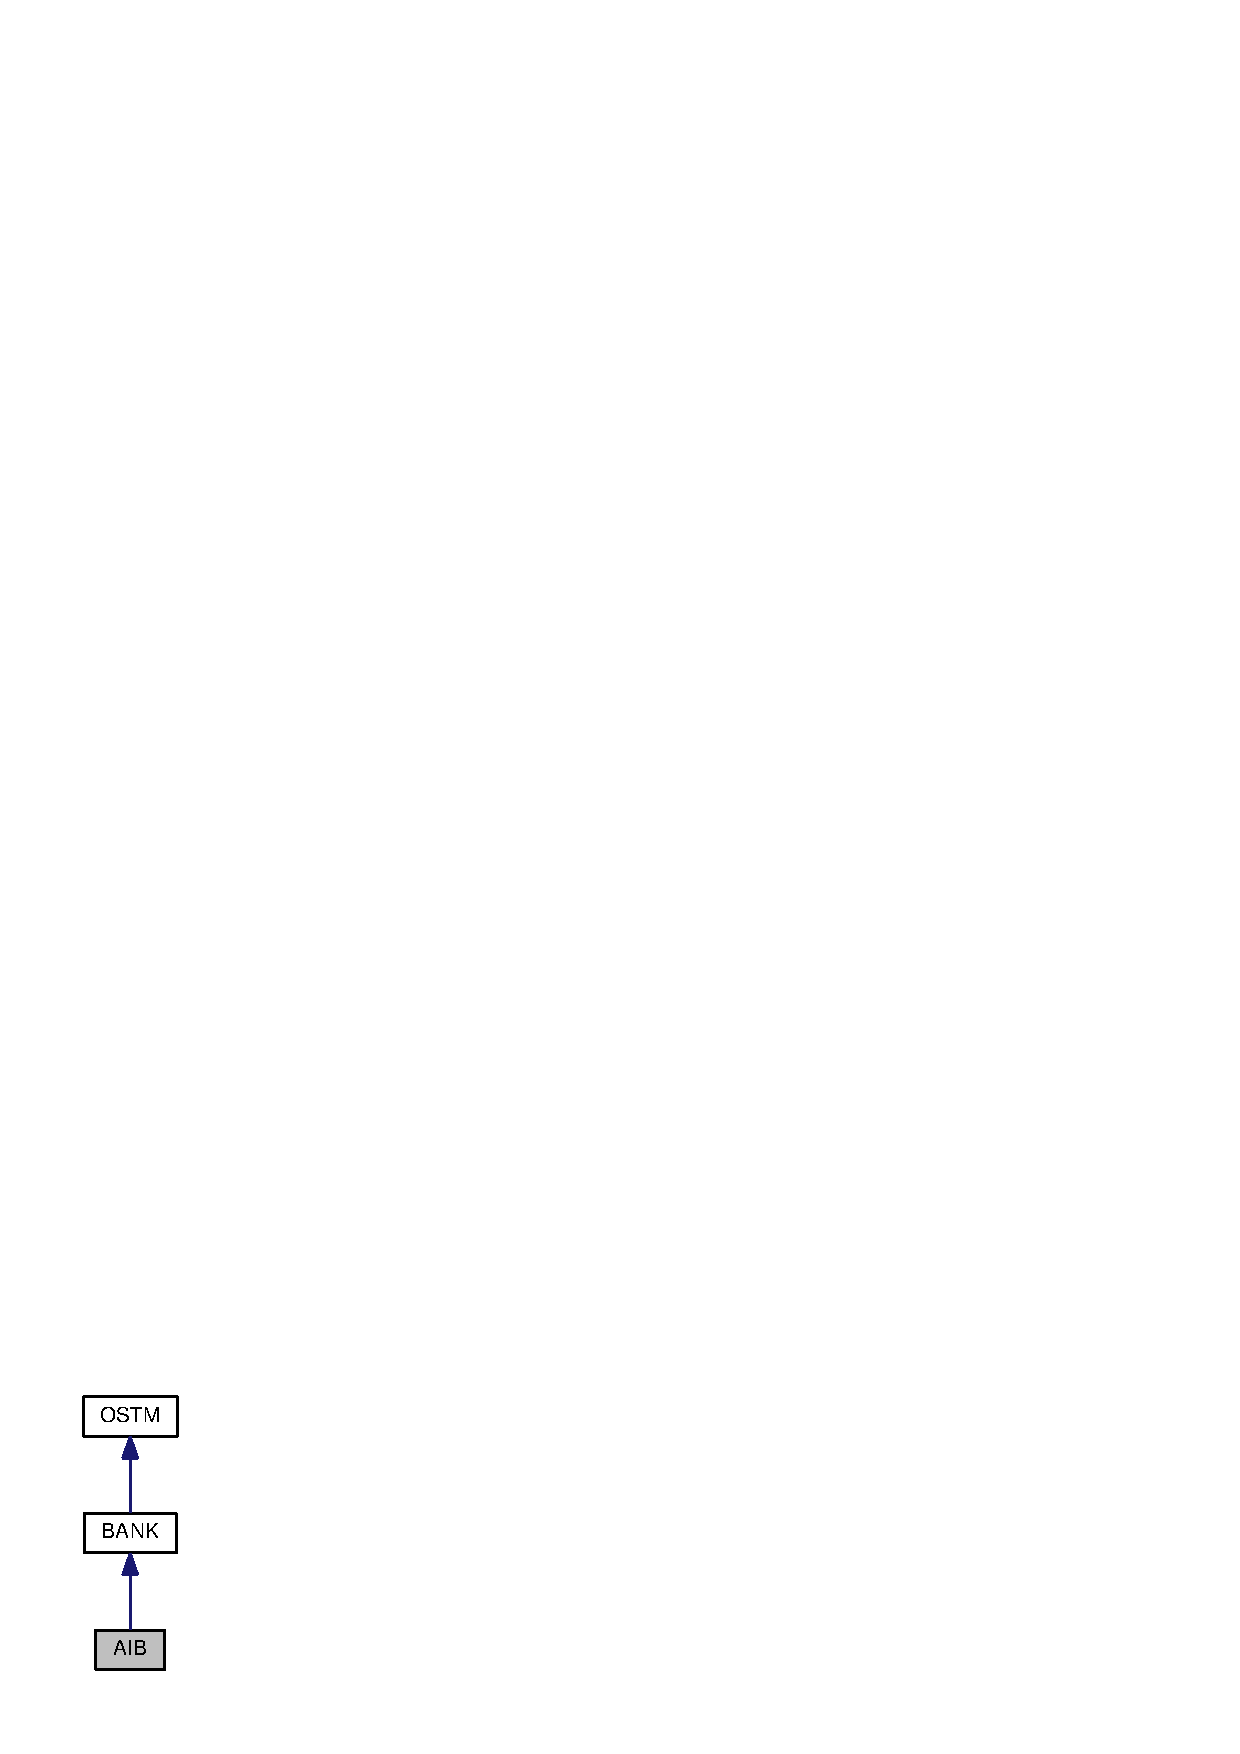
\includegraphics[height=550pt]{class_a_i_b__inherit__graph}
\end{center}
\end{figure}


Collaboration diagram for A\+IB\+:
\nopagebreak
\begin{figure}[H]
\begin{center}
\leavevmode
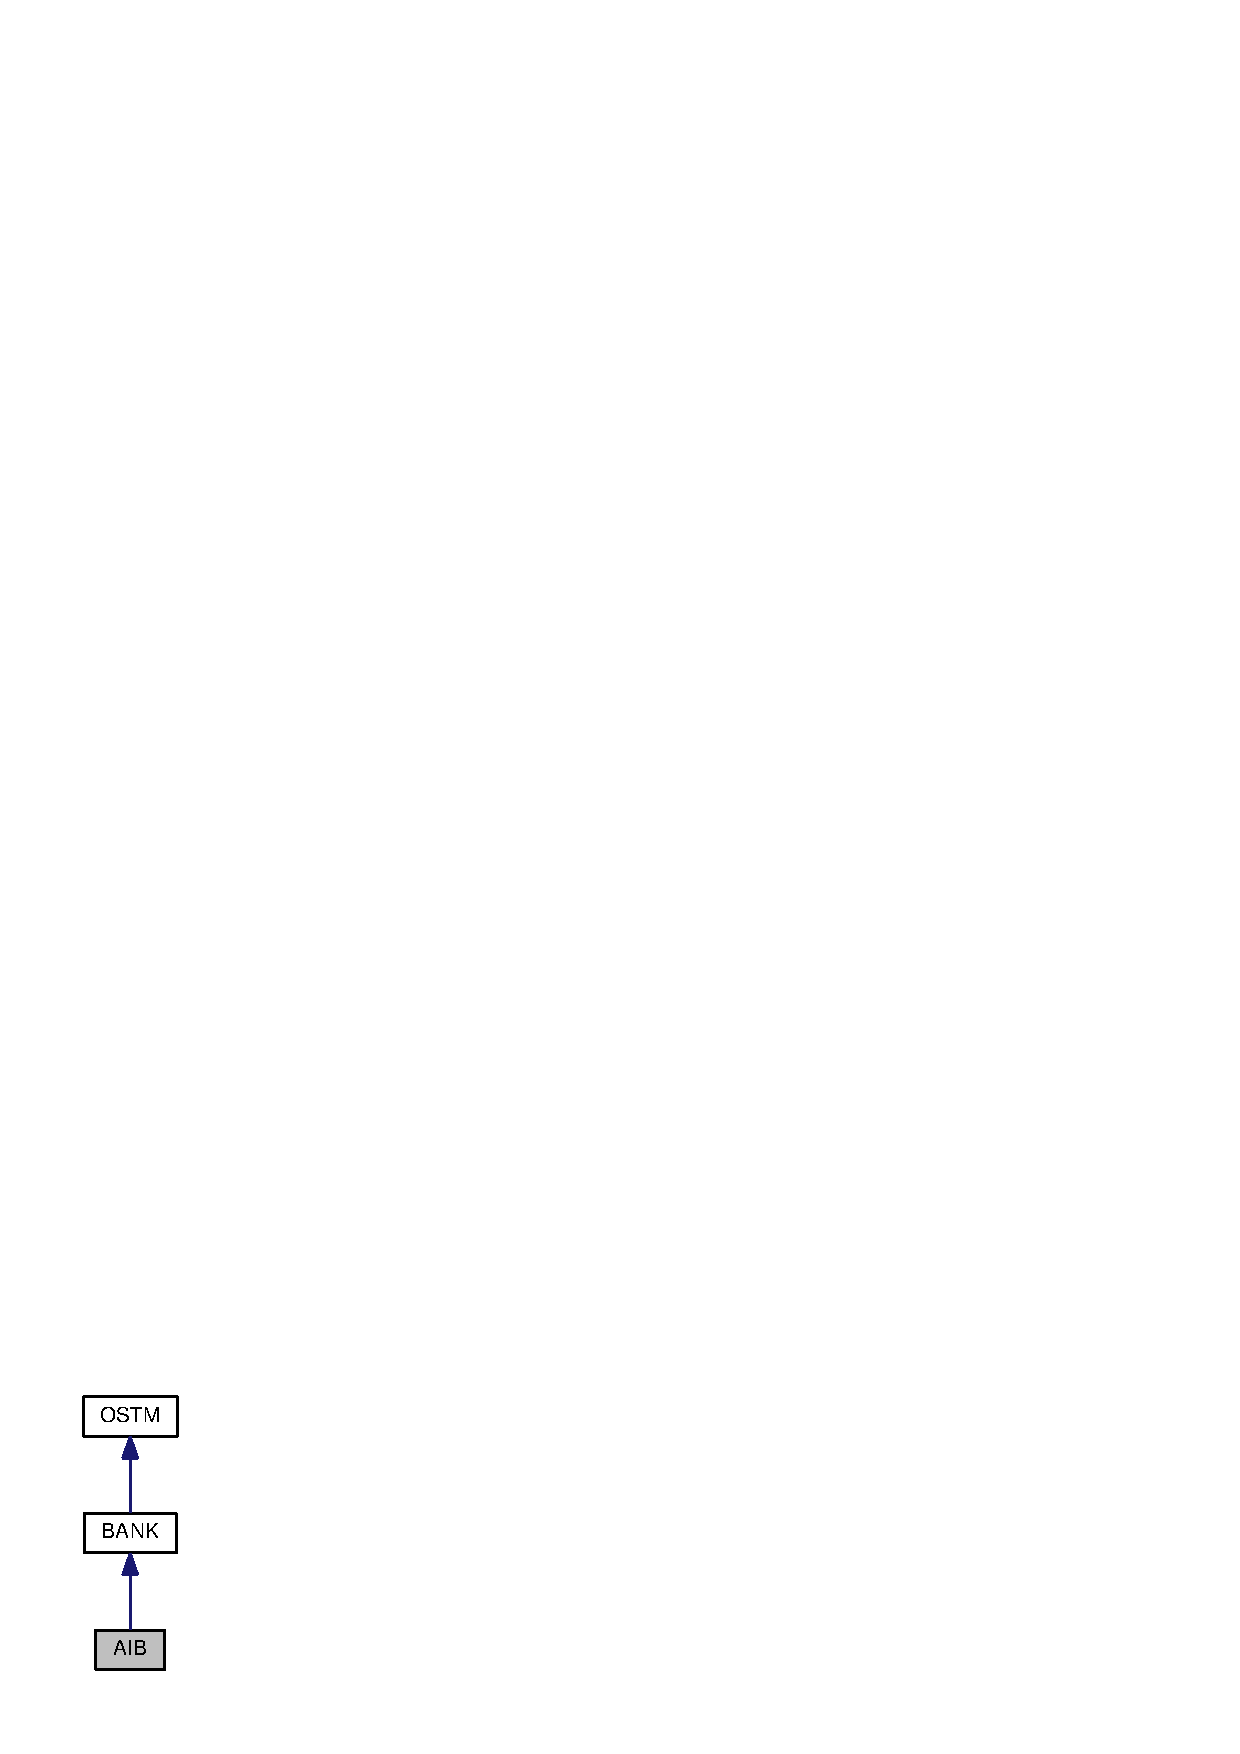
\includegraphics[height=550pt]{class_a_i_b__coll__graph}
\end{center}
\end{figure}
\subsubsection*{Public Member Functions}
\begin{DoxyCompactItemize}
\item 
\hyperlink{class_a_i_b_a4783110463bf12f937a85b62455faf38_a4783110463bf12f937a85b62455faf38}{A\+IB} ()
\item 
\hyperlink{class_a_i_b_a5fe3963becf294f6b1ce1a747f9122a0_a5fe3963becf294f6b1ce1a747f9122a0}{A\+IB} (int \hyperlink{class_a_i_b_aafc08efeec5b8c800c32ee32f20603a7_aafc08efeec5b8c800c32ee32f20603a7}{account\+Number}, double \hyperlink{class_a_i_b_a3c8d637bd997c1f062d844a88e2559ba_a3c8d637bd997c1f062d844a88e2559ba}{balance}, std\+::string \hyperlink{class_a_i_b_a869f72057cb63ebf0cfd257069e15c7c_a869f72057cb63ebf0cfd257069e15c7c}{first\+Name}, std\+::string \hyperlink{class_a_i_b_ace7b8b648d1b44b7ee2f4be002952b7a_ace7b8b648d1b44b7ee2f4be002952b7a}{last\+Name}, std\+::string \hyperlink{class_a_i_b_ae6a67cc33d1e5fa83a52a238e45ca3dc_ae6a67cc33d1e5fa83a52a238e45ca3dc}{address})
\item 
\hyperlink{class_a_i_b_aa0faccb7aadf423d12bddb2469ff5053_aa0faccb7aadf423d12bddb2469ff5053}{A\+IB} (std\+::shared\+\_\+ptr$<$ \hyperlink{class_b_a_n_k}{B\+A\+NK} $>$ obj, int \+\_\+version, int \+\_\+unique\+\_\+id)
\item 
\hyperlink{class_a_i_b_ab13d0db3498d59dbe6a946c469587c55_ab13d0db3498d59dbe6a946c469587c55}{A\+IB} (const \hyperlink{class_a_i_b}{A\+IB} \&orig)
\item 
virtual void \hyperlink{class_a_i_b_ad76f25ce86cb42028440f41c371903e0_ad76f25ce86cb42028440f41c371903e0}{copy} (std\+::shared\+\_\+ptr$<$ \hyperlink{class_o_s_t_m}{O\+S\+TM} $>$ to, std\+::shared\+\_\+ptr$<$ \hyperlink{class_o_s_t_m}{O\+S\+TM} $>$ from)
\begin{DoxyCompactList}\small\item\em copy function, make deep copy of the object/pointer \end{DoxyCompactList}\item 
virtual int \hyperlink{class_a_i_b_aef34bfbf20d767114e05b8b532cab777_aef34bfbf20d767114e05b8b532cab777}{Get\+Account\+Number} () const 
\begin{DoxyCompactList}\small\item\em Get\+Account\+Number getter for account\+Number private field. \end{DoxyCompactList}\item 
virtual std\+::string \hyperlink{class_a_i_b_a5092c8741fbe231531aa5aaa61d26b9c_a5092c8741fbe231531aa5aaa61d26b9c}{Get\+Address} () const 
\begin{DoxyCompactList}\small\item\em Get\+Address getter for address private field. \end{DoxyCompactList}\item 
virtual double \hyperlink{class_a_i_b_ac75087ae73c308bd946e47a71dc85b86_ac75087ae73c308bd946e47a71dc85b86}{Get\+Balance} () const 
\begin{DoxyCompactList}\small\item\em Get\+Balance getter for balance private field. \end{DoxyCompactList}\item 
virtual std\+::shared\+\_\+ptr$<$ \hyperlink{class_o_s_t_m}{O\+S\+TM} $>$ \hyperlink{class_a_i_b_a987107f3d7a04790f84c1e7eeee37575_a987107f3d7a04790f84c1e7eeee37575}{get\+Base\+Copy} (std\+::shared\+\_\+ptr$<$ \hyperlink{class_o_s_t_m}{O\+S\+TM} $>$ object)
\begin{DoxyCompactList}\small\item\em get\+Base\+Copy function, make deep copy of the object/pointer and Return a new std\+::shared\+\_\+ptr$<$\+B\+A\+N\+K$>$ type object \end{DoxyCompactList}\item 
virtual std\+::string \hyperlink{class_a_i_b_aa0833919c1c211481560cd88cb5b381b_aa0833919c1c211481560cd88cb5b381b}{Get\+First\+Name} () const 
\begin{DoxyCompactList}\small\item\em Get\+First\+Name getter for first\+Name private field. \end{DoxyCompactList}\item 
virtual std\+::string \hyperlink{class_a_i_b_a4fbad1d62d84d47e78b2b7065be14942_a4fbad1d62d84d47e78b2b7065be14942}{Get\+Fullname} () const 
\begin{DoxyCompactList}\small\item\em Get\+Fullname getter for fullname private field. \end{DoxyCompactList}\item 
virtual std\+::string \hyperlink{class_a_i_b_a1b09db7268734beeaf6a9e7e9d8feb02_a1b09db7268734beeaf6a9e7e9d8feb02}{Get\+Last\+Name} () const 
\begin{DoxyCompactList}\small\item\em Get\+Last\+Name getter for last\+Name private field. \end{DoxyCompactList}\item 
\hyperlink{class_a_i_b}{A\+IB} \hyperlink{class_a_i_b_a77b6f74ea3ef39cb1ccb916db7a48740_a77b6f74ea3ef39cb1ccb916db7a48740}{operator=} (const \hyperlink{class_a_i_b}{A\+IB} \&orig)
\item 
virtual void \hyperlink{class_a_i_b_ae582677d2d890f1728dedb9f43965df6_ae582677d2d890f1728dedb9f43965df6}{Set\+Account\+Number} (int \hyperlink{class_a_i_b_aafc08efeec5b8c800c32ee32f20603a7_aafc08efeec5b8c800c32ee32f20603a7}{account\+Number})
\begin{DoxyCompactList}\small\item\em Set\+Account\+Number setter for account\+Number private field. \end{DoxyCompactList}\item 
virtual void \hyperlink{class_a_i_b_ab5fd22fbbc0ea75a022aaeb7174fc450_ab5fd22fbbc0ea75a022aaeb7174fc450}{Set\+Address} (std\+::string \hyperlink{class_a_i_b_ae6a67cc33d1e5fa83a52a238e45ca3dc_ae6a67cc33d1e5fa83a52a238e45ca3dc}{address})
\begin{DoxyCompactList}\small\item\em Set\+Address setter for address private field. \end{DoxyCompactList}\item 
virtual void \hyperlink{class_a_i_b_ac286e13b8cf985bc88ce356b0eaada81_ac286e13b8cf985bc88ce356b0eaada81}{Set\+Balance} (double \hyperlink{class_a_i_b_a3c8d637bd997c1f062d844a88e2559ba_a3c8d637bd997c1f062d844a88e2559ba}{balance})
\begin{DoxyCompactList}\small\item\em Set\+Balance setter for balance private field. \end{DoxyCompactList}\item 
virtual void \hyperlink{class_a_i_b_a671e44bdbf1286d97d7a22295177dd2e_a671e44bdbf1286d97d7a22295177dd2e}{Set\+First\+Name} (std\+::string \hyperlink{class_a_i_b_a869f72057cb63ebf0cfd257069e15c7c_a869f72057cb63ebf0cfd257069e15c7c}{first\+Name})
\begin{DoxyCompactList}\small\item\em Set\+First\+Name setter for first\+Name private field. \end{DoxyCompactList}\item 
virtual void \hyperlink{class_a_i_b_a03def15426e627042951369ea18b97f6_a03def15426e627042951369ea18b97f6}{Set\+Fullname} (std\+::string \hyperlink{class_a_i_b_a818b0cc283af23127c067fb3fc751058_a818b0cc283af23127c067fb3fc751058}{fullname})
\begin{DoxyCompactList}\small\item\em Set\+Fullname setter for fullname private field. \end{DoxyCompactList}\item 
virtual void \hyperlink{class_a_i_b_afe4e3c7b481bf87437968dde2cc75882_afe4e3c7b481bf87437968dde2cc75882}{Set\+Last\+Name} (std\+::string \hyperlink{class_a_i_b_ace7b8b648d1b44b7ee2f4be002952b7a_ace7b8b648d1b44b7ee2f4be002952b7a}{last\+Name})
\begin{DoxyCompactList}\small\item\em Set\+Last\+Name setter for last\+Name private field. \end{DoxyCompactList}\item 
virtual void \hyperlink{class_a_i_b_aff0f0a0db75a17efec4bd500b888232d_aff0f0a0db75a17efec4bd500b888232d}{to\+String} ()
\begin{DoxyCompactList}\small\item\em to\+String function, displays the object values in formatted way \end{DoxyCompactList}\item 
virtual \hyperlink{class_a_i_b_a22b11c50b0986326c86315957528bf79_a22b11c50b0986326c86315957528bf79}{$\sim$\+A\+IB} ()
\end{DoxyCompactItemize}
\subsubsection*{Private Attributes}
\begin{DoxyCompactItemize}
\item 
int \hyperlink{class_a_i_b_aafc08efeec5b8c800c32ee32f20603a7_aafc08efeec5b8c800c32ee32f20603a7}{account\+Number}
\item 
std\+::string \hyperlink{class_a_i_b_ae6a67cc33d1e5fa83a52a238e45ca3dc_ae6a67cc33d1e5fa83a52a238e45ca3dc}{address}
\item 
double \hyperlink{class_a_i_b_a3c8d637bd997c1f062d844a88e2559ba_a3c8d637bd997c1f062d844a88e2559ba}{balance}
\item 
std\+::string \hyperlink{class_a_i_b_a869f72057cb63ebf0cfd257069e15c7c_a869f72057cb63ebf0cfd257069e15c7c}{first\+Name}
\item 
std\+::string \hyperlink{class_a_i_b_a818b0cc283af23127c067fb3fc751058_a818b0cc283af23127c067fb3fc751058}{fullname}
\item 
std\+::string \hyperlink{class_a_i_b_ace7b8b648d1b44b7ee2f4be002952b7a_ace7b8b648d1b44b7ee2f4be002952b7a}{last\+Name}
\end{DoxyCompactItemize}


\subsubsection{Detailed Description}
Class \hyperlink{class_a_i_b}{A\+IB} Inherit from \hyperlink{class_b_a_n_k}{B\+A\+NK} class 

Definition at line \hyperlink{_a_i_b_8h_source_l00023}{23} of file \hyperlink{_a_i_b_8h_source}{A\+I\+B.\+h}.



\subsubsection{Constructor \& Destructor Documentation}
\index{A\+IB@{A\+IB}!A\+IB@{A\+IB}}
\index{A\+IB@{A\+IB}!A\+IB@{A\+IB}}
\paragraph[{\texorpdfstring{A\+I\+B()}{AIB()}}]{\setlength{\rightskip}{0pt plus 5cm}A\+I\+B\+::\+A\+IB (
\begin{DoxyParamCaption}
{}
\end{DoxyParamCaption}
)\hspace{0.3cm}{\ttfamily [inline]}}\hypertarget{class_a_i_b_a4783110463bf12f937a85b62455faf38_a4783110463bf12f937a85b62455faf38}{}\label{class_a_i_b_a4783110463bf12f937a85b62455faf38_a4783110463bf12f937a85b62455faf38}
Constructor 

Definition at line \hyperlink{_a_i_b_8h_source_l00028}{28} of file \hyperlink{_a_i_b_8h_source}{A\+I\+B.\+h}.



References \hyperlink{_a_i_b_8h_source_l00123}{account\+Number}, \hyperlink{_a_i_b_8h_source_l00131}{address}, \hyperlink{_a_i_b_8h_source_l00127}{balance}, \hyperlink{_a_i_b_8h_source_l00115}{first\+Name}, \hyperlink{_a_i_b_8h_source_l00111}{fullname}, and \hyperlink{_a_i_b_8h_source_l00119}{last\+Name}.



Referenced by \hyperlink{_a_i_b_8h_source_l00061}{A\+I\+B()}, and \hyperlink{_a_i_b_8cpp_source_l00025}{get\+Base\+Copy()}.


\begin{DoxyCode}
00028          : \hyperlink{class_b_a_n_k_a0bc938356cebff14fb0560264abe5a34_a0bc938356cebff14fb0560264abe5a34}{BANK}()
00029     \{
00030         this->\hyperlink{class_a_i_b_aafc08efeec5b8c800c32ee32f20603a7_aafc08efeec5b8c800c32ee32f20603a7}{accountNumber} = 0;
00031         this->\hyperlink{class_a_i_b_a3c8d637bd997c1f062d844a88e2559ba_a3c8d637bd997c1f062d844a88e2559ba}{balance} = 50;
00032         this->\hyperlink{class_a_i_b_a869f72057cb63ebf0cfd257069e15c7c_a869f72057cb63ebf0cfd257069e15c7c}{firstName} = \textcolor{stringliteral}{"Joe"};
00033         this->\hyperlink{class_a_i_b_ace7b8b648d1b44b7ee2f4be002952b7a_ace7b8b648d1b44b7ee2f4be002952b7a}{lastName} = \textcolor{stringliteral}{"Blog"};
00034         this->\hyperlink{class_a_i_b_ae6a67cc33d1e5fa83a52a238e45ca3dc_ae6a67cc33d1e5fa83a52a238e45ca3dc}{address} = \textcolor{stringliteral}{"High street, Carlow"};
00035         this->\hyperlink{class_a_i_b_a818b0cc283af23127c067fb3fc751058_a818b0cc283af23127c067fb3fc751058}{fullname} = \hyperlink{class_a_i_b_a869f72057cb63ebf0cfd257069e15c7c_a869f72057cb63ebf0cfd257069e15c7c}{firstName} + \textcolor{stringliteral}{" "} + \hyperlink{class_a_i_b_ace7b8b648d1b44b7ee2f4be002952b7a_ace7b8b648d1b44b7ee2f4be002952b7a}{lastName};
00036     
00037     \};
\end{DoxyCode}


Here is the caller graph for this function\+:\nopagebreak
\begin{figure}[H]
\begin{center}
\leavevmode
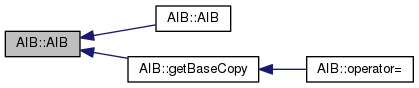
\includegraphics[width=350pt]{class_a_i_b_a4783110463bf12f937a85b62455faf38_a4783110463bf12f937a85b62455faf38_icgraph}
\end{center}
\end{figure}


\index{A\+IB@{A\+IB}!A\+IB@{A\+IB}}
\index{A\+IB@{A\+IB}!A\+IB@{A\+IB}}
\paragraph[{\texorpdfstring{A\+I\+B(int account\+Number, double balance, std\+::string first\+Name, std\+::string last\+Name, std\+::string address)}{AIB(int accountNumber, double balance, std::string firstName, std::string lastName, std::string address)}}]{\setlength{\rightskip}{0pt plus 5cm}A\+I\+B\+::\+A\+IB (
\begin{DoxyParamCaption}
\item[{int}]{account\+Number, }
\item[{double}]{balance, }
\item[{std\+::string}]{first\+Name, }
\item[{std\+::string}]{last\+Name, }
\item[{std\+::string}]{address}
\end{DoxyParamCaption}
)\hspace{0.3cm}{\ttfamily [inline]}}\hypertarget{class_a_i_b_a5fe3963becf294f6b1ce1a747f9122a0_a5fe3963becf294f6b1ce1a747f9122a0}{}\label{class_a_i_b_a5fe3963becf294f6b1ce1a747f9122a0_a5fe3963becf294f6b1ce1a747f9122a0}
Custom constructor 
\begin{DoxyParams}{Parameters}
{\em account\+Number} & integer \\
\hline
{\em balance} & double \\
\hline
{\em first\+Name} & string \\
\hline
{\em last\+Name} & string \\
\hline
{\em address} & string \\
\hline
\end{DoxyParams}


Definition at line \hyperlink{_a_i_b_8h_source_l00046}{46} of file \hyperlink{_a_i_b_8h_source}{A\+I\+B.\+h}.



References \hyperlink{_a_i_b_8h_source_l00123}{account\+Number}, \hyperlink{_a_i_b_8h_source_l00131}{address}, \hyperlink{_a_i_b_8h_source_l00127}{balance}, \hyperlink{_a_i_b_8h_source_l00115}{first\+Name}, \hyperlink{_a_i_b_8h_source_l00111}{fullname}, and \hyperlink{_a_i_b_8h_source_l00119}{last\+Name}.


\begin{DoxyCode}
00046                                                                                                       : 
      \hyperlink{class_b_a_n_k_a0bc938356cebff14fb0560264abe5a34_a0bc938356cebff14fb0560264abe5a34}{BANK}()
00047     \{
00048         this->\hyperlink{class_a_i_b_aafc08efeec5b8c800c32ee32f20603a7_aafc08efeec5b8c800c32ee32f20603a7}{accountNumber} = \hyperlink{class_a_i_b_aafc08efeec5b8c800c32ee32f20603a7_aafc08efeec5b8c800c32ee32f20603a7}{accountNumber};
00049         this->\hyperlink{class_a_i_b_a3c8d637bd997c1f062d844a88e2559ba_a3c8d637bd997c1f062d844a88e2559ba}{balance} = \hyperlink{class_a_i_b_a3c8d637bd997c1f062d844a88e2559ba_a3c8d637bd997c1f062d844a88e2559ba}{balance};
00050         this->\hyperlink{class_a_i_b_a869f72057cb63ebf0cfd257069e15c7c_a869f72057cb63ebf0cfd257069e15c7c}{firstName} = \hyperlink{class_a_i_b_a869f72057cb63ebf0cfd257069e15c7c_a869f72057cb63ebf0cfd257069e15c7c}{firstName};
00051         this->\hyperlink{class_a_i_b_ace7b8b648d1b44b7ee2f4be002952b7a_ace7b8b648d1b44b7ee2f4be002952b7a}{lastName} = \hyperlink{class_a_i_b_ace7b8b648d1b44b7ee2f4be002952b7a_ace7b8b648d1b44b7ee2f4be002952b7a}{lastName};
00052         this->\hyperlink{class_a_i_b_ae6a67cc33d1e5fa83a52a238e45ca3dc_ae6a67cc33d1e5fa83a52a238e45ca3dc}{address} = \hyperlink{class_a_i_b_ae6a67cc33d1e5fa83a52a238e45ca3dc_ae6a67cc33d1e5fa83a52a238e45ca3dc}{address};
00053         this->\hyperlink{class_a_i_b_a818b0cc283af23127c067fb3fc751058_a818b0cc283af23127c067fb3fc751058}{fullname} = \hyperlink{class_a_i_b_a869f72057cb63ebf0cfd257069e15c7c_a869f72057cb63ebf0cfd257069e15c7c}{firstName} + \textcolor{stringliteral}{" "} + \hyperlink{class_a_i_b_ace7b8b648d1b44b7ee2f4be002952b7a_ace7b8b648d1b44b7ee2f4be002952b7a}{lastName};
00054     \}; 
\end{DoxyCode}
\index{A\+IB@{A\+IB}!A\+IB@{A\+IB}}
\index{A\+IB@{A\+IB}!A\+IB@{A\+IB}}
\paragraph[{\texorpdfstring{A\+I\+B(std\+::shared\+\_\+ptr$<$ B\+A\+N\+K $>$ obj, int \+\_\+version, int \+\_\+unique\+\_\+id)}{AIB(std::shared_ptr< BANK > obj, int _version, int _unique_id)}}]{\setlength{\rightskip}{0pt plus 5cm}A\+I\+B\+::\+A\+IB (
\begin{DoxyParamCaption}
\item[{std\+::shared\+\_\+ptr$<$ {\bf B\+A\+NK} $>$}]{obj, }
\item[{int}]{\+\_\+version, }
\item[{int}]{\+\_\+unique\+\_\+id}
\end{DoxyParamCaption}
)\hspace{0.3cm}{\ttfamily [inline]}}\hypertarget{class_a_i_b_aa0faccb7aadf423d12bddb2469ff5053_aa0faccb7aadf423d12bddb2469ff5053}{}\label{class_a_i_b_aa0faccb7aadf423d12bddb2469ff5053_aa0faccb7aadf423d12bddb2469ff5053}
Custom constructor, used by the library for deep copying 
\begin{DoxyParams}{Parameters}
{\em obj} & std\+::shared\+\_\+ptr$<$\+B\+A\+N\+K$>$ \\
\hline
{\em \+\_\+version} & integer \\
\hline
{\em \+\_\+unique\+\_\+id} & integer \\
\hline
\end{DoxyParams}


Definition at line \hyperlink{_a_i_b_8h_source_l00061}{61} of file \hyperlink{_a_i_b_8h_source}{A\+I\+B.\+h}.



References \hyperlink{_a_i_b_8h_source_l00123}{account\+Number}, \hyperlink{_a_i_b_8h_source_l00131}{address}, \hyperlink{_a_i_b_8h_source_l00028}{A\+I\+B()}, \hyperlink{_a_i_b_8h_source_l00127}{balance}, \hyperlink{_a_i_b_8h_source_l00115}{first\+Name}, \hyperlink{_a_i_b_8h_source_l00111}{fullname}, and \hyperlink{_a_i_b_8h_source_l00119}{last\+Name}.


\begin{DoxyCode}
00061                                                               : \hyperlink{class_b_a_n_k_a0bc938356cebff14fb0560264abe5a34_a0bc938356cebff14fb0560264abe5a34}{BANK}(\_version, \_unique\_id)
00062     \{
00063         this->\hyperlink{class_a_i_b_aafc08efeec5b8c800c32ee32f20603a7_aafc08efeec5b8c800c32ee32f20603a7}{accountNumber} = obj->GetAccountNumber();
00064         this->\hyperlink{class_a_i_b_a3c8d637bd997c1f062d844a88e2559ba_a3c8d637bd997c1f062d844a88e2559ba}{balance} = obj->GetBalance();
00065         this->\hyperlink{class_a_i_b_a869f72057cb63ebf0cfd257069e15c7c_a869f72057cb63ebf0cfd257069e15c7c}{firstName} = obj->GetFirstName();
00066         this->\hyperlink{class_a_i_b_ace7b8b648d1b44b7ee2f4be002952b7a_ace7b8b648d1b44b7ee2f4be002952b7a}{lastName} = obj->GetLastName();
00067         this->\hyperlink{class_a_i_b_ae6a67cc33d1e5fa83a52a238e45ca3dc_ae6a67cc33d1e5fa83a52a238e45ca3dc}{address} = obj->GetAddress();
00068         this->\hyperlink{class_a_i_b_a818b0cc283af23127c067fb3fc751058_a818b0cc283af23127c067fb3fc751058}{fullname} = obj->GetFirstName() + \textcolor{stringliteral}{" "} + obj->GetLastName(); 
00069         
00070     \};
\end{DoxyCode}


Here is the call graph for this function\+:\nopagebreak
\begin{figure}[H]
\begin{center}
\leavevmode
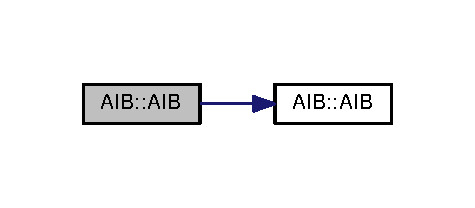
\includegraphics[width=228pt]{class_a_i_b_aa0faccb7aadf423d12bddb2469ff5053_aa0faccb7aadf423d12bddb2469ff5053_cgraph}
\end{center}
\end{figure}


\index{A\+IB@{A\+IB}!A\+IB@{A\+IB}}
\index{A\+IB@{A\+IB}!A\+IB@{A\+IB}}
\paragraph[{\texorpdfstring{A\+I\+B(const A\+I\+B \&orig)}{AIB(const AIB &orig)}}]{\setlength{\rightskip}{0pt plus 5cm}A\+I\+B\+::\+A\+IB (
\begin{DoxyParamCaption}
\item[{const {\bf A\+IB} \&}]{orig}
\end{DoxyParamCaption}
)}\hypertarget{class_a_i_b_ab13d0db3498d59dbe6a946c469587c55_ab13d0db3498d59dbe6a946c469587c55}{}\label{class_a_i_b_ab13d0db3498d59dbe6a946c469587c55_ab13d0db3498d59dbe6a946c469587c55}
Copy constructor \index{A\+IB@{A\+IB}!````~A\+IB@{$\sim$\+A\+IB}}
\index{````~A\+IB@{$\sim$\+A\+IB}!A\+IB@{A\+IB}}
\paragraph[{\texorpdfstring{$\sim$\+A\+I\+B()}{~AIB()}}]{\setlength{\rightskip}{0pt plus 5cm}A\+I\+B\+::$\sim$\+A\+IB (
\begin{DoxyParamCaption}
{}
\end{DoxyParamCaption}
)\hspace{0.3cm}{\ttfamily [virtual]}}\hypertarget{class_a_i_b_a22b11c50b0986326c86315957528bf79_a22b11c50b0986326c86315957528bf79}{}\label{class_a_i_b_a22b11c50b0986326c86315957528bf79_a22b11c50b0986326c86315957528bf79}
de-\/constructor 

Definition at line \hyperlink{_a_i_b_8cpp_source_l00019}{19} of file \hyperlink{_a_i_b_8cpp_source}{A\+I\+B.\+cpp}.



Referenced by \hyperlink{_a_i_b_8h_source_l00078}{operator=()}.


\begin{DoxyCode}
00019           \{
00020 \}
\end{DoxyCode}


Here is the caller graph for this function\+:\nopagebreak
\begin{figure}[H]
\begin{center}
\leavevmode
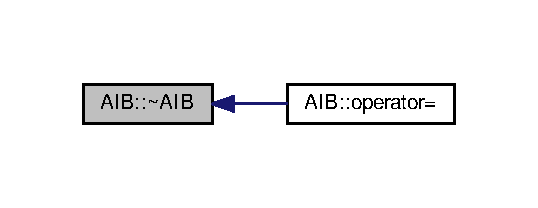
\includegraphics[width=258pt]{class_a_i_b_a22b11c50b0986326c86315957528bf79_a22b11c50b0986326c86315957528bf79_icgraph}
\end{center}
\end{figure}




\subsubsection{Member Function Documentation}
\index{A\+IB@{A\+IB}!copy@{copy}}
\index{copy@{copy}!A\+IB@{A\+IB}}
\paragraph[{\texorpdfstring{copy(std\+::shared\+\_\+ptr$<$ O\+S\+T\+M $>$ to, std\+::shared\+\_\+ptr$<$ O\+S\+T\+M $>$ from)}{copy(std::shared_ptr< OSTM > to, std::shared_ptr< OSTM > from)}}]{\setlength{\rightskip}{0pt plus 5cm}void A\+I\+B\+::copy (
\begin{DoxyParamCaption}
\item[{std\+::shared\+\_\+ptr$<$ {\bf O\+S\+TM} $>$}]{to, }
\item[{std\+::shared\+\_\+ptr$<$ {\bf O\+S\+TM} $>$}]{from}
\end{DoxyParamCaption}
)\hspace{0.3cm}{\ttfamily [virtual]}}\hypertarget{class_a_i_b_ad76f25ce86cb42028440f41c371903e0_ad76f25ce86cb42028440f41c371903e0}{}\label{class_a_i_b_ad76f25ce86cb42028440f41c371903e0_ad76f25ce86cb42028440f41c371903e0}


copy function, make deep copy of the object/pointer 

Implement \hyperlink{class_o_s_t_m}{O\+S\+TM} virtual methods in cpp class


\begin{DoxyParams}{Parameters}
{\em to} & std\+::shared\+\_\+ptr$<$\+O\+S\+T\+M$>$, \hyperlink{class_b_a_n_k}{B\+A\+NK} type shared pointer used to copy into the values \\
\hline
{\em from} & std\+::shared\+\_\+ptr$<$\+O\+S\+T\+M$>$, \hyperlink{class_b_a_n_k}{B\+A\+NK} type shared ponter used to get object values tfrom copy \\
\hline
\end{DoxyParams}
Dynamic cast from \hyperlink{class_o_s_t_m}{O\+S\+TM} to \hyperlink{class_a_i_b}{A\+IB}

Dynamic cast from \hyperlink{class_o_s_t_m}{O\+S\+TM} to \hyperlink{class_a_i_b}{A\+IB}

Set values fro object to object

Set values fro object to object

Set values fro object to object

Set values fro object to object 

Reimplemented from \hyperlink{class_o_s_t_m_a535d90fced5adbb70312c92f3778e08d_a535d90fced5adbb70312c92f3778e08d}{O\+S\+TM}.



Definition at line \hyperlink{_a_i_b_8cpp_source_l00041}{41} of file \hyperlink{_a_i_b_8cpp_source}{A\+I\+B.\+cpp}.



References \hyperlink{_o_s_t_m_8cpp_source_l00075}{O\+S\+T\+M\+::\+Set\+\_\+\+Unique\+\_\+\+I\+D()}.



Referenced by \hyperlink{_a_i_b_8h_source_l00078}{operator=()}.


\begin{DoxyCode}
00041                                                               \{
00042 
00044     std::shared\_ptr<AIB> objTO = std::dynamic\_pointer\_cast<\hyperlink{class_a_i_b}{AIB}>(to);
00046     std::shared\_ptr<AIB> objFROM = std::dynamic\_pointer\_cast<\hyperlink{class_a_i_b}{AIB}>(from);
00048     objTO->\hyperlink{class_o_s_t_m_ab5019a32185631c08abbf826422f2d93_ab5019a32185631c08abbf826422f2d93}{Set\_Unique\_ID}(objFROM->Get\_Unique\_ID());
00050     objTO->Set\_Version(objFROM->Get\_Version());
00052     objTO->SetAccountNumber(objFROM->GetAccountNumber());
00054     objTO->SetBalance(objFROM->GetBalance());
00055 \}
\end{DoxyCode}


Here is the call graph for this function\+:\nopagebreak
\begin{figure}[H]
\begin{center}
\leavevmode
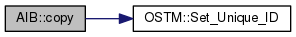
\includegraphics[width=294pt]{class_a_i_b_ad76f25ce86cb42028440f41c371903e0_ad76f25ce86cb42028440f41c371903e0_cgraph}
\end{center}
\end{figure}




Here is the caller graph for this function\+:\nopagebreak
\begin{figure}[H]
\begin{center}
\leavevmode
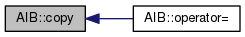
\includegraphics[width=256pt]{class_a_i_b_ad76f25ce86cb42028440f41c371903e0_ad76f25ce86cb42028440f41c371903e0_icgraph}
\end{center}
\end{figure}


\index{A\+IB@{A\+IB}!Get\+Account\+Number@{Get\+Account\+Number}}
\index{Get\+Account\+Number@{Get\+Account\+Number}!A\+IB@{A\+IB}}
\paragraph[{\texorpdfstring{Get\+Account\+Number() const }{GetAccountNumber() const }}]{\setlength{\rightskip}{0pt plus 5cm}int A\+I\+B\+::\+Get\+Account\+Number (
\begin{DoxyParamCaption}
{}
\end{DoxyParamCaption}
) const\hspace{0.3cm}{\ttfamily [virtual]}}\hypertarget{class_a_i_b_aef34bfbf20d767114e05b8b532cab777_aef34bfbf20d767114e05b8b532cab777}{}\label{class_a_i_b_aef34bfbf20d767114e05b8b532cab777_aef34bfbf20d767114e05b8b532cab777}


Get\+Account\+Number getter for account\+Number private field. 



Reimplemented from \hyperlink{class_b_a_n_k_a62adf3cea60d863a4a10eeee485fa1aa_a62adf3cea60d863a4a10eeee485fa1aa}{B\+A\+NK}.



Definition at line \hyperlink{_a_i_b_8cpp_source_l00096}{96} of file \hyperlink{_a_i_b_8cpp_source}{A\+I\+B.\+cpp}.



References \hyperlink{_a_i_b_8h_source_l00123}{account\+Number}.



Referenced by \hyperlink{_a_i_b_8h_source_l00078}{operator=()}, and \hyperlink{_a_i_b_8cpp_source_l00059}{to\+String()}.


\begin{DoxyCode}
00096                                 \{
00097     \textcolor{keywordflow}{return} \hyperlink{class_a_i_b_aafc08efeec5b8c800c32ee32f20603a7_aafc08efeec5b8c800c32ee32f20603a7}{accountNumber};
00098 \}
\end{DoxyCode}


Here is the caller graph for this function\+:\nopagebreak
\begin{figure}[H]
\begin{center}
\leavevmode
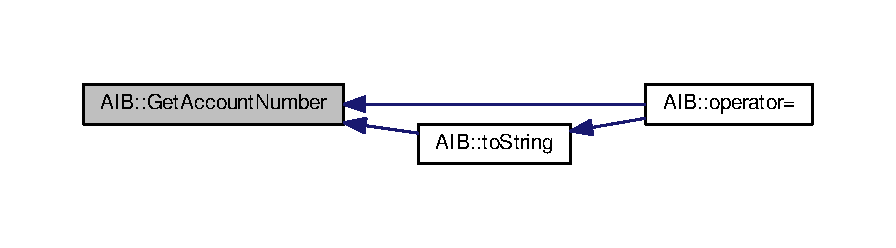
\includegraphics[width=350pt]{class_a_i_b_aef34bfbf20d767114e05b8b532cab777_aef34bfbf20d767114e05b8b532cab777_icgraph}
\end{center}
\end{figure}


\index{A\+IB@{A\+IB}!Get\+Address@{Get\+Address}}
\index{Get\+Address@{Get\+Address}!A\+IB@{A\+IB}}
\paragraph[{\texorpdfstring{Get\+Address() const }{GetAddress() const }}]{\setlength{\rightskip}{0pt plus 5cm}std\+::string A\+I\+B\+::\+Get\+Address (
\begin{DoxyParamCaption}
{}
\end{DoxyParamCaption}
) const\hspace{0.3cm}{\ttfamily [virtual]}}\hypertarget{class_a_i_b_a5092c8741fbe231531aa5aaa61d26b9c_a5092c8741fbe231531aa5aaa61d26b9c}{}\label{class_a_i_b_a5092c8741fbe231531aa5aaa61d26b9c_a5092c8741fbe231531aa5aaa61d26b9c}


Get\+Address getter for address private field. 



Reimplemented from \hyperlink{class_b_a_n_k_a358741f647f9494026e02fd3fd27cde6_a358741f647f9494026e02fd3fd27cde6}{B\+A\+NK}.



Definition at line \hyperlink{_a_i_b_8cpp_source_l00072}{72} of file \hyperlink{_a_i_b_8cpp_source}{A\+I\+B.\+cpp}.



References \hyperlink{_a_i_b_8h_source_l00131}{address}.



Referenced by \hyperlink{_a_i_b_8h_source_l00078}{operator=()}.


\begin{DoxyCode}
00072                                 \{
00073     \textcolor{keywordflow}{return} \hyperlink{class_a_i_b_ae6a67cc33d1e5fa83a52a238e45ca3dc_ae6a67cc33d1e5fa83a52a238e45ca3dc}{address};
00074 \}
\end{DoxyCode}


Here is the caller graph for this function\+:\nopagebreak
\begin{figure}[H]
\begin{center}
\leavevmode
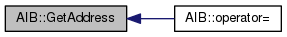
\includegraphics[width=287pt]{class_a_i_b_a5092c8741fbe231531aa5aaa61d26b9c_a5092c8741fbe231531aa5aaa61d26b9c_icgraph}
\end{center}
\end{figure}


\index{A\+IB@{A\+IB}!Get\+Balance@{Get\+Balance}}
\index{Get\+Balance@{Get\+Balance}!A\+IB@{A\+IB}}
\paragraph[{\texorpdfstring{Get\+Balance() const }{GetBalance() const }}]{\setlength{\rightskip}{0pt plus 5cm}double A\+I\+B\+::\+Get\+Balance (
\begin{DoxyParamCaption}
{}
\end{DoxyParamCaption}
) const\hspace{0.3cm}{\ttfamily [virtual]}}\hypertarget{class_a_i_b_ac75087ae73c308bd946e47a71dc85b86_ac75087ae73c308bd946e47a71dc85b86}{}\label{class_a_i_b_ac75087ae73c308bd946e47a71dc85b86_ac75087ae73c308bd946e47a71dc85b86}


Get\+Balance getter for balance private field. 



Reimplemented from \hyperlink{class_b_a_n_k_a7ac46c74859cebdc933cb27e148d18b1_a7ac46c74859cebdc933cb27e148d18b1}{B\+A\+NK}.



Definition at line \hyperlink{_a_i_b_8cpp_source_l00084}{84} of file \hyperlink{_a_i_b_8cpp_source}{A\+I\+B.\+cpp}.



References \hyperlink{_a_i_b_8h_source_l00127}{balance}.



Referenced by \hyperlink{_a_i_b_8h_source_l00078}{operator=()}, and \hyperlink{_a_i_b_8cpp_source_l00059}{to\+String()}.


\begin{DoxyCode}
00084                              \{
00085     \textcolor{keywordflow}{return} \hyperlink{class_a_i_b_a3c8d637bd997c1f062d844a88e2559ba_a3c8d637bd997c1f062d844a88e2559ba}{balance};
00086 \}
\end{DoxyCode}


Here is the caller graph for this function\+:\nopagebreak
\begin{figure}[H]
\begin{center}
\leavevmode
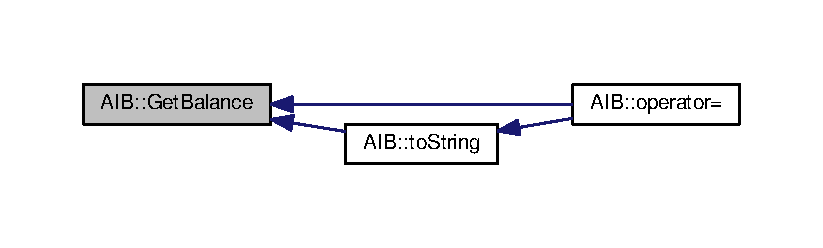
\includegraphics[width=350pt]{class_a_i_b_ac75087ae73c308bd946e47a71dc85b86_ac75087ae73c308bd946e47a71dc85b86_icgraph}
\end{center}
\end{figure}


\index{A\+IB@{A\+IB}!get\+Base\+Copy@{get\+Base\+Copy}}
\index{get\+Base\+Copy@{get\+Base\+Copy}!A\+IB@{A\+IB}}
\paragraph[{\texorpdfstring{get\+Base\+Copy(std\+::shared\+\_\+ptr$<$ O\+S\+T\+M $>$ object)}{getBaseCopy(std::shared_ptr< OSTM > object)}}]{\setlength{\rightskip}{0pt plus 5cm}std\+::shared\+\_\+ptr$<$ {\bf O\+S\+TM} $>$ A\+I\+B\+::get\+Base\+Copy (
\begin{DoxyParamCaption}
\item[{std\+::shared\+\_\+ptr$<$ {\bf O\+S\+TM} $>$}]{object}
\end{DoxyParamCaption}
)\hspace{0.3cm}{\ttfamily [virtual]}}\hypertarget{class_a_i_b_a987107f3d7a04790f84c1e7eeee37575_a987107f3d7a04790f84c1e7eeee37575}{}\label{class_a_i_b_a987107f3d7a04790f84c1e7eeee37575_a987107f3d7a04790f84c1e7eeee37575}


get\+Base\+Copy function, make deep copy of the object/pointer and Return a new std\+::shared\+\_\+ptr$<$\+B\+A\+N\+K$>$ type object 


\begin{DoxyParams}{Parameters}
{\em object} & is a \hyperlink{class_o_s_t_m}{O\+S\+TM} type shared pointer use to create a new copy of the pointer \\
\hline
\end{DoxyParams}
Dynamic cast from \hyperlink{class_o_s_t_m}{O\+S\+TM} to \hyperlink{class_b_a_n_k}{B\+A\+NK} type

\hyperlink{class_b_a_n_k}{B\+A\+NK} type Instance creation shared pointer

Dynamic cast from \hyperlink{class_b_a_n_k}{B\+A\+NK} to \hyperlink{class_o_s_t_m}{O\+S\+TM} type

Return new \hyperlink{class_o_s_t_m}{O\+S\+TM} copy onject 

Reimplemented from \hyperlink{class_o_s_t_m_a0bfa3763bd441407dd6365f42714f94c_a0bfa3763bd441407dd6365f42714f94c}{O\+S\+TM}.



Definition at line \hyperlink{_a_i_b_8cpp_source_l00025}{25} of file \hyperlink{_a_i_b_8cpp_source}{A\+I\+B.\+cpp}.



References \hyperlink{_a_i_b_8h_source_l00028}{A\+I\+B()}.



Referenced by \hyperlink{_a_i_b_8h_source_l00078}{operator=()}.


\begin{DoxyCode}
00026 \{
00028     std::shared\_ptr<BANK> objTO = std::dynamic\_pointer\_cast<\hyperlink{class_b_a_n_k}{BANK}>(object);
00030     std::shared\_ptr<BANK> obj(\textcolor{keyword}{new} \hyperlink{class_a_i_b_a4783110463bf12f937a85b62455faf38_a4783110463bf12f937a85b62455faf38}{AIB}(objTO, object->Get\_Version(),\textcolor{keywordtype}{object}->Get\_Unique\_ID()));
00032     std::shared\_ptr<OSTM> ostm\_obj = std::dynamic\_pointer\_cast<\hyperlink{class_o_s_t_m}{OSTM}>(obj);
00034     \textcolor{keywordflow}{return} ostm\_obj;
00035 \}
\end{DoxyCode}


Here is the call graph for this function\+:\nopagebreak
\begin{figure}[H]
\begin{center}
\leavevmode
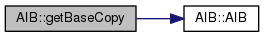
\includegraphics[width=270pt]{class_a_i_b_a987107f3d7a04790f84c1e7eeee37575_a987107f3d7a04790f84c1e7eeee37575_cgraph}
\end{center}
\end{figure}




Here is the caller graph for this function\+:\nopagebreak
\begin{figure}[H]
\begin{center}
\leavevmode
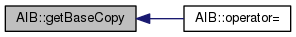
\includegraphics[width=294pt]{class_a_i_b_a987107f3d7a04790f84c1e7eeee37575_a987107f3d7a04790f84c1e7eeee37575_icgraph}
\end{center}
\end{figure}


\index{A\+IB@{A\+IB}!Get\+First\+Name@{Get\+First\+Name}}
\index{Get\+First\+Name@{Get\+First\+Name}!A\+IB@{A\+IB}}
\paragraph[{\texorpdfstring{Get\+First\+Name() const }{GetFirstName() const }}]{\setlength{\rightskip}{0pt plus 5cm}std\+::string A\+I\+B\+::\+Get\+First\+Name (
\begin{DoxyParamCaption}
{}
\end{DoxyParamCaption}
) const\hspace{0.3cm}{\ttfamily [virtual]}}\hypertarget{class_a_i_b_aa0833919c1c211481560cd88cb5b381b_aa0833919c1c211481560cd88cb5b381b}{}\label{class_a_i_b_aa0833919c1c211481560cd88cb5b381b_aa0833919c1c211481560cd88cb5b381b}


Get\+First\+Name getter for first\+Name private field. 



Reimplemented from \hyperlink{class_b_a_n_k_ad0ba1c785c67e7d4760dc8776f3d4bca_ad0ba1c785c67e7d4760dc8776f3d4bca}{B\+A\+NK}.



Definition at line \hyperlink{_a_i_b_8cpp_source_l00120}{120} of file \hyperlink{_a_i_b_8cpp_source}{A\+I\+B.\+cpp}.



References \hyperlink{_a_i_b_8h_source_l00115}{first\+Name}.



Referenced by \hyperlink{_a_i_b_8h_source_l00078}{operator=()}, and \hyperlink{_a_i_b_8cpp_source_l00059}{to\+String()}.


\begin{DoxyCode}
00120                                   \{
00121     \textcolor{keywordflow}{return} \hyperlink{class_a_i_b_a869f72057cb63ebf0cfd257069e15c7c_a869f72057cb63ebf0cfd257069e15c7c}{firstName};
00122 \}
\end{DoxyCode}


Here is the caller graph for this function\+:\nopagebreak
\begin{figure}[H]
\begin{center}
\leavevmode
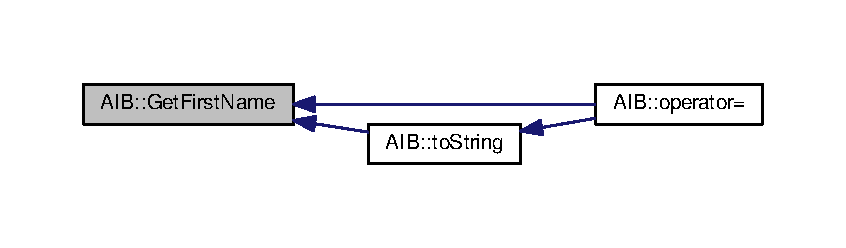
\includegraphics[width=350pt]{class_a_i_b_aa0833919c1c211481560cd88cb5b381b_aa0833919c1c211481560cd88cb5b381b_icgraph}
\end{center}
\end{figure}


\index{A\+IB@{A\+IB}!Get\+Fullname@{Get\+Fullname}}
\index{Get\+Fullname@{Get\+Fullname}!A\+IB@{A\+IB}}
\paragraph[{\texorpdfstring{Get\+Fullname() const }{GetFullname() const }}]{\setlength{\rightskip}{0pt plus 5cm}std\+::string A\+I\+B\+::\+Get\+Fullname (
\begin{DoxyParamCaption}
{}
\end{DoxyParamCaption}
) const\hspace{0.3cm}{\ttfamily [virtual]}}\hypertarget{class_a_i_b_a4fbad1d62d84d47e78b2b7065be14942_a4fbad1d62d84d47e78b2b7065be14942}{}\label{class_a_i_b_a4fbad1d62d84d47e78b2b7065be14942_a4fbad1d62d84d47e78b2b7065be14942}


Get\+Fullname getter for fullname private field. 



Reimplemented from \hyperlink{class_b_a_n_k_aa1528c533bf6389bc8d7f3eeca114bab_aa1528c533bf6389bc8d7f3eeca114bab}{B\+A\+NK}.



Definition at line \hyperlink{_a_i_b_8cpp_source_l00132}{132} of file \hyperlink{_a_i_b_8cpp_source}{A\+I\+B.\+cpp}.



References \hyperlink{_a_i_b_8h_source_l00111}{fullname}.



Referenced by \hyperlink{_a_i_b_8h_source_l00078}{operator=()}.


\begin{DoxyCode}
00132                                  \{
00133     \textcolor{keywordflow}{return} \hyperlink{class_a_i_b_a818b0cc283af23127c067fb3fc751058_a818b0cc283af23127c067fb3fc751058}{fullname};
00134 \}
\end{DoxyCode}


Here is the caller graph for this function\+:\nopagebreak
\begin{figure}[H]
\begin{center}
\leavevmode
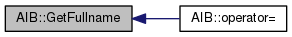
\includegraphics[width=291pt]{class_a_i_b_a4fbad1d62d84d47e78b2b7065be14942_a4fbad1d62d84d47e78b2b7065be14942_icgraph}
\end{center}
\end{figure}


\index{A\+IB@{A\+IB}!Get\+Last\+Name@{Get\+Last\+Name}}
\index{Get\+Last\+Name@{Get\+Last\+Name}!A\+IB@{A\+IB}}
\paragraph[{\texorpdfstring{Get\+Last\+Name() const }{GetLastName() const }}]{\setlength{\rightskip}{0pt plus 5cm}std\+::string A\+I\+B\+::\+Get\+Last\+Name (
\begin{DoxyParamCaption}
{}
\end{DoxyParamCaption}
) const\hspace{0.3cm}{\ttfamily [virtual]}}\hypertarget{class_a_i_b_a1b09db7268734beeaf6a9e7e9d8feb02_a1b09db7268734beeaf6a9e7e9d8feb02}{}\label{class_a_i_b_a1b09db7268734beeaf6a9e7e9d8feb02_a1b09db7268734beeaf6a9e7e9d8feb02}


Get\+Last\+Name getter for last\+Name private field. 



Reimplemented from \hyperlink{class_b_a_n_k_a4612063ec2bfd6d883a77a0d3697af90_a4612063ec2bfd6d883a77a0d3697af90}{B\+A\+NK}.



Definition at line \hyperlink{_a_i_b_8cpp_source_l00108}{108} of file \hyperlink{_a_i_b_8cpp_source}{A\+I\+B.\+cpp}.



References \hyperlink{_a_i_b_8h_source_l00119}{last\+Name}.



Referenced by \hyperlink{_a_i_b_8h_source_l00078}{operator=()}, and \hyperlink{_a_i_b_8cpp_source_l00059}{to\+String()}.


\begin{DoxyCode}
00108                                  \{
00109     \textcolor{keywordflow}{return} \hyperlink{class_a_i_b_ace7b8b648d1b44b7ee2f4be002952b7a_ace7b8b648d1b44b7ee2f4be002952b7a}{lastName};
00110 \}
\end{DoxyCode}


Here is the caller graph for this function\+:\nopagebreak
\begin{figure}[H]
\begin{center}
\leavevmode
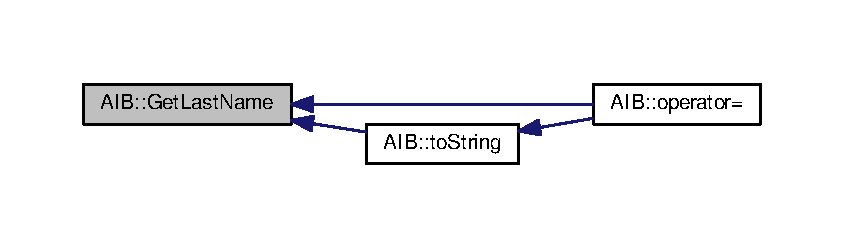
\includegraphics[width=350pt]{class_a_i_b_a1b09db7268734beeaf6a9e7e9d8feb02_a1b09db7268734beeaf6a9e7e9d8feb02_icgraph}
\end{center}
\end{figure}


\index{A\+IB@{A\+IB}!operator=@{operator=}}
\index{operator=@{operator=}!A\+IB@{A\+IB}}
\paragraph[{\texorpdfstring{operator=(const A\+I\+B \&orig)}{operator=(const AIB &orig)}}]{\setlength{\rightskip}{0pt plus 5cm}{\bf A\+IB} A\+I\+B\+::operator= (
\begin{DoxyParamCaption}
\item[{const {\bf A\+IB} \&}]{orig}
\end{DoxyParamCaption}
)\hspace{0.3cm}{\ttfamily [inline]}}\hypertarget{class_a_i_b_a77b6f74ea3ef39cb1ccb916db7a48740_a77b6f74ea3ef39cb1ccb916db7a48740}{}\label{class_a_i_b_a77b6f74ea3ef39cb1ccb916db7a48740_a77b6f74ea3ef39cb1ccb916db7a48740}
Operator function 

Definition at line \hyperlink{_a_i_b_8h_source_l00078}{78} of file \hyperlink{_a_i_b_8h_source}{A\+I\+B.\+h}.



References \hyperlink{_a_i_b_8h_source_l00123}{account\+Number}, \hyperlink{_a_i_b_8h_source_l00131}{address}, \hyperlink{_a_i_b_8h_source_l00127}{balance}, \hyperlink{_a_i_b_8cpp_source_l00041}{copy()}, \hyperlink{_a_i_b_8h_source_l00115}{first\+Name}, \hyperlink{_a_i_b_8h_source_l00111}{fullname}, \hyperlink{_a_i_b_8cpp_source_l00096}{Get\+Account\+Number()}, \hyperlink{_a_i_b_8cpp_source_l00072}{Get\+Address()}, \hyperlink{_a_i_b_8cpp_source_l00084}{Get\+Balance()}, \hyperlink{_a_i_b_8cpp_source_l00025}{get\+Base\+Copy()}, \hyperlink{_a_i_b_8cpp_source_l00120}{Get\+First\+Name()}, \hyperlink{_a_i_b_8cpp_source_l00132}{Get\+Fullname()}, \hyperlink{_a_i_b_8cpp_source_l00108}{Get\+Last\+Name()}, \hyperlink{_a_i_b_8h_source_l00119}{last\+Name}, \hyperlink{_a_i_b_8cpp_source_l00090}{Set\+Account\+Number()}, \hyperlink{_a_i_b_8cpp_source_l00066}{Set\+Address()}, \hyperlink{_a_i_b_8cpp_source_l00078}{Set\+Balance()}, \hyperlink{_a_i_b_8cpp_source_l00114}{Set\+First\+Name()}, \hyperlink{_a_i_b_8cpp_source_l00126}{Set\+Fullname()}, \hyperlink{_a_i_b_8cpp_source_l00102}{Set\+Last\+Name()}, \hyperlink{_a_i_b_8cpp_source_l00059}{to\+String()}, and \hyperlink{_a_i_b_8cpp_source_l00019}{$\sim$\+A\+I\+B()}.


\begin{DoxyCode}
00078 \{\};
\end{DoxyCode}


Here is the call graph for this function\+:\nopagebreak
\begin{figure}[H]
\begin{center}
\leavevmode
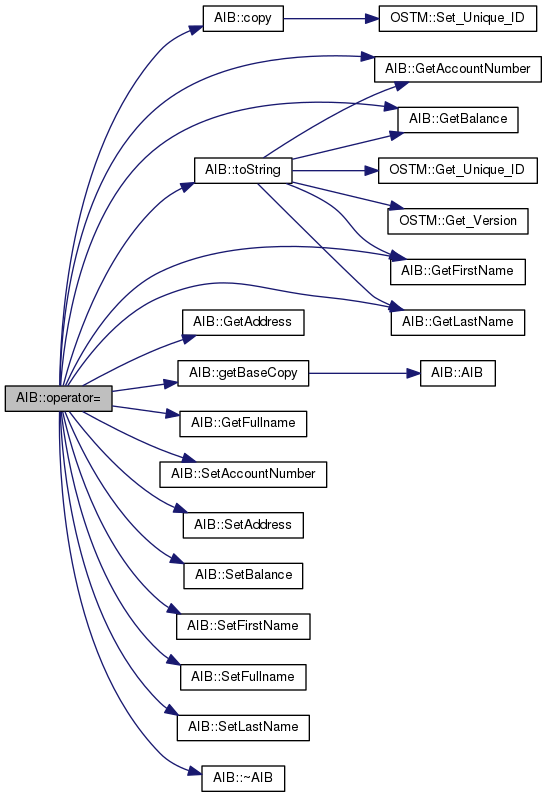
\includegraphics[width=350pt]{class_a_i_b_a77b6f74ea3ef39cb1ccb916db7a48740_a77b6f74ea3ef39cb1ccb916db7a48740_cgraph}
\end{center}
\end{figure}


\index{A\+IB@{A\+IB}!Set\+Account\+Number@{Set\+Account\+Number}}
\index{Set\+Account\+Number@{Set\+Account\+Number}!A\+IB@{A\+IB}}
\paragraph[{\texorpdfstring{Set\+Account\+Number(int account\+Number)}{SetAccountNumber(int accountNumber)}}]{\setlength{\rightskip}{0pt plus 5cm}void A\+I\+B\+::\+Set\+Account\+Number (
\begin{DoxyParamCaption}
\item[{int}]{account\+Number}
\end{DoxyParamCaption}
)\hspace{0.3cm}{\ttfamily [virtual]}}\hypertarget{class_a_i_b_ae582677d2d890f1728dedb9f43965df6_ae582677d2d890f1728dedb9f43965df6}{}\label{class_a_i_b_ae582677d2d890f1728dedb9f43965df6_ae582677d2d890f1728dedb9f43965df6}


Set\+Account\+Number setter for account\+Number private field. 



Reimplemented from \hyperlink{class_b_a_n_k_a9d8fb8bde35d63eca7e9f87d22b45752_a9d8fb8bde35d63eca7e9f87d22b45752}{B\+A\+NK}.



Definition at line \hyperlink{_a_i_b_8cpp_source_l00090}{90} of file \hyperlink{_a_i_b_8cpp_source}{A\+I\+B.\+cpp}.



References \hyperlink{_a_i_b_8h_source_l00123}{account\+Number}.



Referenced by \hyperlink{_a_i_b_8h_source_l00078}{operator=()}.


\begin{DoxyCode}
00090                                             \{
00091     this->\hyperlink{class_a_i_b_aafc08efeec5b8c800c32ee32f20603a7_aafc08efeec5b8c800c32ee32f20603a7}{accountNumber} = \hyperlink{class_a_i_b_aafc08efeec5b8c800c32ee32f20603a7_aafc08efeec5b8c800c32ee32f20603a7}{accountNumber};
00092 \}
\end{DoxyCode}


Here is the caller graph for this function\+:\nopagebreak
\begin{figure}[H]
\begin{center}
\leavevmode
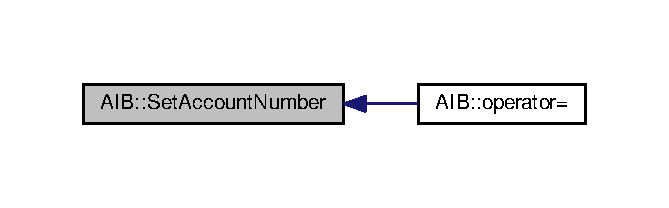
\includegraphics[width=321pt]{class_a_i_b_ae582677d2d890f1728dedb9f43965df6_ae582677d2d890f1728dedb9f43965df6_icgraph}
\end{center}
\end{figure}


\index{A\+IB@{A\+IB}!Set\+Address@{Set\+Address}}
\index{Set\+Address@{Set\+Address}!A\+IB@{A\+IB}}
\paragraph[{\texorpdfstring{Set\+Address(std\+::string address)}{SetAddress(std::string address)}}]{\setlength{\rightskip}{0pt plus 5cm}void A\+I\+B\+::\+Set\+Address (
\begin{DoxyParamCaption}
\item[{std\+::string}]{address}
\end{DoxyParamCaption}
)\hspace{0.3cm}{\ttfamily [virtual]}}\hypertarget{class_a_i_b_ab5fd22fbbc0ea75a022aaeb7174fc450_ab5fd22fbbc0ea75a022aaeb7174fc450}{}\label{class_a_i_b_ab5fd22fbbc0ea75a022aaeb7174fc450_ab5fd22fbbc0ea75a022aaeb7174fc450}


Set\+Address setter for address private field. 



Reimplemented from \hyperlink{class_b_a_n_k_a52ad99454b2059d44967868157208393_a52ad99454b2059d44967868157208393}{B\+A\+NK}.



Definition at line \hyperlink{_a_i_b_8cpp_source_l00066}{66} of file \hyperlink{_a_i_b_8cpp_source}{A\+I\+B.\+cpp}.



References \hyperlink{_a_i_b_8h_source_l00131}{address}.



Referenced by \hyperlink{_a_i_b_8h_source_l00078}{operator=()}.


\begin{DoxyCode}
00066                                       \{
00067     this->\hyperlink{class_a_i_b_ae6a67cc33d1e5fa83a52a238e45ca3dc_ae6a67cc33d1e5fa83a52a238e45ca3dc}{address} = \hyperlink{class_a_i_b_ae6a67cc33d1e5fa83a52a238e45ca3dc_ae6a67cc33d1e5fa83a52a238e45ca3dc}{address};
00068 \}
\end{DoxyCode}


Here is the caller graph for this function\+:\nopagebreak
\begin{figure}[H]
\begin{center}
\leavevmode
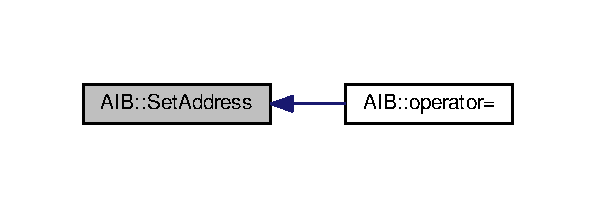
\includegraphics[width=286pt]{class_a_i_b_ab5fd22fbbc0ea75a022aaeb7174fc450_ab5fd22fbbc0ea75a022aaeb7174fc450_icgraph}
\end{center}
\end{figure}


\index{A\+IB@{A\+IB}!Set\+Balance@{Set\+Balance}}
\index{Set\+Balance@{Set\+Balance}!A\+IB@{A\+IB}}
\paragraph[{\texorpdfstring{Set\+Balance(double balance)}{SetBalance(double balance)}}]{\setlength{\rightskip}{0pt plus 5cm}void A\+I\+B\+::\+Set\+Balance (
\begin{DoxyParamCaption}
\item[{double}]{balance}
\end{DoxyParamCaption}
)\hspace{0.3cm}{\ttfamily [virtual]}}\hypertarget{class_a_i_b_ac286e13b8cf985bc88ce356b0eaada81_ac286e13b8cf985bc88ce356b0eaada81}{}\label{class_a_i_b_ac286e13b8cf985bc88ce356b0eaada81_ac286e13b8cf985bc88ce356b0eaada81}


Set\+Balance setter for balance private field. 



Reimplemented from \hyperlink{class_b_a_n_k_ae3e45b407bf8ec7175662442ea24b7c0_ae3e45b407bf8ec7175662442ea24b7c0}{B\+A\+NK}.



Definition at line \hyperlink{_a_i_b_8cpp_source_l00078}{78} of file \hyperlink{_a_i_b_8cpp_source}{A\+I\+B.\+cpp}.



References \hyperlink{_a_i_b_8h_source_l00127}{balance}.



Referenced by \hyperlink{_a_i_b_8h_source_l00078}{operator=()}.


\begin{DoxyCode}
00078                                    \{
00079     this->\hyperlink{class_a_i_b_a3c8d637bd997c1f062d844a88e2559ba_a3c8d637bd997c1f062d844a88e2559ba}{balance} = \hyperlink{class_a_i_b_a3c8d637bd997c1f062d844a88e2559ba_a3c8d637bd997c1f062d844a88e2559ba}{balance};
00080 \}
\end{DoxyCode}


Here is the caller graph for this function\+:\nopagebreak
\begin{figure}[H]
\begin{center}
\leavevmode
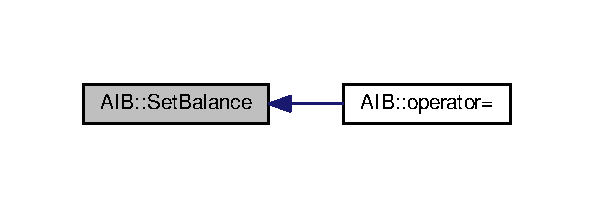
\includegraphics[width=285pt]{class_a_i_b_ac286e13b8cf985bc88ce356b0eaada81_ac286e13b8cf985bc88ce356b0eaada81_icgraph}
\end{center}
\end{figure}


\index{A\+IB@{A\+IB}!Set\+First\+Name@{Set\+First\+Name}}
\index{Set\+First\+Name@{Set\+First\+Name}!A\+IB@{A\+IB}}
\paragraph[{\texorpdfstring{Set\+First\+Name(std\+::string first\+Name)}{SetFirstName(std::string firstName)}}]{\setlength{\rightskip}{0pt plus 5cm}void A\+I\+B\+::\+Set\+First\+Name (
\begin{DoxyParamCaption}
\item[{std\+::string}]{first\+Name}
\end{DoxyParamCaption}
)\hspace{0.3cm}{\ttfamily [virtual]}}\hypertarget{class_a_i_b_a671e44bdbf1286d97d7a22295177dd2e_a671e44bdbf1286d97d7a22295177dd2e}{}\label{class_a_i_b_a671e44bdbf1286d97d7a22295177dd2e_a671e44bdbf1286d97d7a22295177dd2e}


Set\+First\+Name setter for first\+Name private field. 



Reimplemented from \hyperlink{class_b_a_n_k_a547cb9f21be894f045bb3cec6b12525c_a547cb9f21be894f045bb3cec6b12525c}{B\+A\+NK}.



Definition at line \hyperlink{_a_i_b_8cpp_source_l00114}{114} of file \hyperlink{_a_i_b_8cpp_source}{A\+I\+B.\+cpp}.



References \hyperlink{_a_i_b_8h_source_l00115}{first\+Name}.



Referenced by \hyperlink{_a_i_b_8h_source_l00078}{operator=()}.


\begin{DoxyCode}
00114                                           \{
00115     this->\hyperlink{class_a_i_b_a869f72057cb63ebf0cfd257069e15c7c_a869f72057cb63ebf0cfd257069e15c7c}{firstName} = \hyperlink{class_a_i_b_a869f72057cb63ebf0cfd257069e15c7c_a869f72057cb63ebf0cfd257069e15c7c}{firstName};
00116 \}
\end{DoxyCode}


Here is the caller graph for this function\+:\nopagebreak
\begin{figure}[H]
\begin{center}
\leavevmode
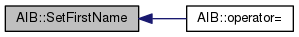
\includegraphics[width=296pt]{class_a_i_b_a671e44bdbf1286d97d7a22295177dd2e_a671e44bdbf1286d97d7a22295177dd2e_icgraph}
\end{center}
\end{figure}


\index{A\+IB@{A\+IB}!Set\+Fullname@{Set\+Fullname}}
\index{Set\+Fullname@{Set\+Fullname}!A\+IB@{A\+IB}}
\paragraph[{\texorpdfstring{Set\+Fullname(std\+::string fullname)}{SetFullname(std::string fullname)}}]{\setlength{\rightskip}{0pt plus 5cm}void A\+I\+B\+::\+Set\+Fullname (
\begin{DoxyParamCaption}
\item[{std\+::string}]{fullname}
\end{DoxyParamCaption}
)\hspace{0.3cm}{\ttfamily [virtual]}}\hypertarget{class_a_i_b_a03def15426e627042951369ea18b97f6_a03def15426e627042951369ea18b97f6}{}\label{class_a_i_b_a03def15426e627042951369ea18b97f6_a03def15426e627042951369ea18b97f6}


Set\+Fullname setter for fullname private field. 



Reimplemented from \hyperlink{class_b_a_n_k_a8845dbfc7ddfbc2e0c0efda561a70ec3_a8845dbfc7ddfbc2e0c0efda561a70ec3}{B\+A\+NK}.



Definition at line \hyperlink{_a_i_b_8cpp_source_l00126}{126} of file \hyperlink{_a_i_b_8cpp_source}{A\+I\+B.\+cpp}.



References \hyperlink{_a_i_b_8h_source_l00111}{fullname}.



Referenced by \hyperlink{_a_i_b_8h_source_l00078}{operator=()}.


\begin{DoxyCode}
00126                                         \{
00127     this->\hyperlink{class_a_i_b_a818b0cc283af23127c067fb3fc751058_a818b0cc283af23127c067fb3fc751058}{fullname} = \hyperlink{class_a_i_b_a818b0cc283af23127c067fb3fc751058_a818b0cc283af23127c067fb3fc751058}{fullname};
00128 \}
\end{DoxyCode}


Here is the caller graph for this function\+:\nopagebreak
\begin{figure}[H]
\begin{center}
\leavevmode
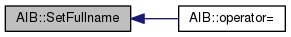
\includegraphics[width=290pt]{class_a_i_b_a03def15426e627042951369ea18b97f6_a03def15426e627042951369ea18b97f6_icgraph}
\end{center}
\end{figure}


\index{A\+IB@{A\+IB}!Set\+Last\+Name@{Set\+Last\+Name}}
\index{Set\+Last\+Name@{Set\+Last\+Name}!A\+IB@{A\+IB}}
\paragraph[{\texorpdfstring{Set\+Last\+Name(std\+::string last\+Name)}{SetLastName(std::string lastName)}}]{\setlength{\rightskip}{0pt plus 5cm}void A\+I\+B\+::\+Set\+Last\+Name (
\begin{DoxyParamCaption}
\item[{std\+::string}]{last\+Name}
\end{DoxyParamCaption}
)\hspace{0.3cm}{\ttfamily [virtual]}}\hypertarget{class_a_i_b_afe4e3c7b481bf87437968dde2cc75882_afe4e3c7b481bf87437968dde2cc75882}{}\label{class_a_i_b_afe4e3c7b481bf87437968dde2cc75882_afe4e3c7b481bf87437968dde2cc75882}


Set\+Last\+Name setter for last\+Name private field. 



Reimplemented from \hyperlink{class_b_a_n_k_a2dc1b7664f9e3b005cb33e71b2ba42ee_a2dc1b7664f9e3b005cb33e71b2ba42ee}{B\+A\+NK}.



Definition at line \hyperlink{_a_i_b_8cpp_source_l00102}{102} of file \hyperlink{_a_i_b_8cpp_source}{A\+I\+B.\+cpp}.



References \hyperlink{_a_i_b_8h_source_l00119}{last\+Name}.



Referenced by \hyperlink{_a_i_b_8h_source_l00078}{operator=()}.


\begin{DoxyCode}
00102                                         \{
00103     this->\hyperlink{class_a_i_b_ace7b8b648d1b44b7ee2f4be002952b7a_ace7b8b648d1b44b7ee2f4be002952b7a}{lastName} = \hyperlink{class_a_i_b_ace7b8b648d1b44b7ee2f4be002952b7a_ace7b8b648d1b44b7ee2f4be002952b7a}{lastName};
00104 \}
\end{DoxyCode}


Here is the caller graph for this function\+:\nopagebreak
\begin{figure}[H]
\begin{center}
\leavevmode
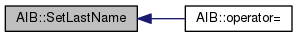
\includegraphics[width=295pt]{class_a_i_b_afe4e3c7b481bf87437968dde2cc75882_afe4e3c7b481bf87437968dde2cc75882_icgraph}
\end{center}
\end{figure}


\index{A\+IB@{A\+IB}!to\+String@{to\+String}}
\index{to\+String@{to\+String}!A\+IB@{A\+IB}}
\paragraph[{\texorpdfstring{to\+String()}{toString()}}]{\setlength{\rightskip}{0pt plus 5cm}void A\+I\+B\+::to\+String (
\begin{DoxyParamCaption}
{}
\end{DoxyParamCaption}
)\hspace{0.3cm}{\ttfamily [virtual]}}\hypertarget{class_a_i_b_aff0f0a0db75a17efec4bd500b888232d_aff0f0a0db75a17efec4bd500b888232d}{}\label{class_a_i_b_aff0f0a0db75a17efec4bd500b888232d_aff0f0a0db75a17efec4bd500b888232d}


to\+String function, displays the object values in formatted way 



Reimplemented from \hyperlink{class_o_s_t_m_a513396a115f2987fd07c203309ae8a59_a513396a115f2987fd07c203309ae8a59}{O\+S\+TM}.



Definition at line \hyperlink{_a_i_b_8cpp_source_l00059}{59} of file \hyperlink{_a_i_b_8cpp_source}{A\+I\+B.\+cpp}.



References \hyperlink{_o_s_t_m_8cpp_source_l00082}{O\+S\+T\+M\+::\+Get\+\_\+\+Unique\+\_\+\+I\+D()}, \hyperlink{_o_s_t_m_8cpp_source_l00100}{O\+S\+T\+M\+::\+Get\+\_\+\+Version()}, \hyperlink{_a_i_b_8cpp_source_l00096}{Get\+Account\+Number()}, \hyperlink{_a_i_b_8cpp_source_l00084}{Get\+Balance()}, \hyperlink{_a_i_b_8cpp_source_l00120}{Get\+First\+Name()}, and \hyperlink{_a_i_b_8cpp_source_l00108}{Get\+Last\+Name()}.



Referenced by \hyperlink{_a_i_b_8h_source_l00078}{operator=()}.


\begin{DoxyCode}
00060 \{
00061     std::cout << \textcolor{stringliteral}{"\(\backslash\)nAIB BANK"} << \textcolor{stringliteral}{"\(\backslash\)nUnique ID : "} << this->\hyperlink{class_o_s_t_m_a5a01a8b98d16b1d1904ecf9356e7b71d_a5a01a8b98d16b1d1904ecf9356e7b71d}{Get\_Unique\_ID}() << \textcolor{stringliteral}{"\(\backslash\)nInt account :
       "} << this->\hyperlink{class_a_i_b_aef34bfbf20d767114e05b8b532cab777_aef34bfbf20d767114e05b8b532cab777}{GetAccountNumber}() << \textcolor{stringliteral}{"\(\backslash\)nDouble value : "} << this->
      \hyperlink{class_a_i_b_ac75087ae73c308bd946e47a71dc85b86_ac75087ae73c308bd946e47a71dc85b86}{GetBalance}() << \textcolor{stringliteral}{"\(\backslash\)nFirst name: "} << this->\hyperlink{class_a_i_b_aa0833919c1c211481560cd88cb5b381b_aa0833919c1c211481560cd88cb5b381b}{GetFirstName}() << \textcolor{stringliteral}{"\(\backslash\)nLast name : "} << 
      this->\hyperlink{class_a_i_b_a1b09db7268734beeaf6a9e7e9d8feb02_a1b09db7268734beeaf6a9e7e9d8feb02}{GetLastName}()  << \textcolor{stringliteral}{"\(\backslash\)nVersion number : "} << this->\hyperlink{class_o_s_t_m_a1f1db9d482f22c8e7caa17dfb340626b_a1f1db9d482f22c8e7caa17dfb340626b}{Get\_Version}() << std::endl;
00062 \}
\end{DoxyCode}


Here is the call graph for this function\+:\nopagebreak
\begin{figure}[H]
\begin{center}
\leavevmode
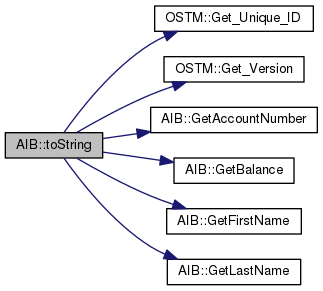
\includegraphics[width=314pt]{class_a_i_b_aff0f0a0db75a17efec4bd500b888232d_aff0f0a0db75a17efec4bd500b888232d_cgraph}
\end{center}
\end{figure}




Here is the caller graph for this function\+:\nopagebreak
\begin{figure}[H]
\begin{center}
\leavevmode
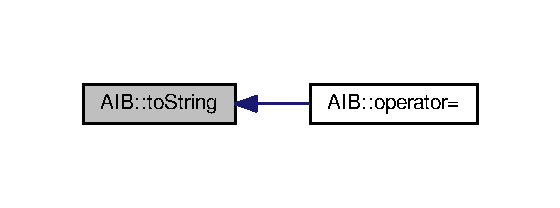
\includegraphics[width=269pt]{class_a_i_b_aff0f0a0db75a17efec4bd500b888232d_aff0f0a0db75a17efec4bd500b888232d_icgraph}
\end{center}
\end{figure}




\subsubsection{Member Data Documentation}
\index{A\+IB@{A\+IB}!account\+Number@{account\+Number}}
\index{account\+Number@{account\+Number}!A\+IB@{A\+IB}}
\paragraph[{\texorpdfstring{account\+Number}{accountNumber}}]{\setlength{\rightskip}{0pt plus 5cm}int A\+I\+B\+::account\+Number\hspace{0.3cm}{\ttfamily [private]}}\hypertarget{class_a_i_b_aafc08efeec5b8c800c32ee32f20603a7_aafc08efeec5b8c800c32ee32f20603a7}{}\label{class_a_i_b_aafc08efeec5b8c800c32ee32f20603a7_aafc08efeec5b8c800c32ee32f20603a7}
account\+Number int object private filed 

Definition at line \hyperlink{_a_i_b_8h_source_l00123}{123} of file \hyperlink{_a_i_b_8h_source}{A\+I\+B.\+h}.



Referenced by \hyperlink{_a_i_b_8h_source_l00028}{A\+I\+B()}, \hyperlink{_a_i_b_8cpp_source_l00096}{Get\+Account\+Number()}, \hyperlink{_a_i_b_8h_source_l00078}{operator=()}, and \hyperlink{_a_i_b_8cpp_source_l00090}{Set\+Account\+Number()}.

\index{A\+IB@{A\+IB}!address@{address}}
\index{address@{address}!A\+IB@{A\+IB}}
\paragraph[{\texorpdfstring{address}{address}}]{\setlength{\rightskip}{0pt plus 5cm}std\+::string A\+I\+B\+::address\hspace{0.3cm}{\ttfamily [private]}}\hypertarget{class_a_i_b_ae6a67cc33d1e5fa83a52a238e45ca3dc_ae6a67cc33d1e5fa83a52a238e45ca3dc}{}\label{class_a_i_b_ae6a67cc33d1e5fa83a52a238e45ca3dc_ae6a67cc33d1e5fa83a52a238e45ca3dc}
address string object private filed 

Definition at line \hyperlink{_a_i_b_8h_source_l00131}{131} of file \hyperlink{_a_i_b_8h_source}{A\+I\+B.\+h}.



Referenced by \hyperlink{_a_i_b_8h_source_l00028}{A\+I\+B()}, \hyperlink{_a_i_b_8cpp_source_l00072}{Get\+Address()}, \hyperlink{_a_i_b_8h_source_l00078}{operator=()}, and \hyperlink{_a_i_b_8cpp_source_l00066}{Set\+Address()}.

\index{A\+IB@{A\+IB}!balance@{balance}}
\index{balance@{balance}!A\+IB@{A\+IB}}
\paragraph[{\texorpdfstring{balance}{balance}}]{\setlength{\rightskip}{0pt plus 5cm}double A\+I\+B\+::balance\hspace{0.3cm}{\ttfamily [private]}}\hypertarget{class_a_i_b_a3c8d637bd997c1f062d844a88e2559ba_a3c8d637bd997c1f062d844a88e2559ba}{}\label{class_a_i_b_a3c8d637bd997c1f062d844a88e2559ba_a3c8d637bd997c1f062d844a88e2559ba}
balance double object private filed 

Definition at line \hyperlink{_a_i_b_8h_source_l00127}{127} of file \hyperlink{_a_i_b_8h_source}{A\+I\+B.\+h}.



Referenced by \hyperlink{_a_i_b_8h_source_l00028}{A\+I\+B()}, \hyperlink{_a_i_b_8cpp_source_l00084}{Get\+Balance()}, \hyperlink{_a_i_b_8h_source_l00078}{operator=()}, and \hyperlink{_a_i_b_8cpp_source_l00078}{Set\+Balance()}.

\index{A\+IB@{A\+IB}!first\+Name@{first\+Name}}
\index{first\+Name@{first\+Name}!A\+IB@{A\+IB}}
\paragraph[{\texorpdfstring{first\+Name}{firstName}}]{\setlength{\rightskip}{0pt plus 5cm}std\+::string A\+I\+B\+::first\+Name\hspace{0.3cm}{\ttfamily [private]}}\hypertarget{class_a_i_b_a869f72057cb63ebf0cfd257069e15c7c_a869f72057cb63ebf0cfd257069e15c7c}{}\label{class_a_i_b_a869f72057cb63ebf0cfd257069e15c7c_a869f72057cb63ebf0cfd257069e15c7c}
first\+Name string object private filed 

Definition at line \hyperlink{_a_i_b_8h_source_l00115}{115} of file \hyperlink{_a_i_b_8h_source}{A\+I\+B.\+h}.



Referenced by \hyperlink{_a_i_b_8h_source_l00028}{A\+I\+B()}, \hyperlink{_a_i_b_8cpp_source_l00120}{Get\+First\+Name()}, \hyperlink{_a_i_b_8h_source_l00078}{operator=()}, and \hyperlink{_a_i_b_8cpp_source_l00114}{Set\+First\+Name()}.

\index{A\+IB@{A\+IB}!fullname@{fullname}}
\index{fullname@{fullname}!A\+IB@{A\+IB}}
\paragraph[{\texorpdfstring{fullname}{fullname}}]{\setlength{\rightskip}{0pt plus 5cm}std\+::string A\+I\+B\+::fullname\hspace{0.3cm}{\ttfamily [private]}}\hypertarget{class_a_i_b_a818b0cc283af23127c067fb3fc751058_a818b0cc283af23127c067fb3fc751058}{}\label{class_a_i_b_a818b0cc283af23127c067fb3fc751058_a818b0cc283af23127c067fb3fc751058}
fullname string object private filed 

Definition at line \hyperlink{_a_i_b_8h_source_l00111}{111} of file \hyperlink{_a_i_b_8h_source}{A\+I\+B.\+h}.



Referenced by \hyperlink{_a_i_b_8h_source_l00028}{A\+I\+B()}, \hyperlink{_a_i_b_8cpp_source_l00132}{Get\+Fullname()}, \hyperlink{_a_i_b_8h_source_l00078}{operator=()}, and \hyperlink{_a_i_b_8cpp_source_l00126}{Set\+Fullname()}.

\index{A\+IB@{A\+IB}!last\+Name@{last\+Name}}
\index{last\+Name@{last\+Name}!A\+IB@{A\+IB}}
\paragraph[{\texorpdfstring{last\+Name}{lastName}}]{\setlength{\rightskip}{0pt plus 5cm}std\+::string A\+I\+B\+::last\+Name\hspace{0.3cm}{\ttfamily [private]}}\hypertarget{class_a_i_b_ace7b8b648d1b44b7ee2f4be002952b7a_ace7b8b648d1b44b7ee2f4be002952b7a}{}\label{class_a_i_b_ace7b8b648d1b44b7ee2f4be002952b7a_ace7b8b648d1b44b7ee2f4be002952b7a}
last\+Name string object private filed 

Definition at line \hyperlink{_a_i_b_8h_source_l00119}{119} of file \hyperlink{_a_i_b_8h_source}{A\+I\+B.\+h}.



Referenced by \hyperlink{_a_i_b_8h_source_l00028}{A\+I\+B()}, \hyperlink{_a_i_b_8cpp_source_l00108}{Get\+Last\+Name()}, \hyperlink{_a_i_b_8h_source_l00078}{operator=()}, and \hyperlink{_a_i_b_8cpp_source_l00102}{Set\+Last\+Name()}.



The documentation for this class was generated from the following files\+:\begin{DoxyCompactItemize}
\item 
\hyperlink{_a_i_b_8h}{A\+I\+B.\+h}\item 
\hyperlink{_a_i_b_8cpp}{A\+I\+B.\+cpp}\end{DoxyCompactItemize}

\section{B\+A\+NK Class Reference}
\label{class_b_a_n_k}\index{B\+A\+NK@{B\+A\+NK}}


{\ttfamily \#include $<$B\+A\+N\+K.\+h$>$}

Inheritance diagram for B\+A\+NK\+:\begin{figure}[H]
\begin{center}
\leavevmode
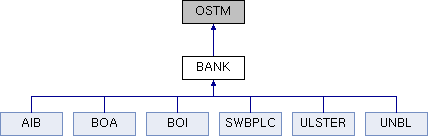
\includegraphics[height=3.000000cm]{class_b_a_n_k}
\end{center}
\end{figure}
\subsection*{Public Member Functions}
\begin{DoxyCompactItemize}
\item 
{\bf B\+A\+NK} ()
\item 
{\bf B\+A\+NK} (int \+\_\+version, int \+\_\+unique\+\_\+id)
\item 
{\bf B\+A\+NK} (const {\bf B\+A\+NK} \&orig)
\item 
virtual {\bf $\sim$\+B\+A\+NK} ()
\item 
virtual void {\bfseries Set\+Address} (std\+::string address)\label{class_b_a_n_k_a52ad99454b2059d44967868157208393}

\item 
virtual std\+::string {\bfseries Get\+Address} () const \label{class_b_a_n_k_a358741f647f9494026e02fd3fd27cde6}

\item 
virtual void {\bfseries Set\+Balance} (double balance)\label{class_b_a_n_k_ae3e45b407bf8ec7175662442ea24b7c0}

\item 
virtual double {\bfseries Get\+Balance} () const \label{class_b_a_n_k_a7ac46c74859cebdc933cb27e148d18b1}

\item 
virtual void {\bfseries Set\+Account\+Number} (int account\+Number)\label{class_b_a_n_k_a9d8fb8bde35d63eca7e9f87d22b45752}

\item 
virtual int {\bfseries Get\+Account\+Number} () const \label{class_b_a_n_k_a62adf3cea60d863a4a10eeee485fa1aa}

\item 
virtual void {\bfseries Set\+Last\+Name} (std\+::string last\+Name)\label{class_b_a_n_k_a2dc1b7664f9e3b005cb33e71b2ba42ee}

\item 
virtual std\+::string {\bfseries Get\+Last\+Name} () const \label{class_b_a_n_k_a4612063ec2bfd6d883a77a0d3697af90}

\item 
virtual void {\bfseries Set\+First\+Name} (std\+::string first\+Name)\label{class_b_a_n_k_a547cb9f21be894f045bb3cec6b12525c}

\item 
virtual std\+::string {\bfseries Get\+First\+Name} () const \label{class_b_a_n_k_ad0ba1c785c67e7d4760dc8776f3d4bca}

\item 
virtual void {\bfseries Set\+Fullname} (std\+::string fullname)\label{class_b_a_n_k_a8845dbfc7ddfbc2e0c0efda561a70ec3}

\item 
virtual std\+::string {\bfseries Get\+Fullname} () const \label{class_b_a_n_k_aa1528c533bf6389bc8d7f3eeca114bab}

\end{DoxyCompactItemize}


\subsection{Detailed Description}
\doxyref{B\+A\+NK}{p.}{class_b_a_n_k} inherit from the \doxyref{O\+S\+TM}{p.}{class_o_s_t_m} library. It is declares the common functions in the child classes as a virtual function. 

Definition at line 16 of file B\+A\+N\+K.\+h.



\subsection{Constructor \& Destructor Documentation}
\index{B\+A\+NK@{B\+A\+NK}!B\+A\+NK@{B\+A\+NK}}
\index{B\+A\+NK@{B\+A\+NK}!B\+A\+NK@{B\+A\+NK}}
\subsubsection[{B\+A\+N\+K()}]{\setlength{\rightskip}{0pt plus 5cm}B\+A\+N\+K\+::\+B\+A\+NK (
\begin{DoxyParamCaption}
{}
\end{DoxyParamCaption}
)\hspace{0.3cm}{\ttfamily [inline]}}\label{class_b_a_n_k_a0bc938356cebff14fb0560264abe5a34}
Constructor 

Definition at line 23 of file B\+A\+N\+K.\+h.

\index{B\+A\+NK@{B\+A\+NK}!B\+A\+NK@{B\+A\+NK}}
\index{B\+A\+NK@{B\+A\+NK}!B\+A\+NK@{B\+A\+NK}}
\subsubsection[{B\+A\+N\+K(int \+\_\+version, int \+\_\+unique\+\_\+id)}]{\setlength{\rightskip}{0pt plus 5cm}B\+A\+N\+K\+::\+B\+A\+NK (
\begin{DoxyParamCaption}
\item[{int}]{\+\_\+version, }
\item[{int}]{\+\_\+unique\+\_\+id}
\end{DoxyParamCaption}
)\hspace{0.3cm}{\ttfamily [inline]}}\label{class_b_a_n_k_a7382dd275d8f4f10a8b53ccbc93e1e87}
Custom Constructor 

Definition at line 29 of file B\+A\+N\+K.\+h.

\index{B\+A\+NK@{B\+A\+NK}!B\+A\+NK@{B\+A\+NK}}
\index{B\+A\+NK@{B\+A\+NK}!B\+A\+NK@{B\+A\+NK}}
\subsubsection[{B\+A\+N\+K(const B\+A\+N\+K \&orig)}]{\setlength{\rightskip}{0pt plus 5cm}B\+A\+N\+K\+::\+B\+A\+NK (
\begin{DoxyParamCaption}
\item[{const {\bf B\+A\+NK} \&}]{orig}
\end{DoxyParamCaption}
)}\label{class_b_a_n_k_a4dd657c30039ea00a040e6226c23ccd4}
Copy constructor 

Definition at line 11 of file B\+A\+N\+K.\+cpp.

\index{B\+A\+NK@{B\+A\+NK}!````~B\+A\+NK@{$\sim$\+B\+A\+NK}}
\index{````~B\+A\+NK@{$\sim$\+B\+A\+NK}!B\+A\+NK@{B\+A\+NK}}
\subsubsection[{$\sim$\+B\+A\+N\+K()}]{\setlength{\rightskip}{0pt plus 5cm}B\+A\+N\+K\+::$\sim$\+B\+A\+NK (
\begin{DoxyParamCaption}
{}
\end{DoxyParamCaption}
)\hspace{0.3cm}{\ttfamily [virtual]}}\label{class_b_a_n_k_ad609a1e004efdebab6495d95eced2346}
de-\/constructor 

Definition at line 14 of file B\+A\+N\+K.\+cpp.



The documentation for this class was generated from the following files\+:\begin{DoxyCompactItemize}
\item 
/media/zoltan/\+Data/00\+\_\+2018\+\_\+\+I\+T\+Carlow/00\+\_\+\+Modules/06\+\_\+\+Project/\+Documents/\+Git\+\_\+\+Sync/\+Main Tests for Linux/\+Test01/B\+A\+N\+K.\+h\item 
/media/zoltan/\+Data/00\+\_\+2018\+\_\+\+I\+T\+Carlow/00\+\_\+\+Modules/06\+\_\+\+Project/\+Documents/\+Git\+\_\+\+Sync/\+Main Tests for Linux/\+Test01/B\+A\+N\+K.\+cpp\end{DoxyCompactItemize}

\section{B\+OA Class Reference}
\label{class_b_o_a}\index{B\+OA@{B\+OA}}


{\ttfamily \#include $<$B\+O\+A.\+h$>$}

Inheritance diagram for B\+OA\+:\begin{figure}[H]
\begin{center}
\leavevmode
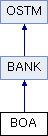
\includegraphics[height=3.000000cm]{class_b_o_a}
\end{center}
\end{figure}
\subsection*{Public Member Functions}
\begin{DoxyCompactItemize}
\item 
{\bf B\+OA} ()
\item 
{\bf B\+OA} (int account\+Number, double balance, std\+::string first\+Name, std\+::string last\+Name, std\+::string address)
\item 
{\bf B\+OA} (std\+::shared\+\_\+ptr$<$ {\bf B\+A\+NK} $>$ obj, int \+\_\+version, int \+\_\+unique\+\_\+id)
\item 
{\bf B\+OA} (const {\bf B\+OA} \&orig)
\item 
{\bf B\+OA} {\bf operator=} (const {\bf B\+OA} \&orig)
\item 
virtual {\bf $\sim$\+B\+OA} ()
\item 
virtual void {\bf copy} (std\+::shared\+\_\+ptr$<$ {\bf O\+S\+TM} $>$ to, std\+::shared\+\_\+ptr$<$ {\bf O\+S\+TM} $>$ from)
\begin{DoxyCompactList}\small\item\em copy function, make deep copy of the object/pointer \end{DoxyCompactList}\item 
virtual std\+::shared\+\_\+ptr$<$ {\bf O\+S\+TM} $>$ {\bf get\+Base\+Copy} (std\+::shared\+\_\+ptr$<$ {\bf O\+S\+TM} $>$ object)
\begin{DoxyCompactList}\small\item\em get\+Base\+Copy function, make deep copy of the object/pointer and Return a new std\+::shared\+\_\+ptr$<$\+B\+A\+N\+K$>$ type object \end{DoxyCompactList}\item 
virtual void {\bf to\+String} ()
\begin{DoxyCompactList}\small\item\em \+\_\+cast, is use to cast bak the std\+::shared\+\_\+ptr$<$\+O\+S\+T\+M$>$ to the required type \end{DoxyCompactList}\item 
virtual void {\bfseries Set\+Address} (std\+::string address)\label{class_b_o_a_a2568c0027af6534bd08dde882e892caf}

\item 
virtual std\+::string {\bfseries Get\+Address} () const \label{class_b_o_a_aa4aa2cf1ef0e876bb7911c00b5374493}

\item 
virtual void {\bfseries Set\+Balance} (double balance)\label{class_b_o_a_a0e06a7b7669b6a26a41b37d68f0a87b8}

\item 
virtual double {\bfseries Get\+Balance} () const \label{class_b_o_a_a07e30b7e5f5f20392b94af7344fd550c}

\item 
virtual void {\bfseries Set\+Account\+Number} (int account\+Number)\label{class_b_o_a_a6b85963680344bd719ab862a50a09588}

\item 
virtual int {\bfseries Get\+Account\+Number} () const \label{class_b_o_a_ad64bd63675f8902153aa6767994f05dc}

\item 
virtual void {\bfseries Set\+Last\+Name} (std\+::string last\+Name)\label{class_b_o_a_a7ea44308c05532cd11ff3ce8f14ea4c2}

\item 
virtual std\+::string {\bfseries Get\+Last\+Name} () const \label{class_b_o_a_a081383edefc1f66b80c3fb8862ab070b}

\item 
virtual void {\bfseries Set\+First\+Name} (std\+::string first\+Name)\label{class_b_o_a_a32fabc2b3acde832f3749696b302a0fe}

\item 
virtual std\+::string {\bfseries Get\+First\+Name} () const \label{class_b_o_a_ae6bb3df4e1fb210610325ffd1985c7c0}

\item 
virtual void {\bfseries Set\+Fullname} (std\+::string fullname)\label{class_b_o_a_a7ff134d56805088f46df8eb6f21a0a45}

\item 
virtual std\+::string {\bfseries Get\+Fullname} () const \label{class_b_o_a_afafa24a20fda93382782cab66a3079ee}

\end{DoxyCompactItemize}


\subsection{Detailed Description}
Inherit from \doxyref{B\+A\+NK}{p.}{class_b_a_n_k} 

Definition at line 18 of file B\+O\+A.\+h.



\subsection{Constructor \& Destructor Documentation}
\index{B\+OA@{B\+OA}!B\+OA@{B\+OA}}
\index{B\+OA@{B\+OA}!B\+OA@{B\+OA}}
\subsubsection[{B\+O\+A()}]{\setlength{\rightskip}{0pt plus 5cm}B\+O\+A\+::\+B\+OA (
\begin{DoxyParamCaption}
{}
\end{DoxyParamCaption}
)\hspace{0.3cm}{\ttfamily [inline]}}\label{class_b_o_a_ad42dc670d422172c9bcf9b3d354c8a3c}
Constructor 

Definition at line 24 of file B\+O\+A.\+h.

\index{B\+OA@{B\+OA}!B\+OA@{B\+OA}}
\index{B\+OA@{B\+OA}!B\+OA@{B\+OA}}
\subsubsection[{B\+O\+A(int account\+Number, double balance, std\+::string first\+Name, std\+::string last\+Name, std\+::string address)}]{\setlength{\rightskip}{0pt plus 5cm}B\+O\+A\+::\+B\+OA (
\begin{DoxyParamCaption}
\item[{int}]{account\+Number, }
\item[{double}]{balance, }
\item[{std\+::string}]{first\+Name, }
\item[{std\+::string}]{last\+Name, }
\item[{std\+::string}]{address}
\end{DoxyParamCaption}
)\hspace{0.3cm}{\ttfamily [inline]}}\label{class_b_o_a_a898c8627b8976bbe1a7d0fc780642b25}
Custom constructor 

Definition at line 35 of file B\+O\+A.\+h.

\index{B\+OA@{B\+OA}!B\+OA@{B\+OA}}
\index{B\+OA@{B\+OA}!B\+OA@{B\+OA}}
\subsubsection[{B\+O\+A(std\+::shared\+\_\+ptr$<$ B\+A\+N\+K $>$ obj, int \+\_\+version, int \+\_\+unique\+\_\+id)}]{\setlength{\rightskip}{0pt plus 5cm}B\+O\+A\+::\+B\+OA (
\begin{DoxyParamCaption}
\item[{std\+::shared\+\_\+ptr$<$ {\bf B\+A\+NK} $>$}]{obj, }
\item[{int}]{\+\_\+version, }
\item[{int}]{\+\_\+unique\+\_\+id}
\end{DoxyParamCaption}
)\hspace{0.3cm}{\ttfamily [inline]}}\label{class_b_o_a_ab87192ed986e601c2eb682ea3745daf0}
Custom constructor, used by the library for deep copying 

Definition at line 46 of file B\+O\+A.\+h.

\index{B\+OA@{B\+OA}!B\+OA@{B\+OA}}
\index{B\+OA@{B\+OA}!B\+OA@{B\+OA}}
\subsubsection[{B\+O\+A(const B\+O\+A \&orig)}]{\setlength{\rightskip}{0pt plus 5cm}B\+O\+A\+::\+B\+OA (
\begin{DoxyParamCaption}
\item[{const {\bf B\+OA} \&}]{orig}
\end{DoxyParamCaption}
)}\label{class_b_o_a_a99ebf22a8d824761dc82e7e191e6f173}
Copy constructor 

Definition at line 12 of file B\+O\+A.\+cpp.

\index{B\+OA@{B\+OA}!````~B\+OA@{$\sim$\+B\+OA}}
\index{````~B\+OA@{$\sim$\+B\+OA}!B\+OA@{B\+OA}}
\subsubsection[{$\sim$\+B\+O\+A()}]{\setlength{\rightskip}{0pt plus 5cm}B\+O\+A\+::$\sim$\+B\+OA (
\begin{DoxyParamCaption}
{}
\end{DoxyParamCaption}
)\hspace{0.3cm}{\ttfamily [virtual]}}\label{class_b_o_a_abe27b17a23ceffc6269dbe6d81de5212}
de-\/constructor 

Definition at line 15 of file B\+O\+A.\+cpp.



\subsection{Member Function Documentation}
\index{B\+OA@{B\+OA}!copy@{copy}}
\index{copy@{copy}!B\+OA@{B\+OA}}
\subsubsection[{copy(std\+::shared\+\_\+ptr$<$ O\+S\+T\+M $>$ to, std\+::shared\+\_\+ptr$<$ O\+S\+T\+M $>$ from)}]{\setlength{\rightskip}{0pt plus 5cm}void B\+O\+A\+::copy (
\begin{DoxyParamCaption}
\item[{std\+::shared\+\_\+ptr$<$ {\bf O\+S\+TM} $>$}]{to, }
\item[{std\+::shared\+\_\+ptr$<$ {\bf O\+S\+TM} $>$}]{from}
\end{DoxyParamCaption}
)\hspace{0.3cm}{\ttfamily [virtual]}}\label{class_b_o_a_a54fbcabb55b22fb72f45986768974403}


copy function, make deep copy of the object/pointer 


\begin{DoxyParams}{Parameters}
{\em obj\+TO} & is a std\+::shared\+\_\+ptr$<$\+B\+A\+N\+K$>$ type object casted back from std\+::shared\+\_\+ptr$<$\+O\+S\+T\+M$>$ \\
\hline
{\em obj\+F\+R\+OM} & is a std\+::shared\+\_\+ptr$<$\+B\+A\+N\+K$>$ type object casted back from std\+::shared\+\_\+ptr$<$\+O\+S\+T\+M$>$ \\
\hline
\end{DoxyParams}


Reimplemented from {\bf O\+S\+TM} \doxyref{}{p.}{class_o_s_t_m_a535d90fced5adbb70312c92f3778e08d}.



Definition at line 34 of file B\+O\+A.\+cpp.

\index{B\+OA@{B\+OA}!get\+Base\+Copy@{get\+Base\+Copy}}
\index{get\+Base\+Copy@{get\+Base\+Copy}!B\+OA@{B\+OA}}
\subsubsection[{get\+Base\+Copy(std\+::shared\+\_\+ptr$<$ O\+S\+T\+M $>$ object)}]{\setlength{\rightskip}{0pt plus 5cm}std\+::shared\+\_\+ptr$<$ {\bf O\+S\+TM} $>$ B\+O\+A\+::get\+Base\+Copy (
\begin{DoxyParamCaption}
\item[{std\+::shared\+\_\+ptr$<$ {\bf O\+S\+TM} $>$}]{object}
\end{DoxyParamCaption}
)\hspace{0.3cm}{\ttfamily [virtual]}}\label{class_b_o_a_a46ace5d3c945a423e93912673cadfad5}


get\+Base\+Copy function, make deep copy of the object/pointer and Return a new std\+::shared\+\_\+ptr$<$\+B\+A\+N\+K$>$ type object 


\begin{DoxyParams}{Parameters}
{\em obj\+TO} & is a \doxyref{B\+A\+NK}{p.}{class_b_a_n_k} type pointer for casting \\
\hline
{\em obj} & is a std\+::shared\+\_\+ptr$<$\+B\+A\+N\+K$>$ return type \\
\hline
\end{DoxyParams}


Reimplemented from {\bf O\+S\+TM} \doxyref{}{p.}{class_o_s_t_m_a0bfa3763bd441407dd6365f42714f94c}.



Definition at line 22 of file B\+O\+A.\+cpp.

\index{B\+OA@{B\+OA}!operator=@{operator=}}
\index{operator=@{operator=}!B\+OA@{B\+OA}}
\subsubsection[{operator=(const B\+O\+A \&orig)}]{\setlength{\rightskip}{0pt plus 5cm}{\bf B\+OA} B\+O\+A\+::operator= (
\begin{DoxyParamCaption}
\item[{const {\bf B\+OA} \&}]{orig}
\end{DoxyParamCaption}
)\hspace{0.3cm}{\ttfamily [inline]}}\label{class_b_o_a_af24b66f0e072b29abbbe5812cab48369}
Operator 

Definition at line 64 of file B\+O\+A.\+h.

\index{B\+OA@{B\+OA}!to\+String@{to\+String}}
\index{to\+String@{to\+String}!B\+OA@{B\+OA}}
\subsubsection[{to\+String()}]{\setlength{\rightskip}{0pt plus 5cm}void B\+O\+A\+::to\+String (
\begin{DoxyParamCaption}
{}
\end{DoxyParamCaption}
)\hspace{0.3cm}{\ttfamily [virtual]}}\label{class_b_o_a_a348df0299997f81bcad0ec034dab0b8d}


\+\_\+cast, is use to cast bak the std\+::shared\+\_\+ptr$<$\+O\+S\+T\+M$>$ to the required type 

to\+String function, displays the object values in formatted way 

Reimplemented from {\bf O\+S\+TM} \doxyref{}{p.}{class_o_s_t_m_a513396a115f2987fd07c203309ae8a59}.



Definition at line 54 of file B\+O\+A.\+cpp.



The documentation for this class was generated from the following files\+:\begin{DoxyCompactItemize}
\item 
/media/zoltan/\+Data/00\+\_\+2018\+\_\+\+I\+T\+Carlow/00\+\_\+\+Modules/06\+\_\+\+Project/\+Documents/\+Git\+\_\+\+Sync/\+Main Tests for Linux/\+Test01/B\+O\+A.\+h\item 
/media/zoltan/\+Data/00\+\_\+2018\+\_\+\+I\+T\+Carlow/00\+\_\+\+Modules/06\+\_\+\+Project/\+Documents/\+Git\+\_\+\+Sync/\+Main Tests for Linux/\+Test01/B\+O\+A.\+cpp\end{DoxyCompactItemize}

\hypertarget{class_b_o_i}{}\subsection{B\+OI Class Reference}
\label{class_b_o_i}\index{B\+OI@{B\+OI}}


{\ttfamily \#include $<$B\+O\+I.\+h$>$}



Inheritance diagram for B\+OI\+:
\nopagebreak
\begin{figure}[H]
\begin{center}
\leavevmode
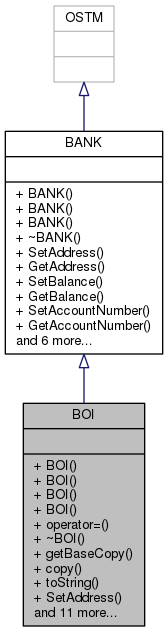
\includegraphics[width=198pt]{class_b_o_i__inherit__graph}
\end{center}
\end{figure}


Collaboration diagram for B\+OI\+:
\nopagebreak
\begin{figure}[H]
\begin{center}
\leavevmode
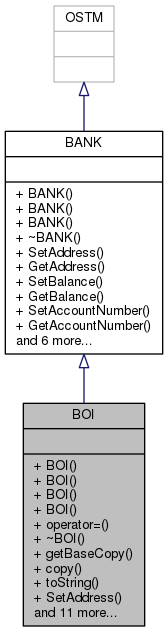
\includegraphics[width=198pt]{class_b_o_i__coll__graph}
\end{center}
\end{figure}
\subsubsection*{Public Member Functions}
\begin{DoxyCompactItemize}
\item 
\hyperlink{class_b_o_i_a6af682a5f199a029681f0cb2b8658706}{B\+OI} ()
\item 
\hyperlink{class_b_o_i_a1807bd07cad08109c974edbb2c32591c}{B\+OI} (int account\+Number, double balance, std\+::string first\+Name, std\+::string last\+Name, std\+::string address)
\item 
\hyperlink{class_b_o_i_ae4263940f8ffdd40d5f01a714b20f791}{B\+OI} (std\+::shared\+\_\+ptr$<$ \hyperlink{class_b_o_i}{B\+OI} $>$ obj, int \+\_\+version, int \+\_\+unique\+\_\+id)
\item 
\hyperlink{class_b_o_i_a7757de8d3ac656871bed4b07d77457ff}{B\+OI} (const \hyperlink{class_b_o_i}{B\+OI} \&orig)
\item 
\hyperlink{class_b_o_i}{B\+OI} \hyperlink{class_b_o_i_a4b4a3976cc13c4d3de0d7ff8882a7af3}{operator=} (const \hyperlink{class_b_o_i}{B\+OI} \&orig)
\item 
virtual \hyperlink{class_b_o_i_a617f46a599129178c6b11b4846759a6c}{$\sim$\+B\+OI} ()
\item 
virtual std\+::shared\+\_\+ptr$<$ O\+S\+TM $>$ \hyperlink{class_b_o_i_ad53ae2918a656793b9d7a670d35ecfa3}{get\+Base\+Copy} (std\+::shared\+\_\+ptr$<$ O\+S\+TM $>$ object)
\begin{DoxyCompactList}\small\item\em get\+Base\+Copy function, make deep copy of the object/pointer and Return a new B\+A\+N\+K$\ast$ type object \end{DoxyCompactList}\item 
virtual void \hyperlink{class_b_o_i_a9ff2d32c25c23a1bea6316f50c3bf677}{copy} (std\+::shared\+\_\+ptr$<$ O\+S\+TM $>$ to, std\+::shared\+\_\+ptr$<$ O\+S\+TM $>$ from)
\begin{DoxyCompactList}\small\item\em copy function, make deep copy of the object/pointer \end{DoxyCompactList}\item 
virtual void \hyperlink{class_b_o_i_ab02a4dd4ebcc5b2abfaca19f2dff2006}{to\+String} ()
\begin{DoxyCompactList}\small\item\em \+\_\+cast, is use to cast bak the std\+::shared\+\_\+ptr$<$\+O\+S\+T\+M$>$ to the required type \end{DoxyCompactList}\item 
virtual void \hyperlink{class_b_o_i_a00c9386c862cf2442968bf7fc30102b3}{Set\+Address} (std\+::string address)
\item 
virtual std\+::string \hyperlink{class_b_o_i_a8920e1f47b22445ba954e86012207462}{Get\+Address} () const 
\item 
virtual void \hyperlink{class_b_o_i_a416667693c10f5e4120eec97a9269348}{Set\+Balance} (double balance)
\item 
virtual double \hyperlink{class_b_o_i_a25b289dece2a1685bb9d1a9332c9be0b}{Get\+Balance} () const 
\item 
virtual void \hyperlink{class_b_o_i_affc9e7e2a36214b3790f250b7108bb65}{Set\+Account\+Number} (int account\+Number)
\item 
virtual int \hyperlink{class_b_o_i_a5b18e1538f3d37835234946cdf9f240f}{Get\+Account\+Number} () const 
\item 
virtual void \hyperlink{class_b_o_i_a663906e9a59ffa970fb928746c01e8af}{Set\+Last\+Name} (std\+::string last\+Name)
\item 
virtual std\+::string \hyperlink{class_b_o_i_a37828f3fa4a32f522966e2cad90eaab2}{Get\+Last\+Name} () const 
\item 
virtual void \hyperlink{class_b_o_i_ae9042f87be085c2cec799981c30d7d19}{Set\+First\+Name} (std\+::string first\+Name)
\item 
virtual std\+::string \hyperlink{class_b_o_i_ab4b9d50c6008a666aa4382def580e7d1}{Get\+First\+Name} () const 
\item 
virtual void \hyperlink{class_b_o_i_a93091f16610f1a1474aea31fd5f81ffd}{Set\+Fullname} (std\+::string fullname)
\item 
virtual std\+::string \hyperlink{class_b_o_i_af56446a377068cd65526e40e8b31b878}{Get\+Fullname} () const 
\end{DoxyCompactItemize}


\subsubsection{Detailed Description}
Inherit from \hyperlink{class_b_a_n_k}{B\+A\+NK} 

Definition at line \hyperlink{_b_o_i_8h_source_l00019}{19} of file \hyperlink{_b_o_i_8h_source}{B\+O\+I.\+h}.



\subsubsection{Constructor \& Destructor Documentation}
\index{B\+OI@{B\+OI}!B\+OI@{B\+OI}}
\index{B\+OI@{B\+OI}!B\+OI@{B\+OI}}
\paragraph[{\texorpdfstring{B\+O\+I()}{BOI()}}]{\setlength{\rightskip}{0pt plus 5cm}B\+O\+I\+::\+B\+OI (
\begin{DoxyParamCaption}
{}
\end{DoxyParamCaption}
)\hspace{0.3cm}{\ttfamily [inline]}}\hypertarget{class_b_o_i_a6af682a5f199a029681f0cb2b8658706}{}\label{class_b_o_i_a6af682a5f199a029681f0cb2b8658706}
Constructor 

Definition at line \hyperlink{_b_o_i_8h_source_l00024}{24} of file \hyperlink{_b_o_i_8h_source}{B\+O\+I.\+h}.



Referenced by \hyperlink{_b_o_i_8h_source_l00049}{B\+O\+I()}, and \hyperlink{_b_o_i_8cpp_source_l00022}{get\+Base\+Copy()}.


\begin{DoxyCode}
00024          : \hyperlink{class_b_a_n_k_a0bc938356cebff14fb0560264abe5a34}{BANK}()
00025     \{
00026         this->accountNumber = 0;
00027         this->balance = 50;
00028         this->firstName = \textcolor{stringliteral}{"Joe"};
00029         this->lastName = \textcolor{stringliteral}{"Blog"};
00030         this->address = \textcolor{stringliteral}{"High street, Carlow"};
00031         this->fullname = firstName + \textcolor{stringliteral}{" "} + lastName;
00032         
00033     \}
\end{DoxyCode}


Here is the caller graph for this function\+:\nopagebreak
\begin{figure}[H]
\begin{center}
\leavevmode
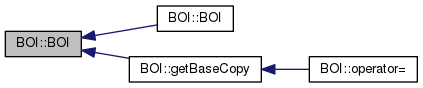
\includegraphics[width=350pt]{class_b_o_i_a6af682a5f199a029681f0cb2b8658706_icgraph}
\end{center}
\end{figure}


\index{B\+OI@{B\+OI}!B\+OI@{B\+OI}}
\index{B\+OI@{B\+OI}!B\+OI@{B\+OI}}
\paragraph[{\texorpdfstring{B\+O\+I(int account\+Number, double balance, std\+::string first\+Name, std\+::string last\+Name, std\+::string address)}{BOI(int accountNumber, double balance, std::string firstName, std::string lastName, std::string address)}}]{\setlength{\rightskip}{0pt plus 5cm}B\+O\+I\+::\+B\+OI (
\begin{DoxyParamCaption}
\item[{int}]{account\+Number, }
\item[{double}]{balance, }
\item[{std\+::string}]{first\+Name, }
\item[{std\+::string}]{last\+Name, }
\item[{std\+::string}]{address}
\end{DoxyParamCaption}
)\hspace{0.3cm}{\ttfamily [inline]}}\hypertarget{class_b_o_i_a1807bd07cad08109c974edbb2c32591c}{}\label{class_b_o_i_a1807bd07cad08109c974edbb2c32591c}
Custom constructor 

Definition at line \hyperlink{_b_o_i_8h_source_l00037}{37} of file \hyperlink{_b_o_i_8h_source}{B\+O\+I.\+h}.


\begin{DoxyCode}
00037                                                                                                       : 
      \hyperlink{class_b_a_n_k_a0bc938356cebff14fb0560264abe5a34}{BANK}()
00038     \{
00039         this->accountNumber = accountNumber;
00040         this->balance = balance;
00041         this->firstName = firstName;
00042         this->lastName = lastName;
00043         this->address = address;
00044         this->fullname = firstName + \textcolor{stringliteral}{" "} + lastName;
00045     \};
\end{DoxyCode}
\index{B\+OI@{B\+OI}!B\+OI@{B\+OI}}
\index{B\+OI@{B\+OI}!B\+OI@{B\+OI}}
\paragraph[{\texorpdfstring{B\+O\+I(std\+::shared\+\_\+ptr$<$ B\+O\+I $>$ obj, int \+\_\+version, int \+\_\+unique\+\_\+id)}{BOI(std::shared_ptr< BOI > obj, int _version, int _unique_id)}}]{\setlength{\rightskip}{0pt plus 5cm}B\+O\+I\+::\+B\+OI (
\begin{DoxyParamCaption}
\item[{std\+::shared\+\_\+ptr$<$ {\bf B\+OI} $>$}]{obj, }
\item[{int}]{\+\_\+version, }
\item[{int}]{\+\_\+unique\+\_\+id}
\end{DoxyParamCaption}
)\hspace{0.3cm}{\ttfamily [inline]}}\hypertarget{class_b_o_i_ae4263940f8ffdd40d5f01a714b20f791}{}\label{class_b_o_i_ae4263940f8ffdd40d5f01a714b20f791}
Custom constructor, used by the library for deep copying 

Definition at line \hyperlink{_b_o_i_8h_source_l00049}{49} of file \hyperlink{_b_o_i_8h_source}{B\+O\+I.\+h}.



References \hyperlink{_b_o_i_8h_source_l00024}{B\+O\+I()}.


\begin{DoxyCode}
00049                                                              : \hyperlink{class_b_a_n_k_a0bc938356cebff14fb0560264abe5a34}{BANK}(\_version, \_unique\_id)
00050     \{
00051         this->accountNumber = obj->GetAccountNumber();
00052         this->balance = obj->GetBalance();
00053         this->firstName = obj->GetFirstName();
00054         this->lastName = obj->GetLastName();
00055         this->address = obj->GetAddress();
00056         this->fullname = obj->GetFirstName() + \textcolor{stringliteral}{" "} + obj->GetLastName(); 
00057     \};
\end{DoxyCode}


Here is the call graph for this function\+:\nopagebreak
\begin{figure}[H]
\begin{center}
\leavevmode
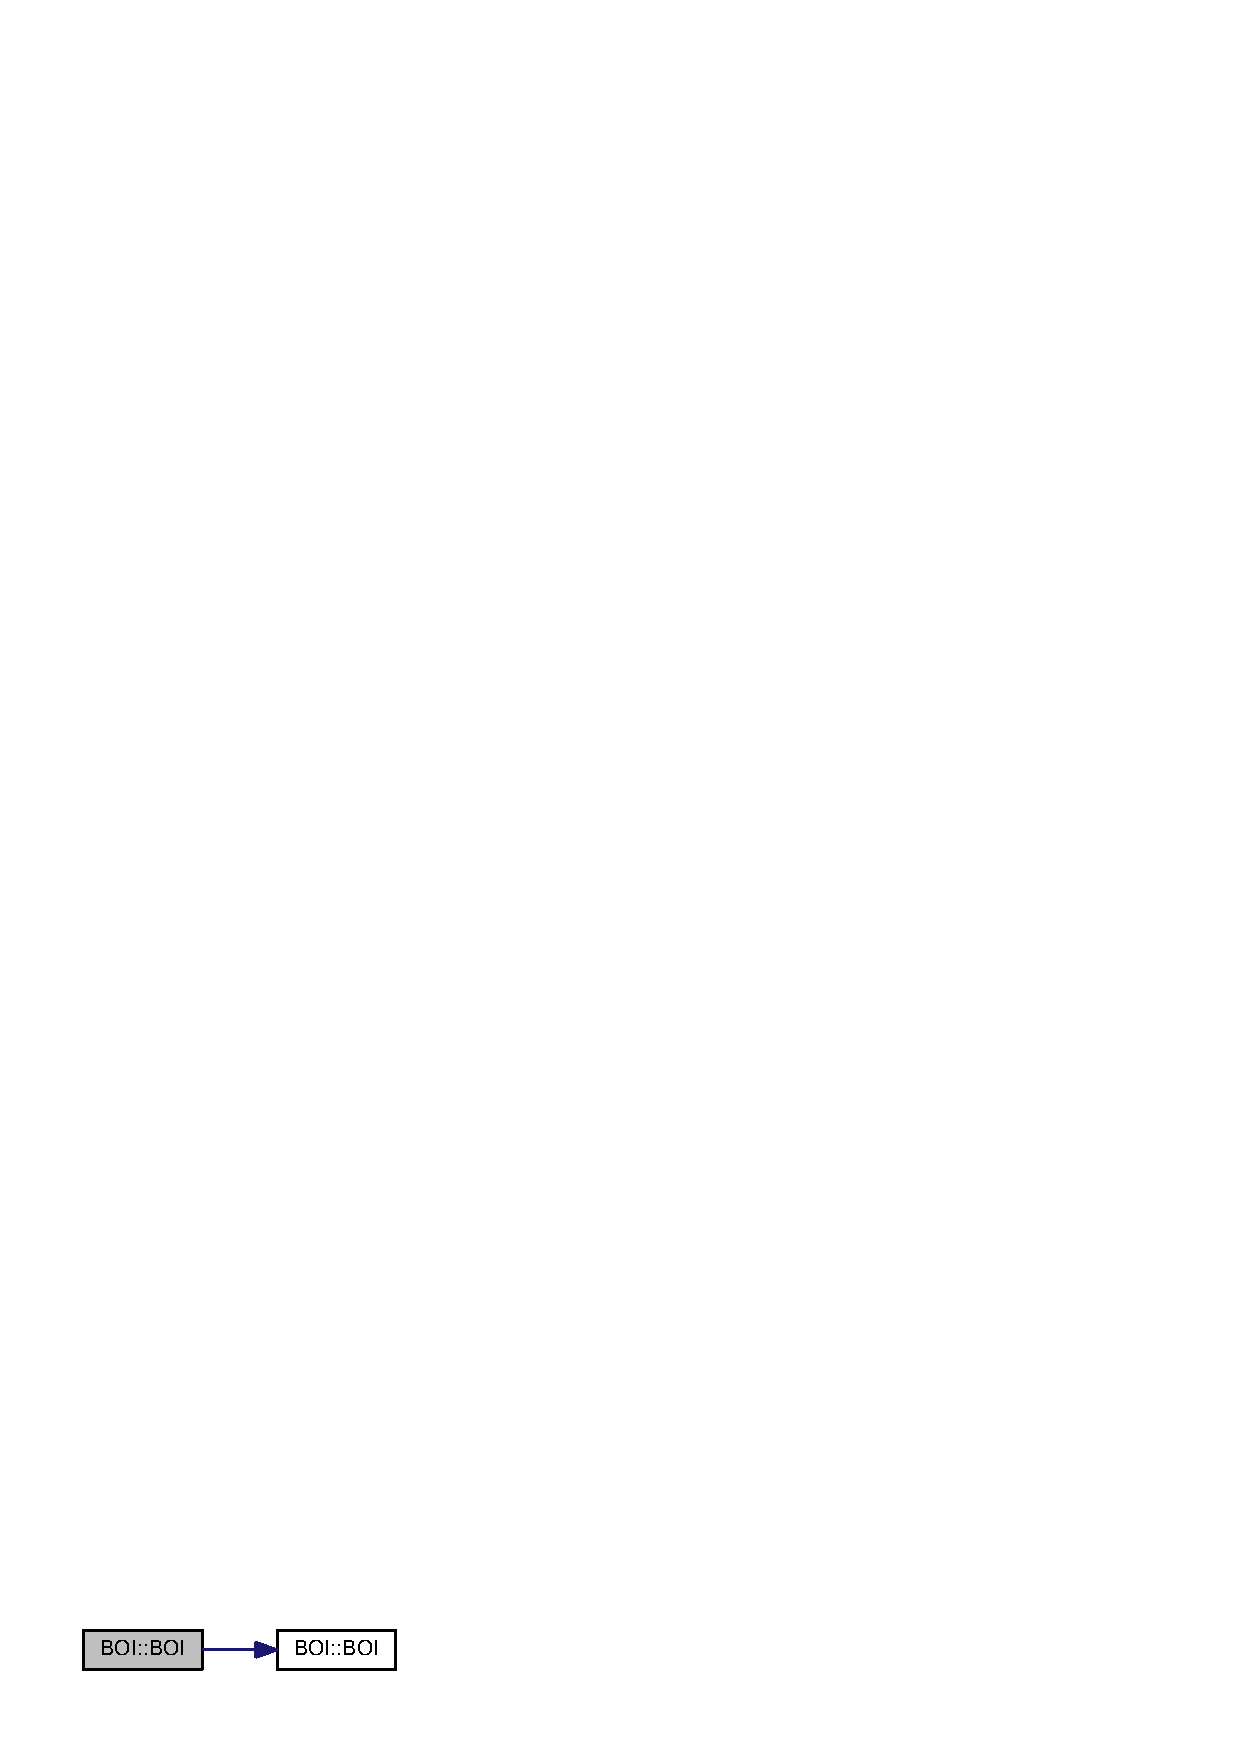
\includegraphics[width=230pt]{class_b_o_i_ae4263940f8ffdd40d5f01a714b20f791_cgraph}
\end{center}
\end{figure}


\index{B\+OI@{B\+OI}!B\+OI@{B\+OI}}
\index{B\+OI@{B\+OI}!B\+OI@{B\+OI}}
\paragraph[{\texorpdfstring{B\+O\+I(const B\+O\+I \&orig)}{BOI(const BOI &orig)}}]{\setlength{\rightskip}{0pt plus 5cm}B\+O\+I\+::\+B\+OI (
\begin{DoxyParamCaption}
\item[{const {\bf B\+OI} \&}]{orig}
\end{DoxyParamCaption}
)}\hypertarget{class_b_o_i_a7757de8d3ac656871bed4b07d77457ff}{}\label{class_b_o_i_a7757de8d3ac656871bed4b07d77457ff}
Copy constructor 

Definition at line \hyperlink{_b_o_i_8cpp_source_l00015}{15} of file \hyperlink{_b_o_i_8cpp_source}{B\+O\+I.\+cpp}.


\begin{DoxyCode}
00015                         \{
00016 \}
\end{DoxyCode}
\index{B\+OI@{B\+OI}!````~B\+OI@{$\sim$\+B\+OI}}
\index{````~B\+OI@{$\sim$\+B\+OI}!B\+OI@{B\+OI}}
\paragraph[{\texorpdfstring{$\sim$\+B\+O\+I()}{~BOI()}}]{\setlength{\rightskip}{0pt plus 5cm}B\+O\+I\+::$\sim$\+B\+OI (
\begin{DoxyParamCaption}
{}
\end{DoxyParamCaption}
)\hspace{0.3cm}{\ttfamily [virtual]}}\hypertarget{class_b_o_i_a617f46a599129178c6b11b4846759a6c}{}\label{class_b_o_i_a617f46a599129178c6b11b4846759a6c}
de-\/constructor 

Definition at line \hyperlink{_b_o_i_8cpp_source_l00012}{12} of file \hyperlink{_b_o_i_8cpp_source}{B\+O\+I.\+cpp}.



Referenced by \hyperlink{_b_o_i_8h_source_l00065}{operator=()}.


\begin{DoxyCode}
00012           \{
00013 \}
\end{DoxyCode}


Here is the caller graph for this function\+:\nopagebreak
\begin{figure}[H]
\begin{center}
\leavevmode
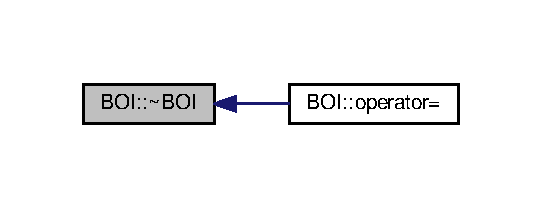
\includegraphics[width=260pt]{class_b_o_i_a617f46a599129178c6b11b4846759a6c_icgraph}
\end{center}
\end{figure}




\subsubsection{Member Function Documentation}
\index{B\+OI@{B\+OI}!copy@{copy}}
\index{copy@{copy}!B\+OI@{B\+OI}}
\paragraph[{\texorpdfstring{copy(std\+::shared\+\_\+ptr$<$ O\+S\+T\+M $>$ to, std\+::shared\+\_\+ptr$<$ O\+S\+T\+M $>$ from)}{copy(std::shared_ptr< OSTM > to, std::shared_ptr< OSTM > from)}}]{\setlength{\rightskip}{0pt plus 5cm}void B\+O\+I\+::copy (
\begin{DoxyParamCaption}
\item[{std\+::shared\+\_\+ptr$<$ O\+S\+TM $>$}]{to, }
\item[{std\+::shared\+\_\+ptr$<$ O\+S\+TM $>$}]{from}
\end{DoxyParamCaption}
)\hspace{0.3cm}{\ttfamily [virtual]}}\hypertarget{class_b_o_i_a9ff2d32c25c23a1bea6316f50c3bf677}{}\label{class_b_o_i_a9ff2d32c25c23a1bea6316f50c3bf677}


copy function, make deep copy of the object/pointer 


\begin{DoxyParams}{Parameters}
{\em obj\+TO} & is a B\+A\+N\+K$\ast$ type object casted back from std\+::shared\+\_\+ptr$<$\+O\+S\+T\+M$>$ \\
\hline
{\em obj\+F\+R\+OM} & is a B\+A\+N\+K$\ast$ type object casted back from std\+::shared\+\_\+ptr$<$\+O\+S\+T\+M$>$ \\
\hline
\end{DoxyParams}


Definition at line \hyperlink{_b_o_i_8cpp_source_l00035}{35} of file \hyperlink{_b_o_i_8cpp_source}{B\+O\+I.\+cpp}.



References \hyperlink{_b_o_i_8cpp_source_l00074}{Set\+Account\+Number()}.



Referenced by \hyperlink{_b_o_i_8h_source_l00065}{operator=()}.


\begin{DoxyCode}
00035                                                               \{
00036 
00037     std::shared\_ptr<BOI> objTO = std::dynamic\_pointer\_cast<\hyperlink{class_b_o_i}{BOI}>(to);
00038     std::shared\_ptr<BOI> objFROM = std::dynamic\_pointer\_cast<\hyperlink{class_b_o_i}{BOI}>(from);
00039     objTO->Set\_Unique\_ID(objFROM->Get\_Unique\_ID());
00040     objTO->Set\_Version(objFROM->Get\_Version());
00041     objTO->\hyperlink{class_b_o_i_affc9e7e2a36214b3790f250b7108bb65}{SetAccountNumber}(objFROM->GetAccountNumber());
00042     objTO->SetBalance(objFROM->GetBalance());
00043 \}
\end{DoxyCode}


Here is the call graph for this function\+:\nopagebreak
\begin{figure}[H]
\begin{center}
\leavevmode
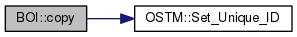
\includegraphics[width=302pt]{class_b_o_i_a9ff2d32c25c23a1bea6316f50c3bf677_cgraph}
\end{center}
\end{figure}




Here is the caller graph for this function\+:\nopagebreak
\begin{figure}[H]
\begin{center}
\leavevmode
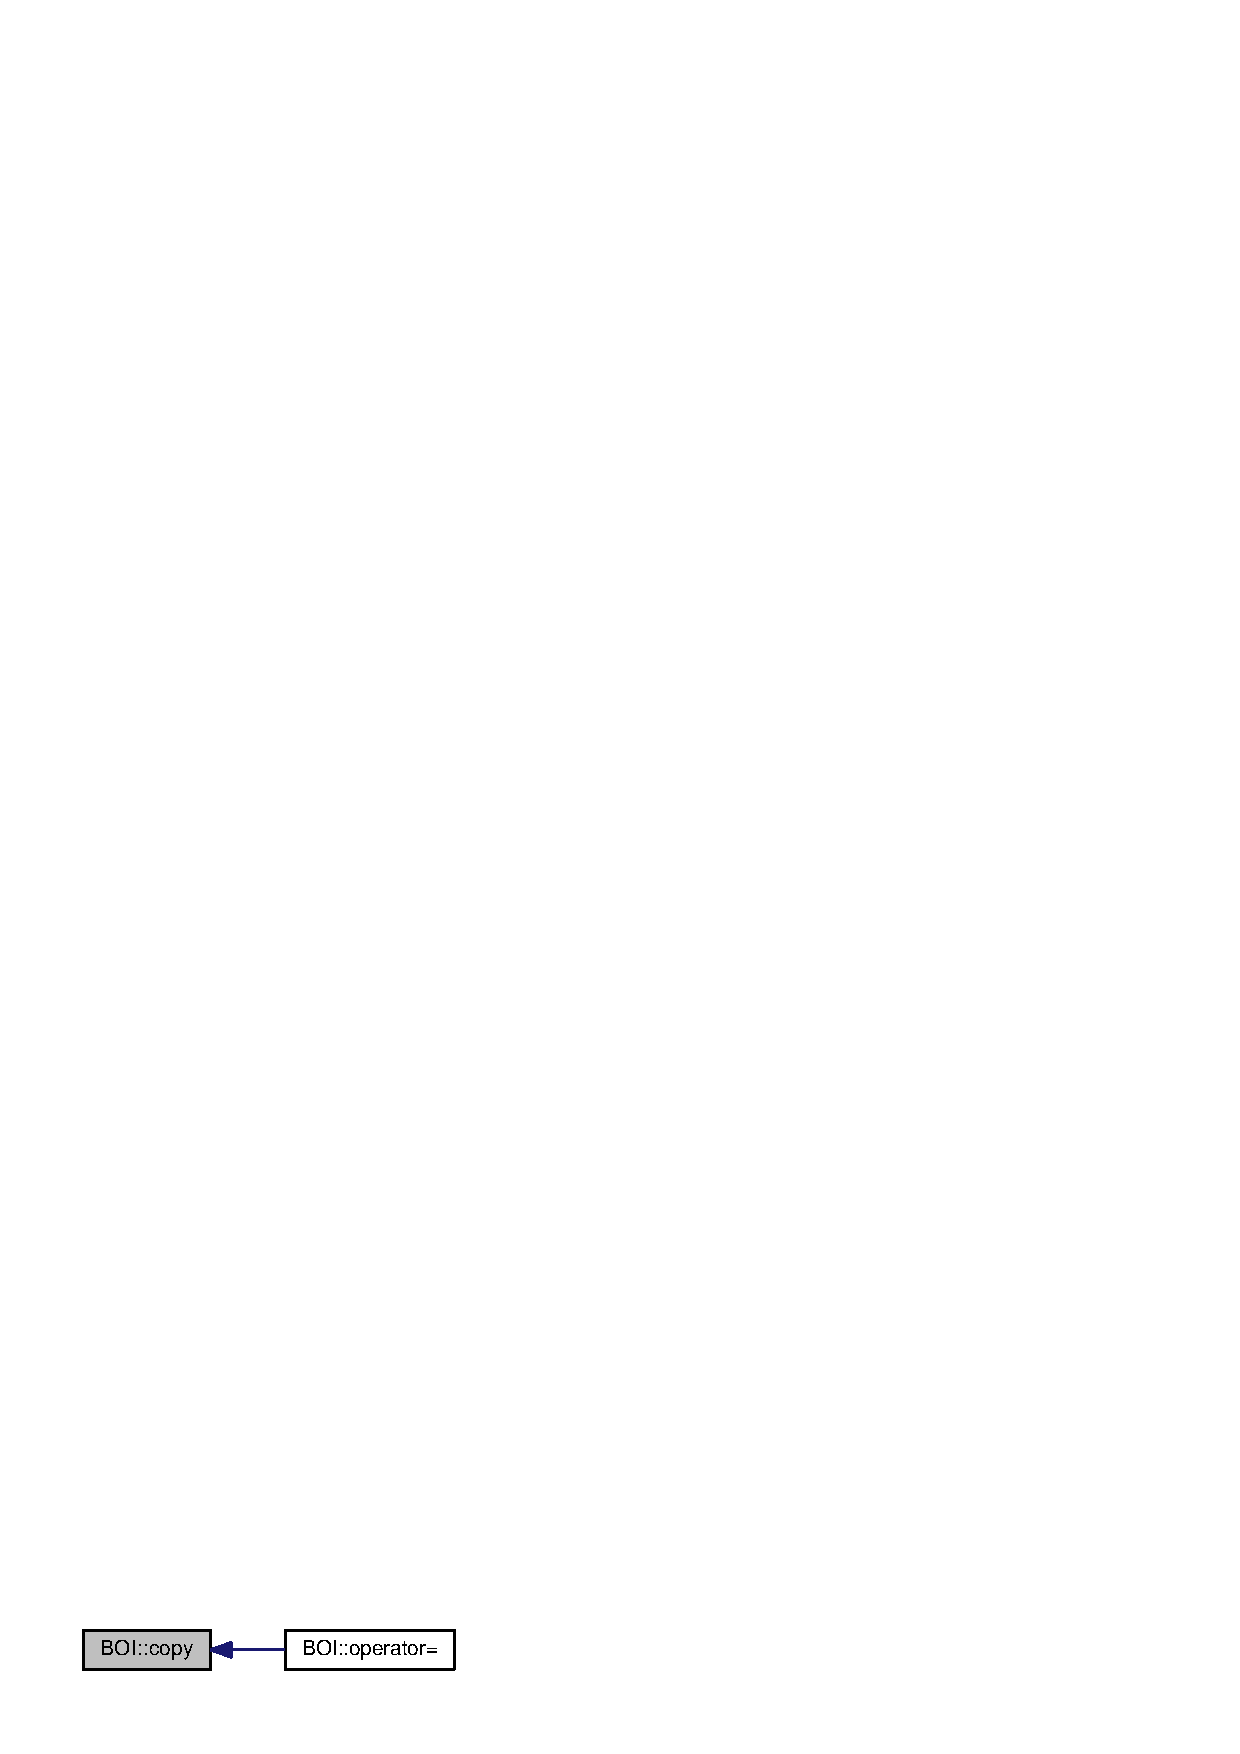
\includegraphics[width=258pt]{class_b_o_i_a9ff2d32c25c23a1bea6316f50c3bf677_icgraph}
\end{center}
\end{figure}


\index{B\+OI@{B\+OI}!Get\+Account\+Number@{Get\+Account\+Number}}
\index{Get\+Account\+Number@{Get\+Account\+Number}!B\+OI@{B\+OI}}
\paragraph[{\texorpdfstring{Get\+Account\+Number() const }{GetAccountNumber() const }}]{\setlength{\rightskip}{0pt plus 5cm}int B\+O\+I\+::\+Get\+Account\+Number (
\begin{DoxyParamCaption}
{}
\end{DoxyParamCaption}
) const\hspace{0.3cm}{\ttfamily [virtual]}}\hypertarget{class_b_o_i_a5b18e1538f3d37835234946cdf9f240f}{}\label{class_b_o_i_a5b18e1538f3d37835234946cdf9f240f}


Implements \hyperlink{class_b_a_n_k_a781f774d1b3fd7437563811b015cbc8c}{B\+A\+NK}.



Definition at line \hyperlink{_b_o_i_8cpp_source_l00078}{78} of file \hyperlink{_b_o_i_8cpp_source}{B\+O\+I.\+cpp}.



Referenced by \hyperlink{_b_o_i_8h_source_l00065}{operator=()}, and \hyperlink{_b_o_i_8cpp_source_l00054}{to\+String()}.


\begin{DoxyCode}
00078                                 \{
00079     \textcolor{keywordflow}{return} accountNumber;
00080 \}
\end{DoxyCode}


Here is the caller graph for this function\+:\nopagebreak
\begin{figure}[H]
\begin{center}
\leavevmode
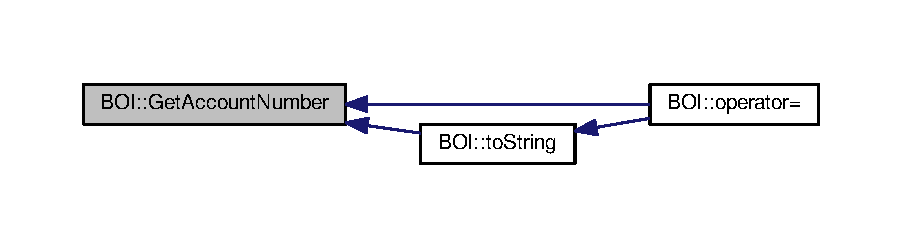
\includegraphics[width=350pt]{class_b_o_i_a5b18e1538f3d37835234946cdf9f240f_icgraph}
\end{center}
\end{figure}


\index{B\+OI@{B\+OI}!Get\+Address@{Get\+Address}}
\index{Get\+Address@{Get\+Address}!B\+OI@{B\+OI}}
\paragraph[{\texorpdfstring{Get\+Address() const }{GetAddress() const }}]{\setlength{\rightskip}{0pt plus 5cm}std\+::string B\+O\+I\+::\+Get\+Address (
\begin{DoxyParamCaption}
{}
\end{DoxyParamCaption}
) const\hspace{0.3cm}{\ttfamily [virtual]}}\hypertarget{class_b_o_i_a8920e1f47b22445ba954e86012207462}{}\label{class_b_o_i_a8920e1f47b22445ba954e86012207462}


Implements \hyperlink{class_b_a_n_k_af1847278d240ceb2b831f03c7e039e07}{B\+A\+NK}.



Definition at line \hyperlink{_b_o_i_8cpp_source_l00062}{62} of file \hyperlink{_b_o_i_8cpp_source}{B\+O\+I.\+cpp}.



Referenced by \hyperlink{_b_o_i_8h_source_l00065}{operator=()}.


\begin{DoxyCode}
00062                                 \{
00063     \textcolor{keywordflow}{return} address;
00064 \}
\end{DoxyCode}


Here is the caller graph for this function\+:\nopagebreak
\begin{figure}[H]
\begin{center}
\leavevmode
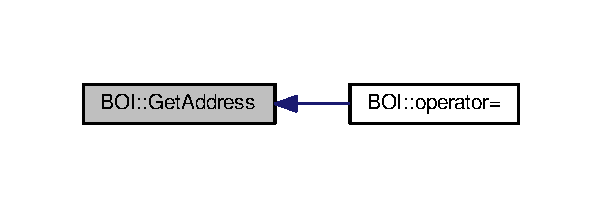
\includegraphics[width=289pt]{class_b_o_i_a8920e1f47b22445ba954e86012207462_icgraph}
\end{center}
\end{figure}


\index{B\+OI@{B\+OI}!Get\+Balance@{Get\+Balance}}
\index{Get\+Balance@{Get\+Balance}!B\+OI@{B\+OI}}
\paragraph[{\texorpdfstring{Get\+Balance() const }{GetBalance() const }}]{\setlength{\rightskip}{0pt plus 5cm}double B\+O\+I\+::\+Get\+Balance (
\begin{DoxyParamCaption}
{}
\end{DoxyParamCaption}
) const\hspace{0.3cm}{\ttfamily [virtual]}}\hypertarget{class_b_o_i_a25b289dece2a1685bb9d1a9332c9be0b}{}\label{class_b_o_i_a25b289dece2a1685bb9d1a9332c9be0b}


Implements \hyperlink{class_b_a_n_k_ae0fc62108895cddad418b23cb6d15f58}{B\+A\+NK}.



Definition at line \hyperlink{_b_o_i_8cpp_source_l00070}{70} of file \hyperlink{_b_o_i_8cpp_source}{B\+O\+I.\+cpp}.



Referenced by \hyperlink{_b_o_i_8h_source_l00065}{operator=()}, and \hyperlink{_b_o_i_8cpp_source_l00054}{to\+String()}.


\begin{DoxyCode}
00070                              \{
00071     \textcolor{keywordflow}{return} balance;
00072 \}
\end{DoxyCode}


Here is the caller graph for this function\+:\nopagebreak
\begin{figure}[H]
\begin{center}
\leavevmode
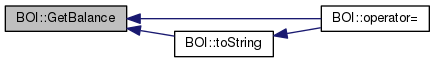
\includegraphics[width=350pt]{class_b_o_i_a25b289dece2a1685bb9d1a9332c9be0b_icgraph}
\end{center}
\end{figure}


\index{B\+OI@{B\+OI}!get\+Base\+Copy@{get\+Base\+Copy}}
\index{get\+Base\+Copy@{get\+Base\+Copy}!B\+OI@{B\+OI}}
\paragraph[{\texorpdfstring{get\+Base\+Copy(std\+::shared\+\_\+ptr$<$ O\+S\+T\+M $>$ object)}{getBaseCopy(std::shared_ptr< OSTM > object)}}]{\setlength{\rightskip}{0pt plus 5cm}std\+::shared\+\_\+ptr$<$ O\+S\+TM $>$ B\+O\+I\+::get\+Base\+Copy (
\begin{DoxyParamCaption}
\item[{std\+::shared\+\_\+ptr$<$ O\+S\+TM $>$}]{object}
\end{DoxyParamCaption}
)\hspace{0.3cm}{\ttfamily [virtual]}}\hypertarget{class_b_o_i_ad53ae2918a656793b9d7a670d35ecfa3}{}\label{class_b_o_i_ad53ae2918a656793b9d7a670d35ecfa3}


get\+Base\+Copy function, make deep copy of the object/pointer and Return a new B\+A\+N\+K$\ast$ type object 


\begin{DoxyParams}{Parameters}
{\em obj\+TO} & is a \hyperlink{class_b_a_n_k}{B\+A\+NK} type pointer for casting \\
\hline
{\em obj} & is a B\+A\+N\+K$\ast$ return type \\
\hline
\end{DoxyParams}


Definition at line \hyperlink{_b_o_i_8cpp_source_l00022}{22} of file \hyperlink{_b_o_i_8cpp_source}{B\+O\+I.\+cpp}.



References \hyperlink{_b_o_i_8h_source_l00024}{B\+O\+I()}.



Referenced by \hyperlink{_b_o_i_8h_source_l00065}{operator=()}.


\begin{DoxyCode}
00023 \{
00024 
00025     std::shared\_ptr<BOI> objTO = std::dynamic\_pointer\_cast<\hyperlink{class_b_o_i}{BOI}>(object);
00026     std::shared\_ptr<BOI> obj(\textcolor{keyword}{new} \hyperlink{class_b_o_i_a6af682a5f199a029681f0cb2b8658706}{BOI}(objTO,object->Get\_Version(),\textcolor{keywordtype}{object}->Get\_Unique\_ID())); 
00027     std::shared\_ptr<OSTM> ostm\_obj = std::dynamic\_pointer\_cast<OSTM>(obj);
00028     \textcolor{keywordflow}{return} ostm\_obj;
00029 \}
\end{DoxyCode}


Here is the call graph for this function\+:\nopagebreak
\begin{figure}[H]
\begin{center}
\leavevmode
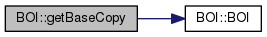
\includegraphics[width=272pt]{class_b_o_i_ad53ae2918a656793b9d7a670d35ecfa3_cgraph}
\end{center}
\end{figure}




Here is the caller graph for this function\+:\nopagebreak
\begin{figure}[H]
\begin{center}
\leavevmode
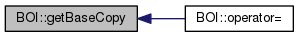
\includegraphics[width=296pt]{class_b_o_i_ad53ae2918a656793b9d7a670d35ecfa3_icgraph}
\end{center}
\end{figure}


\index{B\+OI@{B\+OI}!Get\+First\+Name@{Get\+First\+Name}}
\index{Get\+First\+Name@{Get\+First\+Name}!B\+OI@{B\+OI}}
\paragraph[{\texorpdfstring{Get\+First\+Name() const }{GetFirstName() const }}]{\setlength{\rightskip}{0pt plus 5cm}std\+::string B\+O\+I\+::\+Get\+First\+Name (
\begin{DoxyParamCaption}
{}
\end{DoxyParamCaption}
) const\hspace{0.3cm}{\ttfamily [virtual]}}\hypertarget{class_b_o_i_ab4b9d50c6008a666aa4382def580e7d1}{}\label{class_b_o_i_ab4b9d50c6008a666aa4382def580e7d1}


Implements \hyperlink{class_b_a_n_k_a6b50fbebbe0d807ff3bc36ad6dbe01b8}{B\+A\+NK}.



Definition at line \hyperlink{_b_o_i_8cpp_source_l00094}{94} of file \hyperlink{_b_o_i_8cpp_source}{B\+O\+I.\+cpp}.



Referenced by \hyperlink{_b_o_i_8h_source_l00065}{operator=()}, and \hyperlink{_b_o_i_8cpp_source_l00054}{to\+String()}.


\begin{DoxyCode}
00094                                   \{
00095     \textcolor{keywordflow}{return} firstName;
00096 \}
\end{DoxyCode}


Here is the caller graph for this function\+:\nopagebreak
\begin{figure}[H]
\begin{center}
\leavevmode
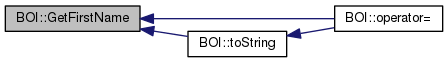
\includegraphics[width=350pt]{class_b_o_i_ab4b9d50c6008a666aa4382def580e7d1_icgraph}
\end{center}
\end{figure}


\index{B\+OI@{B\+OI}!Get\+Fullname@{Get\+Fullname}}
\index{Get\+Fullname@{Get\+Fullname}!B\+OI@{B\+OI}}
\paragraph[{\texorpdfstring{Get\+Fullname() const }{GetFullname() const }}]{\setlength{\rightskip}{0pt plus 5cm}std\+::string B\+O\+I\+::\+Get\+Fullname (
\begin{DoxyParamCaption}
{}
\end{DoxyParamCaption}
) const\hspace{0.3cm}{\ttfamily [virtual]}}\hypertarget{class_b_o_i_af56446a377068cd65526e40e8b31b878}{}\label{class_b_o_i_af56446a377068cd65526e40e8b31b878}


Implements \hyperlink{class_b_a_n_k_a05d6f0670c42e995ebd72cd4ade4305f}{B\+A\+NK}.



Definition at line \hyperlink{_b_o_i_8cpp_source_l00102}{102} of file \hyperlink{_b_o_i_8cpp_source}{B\+O\+I.\+cpp}.



Referenced by \hyperlink{_b_o_i_8h_source_l00065}{operator=()}.


\begin{DoxyCode}
00102                                  \{
00103     \textcolor{keywordflow}{return} fullname;
00104 \}
\end{DoxyCode}


Here is the caller graph for this function\+:\nopagebreak
\begin{figure}[H]
\begin{center}
\leavevmode
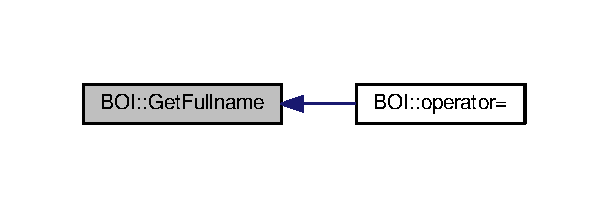
\includegraphics[width=292pt]{class_b_o_i_af56446a377068cd65526e40e8b31b878_icgraph}
\end{center}
\end{figure}


\index{B\+OI@{B\+OI}!Get\+Last\+Name@{Get\+Last\+Name}}
\index{Get\+Last\+Name@{Get\+Last\+Name}!B\+OI@{B\+OI}}
\paragraph[{\texorpdfstring{Get\+Last\+Name() const }{GetLastName() const }}]{\setlength{\rightskip}{0pt plus 5cm}std\+::string B\+O\+I\+::\+Get\+Last\+Name (
\begin{DoxyParamCaption}
{}
\end{DoxyParamCaption}
) const\hspace{0.3cm}{\ttfamily [virtual]}}\hypertarget{class_b_o_i_a37828f3fa4a32f522966e2cad90eaab2}{}\label{class_b_o_i_a37828f3fa4a32f522966e2cad90eaab2}


Implements \hyperlink{class_b_a_n_k_a6588652e6baae302caa39228ecf1606a}{B\+A\+NK}.



Definition at line \hyperlink{_b_o_i_8cpp_source_l00086}{86} of file \hyperlink{_b_o_i_8cpp_source}{B\+O\+I.\+cpp}.



Referenced by \hyperlink{_b_o_i_8h_source_l00065}{operator=()}, and \hyperlink{_b_o_i_8cpp_source_l00054}{to\+String()}.


\begin{DoxyCode}
00086                                  \{
00087     \textcolor{keywordflow}{return} lastName;
00088 \}
\end{DoxyCode}


Here is the caller graph for this function\+:\nopagebreak
\begin{figure}[H]
\begin{center}
\leavevmode
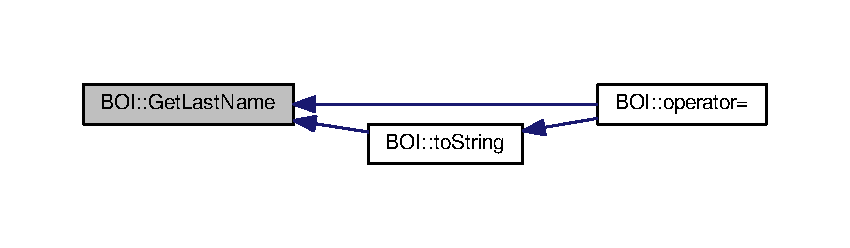
\includegraphics[width=350pt]{class_b_o_i_a37828f3fa4a32f522966e2cad90eaab2_icgraph}
\end{center}
\end{figure}


\index{B\+OI@{B\+OI}!operator=@{operator=}}
\index{operator=@{operator=}!B\+OI@{B\+OI}}
\paragraph[{\texorpdfstring{operator=(const B\+O\+I \&orig)}{operator=(const BOI &orig)}}]{\setlength{\rightskip}{0pt plus 5cm}{\bf B\+OI} B\+O\+I\+::operator= (
\begin{DoxyParamCaption}
\item[{const {\bf B\+OI} \&}]{orig}
\end{DoxyParamCaption}
)\hspace{0.3cm}{\ttfamily [inline]}}\hypertarget{class_b_o_i_a4b4a3976cc13c4d3de0d7ff8882a7af3}{}\label{class_b_o_i_a4b4a3976cc13c4d3de0d7ff8882a7af3}
Operator 

Definition at line \hyperlink{_b_o_i_8h_source_l00065}{65} of file \hyperlink{_b_o_i_8h_source}{B\+O\+I.\+h}.



References \hyperlink{_b_o_i_8cpp_source_l00035}{copy()}, \hyperlink{_b_o_i_8cpp_source_l00078}{Get\+Account\+Number()}, \hyperlink{_b_o_i_8cpp_source_l00062}{Get\+Address()}, \hyperlink{_b_o_i_8cpp_source_l00070}{Get\+Balance()}, \hyperlink{_b_o_i_8cpp_source_l00022}{get\+Base\+Copy()}, \hyperlink{_b_o_i_8cpp_source_l00094}{Get\+First\+Name()}, \hyperlink{_b_o_i_8cpp_source_l00102}{Get\+Fullname()}, \hyperlink{_b_o_i_8cpp_source_l00086}{Get\+Last\+Name()}, \hyperlink{_b_o_i_8cpp_source_l00074}{Set\+Account\+Number()}, \hyperlink{_b_o_i_8cpp_source_l00058}{Set\+Address()}, \hyperlink{_b_o_i_8cpp_source_l00066}{Set\+Balance()}, \hyperlink{_b_o_i_8cpp_source_l00090}{Set\+First\+Name()}, \hyperlink{_b_o_i_8cpp_source_l00098}{Set\+Fullname()}, \hyperlink{_b_o_i_8cpp_source_l00082}{Set\+Last\+Name()}, \hyperlink{_b_o_i_8cpp_source_l00054}{to\+String()}, and \hyperlink{_b_o_i_8cpp_source_l00012}{$\sim$\+B\+O\+I()}.


\begin{DoxyCode}
00065 \{\};
\end{DoxyCode}


Here is the call graph for this function\+:\nopagebreak
\begin{figure}[H]
\begin{center}
\leavevmode
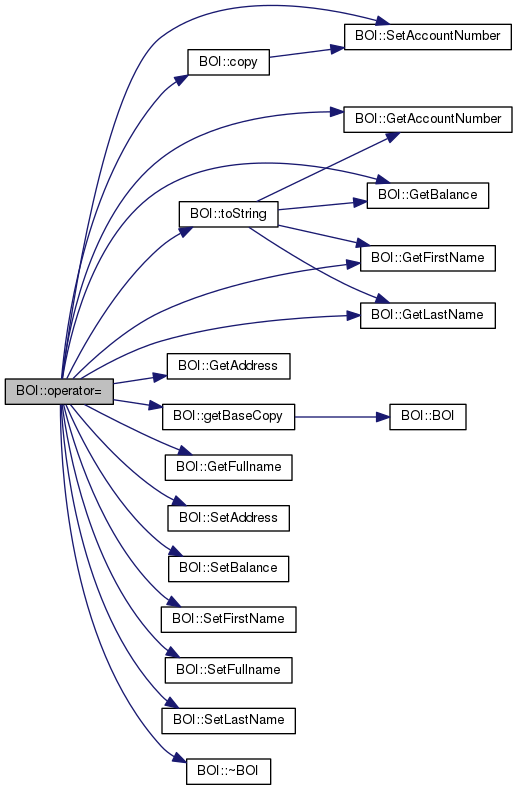
\includegraphics[width=350pt]{class_b_o_i_a4b4a3976cc13c4d3de0d7ff8882a7af3_cgraph}
\end{center}
\end{figure}


\index{B\+OI@{B\+OI}!Set\+Account\+Number@{Set\+Account\+Number}}
\index{Set\+Account\+Number@{Set\+Account\+Number}!B\+OI@{B\+OI}}
\paragraph[{\texorpdfstring{Set\+Account\+Number(int account\+Number)}{SetAccountNumber(int accountNumber)}}]{\setlength{\rightskip}{0pt plus 5cm}void B\+O\+I\+::\+Set\+Account\+Number (
\begin{DoxyParamCaption}
\item[{int}]{account\+Number}
\end{DoxyParamCaption}
)\hspace{0.3cm}{\ttfamily [virtual]}}\hypertarget{class_b_o_i_affc9e7e2a36214b3790f250b7108bb65}{}\label{class_b_o_i_affc9e7e2a36214b3790f250b7108bb65}


Implements \hyperlink{class_b_a_n_k_a1134e7e3d219b7a3aaee42410aa19dfb}{B\+A\+NK}.



Definition at line \hyperlink{_b_o_i_8cpp_source_l00074}{74} of file \hyperlink{_b_o_i_8cpp_source}{B\+O\+I.\+cpp}.



Referenced by \hyperlink{_b_o_i_8cpp_source_l00035}{copy()}, and \hyperlink{_b_o_i_8h_source_l00065}{operator=()}.


\begin{DoxyCode}
00074                                             \{
00075     this->accountNumber = accountNumber;
00076 \}
\end{DoxyCode}


Here is the caller graph for this function\+:\nopagebreak
\begin{figure}[H]
\begin{center}
\leavevmode
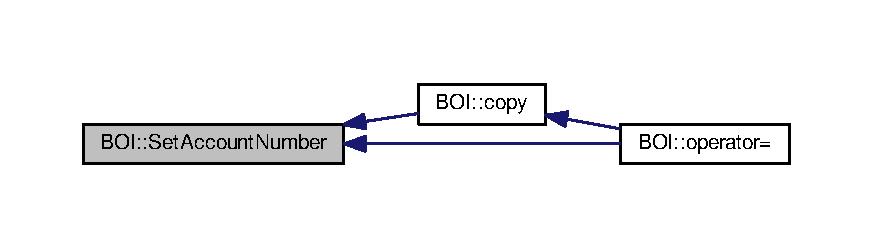
\includegraphics[width=350pt]{class_b_o_i_affc9e7e2a36214b3790f250b7108bb65_icgraph}
\end{center}
\end{figure}


\index{B\+OI@{B\+OI}!Set\+Address@{Set\+Address}}
\index{Set\+Address@{Set\+Address}!B\+OI@{B\+OI}}
\paragraph[{\texorpdfstring{Set\+Address(std\+::string address)}{SetAddress(std::string address)}}]{\setlength{\rightskip}{0pt plus 5cm}void B\+O\+I\+::\+Set\+Address (
\begin{DoxyParamCaption}
\item[{std\+::string}]{address}
\end{DoxyParamCaption}
)\hspace{0.3cm}{\ttfamily [virtual]}}\hypertarget{class_b_o_i_a00c9386c862cf2442968bf7fc30102b3}{}\label{class_b_o_i_a00c9386c862cf2442968bf7fc30102b3}


Implements \hyperlink{class_b_a_n_k_a4044c2f37c8b55b65ed5d57f1867e508}{B\+A\+NK}.



Definition at line \hyperlink{_b_o_i_8cpp_source_l00058}{58} of file \hyperlink{_b_o_i_8cpp_source}{B\+O\+I.\+cpp}.



Referenced by \hyperlink{_b_o_i_8h_source_l00065}{operator=()}.


\begin{DoxyCode}
00058                                       \{
00059     this->address = address;
00060 \}
\end{DoxyCode}


Here is the caller graph for this function\+:\nopagebreak
\begin{figure}[H]
\begin{center}
\leavevmode
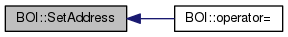
\includegraphics[width=288pt]{class_b_o_i_a00c9386c862cf2442968bf7fc30102b3_icgraph}
\end{center}
\end{figure}


\index{B\+OI@{B\+OI}!Set\+Balance@{Set\+Balance}}
\index{Set\+Balance@{Set\+Balance}!B\+OI@{B\+OI}}
\paragraph[{\texorpdfstring{Set\+Balance(double balance)}{SetBalance(double balance)}}]{\setlength{\rightskip}{0pt plus 5cm}void B\+O\+I\+::\+Set\+Balance (
\begin{DoxyParamCaption}
\item[{double}]{balance}
\end{DoxyParamCaption}
)\hspace{0.3cm}{\ttfamily [virtual]}}\hypertarget{class_b_o_i_a416667693c10f5e4120eec97a9269348}{}\label{class_b_o_i_a416667693c10f5e4120eec97a9269348}


Implements \hyperlink{class_b_a_n_k_a43bef9f486c88a2dc4906eee0e38a394}{B\+A\+NK}.



Definition at line \hyperlink{_b_o_i_8cpp_source_l00066}{66} of file \hyperlink{_b_o_i_8cpp_source}{B\+O\+I.\+cpp}.



Referenced by \hyperlink{_b_o_i_8h_source_l00065}{operator=()}.


\begin{DoxyCode}
00066                                    \{
00067     this->balance = balance;
00068 \}
\end{DoxyCode}


Here is the caller graph for this function\+:\nopagebreak
\begin{figure}[H]
\begin{center}
\leavevmode
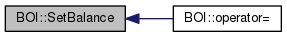
\includegraphics[width=287pt]{class_b_o_i_a416667693c10f5e4120eec97a9269348_icgraph}
\end{center}
\end{figure}


\index{B\+OI@{B\+OI}!Set\+First\+Name@{Set\+First\+Name}}
\index{Set\+First\+Name@{Set\+First\+Name}!B\+OI@{B\+OI}}
\paragraph[{\texorpdfstring{Set\+First\+Name(std\+::string first\+Name)}{SetFirstName(std::string firstName)}}]{\setlength{\rightskip}{0pt plus 5cm}void B\+O\+I\+::\+Set\+First\+Name (
\begin{DoxyParamCaption}
\item[{std\+::string}]{first\+Name}
\end{DoxyParamCaption}
)\hspace{0.3cm}{\ttfamily [virtual]}}\hypertarget{class_b_o_i_ae9042f87be085c2cec799981c30d7d19}{}\label{class_b_o_i_ae9042f87be085c2cec799981c30d7d19}


Implements \hyperlink{class_b_a_n_k_a4baa20e9389c4a592cb0d172c053bf4e}{B\+A\+NK}.



Definition at line \hyperlink{_b_o_i_8cpp_source_l00090}{90} of file \hyperlink{_b_o_i_8cpp_source}{B\+O\+I.\+cpp}.



Referenced by \hyperlink{_b_o_i_8h_source_l00065}{operator=()}.


\begin{DoxyCode}
00090                                           \{
00091     this->firstName = firstName;
00092 \}
\end{DoxyCode}


Here is the caller graph for this function\+:\nopagebreak
\begin{figure}[H]
\begin{center}
\leavevmode
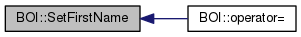
\includegraphics[width=298pt]{class_b_o_i_ae9042f87be085c2cec799981c30d7d19_icgraph}
\end{center}
\end{figure}


\index{B\+OI@{B\+OI}!Set\+Fullname@{Set\+Fullname}}
\index{Set\+Fullname@{Set\+Fullname}!B\+OI@{B\+OI}}
\paragraph[{\texorpdfstring{Set\+Fullname(std\+::string fullname)}{SetFullname(std::string fullname)}}]{\setlength{\rightskip}{0pt plus 5cm}void B\+O\+I\+::\+Set\+Fullname (
\begin{DoxyParamCaption}
\item[{std\+::string}]{fullname}
\end{DoxyParamCaption}
)\hspace{0.3cm}{\ttfamily [virtual]}}\hypertarget{class_b_o_i_a93091f16610f1a1474aea31fd5f81ffd}{}\label{class_b_o_i_a93091f16610f1a1474aea31fd5f81ffd}


Implements \hyperlink{class_b_a_n_k_a02a2f543667403bad41ad614ac9bbde2}{B\+A\+NK}.



Definition at line \hyperlink{_b_o_i_8cpp_source_l00098}{98} of file \hyperlink{_b_o_i_8cpp_source}{B\+O\+I.\+cpp}.



Referenced by \hyperlink{_b_o_i_8h_source_l00065}{operator=()}.


\begin{DoxyCode}
00098                                         \{
00099     this->fullname = fullname;
00100 \}
\end{DoxyCode}


Here is the caller graph for this function\+:\nopagebreak
\begin{figure}[H]
\begin{center}
\leavevmode
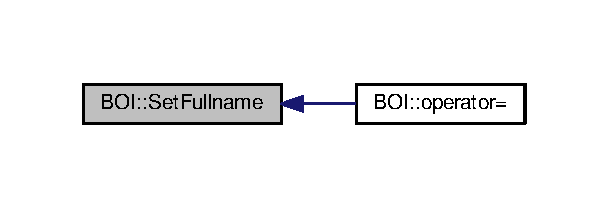
\includegraphics[width=292pt]{class_b_o_i_a93091f16610f1a1474aea31fd5f81ffd_icgraph}
\end{center}
\end{figure}


\index{B\+OI@{B\+OI}!Set\+Last\+Name@{Set\+Last\+Name}}
\index{Set\+Last\+Name@{Set\+Last\+Name}!B\+OI@{B\+OI}}
\paragraph[{\texorpdfstring{Set\+Last\+Name(std\+::string last\+Name)}{SetLastName(std::string lastName)}}]{\setlength{\rightskip}{0pt plus 5cm}void B\+O\+I\+::\+Set\+Last\+Name (
\begin{DoxyParamCaption}
\item[{std\+::string}]{last\+Name}
\end{DoxyParamCaption}
)\hspace{0.3cm}{\ttfamily [virtual]}}\hypertarget{class_b_o_i_a663906e9a59ffa970fb928746c01e8af}{}\label{class_b_o_i_a663906e9a59ffa970fb928746c01e8af}


Implements \hyperlink{class_b_a_n_k_a480fa0973e3e27df92be6767b2f9a652}{B\+A\+NK}.



Definition at line \hyperlink{_b_o_i_8cpp_source_l00082}{82} of file \hyperlink{_b_o_i_8cpp_source}{B\+O\+I.\+cpp}.



Referenced by \hyperlink{_b_o_i_8h_source_l00065}{operator=()}.


\begin{DoxyCode}
00082                                         \{
00083     this->lastName = lastName;
00084 \}
\end{DoxyCode}


Here is the caller graph for this function\+:\nopagebreak
\begin{figure}[H]
\begin{center}
\leavevmode
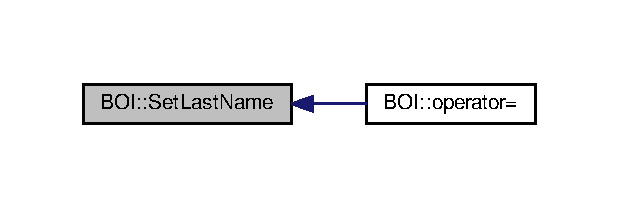
\includegraphics[width=297pt]{class_b_o_i_a663906e9a59ffa970fb928746c01e8af_icgraph}
\end{center}
\end{figure}


\index{B\+OI@{B\+OI}!to\+String@{to\+String}}
\index{to\+String@{to\+String}!B\+OI@{B\+OI}}
\paragraph[{\texorpdfstring{to\+String()}{toString()}}]{\setlength{\rightskip}{0pt plus 5cm}void B\+O\+I\+::to\+String (
\begin{DoxyParamCaption}
{}
\end{DoxyParamCaption}
)\hspace{0.3cm}{\ttfamily [virtual]}}\hypertarget{class_b_o_i_ab02a4dd4ebcc5b2abfaca19f2dff2006}{}\label{class_b_o_i_ab02a4dd4ebcc5b2abfaca19f2dff2006}


\+\_\+cast, is use to cast bak the std\+::shared\+\_\+ptr$<$\+O\+S\+T\+M$>$ to the required type 

to\+String function, displays the object values in formatted way 

Definition at line \hyperlink{_b_o_i_8cpp_source_l00054}{54} of file \hyperlink{_b_o_i_8cpp_source}{B\+O\+I.\+cpp}.



References \hyperlink{_b_o_i_8cpp_source_l00078}{Get\+Account\+Number()}, \hyperlink{_b_o_i_8cpp_source_l00070}{Get\+Balance()}, \hyperlink{_b_o_i_8cpp_source_l00094}{Get\+First\+Name()}, and \hyperlink{_b_o_i_8cpp_source_l00086}{Get\+Last\+Name()}.



Referenced by \hyperlink{_b_o_i_8h_source_l00065}{operator=()}.


\begin{DoxyCode}
00055 \{
00056    std::cout << \textcolor{stringliteral}{"\(\backslash\)nBOI BANK"} << \textcolor{stringliteral}{"\(\backslash\)nUnique ID : "} << this->Get\_Unique\_ID() << \textcolor{stringliteral}{"\(\backslash\)nInt account : "} << this->
      \hyperlink{class_b_o_i_a5b18e1538f3d37835234946cdf9f240f}{GetAccountNumber}() << \textcolor{stringliteral}{"\(\backslash\)nDouble value : "} << this->\hyperlink{class_b_o_i_a25b289dece2a1685bb9d1a9332c9be0b}{GetBalance}() << \textcolor{stringliteral}{"\(\backslash\)nFirst name:
       "} << this->\hyperlink{class_b_o_i_ab4b9d50c6008a666aa4382def580e7d1}{GetFirstName}() << \textcolor{stringliteral}{"\(\backslash\)nLast name : "} << this->\hyperlink{class_b_o_i_a37828f3fa4a32f522966e2cad90eaab2}{GetLastName}()  << \textcolor{stringliteral}{"\(\backslash\)nVersion
       number : "} << this->Get\_Version() << std::endl;
00057 \}
\end{DoxyCode}


Here is the call graph for this function\+:\nopagebreak
\begin{figure}[H]
\begin{center}
\leavevmode
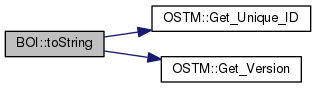
\includegraphics[width=316pt]{class_b_o_i_ab02a4dd4ebcc5b2abfaca19f2dff2006_cgraph}
\end{center}
\end{figure}




Here is the caller graph for this function\+:\nopagebreak
\begin{figure}[H]
\begin{center}
\leavevmode
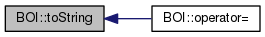
\includegraphics[width=271pt]{class_b_o_i_ab02a4dd4ebcc5b2abfaca19f2dff2006_icgraph}
\end{center}
\end{figure}




The documentation for this class was generated from the following files\+:\begin{DoxyCompactItemize}
\item 
\hyperlink{_b_o_i_8h}{B\+O\+I.\+h}\item 
\hyperlink{_b_o_i_8cpp}{B\+O\+I.\+cpp}\end{DoxyCompactItemize}

\section{C\+A\+R\+L\+O\+W\+\_\+W Class Reference}
\label{class_c_a_r_l_o_w___w}\index{C\+A\+R\+L\+O\+W\+\_\+W@{C\+A\+R\+L\+O\+W\+\_\+W}}


{\ttfamily \#include $<$C\+A\+R\+L\+O\+W\+\_\+\+W.\+h$>$}

Inheritance diagram for C\+A\+R\+L\+O\+W\+\_\+W\+:\begin{figure}[H]
\begin{center}
\leavevmode
\includegraphics[height=3.000000cm]{class_c_a_r_l_o_w___w}
\end{center}
\end{figure}
\subsection*{Public Member Functions}
\begin{DoxyCompactItemize}
\item 
{\bf C\+A\+R\+L\+O\+W\+\_\+W} ()
\item 
{\bf C\+A\+R\+L\+O\+W\+\_\+W} (std\+::string address, std\+::string shop\+\_\+name, int iphone, int samsung, int sony, int huawei, int nokia, int alcatel)
\item 
{\bf C\+A\+R\+L\+O\+W\+\_\+W} (std\+::shared\+\_\+ptr$<$ {\bf W\+A\+R\+E\+H\+O\+U\+SE} $>$ obj, int \+\_\+version, int \+\_\+unique\+\_\+id)
\item 
{\bf C\+A\+R\+L\+O\+W\+\_\+W} (const {\bf C\+A\+R\+L\+O\+W\+\_\+W} \&orig)
\item 
{\bf C\+A\+R\+L\+O\+W\+\_\+W} {\bf operator=} (const {\bf C\+A\+R\+L\+O\+W\+\_\+W} \&orig)
\item 
virtual {\bf $\sim$\+C\+A\+R\+L\+O\+W\+\_\+W} ()
\item 
virtual void {\bf copy} (std\+::shared\+\_\+ptr$<$ {\bf O\+S\+TM} $>$ to, std\+::shared\+\_\+ptr$<$ {\bf O\+S\+TM} $>$ from)
\begin{DoxyCompactList}\small\item\em copy function, make deep copy of the object/pointer \end{DoxyCompactList}\item 
virtual std\+::shared\+\_\+ptr$<$ {\bf O\+S\+TM} $>$ {\bf get\+Base\+Copy} (std\+::shared\+\_\+ptr$<$ {\bf O\+S\+TM} $>$ object)
\begin{DoxyCompactList}\small\item\em get\+Base\+Copy function, make deep copy of the object/pointer and Return a new B\+A\+N\+K$\ast$ type object \end{DoxyCompactList}\item 
virtual void {\bf to\+String} ()
\begin{DoxyCompactList}\small\item\em \+\_\+cast, is use to cast bak the std\+::shared\+\_\+ptr$<$\+O\+S\+T\+M$>$ to the required type \end{DoxyCompactList}\item 
virtual void {\bfseries Set\+Number\+\_\+of\+\_\+alcatel} (int \+\_\+number\+\_\+of\+\_\+alcatel)\label{class_c_a_r_l_o_w___w_ad264954806d7fd6c418650a5c7c7defb}

\item 
virtual int {\bfseries Get\+Number\+\_\+of\+\_\+alcatel} ()\label{class_c_a_r_l_o_w___w_ae7ab8852e5eeff1c2cd397126fbac0e7}

\item 
virtual void {\bfseries Set\+Number\+\_\+of\+\_\+nokia} (int \+\_\+number\+\_\+of\+\_\+nokia)\label{class_c_a_r_l_o_w___w_af0f395409df02a42b3e9448d027d0776}

\item 
virtual int {\bfseries Get\+Number\+\_\+of\+\_\+nokia} ()\label{class_c_a_r_l_o_w___w_a4e3a644ee69bc4bc4ab3feac1493192b}

\item 
virtual void {\bfseries Set\+Number\+\_\+of\+\_\+huawei} (int \+\_\+number\+\_\+of\+\_\+huawei)\label{class_c_a_r_l_o_w___w_a016d1d51b091fc1732c2923a3baa2f58}

\item 
virtual int {\bfseries Get\+Number\+\_\+of\+\_\+huawei} ()\label{class_c_a_r_l_o_w___w_aea38b51a44cda35a01beb7d45fa7a2a4}

\item 
virtual void {\bfseries Set\+Number\+\_\+of\+\_\+sony} (int \+\_\+number\+\_\+of\+\_\+sony)\label{class_c_a_r_l_o_w___w_ab255132fb2ef5678d00c74f90acdf2dd}

\item 
virtual int {\bfseries Get\+Number\+\_\+of\+\_\+sony} ()\label{class_c_a_r_l_o_w___w_a6d31219dac9b4d8842e14b7414ed286e}

\item 
virtual void {\bfseries Set\+Number\+\_\+of\+\_\+samsung} (int \+\_\+number\+\_\+of\+\_\+samsung)\label{class_c_a_r_l_o_w___w_a6e629d8043c4c4266ecafa9f6a3e6447}

\item 
virtual int {\bfseries Get\+Number\+\_\+of\+\_\+samsung} ()\label{class_c_a_r_l_o_w___w_aecc697b6d017d88f2bdbe3cea2bf3496}

\item 
virtual void {\bfseries Set\+Number\+\_\+of\+\_\+iphones} (int \+\_\+number\+\_\+of\+\_\+iphones)\label{class_c_a_r_l_o_w___w_ad58af9d68450f4fc70e0e1ecd4b1b498}

\item 
virtual int {\bfseries Get\+Number\+\_\+of\+\_\+iphones} ()\label{class_c_a_r_l_o_w___w_a50395c707116ea1176743ed98c6b1f76}

\item 
virtual void {\bfseries Set\+Shop\+\_\+name} (std\+::string \+\_\+shop\+\_\+name)\label{class_c_a_r_l_o_w___w_a9d0dcf25c0a9eb8be530c27bd2cf8933}

\item 
virtual std\+::string {\bfseries Get\+Shop\+\_\+name} ()\label{class_c_a_r_l_o_w___w_a68235a63964645c525620053a33de863}

\item 
virtual void {\bfseries Set\+Shop\+\_\+address} (std\+::string \+\_\+shop\+\_\+address)\label{class_c_a_r_l_o_w___w_a6f66cd4c060b2b1ac6640768ad5c56e4}

\item 
virtual std\+::string {\bfseries Get\+Shop\+\_\+address} ()\label{class_c_a_r_l_o_w___w_af48a2f69706be684115758820ce79ddd}

\end{DoxyCompactItemize}


\subsection{Detailed Description}
Inherit from \doxyref{W\+A\+R\+E\+H\+O\+U\+SE}{p.}{class_w_a_r_e_h_o_u_s_e} 

Definition at line 19 of file C\+A\+R\+L\+O\+W\+\_\+\+W.\+h.



\subsection{Constructor \& Destructor Documentation}
\index{C\+A\+R\+L\+O\+W\+\_\+W@{C\+A\+R\+L\+O\+W\+\_\+W}!C\+A\+R\+L\+O\+W\+\_\+W@{C\+A\+R\+L\+O\+W\+\_\+W}}
\index{C\+A\+R\+L\+O\+W\+\_\+W@{C\+A\+R\+L\+O\+W\+\_\+W}!C\+A\+R\+L\+O\+W\+\_\+W@{C\+A\+R\+L\+O\+W\+\_\+W}}
\subsubsection[{C\+A\+R\+L\+O\+W\+\_\+\+W()}]{\setlength{\rightskip}{0pt plus 5cm}C\+A\+R\+L\+O\+W\+\_\+\+W\+::\+C\+A\+R\+L\+O\+W\+\_\+W (
\begin{DoxyParamCaption}
{}
\end{DoxyParamCaption}
)\hspace{0.3cm}{\ttfamily [inline]}}\label{class_c_a_r_l_o_w___w_a8ae6ca6f4db7ea5240322fd27824c55a}
Constructor 

Definition at line 24 of file C\+A\+R\+L\+O\+W\+\_\+\+W.\+h.

\index{C\+A\+R\+L\+O\+W\+\_\+W@{C\+A\+R\+L\+O\+W\+\_\+W}!C\+A\+R\+L\+O\+W\+\_\+W@{C\+A\+R\+L\+O\+W\+\_\+W}}
\index{C\+A\+R\+L\+O\+W\+\_\+W@{C\+A\+R\+L\+O\+W\+\_\+W}!C\+A\+R\+L\+O\+W\+\_\+W@{C\+A\+R\+L\+O\+W\+\_\+W}}
\subsubsection[{C\+A\+R\+L\+O\+W\+\_\+\+W(std\+::string address, std\+::string shop\+\_\+name, int iphone, int samsung, int sony, int huawei, int nokia, int alcatel)}]{\setlength{\rightskip}{0pt plus 5cm}C\+A\+R\+L\+O\+W\+\_\+\+W\+::\+C\+A\+R\+L\+O\+W\+\_\+W (
\begin{DoxyParamCaption}
\item[{std\+::string}]{address, }
\item[{std\+::string}]{shop\+\_\+name, }
\item[{int}]{iphone, }
\item[{int}]{samsung, }
\item[{int}]{sony, }
\item[{int}]{huawei, }
\item[{int}]{nokia, }
\item[{int}]{alcatel}
\end{DoxyParamCaption}
)\hspace{0.3cm}{\ttfamily [inline]}}\label{class_c_a_r_l_o_w___w_aa13cfb47255f935a3b27708b68e52129}
Custom constructor 

Definition at line 38 of file C\+A\+R\+L\+O\+W\+\_\+\+W.\+h.

\index{C\+A\+R\+L\+O\+W\+\_\+W@{C\+A\+R\+L\+O\+W\+\_\+W}!C\+A\+R\+L\+O\+W\+\_\+W@{C\+A\+R\+L\+O\+W\+\_\+W}}
\index{C\+A\+R\+L\+O\+W\+\_\+W@{C\+A\+R\+L\+O\+W\+\_\+W}!C\+A\+R\+L\+O\+W\+\_\+W@{C\+A\+R\+L\+O\+W\+\_\+W}}
\subsubsection[{C\+A\+R\+L\+O\+W\+\_\+\+W(std\+::shared\+\_\+ptr$<$ W\+A\+R\+E\+H\+O\+U\+S\+E $>$ obj, int \+\_\+version, int \+\_\+unique\+\_\+id)}]{\setlength{\rightskip}{0pt plus 5cm}C\+A\+R\+L\+O\+W\+\_\+\+W\+::\+C\+A\+R\+L\+O\+W\+\_\+W (
\begin{DoxyParamCaption}
\item[{std\+::shared\+\_\+ptr$<$ {\bf W\+A\+R\+E\+H\+O\+U\+SE} $>$}]{obj, }
\item[{int}]{\+\_\+version, }
\item[{int}]{\+\_\+unique\+\_\+id}
\end{DoxyParamCaption}
)\hspace{0.3cm}{\ttfamily [inline]}}\label{class_c_a_r_l_o_w___w_ad3b772ca2d09eba4a273cb0c7cece747}
Custom constructor, used by the library for deep copying 

Definition at line 55 of file C\+A\+R\+L\+O\+W\+\_\+\+W.\+h.

\index{C\+A\+R\+L\+O\+W\+\_\+W@{C\+A\+R\+L\+O\+W\+\_\+W}!C\+A\+R\+L\+O\+W\+\_\+W@{C\+A\+R\+L\+O\+W\+\_\+W}}
\index{C\+A\+R\+L\+O\+W\+\_\+W@{C\+A\+R\+L\+O\+W\+\_\+W}!C\+A\+R\+L\+O\+W\+\_\+W@{C\+A\+R\+L\+O\+W\+\_\+W}}
\subsubsection[{C\+A\+R\+L\+O\+W\+\_\+\+W(const C\+A\+R\+L\+O\+W\+\_\+\+W \&orig)}]{\setlength{\rightskip}{0pt plus 5cm}C\+A\+R\+L\+O\+W\+\_\+\+W\+::\+C\+A\+R\+L\+O\+W\+\_\+W (
\begin{DoxyParamCaption}
\item[{const {\bf C\+A\+R\+L\+O\+W\+\_\+W} \&}]{orig}
\end{DoxyParamCaption}
)}\label{class_c_a_r_l_o_w___w_a267a2792c59f475740a68953c8437205}
Copy constructor 

Definition at line 17 of file C\+A\+R\+L\+O\+W\+\_\+\+W.\+cpp.

\index{C\+A\+R\+L\+O\+W\+\_\+W@{C\+A\+R\+L\+O\+W\+\_\+W}!````~C\+A\+R\+L\+O\+W\+\_\+W@{$\sim$\+C\+A\+R\+L\+O\+W\+\_\+W}}
\index{````~C\+A\+R\+L\+O\+W\+\_\+W@{$\sim$\+C\+A\+R\+L\+O\+W\+\_\+W}!C\+A\+R\+L\+O\+W\+\_\+W@{C\+A\+R\+L\+O\+W\+\_\+W}}
\subsubsection[{$\sim$\+C\+A\+R\+L\+O\+W\+\_\+\+W()}]{\setlength{\rightskip}{0pt plus 5cm}C\+A\+R\+L\+O\+W\+\_\+\+W\+::$\sim$\+C\+A\+R\+L\+O\+W\+\_\+W (
\begin{DoxyParamCaption}
{}
\end{DoxyParamCaption}
)\hspace{0.3cm}{\ttfamily [virtual]}}\label{class_c_a_r_l_o_w___w_aa628d46e58dfd0517f24499eca88138b}
de-\/constructor 

Definition at line 14 of file C\+A\+R\+L\+O\+W\+\_\+\+W.\+cpp.



\subsection{Member Function Documentation}
\index{C\+A\+R\+L\+O\+W\+\_\+W@{C\+A\+R\+L\+O\+W\+\_\+W}!copy@{copy}}
\index{copy@{copy}!C\+A\+R\+L\+O\+W\+\_\+W@{C\+A\+R\+L\+O\+W\+\_\+W}}
\subsubsection[{copy(std\+::shared\+\_\+ptr$<$ O\+S\+T\+M $>$ to, std\+::shared\+\_\+ptr$<$ O\+S\+T\+M $>$ from)}]{\setlength{\rightskip}{0pt plus 5cm}void C\+A\+R\+L\+O\+W\+\_\+\+W\+::copy (
\begin{DoxyParamCaption}
\item[{std\+::shared\+\_\+ptr$<$ {\bf O\+S\+TM} $>$}]{to, }
\item[{std\+::shared\+\_\+ptr$<$ {\bf O\+S\+TM} $>$}]{from}
\end{DoxyParamCaption}
)\hspace{0.3cm}{\ttfamily [virtual]}}\label{class_c_a_r_l_o_w___w_ac91cb7cbae77752e334e273b97fb988b}


copy function, make deep copy of the object/pointer 


\begin{DoxyParams}{Parameters}
{\em obj\+TO} & is a B\+A\+N\+K$\ast$ type object casted back from std\+::shared\+\_\+ptr$<$\+O\+S\+T\+M$>$ \\
\hline
{\em obj\+F\+R\+OM} & is a B\+A\+N\+K$\ast$ type object casted back from std\+::shared\+\_\+ptr$<$\+O\+S\+T\+M$>$ \\
\hline
\end{DoxyParams}


Reimplemented from {\bf O\+S\+TM} \doxyref{}{p.}{class_o_s_t_m_a535d90fced5adbb70312c92f3778e08d}.



Definition at line 37 of file C\+A\+R\+L\+O\+W\+\_\+\+W.\+cpp.

\index{C\+A\+R\+L\+O\+W\+\_\+W@{C\+A\+R\+L\+O\+W\+\_\+W}!get\+Base\+Copy@{get\+Base\+Copy}}
\index{get\+Base\+Copy@{get\+Base\+Copy}!C\+A\+R\+L\+O\+W\+\_\+W@{C\+A\+R\+L\+O\+W\+\_\+W}}
\subsubsection[{get\+Base\+Copy(std\+::shared\+\_\+ptr$<$ O\+S\+T\+M $>$ object)}]{\setlength{\rightskip}{0pt plus 5cm}std\+::shared\+\_\+ptr$<$ {\bf O\+S\+TM} $>$ C\+A\+R\+L\+O\+W\+\_\+\+W\+::get\+Base\+Copy (
\begin{DoxyParamCaption}
\item[{std\+::shared\+\_\+ptr$<$ {\bf O\+S\+TM} $>$}]{object}
\end{DoxyParamCaption}
)\hspace{0.3cm}{\ttfamily [virtual]}}\label{class_c_a_r_l_o_w___w_a1a76566c3a7c01cf469007741dac6b97}


get\+Base\+Copy function, make deep copy of the object/pointer and Return a new B\+A\+N\+K$\ast$ type object 


\begin{DoxyParams}{Parameters}
{\em obj\+TO} & is a \doxyref{B\+A\+NK}{p.}{class_b_a_n_k} type pointer for casting \\
\hline
{\em obj} & is a B\+A\+N\+K$\ast$ return type \\
\hline
\end{DoxyParams}


Reimplemented from {\bf O\+S\+TM} \doxyref{}{p.}{class_o_s_t_m_a0bfa3763bd441407dd6365f42714f94c}.



Definition at line 24 of file C\+A\+R\+L\+O\+W\+\_\+\+W.\+cpp.

\index{C\+A\+R\+L\+O\+W\+\_\+W@{C\+A\+R\+L\+O\+W\+\_\+W}!operator=@{operator=}}
\index{operator=@{operator=}!C\+A\+R\+L\+O\+W\+\_\+W@{C\+A\+R\+L\+O\+W\+\_\+W}}
\subsubsection[{operator=(const C\+A\+R\+L\+O\+W\+\_\+\+W \&orig)}]{\setlength{\rightskip}{0pt plus 5cm}{\bf C\+A\+R\+L\+O\+W\+\_\+W} C\+A\+R\+L\+O\+W\+\_\+\+W\+::operator= (
\begin{DoxyParamCaption}
\item[{const {\bf C\+A\+R\+L\+O\+W\+\_\+W} \&}]{orig}
\end{DoxyParamCaption}
)\hspace{0.3cm}{\ttfamily [inline]}}\label{class_c_a_r_l_o_w___w_a38c83795abf1751b3e122c74494f4586}
Operator 

Definition at line 75 of file C\+A\+R\+L\+O\+W\+\_\+\+W.\+h.

\index{C\+A\+R\+L\+O\+W\+\_\+W@{C\+A\+R\+L\+O\+W\+\_\+W}!to\+String@{to\+String}}
\index{to\+String@{to\+String}!C\+A\+R\+L\+O\+W\+\_\+W@{C\+A\+R\+L\+O\+W\+\_\+W}}
\subsubsection[{to\+String()}]{\setlength{\rightskip}{0pt plus 5cm}void C\+A\+R\+L\+O\+W\+\_\+\+W\+::to\+String (
\begin{DoxyParamCaption}
{}
\end{DoxyParamCaption}
)\hspace{0.3cm}{\ttfamily [virtual]}}\label{class_c_a_r_l_o_w___w_a79e683650f861b59752fb027a5f16e5a}


\+\_\+cast, is use to cast bak the std\+::shared\+\_\+ptr$<$\+O\+S\+T\+M$>$ to the required type 

to\+String function, displays the object values in formatted way 

Reimplemented from {\bf O\+S\+TM} \doxyref{}{p.}{class_o_s_t_m_a513396a115f2987fd07c203309ae8a59}.



Definition at line 64 of file C\+A\+R\+L\+O\+W\+\_\+\+W.\+cpp.



The documentation for this class was generated from the following files\+:\begin{DoxyCompactItemize}
\item 
/media/zoltan/\+Data/00\+\_\+2018\+\_\+\+I\+T\+Carlow/00\+\_\+\+Modules/06\+\_\+\+Project/\+Documents/\+Git\+\_\+\+Sync/\+Main Tests for Linux/\+Test01/C\+A\+R\+L\+O\+W\+\_\+\+W.\+h\item 
/media/zoltan/\+Data/00\+\_\+2018\+\_\+\+I\+T\+Carlow/00\+\_\+\+Modules/06\+\_\+\+Project/\+Documents/\+Git\+\_\+\+Sync/\+Main Tests for Linux/\+Test01/C\+A\+R\+L\+O\+W\+\_\+\+W.\+cpp\end{DoxyCompactItemize}

\hypertarget{class_c_a_r_p_h_o_n_e___w_a_r_e_h_o_u_s_e}{}\subsection{C\+A\+R\+P\+H\+O\+N\+E\+\_\+\+W\+A\+R\+E\+H\+O\+U\+SE Class Reference}
\label{class_c_a_r_p_h_o_n_e___w_a_r_e_h_o_u_s_e}\index{C\+A\+R\+P\+H\+O\+N\+E\+\_\+\+W\+A\+R\+E\+H\+O\+U\+SE@{C\+A\+R\+P\+H\+O\+N\+E\+\_\+\+W\+A\+R\+E\+H\+O\+U\+SE}}


{\ttfamily \#include $<$C\+A\+R\+P\+H\+O\+N\+E\+\_\+\+W\+A\+R\+E\+H\+O\+U\+S\+E.\+h$>$}



Inheritance diagram for C\+A\+R\+P\+H\+O\+N\+E\+\_\+\+W\+A\+R\+E\+H\+O\+U\+SE\+:\nopagebreak
\begin{figure}[H]
\begin{center}
\leavevmode
\includegraphics[height=550pt]{class_c_a_r_p_h_o_n_e___w_a_r_e_h_o_u_s_e__inherit__graph}
\end{center}
\end{figure}


Collaboration diagram for C\+A\+R\+P\+H\+O\+N\+E\+\_\+\+W\+A\+R\+E\+H\+O\+U\+SE\+:\nopagebreak
\begin{figure}[H]
\begin{center}
\leavevmode
\includegraphics[height=550pt]{class_c_a_r_p_h_o_n_e___w_a_r_e_h_o_u_s_e__coll__graph}
\end{center}
\end{figure}
\subsubsection*{Public Member Functions}
\begin{DoxyCompactItemize}
\item 
\hyperlink{class_c_a_r_p_h_o_n_e___w_a_r_e_h_o_u_s_e_a0acec1e20e236b4debf1e0d26334a868_a0acec1e20e236b4debf1e0d26334a868}{C\+A\+R\+P\+H\+O\+N\+E\+\_\+\+W\+A\+R\+E\+H\+O\+U\+SE} ()
\item 
\hyperlink{class_c_a_r_p_h_o_n_e___w_a_r_e_h_o_u_s_e_a1e61584abd37ed2189143f0c0d4d2e40_a1e61584abd37ed2189143f0c0d4d2e40}{C\+A\+R\+P\+H\+O\+N\+E\+\_\+\+W\+A\+R\+E\+H\+O\+U\+SE} (std\+::string address, std\+::string shop\+\_\+name, int iphone, int samsung, int sony, int huawei, int nokia, int alcatel)
\item 
\hyperlink{class_c_a_r_p_h_o_n_e___w_a_r_e_h_o_u_s_e_a131eb8df5342de81022b166f40f94d92_a131eb8df5342de81022b166f40f94d92}{C\+A\+R\+P\+H\+O\+N\+E\+\_\+\+W\+A\+R\+E\+H\+O\+U\+SE} (std\+::shared\+\_\+ptr$<$ \hyperlink{class_w_a_r_e_h_o_u_s_e}{W\+A\+R\+E\+H\+O\+U\+SE} $>$ obj, int \+\_\+version, int \+\_\+unique\+\_\+id)
\item 
\hyperlink{class_c_a_r_p_h_o_n_e___w_a_r_e_h_o_u_s_e_a7b2446d35d557bdfaa8dbd769f845abb_a7b2446d35d557bdfaa8dbd769f845abb}{C\+A\+R\+P\+H\+O\+N\+E\+\_\+\+W\+A\+R\+E\+H\+O\+U\+SE} (const \hyperlink{class_c_a_r_p_h_o_n_e___w_a_r_e_h_o_u_s_e}{C\+A\+R\+P\+H\+O\+N\+E\+\_\+\+W\+A\+R\+E\+H\+O\+U\+SE} \&orig)
\item 
virtual void \hyperlink{class_c_a_r_p_h_o_n_e___w_a_r_e_h_o_u_s_e_ab9ecf71cd2728f348a5b61df698e054c_ab9ecf71cd2728f348a5b61df698e054c}{copy} (std\+::shared\+\_\+ptr$<$ \hyperlink{class_o_s_t_m}{O\+S\+TM} $>$ to, std\+::shared\+\_\+ptr$<$ \hyperlink{class_o_s_t_m}{O\+S\+TM} $>$ from)
\begin{DoxyCompactList}\small\item\em copy function, make deep copy of the object/pointer \end{DoxyCompactList}\item 
virtual std\+::shared\+\_\+ptr$<$ \hyperlink{class_o_s_t_m}{O\+S\+TM} $>$ \hyperlink{class_c_a_r_p_h_o_n_e___w_a_r_e_h_o_u_s_e_a1d3b2f023c0d6e715416f1e87e7245bb_a1d3b2f023c0d6e715416f1e87e7245bb}{get\+Base\+Copy} (std\+::shared\+\_\+ptr$<$ \hyperlink{class_o_s_t_m}{O\+S\+TM} $>$ object)
\begin{DoxyCompactList}\small\item\em get\+Base\+Copy function, make deep copy of the object/pointer and Return a new B\+A\+N\+K$\ast$ type object \end{DoxyCompactList}\item 
virtual int \hyperlink{class_c_a_r_p_h_o_n_e___w_a_r_e_h_o_u_s_e_a8d278005b2ba46869f6787681ad05704_a8d278005b2ba46869f6787681ad05704}{Get\+Number\+\_\+of\+\_\+alcatel} ()
\item 
virtual int \hyperlink{class_c_a_r_p_h_o_n_e___w_a_r_e_h_o_u_s_e_a9200c484f288fce0246008e5d683507f_a9200c484f288fce0246008e5d683507f}{Get\+Number\+\_\+of\+\_\+huawei} ()
\item 
virtual int \hyperlink{class_c_a_r_p_h_o_n_e___w_a_r_e_h_o_u_s_e_a640af469d055cb8836c42ac4ce135e6f_a640af469d055cb8836c42ac4ce135e6f}{Get\+Number\+\_\+of\+\_\+iphones} ()
\item 
virtual int \hyperlink{class_c_a_r_p_h_o_n_e___w_a_r_e_h_o_u_s_e_aac1959dee51204439fc0721403d23447_aac1959dee51204439fc0721403d23447}{Get\+Number\+\_\+of\+\_\+nokia} ()
\item 
virtual int \hyperlink{class_c_a_r_p_h_o_n_e___w_a_r_e_h_o_u_s_e_a0cd9d93b5b145846627d3005dff71f6f_a0cd9d93b5b145846627d3005dff71f6f}{Get\+Number\+\_\+of\+\_\+samsung} ()
\item 
virtual int \hyperlink{class_c_a_r_p_h_o_n_e___w_a_r_e_h_o_u_s_e_a955e5b413e1f41a36dcc12837664f364_a955e5b413e1f41a36dcc12837664f364}{Get\+Number\+\_\+of\+\_\+sony} ()
\item 
virtual std\+::string \hyperlink{class_c_a_r_p_h_o_n_e___w_a_r_e_h_o_u_s_e_a90c80d52aa860d00c3fb9c165646637b_a90c80d52aa860d00c3fb9c165646637b}{Get\+Shop\+\_\+address} ()
\item 
virtual std\+::string \hyperlink{class_c_a_r_p_h_o_n_e___w_a_r_e_h_o_u_s_e_a4932d1483f97e12e01be200951c572df_a4932d1483f97e12e01be200951c572df}{Get\+Shop\+\_\+name} ()
\item 
\hyperlink{class_c_a_r_p_h_o_n_e___w_a_r_e_h_o_u_s_e}{C\+A\+R\+P\+H\+O\+N\+E\+\_\+\+W\+A\+R\+E\+H\+O\+U\+SE} \hyperlink{class_c_a_r_p_h_o_n_e___w_a_r_e_h_o_u_s_e_a8d5661ef7c79d7527967c61654ebb612_a8d5661ef7c79d7527967c61654ebb612}{operator=} (const \hyperlink{class_c_a_r_p_h_o_n_e___w_a_r_e_h_o_u_s_e}{C\+A\+R\+P\+H\+O\+N\+E\+\_\+\+W\+A\+R\+E\+H\+O\+U\+SE} \&orig)
\item 
virtual void \hyperlink{class_c_a_r_p_h_o_n_e___w_a_r_e_h_o_u_s_e_a84d8d820016c7eb50323c2dcbb4d73f3_a84d8d820016c7eb50323c2dcbb4d73f3}{Set\+Number\+\_\+of\+\_\+alcatel} (int \hyperlink{class_c_a_r_p_h_o_n_e___w_a_r_e_h_o_u_s_e_a7e089af48a2a409a8d348d81f65d9193_a7e089af48a2a409a8d348d81f65d9193}{\+\_\+number\+\_\+of\+\_\+alcatel})
\item 
virtual void \hyperlink{class_c_a_r_p_h_o_n_e___w_a_r_e_h_o_u_s_e_a87ba00e49e5b201548c57ef4b8beaeff_a87ba00e49e5b201548c57ef4b8beaeff}{Set\+Number\+\_\+of\+\_\+huawei} (int \hyperlink{class_c_a_r_p_h_o_n_e___w_a_r_e_h_o_u_s_e_a4bf36b969e0873142ecac780d6f240bf_a4bf36b969e0873142ecac780d6f240bf}{\+\_\+number\+\_\+of\+\_\+huawei})
\item 
virtual void \hyperlink{class_c_a_r_p_h_o_n_e___w_a_r_e_h_o_u_s_e_a167a9f9ac25b17395e5964b57099b462_a167a9f9ac25b17395e5964b57099b462}{Set\+Number\+\_\+of\+\_\+iphones} (int \hyperlink{class_c_a_r_p_h_o_n_e___w_a_r_e_h_o_u_s_e_af8f016cde9df0070da24fb8804f3d6ca_af8f016cde9df0070da24fb8804f3d6ca}{\+\_\+number\+\_\+of\+\_\+iphones})
\item 
virtual void \hyperlink{class_c_a_r_p_h_o_n_e___w_a_r_e_h_o_u_s_e_a5f2abf60f6fa8a614fadb1419bf1de83_a5f2abf60f6fa8a614fadb1419bf1de83}{Set\+Number\+\_\+of\+\_\+nokia} (int \hyperlink{class_c_a_r_p_h_o_n_e___w_a_r_e_h_o_u_s_e_a05e0c6f134857e06bdf9e6ae71eb9b4e_a05e0c6f134857e06bdf9e6ae71eb9b4e}{\+\_\+number\+\_\+of\+\_\+nokia})
\item 
virtual void \hyperlink{class_c_a_r_p_h_o_n_e___w_a_r_e_h_o_u_s_e_a179265eb31e367a082eb4048f38e602d_a179265eb31e367a082eb4048f38e602d}{Set\+Number\+\_\+of\+\_\+samsung} (int \hyperlink{class_c_a_r_p_h_o_n_e___w_a_r_e_h_o_u_s_e_a6ee4003dc7303c7df17f67a26556bdf0_a6ee4003dc7303c7df17f67a26556bdf0}{\+\_\+number\+\_\+of\+\_\+samsung})
\item 
virtual void \hyperlink{class_c_a_r_p_h_o_n_e___w_a_r_e_h_o_u_s_e_ac59a3e67850e4ce6db9f0f0d5a72d8df_ac59a3e67850e4ce6db9f0f0d5a72d8df}{Set\+Number\+\_\+of\+\_\+sony} (int \hyperlink{class_c_a_r_p_h_o_n_e___w_a_r_e_h_o_u_s_e_acf5bfebe1b5427a0b932f0cdc3b1ccdb_acf5bfebe1b5427a0b932f0cdc3b1ccdb}{\+\_\+number\+\_\+of\+\_\+sony})
\item 
virtual void \hyperlink{class_c_a_r_p_h_o_n_e___w_a_r_e_h_o_u_s_e_af26abc216ad013f1cb8ea2b3f788e048_af26abc216ad013f1cb8ea2b3f788e048}{Set\+Shop\+\_\+address} (std\+::string \hyperlink{class_c_a_r_p_h_o_n_e___w_a_r_e_h_o_u_s_e_a085b59da7d9f351043de6398b98898a7_a085b59da7d9f351043de6398b98898a7}{\+\_\+shop\+\_\+address})
\item 
virtual void \hyperlink{class_c_a_r_p_h_o_n_e___w_a_r_e_h_o_u_s_e_a832266a32b6ee4be5e531aaacb83610c_a832266a32b6ee4be5e531aaacb83610c}{Set\+Shop\+\_\+name} (std\+::string \hyperlink{class_c_a_r_p_h_o_n_e___w_a_r_e_h_o_u_s_e_a4ac330ca32a05ae4391a00db62ca6128_a4ac330ca32a05ae4391a00db62ca6128}{\+\_\+shop\+\_\+name})
\item 
virtual void \hyperlink{class_c_a_r_p_h_o_n_e___w_a_r_e_h_o_u_s_e_a4d96bb512ffcd1e0b13f632cb7fd242b_a4d96bb512ffcd1e0b13f632cb7fd242b}{to\+String} ()
\begin{DoxyCompactList}\small\item\em \+\_\+cast, is use to cast bak the std\+::shared\+\_\+ptr$<$\+O\+S\+T\+M$>$ to the required type \end{DoxyCompactList}\item 
virtual \hyperlink{class_c_a_r_p_h_o_n_e___w_a_r_e_h_o_u_s_e_ad125d83e519b6c7ca025a7e2b705c2a8_ad125d83e519b6c7ca025a7e2b705c2a8}{$\sim$\+C\+A\+R\+P\+H\+O\+N\+E\+\_\+\+W\+A\+R\+E\+H\+O\+U\+SE} ()
\end{DoxyCompactItemize}
\subsubsection*{Private Attributes}
\begin{DoxyCompactItemize}
\item 
int \hyperlink{class_c_a_r_p_h_o_n_e___w_a_r_e_h_o_u_s_e_a7e089af48a2a409a8d348d81f65d9193_a7e089af48a2a409a8d348d81f65d9193}{\+\_\+number\+\_\+of\+\_\+alcatel}
\item 
int \hyperlink{class_c_a_r_p_h_o_n_e___w_a_r_e_h_o_u_s_e_a4bf36b969e0873142ecac780d6f240bf_a4bf36b969e0873142ecac780d6f240bf}{\+\_\+number\+\_\+of\+\_\+huawei}
\item 
int \hyperlink{class_c_a_r_p_h_o_n_e___w_a_r_e_h_o_u_s_e_af8f016cde9df0070da24fb8804f3d6ca_af8f016cde9df0070da24fb8804f3d6ca}{\+\_\+number\+\_\+of\+\_\+iphones}
\item 
int \hyperlink{class_c_a_r_p_h_o_n_e___w_a_r_e_h_o_u_s_e_a05e0c6f134857e06bdf9e6ae71eb9b4e_a05e0c6f134857e06bdf9e6ae71eb9b4e}{\+\_\+number\+\_\+of\+\_\+nokia}
\item 
int \hyperlink{class_c_a_r_p_h_o_n_e___w_a_r_e_h_o_u_s_e_a6ee4003dc7303c7df17f67a26556bdf0_a6ee4003dc7303c7df17f67a26556bdf0}{\+\_\+number\+\_\+of\+\_\+samsung}
\item 
int \hyperlink{class_c_a_r_p_h_o_n_e___w_a_r_e_h_o_u_s_e_acf5bfebe1b5427a0b932f0cdc3b1ccdb_acf5bfebe1b5427a0b932f0cdc3b1ccdb}{\+\_\+number\+\_\+of\+\_\+sony}
\item 
std\+::string \hyperlink{class_c_a_r_p_h_o_n_e___w_a_r_e_h_o_u_s_e_a085b59da7d9f351043de6398b98898a7_a085b59da7d9f351043de6398b98898a7}{\+\_\+shop\+\_\+address}
\item 
std\+::string \hyperlink{class_c_a_r_p_h_o_n_e___w_a_r_e_h_o_u_s_e_a4ac330ca32a05ae4391a00db62ca6128_a4ac330ca32a05ae4391a00db62ca6128}{\+\_\+shop\+\_\+name}
\end{DoxyCompactItemize}


\subsubsection{Detailed Description}
Inherit from \hyperlink{class_w_a_r_e_h_o_u_s_e}{W\+A\+R\+E\+H\+O\+U\+SE} 

Definition at line \hyperlink{_c_a_r_p_h_o_n_e___w_a_r_e_h_o_u_s_e_8h_source_l00019}{19} of file \hyperlink{_c_a_r_p_h_o_n_e___w_a_r_e_h_o_u_s_e_8h_source}{C\+A\+R\+P\+H\+O\+N\+E\+\_\+\+W\+A\+R\+E\+H\+O\+U\+S\+E.\+h}.



\subsubsection{Constructor \& Destructor Documentation}
\index{C\+A\+R\+P\+H\+O\+N\+E\+\_\+\+W\+A\+R\+E\+H\+O\+U\+SE@{C\+A\+R\+P\+H\+O\+N\+E\+\_\+\+W\+A\+R\+E\+H\+O\+U\+SE}!C\+A\+R\+P\+H\+O\+N\+E\+\_\+\+W\+A\+R\+E\+H\+O\+U\+SE@{C\+A\+R\+P\+H\+O\+N\+E\+\_\+\+W\+A\+R\+E\+H\+O\+U\+SE}}
\index{C\+A\+R\+P\+H\+O\+N\+E\+\_\+\+W\+A\+R\+E\+H\+O\+U\+SE@{C\+A\+R\+P\+H\+O\+N\+E\+\_\+\+W\+A\+R\+E\+H\+O\+U\+SE}!C\+A\+R\+P\+H\+O\+N\+E\+\_\+\+W\+A\+R\+E\+H\+O\+U\+SE@{C\+A\+R\+P\+H\+O\+N\+E\+\_\+\+W\+A\+R\+E\+H\+O\+U\+SE}}
\paragraph[{\texorpdfstring{C\+A\+R\+P\+H\+O\+N\+E\+\_\+\+W\+A\+R\+E\+H\+O\+U\+S\+E()}{CARPHONE_WAREHOUSE()}}]{\setlength{\rightskip}{0pt plus 5cm}C\+A\+R\+P\+H\+O\+N\+E\+\_\+\+W\+A\+R\+E\+H\+O\+U\+S\+E\+::\+C\+A\+R\+P\+H\+O\+N\+E\+\_\+\+W\+A\+R\+E\+H\+O\+U\+SE (
\begin{DoxyParamCaption}
{}
\end{DoxyParamCaption}
)\hspace{0.3cm}{\ttfamily [inline]}}\hypertarget{class_c_a_r_p_h_o_n_e___w_a_r_e_h_o_u_s_e_a0acec1e20e236b4debf1e0d26334a868_a0acec1e20e236b4debf1e0d26334a868}{}\label{class_c_a_r_p_h_o_n_e___w_a_r_e_h_o_u_s_e_a0acec1e20e236b4debf1e0d26334a868_a0acec1e20e236b4debf1e0d26334a868}
Constructor 

Definition at line \hyperlink{_c_a_r_p_h_o_n_e___w_a_r_e_h_o_u_s_e_8h_source_l00024}{24} of file \hyperlink{_c_a_r_p_h_o_n_e___w_a_r_e_h_o_u_s_e_8h_source}{C\+A\+R\+P\+H\+O\+N\+E\+\_\+\+W\+A\+R\+E\+H\+O\+U\+S\+E.\+h}.



References \hyperlink{_c_a_r_p_h_o_n_e___w_a_r_e_h_o_u_s_e_8h_source_l00118}{\+\_\+number\+\_\+of\+\_\+alcatel}, \hyperlink{_c_a_r_p_h_o_n_e___w_a_r_e_h_o_u_s_e_8h_source_l00116}{\+\_\+number\+\_\+of\+\_\+huawei}, \hyperlink{_c_a_r_p_h_o_n_e___w_a_r_e_h_o_u_s_e_8h_source_l00113}{\+\_\+number\+\_\+of\+\_\+iphones}, \hyperlink{_c_a_r_p_h_o_n_e___w_a_r_e_h_o_u_s_e_8h_source_l00117}{\+\_\+number\+\_\+of\+\_\+nokia}, \hyperlink{_c_a_r_p_h_o_n_e___w_a_r_e_h_o_u_s_e_8h_source_l00114}{\+\_\+number\+\_\+of\+\_\+samsung}, \hyperlink{_c_a_r_p_h_o_n_e___w_a_r_e_h_o_u_s_e_8h_source_l00115}{\+\_\+number\+\_\+of\+\_\+sony}, \hyperlink{_c_a_r_p_h_o_n_e___w_a_r_e_h_o_u_s_e_8h_source_l00111}{\+\_\+shop\+\_\+address}, and \hyperlink{_c_a_r_p_h_o_n_e___w_a_r_e_h_o_u_s_e_8h_source_l00112}{\+\_\+shop\+\_\+name}.



Referenced by \hyperlink{_c_a_r_p_h_o_n_e___w_a_r_e_h_o_u_s_e_8h_source_l00055}{C\+A\+R\+P\+H\+O\+N\+E\+\_\+\+W\+A\+R\+E\+H\+O\+U\+S\+E()}, and \hyperlink{_c_a_r_p_h_o_n_e___w_a_r_e_h_o_u_s_e_8cpp_source_l00021}{get\+Base\+Copy()}.


\begin{DoxyCode}
00024                         : \hyperlink{class_w_a_r_e_h_o_u_s_e_a7a924d389af91f54ed0e1d1d8d56ec57_a7a924d389af91f54ed0e1d1d8d56ec57}{WAREHOUSE}()\{
00025         
00026         this->\hyperlink{class_c_a_r_p_h_o_n_e___w_a_r_e_h_o_u_s_e_a085b59da7d9f351043de6398b98898a7_a085b59da7d9f351043de6398b98898a7}{\_shop\_address} = \textcolor{stringliteral}{"DUBLIN XII"};
00027         this->\hyperlink{class_c_a_r_p_h_o_n_e___w_a_r_e_h_o_u_s_e_a4ac330ca32a05ae4391a00db62ca6128_a4ac330ca32a05ae4391a00db62ca6128}{\_shop\_name} = \textcolor{stringliteral}{"DISTRIBUTION CENTER"};
00028         this->\hyperlink{class_c_a_r_p_h_o_n_e___w_a_r_e_h_o_u_s_e_af8f016cde9df0070da24fb8804f3d6ca_af8f016cde9df0070da24fb8804f3d6ca}{\_number\_of\_iphones} = 10000;
00029         this->\hyperlink{class_c_a_r_p_h_o_n_e___w_a_r_e_h_o_u_s_e_a6ee4003dc7303c7df17f67a26556bdf0_a6ee4003dc7303c7df17f67a26556bdf0}{\_number\_of\_samsung} = 10000;
00030         this->\hyperlink{class_c_a_r_p_h_o_n_e___w_a_r_e_h_o_u_s_e_acf5bfebe1b5427a0b932f0cdc3b1ccdb_acf5bfebe1b5427a0b932f0cdc3b1ccdb}{\_number\_of\_sony} = 10000;
00031         this->\hyperlink{class_c_a_r_p_h_o_n_e___w_a_r_e_h_o_u_s_e_a4bf36b969e0873142ecac780d6f240bf_a4bf36b969e0873142ecac780d6f240bf}{\_number\_of\_huawei} = 10000;
00032         this->\hyperlink{class_c_a_r_p_h_o_n_e___w_a_r_e_h_o_u_s_e_a05e0c6f134857e06bdf9e6ae71eb9b4e_a05e0c6f134857e06bdf9e6ae71eb9b4e}{\_number\_of\_nokia} = 10000;
00033         this->\hyperlink{class_c_a_r_p_h_o_n_e___w_a_r_e_h_o_u_s_e_a7e089af48a2a409a8d348d81f65d9193_a7e089af48a2a409a8d348d81f65d9193}{\_number\_of\_alcatel} = 10000;
00034     \};
\end{DoxyCode}
\index{C\+A\+R\+P\+H\+O\+N\+E\+\_\+\+W\+A\+R\+E\+H\+O\+U\+SE@{C\+A\+R\+P\+H\+O\+N\+E\+\_\+\+W\+A\+R\+E\+H\+O\+U\+SE}!C\+A\+R\+P\+H\+O\+N\+E\+\_\+\+W\+A\+R\+E\+H\+O\+U\+SE@{C\+A\+R\+P\+H\+O\+N\+E\+\_\+\+W\+A\+R\+E\+H\+O\+U\+SE}}
\index{C\+A\+R\+P\+H\+O\+N\+E\+\_\+\+W\+A\+R\+E\+H\+O\+U\+SE@{C\+A\+R\+P\+H\+O\+N\+E\+\_\+\+W\+A\+R\+E\+H\+O\+U\+SE}!C\+A\+R\+P\+H\+O\+N\+E\+\_\+\+W\+A\+R\+E\+H\+O\+U\+SE@{C\+A\+R\+P\+H\+O\+N\+E\+\_\+\+W\+A\+R\+E\+H\+O\+U\+SE}}
\paragraph[{\texorpdfstring{C\+A\+R\+P\+H\+O\+N\+E\+\_\+\+W\+A\+R\+E\+H\+O\+U\+S\+E(std\+::string address, std\+::string shop\+\_\+name, int iphone, int samsung, int sony, int huawei, int nokia, int alcatel)}{CARPHONE_WAREHOUSE(std::string address, std::string shop_name, int iphone, int samsung, int sony, int huawei, int nokia, int alcatel)}}]{\setlength{\rightskip}{0pt plus 5cm}C\+A\+R\+P\+H\+O\+N\+E\+\_\+\+W\+A\+R\+E\+H\+O\+U\+S\+E\+::\+C\+A\+R\+P\+H\+O\+N\+E\+\_\+\+W\+A\+R\+E\+H\+O\+U\+SE (
\begin{DoxyParamCaption}
\item[{std\+::string}]{address, }
\item[{std\+::string}]{shop\+\_\+name, }
\item[{int}]{iphone, }
\item[{int}]{samsung, }
\item[{int}]{sony, }
\item[{int}]{huawei, }
\item[{int}]{nokia, }
\item[{int}]{alcatel}
\end{DoxyParamCaption}
)\hspace{0.3cm}{\ttfamily [inline]}}\hypertarget{class_c_a_r_p_h_o_n_e___w_a_r_e_h_o_u_s_e_a1e61584abd37ed2189143f0c0d4d2e40_a1e61584abd37ed2189143f0c0d4d2e40}{}\label{class_c_a_r_p_h_o_n_e___w_a_r_e_h_o_u_s_e_a1e61584abd37ed2189143f0c0d4d2e40_a1e61584abd37ed2189143f0c0d4d2e40}
Custom constructor 

Definition at line \hyperlink{_c_a_r_p_h_o_n_e___w_a_r_e_h_o_u_s_e_8h_source_l00038}{38} of file \hyperlink{_c_a_r_p_h_o_n_e___w_a_r_e_h_o_u_s_e_8h_source}{C\+A\+R\+P\+H\+O\+N\+E\+\_\+\+W\+A\+R\+E\+H\+O\+U\+S\+E.\+h}.



References \hyperlink{_c_a_r_p_h_o_n_e___w_a_r_e_h_o_u_s_e_8h_source_l00118}{\+\_\+number\+\_\+of\+\_\+alcatel}, \hyperlink{_c_a_r_p_h_o_n_e___w_a_r_e_h_o_u_s_e_8h_source_l00116}{\+\_\+number\+\_\+of\+\_\+huawei}, \hyperlink{_c_a_r_p_h_o_n_e___w_a_r_e_h_o_u_s_e_8h_source_l00113}{\+\_\+number\+\_\+of\+\_\+iphones}, \hyperlink{_c_a_r_p_h_o_n_e___w_a_r_e_h_o_u_s_e_8h_source_l00117}{\+\_\+number\+\_\+of\+\_\+nokia}, \hyperlink{_c_a_r_p_h_o_n_e___w_a_r_e_h_o_u_s_e_8h_source_l00114}{\+\_\+number\+\_\+of\+\_\+samsung}, \hyperlink{_c_a_r_p_h_o_n_e___w_a_r_e_h_o_u_s_e_8h_source_l00115}{\+\_\+number\+\_\+of\+\_\+sony}, \hyperlink{_c_a_r_p_h_o_n_e___w_a_r_e_h_o_u_s_e_8h_source_l00111}{\+\_\+shop\+\_\+address}, and \hyperlink{_c_a_r_p_h_o_n_e___w_a_r_e_h_o_u_s_e_8h_source_l00112}{\+\_\+shop\+\_\+name}.


\begin{DoxyCode}
00038                                                                                                            
                                : \hyperlink{class_w_a_r_e_h_o_u_s_e_a7a924d389af91f54ed0e1d1d8d56ec57_a7a924d389af91f54ed0e1d1d8d56ec57}{WAREHOUSE}()\{
00039         \textcolor{comment}{/*}
00040 \textcolor{comment}{         * copy over values
}
00041 \textcolor{comment}{         */}
00042         this->\hyperlink{class_c_a_r_p_h_o_n_e___w_a_r_e_h_o_u_s_e_a085b59da7d9f351043de6398b98898a7_a085b59da7d9f351043de6398b98898a7}{\_shop\_address} = address;
00043         this->\hyperlink{class_c_a_r_p_h_o_n_e___w_a_r_e_h_o_u_s_e_a4ac330ca32a05ae4391a00db62ca6128_a4ac330ca32a05ae4391a00db62ca6128}{\_shop\_name} = shop\_name;
00044         this->\hyperlink{class_c_a_r_p_h_o_n_e___w_a_r_e_h_o_u_s_e_af8f016cde9df0070da24fb8804f3d6ca_af8f016cde9df0070da24fb8804f3d6ca}{\_number\_of\_iphones} = iphone;
00045         this->\hyperlink{class_c_a_r_p_h_o_n_e___w_a_r_e_h_o_u_s_e_a6ee4003dc7303c7df17f67a26556bdf0_a6ee4003dc7303c7df17f67a26556bdf0}{\_number\_of\_samsung} = samsung;
00046         this->\hyperlink{class_c_a_r_p_h_o_n_e___w_a_r_e_h_o_u_s_e_acf5bfebe1b5427a0b932f0cdc3b1ccdb_acf5bfebe1b5427a0b932f0cdc3b1ccdb}{\_number\_of\_sony} = sony;
00047         this->\hyperlink{class_c_a_r_p_h_o_n_e___w_a_r_e_h_o_u_s_e_a4bf36b969e0873142ecac780d6f240bf_a4bf36b969e0873142ecac780d6f240bf}{\_number\_of\_huawei} = huawei;
00048         this->\hyperlink{class_c_a_r_p_h_o_n_e___w_a_r_e_h_o_u_s_e_a05e0c6f134857e06bdf9e6ae71eb9b4e_a05e0c6f134857e06bdf9e6ae71eb9b4e}{\_number\_of\_nokia} = nokia;
00049         this->\hyperlink{class_c_a_r_p_h_o_n_e___w_a_r_e_h_o_u_s_e_a7e089af48a2a409a8d348d81f65d9193_a7e089af48a2a409a8d348d81f65d9193}{\_number\_of\_alcatel} = alcatel;
00050         
00051     \}; 
\end{DoxyCode}
\index{C\+A\+R\+P\+H\+O\+N\+E\+\_\+\+W\+A\+R\+E\+H\+O\+U\+SE@{C\+A\+R\+P\+H\+O\+N\+E\+\_\+\+W\+A\+R\+E\+H\+O\+U\+SE}!C\+A\+R\+P\+H\+O\+N\+E\+\_\+\+W\+A\+R\+E\+H\+O\+U\+SE@{C\+A\+R\+P\+H\+O\+N\+E\+\_\+\+W\+A\+R\+E\+H\+O\+U\+SE}}
\index{C\+A\+R\+P\+H\+O\+N\+E\+\_\+\+W\+A\+R\+E\+H\+O\+U\+SE@{C\+A\+R\+P\+H\+O\+N\+E\+\_\+\+W\+A\+R\+E\+H\+O\+U\+SE}!C\+A\+R\+P\+H\+O\+N\+E\+\_\+\+W\+A\+R\+E\+H\+O\+U\+SE@{C\+A\+R\+P\+H\+O\+N\+E\+\_\+\+W\+A\+R\+E\+H\+O\+U\+SE}}
\paragraph[{\texorpdfstring{C\+A\+R\+P\+H\+O\+N\+E\+\_\+\+W\+A\+R\+E\+H\+O\+U\+S\+E(std\+::shared\+\_\+ptr$<$ W\+A\+R\+E\+H\+O\+U\+S\+E $>$ obj, int \+\_\+version, int \+\_\+unique\+\_\+id)}{CARPHONE_WAREHOUSE(std::shared_ptr< WAREHOUSE > obj, int _version, int _unique_id)}}]{\setlength{\rightskip}{0pt plus 5cm}C\+A\+R\+P\+H\+O\+N\+E\+\_\+\+W\+A\+R\+E\+H\+O\+U\+S\+E\+::\+C\+A\+R\+P\+H\+O\+N\+E\+\_\+\+W\+A\+R\+E\+H\+O\+U\+SE (
\begin{DoxyParamCaption}
\item[{std\+::shared\+\_\+ptr$<$ {\bf W\+A\+R\+E\+H\+O\+U\+SE} $>$}]{obj, }
\item[{int}]{\+\_\+version, }
\item[{int}]{\+\_\+unique\+\_\+id}
\end{DoxyParamCaption}
)\hspace{0.3cm}{\ttfamily [inline]}}\hypertarget{class_c_a_r_p_h_o_n_e___w_a_r_e_h_o_u_s_e_a131eb8df5342de81022b166f40f94d92_a131eb8df5342de81022b166f40f94d92}{}\label{class_c_a_r_p_h_o_n_e___w_a_r_e_h_o_u_s_e_a131eb8df5342de81022b166f40f94d92_a131eb8df5342de81022b166f40f94d92}
Custom constructor, used by the library for deep copying 

Definition at line \hyperlink{_c_a_r_p_h_o_n_e___w_a_r_e_h_o_u_s_e_8h_source_l00055}{55} of file \hyperlink{_c_a_r_p_h_o_n_e___w_a_r_e_h_o_u_s_e_8h_source}{C\+A\+R\+P\+H\+O\+N\+E\+\_\+\+W\+A\+R\+E\+H\+O\+U\+S\+E.\+h}.



References \hyperlink{_c_a_r_p_h_o_n_e___w_a_r_e_h_o_u_s_e_8h_source_l00118}{\+\_\+number\+\_\+of\+\_\+alcatel}, \hyperlink{_c_a_r_p_h_o_n_e___w_a_r_e_h_o_u_s_e_8h_source_l00116}{\+\_\+number\+\_\+of\+\_\+huawei}, \hyperlink{_c_a_r_p_h_o_n_e___w_a_r_e_h_o_u_s_e_8h_source_l00113}{\+\_\+number\+\_\+of\+\_\+iphones}, \hyperlink{_c_a_r_p_h_o_n_e___w_a_r_e_h_o_u_s_e_8h_source_l00117}{\+\_\+number\+\_\+of\+\_\+nokia}, \hyperlink{_c_a_r_p_h_o_n_e___w_a_r_e_h_o_u_s_e_8h_source_l00114}{\+\_\+number\+\_\+of\+\_\+samsung}, \hyperlink{_c_a_r_p_h_o_n_e___w_a_r_e_h_o_u_s_e_8h_source_l00115}{\+\_\+number\+\_\+of\+\_\+sony}, \hyperlink{_c_a_r_p_h_o_n_e___w_a_r_e_h_o_u_s_e_8h_source_l00111}{\+\_\+shop\+\_\+address}, \hyperlink{_c_a_r_p_h_o_n_e___w_a_r_e_h_o_u_s_e_8h_source_l00112}{\+\_\+shop\+\_\+name}, and \hyperlink{_c_a_r_p_h_o_n_e___w_a_r_e_h_o_u_s_e_8h_source_l00024}{C\+A\+R\+P\+H\+O\+N\+E\+\_\+\+W\+A\+R\+E\+H\+O\+U\+S\+E()}.


\begin{DoxyCode}
00055                                                                                   : 
      \hyperlink{class_w_a_r_e_h_o_u_s_e_a7a924d389af91f54ed0e1d1d8d56ec57_a7a924d389af91f54ed0e1d1d8d56ec57}{WAREHOUSE}(\_version, \_unique\_id)\{
00056         \textcolor{comment}{/*}
00057 \textcolor{comment}{         * copy over values
}
00058 \textcolor{comment}{         */}
00059         this->\hyperlink{class_c_a_r_p_h_o_n_e___w_a_r_e_h_o_u_s_e_a085b59da7d9f351043de6398b98898a7_a085b59da7d9f351043de6398b98898a7}{\_shop\_address} = obj->GetShop\_address();
00060         this->\hyperlink{class_c_a_r_p_h_o_n_e___w_a_r_e_h_o_u_s_e_a4ac330ca32a05ae4391a00db62ca6128_a4ac330ca32a05ae4391a00db62ca6128}{\_shop\_name} = obj->GetShop\_name();
00061         this->\hyperlink{class_c_a_r_p_h_o_n_e___w_a_r_e_h_o_u_s_e_af8f016cde9df0070da24fb8804f3d6ca_af8f016cde9df0070da24fb8804f3d6ca}{\_number\_of\_iphones} = obj->GetNumber\_of\_iphones();
00062         this->\hyperlink{class_c_a_r_p_h_o_n_e___w_a_r_e_h_o_u_s_e_a6ee4003dc7303c7df17f67a26556bdf0_a6ee4003dc7303c7df17f67a26556bdf0}{\_number\_of\_samsung} = obj->GetNumber\_of\_samsung();
00063         this->\hyperlink{class_c_a_r_p_h_o_n_e___w_a_r_e_h_o_u_s_e_acf5bfebe1b5427a0b932f0cdc3b1ccdb_acf5bfebe1b5427a0b932f0cdc3b1ccdb}{\_number\_of\_sony} = obj->GetNumber\_of\_sony();
00064         this->\hyperlink{class_c_a_r_p_h_o_n_e___w_a_r_e_h_o_u_s_e_a4bf36b969e0873142ecac780d6f240bf_a4bf36b969e0873142ecac780d6f240bf}{\_number\_of\_huawei} = obj->GetNumber\_of\_huawei();
00065         this->\hyperlink{class_c_a_r_p_h_o_n_e___w_a_r_e_h_o_u_s_e_a05e0c6f134857e06bdf9e6ae71eb9b4e_a05e0c6f134857e06bdf9e6ae71eb9b4e}{\_number\_of\_nokia} = obj->GetNumber\_of\_nokia();
00066         this->\hyperlink{class_c_a_r_p_h_o_n_e___w_a_r_e_h_o_u_s_e_a7e089af48a2a409a8d348d81f65d9193_a7e089af48a2a409a8d348d81f65d9193}{\_number\_of\_alcatel} = obj->GetNumber\_of\_alcatel();
00067     \}
\end{DoxyCode}


Here is the call graph for this function\+:\nopagebreak
\begin{figure}[H]
\begin{center}
\leavevmode
\includegraphics[width=350pt]{class_c_a_r_p_h_o_n_e___w_a_r_e_h_o_u_s_e_a131eb8df5342de81022b166f40f94d92_a131eb8df5342de81022b166f40f94d92_cgraph}
\end{center}
\end{figure}


\index{C\+A\+R\+P\+H\+O\+N\+E\+\_\+\+W\+A\+R\+E\+H\+O\+U\+SE@{C\+A\+R\+P\+H\+O\+N\+E\+\_\+\+W\+A\+R\+E\+H\+O\+U\+SE}!C\+A\+R\+P\+H\+O\+N\+E\+\_\+\+W\+A\+R\+E\+H\+O\+U\+SE@{C\+A\+R\+P\+H\+O\+N\+E\+\_\+\+W\+A\+R\+E\+H\+O\+U\+SE}}
\index{C\+A\+R\+P\+H\+O\+N\+E\+\_\+\+W\+A\+R\+E\+H\+O\+U\+SE@{C\+A\+R\+P\+H\+O\+N\+E\+\_\+\+W\+A\+R\+E\+H\+O\+U\+SE}!C\+A\+R\+P\+H\+O\+N\+E\+\_\+\+W\+A\+R\+E\+H\+O\+U\+SE@{C\+A\+R\+P\+H\+O\+N\+E\+\_\+\+W\+A\+R\+E\+H\+O\+U\+SE}}
\paragraph[{\texorpdfstring{C\+A\+R\+P\+H\+O\+N\+E\+\_\+\+W\+A\+R\+E\+H\+O\+U\+S\+E(const C\+A\+R\+P\+H\+O\+N\+E\+\_\+\+W\+A\+R\+E\+H\+O\+U\+S\+E \&orig)}{CARPHONE_WAREHOUSE(const CARPHONE_WAREHOUSE &orig)}}]{\setlength{\rightskip}{0pt plus 5cm}C\+A\+R\+P\+H\+O\+N\+E\+\_\+\+W\+A\+R\+E\+H\+O\+U\+S\+E\+::\+C\+A\+R\+P\+H\+O\+N\+E\+\_\+\+W\+A\+R\+E\+H\+O\+U\+SE (
\begin{DoxyParamCaption}
\item[{const {\bf C\+A\+R\+P\+H\+O\+N\+E\+\_\+\+W\+A\+R\+E\+H\+O\+U\+SE} \&}]{orig}
\end{DoxyParamCaption}
)}\hypertarget{class_c_a_r_p_h_o_n_e___w_a_r_e_h_o_u_s_e_a7b2446d35d557bdfaa8dbd769f845abb_a7b2446d35d557bdfaa8dbd769f845abb}{}\label{class_c_a_r_p_h_o_n_e___w_a_r_e_h_o_u_s_e_a7b2446d35d557bdfaa8dbd769f845abb_a7b2446d35d557bdfaa8dbd769f845abb}
Copy constructor 

Definition at line \hyperlink{_c_a_r_p_h_o_n_e___w_a_r_e_h_o_u_s_e_8cpp_source_l00011}{11} of file \hyperlink{_c_a_r_p_h_o_n_e___w_a_r_e_h_o_u_s_e_8cpp_source}{C\+A\+R\+P\+H\+O\+N\+E\+\_\+\+W\+A\+R\+E\+H\+O\+U\+S\+E.\+cpp}.


\begin{DoxyCode}
00011                                                                      \{
00012 \}
\end{DoxyCode}
\index{C\+A\+R\+P\+H\+O\+N\+E\+\_\+\+W\+A\+R\+E\+H\+O\+U\+SE@{C\+A\+R\+P\+H\+O\+N\+E\+\_\+\+W\+A\+R\+E\+H\+O\+U\+SE}!````~C\+A\+R\+P\+H\+O\+N\+E\+\_\+\+W\+A\+R\+E\+H\+O\+U\+SE@{$\sim$\+C\+A\+R\+P\+H\+O\+N\+E\+\_\+\+W\+A\+R\+E\+H\+O\+U\+SE}}
\index{````~C\+A\+R\+P\+H\+O\+N\+E\+\_\+\+W\+A\+R\+E\+H\+O\+U\+SE@{$\sim$\+C\+A\+R\+P\+H\+O\+N\+E\+\_\+\+W\+A\+R\+E\+H\+O\+U\+SE}!C\+A\+R\+P\+H\+O\+N\+E\+\_\+\+W\+A\+R\+E\+H\+O\+U\+SE@{C\+A\+R\+P\+H\+O\+N\+E\+\_\+\+W\+A\+R\+E\+H\+O\+U\+SE}}
\paragraph[{\texorpdfstring{$\sim$\+C\+A\+R\+P\+H\+O\+N\+E\+\_\+\+W\+A\+R\+E\+H\+O\+U\+S\+E()}{~CARPHONE_WAREHOUSE()}}]{\setlength{\rightskip}{0pt plus 5cm}C\+A\+R\+P\+H\+O\+N\+E\+\_\+\+W\+A\+R\+E\+H\+O\+U\+S\+E\+::$\sim$\+C\+A\+R\+P\+H\+O\+N\+E\+\_\+\+W\+A\+R\+E\+H\+O\+U\+SE (
\begin{DoxyParamCaption}
{}
\end{DoxyParamCaption}
)\hspace{0.3cm}{\ttfamily [virtual]}}\hypertarget{class_c_a_r_p_h_o_n_e___w_a_r_e_h_o_u_s_e_ad125d83e519b6c7ca025a7e2b705c2a8_ad125d83e519b6c7ca025a7e2b705c2a8}{}\label{class_c_a_r_p_h_o_n_e___w_a_r_e_h_o_u_s_e_ad125d83e519b6c7ca025a7e2b705c2a8_ad125d83e519b6c7ca025a7e2b705c2a8}
de-\/constructor 

Definition at line \hyperlink{_c_a_r_p_h_o_n_e___w_a_r_e_h_o_u_s_e_8cpp_source_l00014}{14} of file \hyperlink{_c_a_r_p_h_o_n_e___w_a_r_e_h_o_u_s_e_8cpp_source}{C\+A\+R\+P\+H\+O\+N\+E\+\_\+\+W\+A\+R\+E\+H\+O\+U\+S\+E.\+cpp}.



Referenced by \hyperlink{_c_a_r_p_h_o_n_e___w_a_r_e_h_o_u_s_e_8h_source_l00075}{operator=()}.


\begin{DoxyCode}
00014                                         \{
00015 \}
\end{DoxyCode}


\subsubsection{Member Function Documentation}
\index{C\+A\+R\+P\+H\+O\+N\+E\+\_\+\+W\+A\+R\+E\+H\+O\+U\+SE@{C\+A\+R\+P\+H\+O\+N\+E\+\_\+\+W\+A\+R\+E\+H\+O\+U\+SE}!copy@{copy}}
\index{copy@{copy}!C\+A\+R\+P\+H\+O\+N\+E\+\_\+\+W\+A\+R\+E\+H\+O\+U\+SE@{C\+A\+R\+P\+H\+O\+N\+E\+\_\+\+W\+A\+R\+E\+H\+O\+U\+SE}}
\paragraph[{\texorpdfstring{copy(std\+::shared\+\_\+ptr$<$ O\+S\+T\+M $>$ to, std\+::shared\+\_\+ptr$<$ O\+S\+T\+M $>$ from)}{copy(std::shared_ptr< OSTM > to, std::shared_ptr< OSTM > from)}}]{\setlength{\rightskip}{0pt plus 5cm}void C\+A\+R\+P\+H\+O\+N\+E\+\_\+\+W\+A\+R\+E\+H\+O\+U\+S\+E\+::copy (
\begin{DoxyParamCaption}
\item[{std\+::shared\+\_\+ptr$<$ {\bf O\+S\+TM} $>$}]{to, }
\item[{std\+::shared\+\_\+ptr$<$ {\bf O\+S\+TM} $>$}]{from}
\end{DoxyParamCaption}
)\hspace{0.3cm}{\ttfamily [virtual]}}\hypertarget{class_c_a_r_p_h_o_n_e___w_a_r_e_h_o_u_s_e_ab9ecf71cd2728f348a5b61df698e054c_ab9ecf71cd2728f348a5b61df698e054c}{}\label{class_c_a_r_p_h_o_n_e___w_a_r_e_h_o_u_s_e_ab9ecf71cd2728f348a5b61df698e054c_ab9ecf71cd2728f348a5b61df698e054c}


copy function, make deep copy of the object/pointer 


\begin{DoxyParams}{Parameters}
{\em obj\+TO} & is a B\+A\+N\+K$\ast$ type object casted back from std\+::shared\+\_\+ptr$<$\+O\+S\+T\+M$>$ \\
\hline
{\em obj\+F\+R\+OM} & is a B\+A\+N\+K$\ast$ type object casted back from std\+::shared\+\_\+ptr$<$\+O\+S\+T\+M$>$ \\
\hline
\end{DoxyParams}


Reimplemented from \hyperlink{class_o_s_t_m_a535d90fced5adbb70312c92f3778e08d_a535d90fced5adbb70312c92f3778e08d}{O\+S\+TM}.



Definition at line \hyperlink{_c_a_r_p_h_o_n_e___w_a_r_e_h_o_u_s_e_8cpp_source_l00034}{34} of file \hyperlink{_c_a_r_p_h_o_n_e___w_a_r_e_h_o_u_s_e_8cpp_source}{C\+A\+R\+P\+H\+O\+N\+E\+\_\+\+W\+A\+R\+E\+H\+O\+U\+S\+E.\+cpp}.



References \hyperlink{_c_a_r_p_h_o_n_e___w_a_r_e_h_o_u_s_e_8h_source_l00111}{\+\_\+shop\+\_\+address}.



Referenced by \hyperlink{_c_a_r_p_h_o_n_e___w_a_r_e_h_o_u_s_e_8h_source_l00075}{operator=()}.


\begin{DoxyCode}
00034                                                                              \{
00035 
00036     std::shared\_ptr<CARPHONE\_WAREHOUSE> objTO = std::dynamic\_pointer\_cast<
      \hyperlink{class_c_a_r_p_h_o_n_e___w_a_r_e_h_o_u_s_e}{CARPHONE\_WAREHOUSE}>(to);
00037     std::shared\_ptr<CARPHONE\_WAREHOUSE> objFROM = std::dynamic\_pointer\_cast<
      \hyperlink{class_c_a_r_p_h_o_n_e___w_a_r_e_h_o_u_s_e}{CARPHONE\_WAREHOUSE}>(from);
00038     objTO->\hyperlink{class_c_a_r_p_h_o_n_e___w_a_r_e_h_o_u_s_e_a085b59da7d9f351043de6398b98898a7_a085b59da7d9f351043de6398b98898a7}{\_shop\_address} = objFROM->GetShop\_address();
00039     objTO->\_shop\_name = objFROM->GetShop\_name();
00040     objTO->\_number\_of\_iphones = objFROM->GetNumber\_of\_iphones();
00041     objTO->\_number\_of\_samsung = objFROM->GetNumber\_of\_samsung();
00042     objTO->\_number\_of\_sony = objFROM->GetNumber\_of\_sony();
00043     objTO->\_number\_of\_huawei = objFROM->GetNumber\_of\_huawei();
00044     objTO->\_number\_of\_nokia = objFROM->GetNumber\_of\_nokia();
00045     objTO->\_number\_of\_alcatel = objFROM->GetNumber\_of\_alcatel();
00046     objTO->Set\_Unique\_ID(objFROM->Get\_Unique\_ID());
00047     objTO->Set\_Version(objFROM->Get\_Version());
00048    
00049 \}
\end{DoxyCode}
\index{C\+A\+R\+P\+H\+O\+N\+E\+\_\+\+W\+A\+R\+E\+H\+O\+U\+SE@{C\+A\+R\+P\+H\+O\+N\+E\+\_\+\+W\+A\+R\+E\+H\+O\+U\+SE}!get\+Base\+Copy@{get\+Base\+Copy}}
\index{get\+Base\+Copy@{get\+Base\+Copy}!C\+A\+R\+P\+H\+O\+N\+E\+\_\+\+W\+A\+R\+E\+H\+O\+U\+SE@{C\+A\+R\+P\+H\+O\+N\+E\+\_\+\+W\+A\+R\+E\+H\+O\+U\+SE}}
\paragraph[{\texorpdfstring{get\+Base\+Copy(std\+::shared\+\_\+ptr$<$ O\+S\+T\+M $>$ object)}{getBaseCopy(std::shared_ptr< OSTM > object)}}]{\setlength{\rightskip}{0pt plus 5cm}std\+::shared\+\_\+ptr$<$ {\bf O\+S\+TM} $>$ C\+A\+R\+P\+H\+O\+N\+E\+\_\+\+W\+A\+R\+E\+H\+O\+U\+S\+E\+::get\+Base\+Copy (
\begin{DoxyParamCaption}
\item[{std\+::shared\+\_\+ptr$<$ {\bf O\+S\+TM} $>$}]{object}
\end{DoxyParamCaption}
)\hspace{0.3cm}{\ttfamily [virtual]}}\hypertarget{class_c_a_r_p_h_o_n_e___w_a_r_e_h_o_u_s_e_a1d3b2f023c0d6e715416f1e87e7245bb_a1d3b2f023c0d6e715416f1e87e7245bb}{}\label{class_c_a_r_p_h_o_n_e___w_a_r_e_h_o_u_s_e_a1d3b2f023c0d6e715416f1e87e7245bb_a1d3b2f023c0d6e715416f1e87e7245bb}


get\+Base\+Copy function, make deep copy of the object/pointer and Return a new B\+A\+N\+K$\ast$ type object 


\begin{DoxyParams}{Parameters}
{\em obj\+TO} & is a \hyperlink{class_b_a_n_k}{B\+A\+NK} type pointer for casting \\
\hline
{\em obj} & is a B\+A\+N\+K$\ast$ return type \\
\hline
\end{DoxyParams}


Reimplemented from \hyperlink{class_o_s_t_m_a0bfa3763bd441407dd6365f42714f94c_a0bfa3763bd441407dd6365f42714f94c}{O\+S\+TM}.



Definition at line \hyperlink{_c_a_r_p_h_o_n_e___w_a_r_e_h_o_u_s_e_8cpp_source_l00021}{21} of file \hyperlink{_c_a_r_p_h_o_n_e___w_a_r_e_h_o_u_s_e_8cpp_source}{C\+A\+R\+P\+H\+O\+N\+E\+\_\+\+W\+A\+R\+E\+H\+O\+U\+S\+E.\+cpp}.



References \hyperlink{_c_a_r_p_h_o_n_e___w_a_r_e_h_o_u_s_e_8h_source_l00024}{C\+A\+R\+P\+H\+O\+N\+E\+\_\+\+W\+A\+R\+E\+H\+O\+U\+S\+E()}.



Referenced by \hyperlink{_c_a_r_p_h_o_n_e___w_a_r_e_h_o_u_s_e_8h_source_l00075}{operator=()}.


\begin{DoxyCode}
00022 \{
00023 
00024     std::shared\_ptr<WAREHOUSE> objTO = std::dynamic\_pointer\_cast<\hyperlink{class_w_a_r_e_h_o_u_s_e}{WAREHOUSE}>(object);
00025     std::shared\_ptr<WAREHOUSE> obj(\textcolor{keyword}{new} \hyperlink{class_c_a_r_p_h_o_n_e___w_a_r_e_h_o_u_s_e_a0acec1e20e236b4debf1e0d26334a868_a0acec1e20e236b4debf1e0d26334a868}{CARPHONE\_WAREHOUSE}(objTO, object->Get\_Version(),\textcolor{keywordtype}{
      object}->Get\_Unique\_ID()));
00026     std::shared\_ptr<OSTM> ostm\_obj = std::dynamic\_pointer\_cast<\hyperlink{class_o_s_t_m}{OSTM}>(obj);
00027     \textcolor{keywordflow}{return} ostm\_obj;
00028 \}
\end{DoxyCode}


Here is the call graph for this function\+:\nopagebreak
\begin{figure}[H]
\begin{center}
\leavevmode
\includegraphics[width=350pt]{class_c_a_r_p_h_o_n_e___w_a_r_e_h_o_u_s_e_a1d3b2f023c0d6e715416f1e87e7245bb_a1d3b2f023c0d6e715416f1e87e7245bb_cgraph}
\end{center}
\end{figure}


\index{C\+A\+R\+P\+H\+O\+N\+E\+\_\+\+W\+A\+R\+E\+H\+O\+U\+SE@{C\+A\+R\+P\+H\+O\+N\+E\+\_\+\+W\+A\+R\+E\+H\+O\+U\+SE}!Get\+Number\+\_\+of\+\_\+alcatel@{Get\+Number\+\_\+of\+\_\+alcatel}}
\index{Get\+Number\+\_\+of\+\_\+alcatel@{Get\+Number\+\_\+of\+\_\+alcatel}!C\+A\+R\+P\+H\+O\+N\+E\+\_\+\+W\+A\+R\+E\+H\+O\+U\+SE@{C\+A\+R\+P\+H\+O\+N\+E\+\_\+\+W\+A\+R\+E\+H\+O\+U\+SE}}
\paragraph[{\texorpdfstring{Get\+Number\+\_\+of\+\_\+alcatel()}{GetNumber_of_alcatel()}}]{\setlength{\rightskip}{0pt plus 5cm}int C\+A\+R\+P\+H\+O\+N\+E\+\_\+\+W\+A\+R\+E\+H\+O\+U\+S\+E\+::\+Get\+Number\+\_\+of\+\_\+alcatel (
\begin{DoxyParamCaption}
{}
\end{DoxyParamCaption}
)\hspace{0.3cm}{\ttfamily [virtual]}}\hypertarget{class_c_a_r_p_h_o_n_e___w_a_r_e_h_o_u_s_e_a8d278005b2ba46869f6787681ad05704_a8d278005b2ba46869f6787681ad05704}{}\label{class_c_a_r_p_h_o_n_e___w_a_r_e_h_o_u_s_e_a8d278005b2ba46869f6787681ad05704_a8d278005b2ba46869f6787681ad05704}


Reimplemented from \hyperlink{class_w_a_r_e_h_o_u_s_e_a9d9d5bc37ddd3763ea633d07785b6020_a9d9d5bc37ddd3763ea633d07785b6020}{W\+A\+R\+E\+H\+O\+U\+SE}.



Definition at line \hyperlink{_c_a_r_p_h_o_n_e___w_a_r_e_h_o_u_s_e_8cpp_source_l00071}{71} of file \hyperlink{_c_a_r_p_h_o_n_e___w_a_r_e_h_o_u_s_e_8cpp_source}{C\+A\+R\+P\+H\+O\+N\+E\+\_\+\+W\+A\+R\+E\+H\+O\+U\+S\+E.\+cpp}.



References \hyperlink{_c_a_r_p_h_o_n_e___w_a_r_e_h_o_u_s_e_8h_source_l00118}{\+\_\+number\+\_\+of\+\_\+alcatel}.



Referenced by \hyperlink{_c_a_r_p_h_o_n_e___w_a_r_e_h_o_u_s_e_8h_source_l00075}{operator=()}, and \hyperlink{_c_a_r_p_h_o_n_e___w_a_r_e_h_o_u_s_e_8cpp_source_l00060}{to\+String()}.


\begin{DoxyCode}
00071                                             \{
00072     \textcolor{keywordflow}{return} \hyperlink{class_c_a_r_p_h_o_n_e___w_a_r_e_h_o_u_s_e_a7e089af48a2a409a8d348d81f65d9193_a7e089af48a2a409a8d348d81f65d9193}{\_number\_of\_alcatel};
00073 \}
\end{DoxyCode}
\index{C\+A\+R\+P\+H\+O\+N\+E\+\_\+\+W\+A\+R\+E\+H\+O\+U\+SE@{C\+A\+R\+P\+H\+O\+N\+E\+\_\+\+W\+A\+R\+E\+H\+O\+U\+SE}!Get\+Number\+\_\+of\+\_\+huawei@{Get\+Number\+\_\+of\+\_\+huawei}}
\index{Get\+Number\+\_\+of\+\_\+huawei@{Get\+Number\+\_\+of\+\_\+huawei}!C\+A\+R\+P\+H\+O\+N\+E\+\_\+\+W\+A\+R\+E\+H\+O\+U\+SE@{C\+A\+R\+P\+H\+O\+N\+E\+\_\+\+W\+A\+R\+E\+H\+O\+U\+SE}}
\paragraph[{\texorpdfstring{Get\+Number\+\_\+of\+\_\+huawei()}{GetNumber_of_huawei()}}]{\setlength{\rightskip}{0pt plus 5cm}int C\+A\+R\+P\+H\+O\+N\+E\+\_\+\+W\+A\+R\+E\+H\+O\+U\+S\+E\+::\+Get\+Number\+\_\+of\+\_\+huawei (
\begin{DoxyParamCaption}
{}
\end{DoxyParamCaption}
)\hspace{0.3cm}{\ttfamily [virtual]}}\hypertarget{class_c_a_r_p_h_o_n_e___w_a_r_e_h_o_u_s_e_a9200c484f288fce0246008e5d683507f_a9200c484f288fce0246008e5d683507f}{}\label{class_c_a_r_p_h_o_n_e___w_a_r_e_h_o_u_s_e_a9200c484f288fce0246008e5d683507f_a9200c484f288fce0246008e5d683507f}


Reimplemented from \hyperlink{class_w_a_r_e_h_o_u_s_e_acacc58d1ceea41e968a6d245007ea127_acacc58d1ceea41e968a6d245007ea127}{W\+A\+R\+E\+H\+O\+U\+SE}.



Definition at line \hyperlink{_c_a_r_p_h_o_n_e___w_a_r_e_h_o_u_s_e_8cpp_source_l00087}{87} of file \hyperlink{_c_a_r_p_h_o_n_e___w_a_r_e_h_o_u_s_e_8cpp_source}{C\+A\+R\+P\+H\+O\+N\+E\+\_\+\+W\+A\+R\+E\+H\+O\+U\+S\+E.\+cpp}.



References \hyperlink{_c_a_r_p_h_o_n_e___w_a_r_e_h_o_u_s_e_8h_source_l00116}{\+\_\+number\+\_\+of\+\_\+huawei}.



Referenced by \hyperlink{_c_a_r_p_h_o_n_e___w_a_r_e_h_o_u_s_e_8h_source_l00075}{operator=()}, and \hyperlink{_c_a_r_p_h_o_n_e___w_a_r_e_h_o_u_s_e_8cpp_source_l00060}{to\+String()}.


\begin{DoxyCode}
00087                                            \{
00088     \textcolor{keywordflow}{return} \hyperlink{class_c_a_r_p_h_o_n_e___w_a_r_e_h_o_u_s_e_a4bf36b969e0873142ecac780d6f240bf_a4bf36b969e0873142ecac780d6f240bf}{\_number\_of\_huawei};
00089 \}
\end{DoxyCode}
\index{C\+A\+R\+P\+H\+O\+N\+E\+\_\+\+W\+A\+R\+E\+H\+O\+U\+SE@{C\+A\+R\+P\+H\+O\+N\+E\+\_\+\+W\+A\+R\+E\+H\+O\+U\+SE}!Get\+Number\+\_\+of\+\_\+iphones@{Get\+Number\+\_\+of\+\_\+iphones}}
\index{Get\+Number\+\_\+of\+\_\+iphones@{Get\+Number\+\_\+of\+\_\+iphones}!C\+A\+R\+P\+H\+O\+N\+E\+\_\+\+W\+A\+R\+E\+H\+O\+U\+SE@{C\+A\+R\+P\+H\+O\+N\+E\+\_\+\+W\+A\+R\+E\+H\+O\+U\+SE}}
\paragraph[{\texorpdfstring{Get\+Number\+\_\+of\+\_\+iphones()}{GetNumber_of_iphones()}}]{\setlength{\rightskip}{0pt plus 5cm}int C\+A\+R\+P\+H\+O\+N\+E\+\_\+\+W\+A\+R\+E\+H\+O\+U\+S\+E\+::\+Get\+Number\+\_\+of\+\_\+iphones (
\begin{DoxyParamCaption}
{}
\end{DoxyParamCaption}
)\hspace{0.3cm}{\ttfamily [virtual]}}\hypertarget{class_c_a_r_p_h_o_n_e___w_a_r_e_h_o_u_s_e_a640af469d055cb8836c42ac4ce135e6f_a640af469d055cb8836c42ac4ce135e6f}{}\label{class_c_a_r_p_h_o_n_e___w_a_r_e_h_o_u_s_e_a640af469d055cb8836c42ac4ce135e6f_a640af469d055cb8836c42ac4ce135e6f}


Reimplemented from \hyperlink{class_w_a_r_e_h_o_u_s_e_a08312d1a68ff48d459ad637df6aaf2f1_a08312d1a68ff48d459ad637df6aaf2f1}{W\+A\+R\+E\+H\+O\+U\+SE}.



Definition at line \hyperlink{_c_a_r_p_h_o_n_e___w_a_r_e_h_o_u_s_e_8cpp_source_l00111}{111} of file \hyperlink{_c_a_r_p_h_o_n_e___w_a_r_e_h_o_u_s_e_8cpp_source}{C\+A\+R\+P\+H\+O\+N\+E\+\_\+\+W\+A\+R\+E\+H\+O\+U\+S\+E.\+cpp}.



References \hyperlink{_c_a_r_p_h_o_n_e___w_a_r_e_h_o_u_s_e_8h_source_l00113}{\+\_\+number\+\_\+of\+\_\+iphones}.



Referenced by \hyperlink{_c_a_r_p_h_o_n_e___w_a_r_e_h_o_u_s_e_8h_source_l00075}{operator=()}, and \hyperlink{_c_a_r_p_h_o_n_e___w_a_r_e_h_o_u_s_e_8cpp_source_l00060}{to\+String()}.


\begin{DoxyCode}
00111                                             \{
00112     \textcolor{keywordflow}{return} \hyperlink{class_c_a_r_p_h_o_n_e___w_a_r_e_h_o_u_s_e_af8f016cde9df0070da24fb8804f3d6ca_af8f016cde9df0070da24fb8804f3d6ca}{\_number\_of\_iphones};
00113 \}
\end{DoxyCode}
\index{C\+A\+R\+P\+H\+O\+N\+E\+\_\+\+W\+A\+R\+E\+H\+O\+U\+SE@{C\+A\+R\+P\+H\+O\+N\+E\+\_\+\+W\+A\+R\+E\+H\+O\+U\+SE}!Get\+Number\+\_\+of\+\_\+nokia@{Get\+Number\+\_\+of\+\_\+nokia}}
\index{Get\+Number\+\_\+of\+\_\+nokia@{Get\+Number\+\_\+of\+\_\+nokia}!C\+A\+R\+P\+H\+O\+N\+E\+\_\+\+W\+A\+R\+E\+H\+O\+U\+SE@{C\+A\+R\+P\+H\+O\+N\+E\+\_\+\+W\+A\+R\+E\+H\+O\+U\+SE}}
\paragraph[{\texorpdfstring{Get\+Number\+\_\+of\+\_\+nokia()}{GetNumber_of_nokia()}}]{\setlength{\rightskip}{0pt plus 5cm}int C\+A\+R\+P\+H\+O\+N\+E\+\_\+\+W\+A\+R\+E\+H\+O\+U\+S\+E\+::\+Get\+Number\+\_\+of\+\_\+nokia (
\begin{DoxyParamCaption}
{}
\end{DoxyParamCaption}
)\hspace{0.3cm}{\ttfamily [virtual]}}\hypertarget{class_c_a_r_p_h_o_n_e___w_a_r_e_h_o_u_s_e_aac1959dee51204439fc0721403d23447_aac1959dee51204439fc0721403d23447}{}\label{class_c_a_r_p_h_o_n_e___w_a_r_e_h_o_u_s_e_aac1959dee51204439fc0721403d23447_aac1959dee51204439fc0721403d23447}


Reimplemented from \hyperlink{class_w_a_r_e_h_o_u_s_e_a1a0f7539989c00290934e8b671f2fb1c_a1a0f7539989c00290934e8b671f2fb1c}{W\+A\+R\+E\+H\+O\+U\+SE}.



Definition at line \hyperlink{_c_a_r_p_h_o_n_e___w_a_r_e_h_o_u_s_e_8cpp_source_l00079}{79} of file \hyperlink{_c_a_r_p_h_o_n_e___w_a_r_e_h_o_u_s_e_8cpp_source}{C\+A\+R\+P\+H\+O\+N\+E\+\_\+\+W\+A\+R\+E\+H\+O\+U\+S\+E.\+cpp}.



References \hyperlink{_c_a_r_p_h_o_n_e___w_a_r_e_h_o_u_s_e_8h_source_l00117}{\+\_\+number\+\_\+of\+\_\+nokia}.



Referenced by \hyperlink{_c_a_r_p_h_o_n_e___w_a_r_e_h_o_u_s_e_8h_source_l00075}{operator=()}, and \hyperlink{_c_a_r_p_h_o_n_e___w_a_r_e_h_o_u_s_e_8cpp_source_l00060}{to\+String()}.


\begin{DoxyCode}
00079                                           \{
00080     \textcolor{keywordflow}{return} \hyperlink{class_c_a_r_p_h_o_n_e___w_a_r_e_h_o_u_s_e_a05e0c6f134857e06bdf9e6ae71eb9b4e_a05e0c6f134857e06bdf9e6ae71eb9b4e}{\_number\_of\_nokia};
00081 \}
\end{DoxyCode}
\index{C\+A\+R\+P\+H\+O\+N\+E\+\_\+\+W\+A\+R\+E\+H\+O\+U\+SE@{C\+A\+R\+P\+H\+O\+N\+E\+\_\+\+W\+A\+R\+E\+H\+O\+U\+SE}!Get\+Number\+\_\+of\+\_\+samsung@{Get\+Number\+\_\+of\+\_\+samsung}}
\index{Get\+Number\+\_\+of\+\_\+samsung@{Get\+Number\+\_\+of\+\_\+samsung}!C\+A\+R\+P\+H\+O\+N\+E\+\_\+\+W\+A\+R\+E\+H\+O\+U\+SE@{C\+A\+R\+P\+H\+O\+N\+E\+\_\+\+W\+A\+R\+E\+H\+O\+U\+SE}}
\paragraph[{\texorpdfstring{Get\+Number\+\_\+of\+\_\+samsung()}{GetNumber_of_samsung()}}]{\setlength{\rightskip}{0pt plus 5cm}int C\+A\+R\+P\+H\+O\+N\+E\+\_\+\+W\+A\+R\+E\+H\+O\+U\+S\+E\+::\+Get\+Number\+\_\+of\+\_\+samsung (
\begin{DoxyParamCaption}
{}
\end{DoxyParamCaption}
)\hspace{0.3cm}{\ttfamily [virtual]}}\hypertarget{class_c_a_r_p_h_o_n_e___w_a_r_e_h_o_u_s_e_a0cd9d93b5b145846627d3005dff71f6f_a0cd9d93b5b145846627d3005dff71f6f}{}\label{class_c_a_r_p_h_o_n_e___w_a_r_e_h_o_u_s_e_a0cd9d93b5b145846627d3005dff71f6f_a0cd9d93b5b145846627d3005dff71f6f}


Reimplemented from \hyperlink{class_w_a_r_e_h_o_u_s_e_a817b030450f48bc24e3cc6de5dadefec_a817b030450f48bc24e3cc6de5dadefec}{W\+A\+R\+E\+H\+O\+U\+SE}.



Definition at line \hyperlink{_c_a_r_p_h_o_n_e___w_a_r_e_h_o_u_s_e_8cpp_source_l00103}{103} of file \hyperlink{_c_a_r_p_h_o_n_e___w_a_r_e_h_o_u_s_e_8cpp_source}{C\+A\+R\+P\+H\+O\+N\+E\+\_\+\+W\+A\+R\+E\+H\+O\+U\+S\+E.\+cpp}.



References \hyperlink{_c_a_r_p_h_o_n_e___w_a_r_e_h_o_u_s_e_8h_source_l00114}{\+\_\+number\+\_\+of\+\_\+samsung}.



Referenced by \hyperlink{_c_a_r_p_h_o_n_e___w_a_r_e_h_o_u_s_e_8h_source_l00075}{operator=()}, and \hyperlink{_c_a_r_p_h_o_n_e___w_a_r_e_h_o_u_s_e_8cpp_source_l00060}{to\+String()}.


\begin{DoxyCode}
00103                                             \{
00104     \textcolor{keywordflow}{return} \hyperlink{class_c_a_r_p_h_o_n_e___w_a_r_e_h_o_u_s_e_a6ee4003dc7303c7df17f67a26556bdf0_a6ee4003dc7303c7df17f67a26556bdf0}{\_number\_of\_samsung}; 
00105 \}
\end{DoxyCode}
\index{C\+A\+R\+P\+H\+O\+N\+E\+\_\+\+W\+A\+R\+E\+H\+O\+U\+SE@{C\+A\+R\+P\+H\+O\+N\+E\+\_\+\+W\+A\+R\+E\+H\+O\+U\+SE}!Get\+Number\+\_\+of\+\_\+sony@{Get\+Number\+\_\+of\+\_\+sony}}
\index{Get\+Number\+\_\+of\+\_\+sony@{Get\+Number\+\_\+of\+\_\+sony}!C\+A\+R\+P\+H\+O\+N\+E\+\_\+\+W\+A\+R\+E\+H\+O\+U\+SE@{C\+A\+R\+P\+H\+O\+N\+E\+\_\+\+W\+A\+R\+E\+H\+O\+U\+SE}}
\paragraph[{\texorpdfstring{Get\+Number\+\_\+of\+\_\+sony()}{GetNumber_of_sony()}}]{\setlength{\rightskip}{0pt plus 5cm}int C\+A\+R\+P\+H\+O\+N\+E\+\_\+\+W\+A\+R\+E\+H\+O\+U\+S\+E\+::\+Get\+Number\+\_\+of\+\_\+sony (
\begin{DoxyParamCaption}
{}
\end{DoxyParamCaption}
)\hspace{0.3cm}{\ttfamily [virtual]}}\hypertarget{class_c_a_r_p_h_o_n_e___w_a_r_e_h_o_u_s_e_a955e5b413e1f41a36dcc12837664f364_a955e5b413e1f41a36dcc12837664f364}{}\label{class_c_a_r_p_h_o_n_e___w_a_r_e_h_o_u_s_e_a955e5b413e1f41a36dcc12837664f364_a955e5b413e1f41a36dcc12837664f364}


Reimplemented from \hyperlink{class_w_a_r_e_h_o_u_s_e_abb7da1fee113e81fbb06190606fddb4d_abb7da1fee113e81fbb06190606fddb4d}{W\+A\+R\+E\+H\+O\+U\+SE}.



Definition at line \hyperlink{_c_a_r_p_h_o_n_e___w_a_r_e_h_o_u_s_e_8cpp_source_l00095}{95} of file \hyperlink{_c_a_r_p_h_o_n_e___w_a_r_e_h_o_u_s_e_8cpp_source}{C\+A\+R\+P\+H\+O\+N\+E\+\_\+\+W\+A\+R\+E\+H\+O\+U\+S\+E.\+cpp}.



References \hyperlink{_c_a_r_p_h_o_n_e___w_a_r_e_h_o_u_s_e_8h_source_l00115}{\+\_\+number\+\_\+of\+\_\+sony}.



Referenced by \hyperlink{_c_a_r_p_h_o_n_e___w_a_r_e_h_o_u_s_e_8h_source_l00075}{operator=()}, and \hyperlink{_c_a_r_p_h_o_n_e___w_a_r_e_h_o_u_s_e_8cpp_source_l00060}{to\+String()}.


\begin{DoxyCode}
00095                                          \{
00096     \textcolor{keywordflow}{return} \hyperlink{class_c_a_r_p_h_o_n_e___w_a_r_e_h_o_u_s_e_acf5bfebe1b5427a0b932f0cdc3b1ccdb_acf5bfebe1b5427a0b932f0cdc3b1ccdb}{\_number\_of\_sony};
00097 \}
\end{DoxyCode}
\index{C\+A\+R\+P\+H\+O\+N\+E\+\_\+\+W\+A\+R\+E\+H\+O\+U\+SE@{C\+A\+R\+P\+H\+O\+N\+E\+\_\+\+W\+A\+R\+E\+H\+O\+U\+SE}!Get\+Shop\+\_\+address@{Get\+Shop\+\_\+address}}
\index{Get\+Shop\+\_\+address@{Get\+Shop\+\_\+address}!C\+A\+R\+P\+H\+O\+N\+E\+\_\+\+W\+A\+R\+E\+H\+O\+U\+SE@{C\+A\+R\+P\+H\+O\+N\+E\+\_\+\+W\+A\+R\+E\+H\+O\+U\+SE}}
\paragraph[{\texorpdfstring{Get\+Shop\+\_\+address()}{GetShop_address()}}]{\setlength{\rightskip}{0pt plus 5cm}std\+::string C\+A\+R\+P\+H\+O\+N\+E\+\_\+\+W\+A\+R\+E\+H\+O\+U\+S\+E\+::\+Get\+Shop\+\_\+address (
\begin{DoxyParamCaption}
{}
\end{DoxyParamCaption}
)\hspace{0.3cm}{\ttfamily [virtual]}}\hypertarget{class_c_a_r_p_h_o_n_e___w_a_r_e_h_o_u_s_e_a90c80d52aa860d00c3fb9c165646637b_a90c80d52aa860d00c3fb9c165646637b}{}\label{class_c_a_r_p_h_o_n_e___w_a_r_e_h_o_u_s_e_a90c80d52aa860d00c3fb9c165646637b_a90c80d52aa860d00c3fb9c165646637b}


Reimplemented from \hyperlink{class_w_a_r_e_h_o_u_s_e_a50c29c2f95d148239e8b43b8a0046a31_a50c29c2f95d148239e8b43b8a0046a31}{W\+A\+R\+E\+H\+O\+U\+SE}.



Definition at line \hyperlink{_c_a_r_p_h_o_n_e___w_a_r_e_h_o_u_s_e_8cpp_source_l00127}{127} of file \hyperlink{_c_a_r_p_h_o_n_e___w_a_r_e_h_o_u_s_e_8cpp_source}{C\+A\+R\+P\+H\+O\+N\+E\+\_\+\+W\+A\+R\+E\+H\+O\+U\+S\+E.\+cpp}.



References \hyperlink{_c_a_r_p_h_o_n_e___w_a_r_e_h_o_u_s_e_8h_source_l00111}{\+\_\+shop\+\_\+address}.



Referenced by \hyperlink{_c_a_r_p_h_o_n_e___w_a_r_e_h_o_u_s_e_8h_source_l00075}{operator=()}, and \hyperlink{_c_a_r_p_h_o_n_e___w_a_r_e_h_o_u_s_e_8cpp_source_l00060}{to\+String()}.


\begin{DoxyCode}
00127                                              \{
00128     \textcolor{keywordflow}{return} \hyperlink{class_c_a_r_p_h_o_n_e___w_a_r_e_h_o_u_s_e_a085b59da7d9f351043de6398b98898a7_a085b59da7d9f351043de6398b98898a7}{\_shop\_address};
00129 \}
\end{DoxyCode}
\index{C\+A\+R\+P\+H\+O\+N\+E\+\_\+\+W\+A\+R\+E\+H\+O\+U\+SE@{C\+A\+R\+P\+H\+O\+N\+E\+\_\+\+W\+A\+R\+E\+H\+O\+U\+SE}!Get\+Shop\+\_\+name@{Get\+Shop\+\_\+name}}
\index{Get\+Shop\+\_\+name@{Get\+Shop\+\_\+name}!C\+A\+R\+P\+H\+O\+N\+E\+\_\+\+W\+A\+R\+E\+H\+O\+U\+SE@{C\+A\+R\+P\+H\+O\+N\+E\+\_\+\+W\+A\+R\+E\+H\+O\+U\+SE}}
\paragraph[{\texorpdfstring{Get\+Shop\+\_\+name()}{GetShop_name()}}]{\setlength{\rightskip}{0pt plus 5cm}std\+::string C\+A\+R\+P\+H\+O\+N\+E\+\_\+\+W\+A\+R\+E\+H\+O\+U\+S\+E\+::\+Get\+Shop\+\_\+name (
\begin{DoxyParamCaption}
{}
\end{DoxyParamCaption}
)\hspace{0.3cm}{\ttfamily [virtual]}}\hypertarget{class_c_a_r_p_h_o_n_e___w_a_r_e_h_o_u_s_e_a4932d1483f97e12e01be200951c572df_a4932d1483f97e12e01be200951c572df}{}\label{class_c_a_r_p_h_o_n_e___w_a_r_e_h_o_u_s_e_a4932d1483f97e12e01be200951c572df_a4932d1483f97e12e01be200951c572df}


Reimplemented from \hyperlink{class_w_a_r_e_h_o_u_s_e_a4d39386ec25ec71b513eb7382e5cd869_a4d39386ec25ec71b513eb7382e5cd869}{W\+A\+R\+E\+H\+O\+U\+SE}.



Definition at line \hyperlink{_c_a_r_p_h_o_n_e___w_a_r_e_h_o_u_s_e_8cpp_source_l00119}{119} of file \hyperlink{_c_a_r_p_h_o_n_e___w_a_r_e_h_o_u_s_e_8cpp_source}{C\+A\+R\+P\+H\+O\+N\+E\+\_\+\+W\+A\+R\+E\+H\+O\+U\+S\+E.\+cpp}.



References \hyperlink{_c_a_r_p_h_o_n_e___w_a_r_e_h_o_u_s_e_8h_source_l00112}{\+\_\+shop\+\_\+name}.



Referenced by \hyperlink{_c_a_r_p_h_o_n_e___w_a_r_e_h_o_u_s_e_8h_source_l00075}{operator=()}, and \hyperlink{_c_a_r_p_h_o_n_e___w_a_r_e_h_o_u_s_e_8cpp_source_l00060}{to\+String()}.


\begin{DoxyCode}
00119                                           \{
00120     \textcolor{keywordflow}{return} \hyperlink{class_c_a_r_p_h_o_n_e___w_a_r_e_h_o_u_s_e_a4ac330ca32a05ae4391a00db62ca6128_a4ac330ca32a05ae4391a00db62ca6128}{\_shop\_name};
00121 \}
\end{DoxyCode}
\index{C\+A\+R\+P\+H\+O\+N\+E\+\_\+\+W\+A\+R\+E\+H\+O\+U\+SE@{C\+A\+R\+P\+H\+O\+N\+E\+\_\+\+W\+A\+R\+E\+H\+O\+U\+SE}!operator=@{operator=}}
\index{operator=@{operator=}!C\+A\+R\+P\+H\+O\+N\+E\+\_\+\+W\+A\+R\+E\+H\+O\+U\+SE@{C\+A\+R\+P\+H\+O\+N\+E\+\_\+\+W\+A\+R\+E\+H\+O\+U\+SE}}
\paragraph[{\texorpdfstring{operator=(const C\+A\+R\+P\+H\+O\+N\+E\+\_\+\+W\+A\+R\+E\+H\+O\+U\+S\+E \&orig)}{operator=(const CARPHONE_WAREHOUSE &orig)}}]{\setlength{\rightskip}{0pt plus 5cm}{\bf C\+A\+R\+P\+H\+O\+N\+E\+\_\+\+W\+A\+R\+E\+H\+O\+U\+SE} C\+A\+R\+P\+H\+O\+N\+E\+\_\+\+W\+A\+R\+E\+H\+O\+U\+S\+E\+::operator= (
\begin{DoxyParamCaption}
\item[{const {\bf C\+A\+R\+P\+H\+O\+N\+E\+\_\+\+W\+A\+R\+E\+H\+O\+U\+SE} \&}]{orig}
\end{DoxyParamCaption}
)\hspace{0.3cm}{\ttfamily [inline]}}\hypertarget{class_c_a_r_p_h_o_n_e___w_a_r_e_h_o_u_s_e_a8d5661ef7c79d7527967c61654ebb612_a8d5661ef7c79d7527967c61654ebb612}{}\label{class_c_a_r_p_h_o_n_e___w_a_r_e_h_o_u_s_e_a8d5661ef7c79d7527967c61654ebb612_a8d5661ef7c79d7527967c61654ebb612}
Operator 

Definition at line \hyperlink{_c_a_r_p_h_o_n_e___w_a_r_e_h_o_u_s_e_8h_source_l00075}{75} of file \hyperlink{_c_a_r_p_h_o_n_e___w_a_r_e_h_o_u_s_e_8h_source}{C\+A\+R\+P\+H\+O\+N\+E\+\_\+\+W\+A\+R\+E\+H\+O\+U\+S\+E.\+h}.



References \hyperlink{_c_a_r_p_h_o_n_e___w_a_r_e_h_o_u_s_e_8h_source_l00118}{\+\_\+number\+\_\+of\+\_\+alcatel}, \hyperlink{_c_a_r_p_h_o_n_e___w_a_r_e_h_o_u_s_e_8h_source_l00116}{\+\_\+number\+\_\+of\+\_\+huawei}, \hyperlink{_c_a_r_p_h_o_n_e___w_a_r_e_h_o_u_s_e_8h_source_l00113}{\+\_\+number\+\_\+of\+\_\+iphones}, \hyperlink{_c_a_r_p_h_o_n_e___w_a_r_e_h_o_u_s_e_8h_source_l00117}{\+\_\+number\+\_\+of\+\_\+nokia}, \hyperlink{_c_a_r_p_h_o_n_e___w_a_r_e_h_o_u_s_e_8h_source_l00114}{\+\_\+number\+\_\+of\+\_\+samsung}, \hyperlink{_c_a_r_p_h_o_n_e___w_a_r_e_h_o_u_s_e_8h_source_l00115}{\+\_\+number\+\_\+of\+\_\+sony}, \hyperlink{_c_a_r_p_h_o_n_e___w_a_r_e_h_o_u_s_e_8h_source_l00111}{\+\_\+shop\+\_\+address}, \hyperlink{_c_a_r_p_h_o_n_e___w_a_r_e_h_o_u_s_e_8h_source_l00112}{\+\_\+shop\+\_\+name}, \hyperlink{_c_a_r_p_h_o_n_e___w_a_r_e_h_o_u_s_e_8cpp_source_l00034}{copy()}, \hyperlink{_c_a_r_p_h_o_n_e___w_a_r_e_h_o_u_s_e_8cpp_source_l00021}{get\+Base\+Copy()}, \hyperlink{_c_a_r_p_h_o_n_e___w_a_r_e_h_o_u_s_e_8cpp_source_l00071}{Get\+Number\+\_\+of\+\_\+alcatel()}, \hyperlink{_c_a_r_p_h_o_n_e___w_a_r_e_h_o_u_s_e_8cpp_source_l00087}{Get\+Number\+\_\+of\+\_\+huawei()}, \hyperlink{_c_a_r_p_h_o_n_e___w_a_r_e_h_o_u_s_e_8cpp_source_l00111}{Get\+Number\+\_\+of\+\_\+iphones()}, \hyperlink{_c_a_r_p_h_o_n_e___w_a_r_e_h_o_u_s_e_8cpp_source_l00079}{Get\+Number\+\_\+of\+\_\+nokia()}, \hyperlink{_c_a_r_p_h_o_n_e___w_a_r_e_h_o_u_s_e_8cpp_source_l00103}{Get\+Number\+\_\+of\+\_\+samsung()}, \hyperlink{_c_a_r_p_h_o_n_e___w_a_r_e_h_o_u_s_e_8cpp_source_l00095}{Get\+Number\+\_\+of\+\_\+sony()}, \hyperlink{_c_a_r_p_h_o_n_e___w_a_r_e_h_o_u_s_e_8cpp_source_l00127}{Get\+Shop\+\_\+address()}, \hyperlink{_c_a_r_p_h_o_n_e___w_a_r_e_h_o_u_s_e_8cpp_source_l00119}{Get\+Shop\+\_\+name()}, \hyperlink{_c_a_r_p_h_o_n_e___w_a_r_e_h_o_u_s_e_8cpp_source_l00067}{Set\+Number\+\_\+of\+\_\+alcatel()}, \hyperlink{_c_a_r_p_h_o_n_e___w_a_r_e_h_o_u_s_e_8cpp_source_l00083}{Set\+Number\+\_\+of\+\_\+huawei()}, \hyperlink{_c_a_r_p_h_o_n_e___w_a_r_e_h_o_u_s_e_8cpp_source_l00107}{Set\+Number\+\_\+of\+\_\+iphones()}, \hyperlink{_c_a_r_p_h_o_n_e___w_a_r_e_h_o_u_s_e_8cpp_source_l00075}{Set\+Number\+\_\+of\+\_\+nokia()}, \hyperlink{_c_a_r_p_h_o_n_e___w_a_r_e_h_o_u_s_e_8cpp_source_l00099}{Set\+Number\+\_\+of\+\_\+samsung()}, \hyperlink{_c_a_r_p_h_o_n_e___w_a_r_e_h_o_u_s_e_8cpp_source_l00091}{Set\+Number\+\_\+of\+\_\+sony()}, \hyperlink{_c_a_r_p_h_o_n_e___w_a_r_e_h_o_u_s_e_8cpp_source_l00123}{Set\+Shop\+\_\+address()}, \hyperlink{_c_a_r_p_h_o_n_e___w_a_r_e_h_o_u_s_e_8cpp_source_l00115}{Set\+Shop\+\_\+name()}, \hyperlink{_c_a_r_p_h_o_n_e___w_a_r_e_h_o_u_s_e_8cpp_source_l00060}{to\+String()}, and \hyperlink{_c_a_r_p_h_o_n_e___w_a_r_e_h_o_u_s_e_8cpp_source_l00014}{$\sim$\+C\+A\+R\+P\+H\+O\+N\+E\+\_\+\+W\+A\+R\+E\+H\+O\+U\+S\+E()}.


\begin{DoxyCode}
00075 \{\};
\end{DoxyCode}


Here is the call graph for this function\+:\nopagebreak
\begin{figure}[H]
\begin{center}
\leavevmode
\includegraphics[height=550pt]{class_c_a_r_p_h_o_n_e___w_a_r_e_h_o_u_s_e_a8d5661ef7c79d7527967c61654ebb612_a8d5661ef7c79d7527967c61654ebb612_cgraph}
\end{center}
\end{figure}


\index{C\+A\+R\+P\+H\+O\+N\+E\+\_\+\+W\+A\+R\+E\+H\+O\+U\+SE@{C\+A\+R\+P\+H\+O\+N\+E\+\_\+\+W\+A\+R\+E\+H\+O\+U\+SE}!Set\+Number\+\_\+of\+\_\+alcatel@{Set\+Number\+\_\+of\+\_\+alcatel}}
\index{Set\+Number\+\_\+of\+\_\+alcatel@{Set\+Number\+\_\+of\+\_\+alcatel}!C\+A\+R\+P\+H\+O\+N\+E\+\_\+\+W\+A\+R\+E\+H\+O\+U\+SE@{C\+A\+R\+P\+H\+O\+N\+E\+\_\+\+W\+A\+R\+E\+H\+O\+U\+SE}}
\paragraph[{\texorpdfstring{Set\+Number\+\_\+of\+\_\+alcatel(int \+\_\+number\+\_\+of\+\_\+alcatel)}{SetNumber_of_alcatel(int _number_of_alcatel)}}]{\setlength{\rightskip}{0pt plus 5cm}void C\+A\+R\+P\+H\+O\+N\+E\+\_\+\+W\+A\+R\+E\+H\+O\+U\+S\+E\+::\+Set\+Number\+\_\+of\+\_\+alcatel (
\begin{DoxyParamCaption}
\item[{int}]{\+\_\+number\+\_\+of\+\_\+alcatel}
\end{DoxyParamCaption}
)\hspace{0.3cm}{\ttfamily [virtual]}}\hypertarget{class_c_a_r_p_h_o_n_e___w_a_r_e_h_o_u_s_e_a84d8d820016c7eb50323c2dcbb4d73f3_a84d8d820016c7eb50323c2dcbb4d73f3}{}\label{class_c_a_r_p_h_o_n_e___w_a_r_e_h_o_u_s_e_a84d8d820016c7eb50323c2dcbb4d73f3_a84d8d820016c7eb50323c2dcbb4d73f3}


Reimplemented from \hyperlink{class_w_a_r_e_h_o_u_s_e_a91b45d7d40a154308644a9f2b1767d28_a91b45d7d40a154308644a9f2b1767d28}{W\+A\+R\+E\+H\+O\+U\+SE}.



Definition at line \hyperlink{_c_a_r_p_h_o_n_e___w_a_r_e_h_o_u_s_e_8cpp_source_l00067}{67} of file \hyperlink{_c_a_r_p_h_o_n_e___w_a_r_e_h_o_u_s_e_8cpp_source}{C\+A\+R\+P\+H\+O\+N\+E\+\_\+\+W\+A\+R\+E\+H\+O\+U\+S\+E.\+cpp}.



References \hyperlink{_c_a_r_p_h_o_n_e___w_a_r_e_h_o_u_s_e_8h_source_l00118}{\+\_\+number\+\_\+of\+\_\+alcatel}.



Referenced by \hyperlink{_c_a_r_p_h_o_n_e___w_a_r_e_h_o_u_s_e_8h_source_l00075}{operator=()}.


\begin{DoxyCode}
00067                                                                     \{
00068     this->\hyperlink{class_c_a_r_p_h_o_n_e___w_a_r_e_h_o_u_s_e_a7e089af48a2a409a8d348d81f65d9193_a7e089af48a2a409a8d348d81f65d9193}{\_number\_of\_alcatel} = \hyperlink{class_c_a_r_p_h_o_n_e___w_a_r_e_h_o_u_s_e_a7e089af48a2a409a8d348d81f65d9193_a7e089af48a2a409a8d348d81f65d9193}{\_number\_of\_alcatel};
00069 \}
\end{DoxyCode}
\index{C\+A\+R\+P\+H\+O\+N\+E\+\_\+\+W\+A\+R\+E\+H\+O\+U\+SE@{C\+A\+R\+P\+H\+O\+N\+E\+\_\+\+W\+A\+R\+E\+H\+O\+U\+SE}!Set\+Number\+\_\+of\+\_\+huawei@{Set\+Number\+\_\+of\+\_\+huawei}}
\index{Set\+Number\+\_\+of\+\_\+huawei@{Set\+Number\+\_\+of\+\_\+huawei}!C\+A\+R\+P\+H\+O\+N\+E\+\_\+\+W\+A\+R\+E\+H\+O\+U\+SE@{C\+A\+R\+P\+H\+O\+N\+E\+\_\+\+W\+A\+R\+E\+H\+O\+U\+SE}}
\paragraph[{\texorpdfstring{Set\+Number\+\_\+of\+\_\+huawei(int \+\_\+number\+\_\+of\+\_\+huawei)}{SetNumber_of_huawei(int _number_of_huawei)}}]{\setlength{\rightskip}{0pt plus 5cm}void C\+A\+R\+P\+H\+O\+N\+E\+\_\+\+W\+A\+R\+E\+H\+O\+U\+S\+E\+::\+Set\+Number\+\_\+of\+\_\+huawei (
\begin{DoxyParamCaption}
\item[{int}]{\+\_\+number\+\_\+of\+\_\+huawei}
\end{DoxyParamCaption}
)\hspace{0.3cm}{\ttfamily [virtual]}}\hypertarget{class_c_a_r_p_h_o_n_e___w_a_r_e_h_o_u_s_e_a87ba00e49e5b201548c57ef4b8beaeff_a87ba00e49e5b201548c57ef4b8beaeff}{}\label{class_c_a_r_p_h_o_n_e___w_a_r_e_h_o_u_s_e_a87ba00e49e5b201548c57ef4b8beaeff_a87ba00e49e5b201548c57ef4b8beaeff}


Reimplemented from \hyperlink{class_w_a_r_e_h_o_u_s_e_ad29bd0333bd7f17178dc107a00e23954_ad29bd0333bd7f17178dc107a00e23954}{W\+A\+R\+E\+H\+O\+U\+SE}.



Definition at line \hyperlink{_c_a_r_p_h_o_n_e___w_a_r_e_h_o_u_s_e_8cpp_source_l00083}{83} of file \hyperlink{_c_a_r_p_h_o_n_e___w_a_r_e_h_o_u_s_e_8cpp_source}{C\+A\+R\+P\+H\+O\+N\+E\+\_\+\+W\+A\+R\+E\+H\+O\+U\+S\+E.\+cpp}.



References \hyperlink{_c_a_r_p_h_o_n_e___w_a_r_e_h_o_u_s_e_8h_source_l00116}{\+\_\+number\+\_\+of\+\_\+huawei}.



Referenced by \hyperlink{_c_a_r_p_h_o_n_e___w_a_r_e_h_o_u_s_e_8h_source_l00075}{operator=()}.


\begin{DoxyCode}
00083                                                                   \{
00084     this->\hyperlink{class_c_a_r_p_h_o_n_e___w_a_r_e_h_o_u_s_e_a4bf36b969e0873142ecac780d6f240bf_a4bf36b969e0873142ecac780d6f240bf}{\_number\_of\_huawei} = \hyperlink{class_c_a_r_p_h_o_n_e___w_a_r_e_h_o_u_s_e_a4bf36b969e0873142ecac780d6f240bf_a4bf36b969e0873142ecac780d6f240bf}{\_number\_of\_huawei};
00085 \}
\end{DoxyCode}
\index{C\+A\+R\+P\+H\+O\+N\+E\+\_\+\+W\+A\+R\+E\+H\+O\+U\+SE@{C\+A\+R\+P\+H\+O\+N\+E\+\_\+\+W\+A\+R\+E\+H\+O\+U\+SE}!Set\+Number\+\_\+of\+\_\+iphones@{Set\+Number\+\_\+of\+\_\+iphones}}
\index{Set\+Number\+\_\+of\+\_\+iphones@{Set\+Number\+\_\+of\+\_\+iphones}!C\+A\+R\+P\+H\+O\+N\+E\+\_\+\+W\+A\+R\+E\+H\+O\+U\+SE@{C\+A\+R\+P\+H\+O\+N\+E\+\_\+\+W\+A\+R\+E\+H\+O\+U\+SE}}
\paragraph[{\texorpdfstring{Set\+Number\+\_\+of\+\_\+iphones(int \+\_\+number\+\_\+of\+\_\+iphones)}{SetNumber_of_iphones(int _number_of_iphones)}}]{\setlength{\rightskip}{0pt plus 5cm}void C\+A\+R\+P\+H\+O\+N\+E\+\_\+\+W\+A\+R\+E\+H\+O\+U\+S\+E\+::\+Set\+Number\+\_\+of\+\_\+iphones (
\begin{DoxyParamCaption}
\item[{int}]{\+\_\+number\+\_\+of\+\_\+iphones}
\end{DoxyParamCaption}
)\hspace{0.3cm}{\ttfamily [virtual]}}\hypertarget{class_c_a_r_p_h_o_n_e___w_a_r_e_h_o_u_s_e_a167a9f9ac25b17395e5964b57099b462_a167a9f9ac25b17395e5964b57099b462}{}\label{class_c_a_r_p_h_o_n_e___w_a_r_e_h_o_u_s_e_a167a9f9ac25b17395e5964b57099b462_a167a9f9ac25b17395e5964b57099b462}


Reimplemented from \hyperlink{class_w_a_r_e_h_o_u_s_e_a05e7450e1f1e711a53a4d9d40fb9dfa3_a05e7450e1f1e711a53a4d9d40fb9dfa3}{W\+A\+R\+E\+H\+O\+U\+SE}.



Definition at line \hyperlink{_c_a_r_p_h_o_n_e___w_a_r_e_h_o_u_s_e_8cpp_source_l00107}{107} of file \hyperlink{_c_a_r_p_h_o_n_e___w_a_r_e_h_o_u_s_e_8cpp_source}{C\+A\+R\+P\+H\+O\+N\+E\+\_\+\+W\+A\+R\+E\+H\+O\+U\+S\+E.\+cpp}.



References \hyperlink{_c_a_r_p_h_o_n_e___w_a_r_e_h_o_u_s_e_8h_source_l00113}{\+\_\+number\+\_\+of\+\_\+iphones}.



Referenced by \hyperlink{_c_a_r_p_h_o_n_e___w_a_r_e_h_o_u_s_e_8h_source_l00075}{operator=()}.


\begin{DoxyCode}
00107                                                                     \{
00108     this->\hyperlink{class_c_a_r_p_h_o_n_e___w_a_r_e_h_o_u_s_e_af8f016cde9df0070da24fb8804f3d6ca_af8f016cde9df0070da24fb8804f3d6ca}{\_number\_of\_iphones} = \hyperlink{class_c_a_r_p_h_o_n_e___w_a_r_e_h_o_u_s_e_af8f016cde9df0070da24fb8804f3d6ca_af8f016cde9df0070da24fb8804f3d6ca}{\_number\_of\_iphones};
00109 \}
\end{DoxyCode}
\index{C\+A\+R\+P\+H\+O\+N\+E\+\_\+\+W\+A\+R\+E\+H\+O\+U\+SE@{C\+A\+R\+P\+H\+O\+N\+E\+\_\+\+W\+A\+R\+E\+H\+O\+U\+SE}!Set\+Number\+\_\+of\+\_\+nokia@{Set\+Number\+\_\+of\+\_\+nokia}}
\index{Set\+Number\+\_\+of\+\_\+nokia@{Set\+Number\+\_\+of\+\_\+nokia}!C\+A\+R\+P\+H\+O\+N\+E\+\_\+\+W\+A\+R\+E\+H\+O\+U\+SE@{C\+A\+R\+P\+H\+O\+N\+E\+\_\+\+W\+A\+R\+E\+H\+O\+U\+SE}}
\paragraph[{\texorpdfstring{Set\+Number\+\_\+of\+\_\+nokia(int \+\_\+number\+\_\+of\+\_\+nokia)}{SetNumber_of_nokia(int _number_of_nokia)}}]{\setlength{\rightskip}{0pt plus 5cm}void C\+A\+R\+P\+H\+O\+N\+E\+\_\+\+W\+A\+R\+E\+H\+O\+U\+S\+E\+::\+Set\+Number\+\_\+of\+\_\+nokia (
\begin{DoxyParamCaption}
\item[{int}]{\+\_\+number\+\_\+of\+\_\+nokia}
\end{DoxyParamCaption}
)\hspace{0.3cm}{\ttfamily [virtual]}}\hypertarget{class_c_a_r_p_h_o_n_e___w_a_r_e_h_o_u_s_e_a5f2abf60f6fa8a614fadb1419bf1de83_a5f2abf60f6fa8a614fadb1419bf1de83}{}\label{class_c_a_r_p_h_o_n_e___w_a_r_e_h_o_u_s_e_a5f2abf60f6fa8a614fadb1419bf1de83_a5f2abf60f6fa8a614fadb1419bf1de83}


Reimplemented from \hyperlink{class_w_a_r_e_h_o_u_s_e_a300d1fe21a47e45c0d5d27e25add346f_a300d1fe21a47e45c0d5d27e25add346f}{W\+A\+R\+E\+H\+O\+U\+SE}.



Definition at line \hyperlink{_c_a_r_p_h_o_n_e___w_a_r_e_h_o_u_s_e_8cpp_source_l00075}{75} of file \hyperlink{_c_a_r_p_h_o_n_e___w_a_r_e_h_o_u_s_e_8cpp_source}{C\+A\+R\+P\+H\+O\+N\+E\+\_\+\+W\+A\+R\+E\+H\+O\+U\+S\+E.\+cpp}.



References \hyperlink{_c_a_r_p_h_o_n_e___w_a_r_e_h_o_u_s_e_8h_source_l00117}{\+\_\+number\+\_\+of\+\_\+nokia}.



Referenced by \hyperlink{_c_a_r_p_h_o_n_e___w_a_r_e_h_o_u_s_e_8h_source_l00075}{operator=()}.


\begin{DoxyCode}
00075                                                                 \{
00076     this->\hyperlink{class_c_a_r_p_h_o_n_e___w_a_r_e_h_o_u_s_e_a05e0c6f134857e06bdf9e6ae71eb9b4e_a05e0c6f134857e06bdf9e6ae71eb9b4e}{\_number\_of\_nokia} = \hyperlink{class_c_a_r_p_h_o_n_e___w_a_r_e_h_o_u_s_e_a05e0c6f134857e06bdf9e6ae71eb9b4e_a05e0c6f134857e06bdf9e6ae71eb9b4e}{\_number\_of\_nokia};
00077 \}
\end{DoxyCode}
\index{C\+A\+R\+P\+H\+O\+N\+E\+\_\+\+W\+A\+R\+E\+H\+O\+U\+SE@{C\+A\+R\+P\+H\+O\+N\+E\+\_\+\+W\+A\+R\+E\+H\+O\+U\+SE}!Set\+Number\+\_\+of\+\_\+samsung@{Set\+Number\+\_\+of\+\_\+samsung}}
\index{Set\+Number\+\_\+of\+\_\+samsung@{Set\+Number\+\_\+of\+\_\+samsung}!C\+A\+R\+P\+H\+O\+N\+E\+\_\+\+W\+A\+R\+E\+H\+O\+U\+SE@{C\+A\+R\+P\+H\+O\+N\+E\+\_\+\+W\+A\+R\+E\+H\+O\+U\+SE}}
\paragraph[{\texorpdfstring{Set\+Number\+\_\+of\+\_\+samsung(int \+\_\+number\+\_\+of\+\_\+samsung)}{SetNumber_of_samsung(int _number_of_samsung)}}]{\setlength{\rightskip}{0pt plus 5cm}void C\+A\+R\+P\+H\+O\+N\+E\+\_\+\+W\+A\+R\+E\+H\+O\+U\+S\+E\+::\+Set\+Number\+\_\+of\+\_\+samsung (
\begin{DoxyParamCaption}
\item[{int}]{\+\_\+number\+\_\+of\+\_\+samsung}
\end{DoxyParamCaption}
)\hspace{0.3cm}{\ttfamily [virtual]}}\hypertarget{class_c_a_r_p_h_o_n_e___w_a_r_e_h_o_u_s_e_a179265eb31e367a082eb4048f38e602d_a179265eb31e367a082eb4048f38e602d}{}\label{class_c_a_r_p_h_o_n_e___w_a_r_e_h_o_u_s_e_a179265eb31e367a082eb4048f38e602d_a179265eb31e367a082eb4048f38e602d}


Reimplemented from \hyperlink{class_w_a_r_e_h_o_u_s_e_a5564efbb5f54f663208a17c6f7f440e2_a5564efbb5f54f663208a17c6f7f440e2}{W\+A\+R\+E\+H\+O\+U\+SE}.



Definition at line \hyperlink{_c_a_r_p_h_o_n_e___w_a_r_e_h_o_u_s_e_8cpp_source_l00099}{99} of file \hyperlink{_c_a_r_p_h_o_n_e___w_a_r_e_h_o_u_s_e_8cpp_source}{C\+A\+R\+P\+H\+O\+N\+E\+\_\+\+W\+A\+R\+E\+H\+O\+U\+S\+E.\+cpp}.



References \hyperlink{_c_a_r_p_h_o_n_e___w_a_r_e_h_o_u_s_e_8h_source_l00114}{\+\_\+number\+\_\+of\+\_\+samsung}.



Referenced by \hyperlink{_c_a_r_p_h_o_n_e___w_a_r_e_h_o_u_s_e_8h_source_l00075}{operator=()}.


\begin{DoxyCode}
00099                                                                     \{
00100     this->\hyperlink{class_c_a_r_p_h_o_n_e___w_a_r_e_h_o_u_s_e_a6ee4003dc7303c7df17f67a26556bdf0_a6ee4003dc7303c7df17f67a26556bdf0}{\_number\_of\_samsung} = \hyperlink{class_c_a_r_p_h_o_n_e___w_a_r_e_h_o_u_s_e_a6ee4003dc7303c7df17f67a26556bdf0_a6ee4003dc7303c7df17f67a26556bdf0}{\_number\_of\_samsung};
00101 \}
\end{DoxyCode}
\index{C\+A\+R\+P\+H\+O\+N\+E\+\_\+\+W\+A\+R\+E\+H\+O\+U\+SE@{C\+A\+R\+P\+H\+O\+N\+E\+\_\+\+W\+A\+R\+E\+H\+O\+U\+SE}!Set\+Number\+\_\+of\+\_\+sony@{Set\+Number\+\_\+of\+\_\+sony}}
\index{Set\+Number\+\_\+of\+\_\+sony@{Set\+Number\+\_\+of\+\_\+sony}!C\+A\+R\+P\+H\+O\+N\+E\+\_\+\+W\+A\+R\+E\+H\+O\+U\+SE@{C\+A\+R\+P\+H\+O\+N\+E\+\_\+\+W\+A\+R\+E\+H\+O\+U\+SE}}
\paragraph[{\texorpdfstring{Set\+Number\+\_\+of\+\_\+sony(int \+\_\+number\+\_\+of\+\_\+sony)}{SetNumber_of_sony(int _number_of_sony)}}]{\setlength{\rightskip}{0pt plus 5cm}void C\+A\+R\+P\+H\+O\+N\+E\+\_\+\+W\+A\+R\+E\+H\+O\+U\+S\+E\+::\+Set\+Number\+\_\+of\+\_\+sony (
\begin{DoxyParamCaption}
\item[{int}]{\+\_\+number\+\_\+of\+\_\+sony}
\end{DoxyParamCaption}
)\hspace{0.3cm}{\ttfamily [virtual]}}\hypertarget{class_c_a_r_p_h_o_n_e___w_a_r_e_h_o_u_s_e_ac59a3e67850e4ce6db9f0f0d5a72d8df_ac59a3e67850e4ce6db9f0f0d5a72d8df}{}\label{class_c_a_r_p_h_o_n_e___w_a_r_e_h_o_u_s_e_ac59a3e67850e4ce6db9f0f0d5a72d8df_ac59a3e67850e4ce6db9f0f0d5a72d8df}


Reimplemented from \hyperlink{class_w_a_r_e_h_o_u_s_e_a709e5a9f4b439d0507fe74cc1a362ee1_a709e5a9f4b439d0507fe74cc1a362ee1}{W\+A\+R\+E\+H\+O\+U\+SE}.



Definition at line \hyperlink{_c_a_r_p_h_o_n_e___w_a_r_e_h_o_u_s_e_8cpp_source_l00091}{91} of file \hyperlink{_c_a_r_p_h_o_n_e___w_a_r_e_h_o_u_s_e_8cpp_source}{C\+A\+R\+P\+H\+O\+N\+E\+\_\+\+W\+A\+R\+E\+H\+O\+U\+S\+E.\+cpp}.



References \hyperlink{_c_a_r_p_h_o_n_e___w_a_r_e_h_o_u_s_e_8h_source_l00115}{\+\_\+number\+\_\+of\+\_\+sony}.



Referenced by \hyperlink{_c_a_r_p_h_o_n_e___w_a_r_e_h_o_u_s_e_8h_source_l00075}{operator=()}.


\begin{DoxyCode}
00091                                                               \{
00092     this->\hyperlink{class_c_a_r_p_h_o_n_e___w_a_r_e_h_o_u_s_e_acf5bfebe1b5427a0b932f0cdc3b1ccdb_acf5bfebe1b5427a0b932f0cdc3b1ccdb}{\_number\_of\_sony} = \hyperlink{class_c_a_r_p_h_o_n_e___w_a_r_e_h_o_u_s_e_acf5bfebe1b5427a0b932f0cdc3b1ccdb_acf5bfebe1b5427a0b932f0cdc3b1ccdb}{\_number\_of\_sony};
00093 \}
\end{DoxyCode}
\index{C\+A\+R\+P\+H\+O\+N\+E\+\_\+\+W\+A\+R\+E\+H\+O\+U\+SE@{C\+A\+R\+P\+H\+O\+N\+E\+\_\+\+W\+A\+R\+E\+H\+O\+U\+SE}!Set\+Shop\+\_\+address@{Set\+Shop\+\_\+address}}
\index{Set\+Shop\+\_\+address@{Set\+Shop\+\_\+address}!C\+A\+R\+P\+H\+O\+N\+E\+\_\+\+W\+A\+R\+E\+H\+O\+U\+SE@{C\+A\+R\+P\+H\+O\+N\+E\+\_\+\+W\+A\+R\+E\+H\+O\+U\+SE}}
\paragraph[{\texorpdfstring{Set\+Shop\+\_\+address(std\+::string \+\_\+shop\+\_\+address)}{SetShop_address(std::string _shop_address)}}]{\setlength{\rightskip}{0pt plus 5cm}void C\+A\+R\+P\+H\+O\+N\+E\+\_\+\+W\+A\+R\+E\+H\+O\+U\+S\+E\+::\+Set\+Shop\+\_\+address (
\begin{DoxyParamCaption}
\item[{std\+::string}]{\+\_\+shop\+\_\+address}
\end{DoxyParamCaption}
)\hspace{0.3cm}{\ttfamily [virtual]}}\hypertarget{class_c_a_r_p_h_o_n_e___w_a_r_e_h_o_u_s_e_af26abc216ad013f1cb8ea2b3f788e048_af26abc216ad013f1cb8ea2b3f788e048}{}\label{class_c_a_r_p_h_o_n_e___w_a_r_e_h_o_u_s_e_af26abc216ad013f1cb8ea2b3f788e048_af26abc216ad013f1cb8ea2b3f788e048}


Reimplemented from \hyperlink{class_w_a_r_e_h_o_u_s_e_a1accf4c214a11a532cad88729d44b91d_a1accf4c214a11a532cad88729d44b91d}{W\+A\+R\+E\+H\+O\+U\+SE}.



Definition at line \hyperlink{_c_a_r_p_h_o_n_e___w_a_r_e_h_o_u_s_e_8cpp_source_l00123}{123} of file \hyperlink{_c_a_r_p_h_o_n_e___w_a_r_e_h_o_u_s_e_8cpp_source}{C\+A\+R\+P\+H\+O\+N\+E\+\_\+\+W\+A\+R\+E\+H\+O\+U\+S\+E.\+cpp}.



References \hyperlink{_c_a_r_p_h_o_n_e___w_a_r_e_h_o_u_s_e_8h_source_l00111}{\+\_\+shop\+\_\+address}.



Referenced by \hyperlink{_c_a_r_p_h_o_n_e___w_a_r_e_h_o_u_s_e_8h_source_l00075}{operator=()}.


\begin{DoxyCode}
00123                                                                 \{
00124     this->\hyperlink{class_c_a_r_p_h_o_n_e___w_a_r_e_h_o_u_s_e_a085b59da7d9f351043de6398b98898a7_a085b59da7d9f351043de6398b98898a7}{\_shop\_address} = \hyperlink{class_c_a_r_p_h_o_n_e___w_a_r_e_h_o_u_s_e_a085b59da7d9f351043de6398b98898a7_a085b59da7d9f351043de6398b98898a7}{\_shop\_address};
00125 \}
\end{DoxyCode}
\index{C\+A\+R\+P\+H\+O\+N\+E\+\_\+\+W\+A\+R\+E\+H\+O\+U\+SE@{C\+A\+R\+P\+H\+O\+N\+E\+\_\+\+W\+A\+R\+E\+H\+O\+U\+SE}!Set\+Shop\+\_\+name@{Set\+Shop\+\_\+name}}
\index{Set\+Shop\+\_\+name@{Set\+Shop\+\_\+name}!C\+A\+R\+P\+H\+O\+N\+E\+\_\+\+W\+A\+R\+E\+H\+O\+U\+SE@{C\+A\+R\+P\+H\+O\+N\+E\+\_\+\+W\+A\+R\+E\+H\+O\+U\+SE}}
\paragraph[{\texorpdfstring{Set\+Shop\+\_\+name(std\+::string \+\_\+shop\+\_\+name)}{SetShop_name(std::string _shop_name)}}]{\setlength{\rightskip}{0pt plus 5cm}void C\+A\+R\+P\+H\+O\+N\+E\+\_\+\+W\+A\+R\+E\+H\+O\+U\+S\+E\+::\+Set\+Shop\+\_\+name (
\begin{DoxyParamCaption}
\item[{std\+::string}]{\+\_\+shop\+\_\+name}
\end{DoxyParamCaption}
)\hspace{0.3cm}{\ttfamily [virtual]}}\hypertarget{class_c_a_r_p_h_o_n_e___w_a_r_e_h_o_u_s_e_a832266a32b6ee4be5e531aaacb83610c_a832266a32b6ee4be5e531aaacb83610c}{}\label{class_c_a_r_p_h_o_n_e___w_a_r_e_h_o_u_s_e_a832266a32b6ee4be5e531aaacb83610c_a832266a32b6ee4be5e531aaacb83610c}


Reimplemented from \hyperlink{class_w_a_r_e_h_o_u_s_e_ae5cb8c03a4ef0d2e84bbe34312bb01e4_ae5cb8c03a4ef0d2e84bbe34312bb01e4}{W\+A\+R\+E\+H\+O\+U\+SE}.



Definition at line \hyperlink{_c_a_r_p_h_o_n_e___w_a_r_e_h_o_u_s_e_8cpp_source_l00115}{115} of file \hyperlink{_c_a_r_p_h_o_n_e___w_a_r_e_h_o_u_s_e_8cpp_source}{C\+A\+R\+P\+H\+O\+N\+E\+\_\+\+W\+A\+R\+E\+H\+O\+U\+S\+E.\+cpp}.



References \hyperlink{_c_a_r_p_h_o_n_e___w_a_r_e_h_o_u_s_e_8h_source_l00112}{\+\_\+shop\+\_\+name}.



Referenced by \hyperlink{_c_a_r_p_h_o_n_e___w_a_r_e_h_o_u_s_e_8h_source_l00075}{operator=()}.


\begin{DoxyCode}
00115                                                           \{
00116     this->\hyperlink{class_c_a_r_p_h_o_n_e___w_a_r_e_h_o_u_s_e_a4ac330ca32a05ae4391a00db62ca6128_a4ac330ca32a05ae4391a00db62ca6128}{\_shop\_name} = \hyperlink{class_c_a_r_p_h_o_n_e___w_a_r_e_h_o_u_s_e_a4ac330ca32a05ae4391a00db62ca6128_a4ac330ca32a05ae4391a00db62ca6128}{\_shop\_name};
00117 \}
\end{DoxyCode}
\index{C\+A\+R\+P\+H\+O\+N\+E\+\_\+\+W\+A\+R\+E\+H\+O\+U\+SE@{C\+A\+R\+P\+H\+O\+N\+E\+\_\+\+W\+A\+R\+E\+H\+O\+U\+SE}!to\+String@{to\+String}}
\index{to\+String@{to\+String}!C\+A\+R\+P\+H\+O\+N\+E\+\_\+\+W\+A\+R\+E\+H\+O\+U\+SE@{C\+A\+R\+P\+H\+O\+N\+E\+\_\+\+W\+A\+R\+E\+H\+O\+U\+SE}}
\paragraph[{\texorpdfstring{to\+String()}{toString()}}]{\setlength{\rightskip}{0pt plus 5cm}void C\+A\+R\+P\+H\+O\+N\+E\+\_\+\+W\+A\+R\+E\+H\+O\+U\+S\+E\+::to\+String (
\begin{DoxyParamCaption}
{}
\end{DoxyParamCaption}
)\hspace{0.3cm}{\ttfamily [virtual]}}\hypertarget{class_c_a_r_p_h_o_n_e___w_a_r_e_h_o_u_s_e_a4d96bb512ffcd1e0b13f632cb7fd242b_a4d96bb512ffcd1e0b13f632cb7fd242b}{}\label{class_c_a_r_p_h_o_n_e___w_a_r_e_h_o_u_s_e_a4d96bb512ffcd1e0b13f632cb7fd242b_a4d96bb512ffcd1e0b13f632cb7fd242b}


\+\_\+cast, is use to cast bak the std\+::shared\+\_\+ptr$<$\+O\+S\+T\+M$>$ to the required type 

to\+String function, displays the object values in formatted way 

Reimplemented from \hyperlink{class_o_s_t_m_a513396a115f2987fd07c203309ae8a59_a513396a115f2987fd07c203309ae8a59}{O\+S\+TM}.



Definition at line \hyperlink{_c_a_r_p_h_o_n_e___w_a_r_e_h_o_u_s_e_8cpp_source_l00060}{60} of file \hyperlink{_c_a_r_p_h_o_n_e___w_a_r_e_h_o_u_s_e_8cpp_source}{C\+A\+R\+P\+H\+O\+N\+E\+\_\+\+W\+A\+R\+E\+H\+O\+U\+S\+E.\+cpp}.



References \hyperlink{_o_s_t_m_8cpp_source_l00073}{O\+S\+T\+M\+::\+Get\+\_\+\+Unique\+\_\+\+I\+D()}, \hyperlink{_o_s_t_m_8cpp_source_l00089}{O\+S\+T\+M\+::\+Get\+\_\+\+Version()}, \hyperlink{_c_a_r_p_h_o_n_e___w_a_r_e_h_o_u_s_e_8cpp_source_l00071}{Get\+Number\+\_\+of\+\_\+alcatel()}, \hyperlink{_c_a_r_p_h_o_n_e___w_a_r_e_h_o_u_s_e_8cpp_source_l00087}{Get\+Number\+\_\+of\+\_\+huawei()}, \hyperlink{_c_a_r_p_h_o_n_e___w_a_r_e_h_o_u_s_e_8cpp_source_l00111}{Get\+Number\+\_\+of\+\_\+iphones()}, \hyperlink{_c_a_r_p_h_o_n_e___w_a_r_e_h_o_u_s_e_8cpp_source_l00079}{Get\+Number\+\_\+of\+\_\+nokia()}, \hyperlink{_c_a_r_p_h_o_n_e___w_a_r_e_h_o_u_s_e_8cpp_source_l00103}{Get\+Number\+\_\+of\+\_\+samsung()}, \hyperlink{_c_a_r_p_h_o_n_e___w_a_r_e_h_o_u_s_e_8cpp_source_l00095}{Get\+Number\+\_\+of\+\_\+sony()}, \hyperlink{_c_a_r_p_h_o_n_e___w_a_r_e_h_o_u_s_e_8cpp_source_l00127}{Get\+Shop\+\_\+address()}, and \hyperlink{_c_a_r_p_h_o_n_e___w_a_r_e_h_o_u_s_e_8cpp_source_l00119}{Get\+Shop\+\_\+name()}.



Referenced by \hyperlink{_c_a_r_p_h_o_n_e___w_a_r_e_h_o_u_s_e_8h_source_l00075}{operator=()}.


\begin{DoxyCode}
00061 \{
00062    std::cout << \textcolor{stringliteral}{"\(\backslash\)n"} <<  this->\hyperlink{class_c_a_r_p_h_o_n_e___w_a_r_e_h_o_u_s_e_a4932d1483f97e12e01be200951c572df_a4932d1483f97e12e01be200951c572df}{GetShop\_name}() << \textcolor{stringliteral}{"\(\backslash\)nUnique ID : "} << this->
      \hyperlink{class_o_s_t_m_a5a01a8b98d16b1d1904ecf9356e7b71d_a5a01a8b98d16b1d1904ecf9356e7b71d}{Get\_Unique\_ID}() << \textcolor{stringliteral}{"\(\backslash\)nShop Name : "}  << this->\hyperlink{class_c_a_r_p_h_o_n_e___w_a_r_e_h_o_u_s_e_a4932d1483f97e12e01be200951c572df_a4932d1483f97e12e01be200951c572df}{GetShop\_name}() << \textcolor{stringliteral}{"\(\backslash\)nShop Address : 
      "} << this->\hyperlink{class_c_a_r_p_h_o_n_e___w_a_r_e_h_o_u_s_e_a90c80d52aa860d00c3fb9c165646637b_a90c80d52aa860d00c3fb9c165646637b}{GetShop\_address}() << \textcolor{stringliteral}{"\(\backslash\)nNo. Iphones : "} << this->
      \hyperlink{class_c_a_r_p_h_o_n_e___w_a_r_e_h_o_u_s_e_a640af469d055cb8836c42ac4ce135e6f_a640af469d055cb8836c42ac4ce135e6f}{GetNumber\_of\_iphones}() << \textcolor{stringliteral}{"\(\backslash\)nNo. Samsung : "} << this->
      \hyperlink{class_c_a_r_p_h_o_n_e___w_a_r_e_h_o_u_s_e_a0cd9d93b5b145846627d3005dff71f6f_a0cd9d93b5b145846627d3005dff71f6f}{GetNumber\_of\_samsung}() << \textcolor{stringliteral}{"\(\backslash\)nNo. Sony : "} << this->
      \hyperlink{class_c_a_r_p_h_o_n_e___w_a_r_e_h_o_u_s_e_a955e5b413e1f41a36dcc12837664f364_a955e5b413e1f41a36dcc12837664f364}{GetNumber\_of\_sony}() << \textcolor{stringliteral}{"\(\backslash\)nNo. Huawei : "} << this->
      \hyperlink{class_c_a_r_p_h_o_n_e___w_a_r_e_h_o_u_s_e_a9200c484f288fce0246008e5d683507f_a9200c484f288fce0246008e5d683507f}{GetNumber\_of\_huawei}() << \textcolor{stringliteral}{"\(\backslash\)nNo. Nokia : "} << this->
      \hyperlink{class_c_a_r_p_h_o_n_e___w_a_r_e_h_o_u_s_e_aac1959dee51204439fc0721403d23447_aac1959dee51204439fc0721403d23447}{GetNumber\_of\_nokia}() << \textcolor{stringliteral}{"\(\backslash\)nNo. Alcatel : "} << this->
      \hyperlink{class_c_a_r_p_h_o_n_e___w_a_r_e_h_o_u_s_e_a8d278005b2ba46869f6787681ad05704_a8d278005b2ba46869f6787681ad05704}{GetNumber\_of\_alcatel}() << \textcolor{stringliteral}{"\(\backslash\)nVersion number : "} << this->
      \hyperlink{class_o_s_t_m_a1f1db9d482f22c8e7caa17dfb340626b_a1f1db9d482f22c8e7caa17dfb340626b}{Get\_Version}() << std::endl;
00063 \}
\end{DoxyCode}


Here is the call graph for this function\+:\nopagebreak
\begin{figure}[H]
\begin{center}
\leavevmode
\includegraphics[width=350pt]{class_c_a_r_p_h_o_n_e___w_a_r_e_h_o_u_s_e_a4d96bb512ffcd1e0b13f632cb7fd242b_a4d96bb512ffcd1e0b13f632cb7fd242b_cgraph}
\end{center}
\end{figure}




\subsubsection{Member Data Documentation}
\index{C\+A\+R\+P\+H\+O\+N\+E\+\_\+\+W\+A\+R\+E\+H\+O\+U\+SE@{C\+A\+R\+P\+H\+O\+N\+E\+\_\+\+W\+A\+R\+E\+H\+O\+U\+SE}!\+\_\+number\+\_\+of\+\_\+alcatel@{\+\_\+number\+\_\+of\+\_\+alcatel}}
\index{\+\_\+number\+\_\+of\+\_\+alcatel@{\+\_\+number\+\_\+of\+\_\+alcatel}!C\+A\+R\+P\+H\+O\+N\+E\+\_\+\+W\+A\+R\+E\+H\+O\+U\+SE@{C\+A\+R\+P\+H\+O\+N\+E\+\_\+\+W\+A\+R\+E\+H\+O\+U\+SE}}
\paragraph[{\texorpdfstring{\+\_\+number\+\_\+of\+\_\+alcatel}{_number_of_alcatel}}]{\setlength{\rightskip}{0pt plus 5cm}int C\+A\+R\+P\+H\+O\+N\+E\+\_\+\+W\+A\+R\+E\+H\+O\+U\+S\+E\+::\+\_\+number\+\_\+of\+\_\+alcatel\hspace{0.3cm}{\ttfamily [private]}}\hypertarget{class_c_a_r_p_h_o_n_e___w_a_r_e_h_o_u_s_e_a7e089af48a2a409a8d348d81f65d9193_a7e089af48a2a409a8d348d81f65d9193}{}\label{class_c_a_r_p_h_o_n_e___w_a_r_e_h_o_u_s_e_a7e089af48a2a409a8d348d81f65d9193_a7e089af48a2a409a8d348d81f65d9193}


Definition at line \hyperlink{_c_a_r_p_h_o_n_e___w_a_r_e_h_o_u_s_e_8h_source_l00118}{118} of file \hyperlink{_c_a_r_p_h_o_n_e___w_a_r_e_h_o_u_s_e_8h_source}{C\+A\+R\+P\+H\+O\+N\+E\+\_\+\+W\+A\+R\+E\+H\+O\+U\+S\+E.\+h}.



Referenced by \hyperlink{_c_a_r_p_h_o_n_e___w_a_r_e_h_o_u_s_e_8h_source_l00024}{C\+A\+R\+P\+H\+O\+N\+E\+\_\+\+W\+A\+R\+E\+H\+O\+U\+S\+E()}, \hyperlink{_c_a_r_p_h_o_n_e___w_a_r_e_h_o_u_s_e_8cpp_source_l00071}{Get\+Number\+\_\+of\+\_\+alcatel()}, \hyperlink{_c_a_r_p_h_o_n_e___w_a_r_e_h_o_u_s_e_8h_source_l00075}{operator=()}, and \hyperlink{_c_a_r_p_h_o_n_e___w_a_r_e_h_o_u_s_e_8cpp_source_l00067}{Set\+Number\+\_\+of\+\_\+alcatel()}.

\index{C\+A\+R\+P\+H\+O\+N\+E\+\_\+\+W\+A\+R\+E\+H\+O\+U\+SE@{C\+A\+R\+P\+H\+O\+N\+E\+\_\+\+W\+A\+R\+E\+H\+O\+U\+SE}!\+\_\+number\+\_\+of\+\_\+huawei@{\+\_\+number\+\_\+of\+\_\+huawei}}
\index{\+\_\+number\+\_\+of\+\_\+huawei@{\+\_\+number\+\_\+of\+\_\+huawei}!C\+A\+R\+P\+H\+O\+N\+E\+\_\+\+W\+A\+R\+E\+H\+O\+U\+SE@{C\+A\+R\+P\+H\+O\+N\+E\+\_\+\+W\+A\+R\+E\+H\+O\+U\+SE}}
\paragraph[{\texorpdfstring{\+\_\+number\+\_\+of\+\_\+huawei}{_number_of_huawei}}]{\setlength{\rightskip}{0pt plus 5cm}int C\+A\+R\+P\+H\+O\+N\+E\+\_\+\+W\+A\+R\+E\+H\+O\+U\+S\+E\+::\+\_\+number\+\_\+of\+\_\+huawei\hspace{0.3cm}{\ttfamily [private]}}\hypertarget{class_c_a_r_p_h_o_n_e___w_a_r_e_h_o_u_s_e_a4bf36b969e0873142ecac780d6f240bf_a4bf36b969e0873142ecac780d6f240bf}{}\label{class_c_a_r_p_h_o_n_e___w_a_r_e_h_o_u_s_e_a4bf36b969e0873142ecac780d6f240bf_a4bf36b969e0873142ecac780d6f240bf}


Definition at line \hyperlink{_c_a_r_p_h_o_n_e___w_a_r_e_h_o_u_s_e_8h_source_l00116}{116} of file \hyperlink{_c_a_r_p_h_o_n_e___w_a_r_e_h_o_u_s_e_8h_source}{C\+A\+R\+P\+H\+O\+N\+E\+\_\+\+W\+A\+R\+E\+H\+O\+U\+S\+E.\+h}.



Referenced by \hyperlink{_c_a_r_p_h_o_n_e___w_a_r_e_h_o_u_s_e_8h_source_l00024}{C\+A\+R\+P\+H\+O\+N\+E\+\_\+\+W\+A\+R\+E\+H\+O\+U\+S\+E()}, \hyperlink{_c_a_r_p_h_o_n_e___w_a_r_e_h_o_u_s_e_8cpp_source_l00087}{Get\+Number\+\_\+of\+\_\+huawei()}, \hyperlink{_c_a_r_p_h_o_n_e___w_a_r_e_h_o_u_s_e_8h_source_l00075}{operator=()}, and \hyperlink{_c_a_r_p_h_o_n_e___w_a_r_e_h_o_u_s_e_8cpp_source_l00083}{Set\+Number\+\_\+of\+\_\+huawei()}.

\index{C\+A\+R\+P\+H\+O\+N\+E\+\_\+\+W\+A\+R\+E\+H\+O\+U\+SE@{C\+A\+R\+P\+H\+O\+N\+E\+\_\+\+W\+A\+R\+E\+H\+O\+U\+SE}!\+\_\+number\+\_\+of\+\_\+iphones@{\+\_\+number\+\_\+of\+\_\+iphones}}
\index{\+\_\+number\+\_\+of\+\_\+iphones@{\+\_\+number\+\_\+of\+\_\+iphones}!C\+A\+R\+P\+H\+O\+N\+E\+\_\+\+W\+A\+R\+E\+H\+O\+U\+SE@{C\+A\+R\+P\+H\+O\+N\+E\+\_\+\+W\+A\+R\+E\+H\+O\+U\+SE}}
\paragraph[{\texorpdfstring{\+\_\+number\+\_\+of\+\_\+iphones}{_number_of_iphones}}]{\setlength{\rightskip}{0pt plus 5cm}int C\+A\+R\+P\+H\+O\+N\+E\+\_\+\+W\+A\+R\+E\+H\+O\+U\+S\+E\+::\+\_\+number\+\_\+of\+\_\+iphones\hspace{0.3cm}{\ttfamily [private]}}\hypertarget{class_c_a_r_p_h_o_n_e___w_a_r_e_h_o_u_s_e_af8f016cde9df0070da24fb8804f3d6ca_af8f016cde9df0070da24fb8804f3d6ca}{}\label{class_c_a_r_p_h_o_n_e___w_a_r_e_h_o_u_s_e_af8f016cde9df0070da24fb8804f3d6ca_af8f016cde9df0070da24fb8804f3d6ca}


Definition at line \hyperlink{_c_a_r_p_h_o_n_e___w_a_r_e_h_o_u_s_e_8h_source_l00113}{113} of file \hyperlink{_c_a_r_p_h_o_n_e___w_a_r_e_h_o_u_s_e_8h_source}{C\+A\+R\+P\+H\+O\+N\+E\+\_\+\+W\+A\+R\+E\+H\+O\+U\+S\+E.\+h}.



Referenced by \hyperlink{_c_a_r_p_h_o_n_e___w_a_r_e_h_o_u_s_e_8h_source_l00024}{C\+A\+R\+P\+H\+O\+N\+E\+\_\+\+W\+A\+R\+E\+H\+O\+U\+S\+E()}, \hyperlink{_c_a_r_p_h_o_n_e___w_a_r_e_h_o_u_s_e_8cpp_source_l00111}{Get\+Number\+\_\+of\+\_\+iphones()}, \hyperlink{_c_a_r_p_h_o_n_e___w_a_r_e_h_o_u_s_e_8h_source_l00075}{operator=()}, and \hyperlink{_c_a_r_p_h_o_n_e___w_a_r_e_h_o_u_s_e_8cpp_source_l00107}{Set\+Number\+\_\+of\+\_\+iphones()}.

\index{C\+A\+R\+P\+H\+O\+N\+E\+\_\+\+W\+A\+R\+E\+H\+O\+U\+SE@{C\+A\+R\+P\+H\+O\+N\+E\+\_\+\+W\+A\+R\+E\+H\+O\+U\+SE}!\+\_\+number\+\_\+of\+\_\+nokia@{\+\_\+number\+\_\+of\+\_\+nokia}}
\index{\+\_\+number\+\_\+of\+\_\+nokia@{\+\_\+number\+\_\+of\+\_\+nokia}!C\+A\+R\+P\+H\+O\+N\+E\+\_\+\+W\+A\+R\+E\+H\+O\+U\+SE@{C\+A\+R\+P\+H\+O\+N\+E\+\_\+\+W\+A\+R\+E\+H\+O\+U\+SE}}
\paragraph[{\texorpdfstring{\+\_\+number\+\_\+of\+\_\+nokia}{_number_of_nokia}}]{\setlength{\rightskip}{0pt plus 5cm}int C\+A\+R\+P\+H\+O\+N\+E\+\_\+\+W\+A\+R\+E\+H\+O\+U\+S\+E\+::\+\_\+number\+\_\+of\+\_\+nokia\hspace{0.3cm}{\ttfamily [private]}}\hypertarget{class_c_a_r_p_h_o_n_e___w_a_r_e_h_o_u_s_e_a05e0c6f134857e06bdf9e6ae71eb9b4e_a05e0c6f134857e06bdf9e6ae71eb9b4e}{}\label{class_c_a_r_p_h_o_n_e___w_a_r_e_h_o_u_s_e_a05e0c6f134857e06bdf9e6ae71eb9b4e_a05e0c6f134857e06bdf9e6ae71eb9b4e}


Definition at line \hyperlink{_c_a_r_p_h_o_n_e___w_a_r_e_h_o_u_s_e_8h_source_l00117}{117} of file \hyperlink{_c_a_r_p_h_o_n_e___w_a_r_e_h_o_u_s_e_8h_source}{C\+A\+R\+P\+H\+O\+N\+E\+\_\+\+W\+A\+R\+E\+H\+O\+U\+S\+E.\+h}.



Referenced by \hyperlink{_c_a_r_p_h_o_n_e___w_a_r_e_h_o_u_s_e_8h_source_l00024}{C\+A\+R\+P\+H\+O\+N\+E\+\_\+\+W\+A\+R\+E\+H\+O\+U\+S\+E()}, \hyperlink{_c_a_r_p_h_o_n_e___w_a_r_e_h_o_u_s_e_8cpp_source_l00079}{Get\+Number\+\_\+of\+\_\+nokia()}, \hyperlink{_c_a_r_p_h_o_n_e___w_a_r_e_h_o_u_s_e_8h_source_l00075}{operator=()}, and \hyperlink{_c_a_r_p_h_o_n_e___w_a_r_e_h_o_u_s_e_8cpp_source_l00075}{Set\+Number\+\_\+of\+\_\+nokia()}.

\index{C\+A\+R\+P\+H\+O\+N\+E\+\_\+\+W\+A\+R\+E\+H\+O\+U\+SE@{C\+A\+R\+P\+H\+O\+N\+E\+\_\+\+W\+A\+R\+E\+H\+O\+U\+SE}!\+\_\+number\+\_\+of\+\_\+samsung@{\+\_\+number\+\_\+of\+\_\+samsung}}
\index{\+\_\+number\+\_\+of\+\_\+samsung@{\+\_\+number\+\_\+of\+\_\+samsung}!C\+A\+R\+P\+H\+O\+N\+E\+\_\+\+W\+A\+R\+E\+H\+O\+U\+SE@{C\+A\+R\+P\+H\+O\+N\+E\+\_\+\+W\+A\+R\+E\+H\+O\+U\+SE}}
\paragraph[{\texorpdfstring{\+\_\+number\+\_\+of\+\_\+samsung}{_number_of_samsung}}]{\setlength{\rightskip}{0pt plus 5cm}int C\+A\+R\+P\+H\+O\+N\+E\+\_\+\+W\+A\+R\+E\+H\+O\+U\+S\+E\+::\+\_\+number\+\_\+of\+\_\+samsung\hspace{0.3cm}{\ttfamily [private]}}\hypertarget{class_c_a_r_p_h_o_n_e___w_a_r_e_h_o_u_s_e_a6ee4003dc7303c7df17f67a26556bdf0_a6ee4003dc7303c7df17f67a26556bdf0}{}\label{class_c_a_r_p_h_o_n_e___w_a_r_e_h_o_u_s_e_a6ee4003dc7303c7df17f67a26556bdf0_a6ee4003dc7303c7df17f67a26556bdf0}


Definition at line \hyperlink{_c_a_r_p_h_o_n_e___w_a_r_e_h_o_u_s_e_8h_source_l00114}{114} of file \hyperlink{_c_a_r_p_h_o_n_e___w_a_r_e_h_o_u_s_e_8h_source}{C\+A\+R\+P\+H\+O\+N\+E\+\_\+\+W\+A\+R\+E\+H\+O\+U\+S\+E.\+h}.



Referenced by \hyperlink{_c_a_r_p_h_o_n_e___w_a_r_e_h_o_u_s_e_8h_source_l00024}{C\+A\+R\+P\+H\+O\+N\+E\+\_\+\+W\+A\+R\+E\+H\+O\+U\+S\+E()}, \hyperlink{_c_a_r_p_h_o_n_e___w_a_r_e_h_o_u_s_e_8cpp_source_l00103}{Get\+Number\+\_\+of\+\_\+samsung()}, \hyperlink{_c_a_r_p_h_o_n_e___w_a_r_e_h_o_u_s_e_8h_source_l00075}{operator=()}, and \hyperlink{_c_a_r_p_h_o_n_e___w_a_r_e_h_o_u_s_e_8cpp_source_l00099}{Set\+Number\+\_\+of\+\_\+samsung()}.

\index{C\+A\+R\+P\+H\+O\+N\+E\+\_\+\+W\+A\+R\+E\+H\+O\+U\+SE@{C\+A\+R\+P\+H\+O\+N\+E\+\_\+\+W\+A\+R\+E\+H\+O\+U\+SE}!\+\_\+number\+\_\+of\+\_\+sony@{\+\_\+number\+\_\+of\+\_\+sony}}
\index{\+\_\+number\+\_\+of\+\_\+sony@{\+\_\+number\+\_\+of\+\_\+sony}!C\+A\+R\+P\+H\+O\+N\+E\+\_\+\+W\+A\+R\+E\+H\+O\+U\+SE@{C\+A\+R\+P\+H\+O\+N\+E\+\_\+\+W\+A\+R\+E\+H\+O\+U\+SE}}
\paragraph[{\texorpdfstring{\+\_\+number\+\_\+of\+\_\+sony}{_number_of_sony}}]{\setlength{\rightskip}{0pt plus 5cm}int C\+A\+R\+P\+H\+O\+N\+E\+\_\+\+W\+A\+R\+E\+H\+O\+U\+S\+E\+::\+\_\+number\+\_\+of\+\_\+sony\hspace{0.3cm}{\ttfamily [private]}}\hypertarget{class_c_a_r_p_h_o_n_e___w_a_r_e_h_o_u_s_e_acf5bfebe1b5427a0b932f0cdc3b1ccdb_acf5bfebe1b5427a0b932f0cdc3b1ccdb}{}\label{class_c_a_r_p_h_o_n_e___w_a_r_e_h_o_u_s_e_acf5bfebe1b5427a0b932f0cdc3b1ccdb_acf5bfebe1b5427a0b932f0cdc3b1ccdb}


Definition at line \hyperlink{_c_a_r_p_h_o_n_e___w_a_r_e_h_o_u_s_e_8h_source_l00115}{115} of file \hyperlink{_c_a_r_p_h_o_n_e___w_a_r_e_h_o_u_s_e_8h_source}{C\+A\+R\+P\+H\+O\+N\+E\+\_\+\+W\+A\+R\+E\+H\+O\+U\+S\+E.\+h}.



Referenced by \hyperlink{_c_a_r_p_h_o_n_e___w_a_r_e_h_o_u_s_e_8h_source_l00024}{C\+A\+R\+P\+H\+O\+N\+E\+\_\+\+W\+A\+R\+E\+H\+O\+U\+S\+E()}, \hyperlink{_c_a_r_p_h_o_n_e___w_a_r_e_h_o_u_s_e_8cpp_source_l00095}{Get\+Number\+\_\+of\+\_\+sony()}, \hyperlink{_c_a_r_p_h_o_n_e___w_a_r_e_h_o_u_s_e_8h_source_l00075}{operator=()}, and \hyperlink{_c_a_r_p_h_o_n_e___w_a_r_e_h_o_u_s_e_8cpp_source_l00091}{Set\+Number\+\_\+of\+\_\+sony()}.

\index{C\+A\+R\+P\+H\+O\+N\+E\+\_\+\+W\+A\+R\+E\+H\+O\+U\+SE@{C\+A\+R\+P\+H\+O\+N\+E\+\_\+\+W\+A\+R\+E\+H\+O\+U\+SE}!\+\_\+shop\+\_\+address@{\+\_\+shop\+\_\+address}}
\index{\+\_\+shop\+\_\+address@{\+\_\+shop\+\_\+address}!C\+A\+R\+P\+H\+O\+N\+E\+\_\+\+W\+A\+R\+E\+H\+O\+U\+SE@{C\+A\+R\+P\+H\+O\+N\+E\+\_\+\+W\+A\+R\+E\+H\+O\+U\+SE}}
\paragraph[{\texorpdfstring{\+\_\+shop\+\_\+address}{_shop_address}}]{\setlength{\rightskip}{0pt plus 5cm}std\+::string C\+A\+R\+P\+H\+O\+N\+E\+\_\+\+W\+A\+R\+E\+H\+O\+U\+S\+E\+::\+\_\+shop\+\_\+address\hspace{0.3cm}{\ttfamily [private]}}\hypertarget{class_c_a_r_p_h_o_n_e___w_a_r_e_h_o_u_s_e_a085b59da7d9f351043de6398b98898a7_a085b59da7d9f351043de6398b98898a7}{}\label{class_c_a_r_p_h_o_n_e___w_a_r_e_h_o_u_s_e_a085b59da7d9f351043de6398b98898a7_a085b59da7d9f351043de6398b98898a7}


Definition at line \hyperlink{_c_a_r_p_h_o_n_e___w_a_r_e_h_o_u_s_e_8h_source_l00111}{111} of file \hyperlink{_c_a_r_p_h_o_n_e___w_a_r_e_h_o_u_s_e_8h_source}{C\+A\+R\+P\+H\+O\+N\+E\+\_\+\+W\+A\+R\+E\+H\+O\+U\+S\+E.\+h}.



Referenced by \hyperlink{_c_a_r_p_h_o_n_e___w_a_r_e_h_o_u_s_e_8h_source_l00024}{C\+A\+R\+P\+H\+O\+N\+E\+\_\+\+W\+A\+R\+E\+H\+O\+U\+S\+E()}, \hyperlink{_c_a_r_p_h_o_n_e___w_a_r_e_h_o_u_s_e_8cpp_source_l00034}{copy()}, \hyperlink{_c_a_r_p_h_o_n_e___w_a_r_e_h_o_u_s_e_8cpp_source_l00127}{Get\+Shop\+\_\+address()}, \hyperlink{_c_a_r_p_h_o_n_e___w_a_r_e_h_o_u_s_e_8h_source_l00075}{operator=()}, and \hyperlink{_c_a_r_p_h_o_n_e___w_a_r_e_h_o_u_s_e_8cpp_source_l00123}{Set\+Shop\+\_\+address()}.

\index{C\+A\+R\+P\+H\+O\+N\+E\+\_\+\+W\+A\+R\+E\+H\+O\+U\+SE@{C\+A\+R\+P\+H\+O\+N\+E\+\_\+\+W\+A\+R\+E\+H\+O\+U\+SE}!\+\_\+shop\+\_\+name@{\+\_\+shop\+\_\+name}}
\index{\+\_\+shop\+\_\+name@{\+\_\+shop\+\_\+name}!C\+A\+R\+P\+H\+O\+N\+E\+\_\+\+W\+A\+R\+E\+H\+O\+U\+SE@{C\+A\+R\+P\+H\+O\+N\+E\+\_\+\+W\+A\+R\+E\+H\+O\+U\+SE}}
\paragraph[{\texorpdfstring{\+\_\+shop\+\_\+name}{_shop_name}}]{\setlength{\rightskip}{0pt plus 5cm}std\+::string C\+A\+R\+P\+H\+O\+N\+E\+\_\+\+W\+A\+R\+E\+H\+O\+U\+S\+E\+::\+\_\+shop\+\_\+name\hspace{0.3cm}{\ttfamily [private]}}\hypertarget{class_c_a_r_p_h_o_n_e___w_a_r_e_h_o_u_s_e_a4ac330ca32a05ae4391a00db62ca6128_a4ac330ca32a05ae4391a00db62ca6128}{}\label{class_c_a_r_p_h_o_n_e___w_a_r_e_h_o_u_s_e_a4ac330ca32a05ae4391a00db62ca6128_a4ac330ca32a05ae4391a00db62ca6128}


Definition at line \hyperlink{_c_a_r_p_h_o_n_e___w_a_r_e_h_o_u_s_e_8h_source_l00112}{112} of file \hyperlink{_c_a_r_p_h_o_n_e___w_a_r_e_h_o_u_s_e_8h_source}{C\+A\+R\+P\+H\+O\+N\+E\+\_\+\+W\+A\+R\+E\+H\+O\+U\+S\+E.\+h}.



Referenced by \hyperlink{_c_a_r_p_h_o_n_e___w_a_r_e_h_o_u_s_e_8h_source_l00024}{C\+A\+R\+P\+H\+O\+N\+E\+\_\+\+W\+A\+R\+E\+H\+O\+U\+S\+E()}, \hyperlink{_c_a_r_p_h_o_n_e___w_a_r_e_h_o_u_s_e_8cpp_source_l00119}{Get\+Shop\+\_\+name()}, \hyperlink{_c_a_r_p_h_o_n_e___w_a_r_e_h_o_u_s_e_8h_source_l00075}{operator=()}, and \hyperlink{_c_a_r_p_h_o_n_e___w_a_r_e_h_o_u_s_e_8cpp_source_l00115}{Set\+Shop\+\_\+name()}.



The documentation for this class was generated from the following files\+:\begin{DoxyCompactItemize}
\item 
\hyperlink{_c_a_r_p_h_o_n_e___w_a_r_e_h_o_u_s_e_8h}{C\+A\+R\+P\+H\+O\+N\+E\+\_\+\+W\+A\+R\+E\+H\+O\+U\+S\+E.\+h}\item 
\hyperlink{_c_a_r_p_h_o_n_e___w_a_r_e_h_o_u_s_e_8cpp}{C\+A\+R\+P\+H\+O\+N\+E\+\_\+\+W\+A\+R\+E\+H\+O\+U\+S\+E.\+cpp}\end{DoxyCompactItemize}

\section{D\+U\+N\+D\+A\+L\+K\+\_\+W Class Reference}
\label{class_d_u_n_d_a_l_k___w}\index{D\+U\+N\+D\+A\+L\+K\+\_\+W@{D\+U\+N\+D\+A\+L\+K\+\_\+W}}


{\ttfamily \#include $<$D\+U\+N\+D\+A\+L\+K\+\_\+\+W.\+h$>$}

Inheritance diagram for D\+U\+N\+D\+A\+L\+K\+\_\+W\+:\begin{figure}[H]
\begin{center}
\leavevmode
\includegraphics[height=3.000000cm]{class_d_u_n_d_a_l_k___w}
\end{center}
\end{figure}
\subsection*{Public Member Functions}
\begin{DoxyCompactItemize}
\item 
{\bf D\+U\+N\+D\+A\+L\+K\+\_\+W} ()
\item 
{\bf D\+U\+N\+D\+A\+L\+K\+\_\+W} (std\+::string address, std\+::string shop\+\_\+name, int iphone, int samsung, int sony, int huawei, int nokia, int alcatel)
\item 
{\bf D\+U\+N\+D\+A\+L\+K\+\_\+W} (std\+::shared\+\_\+ptr$<$ {\bf W\+A\+R\+E\+H\+O\+U\+SE} $>$ obj, int \+\_\+version, int \+\_\+unique\+\_\+id)
\item 
{\bf D\+U\+N\+D\+A\+L\+K\+\_\+W} (const {\bf D\+U\+N\+D\+A\+L\+K\+\_\+W} \&orig)
\item 
{\bf D\+U\+N\+D\+A\+L\+K\+\_\+W} {\bf operator=} (const {\bf D\+U\+N\+D\+A\+L\+K\+\_\+W} \&orig)
\item 
virtual {\bf $\sim$\+D\+U\+N\+D\+A\+L\+K\+\_\+W} ()
\item 
virtual void {\bf copy} (std\+::shared\+\_\+ptr$<$ {\bf O\+S\+TM} $>$ to, std\+::shared\+\_\+ptr$<$ {\bf O\+S\+TM} $>$ from)
\begin{DoxyCompactList}\small\item\em copy function, make deep copy of the object/pointer \end{DoxyCompactList}\item 
virtual std\+::shared\+\_\+ptr$<$ {\bf O\+S\+TM} $>$ {\bf get\+Base\+Copy} (std\+::shared\+\_\+ptr$<$ {\bf O\+S\+TM} $>$ object)
\begin{DoxyCompactList}\small\item\em get\+Base\+Copy function, make deep copy of the object/pointer and Return a new B\+A\+N\+K$\ast$ type object \end{DoxyCompactList}\item 
virtual void {\bf to\+String} ()
\begin{DoxyCompactList}\small\item\em \+\_\+cast, is use to cast bak the std\+::shared\+\_\+ptr$<$\+O\+S\+T\+M$>$ to the required type \end{DoxyCompactList}\item 
virtual void {\bfseries Set\+Number\+\_\+of\+\_\+alcatel} (int \+\_\+number\+\_\+of\+\_\+alcatel)\label{class_d_u_n_d_a_l_k___w_a7cc39880414729ad260abb46c6b320d0}

\item 
virtual int {\bfseries Get\+Number\+\_\+of\+\_\+alcatel} ()\label{class_d_u_n_d_a_l_k___w_ab7d0fcf5ec24a2c554e44caf50c325a3}

\item 
virtual void {\bfseries Set\+Number\+\_\+of\+\_\+nokia} (int \+\_\+number\+\_\+of\+\_\+nokia)\label{class_d_u_n_d_a_l_k___w_a9ea7d9efdcbb7f39c111442b68604ee4}

\item 
virtual int {\bfseries Get\+Number\+\_\+of\+\_\+nokia} ()\label{class_d_u_n_d_a_l_k___w_aaba4f04cd24ca7ac1d37f6d0ec76a3c7}

\item 
virtual void {\bfseries Set\+Number\+\_\+of\+\_\+huawei} (int \+\_\+number\+\_\+of\+\_\+huawei)\label{class_d_u_n_d_a_l_k___w_ae97581138541d975b6d1f49eb1dfb5ac}

\item 
virtual int {\bfseries Get\+Number\+\_\+of\+\_\+huawei} ()\label{class_d_u_n_d_a_l_k___w_ab52fec6b8e051fc3aa064822d9c76d7e}

\item 
virtual void {\bfseries Set\+Number\+\_\+of\+\_\+sony} (int \+\_\+number\+\_\+of\+\_\+sony)\label{class_d_u_n_d_a_l_k___w_ab08434d18efd64e98600e34f27e0b753}

\item 
virtual int {\bfseries Get\+Number\+\_\+of\+\_\+sony} ()\label{class_d_u_n_d_a_l_k___w_af9830770e23fa88a55fc39c5638763b8}

\item 
virtual void {\bfseries Set\+Number\+\_\+of\+\_\+samsung} (int \+\_\+number\+\_\+of\+\_\+samsung)\label{class_d_u_n_d_a_l_k___w_a55cb57ef915fac44c82570f6d41a023f}

\item 
virtual int {\bfseries Get\+Number\+\_\+of\+\_\+samsung} ()\label{class_d_u_n_d_a_l_k___w_a619751e08d43b1915f191e1de6b53e30}

\item 
virtual void {\bfseries Set\+Number\+\_\+of\+\_\+iphones} (int \+\_\+number\+\_\+of\+\_\+iphones)\label{class_d_u_n_d_a_l_k___w_a93b3677db13a4f469f8488d45a62ec74}

\item 
virtual int {\bfseries Get\+Number\+\_\+of\+\_\+iphones} ()\label{class_d_u_n_d_a_l_k___w_a8fe67b0cea3e113beaf88917768fafc9}

\item 
virtual void {\bfseries Set\+Shop\+\_\+name} (std\+::string \+\_\+shop\+\_\+name)\label{class_d_u_n_d_a_l_k___w_ace86d535779fc3f953e9654e21ba5c40}

\item 
virtual std\+::string {\bfseries Get\+Shop\+\_\+name} ()\label{class_d_u_n_d_a_l_k___w_a1b0a9008ea26cf2181eca0dfb93acc9f}

\item 
virtual void {\bfseries Set\+Shop\+\_\+address} (std\+::string \+\_\+shop\+\_\+address)\label{class_d_u_n_d_a_l_k___w_a2aa44fd4b48eeb979fbd167f2aea3811}

\item 
virtual std\+::string {\bfseries Get\+Shop\+\_\+address} ()\label{class_d_u_n_d_a_l_k___w_af9c0a573ae5d8b388a46652621224002}

\end{DoxyCompactItemize}


\subsection{Detailed Description}
Inherit from \doxyref{W\+A\+R\+E\+H\+O\+U\+SE}{p.}{class_w_a_r_e_h_o_u_s_e} 

Definition at line 19 of file D\+U\+N\+D\+A\+L\+K\+\_\+\+W.\+h.



\subsection{Constructor \& Destructor Documentation}
\index{D\+U\+N\+D\+A\+L\+K\+\_\+W@{D\+U\+N\+D\+A\+L\+K\+\_\+W}!D\+U\+N\+D\+A\+L\+K\+\_\+W@{D\+U\+N\+D\+A\+L\+K\+\_\+W}}
\index{D\+U\+N\+D\+A\+L\+K\+\_\+W@{D\+U\+N\+D\+A\+L\+K\+\_\+W}!D\+U\+N\+D\+A\+L\+K\+\_\+W@{D\+U\+N\+D\+A\+L\+K\+\_\+W}}
\subsubsection[{D\+U\+N\+D\+A\+L\+K\+\_\+\+W()}]{\setlength{\rightskip}{0pt plus 5cm}D\+U\+N\+D\+A\+L\+K\+\_\+\+W\+::\+D\+U\+N\+D\+A\+L\+K\+\_\+W (
\begin{DoxyParamCaption}
{}
\end{DoxyParamCaption}
)\hspace{0.3cm}{\ttfamily [inline]}}\label{class_d_u_n_d_a_l_k___w_ad459a77b4f3e0aaebb3d178eb014a77f}
Constructor 

Definition at line 24 of file D\+U\+N\+D\+A\+L\+K\+\_\+\+W.\+h.

\index{D\+U\+N\+D\+A\+L\+K\+\_\+W@{D\+U\+N\+D\+A\+L\+K\+\_\+W}!D\+U\+N\+D\+A\+L\+K\+\_\+W@{D\+U\+N\+D\+A\+L\+K\+\_\+W}}
\index{D\+U\+N\+D\+A\+L\+K\+\_\+W@{D\+U\+N\+D\+A\+L\+K\+\_\+W}!D\+U\+N\+D\+A\+L\+K\+\_\+W@{D\+U\+N\+D\+A\+L\+K\+\_\+W}}
\subsubsection[{D\+U\+N\+D\+A\+L\+K\+\_\+\+W(std\+::string address, std\+::string shop\+\_\+name, int iphone, int samsung, int sony, int huawei, int nokia, int alcatel)}]{\setlength{\rightskip}{0pt plus 5cm}D\+U\+N\+D\+A\+L\+K\+\_\+\+W\+::\+D\+U\+N\+D\+A\+L\+K\+\_\+W (
\begin{DoxyParamCaption}
\item[{std\+::string}]{address, }
\item[{std\+::string}]{shop\+\_\+name, }
\item[{int}]{iphone, }
\item[{int}]{samsung, }
\item[{int}]{sony, }
\item[{int}]{huawei, }
\item[{int}]{nokia, }
\item[{int}]{alcatel}
\end{DoxyParamCaption}
)\hspace{0.3cm}{\ttfamily [inline]}}\label{class_d_u_n_d_a_l_k___w_ae295e04552eafc722b97900f97962fe8}
Custom constructor 

Definition at line 38 of file D\+U\+N\+D\+A\+L\+K\+\_\+\+W.\+h.

\index{D\+U\+N\+D\+A\+L\+K\+\_\+W@{D\+U\+N\+D\+A\+L\+K\+\_\+W}!D\+U\+N\+D\+A\+L\+K\+\_\+W@{D\+U\+N\+D\+A\+L\+K\+\_\+W}}
\index{D\+U\+N\+D\+A\+L\+K\+\_\+W@{D\+U\+N\+D\+A\+L\+K\+\_\+W}!D\+U\+N\+D\+A\+L\+K\+\_\+W@{D\+U\+N\+D\+A\+L\+K\+\_\+W}}
\subsubsection[{D\+U\+N\+D\+A\+L\+K\+\_\+\+W(std\+::shared\+\_\+ptr$<$ W\+A\+R\+E\+H\+O\+U\+S\+E $>$ obj, int \+\_\+version, int \+\_\+unique\+\_\+id)}]{\setlength{\rightskip}{0pt plus 5cm}D\+U\+N\+D\+A\+L\+K\+\_\+\+W\+::\+D\+U\+N\+D\+A\+L\+K\+\_\+W (
\begin{DoxyParamCaption}
\item[{std\+::shared\+\_\+ptr$<$ {\bf W\+A\+R\+E\+H\+O\+U\+SE} $>$}]{obj, }
\item[{int}]{\+\_\+version, }
\item[{int}]{\+\_\+unique\+\_\+id}
\end{DoxyParamCaption}
)\hspace{0.3cm}{\ttfamily [inline]}}\label{class_d_u_n_d_a_l_k___w_a12eb6e2b3a96d00049f55a693c63e64d}
Custom constructor, used by the library for deep copying 

Definition at line 55 of file D\+U\+N\+D\+A\+L\+K\+\_\+\+W.\+h.

\index{D\+U\+N\+D\+A\+L\+K\+\_\+W@{D\+U\+N\+D\+A\+L\+K\+\_\+W}!D\+U\+N\+D\+A\+L\+K\+\_\+W@{D\+U\+N\+D\+A\+L\+K\+\_\+W}}
\index{D\+U\+N\+D\+A\+L\+K\+\_\+W@{D\+U\+N\+D\+A\+L\+K\+\_\+W}!D\+U\+N\+D\+A\+L\+K\+\_\+W@{D\+U\+N\+D\+A\+L\+K\+\_\+W}}
\subsubsection[{D\+U\+N\+D\+A\+L\+K\+\_\+\+W(const D\+U\+N\+D\+A\+L\+K\+\_\+\+W \&orig)}]{\setlength{\rightskip}{0pt plus 5cm}D\+U\+N\+D\+A\+L\+K\+\_\+\+W\+::\+D\+U\+N\+D\+A\+L\+K\+\_\+W (
\begin{DoxyParamCaption}
\item[{const {\bf D\+U\+N\+D\+A\+L\+K\+\_\+W} \&}]{orig}
\end{DoxyParamCaption}
)}\label{class_d_u_n_d_a_l_k___w_a0ee6950b4b6cb12b73595e805be8ba64}
Copy constructor 

Definition at line 15 of file D\+U\+N\+D\+A\+L\+K\+\_\+\+W.\+cpp.

\index{D\+U\+N\+D\+A\+L\+K\+\_\+W@{D\+U\+N\+D\+A\+L\+K\+\_\+W}!````~D\+U\+N\+D\+A\+L\+K\+\_\+W@{$\sim$\+D\+U\+N\+D\+A\+L\+K\+\_\+W}}
\index{````~D\+U\+N\+D\+A\+L\+K\+\_\+W@{$\sim$\+D\+U\+N\+D\+A\+L\+K\+\_\+W}!D\+U\+N\+D\+A\+L\+K\+\_\+W@{D\+U\+N\+D\+A\+L\+K\+\_\+W}}
\subsubsection[{$\sim$\+D\+U\+N\+D\+A\+L\+K\+\_\+\+W()}]{\setlength{\rightskip}{0pt plus 5cm}D\+U\+N\+D\+A\+L\+K\+\_\+\+W\+::$\sim$\+D\+U\+N\+D\+A\+L\+K\+\_\+W (
\begin{DoxyParamCaption}
{}
\end{DoxyParamCaption}
)\hspace{0.3cm}{\ttfamily [virtual]}}\label{class_d_u_n_d_a_l_k___w_a91d26f413bf5bc2d089b77036f7fbfa9}
de-\/constructor 

Definition at line 12 of file D\+U\+N\+D\+A\+L\+K\+\_\+\+W.\+cpp.



\subsection{Member Function Documentation}
\index{D\+U\+N\+D\+A\+L\+K\+\_\+W@{D\+U\+N\+D\+A\+L\+K\+\_\+W}!copy@{copy}}
\index{copy@{copy}!D\+U\+N\+D\+A\+L\+K\+\_\+W@{D\+U\+N\+D\+A\+L\+K\+\_\+W}}
\subsubsection[{copy(std\+::shared\+\_\+ptr$<$ O\+S\+T\+M $>$ to, std\+::shared\+\_\+ptr$<$ O\+S\+T\+M $>$ from)}]{\setlength{\rightskip}{0pt plus 5cm}void D\+U\+N\+D\+A\+L\+K\+\_\+\+W\+::copy (
\begin{DoxyParamCaption}
\item[{std\+::shared\+\_\+ptr$<$ {\bf O\+S\+TM} $>$}]{to, }
\item[{std\+::shared\+\_\+ptr$<$ {\bf O\+S\+TM} $>$}]{from}
\end{DoxyParamCaption}
)\hspace{0.3cm}{\ttfamily [virtual]}}\label{class_d_u_n_d_a_l_k___w_a850117e656ee2961317f758e70e5d143}


copy function, make deep copy of the object/pointer 


\begin{DoxyParams}{Parameters}
{\em obj\+TO} & is a B\+A\+N\+K$\ast$ type object casted back from std\+::shared\+\_\+ptr$<$\+O\+S\+T\+M$>$ \\
\hline
{\em obj\+F\+R\+OM} & is a B\+A\+N\+K$\ast$ type object casted back from std\+::shared\+\_\+ptr$<$\+O\+S\+T\+M$>$ \\
\hline
\end{DoxyParams}


Reimplemented from {\bf O\+S\+TM} \doxyref{}{p.}{class_o_s_t_m_a535d90fced5adbb70312c92f3778e08d}.



Definition at line 35 of file D\+U\+N\+D\+A\+L\+K\+\_\+\+W.\+cpp.

\index{D\+U\+N\+D\+A\+L\+K\+\_\+W@{D\+U\+N\+D\+A\+L\+K\+\_\+W}!get\+Base\+Copy@{get\+Base\+Copy}}
\index{get\+Base\+Copy@{get\+Base\+Copy}!D\+U\+N\+D\+A\+L\+K\+\_\+W@{D\+U\+N\+D\+A\+L\+K\+\_\+W}}
\subsubsection[{get\+Base\+Copy(std\+::shared\+\_\+ptr$<$ O\+S\+T\+M $>$ object)}]{\setlength{\rightskip}{0pt plus 5cm}std\+::shared\+\_\+ptr$<$ {\bf O\+S\+TM} $>$ D\+U\+N\+D\+A\+L\+K\+\_\+\+W\+::get\+Base\+Copy (
\begin{DoxyParamCaption}
\item[{std\+::shared\+\_\+ptr$<$ {\bf O\+S\+TM} $>$}]{object}
\end{DoxyParamCaption}
)\hspace{0.3cm}{\ttfamily [virtual]}}\label{class_d_u_n_d_a_l_k___w_a06cbcac20829906b710962967795d4e6}


get\+Base\+Copy function, make deep copy of the object/pointer and Return a new B\+A\+N\+K$\ast$ type object 


\begin{DoxyParams}{Parameters}
{\em obj\+TO} & is a \doxyref{B\+A\+NK}{p.}{class_b_a_n_k} type pointer for casting \\
\hline
{\em obj} & is a B\+A\+N\+K$\ast$ return type \\
\hline
\end{DoxyParams}


Reimplemented from {\bf O\+S\+TM} \doxyref{}{p.}{class_o_s_t_m_a0bfa3763bd441407dd6365f42714f94c}.



Definition at line 22 of file D\+U\+N\+D\+A\+L\+K\+\_\+\+W.\+cpp.

\index{D\+U\+N\+D\+A\+L\+K\+\_\+W@{D\+U\+N\+D\+A\+L\+K\+\_\+W}!operator=@{operator=}}
\index{operator=@{operator=}!D\+U\+N\+D\+A\+L\+K\+\_\+W@{D\+U\+N\+D\+A\+L\+K\+\_\+W}}
\subsubsection[{operator=(const D\+U\+N\+D\+A\+L\+K\+\_\+\+W \&orig)}]{\setlength{\rightskip}{0pt plus 5cm}{\bf D\+U\+N\+D\+A\+L\+K\+\_\+W} D\+U\+N\+D\+A\+L\+K\+\_\+\+W\+::operator= (
\begin{DoxyParamCaption}
\item[{const {\bf D\+U\+N\+D\+A\+L\+K\+\_\+W} \&}]{orig}
\end{DoxyParamCaption}
)\hspace{0.3cm}{\ttfamily [inline]}}\label{class_d_u_n_d_a_l_k___w_a63e33d9aa73d944f92928e90566874b9}
Operator 

Definition at line 75 of file D\+U\+N\+D\+A\+L\+K\+\_\+\+W.\+h.

\index{D\+U\+N\+D\+A\+L\+K\+\_\+W@{D\+U\+N\+D\+A\+L\+K\+\_\+W}!to\+String@{to\+String}}
\index{to\+String@{to\+String}!D\+U\+N\+D\+A\+L\+K\+\_\+W@{D\+U\+N\+D\+A\+L\+K\+\_\+W}}
\subsubsection[{to\+String()}]{\setlength{\rightskip}{0pt plus 5cm}void D\+U\+N\+D\+A\+L\+K\+\_\+\+W\+::to\+String (
\begin{DoxyParamCaption}
{}
\end{DoxyParamCaption}
)\hspace{0.3cm}{\ttfamily [virtual]}}\label{class_d_u_n_d_a_l_k___w_aef2a8301835c60c21f9f3199259fed87}


\+\_\+cast, is use to cast bak the std\+::shared\+\_\+ptr$<$\+O\+S\+T\+M$>$ to the required type 

to\+String function, displays the object values in formatted way 

Reimplemented from {\bf O\+S\+TM} \doxyref{}{p.}{class_o_s_t_m_a513396a115f2987fd07c203309ae8a59}.



Definition at line 62 of file D\+U\+N\+D\+A\+L\+K\+\_\+\+W.\+cpp.



The documentation for this class was generated from the following files\+:\begin{DoxyCompactItemize}
\item 
/media/zoltan/\+Data/00\+\_\+2018\+\_\+\+I\+T\+Carlow/00\+\_\+\+Modules/06\+\_\+\+Project/\+Documents/\+Git\+\_\+\+Sync/\+Main Tests for Linux/\+Test01/D\+U\+N\+D\+A\+L\+K\+\_\+\+W.\+h\item 
/media/zoltan/\+Data/00\+\_\+2018\+\_\+\+I\+T\+Carlow/00\+\_\+\+Modules/06\+\_\+\+Project/\+Documents/\+Git\+\_\+\+Sync/\+Main Tests for Linux/\+Test01/D\+U\+N\+D\+A\+L\+K\+\_\+\+W.\+cpp\end{DoxyCompactItemize}

\section{K\+I\+L\+K\+E\+N\+N\+Y\+\_\+W Class Reference}
\label{class_k_i_l_k_e_n_n_y___w}\index{K\+I\+L\+K\+E\+N\+N\+Y\+\_\+W@{K\+I\+L\+K\+E\+N\+N\+Y\+\_\+W}}


{\ttfamily \#include $<$K\+I\+L\+K\+E\+N\+N\+Y\+\_\+\+W.\+h$>$}

Inheritance diagram for K\+I\+L\+K\+E\+N\+N\+Y\+\_\+W\+:\begin{figure}[H]
\begin{center}
\leavevmode
\includegraphics[height=3.000000cm]{class_k_i_l_k_e_n_n_y___w}
\end{center}
\end{figure}
\subsection*{Public Member Functions}
\begin{DoxyCompactItemize}
\item 
{\bf K\+I\+L\+K\+E\+N\+N\+Y\+\_\+W} ()
\item 
{\bf K\+I\+L\+K\+E\+N\+N\+Y\+\_\+W} (std\+::string address, std\+::string shop\+\_\+name, int iphone, int samsung, int sony, int huawei, int nokia, int alcatel)
\item 
{\bf K\+I\+L\+K\+E\+N\+N\+Y\+\_\+W} (std\+::shared\+\_\+ptr$<$ {\bf W\+A\+R\+E\+H\+O\+U\+SE} $>$ obj, int \+\_\+version, int \+\_\+unique\+\_\+id)
\item 
{\bf K\+I\+L\+K\+E\+N\+N\+Y\+\_\+W} (const {\bf K\+I\+L\+K\+E\+N\+N\+Y\+\_\+W} \&orig)
\item 
{\bf K\+I\+L\+K\+E\+N\+N\+Y\+\_\+W} {\bf operator=} (const {\bf K\+I\+L\+K\+E\+N\+N\+Y\+\_\+W} \&orig)
\item 
virtual {\bf $\sim$\+K\+I\+L\+K\+E\+N\+N\+Y\+\_\+W} ()
\item 
virtual void {\bf copy} (std\+::shared\+\_\+ptr$<$ {\bf O\+S\+TM} $>$ to, std\+::shared\+\_\+ptr$<$ {\bf O\+S\+TM} $>$ from)
\begin{DoxyCompactList}\small\item\em copy function, make deep copy of the object/pointer \end{DoxyCompactList}\item 
virtual std\+::shared\+\_\+ptr$<$ {\bf O\+S\+TM} $>$ {\bf get\+Base\+Copy} (std\+::shared\+\_\+ptr$<$ {\bf O\+S\+TM} $>$ object)
\begin{DoxyCompactList}\small\item\em get\+Base\+Copy function, make deep copy of the object/pointer and Return a new B\+A\+N\+K$\ast$ type object \end{DoxyCompactList}\item 
virtual void {\bf to\+String} ()
\begin{DoxyCompactList}\small\item\em \+\_\+cast, is use to cast bak the std\+::shared\+\_\+ptr$<$\+O\+S\+T\+M$>$ to the required type \end{DoxyCompactList}\item 
virtual void {\bfseries Set\+Number\+\_\+of\+\_\+alcatel} (int \+\_\+number\+\_\+of\+\_\+alcatel)\label{class_k_i_l_k_e_n_n_y___w_ac4c3dbc9e74a4ae6c0a7e88d7a8f80a2}

\item 
virtual int {\bfseries Get\+Number\+\_\+of\+\_\+alcatel} ()\label{class_k_i_l_k_e_n_n_y___w_a8f23cfd2feb57a5b67f16d49c137820f}

\item 
virtual void {\bfseries Set\+Number\+\_\+of\+\_\+nokia} (int \+\_\+number\+\_\+of\+\_\+nokia)\label{class_k_i_l_k_e_n_n_y___w_a3306af7f7a306f5198c6d78e6a54bf8f}

\item 
virtual int {\bfseries Get\+Number\+\_\+of\+\_\+nokia} ()\label{class_k_i_l_k_e_n_n_y___w_ad1e54597be8ac03021520caf851981e4}

\item 
virtual void {\bfseries Set\+Number\+\_\+of\+\_\+huawei} (int \+\_\+number\+\_\+of\+\_\+huawei)\label{class_k_i_l_k_e_n_n_y___w_a2b89e05ada24ce0b7055f2b7cfb76e52}

\item 
virtual int {\bfseries Get\+Number\+\_\+of\+\_\+huawei} ()\label{class_k_i_l_k_e_n_n_y___w_a0b0689da37856045c9325e6723f78d4b}

\item 
virtual void {\bfseries Set\+Number\+\_\+of\+\_\+sony} (int \+\_\+number\+\_\+of\+\_\+sony)\label{class_k_i_l_k_e_n_n_y___w_a6edadc355823944f30b94039abed1c9a}

\item 
virtual int {\bfseries Get\+Number\+\_\+of\+\_\+sony} ()\label{class_k_i_l_k_e_n_n_y___w_a804254083a84b05b320e5723c0568e6f}

\item 
virtual void {\bfseries Set\+Number\+\_\+of\+\_\+samsung} (int \+\_\+number\+\_\+of\+\_\+samsung)\label{class_k_i_l_k_e_n_n_y___w_ac9ba94018b97ae9be58bde2690965612}

\item 
virtual int {\bfseries Get\+Number\+\_\+of\+\_\+samsung} ()\label{class_k_i_l_k_e_n_n_y___w_ac73e56bbdb3915546b8774f260edc30e}

\item 
virtual void {\bfseries Set\+Number\+\_\+of\+\_\+iphones} (int \+\_\+number\+\_\+of\+\_\+iphones)\label{class_k_i_l_k_e_n_n_y___w_abdea4a1698ad841e4d758e6b3e3bef62}

\item 
virtual int {\bfseries Get\+Number\+\_\+of\+\_\+iphones} ()\label{class_k_i_l_k_e_n_n_y___w_aa8eb9ca20372744a05ab64def268a940}

\item 
virtual void {\bfseries Set\+Shop\+\_\+name} (std\+::string \+\_\+shop\+\_\+name)\label{class_k_i_l_k_e_n_n_y___w_a8670e50802ffeb6a8b4c148c4f5183aa}

\item 
virtual std\+::string {\bfseries Get\+Shop\+\_\+name} ()\label{class_k_i_l_k_e_n_n_y___w_a93dac05f03edc97797f89501aa2af73a}

\item 
virtual void {\bfseries Set\+Shop\+\_\+address} (std\+::string \+\_\+shop\+\_\+address)\label{class_k_i_l_k_e_n_n_y___w_ac4ec867027aed72ff28bfe667da084cd}

\item 
virtual std\+::string {\bfseries Get\+Shop\+\_\+address} ()\label{class_k_i_l_k_e_n_n_y___w_ad35a9d60fff2a3c1088f93ff04e6d9d4}

\end{DoxyCompactItemize}


\subsection{Detailed Description}
Inherit from \doxyref{W\+A\+R\+E\+H\+O\+U\+SE}{p.}{class_w_a_r_e_h_o_u_s_e} 

Definition at line 19 of file K\+I\+L\+K\+E\+N\+N\+Y\+\_\+\+W.\+h.



\subsection{Constructor \& Destructor Documentation}
\index{K\+I\+L\+K\+E\+N\+N\+Y\+\_\+W@{K\+I\+L\+K\+E\+N\+N\+Y\+\_\+W}!K\+I\+L\+K\+E\+N\+N\+Y\+\_\+W@{K\+I\+L\+K\+E\+N\+N\+Y\+\_\+W}}
\index{K\+I\+L\+K\+E\+N\+N\+Y\+\_\+W@{K\+I\+L\+K\+E\+N\+N\+Y\+\_\+W}!K\+I\+L\+K\+E\+N\+N\+Y\+\_\+W@{K\+I\+L\+K\+E\+N\+N\+Y\+\_\+W}}
\subsubsection[{K\+I\+L\+K\+E\+N\+N\+Y\+\_\+\+W()}]{\setlength{\rightskip}{0pt plus 5cm}K\+I\+L\+K\+E\+N\+N\+Y\+\_\+\+W\+::\+K\+I\+L\+K\+E\+N\+N\+Y\+\_\+W (
\begin{DoxyParamCaption}
{}
\end{DoxyParamCaption}
)\hspace{0.3cm}{\ttfamily [inline]}}\label{class_k_i_l_k_e_n_n_y___w_aee4c4b30bc934ff827f0851077b7fbab}
Constructor 

Definition at line 24 of file K\+I\+L\+K\+E\+N\+N\+Y\+\_\+\+W.\+h.

\index{K\+I\+L\+K\+E\+N\+N\+Y\+\_\+W@{K\+I\+L\+K\+E\+N\+N\+Y\+\_\+W}!K\+I\+L\+K\+E\+N\+N\+Y\+\_\+W@{K\+I\+L\+K\+E\+N\+N\+Y\+\_\+W}}
\index{K\+I\+L\+K\+E\+N\+N\+Y\+\_\+W@{K\+I\+L\+K\+E\+N\+N\+Y\+\_\+W}!K\+I\+L\+K\+E\+N\+N\+Y\+\_\+W@{K\+I\+L\+K\+E\+N\+N\+Y\+\_\+W}}
\subsubsection[{K\+I\+L\+K\+E\+N\+N\+Y\+\_\+\+W(std\+::string address, std\+::string shop\+\_\+name, int iphone, int samsung, int sony, int huawei, int nokia, int alcatel)}]{\setlength{\rightskip}{0pt plus 5cm}K\+I\+L\+K\+E\+N\+N\+Y\+\_\+\+W\+::\+K\+I\+L\+K\+E\+N\+N\+Y\+\_\+W (
\begin{DoxyParamCaption}
\item[{std\+::string}]{address, }
\item[{std\+::string}]{shop\+\_\+name, }
\item[{int}]{iphone, }
\item[{int}]{samsung, }
\item[{int}]{sony, }
\item[{int}]{huawei, }
\item[{int}]{nokia, }
\item[{int}]{alcatel}
\end{DoxyParamCaption}
)\hspace{0.3cm}{\ttfamily [inline]}}\label{class_k_i_l_k_e_n_n_y___w_a292872c50225002759ebe70be3c96a72}
Custom constructor 

Definition at line 38 of file K\+I\+L\+K\+E\+N\+N\+Y\+\_\+\+W.\+h.

\index{K\+I\+L\+K\+E\+N\+N\+Y\+\_\+W@{K\+I\+L\+K\+E\+N\+N\+Y\+\_\+W}!K\+I\+L\+K\+E\+N\+N\+Y\+\_\+W@{K\+I\+L\+K\+E\+N\+N\+Y\+\_\+W}}
\index{K\+I\+L\+K\+E\+N\+N\+Y\+\_\+W@{K\+I\+L\+K\+E\+N\+N\+Y\+\_\+W}!K\+I\+L\+K\+E\+N\+N\+Y\+\_\+W@{K\+I\+L\+K\+E\+N\+N\+Y\+\_\+W}}
\subsubsection[{K\+I\+L\+K\+E\+N\+N\+Y\+\_\+\+W(std\+::shared\+\_\+ptr$<$ W\+A\+R\+E\+H\+O\+U\+S\+E $>$ obj, int \+\_\+version, int \+\_\+unique\+\_\+id)}]{\setlength{\rightskip}{0pt plus 5cm}K\+I\+L\+K\+E\+N\+N\+Y\+\_\+\+W\+::\+K\+I\+L\+K\+E\+N\+N\+Y\+\_\+W (
\begin{DoxyParamCaption}
\item[{std\+::shared\+\_\+ptr$<$ {\bf W\+A\+R\+E\+H\+O\+U\+SE} $>$}]{obj, }
\item[{int}]{\+\_\+version, }
\item[{int}]{\+\_\+unique\+\_\+id}
\end{DoxyParamCaption}
)\hspace{0.3cm}{\ttfamily [inline]}}\label{class_k_i_l_k_e_n_n_y___w_a6df9a34ae732b0196391aceecf865089}
Custom constructor, used by the library for deep copying 

Definition at line 55 of file K\+I\+L\+K\+E\+N\+N\+Y\+\_\+\+W.\+h.

\index{K\+I\+L\+K\+E\+N\+N\+Y\+\_\+W@{K\+I\+L\+K\+E\+N\+N\+Y\+\_\+W}!K\+I\+L\+K\+E\+N\+N\+Y\+\_\+W@{K\+I\+L\+K\+E\+N\+N\+Y\+\_\+W}}
\index{K\+I\+L\+K\+E\+N\+N\+Y\+\_\+W@{K\+I\+L\+K\+E\+N\+N\+Y\+\_\+W}!K\+I\+L\+K\+E\+N\+N\+Y\+\_\+W@{K\+I\+L\+K\+E\+N\+N\+Y\+\_\+W}}
\subsubsection[{K\+I\+L\+K\+E\+N\+N\+Y\+\_\+\+W(const K\+I\+L\+K\+E\+N\+N\+Y\+\_\+\+W \&orig)}]{\setlength{\rightskip}{0pt plus 5cm}K\+I\+L\+K\+E\+N\+N\+Y\+\_\+\+W\+::\+K\+I\+L\+K\+E\+N\+N\+Y\+\_\+W (
\begin{DoxyParamCaption}
\item[{const {\bf K\+I\+L\+K\+E\+N\+N\+Y\+\_\+W} \&}]{orig}
\end{DoxyParamCaption}
)}\label{class_k_i_l_k_e_n_n_y___w_a370a1fb0d26d2b80da6e1101921d1564}
Copy constructor 

Definition at line 15 of file K\+I\+L\+K\+E\+N\+N\+Y\+\_\+\+W.\+cpp.

\index{K\+I\+L\+K\+E\+N\+N\+Y\+\_\+W@{K\+I\+L\+K\+E\+N\+N\+Y\+\_\+W}!````~K\+I\+L\+K\+E\+N\+N\+Y\+\_\+W@{$\sim$\+K\+I\+L\+K\+E\+N\+N\+Y\+\_\+W}}
\index{````~K\+I\+L\+K\+E\+N\+N\+Y\+\_\+W@{$\sim$\+K\+I\+L\+K\+E\+N\+N\+Y\+\_\+W}!K\+I\+L\+K\+E\+N\+N\+Y\+\_\+W@{K\+I\+L\+K\+E\+N\+N\+Y\+\_\+W}}
\subsubsection[{$\sim$\+K\+I\+L\+K\+E\+N\+N\+Y\+\_\+\+W()}]{\setlength{\rightskip}{0pt plus 5cm}K\+I\+L\+K\+E\+N\+N\+Y\+\_\+\+W\+::$\sim$\+K\+I\+L\+K\+E\+N\+N\+Y\+\_\+W (
\begin{DoxyParamCaption}
{}
\end{DoxyParamCaption}
)\hspace{0.3cm}{\ttfamily [virtual]}}\label{class_k_i_l_k_e_n_n_y___w_a5b3f84f505c05449d9a7235f25ff3694}
de-\/constructor 

Definition at line 12 of file K\+I\+L\+K\+E\+N\+N\+Y\+\_\+\+W.\+cpp.



\subsection{Member Function Documentation}
\index{K\+I\+L\+K\+E\+N\+N\+Y\+\_\+W@{K\+I\+L\+K\+E\+N\+N\+Y\+\_\+W}!copy@{copy}}
\index{copy@{copy}!K\+I\+L\+K\+E\+N\+N\+Y\+\_\+W@{K\+I\+L\+K\+E\+N\+N\+Y\+\_\+W}}
\subsubsection[{copy(std\+::shared\+\_\+ptr$<$ O\+S\+T\+M $>$ to, std\+::shared\+\_\+ptr$<$ O\+S\+T\+M $>$ from)}]{\setlength{\rightskip}{0pt plus 5cm}void K\+I\+L\+K\+E\+N\+N\+Y\+\_\+\+W\+::copy (
\begin{DoxyParamCaption}
\item[{std\+::shared\+\_\+ptr$<$ {\bf O\+S\+TM} $>$}]{to, }
\item[{std\+::shared\+\_\+ptr$<$ {\bf O\+S\+TM} $>$}]{from}
\end{DoxyParamCaption}
)\hspace{0.3cm}{\ttfamily [virtual]}}\label{class_k_i_l_k_e_n_n_y___w_a36a02e862f3563fbab3c94dfec4a0934}


copy function, make deep copy of the object/pointer 


\begin{DoxyParams}{Parameters}
{\em obj\+TO} & is a B\+A\+N\+K$\ast$ type object casted back from std\+::shared\+\_\+ptr$<$\+O\+S\+T\+M$>$ \\
\hline
{\em obj\+F\+R\+OM} & is a B\+A\+N\+K$\ast$ type object casted back from std\+::shared\+\_\+ptr$<$\+O\+S\+T\+M$>$ \\
\hline
\end{DoxyParams}


Reimplemented from {\bf O\+S\+TM} \doxyref{}{p.}{class_o_s_t_m_a535d90fced5adbb70312c92f3778e08d}.



Definition at line 35 of file K\+I\+L\+K\+E\+N\+N\+Y\+\_\+\+W.\+cpp.

\index{K\+I\+L\+K\+E\+N\+N\+Y\+\_\+W@{K\+I\+L\+K\+E\+N\+N\+Y\+\_\+W}!get\+Base\+Copy@{get\+Base\+Copy}}
\index{get\+Base\+Copy@{get\+Base\+Copy}!K\+I\+L\+K\+E\+N\+N\+Y\+\_\+W@{K\+I\+L\+K\+E\+N\+N\+Y\+\_\+W}}
\subsubsection[{get\+Base\+Copy(std\+::shared\+\_\+ptr$<$ O\+S\+T\+M $>$ object)}]{\setlength{\rightskip}{0pt plus 5cm}std\+::shared\+\_\+ptr$<$ {\bf O\+S\+TM} $>$ K\+I\+L\+K\+E\+N\+N\+Y\+\_\+\+W\+::get\+Base\+Copy (
\begin{DoxyParamCaption}
\item[{std\+::shared\+\_\+ptr$<$ {\bf O\+S\+TM} $>$}]{object}
\end{DoxyParamCaption}
)\hspace{0.3cm}{\ttfamily [virtual]}}\label{class_k_i_l_k_e_n_n_y___w_ad8c5f7f6ac7689fa9acd6cafb0cb69a4}


get\+Base\+Copy function, make deep copy of the object/pointer and Return a new B\+A\+N\+K$\ast$ type object 


\begin{DoxyParams}{Parameters}
{\em obj\+TO} & is a \doxyref{B\+A\+NK}{p.}{class_b_a_n_k} type pointer for casting \\
\hline
{\em obj} & is a B\+A\+N\+K$\ast$ return type \\
\hline
\end{DoxyParams}


Reimplemented from {\bf O\+S\+TM} \doxyref{}{p.}{class_o_s_t_m_a0bfa3763bd441407dd6365f42714f94c}.



Definition at line 22 of file K\+I\+L\+K\+E\+N\+N\+Y\+\_\+\+W.\+cpp.

\index{K\+I\+L\+K\+E\+N\+N\+Y\+\_\+W@{K\+I\+L\+K\+E\+N\+N\+Y\+\_\+W}!operator=@{operator=}}
\index{operator=@{operator=}!K\+I\+L\+K\+E\+N\+N\+Y\+\_\+W@{K\+I\+L\+K\+E\+N\+N\+Y\+\_\+W}}
\subsubsection[{operator=(const K\+I\+L\+K\+E\+N\+N\+Y\+\_\+\+W \&orig)}]{\setlength{\rightskip}{0pt plus 5cm}{\bf K\+I\+L\+K\+E\+N\+N\+Y\+\_\+W} K\+I\+L\+K\+E\+N\+N\+Y\+\_\+\+W\+::operator= (
\begin{DoxyParamCaption}
\item[{const {\bf K\+I\+L\+K\+E\+N\+N\+Y\+\_\+W} \&}]{orig}
\end{DoxyParamCaption}
)\hspace{0.3cm}{\ttfamily [inline]}}\label{class_k_i_l_k_e_n_n_y___w_acff3cfb6cc15b4c4bc0dbe5685406393}
Operator 

Definition at line 75 of file K\+I\+L\+K\+E\+N\+N\+Y\+\_\+\+W.\+h.

\index{K\+I\+L\+K\+E\+N\+N\+Y\+\_\+W@{K\+I\+L\+K\+E\+N\+N\+Y\+\_\+W}!to\+String@{to\+String}}
\index{to\+String@{to\+String}!K\+I\+L\+K\+E\+N\+N\+Y\+\_\+W@{K\+I\+L\+K\+E\+N\+N\+Y\+\_\+W}}
\subsubsection[{to\+String()}]{\setlength{\rightskip}{0pt plus 5cm}void K\+I\+L\+K\+E\+N\+N\+Y\+\_\+\+W\+::to\+String (
\begin{DoxyParamCaption}
{}
\end{DoxyParamCaption}
)\hspace{0.3cm}{\ttfamily [virtual]}}\label{class_k_i_l_k_e_n_n_y___w_aea627b4c0efd0f725363556afe1ad849}


\+\_\+cast, is use to cast bak the std\+::shared\+\_\+ptr$<$\+O\+S\+T\+M$>$ to the required type 

to\+String function, displays the object values in formatted way 

Reimplemented from {\bf O\+S\+TM} \doxyref{}{p.}{class_o_s_t_m_a513396a115f2987fd07c203309ae8a59}.



Definition at line 62 of file K\+I\+L\+K\+E\+N\+N\+Y\+\_\+\+W.\+cpp.



The documentation for this class was generated from the following files\+:\begin{DoxyCompactItemize}
\item 
/media/zoltan/\+Data/00\+\_\+2018\+\_\+\+I\+T\+Carlow/00\+\_\+\+Modules/06\+\_\+\+Project/\+Documents/\+Git\+\_\+\+Sync/\+Main Tests for Linux/\+Test01/K\+I\+L\+K\+E\+N\+N\+Y\+\_\+\+W.\+h\item 
/media/zoltan/\+Data/00\+\_\+2018\+\_\+\+I\+T\+Carlow/00\+\_\+\+Modules/06\+\_\+\+Project/\+Documents/\+Git\+\_\+\+Sync/\+Main Tests for Linux/\+Test01/K\+I\+L\+K\+E\+N\+N\+Y\+\_\+\+W.\+cpp\end{DoxyCompactItemize}

\hypertarget{class_o_s_t_m}{}\section{O\+S\+TM Class Reference}
\label{class_o_s_t_m}\index{O\+S\+TM@{O\+S\+TM}}


{\ttfamily \#include $<$O\+S\+T\+M.\+h$>$}

\subsection*{Public Member Functions}
\begin{DoxyCompactItemize}
\item 
\hyperlink{class_o_s_t_m_a968edf778668bd0ec7603f0571619196}{O\+S\+TM} ()
\begin{DoxyCompactList}\small\item\em \hyperlink{class_o_s_t_m}{O\+S\+TM} Constructor. \end{DoxyCompactList}\item 
\hyperlink{class_o_s_t_m_a2314f55a127b94aa8a51d19ba798401e}{O\+S\+TM} (int \+\_\+version\+\_\+number\+\_\+, int \+\_\+unique\+\_\+id\+\_\+)
\begin{DoxyCompactList}\small\item\em \hyperlink{class_o_s_t_m}{O\+S\+TM} Custom Constructor. \end{DoxyCompactList}\item 
virtual \hyperlink{class_o_s_t_m_a30a17d73d0259c60eeab72d6dfa9ceb1}{$\sim$\+O\+S\+TM} ()
\begin{DoxyCompactList}\small\item\em De-\/constructor. \end{DoxyCompactList}\item 
virtual void \hyperlink{class_o_s_t_m_a535d90fced5adbb70312c92f3778e08d}{copy} (std\+::shared\+\_\+ptr$<$ \hyperlink{class_o_s_t_m}{O\+S\+TM} $>$ from, std\+::shared\+\_\+ptr$<$ \hyperlink{class_o_s_t_m}{O\+S\+TM} $>$ to)
\begin{DoxyCompactList}\small\item\em \hyperlink{class_o_s_t_m}{O\+S\+TM} required virtual method for deep copy. \end{DoxyCompactList}\item 
virtual std\+::shared\+\_\+ptr$<$ \hyperlink{class_o_s_t_m}{O\+S\+TM} $>$ \hyperlink{class_o_s_t_m_a0bfa3763bd441407dd6365f42714f94c}{get\+Base\+Copy} (std\+::shared\+\_\+ptr$<$ \hyperlink{class_o_s_t_m}{O\+S\+TM} $>$ object)
\begin{DoxyCompactList}\small\item\em \hyperlink{class_o_s_t_m}{O\+S\+TM} required virtual method for returning a pointer that is copy of the original pointer. \end{DoxyCompactList}\item 
virtual void \hyperlink{class_o_s_t_m_a513396a115f2987fd07c203309ae8a59}{to\+String} ()
\begin{DoxyCompactList}\small\item\em \hyperlink{class_o_s_t_m}{O\+S\+TM} required virtual method for display object. \end{DoxyCompactList}\item 
void \hyperlink{class_o_s_t_m_ab5019a32185631c08abbf826422f2d93}{Set\+\_\+\+Unique\+\_\+\+ID} (int unique\+ID)
\begin{DoxyCompactList}\small\item\em setter for unique id \end{DoxyCompactList}\item 
int \hyperlink{class_o_s_t_m_a5a01a8b98d16b1d1904ecf9356e7b71d}{Get\+\_\+\+Unique\+\_\+\+ID} () const 
\begin{DoxyCompactList}\small\item\em getter for unique id \end{DoxyCompactList}\item 
void \hyperlink{class_o_s_t_m_a9529ad8d6d28c1f0cc9b86ed91df1ae1}{Set\+\_\+\+Version} (int version)
\begin{DoxyCompactList}\small\item\em setter for version number \end{DoxyCompactList}\item 
int \hyperlink{class_o_s_t_m_a1f1db9d482f22c8e7caa17dfb340626b}{Get\+\_\+\+Version} () const 
\begin{DoxyCompactList}\small\item\em getter for version number \end{DoxyCompactList}\item 
void \hyperlink{class_o_s_t_m_a5f90caa4384d371c16b7cac860d9f89a}{increase\+\_\+\+Version\+Number} ()
\begin{DoxyCompactList}\small\item\em commit time increase version number to child object \end{DoxyCompactList}\item 
bool \hyperlink{class_o_s_t_m_a8df39ced3b401aa466df97e26d14b1b7}{Is\+\_\+\+Can\+\_\+\+Commit} () const 
\begin{DoxyCompactList}\small\item\em N\+OT U\+S\+ED Y\+ET. \end{DoxyCompactList}\item 
void \hyperlink{class_o_s_t_m_a813ee61c9d1c83c6a6ae30d12aca8a5d}{Set\+\_\+\+Can\+\_\+\+Commit} (bool can\+Commit)
\begin{DoxyCompactList}\small\item\em N\+OT U\+S\+ED Y\+ET. \end{DoxyCompactList}\item 
void \hyperlink{class_o_s_t_m_aba384cf65c5f56f5b86833730c3c6ea4}{Set\+\_\+\+Abort\+\_\+\+Transaction} (bool abort\+Transaction)
\begin{DoxyCompactList}\small\item\em N\+OT U\+S\+ED Y\+ET. \end{DoxyCompactList}\item 
bool \hyperlink{class_o_s_t_m_afc2851abf5342c3c67342c2c14820115}{Is\+\_\+\+Abort\+\_\+\+Transaction} () const 
\begin{DoxyCompactList}\small\item\em N\+OT U\+S\+ED Y\+ET. \end{DoxyCompactList}\item 
void \hyperlink{class_o_s_t_m_af192c598a3c647f37aaba5757e60240f}{lock\+\_\+\+Mutex} ()
\begin{DoxyCompactList}\small\item\em object unique lock, locks mutex \end{DoxyCompactList}\item 
void \hyperlink{class_o_s_t_m_a6cd703bc26c719fd95b4f5362d050762}{unlock\+\_\+\+Mutex} ()
\begin{DoxyCompactList}\small\item\em object unique lock, unlocks mutex \end{DoxyCompactList}\item 
bool \hyperlink{class_o_s_t_m_afb6520023ed2c4a6188b688c46f192d0}{is\+\_\+\+Locked} ()
\begin{DoxyCompactList}\small\item\em object unique lock, try locks mutex return boolean value depends on the lock state \end{DoxyCompactList}\end{DoxyCompactItemize}


\subsection{Detailed Description}


Definition at line 17 of file O\+S\+T\+M.\+h.



\subsection{Constructor \& Destructor Documentation}
\index{O\+S\+TM@{O\+S\+TM}!O\+S\+TM@{O\+S\+TM}}
\index{O\+S\+TM@{O\+S\+TM}!O\+S\+TM@{O\+S\+TM}}
\subsubsection[{\texorpdfstring{O\+S\+T\+M()}{OSTM()}}]{\setlength{\rightskip}{0pt plus 5cm}O\+S\+T\+M\+::\+O\+S\+TM (
\begin{DoxyParamCaption}
{}
\end{DoxyParamCaption}
)}\hypertarget{class_o_s_t_m_a968edf778668bd0ec7603f0571619196}{}\label{class_o_s_t_m_a968edf778668bd0ec7603f0571619196}


\hyperlink{class_o_s_t_m}{O\+S\+TM} Constructor. 

Default constructor.


\begin{DoxyParams}{Parameters}
{\em version} & indicates the version number of the inherited child pointer \\
\hline
{\em unique\+ID} & is a unique identifier assigned to every object registered in \hyperlink{class_o_s_t_m}{O\+S\+TM} library \\
\hline
{\em can\+Commit} & N\+OT U\+S\+ED Y\+ET \\
\hline
{\em abort\+\_\+\+Transaction} & N\+OT U\+S\+ED Y\+ET \\
\hline
\end{DoxyParams}


Definition at line 20 of file O\+S\+T\+M.\+cpp.

\index{O\+S\+TM@{O\+S\+TM}!O\+S\+TM@{O\+S\+TM}}
\index{O\+S\+TM@{O\+S\+TM}!O\+S\+TM@{O\+S\+TM}}
\subsubsection[{\texorpdfstring{O\+S\+T\+M(int \+\_\+version\+\_\+number\+\_\+, int \+\_\+unique\+\_\+id\+\_\+)}{OSTM(int _version_number_, int _unique_id_)}}]{\setlength{\rightskip}{0pt plus 5cm}O\+S\+T\+M\+::\+O\+S\+TM (
\begin{DoxyParamCaption}
\item[{int}]{\+\_\+version\+\_\+number\+\_\+, }
\item[{int}]{\+\_\+unique\+\_\+id\+\_\+}
\end{DoxyParamCaption}
)}\hypertarget{class_o_s_t_m_a2314f55a127b94aa8a51d19ba798401e}{}\label{class_o_s_t_m_a2314f55a127b94aa8a51d19ba798401e}


\hyperlink{class_o_s_t_m}{O\+S\+TM} Custom Constructor. 

Custom Constructor Used for copy object.


\begin{DoxyParams}{Parameters}
{\em version} & indicates the version number of the inherited child pointer \\
\hline
{\em unique\+ID} & is a unique identifier assigned to every object registered in \hyperlink{class_o_s_t_m}{O\+S\+TM} library \\
\hline
{\em can\+Commit} & N\+OT U\+S\+ED Y\+ET \\
\hline
{\em abort\+\_\+\+Transaction} & N\+OT U\+S\+ED Y\+ET \\
\hline
\end{DoxyParams}


Definition at line 36 of file O\+S\+T\+M.\+cpp.

\index{O\+S\+TM@{O\+S\+TM}!````~O\+S\+TM@{$\sim$\+O\+S\+TM}}
\index{````~O\+S\+TM@{$\sim$\+O\+S\+TM}!O\+S\+TM@{O\+S\+TM}}
\subsubsection[{\texorpdfstring{$\sim$\+O\+S\+T\+M()}{~OSTM()}}]{\setlength{\rightskip}{0pt plus 5cm}O\+S\+T\+M\+::$\sim$\+O\+S\+TM (
\begin{DoxyParamCaption}
{}
\end{DoxyParamCaption}
)\hspace{0.3cm}{\ttfamily [virtual]}}\hypertarget{class_o_s_t_m_a30a17d73d0259c60eeab72d6dfa9ceb1}{}\label{class_o_s_t_m_a30a17d73d0259c60eeab72d6dfa9ceb1}


De-\/constructor. 

De-\/constructor 

Definition at line 48 of file O\+S\+T\+M.\+cpp.



\subsection{Member Function Documentation}
\index{O\+S\+TM@{O\+S\+TM}!copy@{copy}}
\index{copy@{copy}!O\+S\+TM@{O\+S\+TM}}
\subsubsection[{\texorpdfstring{copy(std\+::shared\+\_\+ptr$<$ O\+S\+T\+M $>$ from, std\+::shared\+\_\+ptr$<$ O\+S\+T\+M $>$ to)}{copy(std::shared_ptr< OSTM > from, std::shared_ptr< OSTM > to)}}]{\setlength{\rightskip}{0pt plus 5cm}virtual void O\+S\+T\+M\+::copy (
\begin{DoxyParamCaption}
\item[{std\+::shared\+\_\+ptr$<$ {\bf O\+S\+TM} $>$}]{from, }
\item[{std\+::shared\+\_\+ptr$<$ {\bf O\+S\+TM} $>$}]{to}
\end{DoxyParamCaption}
)\hspace{0.3cm}{\ttfamily [inline]}, {\ttfamily [virtual]}}\hypertarget{class_o_s_t_m_a535d90fced5adbb70312c92f3778e08d}{}\label{class_o_s_t_m_a535d90fced5adbb70312c92f3778e08d}


\hyperlink{class_o_s_t_m}{O\+S\+TM} required virtual method for deep copy. 



Definition at line 34 of file O\+S\+T\+M.\+h.

\index{O\+S\+TM@{O\+S\+TM}!Get\+\_\+\+Unique\+\_\+\+ID@{Get\+\_\+\+Unique\+\_\+\+ID}}
\index{Get\+\_\+\+Unique\+\_\+\+ID@{Get\+\_\+\+Unique\+\_\+\+ID}!O\+S\+TM@{O\+S\+TM}}
\subsubsection[{\texorpdfstring{Get\+\_\+\+Unique\+\_\+\+I\+D() const }{Get_Unique_ID() const }}]{\setlength{\rightskip}{0pt plus 5cm}int O\+S\+T\+M\+::\+Get\+\_\+\+Unique\+\_\+\+ID (
\begin{DoxyParamCaption}
{}
\end{DoxyParamCaption}
) const}\hypertarget{class_o_s_t_m_a5a01a8b98d16b1d1904ecf9356e7b71d}{}\label{class_o_s_t_m_a5a01a8b98d16b1d1904ecf9356e7b71d}


getter for unique id 


\begin{DoxyParams}{Parameters}
{\em unique\+ID} & int \\
\hline
\end{DoxyParams}


Definition at line 73 of file O\+S\+T\+M.\+cpp.



Here is the caller graph for this function\+:\nopagebreak
\begin{figure}[H]
\begin{center}
\leavevmode
\includegraphics[width=320pt]{class_o_s_t_m_a5a01a8b98d16b1d1904ecf9356e7b71d_icgraph}
\end{center}
\end{figure}


\index{O\+S\+TM@{O\+S\+TM}!Get\+\_\+\+Version@{Get\+\_\+\+Version}}
\index{Get\+\_\+\+Version@{Get\+\_\+\+Version}!O\+S\+TM@{O\+S\+TM}}
\subsubsection[{\texorpdfstring{Get\+\_\+\+Version() const }{Get_Version() const }}]{\setlength{\rightskip}{0pt plus 5cm}int O\+S\+T\+M\+::\+Get\+\_\+\+Version (
\begin{DoxyParamCaption}
{}
\end{DoxyParamCaption}
) const}\hypertarget{class_o_s_t_m_a1f1db9d482f22c8e7caa17dfb340626b}{}\label{class_o_s_t_m_a1f1db9d482f22c8e7caa17dfb340626b}


getter for version number 


\begin{DoxyParams}{Parameters}
{\em version} & int \\
\hline
\end{DoxyParams}


Definition at line 89 of file O\+S\+T\+M.\+cpp.



Here is the caller graph for this function\+:\nopagebreak
\begin{figure}[H]
\begin{center}
\leavevmode
\includegraphics[width=306pt]{class_o_s_t_m_a1f1db9d482f22c8e7caa17dfb340626b_icgraph}
\end{center}
\end{figure}


\index{O\+S\+TM@{O\+S\+TM}!get\+Base\+Copy@{get\+Base\+Copy}}
\index{get\+Base\+Copy@{get\+Base\+Copy}!O\+S\+TM@{O\+S\+TM}}
\subsubsection[{\texorpdfstring{get\+Base\+Copy(std\+::shared\+\_\+ptr$<$ O\+S\+T\+M $>$ object)}{getBaseCopy(std::shared_ptr< OSTM > object)}}]{\setlength{\rightskip}{0pt plus 5cm}virtual std\+::shared\+\_\+ptr$<${\bf O\+S\+TM}$>$ O\+S\+T\+M\+::get\+Base\+Copy (
\begin{DoxyParamCaption}
\item[{std\+::shared\+\_\+ptr$<$ {\bf O\+S\+TM} $>$}]{object}
\end{DoxyParamCaption}
)\hspace{0.3cm}{\ttfamily [inline]}, {\ttfamily [virtual]}}\hypertarget{class_o_s_t_m_a0bfa3763bd441407dd6365f42714f94c}{}\label{class_o_s_t_m_a0bfa3763bd441407dd6365f42714f94c}


\hyperlink{class_o_s_t_m}{O\+S\+TM} required virtual method for returning a pointer that is copy of the original pointer. 



Definition at line 38 of file O\+S\+T\+M.\+h.

\index{O\+S\+TM@{O\+S\+TM}!increase\+\_\+\+Version\+Number@{increase\+\_\+\+Version\+Number}}
\index{increase\+\_\+\+Version\+Number@{increase\+\_\+\+Version\+Number}!O\+S\+TM@{O\+S\+TM}}
\subsubsection[{\texorpdfstring{increase\+\_\+\+Version\+Number()}{increase_VersionNumber()}}]{\setlength{\rightskip}{0pt plus 5cm}void O\+S\+T\+M\+::increase\+\_\+\+Version\+Number (
\begin{DoxyParamCaption}
{}
\end{DoxyParamCaption}
)}\hypertarget{class_o_s_t_m_a5f90caa4384d371c16b7cac860d9f89a}{}\label{class_o_s_t_m_a5f90caa4384d371c16b7cac860d9f89a}


commit time increase version number to child object 


\begin{DoxyParams}{Parameters}
{\em version} & int \\
\hline
\end{DoxyParams}


Definition at line 97 of file O\+S\+T\+M.\+cpp.



Here is the caller graph for this function\+:\nopagebreak
\begin{figure}[H]
\begin{center}
\leavevmode
\includegraphics[width=350pt]{class_o_s_t_m_a5f90caa4384d371c16b7cac860d9f89a_icgraph}
\end{center}
\end{figure}


\index{O\+S\+TM@{O\+S\+TM}!Is\+\_\+\+Abort\+\_\+\+Transaction@{Is\+\_\+\+Abort\+\_\+\+Transaction}}
\index{Is\+\_\+\+Abort\+\_\+\+Transaction@{Is\+\_\+\+Abort\+\_\+\+Transaction}!O\+S\+TM@{O\+S\+TM}}
\subsubsection[{\texorpdfstring{Is\+\_\+\+Abort\+\_\+\+Transaction() const }{Is_Abort_Transaction() const }}]{\setlength{\rightskip}{0pt plus 5cm}bool O\+S\+T\+M\+::\+Is\+\_\+\+Abort\+\_\+\+Transaction (
\begin{DoxyParamCaption}
{}
\end{DoxyParamCaption}
) const}\hypertarget{class_o_s_t_m_afc2851abf5342c3c67342c2c14820115}{}\label{class_o_s_t_m_afc2851abf5342c3c67342c2c14820115}


N\+OT U\+S\+ED Y\+ET. 


\begin{DoxyParams}{Parameters}
{\em abort\+\_\+\+Transaction} & boolean \\
\hline
\end{DoxyParams}


Definition at line 126 of file O\+S\+T\+M.\+cpp.



Here is the caller graph for this function\+:\nopagebreak
\begin{figure}[H]
\begin{center}
\leavevmode
\includegraphics[width=345pt]{class_o_s_t_m_afc2851abf5342c3c67342c2c14820115_icgraph}
\end{center}
\end{figure}


\index{O\+S\+TM@{O\+S\+TM}!Is\+\_\+\+Can\+\_\+\+Commit@{Is\+\_\+\+Can\+\_\+\+Commit}}
\index{Is\+\_\+\+Can\+\_\+\+Commit@{Is\+\_\+\+Can\+\_\+\+Commit}!O\+S\+TM@{O\+S\+TM}}
\subsubsection[{\texorpdfstring{Is\+\_\+\+Can\+\_\+\+Commit() const }{Is_Can_Commit() const }}]{\setlength{\rightskip}{0pt plus 5cm}bool O\+S\+T\+M\+::\+Is\+\_\+\+Can\+\_\+\+Commit (
\begin{DoxyParamCaption}
{}
\end{DoxyParamCaption}
) const}\hypertarget{class_o_s_t_m_a8df39ced3b401aa466df97e26d14b1b7}{}\label{class_o_s_t_m_a8df39ced3b401aa466df97e26d14b1b7}


N\+OT U\+S\+ED Y\+ET. 


\begin{DoxyParams}{Parameters}
{\em can\+Commit} & boolean \\
\hline
\end{DoxyParams}


Definition at line 112 of file O\+S\+T\+M.\+cpp.



Here is the caller graph for this function\+:\nopagebreak
\begin{figure}[H]
\begin{center}
\leavevmode
\includegraphics[width=323pt]{class_o_s_t_m_a8df39ced3b401aa466df97e26d14b1b7_icgraph}
\end{center}
\end{figure}


\index{O\+S\+TM@{O\+S\+TM}!is\+\_\+\+Locked@{is\+\_\+\+Locked}}
\index{is\+\_\+\+Locked@{is\+\_\+\+Locked}!O\+S\+TM@{O\+S\+TM}}
\subsubsection[{\texorpdfstring{is\+\_\+\+Locked()}{is_Locked()}}]{\setlength{\rightskip}{0pt plus 5cm}bool O\+S\+T\+M\+::is\+\_\+\+Locked (
\begin{DoxyParamCaption}
{}
\end{DoxyParamCaption}
)}\hypertarget{class_o_s_t_m_afb6520023ed2c4a6188b688c46f192d0}{}\label{class_o_s_t_m_afb6520023ed2c4a6188b688c46f192d0}


object unique lock, try locks mutex return boolean value depends on the lock state 


\begin{DoxyParams}{Parameters}
{\em mutex} & std\+::mutex \\
\hline
\end{DoxyParams}


Definition at line 147 of file O\+S\+T\+M.\+cpp.



Here is the caller graph for this function\+:\nopagebreak
\begin{figure}[H]
\begin{center}
\leavevmode
\includegraphics[width=296pt]{class_o_s_t_m_afb6520023ed2c4a6188b688c46f192d0_icgraph}
\end{center}
\end{figure}


\index{O\+S\+TM@{O\+S\+TM}!lock\+\_\+\+Mutex@{lock\+\_\+\+Mutex}}
\index{lock\+\_\+\+Mutex@{lock\+\_\+\+Mutex}!O\+S\+TM@{O\+S\+TM}}
\subsubsection[{\texorpdfstring{lock\+\_\+\+Mutex()}{lock_Mutex()}}]{\setlength{\rightskip}{0pt plus 5cm}void O\+S\+T\+M\+::lock\+\_\+\+Mutex (
\begin{DoxyParamCaption}
{}
\end{DoxyParamCaption}
)}\hypertarget{class_o_s_t_m_af192c598a3c647f37aaba5757e60240f}{}\label{class_o_s_t_m_af192c598a3c647f37aaba5757e60240f}


object unique lock, locks mutex 


\begin{DoxyParams}{Parameters}
{\em mutex} & std\+::mutex \\
\hline
\end{DoxyParams}


Definition at line 133 of file O\+S\+T\+M.\+cpp.



Here is the caller graph for this function\+:\nopagebreak
\begin{figure}[H]
\begin{center}
\leavevmode
\includegraphics[width=302pt]{class_o_s_t_m_af192c598a3c647f37aaba5757e60240f_icgraph}
\end{center}
\end{figure}


\index{O\+S\+TM@{O\+S\+TM}!Set\+\_\+\+Abort\+\_\+\+Transaction@{Set\+\_\+\+Abort\+\_\+\+Transaction}}
\index{Set\+\_\+\+Abort\+\_\+\+Transaction@{Set\+\_\+\+Abort\+\_\+\+Transaction}!O\+S\+TM@{O\+S\+TM}}
\subsubsection[{\texorpdfstring{Set\+\_\+\+Abort\+\_\+\+Transaction(bool abort\+Transaction)}{Set_Abort_Transaction(bool abortTransaction)}}]{\setlength{\rightskip}{0pt plus 5cm}void O\+S\+T\+M\+::\+Set\+\_\+\+Abort\+\_\+\+Transaction (
\begin{DoxyParamCaption}
\item[{bool}]{abort\+Transaction}
\end{DoxyParamCaption}
)}\hypertarget{class_o_s_t_m_aba384cf65c5f56f5b86833730c3c6ea4}{}\label{class_o_s_t_m_aba384cf65c5f56f5b86833730c3c6ea4}


N\+OT U\+S\+ED Y\+ET. 


\begin{DoxyParams}{Parameters}
{\em abort\+\_\+\+Transaction} & boolean \\
\hline
\end{DoxyParams}


Definition at line 119 of file O\+S\+T\+M.\+cpp.



Here is the caller graph for this function\+:\nopagebreak
\begin{figure}[H]
\begin{center}
\leavevmode
\includegraphics[width=350pt]{class_o_s_t_m_aba384cf65c5f56f5b86833730c3c6ea4_icgraph}
\end{center}
\end{figure}


\index{O\+S\+TM@{O\+S\+TM}!Set\+\_\+\+Can\+\_\+\+Commit@{Set\+\_\+\+Can\+\_\+\+Commit}}
\index{Set\+\_\+\+Can\+\_\+\+Commit@{Set\+\_\+\+Can\+\_\+\+Commit}!O\+S\+TM@{O\+S\+TM}}
\subsubsection[{\texorpdfstring{Set\+\_\+\+Can\+\_\+\+Commit(bool can\+Commit)}{Set_Can_Commit(bool canCommit)}}]{\setlength{\rightskip}{0pt plus 5cm}void O\+S\+T\+M\+::\+Set\+\_\+\+Can\+\_\+\+Commit (
\begin{DoxyParamCaption}
\item[{bool}]{can\+Commit}
\end{DoxyParamCaption}
)}\hypertarget{class_o_s_t_m_a813ee61c9d1c83c6a6ae30d12aca8a5d}{}\label{class_o_s_t_m_a813ee61c9d1c83c6a6ae30d12aca8a5d}


N\+OT U\+S\+ED Y\+ET. 


\begin{DoxyParams}{Parameters}
{\em can\+Commit} & boolean \\
\hline
\end{DoxyParams}


Definition at line 105 of file O\+S\+T\+M.\+cpp.



Here is the caller graph for this function\+:\nopagebreak
\begin{figure}[H]
\begin{center}
\leavevmode
\includegraphics[width=330pt]{class_o_s_t_m_a813ee61c9d1c83c6a6ae30d12aca8a5d_icgraph}
\end{center}
\end{figure}


\index{O\+S\+TM@{O\+S\+TM}!Set\+\_\+\+Unique\+\_\+\+ID@{Set\+\_\+\+Unique\+\_\+\+ID}}
\index{Set\+\_\+\+Unique\+\_\+\+ID@{Set\+\_\+\+Unique\+\_\+\+ID}!O\+S\+TM@{O\+S\+TM}}
\subsubsection[{\texorpdfstring{Set\+\_\+\+Unique\+\_\+\+I\+D(int unique\+I\+D)}{Set_Unique_ID(int uniqueID)}}]{\setlength{\rightskip}{0pt plus 5cm}void O\+S\+T\+M\+::\+Set\+\_\+\+Unique\+\_\+\+ID (
\begin{DoxyParamCaption}
\item[{int}]{unique\+ID}
\end{DoxyParamCaption}
)}\hypertarget{class_o_s_t_m_ab5019a32185631c08abbf826422f2d93}{}\label{class_o_s_t_m_ab5019a32185631c08abbf826422f2d93}


setter for unique id 


\begin{DoxyParams}{Parameters}
{\em unique\+ID} & int \\
\hline
\end{DoxyParams}


Definition at line 66 of file O\+S\+T\+M.\+cpp.



Here is the caller graph for this function\+:\nopagebreak
\begin{figure}[H]
\begin{center}
\leavevmode
\includegraphics[width=319pt]{class_o_s_t_m_ab5019a32185631c08abbf826422f2d93_icgraph}
\end{center}
\end{figure}


\index{O\+S\+TM@{O\+S\+TM}!Set\+\_\+\+Version@{Set\+\_\+\+Version}}
\index{Set\+\_\+\+Version@{Set\+\_\+\+Version}!O\+S\+TM@{O\+S\+TM}}
\subsubsection[{\texorpdfstring{Set\+\_\+\+Version(int version)}{Set_Version(int version)}}]{\setlength{\rightskip}{0pt plus 5cm}void O\+S\+T\+M\+::\+Set\+\_\+\+Version (
\begin{DoxyParamCaption}
\item[{int}]{version}
\end{DoxyParamCaption}
)}\hypertarget{class_o_s_t_m_a9529ad8d6d28c1f0cc9b86ed91df1ae1}{}\label{class_o_s_t_m_a9529ad8d6d28c1f0cc9b86ed91df1ae1}


setter for version number 


\begin{DoxyParams}{Parameters}
{\em version} & int \\
\hline
\end{DoxyParams}


Definition at line 81 of file O\+S\+T\+M.\+cpp.



Here is the caller graph for this function\+:\nopagebreak
\begin{figure}[H]
\begin{center}
\leavevmode
\includegraphics[width=305pt]{class_o_s_t_m_a9529ad8d6d28c1f0cc9b86ed91df1ae1_icgraph}
\end{center}
\end{figure}


\index{O\+S\+TM@{O\+S\+TM}!to\+String@{to\+String}}
\index{to\+String@{to\+String}!O\+S\+TM@{O\+S\+TM}}
\subsubsection[{\texorpdfstring{to\+String()}{toString()}}]{\setlength{\rightskip}{0pt plus 5cm}virtual void O\+S\+T\+M\+::to\+String (
\begin{DoxyParamCaption}
{}
\end{DoxyParamCaption}
)\hspace{0.3cm}{\ttfamily [inline]}, {\ttfamily [virtual]}}\hypertarget{class_o_s_t_m_a513396a115f2987fd07c203309ae8a59}{}\label{class_o_s_t_m_a513396a115f2987fd07c203309ae8a59}


\hyperlink{class_o_s_t_m}{O\+S\+TM} required virtual method for display object. 



Definition at line 42 of file O\+S\+T\+M.\+h.



Here is the call graph for this function\+:\nopagebreak
\begin{figure}[H]
\begin{center}
\leavevmode
\includegraphics[width=350pt]{class_o_s_t_m_a513396a115f2987fd07c203309ae8a59_cgraph}
\end{center}
\end{figure}


\index{O\+S\+TM@{O\+S\+TM}!unlock\+\_\+\+Mutex@{unlock\+\_\+\+Mutex}}
\index{unlock\+\_\+\+Mutex@{unlock\+\_\+\+Mutex}!O\+S\+TM@{O\+S\+TM}}
\subsubsection[{\texorpdfstring{unlock\+\_\+\+Mutex()}{unlock_Mutex()}}]{\setlength{\rightskip}{0pt plus 5cm}void O\+S\+T\+M\+::unlock\+\_\+\+Mutex (
\begin{DoxyParamCaption}
{}
\end{DoxyParamCaption}
)}\hypertarget{class_o_s_t_m_a6cd703bc26c719fd95b4f5362d050762}{}\label{class_o_s_t_m_a6cd703bc26c719fd95b4f5362d050762}


object unique lock, unlocks mutex 


\begin{DoxyParams}{Parameters}
{\em mutex} & std\+::mutex \\
\hline
\end{DoxyParams}


Definition at line 140 of file O\+S\+T\+M.\+cpp.



Here is the caller graph for this function\+:\nopagebreak
\begin{figure}[H]
\begin{center}
\leavevmode
\includegraphics[width=313pt]{class_o_s_t_m_a6cd703bc26c719fd95b4f5362d050762_icgraph}
\end{center}
\end{figure}




The documentation for this class was generated from the following files\+:\begin{DoxyCompactItemize}
\item 
/media/zoltan/\+Data/00\+\_\+2018\+\_\+\+I\+T\+Carlow/00\+\_\+\+Modules/06\+\_\+\+Project/\+Documents/\+Git\+\_\+\+Sync/\+Shared\+\_\+\+O\+\_\+\+S\+T\+M/\hyperlink{_o_s_t_m_8h}{O\+S\+T\+M.\+h}\item 
/media/zoltan/\+Data/00\+\_\+2018\+\_\+\+I\+T\+Carlow/00\+\_\+\+Modules/06\+\_\+\+Project/\+Documents/\+Git\+\_\+\+Sync/\+Shared\+\_\+\+O\+\_\+\+S\+T\+M/\hyperlink{_o_s_t_m_8cpp}{O\+S\+T\+M.\+cpp}\end{DoxyCompactItemize}

\hypertarget{class_s_l_i_g_o___w}{}\subsection{S\+L\+I\+G\+O\+\_\+W Class Reference}
\label{class_s_l_i_g_o___w}\index{S\+L\+I\+G\+O\+\_\+W@{S\+L\+I\+G\+O\+\_\+W}}


{\ttfamily \#include $<$S\+L\+I\+G\+O\+\_\+\+W.\+h$>$}



Inheritance diagram for S\+L\+I\+G\+O\+\_\+W\+:\nopagebreak
\begin{figure}[H]
\begin{center}
\leavevmode
\includegraphics[height=550pt]{class_s_l_i_g_o___w__inherit__graph}
\end{center}
\end{figure}


Collaboration diagram for S\+L\+I\+G\+O\+\_\+W\+:\nopagebreak
\begin{figure}[H]
\begin{center}
\leavevmode
\includegraphics[height=550pt]{class_s_l_i_g_o___w__coll__graph}
\end{center}
\end{figure}
\subsubsection*{Public Member Functions}
\begin{DoxyCompactItemize}
\item 
virtual void \hyperlink{class_s_l_i_g_o___w_acd5ae7347e6ca94c52eb013e07a66116_acd5ae7347e6ca94c52eb013e07a66116}{copy} (std\+::shared\+\_\+ptr$<$ \hyperlink{class_o_s_t_m}{O\+S\+TM} $>$ to, std\+::shared\+\_\+ptr$<$ \hyperlink{class_o_s_t_m}{O\+S\+TM} $>$ from)
\begin{DoxyCompactList}\small\item\em copy function, make deep copy of the object/pointer \end{DoxyCompactList}\item 
virtual std\+::shared\+\_\+ptr$<$ \hyperlink{class_o_s_t_m}{O\+S\+TM} $>$ \hyperlink{class_s_l_i_g_o___w_a37ead49afd27bfe7e404d1d7626f09fe_a37ead49afd27bfe7e404d1d7626f09fe}{get\+Base\+Copy} (std\+::shared\+\_\+ptr$<$ \hyperlink{class_o_s_t_m}{O\+S\+TM} $>$ object)
\begin{DoxyCompactList}\small\item\em get\+Base\+Copy function, make deep copy of the object/pointer and Return a new B\+A\+N\+K$\ast$ type object \end{DoxyCompactList}\item 
virtual int \hyperlink{class_s_l_i_g_o___w_a5afed1018d0629a1e08fc266d05a94d9_a5afed1018d0629a1e08fc266d05a94d9}{Get\+Number\+\_\+of\+\_\+alcatel} ()
\item 
virtual int \hyperlink{class_s_l_i_g_o___w_a5804f623f4eb290df4f6b3aba59230d6_a5804f623f4eb290df4f6b3aba59230d6}{Get\+Number\+\_\+of\+\_\+huawei} ()
\item 
virtual int \hyperlink{class_s_l_i_g_o___w_a780b3a690f5cbbf7593ffc6612b3d743_a780b3a690f5cbbf7593ffc6612b3d743}{Get\+Number\+\_\+of\+\_\+iphones} ()
\item 
virtual int \hyperlink{class_s_l_i_g_o___w_a1aa9c9f001b37f3fdcdffae009319298_a1aa9c9f001b37f3fdcdffae009319298}{Get\+Number\+\_\+of\+\_\+nokia} ()
\item 
virtual int \hyperlink{class_s_l_i_g_o___w_aa4b6200a00c2a14924b7ff1ae3896b61_aa4b6200a00c2a14924b7ff1ae3896b61}{Get\+Number\+\_\+of\+\_\+samsung} ()
\item 
virtual int \hyperlink{class_s_l_i_g_o___w_a62822c4fb80f739bee61767238a29e14_a62822c4fb80f739bee61767238a29e14}{Get\+Number\+\_\+of\+\_\+sony} ()
\item 
virtual std\+::string \hyperlink{class_s_l_i_g_o___w_a66a2315d531231e34c5056e9bc917797_a66a2315d531231e34c5056e9bc917797}{Get\+Shop\+\_\+address} ()
\item 
virtual std\+::string \hyperlink{class_s_l_i_g_o___w_ae788518e30d9d311eb28f37da932367a_ae788518e30d9d311eb28f37da932367a}{Get\+Shop\+\_\+name} ()
\item 
\hyperlink{class_s_l_i_g_o___w}{S\+L\+I\+G\+O\+\_\+W} \hyperlink{class_s_l_i_g_o___w_a64051fdd5b3ebc47b0a74b42eb092c1b_a64051fdd5b3ebc47b0a74b42eb092c1b}{operator=} (const \hyperlink{class_s_l_i_g_o___w}{S\+L\+I\+G\+O\+\_\+W} \&orig)
\item 
virtual void \hyperlink{class_s_l_i_g_o___w_abbd14fe78b2f5881020630842194aa5b_abbd14fe78b2f5881020630842194aa5b}{Set\+Number\+\_\+of\+\_\+alcatel} (int \hyperlink{class_s_l_i_g_o___w_acbf32331901a3fc710c5c97d286b6fcf_acbf32331901a3fc710c5c97d286b6fcf}{\+\_\+number\+\_\+of\+\_\+alcatel})
\item 
virtual void \hyperlink{class_s_l_i_g_o___w_a3f770536e7ae43cba203b36b452bca76_a3f770536e7ae43cba203b36b452bca76}{Set\+Number\+\_\+of\+\_\+huawei} (int \hyperlink{class_s_l_i_g_o___w_af9ca2fb509b7b8ca9f1860ece827501f_af9ca2fb509b7b8ca9f1860ece827501f}{\+\_\+number\+\_\+of\+\_\+huawei})
\item 
virtual void \hyperlink{class_s_l_i_g_o___w_ad2f09386c9305c63a94ab171861eb3a9_ad2f09386c9305c63a94ab171861eb3a9}{Set\+Number\+\_\+of\+\_\+iphones} (int \hyperlink{class_s_l_i_g_o___w_aa958eed564796bb349d15bf2b2e3208d_aa958eed564796bb349d15bf2b2e3208d}{\+\_\+number\+\_\+of\+\_\+iphones})
\item 
virtual void \hyperlink{class_s_l_i_g_o___w_a2b748e4d815e0f2bdb8fb1b0e85b2636_a2b748e4d815e0f2bdb8fb1b0e85b2636}{Set\+Number\+\_\+of\+\_\+nokia} (int \hyperlink{class_s_l_i_g_o___w_a9fe78b9365c145432d58cb947b01111a_a9fe78b9365c145432d58cb947b01111a}{\+\_\+number\+\_\+of\+\_\+nokia})
\item 
virtual void \hyperlink{class_s_l_i_g_o___w_ace5a2d4fae4c84710a648062e60022d2_ace5a2d4fae4c84710a648062e60022d2}{Set\+Number\+\_\+of\+\_\+samsung} (int \hyperlink{class_s_l_i_g_o___w_a2c7845560ec14452132d659eb54f2cec_a2c7845560ec14452132d659eb54f2cec}{\+\_\+number\+\_\+of\+\_\+samsung})
\item 
virtual void \hyperlink{class_s_l_i_g_o___w_abbfe7001333b8c0b57a22f09ec4c3c1d_abbfe7001333b8c0b57a22f09ec4c3c1d}{Set\+Number\+\_\+of\+\_\+sony} (int \hyperlink{class_s_l_i_g_o___w_a0ccf87fe78352e1eac98ed3c85810caa_a0ccf87fe78352e1eac98ed3c85810caa}{\+\_\+number\+\_\+of\+\_\+sony})
\item 
virtual void \hyperlink{class_s_l_i_g_o___w_af442340c69e1f50622014d459320f003_af442340c69e1f50622014d459320f003}{Set\+Shop\+\_\+address} (std\+::string \hyperlink{class_s_l_i_g_o___w_ade08b79101c67997dde54515f2088b9d_ade08b79101c67997dde54515f2088b9d}{\+\_\+shop\+\_\+address})
\item 
virtual void \hyperlink{class_s_l_i_g_o___w_ad2a9668f07e63bed2bb5da576cbb55b7_ad2a9668f07e63bed2bb5da576cbb55b7}{Set\+Shop\+\_\+name} (std\+::string \hyperlink{class_s_l_i_g_o___w_a01bebef43ff4b4d9d728489f05b94d86_a01bebef43ff4b4d9d728489f05b94d86}{\+\_\+shop\+\_\+name})
\item 
\hyperlink{class_s_l_i_g_o___w_a9b669809dc7cf8d9982181ac7997b0da_a9b669809dc7cf8d9982181ac7997b0da}{S\+L\+I\+G\+O\+\_\+W} ()
\item 
\hyperlink{class_s_l_i_g_o___w_aced291d99970ff1c2f2146256f400788_aced291d99970ff1c2f2146256f400788}{S\+L\+I\+G\+O\+\_\+W} (std\+::string address, std\+::string shop\+\_\+name, int iphone, int samsung, int sony, int huawei, int nokia, int alcatel)
\item 
\hyperlink{class_s_l_i_g_o___w_a5a969bbfbb08f8a5d29f766288f2f7e6_a5a969bbfbb08f8a5d29f766288f2f7e6}{S\+L\+I\+G\+O\+\_\+W} (std\+::shared\+\_\+ptr$<$ \hyperlink{class_w_a_r_e_h_o_u_s_e}{W\+A\+R\+E\+H\+O\+U\+SE} $>$ obj, int \+\_\+version, int \+\_\+unique\+\_\+id)
\item 
\hyperlink{class_s_l_i_g_o___w_abd92acb0451fe449fbdb7c3c2a6701b7_abd92acb0451fe449fbdb7c3c2a6701b7}{S\+L\+I\+G\+O\+\_\+W} (const \hyperlink{class_s_l_i_g_o___w}{S\+L\+I\+G\+O\+\_\+W} \&orig)
\item 
virtual void \hyperlink{class_s_l_i_g_o___w_a8f49deaa85f48ff29dd8cdeb7c9dda56_a8f49deaa85f48ff29dd8cdeb7c9dda56}{to\+String} ()
\begin{DoxyCompactList}\small\item\em \+\_\+cast, is use to cast bak the std\+::shared\+\_\+ptr$<$\+O\+S\+T\+M$>$ to the required type \end{DoxyCompactList}\item 
virtual \hyperlink{class_s_l_i_g_o___w_aa6cc833af07309dee5eb2493cddf443c_aa6cc833af07309dee5eb2493cddf443c}{$\sim$\+S\+L\+I\+G\+O\+\_\+W} ()
\end{DoxyCompactItemize}
\subsubsection*{Private Attributes}
\begin{DoxyCompactItemize}
\item 
int \hyperlink{class_s_l_i_g_o___w_acbf32331901a3fc710c5c97d286b6fcf_acbf32331901a3fc710c5c97d286b6fcf}{\+\_\+number\+\_\+of\+\_\+alcatel}
\item 
int \hyperlink{class_s_l_i_g_o___w_af9ca2fb509b7b8ca9f1860ece827501f_af9ca2fb509b7b8ca9f1860ece827501f}{\+\_\+number\+\_\+of\+\_\+huawei}
\item 
int \hyperlink{class_s_l_i_g_o___w_aa958eed564796bb349d15bf2b2e3208d_aa958eed564796bb349d15bf2b2e3208d}{\+\_\+number\+\_\+of\+\_\+iphones}
\item 
int \hyperlink{class_s_l_i_g_o___w_a9fe78b9365c145432d58cb947b01111a_a9fe78b9365c145432d58cb947b01111a}{\+\_\+number\+\_\+of\+\_\+nokia}
\item 
int \hyperlink{class_s_l_i_g_o___w_a2c7845560ec14452132d659eb54f2cec_a2c7845560ec14452132d659eb54f2cec}{\+\_\+number\+\_\+of\+\_\+samsung}
\item 
int \hyperlink{class_s_l_i_g_o___w_a0ccf87fe78352e1eac98ed3c85810caa_a0ccf87fe78352e1eac98ed3c85810caa}{\+\_\+number\+\_\+of\+\_\+sony}
\item 
std\+::string \hyperlink{class_s_l_i_g_o___w_ade08b79101c67997dde54515f2088b9d_ade08b79101c67997dde54515f2088b9d}{\+\_\+shop\+\_\+address}
\item 
std\+::string \hyperlink{class_s_l_i_g_o___w_a01bebef43ff4b4d9d728489f05b94d86_a01bebef43ff4b4d9d728489f05b94d86}{\+\_\+shop\+\_\+name}
\end{DoxyCompactItemize}


\subsubsection{Detailed Description}
Inherit from \hyperlink{class_w_a_r_e_h_o_u_s_e}{W\+A\+R\+E\+H\+O\+U\+SE} 

Definition at line \hyperlink{_s_l_i_g_o___w_8h_source_l00019}{19} of file \hyperlink{_s_l_i_g_o___w_8h_source}{S\+L\+I\+G\+O\+\_\+\+W.\+h}.



\subsubsection{Constructor \& Destructor Documentation}
\index{S\+L\+I\+G\+O\+\_\+W@{S\+L\+I\+G\+O\+\_\+W}!S\+L\+I\+G\+O\+\_\+W@{S\+L\+I\+G\+O\+\_\+W}}
\index{S\+L\+I\+G\+O\+\_\+W@{S\+L\+I\+G\+O\+\_\+W}!S\+L\+I\+G\+O\+\_\+W@{S\+L\+I\+G\+O\+\_\+W}}
\paragraph[{\texorpdfstring{S\+L\+I\+G\+O\+\_\+\+W()}{SLIGO_W()}}]{\setlength{\rightskip}{0pt plus 5cm}S\+L\+I\+G\+O\+\_\+\+W\+::\+S\+L\+I\+G\+O\+\_\+W (
\begin{DoxyParamCaption}
{}
\end{DoxyParamCaption}
)\hspace{0.3cm}{\ttfamily [inline]}}\hypertarget{class_s_l_i_g_o___w_a9b669809dc7cf8d9982181ac7997b0da_a9b669809dc7cf8d9982181ac7997b0da}{}\label{class_s_l_i_g_o___w_a9b669809dc7cf8d9982181ac7997b0da_a9b669809dc7cf8d9982181ac7997b0da}
Constructor 

Definition at line \hyperlink{_s_l_i_g_o___w_8h_source_l00024}{24} of file \hyperlink{_s_l_i_g_o___w_8h_source}{S\+L\+I\+G\+O\+\_\+\+W.\+h}.



References \hyperlink{_s_l_i_g_o___w_8h_source_l00117}{\+\_\+number\+\_\+of\+\_\+alcatel}, \hyperlink{_s_l_i_g_o___w_8h_source_l00115}{\+\_\+number\+\_\+of\+\_\+huawei}, \hyperlink{_s_l_i_g_o___w_8h_source_l00112}{\+\_\+number\+\_\+of\+\_\+iphones}, \hyperlink{_s_l_i_g_o___w_8h_source_l00116}{\+\_\+number\+\_\+of\+\_\+nokia}, \hyperlink{_s_l_i_g_o___w_8h_source_l00113}{\+\_\+number\+\_\+of\+\_\+samsung}, \hyperlink{_s_l_i_g_o___w_8h_source_l00114}{\+\_\+number\+\_\+of\+\_\+sony}, \hyperlink{_s_l_i_g_o___w_8h_source_l00110}{\+\_\+shop\+\_\+address}, and \hyperlink{_s_l_i_g_o___w_8h_source_l00111}{\+\_\+shop\+\_\+name}.



Referenced by \hyperlink{_s_l_i_g_o___w_8cpp_source_l00022}{get\+Base\+Copy()}, and \hyperlink{_s_l_i_g_o___w_8h_source_l00055}{S\+L\+I\+G\+O\+\_\+\+W()}.


\begin{DoxyCode}
00024               : \hyperlink{class_w_a_r_e_h_o_u_s_e_a7a924d389af91f54ed0e1d1d8d56ec57_a7a924d389af91f54ed0e1d1d8d56ec57}{WAREHOUSE}()\{
00025         
00026         this->\hyperlink{class_s_l_i_g_o___w_ade08b79101c67997dde54515f2088b9d_ade08b79101c67997dde54515f2088b9d}{\_shop\_address} = \textcolor{stringliteral}{"Sligo River Street"};
00027         this->\hyperlink{class_s_l_i_g_o___w_a01bebef43ff4b4d9d728489f05b94d86_a01bebef43ff4b4d9d728489f05b94d86}{\_shop\_name} = \textcolor{stringliteral}{"SLIGO S\_WAREHOUSE"};
00028         this->\hyperlink{class_s_l_i_g_o___w_aa958eed564796bb349d15bf2b2e3208d_aa958eed564796bb349d15bf2b2e3208d}{\_number\_of\_iphones} = 200;
00029         this->\hyperlink{class_s_l_i_g_o___w_a2c7845560ec14452132d659eb54f2cec_a2c7845560ec14452132d659eb54f2cec}{\_number\_of\_samsung} = 200;
00030         this->\hyperlink{class_s_l_i_g_o___w_a0ccf87fe78352e1eac98ed3c85810caa_a0ccf87fe78352e1eac98ed3c85810caa}{\_number\_of\_sony} = 200;
00031         this->\hyperlink{class_s_l_i_g_o___w_af9ca2fb509b7b8ca9f1860ece827501f_af9ca2fb509b7b8ca9f1860ece827501f}{\_number\_of\_huawei} = 200;
00032         this->\hyperlink{class_s_l_i_g_o___w_a9fe78b9365c145432d58cb947b01111a_a9fe78b9365c145432d58cb947b01111a}{\_number\_of\_nokia} = 200;
00033         this->\hyperlink{class_s_l_i_g_o___w_acbf32331901a3fc710c5c97d286b6fcf_acbf32331901a3fc710c5c97d286b6fcf}{\_number\_of\_alcatel} = 200;
00034     \};
\end{DoxyCode}
\index{S\+L\+I\+G\+O\+\_\+W@{S\+L\+I\+G\+O\+\_\+W}!S\+L\+I\+G\+O\+\_\+W@{S\+L\+I\+G\+O\+\_\+W}}
\index{S\+L\+I\+G\+O\+\_\+W@{S\+L\+I\+G\+O\+\_\+W}!S\+L\+I\+G\+O\+\_\+W@{S\+L\+I\+G\+O\+\_\+W}}
\paragraph[{\texorpdfstring{S\+L\+I\+G\+O\+\_\+\+W(std\+::string address, std\+::string shop\+\_\+name, int iphone, int samsung, int sony, int huawei, int nokia, int alcatel)}{SLIGO_W(std::string address, std::string shop_name, int iphone, int samsung, int sony, int huawei, int nokia, int alcatel)}}]{\setlength{\rightskip}{0pt plus 5cm}S\+L\+I\+G\+O\+\_\+\+W\+::\+S\+L\+I\+G\+O\+\_\+W (
\begin{DoxyParamCaption}
\item[{std\+::string}]{address, }
\item[{std\+::string}]{shop\+\_\+name, }
\item[{int}]{iphone, }
\item[{int}]{samsung, }
\item[{int}]{sony, }
\item[{int}]{huawei, }
\item[{int}]{nokia, }
\item[{int}]{alcatel}
\end{DoxyParamCaption}
)\hspace{0.3cm}{\ttfamily [inline]}}\hypertarget{class_s_l_i_g_o___w_aced291d99970ff1c2f2146256f400788_aced291d99970ff1c2f2146256f400788}{}\label{class_s_l_i_g_o___w_aced291d99970ff1c2f2146256f400788_aced291d99970ff1c2f2146256f400788}
Custom constructor 

Definition at line \hyperlink{_s_l_i_g_o___w_8h_source_l00038}{38} of file \hyperlink{_s_l_i_g_o___w_8h_source}{S\+L\+I\+G\+O\+\_\+\+W.\+h}.



References \hyperlink{_s_l_i_g_o___w_8h_source_l00117}{\+\_\+number\+\_\+of\+\_\+alcatel}, \hyperlink{_s_l_i_g_o___w_8h_source_l00115}{\+\_\+number\+\_\+of\+\_\+huawei}, \hyperlink{_s_l_i_g_o___w_8h_source_l00112}{\+\_\+number\+\_\+of\+\_\+iphones}, \hyperlink{_s_l_i_g_o___w_8h_source_l00116}{\+\_\+number\+\_\+of\+\_\+nokia}, \hyperlink{_s_l_i_g_o___w_8h_source_l00113}{\+\_\+number\+\_\+of\+\_\+samsung}, \hyperlink{_s_l_i_g_o___w_8h_source_l00114}{\+\_\+number\+\_\+of\+\_\+sony}, \hyperlink{_s_l_i_g_o___w_8h_source_l00110}{\+\_\+shop\+\_\+address}, and \hyperlink{_s_l_i_g_o___w_8h_source_l00111}{\+\_\+shop\+\_\+name}.


\begin{DoxyCode}
00038                                                                                                            
                     : \hyperlink{class_w_a_r_e_h_o_u_s_e_a7a924d389af91f54ed0e1d1d8d56ec57_a7a924d389af91f54ed0e1d1d8d56ec57}{WAREHOUSE}()\{
00039         \textcolor{comment}{/*}
00040 \textcolor{comment}{         * copy over values
}
00041 \textcolor{comment}{         */}
00042         this->\hyperlink{class_s_l_i_g_o___w_ade08b79101c67997dde54515f2088b9d_ade08b79101c67997dde54515f2088b9d}{\_shop\_address} = address;
00043         this->\hyperlink{class_s_l_i_g_o___w_a01bebef43ff4b4d9d728489f05b94d86_a01bebef43ff4b4d9d728489f05b94d86}{\_shop\_name} = shop\_name;
00044         this->\hyperlink{class_s_l_i_g_o___w_aa958eed564796bb349d15bf2b2e3208d_aa958eed564796bb349d15bf2b2e3208d}{\_number\_of\_iphones} = iphone;
00045         this->\hyperlink{class_s_l_i_g_o___w_a2c7845560ec14452132d659eb54f2cec_a2c7845560ec14452132d659eb54f2cec}{\_number\_of\_samsung} = samsung;
00046         this->\hyperlink{class_s_l_i_g_o___w_a0ccf87fe78352e1eac98ed3c85810caa_a0ccf87fe78352e1eac98ed3c85810caa}{\_number\_of\_sony} = sony;
00047         this->\hyperlink{class_s_l_i_g_o___w_af9ca2fb509b7b8ca9f1860ece827501f_af9ca2fb509b7b8ca9f1860ece827501f}{\_number\_of\_huawei} = huawei;
00048         this->\hyperlink{class_s_l_i_g_o___w_a9fe78b9365c145432d58cb947b01111a_a9fe78b9365c145432d58cb947b01111a}{\_number\_of\_nokia} = nokia;
00049         this->\hyperlink{class_s_l_i_g_o___w_acbf32331901a3fc710c5c97d286b6fcf_acbf32331901a3fc710c5c97d286b6fcf}{\_number\_of\_alcatel} = alcatel;
00050         
00051     \};
\end{DoxyCode}
\index{S\+L\+I\+G\+O\+\_\+W@{S\+L\+I\+G\+O\+\_\+W}!S\+L\+I\+G\+O\+\_\+W@{S\+L\+I\+G\+O\+\_\+W}}
\index{S\+L\+I\+G\+O\+\_\+W@{S\+L\+I\+G\+O\+\_\+W}!S\+L\+I\+G\+O\+\_\+W@{S\+L\+I\+G\+O\+\_\+W}}
\paragraph[{\texorpdfstring{S\+L\+I\+G\+O\+\_\+\+W(std\+::shared\+\_\+ptr$<$ W\+A\+R\+E\+H\+O\+U\+S\+E $>$ obj, int \+\_\+version, int \+\_\+unique\+\_\+id)}{SLIGO_W(std::shared_ptr< WAREHOUSE > obj, int _version, int _unique_id)}}]{\setlength{\rightskip}{0pt plus 5cm}S\+L\+I\+G\+O\+\_\+\+W\+::\+S\+L\+I\+G\+O\+\_\+W (
\begin{DoxyParamCaption}
\item[{std\+::shared\+\_\+ptr$<$ {\bf W\+A\+R\+E\+H\+O\+U\+SE} $>$}]{obj, }
\item[{int}]{\+\_\+version, }
\item[{int}]{\+\_\+unique\+\_\+id}
\end{DoxyParamCaption}
)\hspace{0.3cm}{\ttfamily [inline]}}\hypertarget{class_s_l_i_g_o___w_a5a969bbfbb08f8a5d29f766288f2f7e6_a5a969bbfbb08f8a5d29f766288f2f7e6}{}\label{class_s_l_i_g_o___w_a5a969bbfbb08f8a5d29f766288f2f7e6_a5a969bbfbb08f8a5d29f766288f2f7e6}
Custom constructor, used by the library for deep copying 

Definition at line \hyperlink{_s_l_i_g_o___w_8h_source_l00055}{55} of file \hyperlink{_s_l_i_g_o___w_8h_source}{S\+L\+I\+G\+O\+\_\+\+W.\+h}.



References \hyperlink{_s_l_i_g_o___w_8h_source_l00117}{\+\_\+number\+\_\+of\+\_\+alcatel}, \hyperlink{_s_l_i_g_o___w_8h_source_l00115}{\+\_\+number\+\_\+of\+\_\+huawei}, \hyperlink{_s_l_i_g_o___w_8h_source_l00112}{\+\_\+number\+\_\+of\+\_\+iphones}, \hyperlink{_s_l_i_g_o___w_8h_source_l00116}{\+\_\+number\+\_\+of\+\_\+nokia}, \hyperlink{_s_l_i_g_o___w_8h_source_l00113}{\+\_\+number\+\_\+of\+\_\+samsung}, \hyperlink{_s_l_i_g_o___w_8h_source_l00114}{\+\_\+number\+\_\+of\+\_\+sony}, \hyperlink{_s_l_i_g_o___w_8h_source_l00110}{\+\_\+shop\+\_\+address}, \hyperlink{_s_l_i_g_o___w_8h_source_l00111}{\+\_\+shop\+\_\+name}, and \hyperlink{_s_l_i_g_o___w_8h_source_l00024}{S\+L\+I\+G\+O\+\_\+\+W()}.


\begin{DoxyCode}
00055                                                                        : 
      \hyperlink{class_w_a_r_e_h_o_u_s_e_a7a924d389af91f54ed0e1d1d8d56ec57_a7a924d389af91f54ed0e1d1d8d56ec57}{WAREHOUSE}(\_version, \_unique\_id)\{
00056         \textcolor{comment}{/*}
00057 \textcolor{comment}{         * copy over values
}
00058 \textcolor{comment}{         */}
00059         this->\hyperlink{class_s_l_i_g_o___w_ade08b79101c67997dde54515f2088b9d_ade08b79101c67997dde54515f2088b9d}{\_shop\_address} = obj->GetShop\_address();
00060         this->\hyperlink{class_s_l_i_g_o___w_a01bebef43ff4b4d9d728489f05b94d86_a01bebef43ff4b4d9d728489f05b94d86}{\_shop\_name} = obj->GetShop\_name();
00061         this->\hyperlink{class_s_l_i_g_o___w_aa958eed564796bb349d15bf2b2e3208d_aa958eed564796bb349d15bf2b2e3208d}{\_number\_of\_iphones} = obj->GetNumber\_of\_iphones();
00062         this->\hyperlink{class_s_l_i_g_o___w_a2c7845560ec14452132d659eb54f2cec_a2c7845560ec14452132d659eb54f2cec}{\_number\_of\_samsung} = obj->GetNumber\_of\_samsung();
00063         this->\hyperlink{class_s_l_i_g_o___w_a0ccf87fe78352e1eac98ed3c85810caa_a0ccf87fe78352e1eac98ed3c85810caa}{\_number\_of\_sony} = obj->GetNumber\_of\_sony();
00064         this->\hyperlink{class_s_l_i_g_o___w_af9ca2fb509b7b8ca9f1860ece827501f_af9ca2fb509b7b8ca9f1860ece827501f}{\_number\_of\_huawei} = obj->GetNumber\_of\_huawei();
00065         this->\hyperlink{class_s_l_i_g_o___w_a9fe78b9365c145432d58cb947b01111a_a9fe78b9365c145432d58cb947b01111a}{\_number\_of\_nokia} = obj->GetNumber\_of\_nokia();
00066         this->\hyperlink{class_s_l_i_g_o___w_acbf32331901a3fc710c5c97d286b6fcf_acbf32331901a3fc710c5c97d286b6fcf}{\_number\_of\_alcatel} = obj->GetNumber\_of\_alcatel();
00067     \}
\end{DoxyCode}


Here is the call graph for this function\+:\nopagebreak
\begin{figure}[H]
\begin{center}
\leavevmode
\includegraphics[width=342pt]{class_s_l_i_g_o___w_a5a969bbfbb08f8a5d29f766288f2f7e6_a5a969bbfbb08f8a5d29f766288f2f7e6_cgraph}
\end{center}
\end{figure}


\index{S\+L\+I\+G\+O\+\_\+W@{S\+L\+I\+G\+O\+\_\+W}!S\+L\+I\+G\+O\+\_\+W@{S\+L\+I\+G\+O\+\_\+W}}
\index{S\+L\+I\+G\+O\+\_\+W@{S\+L\+I\+G\+O\+\_\+W}!S\+L\+I\+G\+O\+\_\+W@{S\+L\+I\+G\+O\+\_\+W}}
\paragraph[{\texorpdfstring{S\+L\+I\+G\+O\+\_\+\+W(const S\+L\+I\+G\+O\+\_\+\+W \&orig)}{SLIGO_W(const SLIGO_W &orig)}}]{\setlength{\rightskip}{0pt plus 5cm}S\+L\+I\+G\+O\+\_\+\+W\+::\+S\+L\+I\+G\+O\+\_\+W (
\begin{DoxyParamCaption}
\item[{const {\bf S\+L\+I\+G\+O\+\_\+W} \&}]{orig}
\end{DoxyParamCaption}
)}\hypertarget{class_s_l_i_g_o___w_abd92acb0451fe449fbdb7c3c2a6701b7_abd92acb0451fe449fbdb7c3c2a6701b7}{}\label{class_s_l_i_g_o___w_abd92acb0451fe449fbdb7c3c2a6701b7_abd92acb0451fe449fbdb7c3c2a6701b7}
Copy constructor 

Definition at line \hyperlink{_s_l_i_g_o___w_8cpp_source_l00015}{15} of file \hyperlink{_s_l_i_g_o___w_8cpp_source}{S\+L\+I\+G\+O\+\_\+\+W.\+cpp}.


\begin{DoxyCode}
00015                                     \{
00016 \}
\end{DoxyCode}
\index{S\+L\+I\+G\+O\+\_\+W@{S\+L\+I\+G\+O\+\_\+W}!````~S\+L\+I\+G\+O\+\_\+W@{$\sim$\+S\+L\+I\+G\+O\+\_\+W}}
\index{````~S\+L\+I\+G\+O\+\_\+W@{$\sim$\+S\+L\+I\+G\+O\+\_\+W}!S\+L\+I\+G\+O\+\_\+W@{S\+L\+I\+G\+O\+\_\+W}}
\paragraph[{\texorpdfstring{$\sim$\+S\+L\+I\+G\+O\+\_\+\+W()}{~SLIGO_W()}}]{\setlength{\rightskip}{0pt plus 5cm}S\+L\+I\+G\+O\+\_\+\+W\+::$\sim$\+S\+L\+I\+G\+O\+\_\+W (
\begin{DoxyParamCaption}
{}
\end{DoxyParamCaption}
)\hspace{0.3cm}{\ttfamily [virtual]}}\hypertarget{class_s_l_i_g_o___w_aa6cc833af07309dee5eb2493cddf443c_aa6cc833af07309dee5eb2493cddf443c}{}\label{class_s_l_i_g_o___w_aa6cc833af07309dee5eb2493cddf443c_aa6cc833af07309dee5eb2493cddf443c}
de-\/constructor 

Definition at line \hyperlink{_s_l_i_g_o___w_8cpp_source_l00012}{12} of file \hyperlink{_s_l_i_g_o___w_8cpp_source}{S\+L\+I\+G\+O\+\_\+\+W.\+cpp}.



Referenced by \hyperlink{_s_l_i_g_o___w_8h_source_l00075}{operator=()}.


\begin{DoxyCode}
00012                   \{
00013 \}
\end{DoxyCode}


\subsubsection{Member Function Documentation}
\index{S\+L\+I\+G\+O\+\_\+W@{S\+L\+I\+G\+O\+\_\+W}!copy@{copy}}
\index{copy@{copy}!S\+L\+I\+G\+O\+\_\+W@{S\+L\+I\+G\+O\+\_\+W}}
\paragraph[{\texorpdfstring{copy(std\+::shared\+\_\+ptr$<$ O\+S\+T\+M $>$ to, std\+::shared\+\_\+ptr$<$ O\+S\+T\+M $>$ from)}{copy(std::shared_ptr< OSTM > to, std::shared_ptr< OSTM > from)}}]{\setlength{\rightskip}{0pt plus 5cm}void S\+L\+I\+G\+O\+\_\+\+W\+::copy (
\begin{DoxyParamCaption}
\item[{std\+::shared\+\_\+ptr$<$ {\bf O\+S\+TM} $>$}]{to, }
\item[{std\+::shared\+\_\+ptr$<$ {\bf O\+S\+TM} $>$}]{from}
\end{DoxyParamCaption}
)\hspace{0.3cm}{\ttfamily [virtual]}}\hypertarget{class_s_l_i_g_o___w_acd5ae7347e6ca94c52eb013e07a66116_acd5ae7347e6ca94c52eb013e07a66116}{}\label{class_s_l_i_g_o___w_acd5ae7347e6ca94c52eb013e07a66116_acd5ae7347e6ca94c52eb013e07a66116}


copy function, make deep copy of the object/pointer 


\begin{DoxyParams}{Parameters}
{\em obj\+TO} & is a B\+A\+N\+K$\ast$ type object casted back from std\+::shared\+\_\+ptr$<$\+O\+S\+T\+M$>$ \\
\hline
{\em obj\+F\+R\+OM} & is a B\+A\+N\+K$\ast$ type object casted back from std\+::shared\+\_\+ptr$<$\+O\+S\+T\+M$>$ \\
\hline
\end{DoxyParams}


Reimplemented from \hyperlink{class_o_s_t_m_a535d90fced5adbb70312c92f3778e08d_a535d90fced5adbb70312c92f3778e08d}{O\+S\+TM}.



Definition at line \hyperlink{_s_l_i_g_o___w_8cpp_source_l00035}{35} of file \hyperlink{_s_l_i_g_o___w_8cpp_source}{S\+L\+I\+G\+O\+\_\+\+W.\+cpp}.



References \hyperlink{_s_l_i_g_o___w_8h_source_l00110}{\+\_\+shop\+\_\+address}.



Referenced by \hyperlink{_s_l_i_g_o___w_8h_source_l00075}{operator=()}.


\begin{DoxyCode}
00035                                                                   \{
00036 
00037     std::shared\_ptr<SLIGO\_W> objTO = std::dynamic\_pointer\_cast<\hyperlink{class_s_l_i_g_o___w}{SLIGO\_W}>(to);
00038     std::shared\_ptr<SLIGO\_W> objFROM = std::dynamic\_pointer\_cast<\hyperlink{class_s_l_i_g_o___w}{SLIGO\_W}>(from);
00039     objTO->\hyperlink{class_s_l_i_g_o___w_ade08b79101c67997dde54515f2088b9d_ade08b79101c67997dde54515f2088b9d}{\_shop\_address} = objFROM->GetShop\_address();
00040     objTO->\_shop\_name = objFROM->GetShop\_name();
00041     objTO->\_number\_of\_iphones = objFROM->GetNumber\_of\_iphones();
00042     objTO->\_number\_of\_samsung = objFROM->GetNumber\_of\_samsung();
00043     objTO->\_number\_of\_sony = objFROM->GetNumber\_of\_sony();
00044     objTO->\_number\_of\_huawei = objFROM->GetNumber\_of\_huawei();
00045     objTO->\_number\_of\_nokia = objFROM->GetNumber\_of\_nokia();
00046     objTO->\_number\_of\_alcatel = objFROM->GetNumber\_of\_alcatel();
00047     objTO->Set\_Unique\_ID(objFROM->Get\_Unique\_ID());
00048     objTO->Set\_Version(objFROM->Get\_Version());
00049     
00050    
00051 \}
\end{DoxyCode}
\index{S\+L\+I\+G\+O\+\_\+W@{S\+L\+I\+G\+O\+\_\+W}!get\+Base\+Copy@{get\+Base\+Copy}}
\index{get\+Base\+Copy@{get\+Base\+Copy}!S\+L\+I\+G\+O\+\_\+W@{S\+L\+I\+G\+O\+\_\+W}}
\paragraph[{\texorpdfstring{get\+Base\+Copy(std\+::shared\+\_\+ptr$<$ O\+S\+T\+M $>$ object)}{getBaseCopy(std::shared_ptr< OSTM > object)}}]{\setlength{\rightskip}{0pt plus 5cm}std\+::shared\+\_\+ptr$<$ {\bf O\+S\+TM} $>$ S\+L\+I\+G\+O\+\_\+\+W\+::get\+Base\+Copy (
\begin{DoxyParamCaption}
\item[{std\+::shared\+\_\+ptr$<$ {\bf O\+S\+TM} $>$}]{object}
\end{DoxyParamCaption}
)\hspace{0.3cm}{\ttfamily [virtual]}}\hypertarget{class_s_l_i_g_o___w_a37ead49afd27bfe7e404d1d7626f09fe_a37ead49afd27bfe7e404d1d7626f09fe}{}\label{class_s_l_i_g_o___w_a37ead49afd27bfe7e404d1d7626f09fe_a37ead49afd27bfe7e404d1d7626f09fe}


get\+Base\+Copy function, make deep copy of the object/pointer and Return a new B\+A\+N\+K$\ast$ type object 


\begin{DoxyParams}{Parameters}
{\em obj\+TO} & is a \hyperlink{class_b_a_n_k}{B\+A\+NK} type pointer for casting \\
\hline
{\em obj} & is a B\+A\+N\+K$\ast$ return type \\
\hline
\end{DoxyParams}


Reimplemented from \hyperlink{class_o_s_t_m_a0bfa3763bd441407dd6365f42714f94c_a0bfa3763bd441407dd6365f42714f94c}{O\+S\+TM}.



Definition at line \hyperlink{_s_l_i_g_o___w_8cpp_source_l00022}{22} of file \hyperlink{_s_l_i_g_o___w_8cpp_source}{S\+L\+I\+G\+O\+\_\+\+W.\+cpp}.



References \hyperlink{_s_l_i_g_o___w_8h_source_l00024}{S\+L\+I\+G\+O\+\_\+\+W()}.



Referenced by \hyperlink{_s_l_i_g_o___w_8h_source_l00075}{operator=()}.


\begin{DoxyCode}
00023 \{
00024 
00025     std::shared\_ptr<WAREHOUSE> objTO = std::dynamic\_pointer\_cast<\hyperlink{class_w_a_r_e_h_o_u_s_e}{WAREHOUSE}>(object);
00026     std::shared\_ptr<WAREHOUSE> obj(\textcolor{keyword}{new} \hyperlink{class_s_l_i_g_o___w_a9b669809dc7cf8d9982181ac7997b0da_a9b669809dc7cf8d9982181ac7997b0da}{SLIGO\_W}(objTO, object->Get\_Version(),\textcolor{keywordtype}{object}->Get\_Unique\_ID())
      );
00027     std::shared\_ptr<OSTM> ostm\_obj = std::dynamic\_pointer\_cast<\hyperlink{class_o_s_t_m}{OSTM}>(obj);                             
           
00028     \textcolor{keywordflow}{return} ostm\_obj;
00029 \}
\end{DoxyCode}


Here is the call graph for this function\+:\nopagebreak
\begin{figure}[H]
\begin{center}
\leavevmode
\includegraphics[width=350pt]{class_s_l_i_g_o___w_a37ead49afd27bfe7e404d1d7626f09fe_a37ead49afd27bfe7e404d1d7626f09fe_cgraph}
\end{center}
\end{figure}


\index{S\+L\+I\+G\+O\+\_\+W@{S\+L\+I\+G\+O\+\_\+W}!Get\+Number\+\_\+of\+\_\+alcatel@{Get\+Number\+\_\+of\+\_\+alcatel}}
\index{Get\+Number\+\_\+of\+\_\+alcatel@{Get\+Number\+\_\+of\+\_\+alcatel}!S\+L\+I\+G\+O\+\_\+W@{S\+L\+I\+G\+O\+\_\+W}}
\paragraph[{\texorpdfstring{Get\+Number\+\_\+of\+\_\+alcatel()}{GetNumber_of_alcatel()}}]{\setlength{\rightskip}{0pt plus 5cm}int S\+L\+I\+G\+O\+\_\+\+W\+::\+Get\+Number\+\_\+of\+\_\+alcatel (
\begin{DoxyParamCaption}
{}
\end{DoxyParamCaption}
)\hspace{0.3cm}{\ttfamily [virtual]}}\hypertarget{class_s_l_i_g_o___w_a5afed1018d0629a1e08fc266d05a94d9_a5afed1018d0629a1e08fc266d05a94d9}{}\label{class_s_l_i_g_o___w_a5afed1018d0629a1e08fc266d05a94d9_a5afed1018d0629a1e08fc266d05a94d9}


Reimplemented from \hyperlink{class_w_a_r_e_h_o_u_s_e_a9d9d5bc37ddd3763ea633d07785b6020_a9d9d5bc37ddd3763ea633d07785b6020}{W\+A\+R\+E\+H\+O\+U\+SE}.



Definition at line \hyperlink{_s_l_i_g_o___w_8cpp_source_l00073}{73} of file \hyperlink{_s_l_i_g_o___w_8cpp_source}{S\+L\+I\+G\+O\+\_\+\+W.\+cpp}.



References \hyperlink{_s_l_i_g_o___w_8h_source_l00117}{\+\_\+number\+\_\+of\+\_\+alcatel}.



Referenced by \hyperlink{_s_l_i_g_o___w_8h_source_l00075}{operator=()}, and \hyperlink{_s_l_i_g_o___w_8cpp_source_l00062}{to\+String()}.


\begin{DoxyCode}
00073                                  \{
00074     \textcolor{keywordflow}{return} \hyperlink{class_s_l_i_g_o___w_acbf32331901a3fc710c5c97d286b6fcf_acbf32331901a3fc710c5c97d286b6fcf}{\_number\_of\_alcatel};
00075 \}
\end{DoxyCode}
\index{S\+L\+I\+G\+O\+\_\+W@{S\+L\+I\+G\+O\+\_\+W}!Get\+Number\+\_\+of\+\_\+huawei@{Get\+Number\+\_\+of\+\_\+huawei}}
\index{Get\+Number\+\_\+of\+\_\+huawei@{Get\+Number\+\_\+of\+\_\+huawei}!S\+L\+I\+G\+O\+\_\+W@{S\+L\+I\+G\+O\+\_\+W}}
\paragraph[{\texorpdfstring{Get\+Number\+\_\+of\+\_\+huawei()}{GetNumber_of_huawei()}}]{\setlength{\rightskip}{0pt plus 5cm}int S\+L\+I\+G\+O\+\_\+\+W\+::\+Get\+Number\+\_\+of\+\_\+huawei (
\begin{DoxyParamCaption}
{}
\end{DoxyParamCaption}
)\hspace{0.3cm}{\ttfamily [virtual]}}\hypertarget{class_s_l_i_g_o___w_a5804f623f4eb290df4f6b3aba59230d6_a5804f623f4eb290df4f6b3aba59230d6}{}\label{class_s_l_i_g_o___w_a5804f623f4eb290df4f6b3aba59230d6_a5804f623f4eb290df4f6b3aba59230d6}


Reimplemented from \hyperlink{class_w_a_r_e_h_o_u_s_e_acacc58d1ceea41e968a6d245007ea127_acacc58d1ceea41e968a6d245007ea127}{W\+A\+R\+E\+H\+O\+U\+SE}.



Definition at line \hyperlink{_s_l_i_g_o___w_8cpp_source_l00089}{89} of file \hyperlink{_s_l_i_g_o___w_8cpp_source}{S\+L\+I\+G\+O\+\_\+\+W.\+cpp}.



References \hyperlink{_s_l_i_g_o___w_8h_source_l00115}{\+\_\+number\+\_\+of\+\_\+huawei}.



Referenced by \hyperlink{_s_l_i_g_o___w_8h_source_l00075}{operator=()}, and \hyperlink{_s_l_i_g_o___w_8cpp_source_l00062}{to\+String()}.


\begin{DoxyCode}
00089                                 \{
00090     \textcolor{keywordflow}{return} \hyperlink{class_s_l_i_g_o___w_af9ca2fb509b7b8ca9f1860ece827501f_af9ca2fb509b7b8ca9f1860ece827501f}{\_number\_of\_huawei};
00091 \}
\end{DoxyCode}
\index{S\+L\+I\+G\+O\+\_\+W@{S\+L\+I\+G\+O\+\_\+W}!Get\+Number\+\_\+of\+\_\+iphones@{Get\+Number\+\_\+of\+\_\+iphones}}
\index{Get\+Number\+\_\+of\+\_\+iphones@{Get\+Number\+\_\+of\+\_\+iphones}!S\+L\+I\+G\+O\+\_\+W@{S\+L\+I\+G\+O\+\_\+W}}
\paragraph[{\texorpdfstring{Get\+Number\+\_\+of\+\_\+iphones()}{GetNumber_of_iphones()}}]{\setlength{\rightskip}{0pt plus 5cm}int S\+L\+I\+G\+O\+\_\+\+W\+::\+Get\+Number\+\_\+of\+\_\+iphones (
\begin{DoxyParamCaption}
{}
\end{DoxyParamCaption}
)\hspace{0.3cm}{\ttfamily [virtual]}}\hypertarget{class_s_l_i_g_o___w_a780b3a690f5cbbf7593ffc6612b3d743_a780b3a690f5cbbf7593ffc6612b3d743}{}\label{class_s_l_i_g_o___w_a780b3a690f5cbbf7593ffc6612b3d743_a780b3a690f5cbbf7593ffc6612b3d743}


Reimplemented from \hyperlink{class_w_a_r_e_h_o_u_s_e_a08312d1a68ff48d459ad637df6aaf2f1_a08312d1a68ff48d459ad637df6aaf2f1}{W\+A\+R\+E\+H\+O\+U\+SE}.



Definition at line \hyperlink{_s_l_i_g_o___w_8cpp_source_l00113}{113} of file \hyperlink{_s_l_i_g_o___w_8cpp_source}{S\+L\+I\+G\+O\+\_\+\+W.\+cpp}.



References \hyperlink{_s_l_i_g_o___w_8h_source_l00112}{\+\_\+number\+\_\+of\+\_\+iphones}.



Referenced by \hyperlink{_s_l_i_g_o___w_8h_source_l00075}{operator=()}, and \hyperlink{_s_l_i_g_o___w_8cpp_source_l00062}{to\+String()}.


\begin{DoxyCode}
00113                                  \{
00114     \textcolor{keywordflow}{return} \hyperlink{class_s_l_i_g_o___w_aa958eed564796bb349d15bf2b2e3208d_aa958eed564796bb349d15bf2b2e3208d}{\_number\_of\_iphones};
00115 \}
\end{DoxyCode}
\index{S\+L\+I\+G\+O\+\_\+W@{S\+L\+I\+G\+O\+\_\+W}!Get\+Number\+\_\+of\+\_\+nokia@{Get\+Number\+\_\+of\+\_\+nokia}}
\index{Get\+Number\+\_\+of\+\_\+nokia@{Get\+Number\+\_\+of\+\_\+nokia}!S\+L\+I\+G\+O\+\_\+W@{S\+L\+I\+G\+O\+\_\+W}}
\paragraph[{\texorpdfstring{Get\+Number\+\_\+of\+\_\+nokia()}{GetNumber_of_nokia()}}]{\setlength{\rightskip}{0pt plus 5cm}int S\+L\+I\+G\+O\+\_\+\+W\+::\+Get\+Number\+\_\+of\+\_\+nokia (
\begin{DoxyParamCaption}
{}
\end{DoxyParamCaption}
)\hspace{0.3cm}{\ttfamily [virtual]}}\hypertarget{class_s_l_i_g_o___w_a1aa9c9f001b37f3fdcdffae009319298_a1aa9c9f001b37f3fdcdffae009319298}{}\label{class_s_l_i_g_o___w_a1aa9c9f001b37f3fdcdffae009319298_a1aa9c9f001b37f3fdcdffae009319298}


Reimplemented from \hyperlink{class_w_a_r_e_h_o_u_s_e_a1a0f7539989c00290934e8b671f2fb1c_a1a0f7539989c00290934e8b671f2fb1c}{W\+A\+R\+E\+H\+O\+U\+SE}.



Definition at line \hyperlink{_s_l_i_g_o___w_8cpp_source_l00081}{81} of file \hyperlink{_s_l_i_g_o___w_8cpp_source}{S\+L\+I\+G\+O\+\_\+\+W.\+cpp}.



References \hyperlink{_s_l_i_g_o___w_8h_source_l00116}{\+\_\+number\+\_\+of\+\_\+nokia}.



Referenced by \hyperlink{_s_l_i_g_o___w_8h_source_l00075}{operator=()}, and \hyperlink{_s_l_i_g_o___w_8cpp_source_l00062}{to\+String()}.


\begin{DoxyCode}
00081                                \{
00082     \textcolor{keywordflow}{return} \hyperlink{class_s_l_i_g_o___w_a9fe78b9365c145432d58cb947b01111a_a9fe78b9365c145432d58cb947b01111a}{\_number\_of\_nokia};
00083 \}
\end{DoxyCode}
\index{S\+L\+I\+G\+O\+\_\+W@{S\+L\+I\+G\+O\+\_\+W}!Get\+Number\+\_\+of\+\_\+samsung@{Get\+Number\+\_\+of\+\_\+samsung}}
\index{Get\+Number\+\_\+of\+\_\+samsung@{Get\+Number\+\_\+of\+\_\+samsung}!S\+L\+I\+G\+O\+\_\+W@{S\+L\+I\+G\+O\+\_\+W}}
\paragraph[{\texorpdfstring{Get\+Number\+\_\+of\+\_\+samsung()}{GetNumber_of_samsung()}}]{\setlength{\rightskip}{0pt plus 5cm}int S\+L\+I\+G\+O\+\_\+\+W\+::\+Get\+Number\+\_\+of\+\_\+samsung (
\begin{DoxyParamCaption}
{}
\end{DoxyParamCaption}
)\hspace{0.3cm}{\ttfamily [virtual]}}\hypertarget{class_s_l_i_g_o___w_aa4b6200a00c2a14924b7ff1ae3896b61_aa4b6200a00c2a14924b7ff1ae3896b61}{}\label{class_s_l_i_g_o___w_aa4b6200a00c2a14924b7ff1ae3896b61_aa4b6200a00c2a14924b7ff1ae3896b61}


Reimplemented from \hyperlink{class_w_a_r_e_h_o_u_s_e_a817b030450f48bc24e3cc6de5dadefec_a817b030450f48bc24e3cc6de5dadefec}{W\+A\+R\+E\+H\+O\+U\+SE}.



Definition at line \hyperlink{_s_l_i_g_o___w_8cpp_source_l00105}{105} of file \hyperlink{_s_l_i_g_o___w_8cpp_source}{S\+L\+I\+G\+O\+\_\+\+W.\+cpp}.



References \hyperlink{_s_l_i_g_o___w_8h_source_l00113}{\+\_\+number\+\_\+of\+\_\+samsung}.



Referenced by \hyperlink{_s_l_i_g_o___w_8h_source_l00075}{operator=()}, and \hyperlink{_s_l_i_g_o___w_8cpp_source_l00062}{to\+String()}.


\begin{DoxyCode}
00105                                  \{
00106     \textcolor{keywordflow}{return} \hyperlink{class_s_l_i_g_o___w_a2c7845560ec14452132d659eb54f2cec_a2c7845560ec14452132d659eb54f2cec}{\_number\_of\_samsung};
00107 \}
\end{DoxyCode}
\index{S\+L\+I\+G\+O\+\_\+W@{S\+L\+I\+G\+O\+\_\+W}!Get\+Number\+\_\+of\+\_\+sony@{Get\+Number\+\_\+of\+\_\+sony}}
\index{Get\+Number\+\_\+of\+\_\+sony@{Get\+Number\+\_\+of\+\_\+sony}!S\+L\+I\+G\+O\+\_\+W@{S\+L\+I\+G\+O\+\_\+W}}
\paragraph[{\texorpdfstring{Get\+Number\+\_\+of\+\_\+sony()}{GetNumber_of_sony()}}]{\setlength{\rightskip}{0pt plus 5cm}int S\+L\+I\+G\+O\+\_\+\+W\+::\+Get\+Number\+\_\+of\+\_\+sony (
\begin{DoxyParamCaption}
{}
\end{DoxyParamCaption}
)\hspace{0.3cm}{\ttfamily [virtual]}}\hypertarget{class_s_l_i_g_o___w_a62822c4fb80f739bee61767238a29e14_a62822c4fb80f739bee61767238a29e14}{}\label{class_s_l_i_g_o___w_a62822c4fb80f739bee61767238a29e14_a62822c4fb80f739bee61767238a29e14}


Reimplemented from \hyperlink{class_w_a_r_e_h_o_u_s_e_abb7da1fee113e81fbb06190606fddb4d_abb7da1fee113e81fbb06190606fddb4d}{W\+A\+R\+E\+H\+O\+U\+SE}.



Definition at line \hyperlink{_s_l_i_g_o___w_8cpp_source_l00097}{97} of file \hyperlink{_s_l_i_g_o___w_8cpp_source}{S\+L\+I\+G\+O\+\_\+\+W.\+cpp}.



References \hyperlink{_s_l_i_g_o___w_8h_source_l00114}{\+\_\+number\+\_\+of\+\_\+sony}.



Referenced by \hyperlink{_s_l_i_g_o___w_8h_source_l00075}{operator=()}, and \hyperlink{_s_l_i_g_o___w_8cpp_source_l00062}{to\+String()}.


\begin{DoxyCode}
00097                               \{
00098     \textcolor{keywordflow}{return} \hyperlink{class_s_l_i_g_o___w_a0ccf87fe78352e1eac98ed3c85810caa_a0ccf87fe78352e1eac98ed3c85810caa}{\_number\_of\_sony};
00099 \}
\end{DoxyCode}
\index{S\+L\+I\+G\+O\+\_\+W@{S\+L\+I\+G\+O\+\_\+W}!Get\+Shop\+\_\+address@{Get\+Shop\+\_\+address}}
\index{Get\+Shop\+\_\+address@{Get\+Shop\+\_\+address}!S\+L\+I\+G\+O\+\_\+W@{S\+L\+I\+G\+O\+\_\+W}}
\paragraph[{\texorpdfstring{Get\+Shop\+\_\+address()}{GetShop_address()}}]{\setlength{\rightskip}{0pt plus 5cm}std\+::string S\+L\+I\+G\+O\+\_\+\+W\+::\+Get\+Shop\+\_\+address (
\begin{DoxyParamCaption}
{}
\end{DoxyParamCaption}
)\hspace{0.3cm}{\ttfamily [virtual]}}\hypertarget{class_s_l_i_g_o___w_a66a2315d531231e34c5056e9bc917797_a66a2315d531231e34c5056e9bc917797}{}\label{class_s_l_i_g_o___w_a66a2315d531231e34c5056e9bc917797_a66a2315d531231e34c5056e9bc917797}


Reimplemented from \hyperlink{class_w_a_r_e_h_o_u_s_e_a50c29c2f95d148239e8b43b8a0046a31_a50c29c2f95d148239e8b43b8a0046a31}{W\+A\+R\+E\+H\+O\+U\+SE}.



Definition at line \hyperlink{_s_l_i_g_o___w_8cpp_source_l00129}{129} of file \hyperlink{_s_l_i_g_o___w_8cpp_source}{S\+L\+I\+G\+O\+\_\+\+W.\+cpp}.



References \hyperlink{_s_l_i_g_o___w_8h_source_l00110}{\+\_\+shop\+\_\+address}.



Referenced by \hyperlink{_s_l_i_g_o___w_8h_source_l00075}{operator=()}, and \hyperlink{_s_l_i_g_o___w_8cpp_source_l00062}{to\+String()}.


\begin{DoxyCode}
00129                                   \{
00130     \textcolor{keywordflow}{return} \hyperlink{class_s_l_i_g_o___w_ade08b79101c67997dde54515f2088b9d_ade08b79101c67997dde54515f2088b9d}{\_shop\_address};
00131 \}
\end{DoxyCode}
\index{S\+L\+I\+G\+O\+\_\+W@{S\+L\+I\+G\+O\+\_\+W}!Get\+Shop\+\_\+name@{Get\+Shop\+\_\+name}}
\index{Get\+Shop\+\_\+name@{Get\+Shop\+\_\+name}!S\+L\+I\+G\+O\+\_\+W@{S\+L\+I\+G\+O\+\_\+W}}
\paragraph[{\texorpdfstring{Get\+Shop\+\_\+name()}{GetShop_name()}}]{\setlength{\rightskip}{0pt plus 5cm}std\+::string S\+L\+I\+G\+O\+\_\+\+W\+::\+Get\+Shop\+\_\+name (
\begin{DoxyParamCaption}
{}
\end{DoxyParamCaption}
)\hspace{0.3cm}{\ttfamily [virtual]}}\hypertarget{class_s_l_i_g_o___w_ae788518e30d9d311eb28f37da932367a_ae788518e30d9d311eb28f37da932367a}{}\label{class_s_l_i_g_o___w_ae788518e30d9d311eb28f37da932367a_ae788518e30d9d311eb28f37da932367a}


Reimplemented from \hyperlink{class_w_a_r_e_h_o_u_s_e_a4d39386ec25ec71b513eb7382e5cd869_a4d39386ec25ec71b513eb7382e5cd869}{W\+A\+R\+E\+H\+O\+U\+SE}.



Definition at line \hyperlink{_s_l_i_g_o___w_8cpp_source_l00121}{121} of file \hyperlink{_s_l_i_g_o___w_8cpp_source}{S\+L\+I\+G\+O\+\_\+\+W.\+cpp}.



References \hyperlink{_s_l_i_g_o___w_8h_source_l00111}{\+\_\+shop\+\_\+name}.



Referenced by \hyperlink{_s_l_i_g_o___w_8h_source_l00075}{operator=()}, and \hyperlink{_s_l_i_g_o___w_8cpp_source_l00062}{to\+String()}.


\begin{DoxyCode}
00121                                \{
00122     \textcolor{keywordflow}{return} \hyperlink{class_s_l_i_g_o___w_a01bebef43ff4b4d9d728489f05b94d86_a01bebef43ff4b4d9d728489f05b94d86}{\_shop\_name};
00123 \}
\end{DoxyCode}
\index{S\+L\+I\+G\+O\+\_\+W@{S\+L\+I\+G\+O\+\_\+W}!operator=@{operator=}}
\index{operator=@{operator=}!S\+L\+I\+G\+O\+\_\+W@{S\+L\+I\+G\+O\+\_\+W}}
\paragraph[{\texorpdfstring{operator=(const S\+L\+I\+G\+O\+\_\+\+W \&orig)}{operator=(const SLIGO_W &orig)}}]{\setlength{\rightskip}{0pt plus 5cm}{\bf S\+L\+I\+G\+O\+\_\+W} S\+L\+I\+G\+O\+\_\+\+W\+::operator= (
\begin{DoxyParamCaption}
\item[{const {\bf S\+L\+I\+G\+O\+\_\+W} \&}]{orig}
\end{DoxyParamCaption}
)\hspace{0.3cm}{\ttfamily [inline]}}\hypertarget{class_s_l_i_g_o___w_a64051fdd5b3ebc47b0a74b42eb092c1b_a64051fdd5b3ebc47b0a74b42eb092c1b}{}\label{class_s_l_i_g_o___w_a64051fdd5b3ebc47b0a74b42eb092c1b_a64051fdd5b3ebc47b0a74b42eb092c1b}
Operator 

Definition at line \hyperlink{_s_l_i_g_o___w_8h_source_l00075}{75} of file \hyperlink{_s_l_i_g_o___w_8h_source}{S\+L\+I\+G\+O\+\_\+\+W.\+h}.



References \hyperlink{_s_l_i_g_o___w_8h_source_l00117}{\+\_\+number\+\_\+of\+\_\+alcatel}, \hyperlink{_s_l_i_g_o___w_8h_source_l00115}{\+\_\+number\+\_\+of\+\_\+huawei}, \hyperlink{_s_l_i_g_o___w_8h_source_l00112}{\+\_\+number\+\_\+of\+\_\+iphones}, \hyperlink{_s_l_i_g_o___w_8h_source_l00116}{\+\_\+number\+\_\+of\+\_\+nokia}, \hyperlink{_s_l_i_g_o___w_8h_source_l00113}{\+\_\+number\+\_\+of\+\_\+samsung}, \hyperlink{_s_l_i_g_o___w_8h_source_l00114}{\+\_\+number\+\_\+of\+\_\+sony}, \hyperlink{_s_l_i_g_o___w_8h_source_l00110}{\+\_\+shop\+\_\+address}, \hyperlink{_s_l_i_g_o___w_8h_source_l00111}{\+\_\+shop\+\_\+name}, \hyperlink{_s_l_i_g_o___w_8cpp_source_l00035}{copy()}, \hyperlink{_s_l_i_g_o___w_8cpp_source_l00022}{get\+Base\+Copy()}, \hyperlink{_s_l_i_g_o___w_8cpp_source_l00073}{Get\+Number\+\_\+of\+\_\+alcatel()}, \hyperlink{_s_l_i_g_o___w_8cpp_source_l00089}{Get\+Number\+\_\+of\+\_\+huawei()}, \hyperlink{_s_l_i_g_o___w_8cpp_source_l00113}{Get\+Number\+\_\+of\+\_\+iphones()}, \hyperlink{_s_l_i_g_o___w_8cpp_source_l00081}{Get\+Number\+\_\+of\+\_\+nokia()}, \hyperlink{_s_l_i_g_o___w_8cpp_source_l00105}{Get\+Number\+\_\+of\+\_\+samsung()}, \hyperlink{_s_l_i_g_o___w_8cpp_source_l00097}{Get\+Number\+\_\+of\+\_\+sony()}, \hyperlink{_s_l_i_g_o___w_8cpp_source_l00129}{Get\+Shop\+\_\+address()}, \hyperlink{_s_l_i_g_o___w_8cpp_source_l00121}{Get\+Shop\+\_\+name()}, \hyperlink{_s_l_i_g_o___w_8cpp_source_l00069}{Set\+Number\+\_\+of\+\_\+alcatel()}, \hyperlink{_s_l_i_g_o___w_8cpp_source_l00085}{Set\+Number\+\_\+of\+\_\+huawei()}, \hyperlink{_s_l_i_g_o___w_8cpp_source_l00109}{Set\+Number\+\_\+of\+\_\+iphones()}, \hyperlink{_s_l_i_g_o___w_8cpp_source_l00077}{Set\+Number\+\_\+of\+\_\+nokia()}, \hyperlink{_s_l_i_g_o___w_8cpp_source_l00101}{Set\+Number\+\_\+of\+\_\+samsung()}, \hyperlink{_s_l_i_g_o___w_8cpp_source_l00093}{Set\+Number\+\_\+of\+\_\+sony()}, \hyperlink{_s_l_i_g_o___w_8cpp_source_l00125}{Set\+Shop\+\_\+address()}, \hyperlink{_s_l_i_g_o___w_8cpp_source_l00117}{Set\+Shop\+\_\+name()}, \hyperlink{_s_l_i_g_o___w_8cpp_source_l00062}{to\+String()}, and \hyperlink{_s_l_i_g_o___w_8cpp_source_l00012}{$\sim$\+S\+L\+I\+G\+O\+\_\+\+W()}.


\begin{DoxyCode}
00075 \{\};
\end{DoxyCode}


Here is the call graph for this function\+:\nopagebreak
\begin{figure}[H]
\begin{center}
\leavevmode
\includegraphics[height=550pt]{class_s_l_i_g_o___w_a64051fdd5b3ebc47b0a74b42eb092c1b_a64051fdd5b3ebc47b0a74b42eb092c1b_cgraph}
\end{center}
\end{figure}


\index{S\+L\+I\+G\+O\+\_\+W@{S\+L\+I\+G\+O\+\_\+W}!Set\+Number\+\_\+of\+\_\+alcatel@{Set\+Number\+\_\+of\+\_\+alcatel}}
\index{Set\+Number\+\_\+of\+\_\+alcatel@{Set\+Number\+\_\+of\+\_\+alcatel}!S\+L\+I\+G\+O\+\_\+W@{S\+L\+I\+G\+O\+\_\+W}}
\paragraph[{\texorpdfstring{Set\+Number\+\_\+of\+\_\+alcatel(int \+\_\+number\+\_\+of\+\_\+alcatel)}{SetNumber_of_alcatel(int _number_of_alcatel)}}]{\setlength{\rightskip}{0pt plus 5cm}void S\+L\+I\+G\+O\+\_\+\+W\+::\+Set\+Number\+\_\+of\+\_\+alcatel (
\begin{DoxyParamCaption}
\item[{int}]{\+\_\+number\+\_\+of\+\_\+alcatel}
\end{DoxyParamCaption}
)\hspace{0.3cm}{\ttfamily [virtual]}}\hypertarget{class_s_l_i_g_o___w_abbd14fe78b2f5881020630842194aa5b_abbd14fe78b2f5881020630842194aa5b}{}\label{class_s_l_i_g_o___w_abbd14fe78b2f5881020630842194aa5b_abbd14fe78b2f5881020630842194aa5b}


Reimplemented from \hyperlink{class_w_a_r_e_h_o_u_s_e_a91b45d7d40a154308644a9f2b1767d28_a91b45d7d40a154308644a9f2b1767d28}{W\+A\+R\+E\+H\+O\+U\+SE}.



Definition at line \hyperlink{_s_l_i_g_o___w_8cpp_source_l00069}{69} of file \hyperlink{_s_l_i_g_o___w_8cpp_source}{S\+L\+I\+G\+O\+\_\+\+W.\+cpp}.



References \hyperlink{_s_l_i_g_o___w_8h_source_l00117}{\+\_\+number\+\_\+of\+\_\+alcatel}.



Referenced by \hyperlink{_s_l_i_g_o___w_8h_source_l00075}{operator=()}.


\begin{DoxyCode}
00069                                                          \{
00070     this->\hyperlink{class_s_l_i_g_o___w_acbf32331901a3fc710c5c97d286b6fcf_acbf32331901a3fc710c5c97d286b6fcf}{\_number\_of\_alcatel} = \hyperlink{class_s_l_i_g_o___w_acbf32331901a3fc710c5c97d286b6fcf_acbf32331901a3fc710c5c97d286b6fcf}{\_number\_of\_alcatel};
00071 \}
\end{DoxyCode}
\index{S\+L\+I\+G\+O\+\_\+W@{S\+L\+I\+G\+O\+\_\+W}!Set\+Number\+\_\+of\+\_\+huawei@{Set\+Number\+\_\+of\+\_\+huawei}}
\index{Set\+Number\+\_\+of\+\_\+huawei@{Set\+Number\+\_\+of\+\_\+huawei}!S\+L\+I\+G\+O\+\_\+W@{S\+L\+I\+G\+O\+\_\+W}}
\paragraph[{\texorpdfstring{Set\+Number\+\_\+of\+\_\+huawei(int \+\_\+number\+\_\+of\+\_\+huawei)}{SetNumber_of_huawei(int _number_of_huawei)}}]{\setlength{\rightskip}{0pt plus 5cm}void S\+L\+I\+G\+O\+\_\+\+W\+::\+Set\+Number\+\_\+of\+\_\+huawei (
\begin{DoxyParamCaption}
\item[{int}]{\+\_\+number\+\_\+of\+\_\+huawei}
\end{DoxyParamCaption}
)\hspace{0.3cm}{\ttfamily [virtual]}}\hypertarget{class_s_l_i_g_o___w_a3f770536e7ae43cba203b36b452bca76_a3f770536e7ae43cba203b36b452bca76}{}\label{class_s_l_i_g_o___w_a3f770536e7ae43cba203b36b452bca76_a3f770536e7ae43cba203b36b452bca76}


Reimplemented from \hyperlink{class_w_a_r_e_h_o_u_s_e_ad29bd0333bd7f17178dc107a00e23954_ad29bd0333bd7f17178dc107a00e23954}{W\+A\+R\+E\+H\+O\+U\+SE}.



Definition at line \hyperlink{_s_l_i_g_o___w_8cpp_source_l00085}{85} of file \hyperlink{_s_l_i_g_o___w_8cpp_source}{S\+L\+I\+G\+O\+\_\+\+W.\+cpp}.



References \hyperlink{_s_l_i_g_o___w_8h_source_l00115}{\+\_\+number\+\_\+of\+\_\+huawei}.



Referenced by \hyperlink{_s_l_i_g_o___w_8h_source_l00075}{operator=()}.


\begin{DoxyCode}
00085                                                        \{
00086     this->\hyperlink{class_s_l_i_g_o___w_af9ca2fb509b7b8ca9f1860ece827501f_af9ca2fb509b7b8ca9f1860ece827501f}{\_number\_of\_huawei} = \hyperlink{class_s_l_i_g_o___w_af9ca2fb509b7b8ca9f1860ece827501f_af9ca2fb509b7b8ca9f1860ece827501f}{\_number\_of\_huawei};
00087 \}
\end{DoxyCode}
\index{S\+L\+I\+G\+O\+\_\+W@{S\+L\+I\+G\+O\+\_\+W}!Set\+Number\+\_\+of\+\_\+iphones@{Set\+Number\+\_\+of\+\_\+iphones}}
\index{Set\+Number\+\_\+of\+\_\+iphones@{Set\+Number\+\_\+of\+\_\+iphones}!S\+L\+I\+G\+O\+\_\+W@{S\+L\+I\+G\+O\+\_\+W}}
\paragraph[{\texorpdfstring{Set\+Number\+\_\+of\+\_\+iphones(int \+\_\+number\+\_\+of\+\_\+iphones)}{SetNumber_of_iphones(int _number_of_iphones)}}]{\setlength{\rightskip}{0pt plus 5cm}void S\+L\+I\+G\+O\+\_\+\+W\+::\+Set\+Number\+\_\+of\+\_\+iphones (
\begin{DoxyParamCaption}
\item[{int}]{\+\_\+number\+\_\+of\+\_\+iphones}
\end{DoxyParamCaption}
)\hspace{0.3cm}{\ttfamily [virtual]}}\hypertarget{class_s_l_i_g_o___w_ad2f09386c9305c63a94ab171861eb3a9_ad2f09386c9305c63a94ab171861eb3a9}{}\label{class_s_l_i_g_o___w_ad2f09386c9305c63a94ab171861eb3a9_ad2f09386c9305c63a94ab171861eb3a9}


Reimplemented from \hyperlink{class_w_a_r_e_h_o_u_s_e_a05e7450e1f1e711a53a4d9d40fb9dfa3_a05e7450e1f1e711a53a4d9d40fb9dfa3}{W\+A\+R\+E\+H\+O\+U\+SE}.



Definition at line \hyperlink{_s_l_i_g_o___w_8cpp_source_l00109}{109} of file \hyperlink{_s_l_i_g_o___w_8cpp_source}{S\+L\+I\+G\+O\+\_\+\+W.\+cpp}.



References \hyperlink{_s_l_i_g_o___w_8h_source_l00112}{\+\_\+number\+\_\+of\+\_\+iphones}.



Referenced by \hyperlink{_s_l_i_g_o___w_8h_source_l00075}{operator=()}.


\begin{DoxyCode}
00109                                                          \{
00110     this->\hyperlink{class_s_l_i_g_o___w_aa958eed564796bb349d15bf2b2e3208d_aa958eed564796bb349d15bf2b2e3208d}{\_number\_of\_iphones} = \hyperlink{class_s_l_i_g_o___w_aa958eed564796bb349d15bf2b2e3208d_aa958eed564796bb349d15bf2b2e3208d}{\_number\_of\_iphones};
00111 \}
\end{DoxyCode}
\index{S\+L\+I\+G\+O\+\_\+W@{S\+L\+I\+G\+O\+\_\+W}!Set\+Number\+\_\+of\+\_\+nokia@{Set\+Number\+\_\+of\+\_\+nokia}}
\index{Set\+Number\+\_\+of\+\_\+nokia@{Set\+Number\+\_\+of\+\_\+nokia}!S\+L\+I\+G\+O\+\_\+W@{S\+L\+I\+G\+O\+\_\+W}}
\paragraph[{\texorpdfstring{Set\+Number\+\_\+of\+\_\+nokia(int \+\_\+number\+\_\+of\+\_\+nokia)}{SetNumber_of_nokia(int _number_of_nokia)}}]{\setlength{\rightskip}{0pt plus 5cm}void S\+L\+I\+G\+O\+\_\+\+W\+::\+Set\+Number\+\_\+of\+\_\+nokia (
\begin{DoxyParamCaption}
\item[{int}]{\+\_\+number\+\_\+of\+\_\+nokia}
\end{DoxyParamCaption}
)\hspace{0.3cm}{\ttfamily [virtual]}}\hypertarget{class_s_l_i_g_o___w_a2b748e4d815e0f2bdb8fb1b0e85b2636_a2b748e4d815e0f2bdb8fb1b0e85b2636}{}\label{class_s_l_i_g_o___w_a2b748e4d815e0f2bdb8fb1b0e85b2636_a2b748e4d815e0f2bdb8fb1b0e85b2636}


Reimplemented from \hyperlink{class_w_a_r_e_h_o_u_s_e_a300d1fe21a47e45c0d5d27e25add346f_a300d1fe21a47e45c0d5d27e25add346f}{W\+A\+R\+E\+H\+O\+U\+SE}.



Definition at line \hyperlink{_s_l_i_g_o___w_8cpp_source_l00077}{77} of file \hyperlink{_s_l_i_g_o___w_8cpp_source}{S\+L\+I\+G\+O\+\_\+\+W.\+cpp}.



References \hyperlink{_s_l_i_g_o___w_8h_source_l00116}{\+\_\+number\+\_\+of\+\_\+nokia}.



Referenced by \hyperlink{_s_l_i_g_o___w_8h_source_l00075}{operator=()}.


\begin{DoxyCode}
00077                                                      \{
00078     this->\hyperlink{class_s_l_i_g_o___w_a9fe78b9365c145432d58cb947b01111a_a9fe78b9365c145432d58cb947b01111a}{\_number\_of\_nokia} = \hyperlink{class_s_l_i_g_o___w_a9fe78b9365c145432d58cb947b01111a_a9fe78b9365c145432d58cb947b01111a}{\_number\_of\_nokia};
00079 \}
\end{DoxyCode}
\index{S\+L\+I\+G\+O\+\_\+W@{S\+L\+I\+G\+O\+\_\+W}!Set\+Number\+\_\+of\+\_\+samsung@{Set\+Number\+\_\+of\+\_\+samsung}}
\index{Set\+Number\+\_\+of\+\_\+samsung@{Set\+Number\+\_\+of\+\_\+samsung}!S\+L\+I\+G\+O\+\_\+W@{S\+L\+I\+G\+O\+\_\+W}}
\paragraph[{\texorpdfstring{Set\+Number\+\_\+of\+\_\+samsung(int \+\_\+number\+\_\+of\+\_\+samsung)}{SetNumber_of_samsung(int _number_of_samsung)}}]{\setlength{\rightskip}{0pt plus 5cm}void S\+L\+I\+G\+O\+\_\+\+W\+::\+Set\+Number\+\_\+of\+\_\+samsung (
\begin{DoxyParamCaption}
\item[{int}]{\+\_\+number\+\_\+of\+\_\+samsung}
\end{DoxyParamCaption}
)\hspace{0.3cm}{\ttfamily [virtual]}}\hypertarget{class_s_l_i_g_o___w_ace5a2d4fae4c84710a648062e60022d2_ace5a2d4fae4c84710a648062e60022d2}{}\label{class_s_l_i_g_o___w_ace5a2d4fae4c84710a648062e60022d2_ace5a2d4fae4c84710a648062e60022d2}


Reimplemented from \hyperlink{class_w_a_r_e_h_o_u_s_e_a5564efbb5f54f663208a17c6f7f440e2_a5564efbb5f54f663208a17c6f7f440e2}{W\+A\+R\+E\+H\+O\+U\+SE}.



Definition at line \hyperlink{_s_l_i_g_o___w_8cpp_source_l00101}{101} of file \hyperlink{_s_l_i_g_o___w_8cpp_source}{S\+L\+I\+G\+O\+\_\+\+W.\+cpp}.



References \hyperlink{_s_l_i_g_o___w_8h_source_l00113}{\+\_\+number\+\_\+of\+\_\+samsung}.



Referenced by \hyperlink{_s_l_i_g_o___w_8h_source_l00075}{operator=()}.


\begin{DoxyCode}
00101                                                          \{
00102     this->\hyperlink{class_s_l_i_g_o___w_a2c7845560ec14452132d659eb54f2cec_a2c7845560ec14452132d659eb54f2cec}{\_number\_of\_samsung} = \hyperlink{class_s_l_i_g_o___w_a2c7845560ec14452132d659eb54f2cec_a2c7845560ec14452132d659eb54f2cec}{\_number\_of\_samsung};
00103 \}
\end{DoxyCode}
\index{S\+L\+I\+G\+O\+\_\+W@{S\+L\+I\+G\+O\+\_\+W}!Set\+Number\+\_\+of\+\_\+sony@{Set\+Number\+\_\+of\+\_\+sony}}
\index{Set\+Number\+\_\+of\+\_\+sony@{Set\+Number\+\_\+of\+\_\+sony}!S\+L\+I\+G\+O\+\_\+W@{S\+L\+I\+G\+O\+\_\+W}}
\paragraph[{\texorpdfstring{Set\+Number\+\_\+of\+\_\+sony(int \+\_\+number\+\_\+of\+\_\+sony)}{SetNumber_of_sony(int _number_of_sony)}}]{\setlength{\rightskip}{0pt plus 5cm}void S\+L\+I\+G\+O\+\_\+\+W\+::\+Set\+Number\+\_\+of\+\_\+sony (
\begin{DoxyParamCaption}
\item[{int}]{\+\_\+number\+\_\+of\+\_\+sony}
\end{DoxyParamCaption}
)\hspace{0.3cm}{\ttfamily [virtual]}}\hypertarget{class_s_l_i_g_o___w_abbfe7001333b8c0b57a22f09ec4c3c1d_abbfe7001333b8c0b57a22f09ec4c3c1d}{}\label{class_s_l_i_g_o___w_abbfe7001333b8c0b57a22f09ec4c3c1d_abbfe7001333b8c0b57a22f09ec4c3c1d}


Reimplemented from \hyperlink{class_w_a_r_e_h_o_u_s_e_a709e5a9f4b439d0507fe74cc1a362ee1_a709e5a9f4b439d0507fe74cc1a362ee1}{W\+A\+R\+E\+H\+O\+U\+SE}.



Definition at line \hyperlink{_s_l_i_g_o___w_8cpp_source_l00093}{93} of file \hyperlink{_s_l_i_g_o___w_8cpp_source}{S\+L\+I\+G\+O\+\_\+\+W.\+cpp}.



References \hyperlink{_s_l_i_g_o___w_8h_source_l00114}{\+\_\+number\+\_\+of\+\_\+sony}.



Referenced by \hyperlink{_s_l_i_g_o___w_8h_source_l00075}{operator=()}.


\begin{DoxyCode}
00093                                                    \{
00094     this->\hyperlink{class_s_l_i_g_o___w_a0ccf87fe78352e1eac98ed3c85810caa_a0ccf87fe78352e1eac98ed3c85810caa}{\_number\_of\_sony} = \hyperlink{class_s_l_i_g_o___w_a0ccf87fe78352e1eac98ed3c85810caa_a0ccf87fe78352e1eac98ed3c85810caa}{\_number\_of\_sony};
00095 \}
\end{DoxyCode}
\index{S\+L\+I\+G\+O\+\_\+W@{S\+L\+I\+G\+O\+\_\+W}!Set\+Shop\+\_\+address@{Set\+Shop\+\_\+address}}
\index{Set\+Shop\+\_\+address@{Set\+Shop\+\_\+address}!S\+L\+I\+G\+O\+\_\+W@{S\+L\+I\+G\+O\+\_\+W}}
\paragraph[{\texorpdfstring{Set\+Shop\+\_\+address(std\+::string \+\_\+shop\+\_\+address)}{SetShop_address(std::string _shop_address)}}]{\setlength{\rightskip}{0pt plus 5cm}void S\+L\+I\+G\+O\+\_\+\+W\+::\+Set\+Shop\+\_\+address (
\begin{DoxyParamCaption}
\item[{std\+::string}]{\+\_\+shop\+\_\+address}
\end{DoxyParamCaption}
)\hspace{0.3cm}{\ttfamily [virtual]}}\hypertarget{class_s_l_i_g_o___w_af442340c69e1f50622014d459320f003_af442340c69e1f50622014d459320f003}{}\label{class_s_l_i_g_o___w_af442340c69e1f50622014d459320f003_af442340c69e1f50622014d459320f003}


Reimplemented from \hyperlink{class_w_a_r_e_h_o_u_s_e_a1accf4c214a11a532cad88729d44b91d_a1accf4c214a11a532cad88729d44b91d}{W\+A\+R\+E\+H\+O\+U\+SE}.



Definition at line \hyperlink{_s_l_i_g_o___w_8cpp_source_l00125}{125} of file \hyperlink{_s_l_i_g_o___w_8cpp_source}{S\+L\+I\+G\+O\+\_\+\+W.\+cpp}.



References \hyperlink{_s_l_i_g_o___w_8h_source_l00110}{\+\_\+shop\+\_\+address}.



Referenced by \hyperlink{_s_l_i_g_o___w_8h_source_l00075}{operator=()}.


\begin{DoxyCode}
00125                                                      \{
00126     this->\hyperlink{class_s_l_i_g_o___w_ade08b79101c67997dde54515f2088b9d_ade08b79101c67997dde54515f2088b9d}{\_shop\_address} = \hyperlink{class_s_l_i_g_o___w_ade08b79101c67997dde54515f2088b9d_ade08b79101c67997dde54515f2088b9d}{\_shop\_address};
00127 \}
\end{DoxyCode}
\index{S\+L\+I\+G\+O\+\_\+W@{S\+L\+I\+G\+O\+\_\+W}!Set\+Shop\+\_\+name@{Set\+Shop\+\_\+name}}
\index{Set\+Shop\+\_\+name@{Set\+Shop\+\_\+name}!S\+L\+I\+G\+O\+\_\+W@{S\+L\+I\+G\+O\+\_\+W}}
\paragraph[{\texorpdfstring{Set\+Shop\+\_\+name(std\+::string \+\_\+shop\+\_\+name)}{SetShop_name(std::string _shop_name)}}]{\setlength{\rightskip}{0pt plus 5cm}void S\+L\+I\+G\+O\+\_\+\+W\+::\+Set\+Shop\+\_\+name (
\begin{DoxyParamCaption}
\item[{std\+::string}]{\+\_\+shop\+\_\+name}
\end{DoxyParamCaption}
)\hspace{0.3cm}{\ttfamily [virtual]}}\hypertarget{class_s_l_i_g_o___w_ad2a9668f07e63bed2bb5da576cbb55b7_ad2a9668f07e63bed2bb5da576cbb55b7}{}\label{class_s_l_i_g_o___w_ad2a9668f07e63bed2bb5da576cbb55b7_ad2a9668f07e63bed2bb5da576cbb55b7}


Reimplemented from \hyperlink{class_w_a_r_e_h_o_u_s_e_ae5cb8c03a4ef0d2e84bbe34312bb01e4_ae5cb8c03a4ef0d2e84bbe34312bb01e4}{W\+A\+R\+E\+H\+O\+U\+SE}.



Definition at line \hyperlink{_s_l_i_g_o___w_8cpp_source_l00117}{117} of file \hyperlink{_s_l_i_g_o___w_8cpp_source}{S\+L\+I\+G\+O\+\_\+\+W.\+cpp}.



References \hyperlink{_s_l_i_g_o___w_8h_source_l00111}{\+\_\+shop\+\_\+name}.



Referenced by \hyperlink{_s_l_i_g_o___w_8h_source_l00075}{operator=()}.


\begin{DoxyCode}
00117                                                \{
00118     this->\hyperlink{class_s_l_i_g_o___w_a01bebef43ff4b4d9d728489f05b94d86_a01bebef43ff4b4d9d728489f05b94d86}{\_shop\_name} = \hyperlink{class_s_l_i_g_o___w_a01bebef43ff4b4d9d728489f05b94d86_a01bebef43ff4b4d9d728489f05b94d86}{\_shop\_name};
00119 \}
\end{DoxyCode}
\index{S\+L\+I\+G\+O\+\_\+W@{S\+L\+I\+G\+O\+\_\+W}!to\+String@{to\+String}}
\index{to\+String@{to\+String}!S\+L\+I\+G\+O\+\_\+W@{S\+L\+I\+G\+O\+\_\+W}}
\paragraph[{\texorpdfstring{to\+String()}{toString()}}]{\setlength{\rightskip}{0pt plus 5cm}void S\+L\+I\+G\+O\+\_\+\+W\+::to\+String (
\begin{DoxyParamCaption}
{}
\end{DoxyParamCaption}
)\hspace{0.3cm}{\ttfamily [virtual]}}\hypertarget{class_s_l_i_g_o___w_a8f49deaa85f48ff29dd8cdeb7c9dda56_a8f49deaa85f48ff29dd8cdeb7c9dda56}{}\label{class_s_l_i_g_o___w_a8f49deaa85f48ff29dd8cdeb7c9dda56_a8f49deaa85f48ff29dd8cdeb7c9dda56}


\+\_\+cast, is use to cast bak the std\+::shared\+\_\+ptr$<$\+O\+S\+T\+M$>$ to the required type 

to\+String function, displays the object values in formatted way 

Reimplemented from \hyperlink{class_o_s_t_m_a513396a115f2987fd07c203309ae8a59_a513396a115f2987fd07c203309ae8a59}{O\+S\+TM}.



Definition at line \hyperlink{_s_l_i_g_o___w_8cpp_source_l00062}{62} of file \hyperlink{_s_l_i_g_o___w_8cpp_source}{S\+L\+I\+G\+O\+\_\+\+W.\+cpp}.



References \hyperlink{_o_s_t_m_8cpp_source_l00073}{O\+S\+T\+M\+::\+Get\+\_\+\+Unique\+\_\+\+I\+D()}, \hyperlink{_o_s_t_m_8cpp_source_l00089}{O\+S\+T\+M\+::\+Get\+\_\+\+Version()}, \hyperlink{_s_l_i_g_o___w_8cpp_source_l00073}{Get\+Number\+\_\+of\+\_\+alcatel()}, \hyperlink{_s_l_i_g_o___w_8cpp_source_l00089}{Get\+Number\+\_\+of\+\_\+huawei()}, \hyperlink{_s_l_i_g_o___w_8cpp_source_l00113}{Get\+Number\+\_\+of\+\_\+iphones()}, \hyperlink{_s_l_i_g_o___w_8cpp_source_l00081}{Get\+Number\+\_\+of\+\_\+nokia()}, \hyperlink{_s_l_i_g_o___w_8cpp_source_l00105}{Get\+Number\+\_\+of\+\_\+samsung()}, \hyperlink{_s_l_i_g_o___w_8cpp_source_l00097}{Get\+Number\+\_\+of\+\_\+sony()}, \hyperlink{_s_l_i_g_o___w_8cpp_source_l00129}{Get\+Shop\+\_\+address()}, and \hyperlink{_s_l_i_g_o___w_8cpp_source_l00121}{Get\+Shop\+\_\+name()}.



Referenced by \hyperlink{_s_l_i_g_o___w_8h_source_l00075}{operator=()}.


\begin{DoxyCode}
00063 \{
00064     std::cout << \textcolor{stringliteral}{"\(\backslash\)n"} <<  this->\hyperlink{class_s_l_i_g_o___w_ae788518e30d9d311eb28f37da932367a_ae788518e30d9d311eb28f37da932367a}{GetShop\_name}() << \textcolor{stringliteral}{"\(\backslash\)nUnique ID : "} << this->
      \hyperlink{class_o_s_t_m_a5a01a8b98d16b1d1904ecf9356e7b71d_a5a01a8b98d16b1d1904ecf9356e7b71d}{Get\_Unique\_ID}() << \textcolor{stringliteral}{"\(\backslash\)nShop Name : "}  << this->\hyperlink{class_s_l_i_g_o___w_ae788518e30d9d311eb28f37da932367a_ae788518e30d9d311eb28f37da932367a}{GetShop\_name}() << \textcolor{stringliteral}{"\(\backslash\)nShop Address : 
      "} << this->\hyperlink{class_s_l_i_g_o___w_a66a2315d531231e34c5056e9bc917797_a66a2315d531231e34c5056e9bc917797}{GetShop\_address}() << \textcolor{stringliteral}{"\(\backslash\)nNo. Iphones : "} << this->
      \hyperlink{class_s_l_i_g_o___w_a780b3a690f5cbbf7593ffc6612b3d743_a780b3a690f5cbbf7593ffc6612b3d743}{GetNumber\_of\_iphones}() << \textcolor{stringliteral}{"\(\backslash\)nNo. Samsung : "} << this->
      \hyperlink{class_s_l_i_g_o___w_aa4b6200a00c2a14924b7ff1ae3896b61_aa4b6200a00c2a14924b7ff1ae3896b61}{GetNumber\_of\_samsung}() << \textcolor{stringliteral}{"\(\backslash\)nNo. Sony : "} << this->
      \hyperlink{class_s_l_i_g_o___w_a62822c4fb80f739bee61767238a29e14_a62822c4fb80f739bee61767238a29e14}{GetNumber\_of\_sony}() << \textcolor{stringliteral}{"\(\backslash\)nNo. Huawei : "} << this->
      \hyperlink{class_s_l_i_g_o___w_a5804f623f4eb290df4f6b3aba59230d6_a5804f623f4eb290df4f6b3aba59230d6}{GetNumber\_of\_huawei}() << \textcolor{stringliteral}{"\(\backslash\)nNo. Nokia : "} << this->
      \hyperlink{class_s_l_i_g_o___w_a1aa9c9f001b37f3fdcdffae009319298_a1aa9c9f001b37f3fdcdffae009319298}{GetNumber\_of\_nokia}() << \textcolor{stringliteral}{"\(\backslash\)nNo. Alcatel : "} << this->
      \hyperlink{class_s_l_i_g_o___w_a5afed1018d0629a1e08fc266d05a94d9_a5afed1018d0629a1e08fc266d05a94d9}{GetNumber\_of\_alcatel}() << \textcolor{stringliteral}{"\(\backslash\)nVersion number : "} << this->
      \hyperlink{class_o_s_t_m_a1f1db9d482f22c8e7caa17dfb340626b_a1f1db9d482f22c8e7caa17dfb340626b}{Get\_Version}() << std::endl;
00065 \}
\end{DoxyCode}


Here is the call graph for this function\+:\nopagebreak
\begin{figure}[H]
\begin{center}
\leavevmode
\includegraphics[width=350pt]{class_s_l_i_g_o___w_a8f49deaa85f48ff29dd8cdeb7c9dda56_a8f49deaa85f48ff29dd8cdeb7c9dda56_cgraph}
\end{center}
\end{figure}




\subsubsection{Member Data Documentation}
\index{S\+L\+I\+G\+O\+\_\+W@{S\+L\+I\+G\+O\+\_\+W}!\+\_\+number\+\_\+of\+\_\+alcatel@{\+\_\+number\+\_\+of\+\_\+alcatel}}
\index{\+\_\+number\+\_\+of\+\_\+alcatel@{\+\_\+number\+\_\+of\+\_\+alcatel}!S\+L\+I\+G\+O\+\_\+W@{S\+L\+I\+G\+O\+\_\+W}}
\paragraph[{\texorpdfstring{\+\_\+number\+\_\+of\+\_\+alcatel}{_number_of_alcatel}}]{\setlength{\rightskip}{0pt plus 5cm}int S\+L\+I\+G\+O\+\_\+\+W\+::\+\_\+number\+\_\+of\+\_\+alcatel\hspace{0.3cm}{\ttfamily [private]}}\hypertarget{class_s_l_i_g_o___w_acbf32331901a3fc710c5c97d286b6fcf_acbf32331901a3fc710c5c97d286b6fcf}{}\label{class_s_l_i_g_o___w_acbf32331901a3fc710c5c97d286b6fcf_acbf32331901a3fc710c5c97d286b6fcf}


Definition at line \hyperlink{_s_l_i_g_o___w_8h_source_l00117}{117} of file \hyperlink{_s_l_i_g_o___w_8h_source}{S\+L\+I\+G\+O\+\_\+\+W.\+h}.



Referenced by \hyperlink{_s_l_i_g_o___w_8cpp_source_l00073}{Get\+Number\+\_\+of\+\_\+alcatel()}, \hyperlink{_s_l_i_g_o___w_8h_source_l00075}{operator=()}, \hyperlink{_s_l_i_g_o___w_8cpp_source_l00069}{Set\+Number\+\_\+of\+\_\+alcatel()}, and \hyperlink{_s_l_i_g_o___w_8h_source_l00024}{S\+L\+I\+G\+O\+\_\+\+W()}.

\index{S\+L\+I\+G\+O\+\_\+W@{S\+L\+I\+G\+O\+\_\+W}!\+\_\+number\+\_\+of\+\_\+huawei@{\+\_\+number\+\_\+of\+\_\+huawei}}
\index{\+\_\+number\+\_\+of\+\_\+huawei@{\+\_\+number\+\_\+of\+\_\+huawei}!S\+L\+I\+G\+O\+\_\+W@{S\+L\+I\+G\+O\+\_\+W}}
\paragraph[{\texorpdfstring{\+\_\+number\+\_\+of\+\_\+huawei}{_number_of_huawei}}]{\setlength{\rightskip}{0pt plus 5cm}int S\+L\+I\+G\+O\+\_\+\+W\+::\+\_\+number\+\_\+of\+\_\+huawei\hspace{0.3cm}{\ttfamily [private]}}\hypertarget{class_s_l_i_g_o___w_af9ca2fb509b7b8ca9f1860ece827501f_af9ca2fb509b7b8ca9f1860ece827501f}{}\label{class_s_l_i_g_o___w_af9ca2fb509b7b8ca9f1860ece827501f_af9ca2fb509b7b8ca9f1860ece827501f}


Definition at line \hyperlink{_s_l_i_g_o___w_8h_source_l00115}{115} of file \hyperlink{_s_l_i_g_o___w_8h_source}{S\+L\+I\+G\+O\+\_\+\+W.\+h}.



Referenced by \hyperlink{_s_l_i_g_o___w_8cpp_source_l00089}{Get\+Number\+\_\+of\+\_\+huawei()}, \hyperlink{_s_l_i_g_o___w_8h_source_l00075}{operator=()}, \hyperlink{_s_l_i_g_o___w_8cpp_source_l00085}{Set\+Number\+\_\+of\+\_\+huawei()}, and \hyperlink{_s_l_i_g_o___w_8h_source_l00024}{S\+L\+I\+G\+O\+\_\+\+W()}.

\index{S\+L\+I\+G\+O\+\_\+W@{S\+L\+I\+G\+O\+\_\+W}!\+\_\+number\+\_\+of\+\_\+iphones@{\+\_\+number\+\_\+of\+\_\+iphones}}
\index{\+\_\+number\+\_\+of\+\_\+iphones@{\+\_\+number\+\_\+of\+\_\+iphones}!S\+L\+I\+G\+O\+\_\+W@{S\+L\+I\+G\+O\+\_\+W}}
\paragraph[{\texorpdfstring{\+\_\+number\+\_\+of\+\_\+iphones}{_number_of_iphones}}]{\setlength{\rightskip}{0pt plus 5cm}int S\+L\+I\+G\+O\+\_\+\+W\+::\+\_\+number\+\_\+of\+\_\+iphones\hspace{0.3cm}{\ttfamily [private]}}\hypertarget{class_s_l_i_g_o___w_aa958eed564796bb349d15bf2b2e3208d_aa958eed564796bb349d15bf2b2e3208d}{}\label{class_s_l_i_g_o___w_aa958eed564796bb349d15bf2b2e3208d_aa958eed564796bb349d15bf2b2e3208d}


Definition at line \hyperlink{_s_l_i_g_o___w_8h_source_l00112}{112} of file \hyperlink{_s_l_i_g_o___w_8h_source}{S\+L\+I\+G\+O\+\_\+\+W.\+h}.



Referenced by \hyperlink{_s_l_i_g_o___w_8cpp_source_l00113}{Get\+Number\+\_\+of\+\_\+iphones()}, \hyperlink{_s_l_i_g_o___w_8h_source_l00075}{operator=()}, \hyperlink{_s_l_i_g_o___w_8cpp_source_l00109}{Set\+Number\+\_\+of\+\_\+iphones()}, and \hyperlink{_s_l_i_g_o___w_8h_source_l00024}{S\+L\+I\+G\+O\+\_\+\+W()}.

\index{S\+L\+I\+G\+O\+\_\+W@{S\+L\+I\+G\+O\+\_\+W}!\+\_\+number\+\_\+of\+\_\+nokia@{\+\_\+number\+\_\+of\+\_\+nokia}}
\index{\+\_\+number\+\_\+of\+\_\+nokia@{\+\_\+number\+\_\+of\+\_\+nokia}!S\+L\+I\+G\+O\+\_\+W@{S\+L\+I\+G\+O\+\_\+W}}
\paragraph[{\texorpdfstring{\+\_\+number\+\_\+of\+\_\+nokia}{_number_of_nokia}}]{\setlength{\rightskip}{0pt plus 5cm}int S\+L\+I\+G\+O\+\_\+\+W\+::\+\_\+number\+\_\+of\+\_\+nokia\hspace{0.3cm}{\ttfamily [private]}}\hypertarget{class_s_l_i_g_o___w_a9fe78b9365c145432d58cb947b01111a_a9fe78b9365c145432d58cb947b01111a}{}\label{class_s_l_i_g_o___w_a9fe78b9365c145432d58cb947b01111a_a9fe78b9365c145432d58cb947b01111a}


Definition at line \hyperlink{_s_l_i_g_o___w_8h_source_l00116}{116} of file \hyperlink{_s_l_i_g_o___w_8h_source}{S\+L\+I\+G\+O\+\_\+\+W.\+h}.



Referenced by \hyperlink{_s_l_i_g_o___w_8cpp_source_l00081}{Get\+Number\+\_\+of\+\_\+nokia()}, \hyperlink{_s_l_i_g_o___w_8h_source_l00075}{operator=()}, \hyperlink{_s_l_i_g_o___w_8cpp_source_l00077}{Set\+Number\+\_\+of\+\_\+nokia()}, and \hyperlink{_s_l_i_g_o___w_8h_source_l00024}{S\+L\+I\+G\+O\+\_\+\+W()}.

\index{S\+L\+I\+G\+O\+\_\+W@{S\+L\+I\+G\+O\+\_\+W}!\+\_\+number\+\_\+of\+\_\+samsung@{\+\_\+number\+\_\+of\+\_\+samsung}}
\index{\+\_\+number\+\_\+of\+\_\+samsung@{\+\_\+number\+\_\+of\+\_\+samsung}!S\+L\+I\+G\+O\+\_\+W@{S\+L\+I\+G\+O\+\_\+W}}
\paragraph[{\texorpdfstring{\+\_\+number\+\_\+of\+\_\+samsung}{_number_of_samsung}}]{\setlength{\rightskip}{0pt plus 5cm}int S\+L\+I\+G\+O\+\_\+\+W\+::\+\_\+number\+\_\+of\+\_\+samsung\hspace{0.3cm}{\ttfamily [private]}}\hypertarget{class_s_l_i_g_o___w_a2c7845560ec14452132d659eb54f2cec_a2c7845560ec14452132d659eb54f2cec}{}\label{class_s_l_i_g_o___w_a2c7845560ec14452132d659eb54f2cec_a2c7845560ec14452132d659eb54f2cec}


Definition at line \hyperlink{_s_l_i_g_o___w_8h_source_l00113}{113} of file \hyperlink{_s_l_i_g_o___w_8h_source}{S\+L\+I\+G\+O\+\_\+\+W.\+h}.



Referenced by \hyperlink{_s_l_i_g_o___w_8cpp_source_l00105}{Get\+Number\+\_\+of\+\_\+samsung()}, \hyperlink{_s_l_i_g_o___w_8h_source_l00075}{operator=()}, \hyperlink{_s_l_i_g_o___w_8cpp_source_l00101}{Set\+Number\+\_\+of\+\_\+samsung()}, and \hyperlink{_s_l_i_g_o___w_8h_source_l00024}{S\+L\+I\+G\+O\+\_\+\+W()}.

\index{S\+L\+I\+G\+O\+\_\+W@{S\+L\+I\+G\+O\+\_\+W}!\+\_\+number\+\_\+of\+\_\+sony@{\+\_\+number\+\_\+of\+\_\+sony}}
\index{\+\_\+number\+\_\+of\+\_\+sony@{\+\_\+number\+\_\+of\+\_\+sony}!S\+L\+I\+G\+O\+\_\+W@{S\+L\+I\+G\+O\+\_\+W}}
\paragraph[{\texorpdfstring{\+\_\+number\+\_\+of\+\_\+sony}{_number_of_sony}}]{\setlength{\rightskip}{0pt plus 5cm}int S\+L\+I\+G\+O\+\_\+\+W\+::\+\_\+number\+\_\+of\+\_\+sony\hspace{0.3cm}{\ttfamily [private]}}\hypertarget{class_s_l_i_g_o___w_a0ccf87fe78352e1eac98ed3c85810caa_a0ccf87fe78352e1eac98ed3c85810caa}{}\label{class_s_l_i_g_o___w_a0ccf87fe78352e1eac98ed3c85810caa_a0ccf87fe78352e1eac98ed3c85810caa}


Definition at line \hyperlink{_s_l_i_g_o___w_8h_source_l00114}{114} of file \hyperlink{_s_l_i_g_o___w_8h_source}{S\+L\+I\+G\+O\+\_\+\+W.\+h}.



Referenced by \hyperlink{_s_l_i_g_o___w_8cpp_source_l00097}{Get\+Number\+\_\+of\+\_\+sony()}, \hyperlink{_s_l_i_g_o___w_8h_source_l00075}{operator=()}, \hyperlink{_s_l_i_g_o___w_8cpp_source_l00093}{Set\+Number\+\_\+of\+\_\+sony()}, and \hyperlink{_s_l_i_g_o___w_8h_source_l00024}{S\+L\+I\+G\+O\+\_\+\+W()}.

\index{S\+L\+I\+G\+O\+\_\+W@{S\+L\+I\+G\+O\+\_\+W}!\+\_\+shop\+\_\+address@{\+\_\+shop\+\_\+address}}
\index{\+\_\+shop\+\_\+address@{\+\_\+shop\+\_\+address}!S\+L\+I\+G\+O\+\_\+W@{S\+L\+I\+G\+O\+\_\+W}}
\paragraph[{\texorpdfstring{\+\_\+shop\+\_\+address}{_shop_address}}]{\setlength{\rightskip}{0pt plus 5cm}std\+::string S\+L\+I\+G\+O\+\_\+\+W\+::\+\_\+shop\+\_\+address\hspace{0.3cm}{\ttfamily [private]}}\hypertarget{class_s_l_i_g_o___w_ade08b79101c67997dde54515f2088b9d_ade08b79101c67997dde54515f2088b9d}{}\label{class_s_l_i_g_o___w_ade08b79101c67997dde54515f2088b9d_ade08b79101c67997dde54515f2088b9d}


Definition at line \hyperlink{_s_l_i_g_o___w_8h_source_l00110}{110} of file \hyperlink{_s_l_i_g_o___w_8h_source}{S\+L\+I\+G\+O\+\_\+\+W.\+h}.



Referenced by \hyperlink{_s_l_i_g_o___w_8cpp_source_l00035}{copy()}, \hyperlink{_s_l_i_g_o___w_8cpp_source_l00129}{Get\+Shop\+\_\+address()}, \hyperlink{_s_l_i_g_o___w_8h_source_l00075}{operator=()}, \hyperlink{_s_l_i_g_o___w_8cpp_source_l00125}{Set\+Shop\+\_\+address()}, and \hyperlink{_s_l_i_g_o___w_8h_source_l00024}{S\+L\+I\+G\+O\+\_\+\+W()}.

\index{S\+L\+I\+G\+O\+\_\+W@{S\+L\+I\+G\+O\+\_\+W}!\+\_\+shop\+\_\+name@{\+\_\+shop\+\_\+name}}
\index{\+\_\+shop\+\_\+name@{\+\_\+shop\+\_\+name}!S\+L\+I\+G\+O\+\_\+W@{S\+L\+I\+G\+O\+\_\+W}}
\paragraph[{\texorpdfstring{\+\_\+shop\+\_\+name}{_shop_name}}]{\setlength{\rightskip}{0pt plus 5cm}std\+::string S\+L\+I\+G\+O\+\_\+\+W\+::\+\_\+shop\+\_\+name\hspace{0.3cm}{\ttfamily [private]}}\hypertarget{class_s_l_i_g_o___w_a01bebef43ff4b4d9d728489f05b94d86_a01bebef43ff4b4d9d728489f05b94d86}{}\label{class_s_l_i_g_o___w_a01bebef43ff4b4d9d728489f05b94d86_a01bebef43ff4b4d9d728489f05b94d86}


Definition at line \hyperlink{_s_l_i_g_o___w_8h_source_l00111}{111} of file \hyperlink{_s_l_i_g_o___w_8h_source}{S\+L\+I\+G\+O\+\_\+\+W.\+h}.



Referenced by \hyperlink{_s_l_i_g_o___w_8cpp_source_l00121}{Get\+Shop\+\_\+name()}, \hyperlink{_s_l_i_g_o___w_8h_source_l00075}{operator=()}, \hyperlink{_s_l_i_g_o___w_8cpp_source_l00117}{Set\+Shop\+\_\+name()}, and \hyperlink{_s_l_i_g_o___w_8h_source_l00024}{S\+L\+I\+G\+O\+\_\+\+W()}.



The documentation for this class was generated from the following files\+:\begin{DoxyCompactItemize}
\item 
\hyperlink{_s_l_i_g_o___w_8h}{S\+L\+I\+G\+O\+\_\+\+W.\+h}\item 
\hyperlink{_s_l_i_g_o___w_8cpp}{S\+L\+I\+G\+O\+\_\+\+W.\+cpp}\end{DoxyCompactItemize}

\hypertarget{class_s_w_b_p_l_c}{}\subsection{S\+W\+B\+P\+LC Class Reference}
\label{class_s_w_b_p_l_c}\index{S\+W\+B\+P\+LC@{S\+W\+B\+P\+LC}}


{\ttfamily \#include $<$S\+W\+B\+P\+L\+C.\+h$>$}



Inheritance diagram for S\+W\+B\+P\+LC\+:\nopagebreak
\begin{figure}[H]
\begin{center}
\leavevmode
\includegraphics[height=550pt]{class_s_w_b_p_l_c__inherit__graph}
\end{center}
\end{figure}


Collaboration diagram for S\+W\+B\+P\+LC\+:\nopagebreak
\begin{figure}[H]
\begin{center}
\leavevmode
\includegraphics[height=550pt]{class_s_w_b_p_l_c__coll__graph}
\end{center}
\end{figure}
\subsubsection*{Public Member Functions}
\begin{DoxyCompactItemize}
\item 
virtual void \hyperlink{class_s_w_b_p_l_c_a9468640482a6cfb9bfb4115fc59191d5_a9468640482a6cfb9bfb4115fc59191d5}{copy} (std\+::shared\+\_\+ptr$<$ \hyperlink{class_o_s_t_m}{O\+S\+TM} $>$ to, std\+::shared\+\_\+ptr$<$ \hyperlink{class_o_s_t_m}{O\+S\+TM} $>$ from)
\begin{DoxyCompactList}\small\item\em copy function, make deep copy of the object/pointer \end{DoxyCompactList}\item 
virtual int \hyperlink{class_s_w_b_p_l_c_a1a997f6d333e5021970e50605431d7df_a1a997f6d333e5021970e50605431d7df}{Get\+Account\+Number} () const 
\item 
virtual std\+::string \hyperlink{class_s_w_b_p_l_c_a3a62a57b3ecdd06ed977ef372dab89ad_a3a62a57b3ecdd06ed977ef372dab89ad}{Get\+Address} () const 
\item 
virtual double \hyperlink{class_s_w_b_p_l_c_af7f5f662ab926bfb9c0c1c7156cde24c_af7f5f662ab926bfb9c0c1c7156cde24c}{Get\+Balance} () const 
\item 
virtual std\+::shared\+\_\+ptr$<$ \hyperlink{class_o_s_t_m}{O\+S\+TM} $>$ \hyperlink{class_s_w_b_p_l_c_a77f0e0d6c08a95066d277bf6b2073a5c_a77f0e0d6c08a95066d277bf6b2073a5c}{get\+Base\+Copy} (std\+::shared\+\_\+ptr$<$ \hyperlink{class_o_s_t_m}{O\+S\+TM} $>$ object)
\begin{DoxyCompactList}\small\item\em get\+Base\+Copy function, make deep copy of the object/pointer and Return a new std\+::shared\+\_\+ptr$<$\+B\+A\+N\+K$>$ type object \end{DoxyCompactList}\item 
virtual std\+::string \hyperlink{class_s_w_b_p_l_c_ace6bbcd6546896e581e3a2ee9504d090_ace6bbcd6546896e581e3a2ee9504d090}{Get\+First\+Name} () const 
\item 
virtual std\+::string \hyperlink{class_s_w_b_p_l_c_adb74b3cbc40a401bf7ca4dfb5269c336_adb74b3cbc40a401bf7ca4dfb5269c336}{Get\+Fullname} () const 
\item 
virtual std\+::string \hyperlink{class_s_w_b_p_l_c_a72b2595acea28dae9e4f5816dd3c4652_a72b2595acea28dae9e4f5816dd3c4652}{Get\+Last\+Name} () const 
\item 
\hyperlink{class_s_w_b_p_l_c}{S\+W\+B\+P\+LC} \hyperlink{class_s_w_b_p_l_c_a1e4b8f85d4e8e29429d691e258fea2e7_a1e4b8f85d4e8e29429d691e258fea2e7}{operator=} (const \hyperlink{class_s_w_b_p_l_c}{S\+W\+B\+P\+LC} \&orig)
\item 
virtual void \hyperlink{class_s_w_b_p_l_c_a45eb1e6a73fde0dc00824319d4e0b81a_a45eb1e6a73fde0dc00824319d4e0b81a}{Set\+Account\+Number} (int \hyperlink{class_s_w_b_p_l_c_a5d03f989254b88bdb7eb3deeec7e4217_a5d03f989254b88bdb7eb3deeec7e4217}{account\+Number})
\item 
virtual void \hyperlink{class_s_w_b_p_l_c_a99590e47dda8361b2d5869fd315f92f8_a99590e47dda8361b2d5869fd315f92f8}{Set\+Address} (std\+::string \hyperlink{class_s_w_b_p_l_c_a86edad3cbbc5903c8ab8a45b22c0dd15_a86edad3cbbc5903c8ab8a45b22c0dd15}{address})
\item 
virtual void \hyperlink{class_s_w_b_p_l_c_a9a0d94da8922f00ca4a3e5fa774e8b3f_a9a0d94da8922f00ca4a3e5fa774e8b3f}{Set\+Balance} (double \hyperlink{class_s_w_b_p_l_c_a34365efdc6dde37a4da9a6222dcde389_a34365efdc6dde37a4da9a6222dcde389}{balance})
\item 
virtual void \hyperlink{class_s_w_b_p_l_c_a8146eabca4648ef679188904f677df9d_a8146eabca4648ef679188904f677df9d}{Set\+First\+Name} (std\+::string \hyperlink{class_s_w_b_p_l_c_a38fd4817afe4aaac4993b0b4c7074b9c_a38fd4817afe4aaac4993b0b4c7074b9c}{first\+Name})
\item 
virtual void \hyperlink{class_s_w_b_p_l_c_a09376d46475bbceda897948714ff1e72_a09376d46475bbceda897948714ff1e72}{Set\+Fullname} (std\+::string \hyperlink{class_s_w_b_p_l_c_a5de90ba5cac0107fa5361458a0df839e_a5de90ba5cac0107fa5361458a0df839e}{fullname})
\item 
virtual void \hyperlink{class_s_w_b_p_l_c_aa5581ea5d2e0315b816876737e887f09_aa5581ea5d2e0315b816876737e887f09}{Set\+Last\+Name} (std\+::string \hyperlink{class_s_w_b_p_l_c_aa06b2e569dd1fef8e43dfda1b34d67f3_aa06b2e569dd1fef8e43dfda1b34d67f3}{last\+Name})
\item 
\hyperlink{class_s_w_b_p_l_c_a320f4e2b023038668d941ce5d0c46aeb_a320f4e2b023038668d941ce5d0c46aeb}{S\+W\+B\+P\+LC} ()
\item 
\hyperlink{class_s_w_b_p_l_c_a29c408f7ccb7c5962dab8ac858758a89_a29c408f7ccb7c5962dab8ac858758a89}{S\+W\+B\+P\+LC} (int \hyperlink{class_s_w_b_p_l_c_a5d03f989254b88bdb7eb3deeec7e4217_a5d03f989254b88bdb7eb3deeec7e4217}{account\+Number}, double \hyperlink{class_s_w_b_p_l_c_a34365efdc6dde37a4da9a6222dcde389_a34365efdc6dde37a4da9a6222dcde389}{balance}, std\+::string \hyperlink{class_s_w_b_p_l_c_a38fd4817afe4aaac4993b0b4c7074b9c_a38fd4817afe4aaac4993b0b4c7074b9c}{first\+Name}, std\+::string \hyperlink{class_s_w_b_p_l_c_aa06b2e569dd1fef8e43dfda1b34d67f3_aa06b2e569dd1fef8e43dfda1b34d67f3}{last\+Name}, std\+::string \hyperlink{class_s_w_b_p_l_c_a86edad3cbbc5903c8ab8a45b22c0dd15_a86edad3cbbc5903c8ab8a45b22c0dd15}{address})
\item 
\hyperlink{class_s_w_b_p_l_c_a33e460bff6f51b30209a6f5a25a24d7d_a33e460bff6f51b30209a6f5a25a24d7d}{S\+W\+B\+P\+LC} (std\+::shared\+\_\+ptr$<$ \hyperlink{class_b_a_n_k}{B\+A\+NK} $>$ obj, int \+\_\+version, int \+\_\+unique\+\_\+id)
\item 
\hyperlink{class_s_w_b_p_l_c_a767c6ae2b15f523b5ec6e35e137dcc96_a767c6ae2b15f523b5ec6e35e137dcc96}{S\+W\+B\+P\+LC} (const \hyperlink{class_s_w_b_p_l_c}{S\+W\+B\+P\+LC} \&orig)
\item 
virtual void \hyperlink{class_s_w_b_p_l_c_a761c77b5a204b4ae05ffb01bd602c3c2_a761c77b5a204b4ae05ffb01bd602c3c2}{to\+String} ()
\begin{DoxyCompactList}\small\item\em \+\_\+cast, is use to cast bak the std\+::shared\+\_\+ptr$<$\+O\+S\+T\+M$>$ to the required type \end{DoxyCompactList}\item 
virtual \hyperlink{class_s_w_b_p_l_c_a5d6f00a76145f32424ff6db9ac23c6fe_a5d6f00a76145f32424ff6db9ac23c6fe}{$\sim$\+S\+W\+B\+P\+LC} ()
\end{DoxyCompactItemize}
\subsubsection*{Private Attributes}
\begin{DoxyCompactItemize}
\item 
int \hyperlink{class_s_w_b_p_l_c_a5d03f989254b88bdb7eb3deeec7e4217_a5d03f989254b88bdb7eb3deeec7e4217}{account\+Number}
\item 
std\+::string \hyperlink{class_s_w_b_p_l_c_a86edad3cbbc5903c8ab8a45b22c0dd15_a86edad3cbbc5903c8ab8a45b22c0dd15}{address}
\item 
double \hyperlink{class_s_w_b_p_l_c_a34365efdc6dde37a4da9a6222dcde389_a34365efdc6dde37a4da9a6222dcde389}{balance}
\item 
std\+::string \hyperlink{class_s_w_b_p_l_c_a38fd4817afe4aaac4993b0b4c7074b9c_a38fd4817afe4aaac4993b0b4c7074b9c}{first\+Name}
\item 
std\+::string \hyperlink{class_s_w_b_p_l_c_a5de90ba5cac0107fa5361458a0df839e_a5de90ba5cac0107fa5361458a0df839e}{fullname}
\item 
std\+::string \hyperlink{class_s_w_b_p_l_c_aa06b2e569dd1fef8e43dfda1b34d67f3_aa06b2e569dd1fef8e43dfda1b34d67f3}{last\+Name}
\end{DoxyCompactItemize}


\subsubsection{Detailed Description}
Inherit from \hyperlink{class_b_a_n_k}{B\+A\+NK} 

Definition at line \hyperlink{_s_w_b_p_l_c_8h_source_l00019}{19} of file \hyperlink{_s_w_b_p_l_c_8h_source}{S\+W\+B\+P\+L\+C.\+h}.



\subsubsection{Constructor \& Destructor Documentation}
\index{S\+W\+B\+P\+LC@{S\+W\+B\+P\+LC}!S\+W\+B\+P\+LC@{S\+W\+B\+P\+LC}}
\index{S\+W\+B\+P\+LC@{S\+W\+B\+P\+LC}!S\+W\+B\+P\+LC@{S\+W\+B\+P\+LC}}
\paragraph[{\texorpdfstring{S\+W\+B\+P\+L\+C()}{SWBPLC()}}]{\setlength{\rightskip}{0pt plus 5cm}S\+W\+B\+P\+L\+C\+::\+S\+W\+B\+P\+LC (
\begin{DoxyParamCaption}
{}
\end{DoxyParamCaption}
)\hspace{0.3cm}{\ttfamily [inline]}}\hypertarget{class_s_w_b_p_l_c_a320f4e2b023038668d941ce5d0c46aeb_a320f4e2b023038668d941ce5d0c46aeb}{}\label{class_s_w_b_p_l_c_a320f4e2b023038668d941ce5d0c46aeb_a320f4e2b023038668d941ce5d0c46aeb}
Constructor 

Definition at line \hyperlink{_s_w_b_p_l_c_8h_source_l00024}{24} of file \hyperlink{_s_w_b_p_l_c_8h_source}{S\+W\+B\+P\+L\+C.\+h}.



References \hyperlink{_s_w_b_p_l_c_8h_source_l00096}{account\+Number}, \hyperlink{_s_w_b_p_l_c_8h_source_l00098}{address}, \hyperlink{_s_w_b_p_l_c_8h_source_l00097}{balance}, \hyperlink{_s_w_b_p_l_c_8h_source_l00094}{first\+Name}, \hyperlink{_s_w_b_p_l_c_8h_source_l00093}{fullname}, and \hyperlink{_s_w_b_p_l_c_8h_source_l00095}{last\+Name}.



Referenced by \hyperlink{_s_w_b_p_l_c_8cpp_source_l00022}{get\+Base\+Copy()}, and \hyperlink{_s_w_b_p_l_c_8h_source_l00046}{S\+W\+B\+P\+L\+C()}.


\begin{DoxyCode}
00024              : \hyperlink{class_b_a_n_k_a0bc938356cebff14fb0560264abe5a34_a0bc938356cebff14fb0560264abe5a34}{BANK}() \{
00025         this->\hyperlink{class_s_w_b_p_l_c_a5d03f989254b88bdb7eb3deeec7e4217_a5d03f989254b88bdb7eb3deeec7e4217}{accountNumber} = 0;
00026         this->\hyperlink{class_s_w_b_p_l_c_a34365efdc6dde37a4da9a6222dcde389_a34365efdc6dde37a4da9a6222dcde389}{balance} = 50;
00027         this->\hyperlink{class_s_w_b_p_l_c_a38fd4817afe4aaac4993b0b4c7074b9c_a38fd4817afe4aaac4993b0b4c7074b9c}{firstName} = \textcolor{stringliteral}{"Joe"};
00028         this->\hyperlink{class_s_w_b_p_l_c_aa06b2e569dd1fef8e43dfda1b34d67f3_aa06b2e569dd1fef8e43dfda1b34d67f3}{lastName} = \textcolor{stringliteral}{"Blog"};
00029         this->\hyperlink{class_s_w_b_p_l_c_a86edad3cbbc5903c8ab8a45b22c0dd15_a86edad3cbbc5903c8ab8a45b22c0dd15}{address} = \textcolor{stringliteral}{"High street, Carlow"};
00030         this->\hyperlink{class_s_w_b_p_l_c_a5de90ba5cac0107fa5361458a0df839e_a5de90ba5cac0107fa5361458a0df839e}{fullname} = \hyperlink{class_s_w_b_p_l_c_a38fd4817afe4aaac4993b0b4c7074b9c_a38fd4817afe4aaac4993b0b4c7074b9c}{firstName} + \textcolor{stringliteral}{" "} + \hyperlink{class_s_w_b_p_l_c_aa06b2e569dd1fef8e43dfda1b34d67f3_aa06b2e569dd1fef8e43dfda1b34d67f3}{lastName};
00031     \};
\end{DoxyCode}
\index{S\+W\+B\+P\+LC@{S\+W\+B\+P\+LC}!S\+W\+B\+P\+LC@{S\+W\+B\+P\+LC}}
\index{S\+W\+B\+P\+LC@{S\+W\+B\+P\+LC}!S\+W\+B\+P\+LC@{S\+W\+B\+P\+LC}}
\paragraph[{\texorpdfstring{S\+W\+B\+P\+L\+C(int account\+Number, double balance, std\+::string first\+Name, std\+::string last\+Name, std\+::string address)}{SWBPLC(int accountNumber, double balance, std::string firstName, std::string lastName, std::string address)}}]{\setlength{\rightskip}{0pt plus 5cm}S\+W\+B\+P\+L\+C\+::\+S\+W\+B\+P\+LC (
\begin{DoxyParamCaption}
\item[{int}]{account\+Number, }
\item[{double}]{balance, }
\item[{std\+::string}]{first\+Name, }
\item[{std\+::string}]{last\+Name, }
\item[{std\+::string}]{address}
\end{DoxyParamCaption}
)\hspace{0.3cm}{\ttfamily [inline]}}\hypertarget{class_s_w_b_p_l_c_a29c408f7ccb7c5962dab8ac858758a89_a29c408f7ccb7c5962dab8ac858758a89}{}\label{class_s_w_b_p_l_c_a29c408f7ccb7c5962dab8ac858758a89_a29c408f7ccb7c5962dab8ac858758a89}
Custom constructor 

Definition at line \hyperlink{_s_w_b_p_l_c_8h_source_l00035}{35} of file \hyperlink{_s_w_b_p_l_c_8h_source}{S\+W\+B\+P\+L\+C.\+h}.



References \hyperlink{_s_w_b_p_l_c_8h_source_l00096}{account\+Number}, \hyperlink{_s_w_b_p_l_c_8h_source_l00098}{address}, \hyperlink{_s_w_b_p_l_c_8h_source_l00097}{balance}, \hyperlink{_s_w_b_p_l_c_8h_source_l00094}{first\+Name}, \hyperlink{_s_w_b_p_l_c_8h_source_l00093}{fullname}, and \hyperlink{_s_w_b_p_l_c_8h_source_l00095}{last\+Name}.


\begin{DoxyCode}
00035                                                                                                           :
       \hyperlink{class_b_a_n_k_a0bc938356cebff14fb0560264abe5a34_a0bc938356cebff14fb0560264abe5a34}{BANK}() \{
00036         this->\hyperlink{class_s_w_b_p_l_c_a5d03f989254b88bdb7eb3deeec7e4217_a5d03f989254b88bdb7eb3deeec7e4217}{accountNumber} = \hyperlink{class_s_w_b_p_l_c_a5d03f989254b88bdb7eb3deeec7e4217_a5d03f989254b88bdb7eb3deeec7e4217}{accountNumber};
00037         this->\hyperlink{class_s_w_b_p_l_c_a34365efdc6dde37a4da9a6222dcde389_a34365efdc6dde37a4da9a6222dcde389}{balance} = \hyperlink{class_s_w_b_p_l_c_a34365efdc6dde37a4da9a6222dcde389_a34365efdc6dde37a4da9a6222dcde389}{balance};
00038         this->\hyperlink{class_s_w_b_p_l_c_a38fd4817afe4aaac4993b0b4c7074b9c_a38fd4817afe4aaac4993b0b4c7074b9c}{firstName} = \hyperlink{class_s_w_b_p_l_c_a38fd4817afe4aaac4993b0b4c7074b9c_a38fd4817afe4aaac4993b0b4c7074b9c}{firstName};
00039         this->\hyperlink{class_s_w_b_p_l_c_aa06b2e569dd1fef8e43dfda1b34d67f3_aa06b2e569dd1fef8e43dfda1b34d67f3}{lastName} = \hyperlink{class_s_w_b_p_l_c_aa06b2e569dd1fef8e43dfda1b34d67f3_aa06b2e569dd1fef8e43dfda1b34d67f3}{lastName};
00040         this->\hyperlink{class_s_w_b_p_l_c_a86edad3cbbc5903c8ab8a45b22c0dd15_a86edad3cbbc5903c8ab8a45b22c0dd15}{address} = \hyperlink{class_s_w_b_p_l_c_a86edad3cbbc5903c8ab8a45b22c0dd15_a86edad3cbbc5903c8ab8a45b22c0dd15}{address};
00041         this->\hyperlink{class_s_w_b_p_l_c_a5de90ba5cac0107fa5361458a0df839e_a5de90ba5cac0107fa5361458a0df839e}{fullname} = \hyperlink{class_s_w_b_p_l_c_a38fd4817afe4aaac4993b0b4c7074b9c_a38fd4817afe4aaac4993b0b4c7074b9c}{firstName} + \textcolor{stringliteral}{" "} + \hyperlink{class_s_w_b_p_l_c_aa06b2e569dd1fef8e43dfda1b34d67f3_aa06b2e569dd1fef8e43dfda1b34d67f3}{lastName};
00042     \};
\end{DoxyCode}
\index{S\+W\+B\+P\+LC@{S\+W\+B\+P\+LC}!S\+W\+B\+P\+LC@{S\+W\+B\+P\+LC}}
\index{S\+W\+B\+P\+LC@{S\+W\+B\+P\+LC}!S\+W\+B\+P\+LC@{S\+W\+B\+P\+LC}}
\paragraph[{\texorpdfstring{S\+W\+B\+P\+L\+C(std\+::shared\+\_\+ptr$<$ B\+A\+N\+K $>$ obj, int \+\_\+version, int \+\_\+unique\+\_\+id)}{SWBPLC(std::shared_ptr< BANK > obj, int _version, int _unique_id)}}]{\setlength{\rightskip}{0pt plus 5cm}S\+W\+B\+P\+L\+C\+::\+S\+W\+B\+P\+LC (
\begin{DoxyParamCaption}
\item[{std\+::shared\+\_\+ptr$<$ {\bf B\+A\+NK} $>$}]{obj, }
\item[{int}]{\+\_\+version, }
\item[{int}]{\+\_\+unique\+\_\+id}
\end{DoxyParamCaption}
)\hspace{0.3cm}{\ttfamily [inline]}}\hypertarget{class_s_w_b_p_l_c_a33e460bff6f51b30209a6f5a25a24d7d_a33e460bff6f51b30209a6f5a25a24d7d}{}\label{class_s_w_b_p_l_c_a33e460bff6f51b30209a6f5a25a24d7d_a33e460bff6f51b30209a6f5a25a24d7d}
Custom constructor, used by the library for deep copying 

Definition at line \hyperlink{_s_w_b_p_l_c_8h_source_l00046}{46} of file \hyperlink{_s_w_b_p_l_c_8h_source}{S\+W\+B\+P\+L\+C.\+h}.



References \hyperlink{_s_w_b_p_l_c_8h_source_l00096}{account\+Number}, \hyperlink{_s_w_b_p_l_c_8h_source_l00098}{address}, \hyperlink{_s_w_b_p_l_c_8h_source_l00097}{balance}, \hyperlink{_s_w_b_p_l_c_8h_source_l00094}{first\+Name}, \hyperlink{_s_w_b_p_l_c_8h_source_l00093}{fullname}, \hyperlink{_s_w_b_p_l_c_8h_source_l00095}{last\+Name}, and \hyperlink{_s_w_b_p_l_c_8h_source_l00024}{S\+W\+B\+P\+L\+C()}.


\begin{DoxyCode}
00046                                                                   : \hyperlink{class_b_a_n_k_a0bc938356cebff14fb0560264abe5a34_a0bc938356cebff14fb0560264abe5a34}{BANK}(\_version, \_unique\_id) \{
00047 
00048         this->\hyperlink{class_s_w_b_p_l_c_a5d03f989254b88bdb7eb3deeec7e4217_a5d03f989254b88bdb7eb3deeec7e4217}{accountNumber} = obj->GetAccountNumber();
00049         this->\hyperlink{class_s_w_b_p_l_c_a34365efdc6dde37a4da9a6222dcde389_a34365efdc6dde37a4da9a6222dcde389}{balance} = obj->GetBalance();
00050         this->\hyperlink{class_s_w_b_p_l_c_a38fd4817afe4aaac4993b0b4c7074b9c_a38fd4817afe4aaac4993b0b4c7074b9c}{firstName} = obj->GetFirstName();
00051         this->\hyperlink{class_s_w_b_p_l_c_aa06b2e569dd1fef8e43dfda1b34d67f3_aa06b2e569dd1fef8e43dfda1b34d67f3}{lastName} = obj->GetLastName();
00052         this->\hyperlink{class_s_w_b_p_l_c_a86edad3cbbc5903c8ab8a45b22c0dd15_a86edad3cbbc5903c8ab8a45b22c0dd15}{address} = obj->GetAddress();
00053         this->\hyperlink{class_s_w_b_p_l_c_a5de90ba5cac0107fa5361458a0df839e_a5de90ba5cac0107fa5361458a0df839e}{fullname} = obj->GetFirstName() + \textcolor{stringliteral}{" "} + obj->GetLastName();
00054         
00055     \};
\end{DoxyCode}


Here is the call graph for this function\+:\nopagebreak
\begin{figure}[H]
\begin{center}
\leavevmode
\includegraphics[width=332pt]{class_s_w_b_p_l_c_a33e460bff6f51b30209a6f5a25a24d7d_a33e460bff6f51b30209a6f5a25a24d7d_cgraph}
\end{center}
\end{figure}


\index{S\+W\+B\+P\+LC@{S\+W\+B\+P\+LC}!S\+W\+B\+P\+LC@{S\+W\+B\+P\+LC}}
\index{S\+W\+B\+P\+LC@{S\+W\+B\+P\+LC}!S\+W\+B\+P\+LC@{S\+W\+B\+P\+LC}}
\paragraph[{\texorpdfstring{S\+W\+B\+P\+L\+C(const S\+W\+B\+P\+L\+C \&orig)}{SWBPLC(const SWBPLC &orig)}}]{\setlength{\rightskip}{0pt plus 5cm}S\+W\+B\+P\+L\+C\+::\+S\+W\+B\+P\+LC (
\begin{DoxyParamCaption}
\item[{const {\bf S\+W\+B\+P\+LC} \&}]{orig}
\end{DoxyParamCaption}
)}\hypertarget{class_s_w_b_p_l_c_a767c6ae2b15f523b5ec6e35e137dcc96_a767c6ae2b15f523b5ec6e35e137dcc96}{}\label{class_s_w_b_p_l_c_a767c6ae2b15f523b5ec6e35e137dcc96_a767c6ae2b15f523b5ec6e35e137dcc96}
Copy constructor 

Definition at line \hyperlink{_s_w_b_p_l_c_8cpp_source_l00012}{12} of file \hyperlink{_s_w_b_p_l_c_8cpp_source}{S\+W\+B\+P\+L\+C.\+cpp}.


\begin{DoxyCode}
00012                                  \{
00013 \}
\end{DoxyCode}
\index{S\+W\+B\+P\+LC@{S\+W\+B\+P\+LC}!````~S\+W\+B\+P\+LC@{$\sim$\+S\+W\+B\+P\+LC}}
\index{````~S\+W\+B\+P\+LC@{$\sim$\+S\+W\+B\+P\+LC}!S\+W\+B\+P\+LC@{S\+W\+B\+P\+LC}}
\paragraph[{\texorpdfstring{$\sim$\+S\+W\+B\+P\+L\+C()}{~SWBPLC()}}]{\setlength{\rightskip}{0pt plus 5cm}S\+W\+B\+P\+L\+C\+::$\sim$\+S\+W\+B\+P\+LC (
\begin{DoxyParamCaption}
{}
\end{DoxyParamCaption}
)\hspace{0.3cm}{\ttfamily [virtual]}}\hypertarget{class_s_w_b_p_l_c_a5d6f00a76145f32424ff6db9ac23c6fe_a5d6f00a76145f32424ff6db9ac23c6fe}{}\label{class_s_w_b_p_l_c_a5d6f00a76145f32424ff6db9ac23c6fe_a5d6f00a76145f32424ff6db9ac23c6fe}
de-\/constructor 

Definition at line \hyperlink{_s_w_b_p_l_c_8cpp_source_l00015}{15} of file \hyperlink{_s_w_b_p_l_c_8cpp_source}{S\+W\+B\+P\+L\+C.\+cpp}.



Referenced by \hyperlink{_s_w_b_p_l_c_8h_source_l00063}{operator=()}.


\begin{DoxyCode}
00015                 \{
00016 \}
\end{DoxyCode}


\subsubsection{Member Function Documentation}
\index{S\+W\+B\+P\+LC@{S\+W\+B\+P\+LC}!copy@{copy}}
\index{copy@{copy}!S\+W\+B\+P\+LC@{S\+W\+B\+P\+LC}}
\paragraph[{\texorpdfstring{copy(std\+::shared\+\_\+ptr$<$ O\+S\+T\+M $>$ to, std\+::shared\+\_\+ptr$<$ O\+S\+T\+M $>$ from)}{copy(std::shared_ptr< OSTM > to, std::shared_ptr< OSTM > from)}}]{\setlength{\rightskip}{0pt plus 5cm}void S\+W\+B\+P\+L\+C\+::copy (
\begin{DoxyParamCaption}
\item[{std\+::shared\+\_\+ptr$<$ {\bf O\+S\+TM} $>$}]{to, }
\item[{std\+::shared\+\_\+ptr$<$ {\bf O\+S\+TM} $>$}]{from}
\end{DoxyParamCaption}
)\hspace{0.3cm}{\ttfamily [virtual]}}\hypertarget{class_s_w_b_p_l_c_a9468640482a6cfb9bfb4115fc59191d5_a9468640482a6cfb9bfb4115fc59191d5}{}\label{class_s_w_b_p_l_c_a9468640482a6cfb9bfb4115fc59191d5_a9468640482a6cfb9bfb4115fc59191d5}


copy function, make deep copy of the object/pointer 


\begin{DoxyParams}{Parameters}
{\em obj\+TO} & is a std\+::shared\+\_\+ptr$<$\+B\+A\+N\+K$>$ type object casted back from std\+::shared\+\_\+ptr$<$\+O\+S\+T\+M$>$ \\
\hline
{\em obj\+F\+R\+OM} & is a std\+::shared\+\_\+ptr$<$\+B\+A\+N\+K$>$ type object casted back from std\+::shared\+\_\+ptr$<$\+O\+S\+T\+M$>$ \\
\hline
\end{DoxyParams}


Reimplemented from \hyperlink{class_o_s_t_m_a535d90fced5adbb70312c92f3778e08d_a535d90fced5adbb70312c92f3778e08d}{O\+S\+TM}.



Definition at line \hyperlink{_s_w_b_p_l_c_8cpp_source_l00034}{34} of file \hyperlink{_s_w_b_p_l_c_8cpp_source}{S\+W\+B\+P\+L\+C.\+cpp}.



References \hyperlink{_o_s_t_m_8cpp_source_l00066}{O\+S\+T\+M\+::\+Set\+\_\+\+Unique\+\_\+\+I\+D()}.



Referenced by \hyperlink{_s_w_b_p_l_c_8h_source_l00063}{operator=()}.


\begin{DoxyCode}
00034                                                                  \{
00035 
00036     std::shared\_ptr<SWBPLC> objTO = std::dynamic\_pointer\_cast<\hyperlink{class_s_w_b_p_l_c}{SWBPLC}>(to);
00037     std::shared\_ptr<SWBPLC> objFROM = std::dynamic\_pointer\_cast<\hyperlink{class_s_w_b_p_l_c}{SWBPLC}>(from);
00038     objTO->\hyperlink{class_o_s_t_m_ab5019a32185631c08abbf826422f2d93_ab5019a32185631c08abbf826422f2d93}{Set\_Unique\_ID}(objFROM->Get\_Unique\_ID());
00039     objTO->Set\_Version(objFROM->Get\_Version());
00040     objTO->SetAccountNumber(objFROM->GetAccountNumber());
00041     objTO->SetBalance(objFROM->GetBalance());
00042 
00043     
00044 \}
\end{DoxyCode}


Here is the call graph for this function\+:\nopagebreak
\begin{figure}[H]
\begin{center}
\leavevmode
\includegraphics[width=320pt]{class_s_w_b_p_l_c_a9468640482a6cfb9bfb4115fc59191d5_a9468640482a6cfb9bfb4115fc59191d5_cgraph}
\end{center}
\end{figure}


\index{S\+W\+B\+P\+LC@{S\+W\+B\+P\+LC}!Get\+Account\+Number@{Get\+Account\+Number}}
\index{Get\+Account\+Number@{Get\+Account\+Number}!S\+W\+B\+P\+LC@{S\+W\+B\+P\+LC}}
\paragraph[{\texorpdfstring{Get\+Account\+Number() const }{GetAccountNumber() const }}]{\setlength{\rightskip}{0pt plus 5cm}int S\+W\+B\+P\+L\+C\+::\+Get\+Account\+Number (
\begin{DoxyParamCaption}
{}
\end{DoxyParamCaption}
) const\hspace{0.3cm}{\ttfamily [virtual]}}\hypertarget{class_s_w_b_p_l_c_a1a997f6d333e5021970e50605431d7df_a1a997f6d333e5021970e50605431d7df}{}\label{class_s_w_b_p_l_c_a1a997f6d333e5021970e50605431d7df_a1a997f6d333e5021970e50605431d7df}


Reimplemented from \hyperlink{class_b_a_n_k_a62adf3cea60d863a4a10eeee485fa1aa_a62adf3cea60d863a4a10eeee485fa1aa}{B\+A\+NK}.



Definition at line \hyperlink{_s_w_b_p_l_c_8cpp_source_l00080}{80} of file \hyperlink{_s_w_b_p_l_c_8cpp_source}{S\+W\+B\+P\+L\+C.\+cpp}.



References \hyperlink{_s_w_b_p_l_c_8h_source_l00096}{account\+Number}.



Referenced by \hyperlink{_s_w_b_p_l_c_8h_source_l00063}{operator=()}, and \hyperlink{_s_w_b_p_l_c_8cpp_source_l00055}{to\+String()}.


\begin{DoxyCode}
00080                                    \{
00081     \textcolor{keywordflow}{return} \hyperlink{class_s_w_b_p_l_c_a5d03f989254b88bdb7eb3deeec7e4217_a5d03f989254b88bdb7eb3deeec7e4217}{accountNumber};
00082 \}
\end{DoxyCode}
\index{S\+W\+B\+P\+LC@{S\+W\+B\+P\+LC}!Get\+Address@{Get\+Address}}
\index{Get\+Address@{Get\+Address}!S\+W\+B\+P\+LC@{S\+W\+B\+P\+LC}}
\paragraph[{\texorpdfstring{Get\+Address() const }{GetAddress() const }}]{\setlength{\rightskip}{0pt plus 5cm}std\+::string S\+W\+B\+P\+L\+C\+::\+Get\+Address (
\begin{DoxyParamCaption}
{}
\end{DoxyParamCaption}
) const\hspace{0.3cm}{\ttfamily [virtual]}}\hypertarget{class_s_w_b_p_l_c_a3a62a57b3ecdd06ed977ef372dab89ad_a3a62a57b3ecdd06ed977ef372dab89ad}{}\label{class_s_w_b_p_l_c_a3a62a57b3ecdd06ed977ef372dab89ad_a3a62a57b3ecdd06ed977ef372dab89ad}


Reimplemented from \hyperlink{class_b_a_n_k_a358741f647f9494026e02fd3fd27cde6_a358741f647f9494026e02fd3fd27cde6}{B\+A\+NK}.



Definition at line \hyperlink{_s_w_b_p_l_c_8cpp_source_l00064}{64} of file \hyperlink{_s_w_b_p_l_c_8cpp_source}{S\+W\+B\+P\+L\+C.\+cpp}.



References \hyperlink{_s_w_b_p_l_c_8h_source_l00098}{address}.



Referenced by \hyperlink{_s_w_b_p_l_c_8h_source_l00063}{operator=()}.


\begin{DoxyCode}
00064                                    \{
00065     \textcolor{keywordflow}{return} \hyperlink{class_s_w_b_p_l_c_a86edad3cbbc5903c8ab8a45b22c0dd15_a86edad3cbbc5903c8ab8a45b22c0dd15}{address};
00066 \}
\end{DoxyCode}
\index{S\+W\+B\+P\+LC@{S\+W\+B\+P\+LC}!Get\+Balance@{Get\+Balance}}
\index{Get\+Balance@{Get\+Balance}!S\+W\+B\+P\+LC@{S\+W\+B\+P\+LC}}
\paragraph[{\texorpdfstring{Get\+Balance() const }{GetBalance() const }}]{\setlength{\rightskip}{0pt plus 5cm}double S\+W\+B\+P\+L\+C\+::\+Get\+Balance (
\begin{DoxyParamCaption}
{}
\end{DoxyParamCaption}
) const\hspace{0.3cm}{\ttfamily [virtual]}}\hypertarget{class_s_w_b_p_l_c_af7f5f662ab926bfb9c0c1c7156cde24c_af7f5f662ab926bfb9c0c1c7156cde24c}{}\label{class_s_w_b_p_l_c_af7f5f662ab926bfb9c0c1c7156cde24c_af7f5f662ab926bfb9c0c1c7156cde24c}


Reimplemented from \hyperlink{class_b_a_n_k_a7ac46c74859cebdc933cb27e148d18b1_a7ac46c74859cebdc933cb27e148d18b1}{B\+A\+NK}.



Definition at line \hyperlink{_s_w_b_p_l_c_8cpp_source_l00072}{72} of file \hyperlink{_s_w_b_p_l_c_8cpp_source}{S\+W\+B\+P\+L\+C.\+cpp}.



References \hyperlink{_s_w_b_p_l_c_8h_source_l00097}{balance}.



Referenced by \hyperlink{_s_w_b_p_l_c_8h_source_l00063}{operator=()}, and \hyperlink{_s_w_b_p_l_c_8cpp_source_l00055}{to\+String()}.


\begin{DoxyCode}
00072                                 \{
00073     \textcolor{keywordflow}{return} \hyperlink{class_s_w_b_p_l_c_a34365efdc6dde37a4da9a6222dcde389_a34365efdc6dde37a4da9a6222dcde389}{balance};
00074 \}
\end{DoxyCode}
\index{S\+W\+B\+P\+LC@{S\+W\+B\+P\+LC}!get\+Base\+Copy@{get\+Base\+Copy}}
\index{get\+Base\+Copy@{get\+Base\+Copy}!S\+W\+B\+P\+LC@{S\+W\+B\+P\+LC}}
\paragraph[{\texorpdfstring{get\+Base\+Copy(std\+::shared\+\_\+ptr$<$ O\+S\+T\+M $>$ object)}{getBaseCopy(std::shared_ptr< OSTM > object)}}]{\setlength{\rightskip}{0pt plus 5cm}std\+::shared\+\_\+ptr$<$ {\bf O\+S\+TM} $>$ S\+W\+B\+P\+L\+C\+::get\+Base\+Copy (
\begin{DoxyParamCaption}
\item[{std\+::shared\+\_\+ptr$<$ {\bf O\+S\+TM} $>$}]{object}
\end{DoxyParamCaption}
)\hspace{0.3cm}{\ttfamily [virtual]}}\hypertarget{class_s_w_b_p_l_c_a77f0e0d6c08a95066d277bf6b2073a5c_a77f0e0d6c08a95066d277bf6b2073a5c}{}\label{class_s_w_b_p_l_c_a77f0e0d6c08a95066d277bf6b2073a5c_a77f0e0d6c08a95066d277bf6b2073a5c}


get\+Base\+Copy function, make deep copy of the object/pointer and Return a new std\+::shared\+\_\+ptr$<$\+B\+A\+N\+K$>$ type object 


\begin{DoxyParams}{Parameters}
{\em obj\+TO} & is a \hyperlink{class_b_a_n_k}{B\+A\+NK} type pointer for casting \\
\hline
{\em obj} & is a std\+::shared\+\_\+ptr$<$\+B\+A\+N\+K$>$ return type \\
\hline
\end{DoxyParams}


Reimplemented from \hyperlink{class_o_s_t_m_a0bfa3763bd441407dd6365f42714f94c_a0bfa3763bd441407dd6365f42714f94c}{O\+S\+TM}.



Definition at line \hyperlink{_s_w_b_p_l_c_8cpp_source_l00022}{22} of file \hyperlink{_s_w_b_p_l_c_8cpp_source}{S\+W\+B\+P\+L\+C.\+cpp}.



References \hyperlink{_s_w_b_p_l_c_8h_source_l00024}{S\+W\+B\+P\+L\+C()}.



Referenced by \hyperlink{_s_w_b_p_l_c_8h_source_l00063}{operator=()}.


\begin{DoxyCode}
00023 \{
00024     std::shared\_ptr<BANK> objTO = std::dynamic\_pointer\_cast<\hyperlink{class_b_a_n_k}{BANK}>(object);
00025     std::shared\_ptr<BANK> obj(\textcolor{keyword}{new} \hyperlink{class_s_w_b_p_l_c_a320f4e2b023038668d941ce5d0c46aeb_a320f4e2b023038668d941ce5d0c46aeb}{SWBPLC}(objTO,object->Get\_Version(),\textcolor{keywordtype}{object}->Get\_Unique\_ID())); 
00026     std::shared\_ptr<OSTM> ostm\_obj = std::dynamic\_pointer\_cast<\hyperlink{class_o_s_t_m}{OSTM}>(obj);                             
           
00027     \textcolor{keywordflow}{return} ostm\_obj;
00028 \}
\end{DoxyCode}


Here is the call graph for this function\+:\nopagebreak
\begin{figure}[H]
\begin{center}
\leavevmode
\includegraphics[width=349pt]{class_s_w_b_p_l_c_a77f0e0d6c08a95066d277bf6b2073a5c_a77f0e0d6c08a95066d277bf6b2073a5c_cgraph}
\end{center}
\end{figure}


\index{S\+W\+B\+P\+LC@{S\+W\+B\+P\+LC}!Get\+First\+Name@{Get\+First\+Name}}
\index{Get\+First\+Name@{Get\+First\+Name}!S\+W\+B\+P\+LC@{S\+W\+B\+P\+LC}}
\paragraph[{\texorpdfstring{Get\+First\+Name() const }{GetFirstName() const }}]{\setlength{\rightskip}{0pt plus 5cm}std\+::string S\+W\+B\+P\+L\+C\+::\+Get\+First\+Name (
\begin{DoxyParamCaption}
{}
\end{DoxyParamCaption}
) const\hspace{0.3cm}{\ttfamily [virtual]}}\hypertarget{class_s_w_b_p_l_c_ace6bbcd6546896e581e3a2ee9504d090_ace6bbcd6546896e581e3a2ee9504d090}{}\label{class_s_w_b_p_l_c_ace6bbcd6546896e581e3a2ee9504d090_ace6bbcd6546896e581e3a2ee9504d090}


Reimplemented from \hyperlink{class_b_a_n_k_ad0ba1c785c67e7d4760dc8776f3d4bca_ad0ba1c785c67e7d4760dc8776f3d4bca}{B\+A\+NK}.



Definition at line \hyperlink{_s_w_b_p_l_c_8cpp_source_l00096}{96} of file \hyperlink{_s_w_b_p_l_c_8cpp_source}{S\+W\+B\+P\+L\+C.\+cpp}.



References \hyperlink{_s_w_b_p_l_c_8h_source_l00094}{first\+Name}.



Referenced by \hyperlink{_s_w_b_p_l_c_8h_source_l00063}{operator=()}, and \hyperlink{_s_w_b_p_l_c_8cpp_source_l00055}{to\+String()}.


\begin{DoxyCode}
00096                                      \{
00097     \textcolor{keywordflow}{return} \hyperlink{class_s_w_b_p_l_c_a38fd4817afe4aaac4993b0b4c7074b9c_a38fd4817afe4aaac4993b0b4c7074b9c}{firstName};
00098 \}
\end{DoxyCode}
\index{S\+W\+B\+P\+LC@{S\+W\+B\+P\+LC}!Get\+Fullname@{Get\+Fullname}}
\index{Get\+Fullname@{Get\+Fullname}!S\+W\+B\+P\+LC@{S\+W\+B\+P\+LC}}
\paragraph[{\texorpdfstring{Get\+Fullname() const }{GetFullname() const }}]{\setlength{\rightskip}{0pt plus 5cm}std\+::string S\+W\+B\+P\+L\+C\+::\+Get\+Fullname (
\begin{DoxyParamCaption}
{}
\end{DoxyParamCaption}
) const\hspace{0.3cm}{\ttfamily [virtual]}}\hypertarget{class_s_w_b_p_l_c_adb74b3cbc40a401bf7ca4dfb5269c336_adb74b3cbc40a401bf7ca4dfb5269c336}{}\label{class_s_w_b_p_l_c_adb74b3cbc40a401bf7ca4dfb5269c336_adb74b3cbc40a401bf7ca4dfb5269c336}


Reimplemented from \hyperlink{class_b_a_n_k_aa1528c533bf6389bc8d7f3eeca114bab_aa1528c533bf6389bc8d7f3eeca114bab}{B\+A\+NK}.



Definition at line \hyperlink{_s_w_b_p_l_c_8cpp_source_l00104}{104} of file \hyperlink{_s_w_b_p_l_c_8cpp_source}{S\+W\+B\+P\+L\+C.\+cpp}.



References \hyperlink{_s_w_b_p_l_c_8h_source_l00093}{fullname}.



Referenced by \hyperlink{_s_w_b_p_l_c_8h_source_l00063}{operator=()}.


\begin{DoxyCode}
00104                                     \{
00105     \textcolor{keywordflow}{return} \hyperlink{class_s_w_b_p_l_c_a5de90ba5cac0107fa5361458a0df839e_a5de90ba5cac0107fa5361458a0df839e}{fullname};
00106 \}
\end{DoxyCode}
\index{S\+W\+B\+P\+LC@{S\+W\+B\+P\+LC}!Get\+Last\+Name@{Get\+Last\+Name}}
\index{Get\+Last\+Name@{Get\+Last\+Name}!S\+W\+B\+P\+LC@{S\+W\+B\+P\+LC}}
\paragraph[{\texorpdfstring{Get\+Last\+Name() const }{GetLastName() const }}]{\setlength{\rightskip}{0pt plus 5cm}std\+::string S\+W\+B\+P\+L\+C\+::\+Get\+Last\+Name (
\begin{DoxyParamCaption}
{}
\end{DoxyParamCaption}
) const\hspace{0.3cm}{\ttfamily [virtual]}}\hypertarget{class_s_w_b_p_l_c_a72b2595acea28dae9e4f5816dd3c4652_a72b2595acea28dae9e4f5816dd3c4652}{}\label{class_s_w_b_p_l_c_a72b2595acea28dae9e4f5816dd3c4652_a72b2595acea28dae9e4f5816dd3c4652}


Reimplemented from \hyperlink{class_b_a_n_k_a4612063ec2bfd6d883a77a0d3697af90_a4612063ec2bfd6d883a77a0d3697af90}{B\+A\+NK}.



Definition at line \hyperlink{_s_w_b_p_l_c_8cpp_source_l00088}{88} of file \hyperlink{_s_w_b_p_l_c_8cpp_source}{S\+W\+B\+P\+L\+C.\+cpp}.



References \hyperlink{_s_w_b_p_l_c_8h_source_l00095}{last\+Name}.



Referenced by \hyperlink{_s_w_b_p_l_c_8h_source_l00063}{operator=()}, and \hyperlink{_s_w_b_p_l_c_8cpp_source_l00055}{to\+String()}.


\begin{DoxyCode}
00088                                     \{
00089     \textcolor{keywordflow}{return} \hyperlink{class_s_w_b_p_l_c_aa06b2e569dd1fef8e43dfda1b34d67f3_aa06b2e569dd1fef8e43dfda1b34d67f3}{lastName};
00090 \}
\end{DoxyCode}
\index{S\+W\+B\+P\+LC@{S\+W\+B\+P\+LC}!operator=@{operator=}}
\index{operator=@{operator=}!S\+W\+B\+P\+LC@{S\+W\+B\+P\+LC}}
\paragraph[{\texorpdfstring{operator=(const S\+W\+B\+P\+L\+C \&orig)}{operator=(const SWBPLC &orig)}}]{\setlength{\rightskip}{0pt plus 5cm}{\bf S\+W\+B\+P\+LC} S\+W\+B\+P\+L\+C\+::operator= (
\begin{DoxyParamCaption}
\item[{const {\bf S\+W\+B\+P\+LC} \&}]{orig}
\end{DoxyParamCaption}
)\hspace{0.3cm}{\ttfamily [inline]}}\hypertarget{class_s_w_b_p_l_c_a1e4b8f85d4e8e29429d691e258fea2e7_a1e4b8f85d4e8e29429d691e258fea2e7}{}\label{class_s_w_b_p_l_c_a1e4b8f85d4e8e29429d691e258fea2e7_a1e4b8f85d4e8e29429d691e258fea2e7}
Operator 

Definition at line \hyperlink{_s_w_b_p_l_c_8h_source_l00063}{63} of file \hyperlink{_s_w_b_p_l_c_8h_source}{S\+W\+B\+P\+L\+C.\+h}.



References \hyperlink{_s_w_b_p_l_c_8h_source_l00096}{account\+Number}, \hyperlink{_s_w_b_p_l_c_8h_source_l00098}{address}, \hyperlink{_s_w_b_p_l_c_8h_source_l00097}{balance}, \hyperlink{_s_w_b_p_l_c_8cpp_source_l00034}{copy()}, \hyperlink{_s_w_b_p_l_c_8h_source_l00094}{first\+Name}, \hyperlink{_s_w_b_p_l_c_8h_source_l00093}{fullname}, \hyperlink{_s_w_b_p_l_c_8cpp_source_l00080}{Get\+Account\+Number()}, \hyperlink{_s_w_b_p_l_c_8cpp_source_l00064}{Get\+Address()}, \hyperlink{_s_w_b_p_l_c_8cpp_source_l00072}{Get\+Balance()}, \hyperlink{_s_w_b_p_l_c_8cpp_source_l00022}{get\+Base\+Copy()}, \hyperlink{_s_w_b_p_l_c_8cpp_source_l00096}{Get\+First\+Name()}, \hyperlink{_s_w_b_p_l_c_8cpp_source_l00104}{Get\+Fullname()}, \hyperlink{_s_w_b_p_l_c_8cpp_source_l00088}{Get\+Last\+Name()}, \hyperlink{_s_w_b_p_l_c_8h_source_l00095}{last\+Name}, \hyperlink{_s_w_b_p_l_c_8cpp_source_l00076}{Set\+Account\+Number()}, \hyperlink{_s_w_b_p_l_c_8cpp_source_l00060}{Set\+Address()}, \hyperlink{_s_w_b_p_l_c_8cpp_source_l00068}{Set\+Balance()}, \hyperlink{_s_w_b_p_l_c_8cpp_source_l00092}{Set\+First\+Name()}, \hyperlink{_s_w_b_p_l_c_8cpp_source_l00100}{Set\+Fullname()}, \hyperlink{_s_w_b_p_l_c_8cpp_source_l00084}{Set\+Last\+Name()}, \hyperlink{_s_w_b_p_l_c_8cpp_source_l00055}{to\+String()}, and \hyperlink{_s_w_b_p_l_c_8cpp_source_l00015}{$\sim$\+S\+W\+B\+P\+L\+C()}.


\begin{DoxyCode}
00063 \{\};
\end{DoxyCode}


Here is the call graph for this function\+:\nopagebreak
\begin{figure}[H]
\begin{center}
\leavevmode
\includegraphics[width=350pt]{class_s_w_b_p_l_c_a1e4b8f85d4e8e29429d691e258fea2e7_a1e4b8f85d4e8e29429d691e258fea2e7_cgraph}
\end{center}
\end{figure}


\index{S\+W\+B\+P\+LC@{S\+W\+B\+P\+LC}!Set\+Account\+Number@{Set\+Account\+Number}}
\index{Set\+Account\+Number@{Set\+Account\+Number}!S\+W\+B\+P\+LC@{S\+W\+B\+P\+LC}}
\paragraph[{\texorpdfstring{Set\+Account\+Number(int account\+Number)}{SetAccountNumber(int accountNumber)}}]{\setlength{\rightskip}{0pt plus 5cm}void S\+W\+B\+P\+L\+C\+::\+Set\+Account\+Number (
\begin{DoxyParamCaption}
\item[{int}]{account\+Number}
\end{DoxyParamCaption}
)\hspace{0.3cm}{\ttfamily [virtual]}}\hypertarget{class_s_w_b_p_l_c_a45eb1e6a73fde0dc00824319d4e0b81a_a45eb1e6a73fde0dc00824319d4e0b81a}{}\label{class_s_w_b_p_l_c_a45eb1e6a73fde0dc00824319d4e0b81a_a45eb1e6a73fde0dc00824319d4e0b81a}


Reimplemented from \hyperlink{class_b_a_n_k_a9d8fb8bde35d63eca7e9f87d22b45752_a9d8fb8bde35d63eca7e9f87d22b45752}{B\+A\+NK}.



Definition at line \hyperlink{_s_w_b_p_l_c_8cpp_source_l00076}{76} of file \hyperlink{_s_w_b_p_l_c_8cpp_source}{S\+W\+B\+P\+L\+C.\+cpp}.



References \hyperlink{_s_w_b_p_l_c_8h_source_l00096}{account\+Number}.



Referenced by \hyperlink{_s_w_b_p_l_c_8h_source_l00063}{operator=()}.


\begin{DoxyCode}
00076                                                \{
00077     this->\hyperlink{class_s_w_b_p_l_c_a5d03f989254b88bdb7eb3deeec7e4217_a5d03f989254b88bdb7eb3deeec7e4217}{accountNumber} = \hyperlink{class_s_w_b_p_l_c_a5d03f989254b88bdb7eb3deeec7e4217_a5d03f989254b88bdb7eb3deeec7e4217}{accountNumber};
00078 \}
\end{DoxyCode}
\index{S\+W\+B\+P\+LC@{S\+W\+B\+P\+LC}!Set\+Address@{Set\+Address}}
\index{Set\+Address@{Set\+Address}!S\+W\+B\+P\+LC@{S\+W\+B\+P\+LC}}
\paragraph[{\texorpdfstring{Set\+Address(std\+::string address)}{SetAddress(std::string address)}}]{\setlength{\rightskip}{0pt plus 5cm}void S\+W\+B\+P\+L\+C\+::\+Set\+Address (
\begin{DoxyParamCaption}
\item[{std\+::string}]{address}
\end{DoxyParamCaption}
)\hspace{0.3cm}{\ttfamily [virtual]}}\hypertarget{class_s_w_b_p_l_c_a99590e47dda8361b2d5869fd315f92f8_a99590e47dda8361b2d5869fd315f92f8}{}\label{class_s_w_b_p_l_c_a99590e47dda8361b2d5869fd315f92f8_a99590e47dda8361b2d5869fd315f92f8}


Reimplemented from \hyperlink{class_b_a_n_k_a52ad99454b2059d44967868157208393_a52ad99454b2059d44967868157208393}{B\+A\+NK}.



Definition at line \hyperlink{_s_w_b_p_l_c_8cpp_source_l00060}{60} of file \hyperlink{_s_w_b_p_l_c_8cpp_source}{S\+W\+B\+P\+L\+C.\+cpp}.



References \hyperlink{_s_w_b_p_l_c_8h_source_l00098}{address}.



Referenced by \hyperlink{_s_w_b_p_l_c_8h_source_l00063}{operator=()}.


\begin{DoxyCode}
00060                                          \{
00061     this->\hyperlink{class_s_w_b_p_l_c_a86edad3cbbc5903c8ab8a45b22c0dd15_a86edad3cbbc5903c8ab8a45b22c0dd15}{address} = \hyperlink{class_s_w_b_p_l_c_a86edad3cbbc5903c8ab8a45b22c0dd15_a86edad3cbbc5903c8ab8a45b22c0dd15}{address};
00062 \}
\end{DoxyCode}
\index{S\+W\+B\+P\+LC@{S\+W\+B\+P\+LC}!Set\+Balance@{Set\+Balance}}
\index{Set\+Balance@{Set\+Balance}!S\+W\+B\+P\+LC@{S\+W\+B\+P\+LC}}
\paragraph[{\texorpdfstring{Set\+Balance(double balance)}{SetBalance(double balance)}}]{\setlength{\rightskip}{0pt plus 5cm}void S\+W\+B\+P\+L\+C\+::\+Set\+Balance (
\begin{DoxyParamCaption}
\item[{double}]{balance}
\end{DoxyParamCaption}
)\hspace{0.3cm}{\ttfamily [virtual]}}\hypertarget{class_s_w_b_p_l_c_a9a0d94da8922f00ca4a3e5fa774e8b3f_a9a0d94da8922f00ca4a3e5fa774e8b3f}{}\label{class_s_w_b_p_l_c_a9a0d94da8922f00ca4a3e5fa774e8b3f_a9a0d94da8922f00ca4a3e5fa774e8b3f}


Reimplemented from \hyperlink{class_b_a_n_k_ae3e45b407bf8ec7175662442ea24b7c0_ae3e45b407bf8ec7175662442ea24b7c0}{B\+A\+NK}.



Definition at line \hyperlink{_s_w_b_p_l_c_8cpp_source_l00068}{68} of file \hyperlink{_s_w_b_p_l_c_8cpp_source}{S\+W\+B\+P\+L\+C.\+cpp}.



References \hyperlink{_s_w_b_p_l_c_8h_source_l00097}{balance}.



Referenced by \hyperlink{_s_w_b_p_l_c_8h_source_l00063}{operator=()}.


\begin{DoxyCode}
00068                                       \{
00069     this->\hyperlink{class_s_w_b_p_l_c_a34365efdc6dde37a4da9a6222dcde389_a34365efdc6dde37a4da9a6222dcde389}{balance} = \hyperlink{class_s_w_b_p_l_c_a34365efdc6dde37a4da9a6222dcde389_a34365efdc6dde37a4da9a6222dcde389}{balance};
00070 \}
\end{DoxyCode}
\index{S\+W\+B\+P\+LC@{S\+W\+B\+P\+LC}!Set\+First\+Name@{Set\+First\+Name}}
\index{Set\+First\+Name@{Set\+First\+Name}!S\+W\+B\+P\+LC@{S\+W\+B\+P\+LC}}
\paragraph[{\texorpdfstring{Set\+First\+Name(std\+::string first\+Name)}{SetFirstName(std::string firstName)}}]{\setlength{\rightskip}{0pt plus 5cm}void S\+W\+B\+P\+L\+C\+::\+Set\+First\+Name (
\begin{DoxyParamCaption}
\item[{std\+::string}]{first\+Name}
\end{DoxyParamCaption}
)\hspace{0.3cm}{\ttfamily [virtual]}}\hypertarget{class_s_w_b_p_l_c_a8146eabca4648ef679188904f677df9d_a8146eabca4648ef679188904f677df9d}{}\label{class_s_w_b_p_l_c_a8146eabca4648ef679188904f677df9d_a8146eabca4648ef679188904f677df9d}


Reimplemented from \hyperlink{class_b_a_n_k_a547cb9f21be894f045bb3cec6b12525c_a547cb9f21be894f045bb3cec6b12525c}{B\+A\+NK}.



Definition at line \hyperlink{_s_w_b_p_l_c_8cpp_source_l00092}{92} of file \hyperlink{_s_w_b_p_l_c_8cpp_source}{S\+W\+B\+P\+L\+C.\+cpp}.



References \hyperlink{_s_w_b_p_l_c_8h_source_l00094}{first\+Name}.



Referenced by \hyperlink{_s_w_b_p_l_c_8h_source_l00063}{operator=()}.


\begin{DoxyCode}
00092                                              \{
00093     this->\hyperlink{class_s_w_b_p_l_c_a38fd4817afe4aaac4993b0b4c7074b9c_a38fd4817afe4aaac4993b0b4c7074b9c}{firstName} = \hyperlink{class_s_w_b_p_l_c_a38fd4817afe4aaac4993b0b4c7074b9c_a38fd4817afe4aaac4993b0b4c7074b9c}{firstName};
00094 \}
\end{DoxyCode}
\index{S\+W\+B\+P\+LC@{S\+W\+B\+P\+LC}!Set\+Fullname@{Set\+Fullname}}
\index{Set\+Fullname@{Set\+Fullname}!S\+W\+B\+P\+LC@{S\+W\+B\+P\+LC}}
\paragraph[{\texorpdfstring{Set\+Fullname(std\+::string fullname)}{SetFullname(std::string fullname)}}]{\setlength{\rightskip}{0pt plus 5cm}void S\+W\+B\+P\+L\+C\+::\+Set\+Fullname (
\begin{DoxyParamCaption}
\item[{std\+::string}]{fullname}
\end{DoxyParamCaption}
)\hspace{0.3cm}{\ttfamily [virtual]}}\hypertarget{class_s_w_b_p_l_c_a09376d46475bbceda897948714ff1e72_a09376d46475bbceda897948714ff1e72}{}\label{class_s_w_b_p_l_c_a09376d46475bbceda897948714ff1e72_a09376d46475bbceda897948714ff1e72}


Reimplemented from \hyperlink{class_b_a_n_k_a8845dbfc7ddfbc2e0c0efda561a70ec3_a8845dbfc7ddfbc2e0c0efda561a70ec3}{B\+A\+NK}.



Definition at line \hyperlink{_s_w_b_p_l_c_8cpp_source_l00100}{100} of file \hyperlink{_s_w_b_p_l_c_8cpp_source}{S\+W\+B\+P\+L\+C.\+cpp}.



References \hyperlink{_s_w_b_p_l_c_8h_source_l00093}{fullname}.



Referenced by \hyperlink{_s_w_b_p_l_c_8h_source_l00063}{operator=()}.


\begin{DoxyCode}
00100                                            \{
00101     this->\hyperlink{class_s_w_b_p_l_c_a5de90ba5cac0107fa5361458a0df839e_a5de90ba5cac0107fa5361458a0df839e}{fullname} = \hyperlink{class_s_w_b_p_l_c_a5de90ba5cac0107fa5361458a0df839e_a5de90ba5cac0107fa5361458a0df839e}{fullname};
00102 \}
\end{DoxyCode}
\index{S\+W\+B\+P\+LC@{S\+W\+B\+P\+LC}!Set\+Last\+Name@{Set\+Last\+Name}}
\index{Set\+Last\+Name@{Set\+Last\+Name}!S\+W\+B\+P\+LC@{S\+W\+B\+P\+LC}}
\paragraph[{\texorpdfstring{Set\+Last\+Name(std\+::string last\+Name)}{SetLastName(std::string lastName)}}]{\setlength{\rightskip}{0pt plus 5cm}void S\+W\+B\+P\+L\+C\+::\+Set\+Last\+Name (
\begin{DoxyParamCaption}
\item[{std\+::string}]{last\+Name}
\end{DoxyParamCaption}
)\hspace{0.3cm}{\ttfamily [virtual]}}\hypertarget{class_s_w_b_p_l_c_aa5581ea5d2e0315b816876737e887f09_aa5581ea5d2e0315b816876737e887f09}{}\label{class_s_w_b_p_l_c_aa5581ea5d2e0315b816876737e887f09_aa5581ea5d2e0315b816876737e887f09}


Reimplemented from \hyperlink{class_b_a_n_k_a2dc1b7664f9e3b005cb33e71b2ba42ee_a2dc1b7664f9e3b005cb33e71b2ba42ee}{B\+A\+NK}.



Definition at line \hyperlink{_s_w_b_p_l_c_8cpp_source_l00084}{84} of file \hyperlink{_s_w_b_p_l_c_8cpp_source}{S\+W\+B\+P\+L\+C.\+cpp}.



References \hyperlink{_s_w_b_p_l_c_8h_source_l00095}{last\+Name}.



Referenced by \hyperlink{_s_w_b_p_l_c_8h_source_l00063}{operator=()}.


\begin{DoxyCode}
00084                                            \{
00085     this->\hyperlink{class_s_w_b_p_l_c_aa06b2e569dd1fef8e43dfda1b34d67f3_aa06b2e569dd1fef8e43dfda1b34d67f3}{lastName} = \hyperlink{class_s_w_b_p_l_c_aa06b2e569dd1fef8e43dfda1b34d67f3_aa06b2e569dd1fef8e43dfda1b34d67f3}{lastName};
00086 \}
\end{DoxyCode}
\index{S\+W\+B\+P\+LC@{S\+W\+B\+P\+LC}!to\+String@{to\+String}}
\index{to\+String@{to\+String}!S\+W\+B\+P\+LC@{S\+W\+B\+P\+LC}}
\paragraph[{\texorpdfstring{to\+String()}{toString()}}]{\setlength{\rightskip}{0pt plus 5cm}void S\+W\+B\+P\+L\+C\+::to\+String (
\begin{DoxyParamCaption}
{}
\end{DoxyParamCaption}
)\hspace{0.3cm}{\ttfamily [virtual]}}\hypertarget{class_s_w_b_p_l_c_a761c77b5a204b4ae05ffb01bd602c3c2_a761c77b5a204b4ae05ffb01bd602c3c2}{}\label{class_s_w_b_p_l_c_a761c77b5a204b4ae05ffb01bd602c3c2_a761c77b5a204b4ae05ffb01bd602c3c2}


\+\_\+cast, is use to cast bak the std\+::shared\+\_\+ptr$<$\+O\+S\+T\+M$>$ to the required type 

to\+String function, displays the object values in formatted way 

Reimplemented from \hyperlink{class_o_s_t_m_a513396a115f2987fd07c203309ae8a59_a513396a115f2987fd07c203309ae8a59}{O\+S\+TM}.



Definition at line \hyperlink{_s_w_b_p_l_c_8cpp_source_l00055}{55} of file \hyperlink{_s_w_b_p_l_c_8cpp_source}{S\+W\+B\+P\+L\+C.\+cpp}.



References \hyperlink{_o_s_t_m_8cpp_source_l00073}{O\+S\+T\+M\+::\+Get\+\_\+\+Unique\+\_\+\+I\+D()}, \hyperlink{_o_s_t_m_8cpp_source_l00089}{O\+S\+T\+M\+::\+Get\+\_\+\+Version()}, \hyperlink{_s_w_b_p_l_c_8cpp_source_l00080}{Get\+Account\+Number()}, \hyperlink{_s_w_b_p_l_c_8cpp_source_l00072}{Get\+Balance()}, \hyperlink{_s_w_b_p_l_c_8cpp_source_l00096}{Get\+First\+Name()}, and \hyperlink{_s_w_b_p_l_c_8cpp_source_l00088}{Get\+Last\+Name()}.



Referenced by \hyperlink{_s_w_b_p_l_c_8h_source_l00063}{operator=()}.


\begin{DoxyCode}
00056 \{
00057      std::cout << \textcolor{stringliteral}{"\(\backslash\)nSWBPLC BANK"} << \textcolor{stringliteral}{"\(\backslash\)nUnique ID : "} << this->\hyperlink{class_o_s_t_m_a5a01a8b98d16b1d1904ecf9356e7b71d_a5a01a8b98d16b1d1904ecf9356e7b71d}{Get\_Unique\_ID}() << \textcolor{stringliteral}{"\(\backslash\)nInt
       account : "} << this->\hyperlink{class_s_w_b_p_l_c_a1a997f6d333e5021970e50605431d7df_a1a997f6d333e5021970e50605431d7df}{GetAccountNumber}() << \textcolor{stringliteral}{"\(\backslash\)nDouble value : "} << this->
      \hyperlink{class_s_w_b_p_l_c_af7f5f662ab926bfb9c0c1c7156cde24c_af7f5f662ab926bfb9c0c1c7156cde24c}{GetBalance}() << \textcolor{stringliteral}{"\(\backslash\)nFirst name: "} << this->\hyperlink{class_s_w_b_p_l_c_ace6bbcd6546896e581e3a2ee9504d090_ace6bbcd6546896e581e3a2ee9504d090}{GetFirstName}() << \textcolor{stringliteral}{"\(\backslash\)nLast name : "} << 
      this->\hyperlink{class_s_w_b_p_l_c_a72b2595acea28dae9e4f5816dd3c4652_a72b2595acea28dae9e4f5816dd3c4652}{GetLastName}()  << \textcolor{stringliteral}{"\(\backslash\)nVersion number : "} << this->\hyperlink{class_o_s_t_m_a1f1db9d482f22c8e7caa17dfb340626b_a1f1db9d482f22c8e7caa17dfb340626b}{Get\_Version}() << std::endl;
00058 \}
\end{DoxyCode}


Here is the call graph for this function\+:\nopagebreak
\begin{figure}[H]
\begin{center}
\leavevmode
\includegraphics[width=350pt]{class_s_w_b_p_l_c_a761c77b5a204b4ae05ffb01bd602c3c2_a761c77b5a204b4ae05ffb01bd602c3c2_cgraph}
\end{center}
\end{figure}




\subsubsection{Member Data Documentation}
\index{S\+W\+B\+P\+LC@{S\+W\+B\+P\+LC}!account\+Number@{account\+Number}}
\index{account\+Number@{account\+Number}!S\+W\+B\+P\+LC@{S\+W\+B\+P\+LC}}
\paragraph[{\texorpdfstring{account\+Number}{accountNumber}}]{\setlength{\rightskip}{0pt plus 5cm}int S\+W\+B\+P\+L\+C\+::account\+Number\hspace{0.3cm}{\ttfamily [private]}}\hypertarget{class_s_w_b_p_l_c_a5d03f989254b88bdb7eb3deeec7e4217_a5d03f989254b88bdb7eb3deeec7e4217}{}\label{class_s_w_b_p_l_c_a5d03f989254b88bdb7eb3deeec7e4217_a5d03f989254b88bdb7eb3deeec7e4217}


Definition at line \hyperlink{_s_w_b_p_l_c_8h_source_l00096}{96} of file \hyperlink{_s_w_b_p_l_c_8h_source}{S\+W\+B\+P\+L\+C.\+h}.



Referenced by \hyperlink{_s_w_b_p_l_c_8cpp_source_l00080}{Get\+Account\+Number()}, \hyperlink{_s_w_b_p_l_c_8h_source_l00063}{operator=()}, \hyperlink{_s_w_b_p_l_c_8cpp_source_l00076}{Set\+Account\+Number()}, and \hyperlink{_s_w_b_p_l_c_8h_source_l00024}{S\+W\+B\+P\+L\+C()}.

\index{S\+W\+B\+P\+LC@{S\+W\+B\+P\+LC}!address@{address}}
\index{address@{address}!S\+W\+B\+P\+LC@{S\+W\+B\+P\+LC}}
\paragraph[{\texorpdfstring{address}{address}}]{\setlength{\rightskip}{0pt plus 5cm}std\+::string S\+W\+B\+P\+L\+C\+::address\hspace{0.3cm}{\ttfamily [private]}}\hypertarget{class_s_w_b_p_l_c_a86edad3cbbc5903c8ab8a45b22c0dd15_a86edad3cbbc5903c8ab8a45b22c0dd15}{}\label{class_s_w_b_p_l_c_a86edad3cbbc5903c8ab8a45b22c0dd15_a86edad3cbbc5903c8ab8a45b22c0dd15}


Definition at line \hyperlink{_s_w_b_p_l_c_8h_source_l00098}{98} of file \hyperlink{_s_w_b_p_l_c_8h_source}{S\+W\+B\+P\+L\+C.\+h}.



Referenced by \hyperlink{_s_w_b_p_l_c_8cpp_source_l00064}{Get\+Address()}, \hyperlink{_s_w_b_p_l_c_8h_source_l00063}{operator=()}, \hyperlink{_s_w_b_p_l_c_8cpp_source_l00060}{Set\+Address()}, and \hyperlink{_s_w_b_p_l_c_8h_source_l00024}{S\+W\+B\+P\+L\+C()}.

\index{S\+W\+B\+P\+LC@{S\+W\+B\+P\+LC}!balance@{balance}}
\index{balance@{balance}!S\+W\+B\+P\+LC@{S\+W\+B\+P\+LC}}
\paragraph[{\texorpdfstring{balance}{balance}}]{\setlength{\rightskip}{0pt plus 5cm}double S\+W\+B\+P\+L\+C\+::balance\hspace{0.3cm}{\ttfamily [private]}}\hypertarget{class_s_w_b_p_l_c_a34365efdc6dde37a4da9a6222dcde389_a34365efdc6dde37a4da9a6222dcde389}{}\label{class_s_w_b_p_l_c_a34365efdc6dde37a4da9a6222dcde389_a34365efdc6dde37a4da9a6222dcde389}


Definition at line \hyperlink{_s_w_b_p_l_c_8h_source_l00097}{97} of file \hyperlink{_s_w_b_p_l_c_8h_source}{S\+W\+B\+P\+L\+C.\+h}.



Referenced by \hyperlink{_s_w_b_p_l_c_8cpp_source_l00072}{Get\+Balance()}, \hyperlink{_s_w_b_p_l_c_8h_source_l00063}{operator=()}, \hyperlink{_s_w_b_p_l_c_8cpp_source_l00068}{Set\+Balance()}, and \hyperlink{_s_w_b_p_l_c_8h_source_l00024}{S\+W\+B\+P\+L\+C()}.

\index{S\+W\+B\+P\+LC@{S\+W\+B\+P\+LC}!first\+Name@{first\+Name}}
\index{first\+Name@{first\+Name}!S\+W\+B\+P\+LC@{S\+W\+B\+P\+LC}}
\paragraph[{\texorpdfstring{first\+Name}{firstName}}]{\setlength{\rightskip}{0pt plus 5cm}std\+::string S\+W\+B\+P\+L\+C\+::first\+Name\hspace{0.3cm}{\ttfamily [private]}}\hypertarget{class_s_w_b_p_l_c_a38fd4817afe4aaac4993b0b4c7074b9c_a38fd4817afe4aaac4993b0b4c7074b9c}{}\label{class_s_w_b_p_l_c_a38fd4817afe4aaac4993b0b4c7074b9c_a38fd4817afe4aaac4993b0b4c7074b9c}


Definition at line \hyperlink{_s_w_b_p_l_c_8h_source_l00094}{94} of file \hyperlink{_s_w_b_p_l_c_8h_source}{S\+W\+B\+P\+L\+C.\+h}.



Referenced by \hyperlink{_s_w_b_p_l_c_8cpp_source_l00096}{Get\+First\+Name()}, \hyperlink{_s_w_b_p_l_c_8h_source_l00063}{operator=()}, \hyperlink{_s_w_b_p_l_c_8cpp_source_l00092}{Set\+First\+Name()}, and \hyperlink{_s_w_b_p_l_c_8h_source_l00024}{S\+W\+B\+P\+L\+C()}.

\index{S\+W\+B\+P\+LC@{S\+W\+B\+P\+LC}!fullname@{fullname}}
\index{fullname@{fullname}!S\+W\+B\+P\+LC@{S\+W\+B\+P\+LC}}
\paragraph[{\texorpdfstring{fullname}{fullname}}]{\setlength{\rightskip}{0pt plus 5cm}std\+::string S\+W\+B\+P\+L\+C\+::fullname\hspace{0.3cm}{\ttfamily [private]}}\hypertarget{class_s_w_b_p_l_c_a5de90ba5cac0107fa5361458a0df839e_a5de90ba5cac0107fa5361458a0df839e}{}\label{class_s_w_b_p_l_c_a5de90ba5cac0107fa5361458a0df839e_a5de90ba5cac0107fa5361458a0df839e}


Definition at line \hyperlink{_s_w_b_p_l_c_8h_source_l00093}{93} of file \hyperlink{_s_w_b_p_l_c_8h_source}{S\+W\+B\+P\+L\+C.\+h}.



Referenced by \hyperlink{_s_w_b_p_l_c_8cpp_source_l00104}{Get\+Fullname()}, \hyperlink{_s_w_b_p_l_c_8h_source_l00063}{operator=()}, \hyperlink{_s_w_b_p_l_c_8cpp_source_l00100}{Set\+Fullname()}, and \hyperlink{_s_w_b_p_l_c_8h_source_l00024}{S\+W\+B\+P\+L\+C()}.

\index{S\+W\+B\+P\+LC@{S\+W\+B\+P\+LC}!last\+Name@{last\+Name}}
\index{last\+Name@{last\+Name}!S\+W\+B\+P\+LC@{S\+W\+B\+P\+LC}}
\paragraph[{\texorpdfstring{last\+Name}{lastName}}]{\setlength{\rightskip}{0pt plus 5cm}std\+::string S\+W\+B\+P\+L\+C\+::last\+Name\hspace{0.3cm}{\ttfamily [private]}}\hypertarget{class_s_w_b_p_l_c_aa06b2e569dd1fef8e43dfda1b34d67f3_aa06b2e569dd1fef8e43dfda1b34d67f3}{}\label{class_s_w_b_p_l_c_aa06b2e569dd1fef8e43dfda1b34d67f3_aa06b2e569dd1fef8e43dfda1b34d67f3}


Definition at line \hyperlink{_s_w_b_p_l_c_8h_source_l00095}{95} of file \hyperlink{_s_w_b_p_l_c_8h_source}{S\+W\+B\+P\+L\+C.\+h}.



Referenced by \hyperlink{_s_w_b_p_l_c_8cpp_source_l00088}{Get\+Last\+Name()}, \hyperlink{_s_w_b_p_l_c_8h_source_l00063}{operator=()}, \hyperlink{_s_w_b_p_l_c_8cpp_source_l00084}{Set\+Last\+Name()}, and \hyperlink{_s_w_b_p_l_c_8h_source_l00024}{S\+W\+B\+P\+L\+C()}.



The documentation for this class was generated from the following files\+:\begin{DoxyCompactItemize}
\item 
\hyperlink{_s_w_b_p_l_c_8h}{S\+W\+B\+P\+L\+C.\+h}\item 
\hyperlink{_s_w_b_p_l_c_8cpp}{S\+W\+B\+P\+L\+C.\+cpp}\end{DoxyCompactItemize}

\hypertarget{class_t_a_l_l_a_g_h___w}{}\subsection{T\+A\+L\+L\+A\+G\+H\+\_\+W Class Reference}
\label{class_t_a_l_l_a_g_h___w}\index{T\+A\+L\+L\+A\+G\+H\+\_\+W@{T\+A\+L\+L\+A\+G\+H\+\_\+W}}


{\ttfamily \#include $<$T\+A\+L\+L\+A\+G\+H\+\_\+\+W.\+h$>$}



Inheritance diagram for T\+A\+L\+L\+A\+G\+H\+\_\+W\+:
\nopagebreak
\begin{figure}[H]
\begin{center}
\leavevmode
\includegraphics[width=211pt]{class_t_a_l_l_a_g_h___w__inherit__graph}
\end{center}
\end{figure}


Collaboration diagram for T\+A\+L\+L\+A\+G\+H\+\_\+W\+:
\nopagebreak
\begin{figure}[H]
\begin{center}
\leavevmode
\includegraphics[width=211pt]{class_t_a_l_l_a_g_h___w__coll__graph}
\end{center}
\end{figure}
\subsubsection*{Public Member Functions}
\begin{DoxyCompactItemize}
\item 
\hyperlink{class_t_a_l_l_a_g_h___w_aeafc411edee7a3e8bfcc54fa478e2104}{T\+A\+L\+L\+A\+G\+H\+\_\+W} ()
\item 
\hyperlink{class_t_a_l_l_a_g_h___w_a2d61c90d6ff2f1b50f81a3ce6506e285}{T\+A\+L\+L\+A\+G\+H\+\_\+W} (std\+::string address, std\+::string shop\+\_\+name, int iphone, int samsung, int sony, int huawei, int nokia, int alcatel)
\item 
\hyperlink{class_t_a_l_l_a_g_h___w_a34d0767d7e66f28b1e9725c27f964a9c}{T\+A\+L\+L\+A\+G\+H\+\_\+W} (std\+::shared\+\_\+ptr$<$ \hyperlink{class_w_a_r_e_h_o_u_s_e}{W\+A\+R\+E\+H\+O\+U\+SE} $>$ obj, int \+\_\+version, int \+\_\+unique\+\_\+id)
\item 
\hyperlink{class_t_a_l_l_a_g_h___w_a92cfa48ee385c9299427e4fa95b57003}{T\+A\+L\+L\+A\+G\+H\+\_\+W} (const \hyperlink{class_t_a_l_l_a_g_h___w}{T\+A\+L\+L\+A\+G\+H\+\_\+W} \&orig)
\item 
\hyperlink{class_t_a_l_l_a_g_h___w}{T\+A\+L\+L\+A\+G\+H\+\_\+W} \hyperlink{class_t_a_l_l_a_g_h___w_a0ac3db0bae78cc4e59f175e90374ed50}{operator=} (const \hyperlink{class_t_a_l_l_a_g_h___w}{T\+A\+L\+L\+A\+G\+H\+\_\+W} \&orig)
\item 
virtual \hyperlink{class_t_a_l_l_a_g_h___w_aad3a2ca2d942a0629716b1c9f446931f}{$\sim$\+T\+A\+L\+L\+A\+G\+H\+\_\+W} ()
\item 
virtual void \hyperlink{class_t_a_l_l_a_g_h___w_a7cd62cf694fbe8c6242916f26df8f6ca}{copy} (std\+::shared\+\_\+ptr$<$ O\+S\+TM $>$ to, std\+::shared\+\_\+ptr$<$ O\+S\+TM $>$ from)
\begin{DoxyCompactList}\small\item\em copy function, make deep copy of the object/pointer \end{DoxyCompactList}\item 
virtual std\+::shared\+\_\+ptr$<$ O\+S\+TM $>$ \hyperlink{class_t_a_l_l_a_g_h___w_a51957c778c31d56f98febdf294f88a4c}{get\+Base\+Copy} (std\+::shared\+\_\+ptr$<$ O\+S\+TM $>$ object)
\begin{DoxyCompactList}\small\item\em get\+Base\+Copy function, make deep copy of the object/pointer and Return a new B\+A\+N\+K$\ast$ type object \end{DoxyCompactList}\item 
virtual void \hyperlink{class_t_a_l_l_a_g_h___w_ac7a438b7511cf2931490e6b44eff4a49}{to\+String} ()
\begin{DoxyCompactList}\small\item\em \+\_\+cast, is use to cast bak the std\+::shared\+\_\+ptr$<$\+O\+S\+T\+M$>$ to the required type \end{DoxyCompactList}\item 
virtual void \hyperlink{class_t_a_l_l_a_g_h___w_ad4a8e9cab71ab1b742298e630b6c32da}{Set\+Number\+\_\+of\+\_\+alcatel} (int \+\_\+number\+\_\+of\+\_\+alcatel)
\item 
virtual int \hyperlink{class_t_a_l_l_a_g_h___w_a548597d48b3bbb35ffa2035eee3b645d}{Get\+Number\+\_\+of\+\_\+alcatel} ()
\item 
virtual void \hyperlink{class_t_a_l_l_a_g_h___w_ae60d0ca1392d87afa206f98d5f1c59d1}{Set\+Number\+\_\+of\+\_\+nokia} (int \+\_\+number\+\_\+of\+\_\+nokia)
\item 
virtual int \hyperlink{class_t_a_l_l_a_g_h___w_a20a127a379a2ebed2bd7ee89ca5661fb}{Get\+Number\+\_\+of\+\_\+nokia} ()
\item 
virtual void \hyperlink{class_t_a_l_l_a_g_h___w_a94b6a0ce95c1edc5cd0bc195cbedc74f}{Set\+Number\+\_\+of\+\_\+huawei} (int \+\_\+number\+\_\+of\+\_\+huawei)
\item 
virtual int \hyperlink{class_t_a_l_l_a_g_h___w_a0ac4137af5b2aa2e4157c7e85629f064}{Get\+Number\+\_\+of\+\_\+huawei} ()
\item 
virtual void \hyperlink{class_t_a_l_l_a_g_h___w_a700cbcd6355556eeaa33955e50010641}{Set\+Number\+\_\+of\+\_\+sony} (int \+\_\+number\+\_\+of\+\_\+sony)
\item 
virtual int \hyperlink{class_t_a_l_l_a_g_h___w_a161417e8ef4952c560182735de51a44f}{Get\+Number\+\_\+of\+\_\+sony} ()
\item 
virtual void \hyperlink{class_t_a_l_l_a_g_h___w_aec915c88a9cce504e58bf9481d897e7e}{Set\+Number\+\_\+of\+\_\+samsung} (int \+\_\+number\+\_\+of\+\_\+samsung)
\item 
virtual int \hyperlink{class_t_a_l_l_a_g_h___w_ad400c7b40f8605f5419b09e946677bbb}{Get\+Number\+\_\+of\+\_\+samsung} ()
\item 
virtual void \hyperlink{class_t_a_l_l_a_g_h___w_aba9c1573606adb336fd5e94969f2f8e8}{Set\+Number\+\_\+of\+\_\+iphones} (int \+\_\+number\+\_\+of\+\_\+iphones)
\item 
virtual int \hyperlink{class_t_a_l_l_a_g_h___w_ad82b0c59cba2cb442520e35ab6011d17}{Get\+Number\+\_\+of\+\_\+iphones} ()
\item 
virtual void \hyperlink{class_t_a_l_l_a_g_h___w_a3ab6212769f348c15cd2d242af70ea02}{Set\+Shop\+\_\+name} (std\+::string \+\_\+shop\+\_\+name)
\item 
virtual std\+::string \hyperlink{class_t_a_l_l_a_g_h___w_a3baca7e101bfde39d7a1bf91d99c4f51}{Get\+Shop\+\_\+name} ()
\item 
virtual void \hyperlink{class_t_a_l_l_a_g_h___w_a45bd91f41ac4d384b4281e6572bc2f8a}{Set\+Shop\+\_\+address} (std\+::string \+\_\+shop\+\_\+address)
\item 
virtual std\+::string \hyperlink{class_t_a_l_l_a_g_h___w_a591b5f445be4f3b636b415e7b614b82c}{Get\+Shop\+\_\+address} ()
\end{DoxyCompactItemize}


\subsubsection{Detailed Description}
Inherit from \hyperlink{class_w_a_r_e_h_o_u_s_e}{W\+A\+R\+E\+H\+O\+U\+SE} 

Definition at line \hyperlink{_t_a_l_l_a_g_h___w_8h_source_l00019}{19} of file \hyperlink{_t_a_l_l_a_g_h___w_8h_source}{T\+A\+L\+L\+A\+G\+H\+\_\+\+W.\+h}.



\subsubsection{Constructor \& Destructor Documentation}
\index{T\+A\+L\+L\+A\+G\+H\+\_\+W@{T\+A\+L\+L\+A\+G\+H\+\_\+W}!T\+A\+L\+L\+A\+G\+H\+\_\+W@{T\+A\+L\+L\+A\+G\+H\+\_\+W}}
\index{T\+A\+L\+L\+A\+G\+H\+\_\+W@{T\+A\+L\+L\+A\+G\+H\+\_\+W}!T\+A\+L\+L\+A\+G\+H\+\_\+W@{T\+A\+L\+L\+A\+G\+H\+\_\+W}}
\paragraph[{\texorpdfstring{T\+A\+L\+L\+A\+G\+H\+\_\+\+W()}{TALLAGH_W()}}]{\setlength{\rightskip}{0pt plus 5cm}T\+A\+L\+L\+A\+G\+H\+\_\+\+W\+::\+T\+A\+L\+L\+A\+G\+H\+\_\+W (
\begin{DoxyParamCaption}
{}
\end{DoxyParamCaption}
)\hspace{0.3cm}{\ttfamily [inline]}}\hypertarget{class_t_a_l_l_a_g_h___w_aeafc411edee7a3e8bfcc54fa478e2104}{}\label{class_t_a_l_l_a_g_h___w_aeafc411edee7a3e8bfcc54fa478e2104}
Constructor 

Definition at line \hyperlink{_t_a_l_l_a_g_h___w_8h_source_l00024}{24} of file \hyperlink{_t_a_l_l_a_g_h___w_8h_source}{T\+A\+L\+L\+A\+G\+H\+\_\+\+W.\+h}.



Referenced by \hyperlink{_t_a_l_l_a_g_h___w_8cpp_source_l00022}{get\+Base\+Copy()}, and \hyperlink{_t_a_l_l_a_g_h___w_8h_source_l00055}{T\+A\+L\+L\+A\+G\+H\+\_\+\+W()}.


\begin{DoxyCode}
00024                 : \hyperlink{class_w_a_r_e_h_o_u_s_e_a7a924d389af91f54ed0e1d1d8d56ec57}{WAREHOUSE}()\{
00025         
00026         this->\_shop\_address = \textcolor{stringliteral}{"Tallagh Low street"};
00027         this->\_shop\_name = \textcolor{stringliteral}{"TALLAGH T\_WAREHOUSE"};
00028         this->\_number\_of\_iphones = 200;
00029         this->\_number\_of\_samsung = 200;
00030         this->\_number\_of\_sony = 200;
00031         this->\_number\_of\_huawei = 200;
00032         this->\_number\_of\_nokia = 200;
00033         this->\_number\_of\_alcatel = 200;
00034     \};
\end{DoxyCode}


Here is the caller graph for this function\+:\nopagebreak
\begin{figure}[H]
\begin{center}
\leavevmode
\includegraphics[width=350pt]{class_t_a_l_l_a_g_h___w_aeafc411edee7a3e8bfcc54fa478e2104_icgraph}
\end{center}
\end{figure}


\index{T\+A\+L\+L\+A\+G\+H\+\_\+W@{T\+A\+L\+L\+A\+G\+H\+\_\+W}!T\+A\+L\+L\+A\+G\+H\+\_\+W@{T\+A\+L\+L\+A\+G\+H\+\_\+W}}
\index{T\+A\+L\+L\+A\+G\+H\+\_\+W@{T\+A\+L\+L\+A\+G\+H\+\_\+W}!T\+A\+L\+L\+A\+G\+H\+\_\+W@{T\+A\+L\+L\+A\+G\+H\+\_\+W}}
\paragraph[{\texorpdfstring{T\+A\+L\+L\+A\+G\+H\+\_\+\+W(std\+::string address, std\+::string shop\+\_\+name, int iphone, int samsung, int sony, int huawei, int nokia, int alcatel)}{TALLAGH_W(std::string address, std::string shop_name, int iphone, int samsung, int sony, int huawei, int nokia, int alcatel)}}]{\setlength{\rightskip}{0pt plus 5cm}T\+A\+L\+L\+A\+G\+H\+\_\+\+W\+::\+T\+A\+L\+L\+A\+G\+H\+\_\+W (
\begin{DoxyParamCaption}
\item[{std\+::string}]{address, }
\item[{std\+::string}]{shop\+\_\+name, }
\item[{int}]{iphone, }
\item[{int}]{samsung, }
\item[{int}]{sony, }
\item[{int}]{huawei, }
\item[{int}]{nokia, }
\item[{int}]{alcatel}
\end{DoxyParamCaption}
)\hspace{0.3cm}{\ttfamily [inline]}}\hypertarget{class_t_a_l_l_a_g_h___w_a2d61c90d6ff2f1b50f81a3ce6506e285}{}\label{class_t_a_l_l_a_g_h___w_a2d61c90d6ff2f1b50f81a3ce6506e285}
Custom constructor 

Definition at line \hyperlink{_t_a_l_l_a_g_h___w_8h_source_l00038}{38} of file \hyperlink{_t_a_l_l_a_g_h___w_8h_source}{T\+A\+L\+L\+A\+G\+H\+\_\+\+W.\+h}.


\begin{DoxyCode}
00038                                                                                                            
                       : \hyperlink{class_w_a_r_e_h_o_u_s_e_a7a924d389af91f54ed0e1d1d8d56ec57}{WAREHOUSE}()\{
00039         \textcolor{comment}{/*}
00040 \textcolor{comment}{         * copy over values}
00041 \textcolor{comment}{         */}
00042         this->\_shop\_address = address;
00043         this->\_shop\_name = shop\_name;
00044         this->\_number\_of\_iphones = iphone;
00045         this->\_number\_of\_samsung = samsung;
00046         this->\_number\_of\_sony = sony;
00047         this->\_number\_of\_huawei = huawei;
00048         this->\_number\_of\_nokia = nokia;
00049         this->\_number\_of\_alcatel = alcatel;
00050         
00051     \};
\end{DoxyCode}
\index{T\+A\+L\+L\+A\+G\+H\+\_\+W@{T\+A\+L\+L\+A\+G\+H\+\_\+W}!T\+A\+L\+L\+A\+G\+H\+\_\+W@{T\+A\+L\+L\+A\+G\+H\+\_\+W}}
\index{T\+A\+L\+L\+A\+G\+H\+\_\+W@{T\+A\+L\+L\+A\+G\+H\+\_\+W}!T\+A\+L\+L\+A\+G\+H\+\_\+W@{T\+A\+L\+L\+A\+G\+H\+\_\+W}}
\paragraph[{\texorpdfstring{T\+A\+L\+L\+A\+G\+H\+\_\+\+W(std\+::shared\+\_\+ptr$<$ W\+A\+R\+E\+H\+O\+U\+S\+E $>$ obj, int \+\_\+version, int \+\_\+unique\+\_\+id)}{TALLAGH_W(std::shared_ptr< WAREHOUSE > obj, int _version, int _unique_id)}}]{\setlength{\rightskip}{0pt plus 5cm}T\+A\+L\+L\+A\+G\+H\+\_\+\+W\+::\+T\+A\+L\+L\+A\+G\+H\+\_\+W (
\begin{DoxyParamCaption}
\item[{std\+::shared\+\_\+ptr$<$ {\bf W\+A\+R\+E\+H\+O\+U\+SE} $>$}]{obj, }
\item[{int}]{\+\_\+version, }
\item[{int}]{\+\_\+unique\+\_\+id}
\end{DoxyParamCaption}
)\hspace{0.3cm}{\ttfamily [inline]}}\hypertarget{class_t_a_l_l_a_g_h___w_a34d0767d7e66f28b1e9725c27f964a9c}{}\label{class_t_a_l_l_a_g_h___w_a34d0767d7e66f28b1e9725c27f964a9c}
Custom constructor, used by the library for deep copying 

Definition at line \hyperlink{_t_a_l_l_a_g_h___w_8h_source_l00055}{55} of file \hyperlink{_t_a_l_l_a_g_h___w_8h_source}{T\+A\+L\+L\+A\+G\+H\+\_\+\+W.\+h}.



References \hyperlink{_t_a_l_l_a_g_h___w_8h_source_l00024}{T\+A\+L\+L\+A\+G\+H\+\_\+\+W()}.


\begin{DoxyCode}
00055                                                                          : 
      \hyperlink{class_w_a_r_e_h_o_u_s_e_a7a924d389af91f54ed0e1d1d8d56ec57}{WAREHOUSE}(\_version, \_unique\_id)\{
00056         \textcolor{comment}{/*}
00057 \textcolor{comment}{         * copy over values}
00058 \textcolor{comment}{         */}
00059         this->\_shop\_address = obj->GetShop\_address();
00060         this->\_shop\_name = obj->GetShop\_name();
00061         this->\_number\_of\_iphones = obj->GetNumber\_of\_iphones();
00062         this->\_number\_of\_samsung = obj->GetNumber\_of\_samsung();
00063         this->\_number\_of\_sony = obj->GetNumber\_of\_sony();
00064         this->\_number\_of\_huawei = obj->GetNumber\_of\_huawei();
00065         this->\_number\_of\_nokia = obj->GetNumber\_of\_nokia();
00066         this->\_number\_of\_alcatel = obj->GetNumber\_of\_alcatel();
00067     \}
\end{DoxyCode}


Here is the call graph for this function\+:\nopagebreak
\begin{figure}[H]
\begin{center}
\leavevmode
\includegraphics[width=350pt]{class_t_a_l_l_a_g_h___w_a34d0767d7e66f28b1e9725c27f964a9c_cgraph}
\end{center}
\end{figure}


\index{T\+A\+L\+L\+A\+G\+H\+\_\+W@{T\+A\+L\+L\+A\+G\+H\+\_\+W}!T\+A\+L\+L\+A\+G\+H\+\_\+W@{T\+A\+L\+L\+A\+G\+H\+\_\+W}}
\index{T\+A\+L\+L\+A\+G\+H\+\_\+W@{T\+A\+L\+L\+A\+G\+H\+\_\+W}!T\+A\+L\+L\+A\+G\+H\+\_\+W@{T\+A\+L\+L\+A\+G\+H\+\_\+W}}
\paragraph[{\texorpdfstring{T\+A\+L\+L\+A\+G\+H\+\_\+\+W(const T\+A\+L\+L\+A\+G\+H\+\_\+\+W \&orig)}{TALLAGH_W(const TALLAGH_W &orig)}}]{\setlength{\rightskip}{0pt plus 5cm}T\+A\+L\+L\+A\+G\+H\+\_\+\+W\+::\+T\+A\+L\+L\+A\+G\+H\+\_\+W (
\begin{DoxyParamCaption}
\item[{const {\bf T\+A\+L\+L\+A\+G\+H\+\_\+W} \&}]{orig}
\end{DoxyParamCaption}
)}\hypertarget{class_t_a_l_l_a_g_h___w_a92cfa48ee385c9299427e4fa95b57003}{}\label{class_t_a_l_l_a_g_h___w_a92cfa48ee385c9299427e4fa95b57003}
Copy constructor 

Definition at line \hyperlink{_t_a_l_l_a_g_h___w_8cpp_source_l00015}{15} of file \hyperlink{_t_a_l_l_a_g_h___w_8cpp_source}{T\+A\+L\+L\+A\+G\+H\+\_\+\+W.\+cpp}.


\begin{DoxyCode}
00015                                           \{
00016 \}
\end{DoxyCode}
\index{T\+A\+L\+L\+A\+G\+H\+\_\+W@{T\+A\+L\+L\+A\+G\+H\+\_\+W}!````~T\+A\+L\+L\+A\+G\+H\+\_\+W@{$\sim$\+T\+A\+L\+L\+A\+G\+H\+\_\+W}}
\index{````~T\+A\+L\+L\+A\+G\+H\+\_\+W@{$\sim$\+T\+A\+L\+L\+A\+G\+H\+\_\+W}!T\+A\+L\+L\+A\+G\+H\+\_\+W@{T\+A\+L\+L\+A\+G\+H\+\_\+W}}
\paragraph[{\texorpdfstring{$\sim$\+T\+A\+L\+L\+A\+G\+H\+\_\+\+W()}{~TALLAGH_W()}}]{\setlength{\rightskip}{0pt plus 5cm}T\+A\+L\+L\+A\+G\+H\+\_\+\+W\+::$\sim$\+T\+A\+L\+L\+A\+G\+H\+\_\+W (
\begin{DoxyParamCaption}
{}
\end{DoxyParamCaption}
)\hspace{0.3cm}{\ttfamily [virtual]}}\hypertarget{class_t_a_l_l_a_g_h___w_aad3a2ca2d942a0629716b1c9f446931f}{}\label{class_t_a_l_l_a_g_h___w_aad3a2ca2d942a0629716b1c9f446931f}
de-\/constructor 

Definition at line \hyperlink{_t_a_l_l_a_g_h___w_8cpp_source_l00012}{12} of file \hyperlink{_t_a_l_l_a_g_h___w_8cpp_source}{T\+A\+L\+L\+A\+G\+H\+\_\+\+W.\+cpp}.



Referenced by \hyperlink{_t_a_l_l_a_g_h___w_8h_source_l00075}{operator=()}.


\begin{DoxyCode}
00012                       \{
00013 \}
\end{DoxyCode}


Here is the caller graph for this function\+:\nopagebreak
\begin{figure}[H]
\begin{center}
\leavevmode
\includegraphics[width=350pt]{class_t_a_l_l_a_g_h___w_aad3a2ca2d942a0629716b1c9f446931f_icgraph}
\end{center}
\end{figure}




\subsubsection{Member Function Documentation}
\index{T\+A\+L\+L\+A\+G\+H\+\_\+W@{T\+A\+L\+L\+A\+G\+H\+\_\+W}!copy@{copy}}
\index{copy@{copy}!T\+A\+L\+L\+A\+G\+H\+\_\+W@{T\+A\+L\+L\+A\+G\+H\+\_\+W}}
\paragraph[{\texorpdfstring{copy(std\+::shared\+\_\+ptr$<$ O\+S\+T\+M $>$ to, std\+::shared\+\_\+ptr$<$ O\+S\+T\+M $>$ from)}{copy(std::shared_ptr< OSTM > to, std::shared_ptr< OSTM > from)}}]{\setlength{\rightskip}{0pt plus 5cm}void T\+A\+L\+L\+A\+G\+H\+\_\+\+W\+::copy (
\begin{DoxyParamCaption}
\item[{std\+::shared\+\_\+ptr$<$ O\+S\+TM $>$}]{to, }
\item[{std\+::shared\+\_\+ptr$<$ O\+S\+TM $>$}]{from}
\end{DoxyParamCaption}
)\hspace{0.3cm}{\ttfamily [virtual]}}\hypertarget{class_t_a_l_l_a_g_h___w_a7cd62cf694fbe8c6242916f26df8f6ca}{}\label{class_t_a_l_l_a_g_h___w_a7cd62cf694fbe8c6242916f26df8f6ca}


copy function, make deep copy of the object/pointer 


\begin{DoxyParams}{Parameters}
{\em obj\+TO} & is a B\+A\+N\+K$\ast$ type object casted back from std\+::shared\+\_\+ptr$<$\+O\+S\+T\+M$>$ \\
\hline
{\em obj\+F\+R\+OM} & is a B\+A\+N\+K$\ast$ type object casted back from std\+::shared\+\_\+ptr$<$\+O\+S\+T\+M$>$ \\
\hline
\end{DoxyParams}


Definition at line \hyperlink{_t_a_l_l_a_g_h___w_8cpp_source_l00035}{35} of file \hyperlink{_t_a_l_l_a_g_h___w_8cpp_source}{T\+A\+L\+L\+A\+G\+H\+\_\+\+W.\+cpp}.



Referenced by \hyperlink{_t_a_l_l_a_g_h___w_8h_source_l00075}{operator=()}.


\begin{DoxyCode}
00035                                                                     \{
00036 
00037     std::shared\_ptr<TALLAGH\_W> objTO = std::dynamic\_pointer\_cast<\hyperlink{class_t_a_l_l_a_g_h___w}{TALLAGH\_W}>(to);
00038     std::shared\_ptr<TALLAGH\_W> objFROM = std::dynamic\_pointer\_cast<\hyperlink{class_t_a_l_l_a_g_h___w}{TALLAGH\_W}>(from);
00039     objTO->\_shop\_address = objFROM->GetShop\_address();
00040     objTO->\_shop\_name = objFROM->GetShop\_name();
00041     objTO->\_number\_of\_iphones = objFROM->GetNumber\_of\_iphones();
00042     objTO->\_number\_of\_samsung = objFROM->GetNumber\_of\_samsung();
00043     objTO->\_number\_of\_sony = objFROM->GetNumber\_of\_sony();
00044     objTO->\_number\_of\_huawei = objFROM->GetNumber\_of\_huawei();
00045     objTO->\_number\_of\_nokia = objFROM->GetNumber\_of\_nokia();
00046     objTO->\_number\_of\_alcatel = objFROM->GetNumber\_of\_alcatel();
00047     objTO->Set\_Unique\_ID(objFROM->Get\_Unique\_ID());
00048     objTO->Set\_Version(objFROM->Get\_Version());
00049     
00050    
00051 \}
\end{DoxyCode}


Here is the caller graph for this function\+:\nopagebreak
\begin{figure}[H]
\begin{center}
\leavevmode
\includegraphics[width=344pt]{class_t_a_l_l_a_g_h___w_a7cd62cf694fbe8c6242916f26df8f6ca_icgraph}
\end{center}
\end{figure}


\index{T\+A\+L\+L\+A\+G\+H\+\_\+W@{T\+A\+L\+L\+A\+G\+H\+\_\+W}!get\+Base\+Copy@{get\+Base\+Copy}}
\index{get\+Base\+Copy@{get\+Base\+Copy}!T\+A\+L\+L\+A\+G\+H\+\_\+W@{T\+A\+L\+L\+A\+G\+H\+\_\+W}}
\paragraph[{\texorpdfstring{get\+Base\+Copy(std\+::shared\+\_\+ptr$<$ O\+S\+T\+M $>$ object)}{getBaseCopy(std::shared_ptr< OSTM > object)}}]{\setlength{\rightskip}{0pt plus 5cm}std\+::shared\+\_\+ptr$<$ O\+S\+TM $>$ T\+A\+L\+L\+A\+G\+H\+\_\+\+W\+::get\+Base\+Copy (
\begin{DoxyParamCaption}
\item[{std\+::shared\+\_\+ptr$<$ O\+S\+TM $>$}]{object}
\end{DoxyParamCaption}
)\hspace{0.3cm}{\ttfamily [virtual]}}\hypertarget{class_t_a_l_l_a_g_h___w_a51957c778c31d56f98febdf294f88a4c}{}\label{class_t_a_l_l_a_g_h___w_a51957c778c31d56f98febdf294f88a4c}


get\+Base\+Copy function, make deep copy of the object/pointer and Return a new B\+A\+N\+K$\ast$ type object 


\begin{DoxyParams}{Parameters}
{\em obj\+TO} & is a \hyperlink{class_b_a_n_k}{B\+A\+NK} type pointer for casting \\
\hline
{\em obj} & is a B\+A\+N\+K$\ast$ return type \\
\hline
\end{DoxyParams}


Definition at line \hyperlink{_t_a_l_l_a_g_h___w_8cpp_source_l00022}{22} of file \hyperlink{_t_a_l_l_a_g_h___w_8cpp_source}{T\+A\+L\+L\+A\+G\+H\+\_\+\+W.\+cpp}.



References \hyperlink{_t_a_l_l_a_g_h___w_8h_source_l00024}{T\+A\+L\+L\+A\+G\+H\+\_\+\+W()}.



Referenced by \hyperlink{_t_a_l_l_a_g_h___w_8h_source_l00075}{operator=()}.


\begin{DoxyCode}
00023 \{
00024 
00025     std::shared\_ptr<WAREHOUSE> objTO = std::dynamic\_pointer\_cast<\hyperlink{class_w_a_r_e_h_o_u_s_e}{WAREHOUSE}>(object);
00026     std::shared\_ptr<WAREHOUSE> obj(\textcolor{keyword}{new} \hyperlink{class_t_a_l_l_a_g_h___w_aeafc411edee7a3e8bfcc54fa478e2104}{TALLAGH\_W}(objTO, object->Get\_Version(),\textcolor{keywordtype}{object}->
      Get\_Unique\_ID()));
00027     std::shared\_ptr<OSTM> ostm\_obj = std::dynamic\_pointer\_cast<OSTM>(obj);                                 
       
00028     \textcolor{keywordflow}{return} ostm\_obj;
00029 \}
\end{DoxyCode}


Here is the call graph for this function\+:\nopagebreak
\begin{figure}[H]
\begin{center}
\leavevmode
\includegraphics[width=350pt]{class_t_a_l_l_a_g_h___w_a51957c778c31d56f98febdf294f88a4c_cgraph}
\end{center}
\end{figure}




Here is the caller graph for this function\+:\nopagebreak
\begin{figure}[H]
\begin{center}
\leavevmode
\includegraphics[width=350pt]{class_t_a_l_l_a_g_h___w_a51957c778c31d56f98febdf294f88a4c_icgraph}
\end{center}
\end{figure}


\index{T\+A\+L\+L\+A\+G\+H\+\_\+W@{T\+A\+L\+L\+A\+G\+H\+\_\+W}!Get\+Number\+\_\+of\+\_\+alcatel@{Get\+Number\+\_\+of\+\_\+alcatel}}
\index{Get\+Number\+\_\+of\+\_\+alcatel@{Get\+Number\+\_\+of\+\_\+alcatel}!T\+A\+L\+L\+A\+G\+H\+\_\+W@{T\+A\+L\+L\+A\+G\+H\+\_\+W}}
\paragraph[{\texorpdfstring{Get\+Number\+\_\+of\+\_\+alcatel()}{GetNumber_of_alcatel()}}]{\setlength{\rightskip}{0pt plus 5cm}int T\+A\+L\+L\+A\+G\+H\+\_\+\+W\+::\+Get\+Number\+\_\+of\+\_\+alcatel (
\begin{DoxyParamCaption}
{}
\end{DoxyParamCaption}
)\hspace{0.3cm}{\ttfamily [virtual]}}\hypertarget{class_t_a_l_l_a_g_h___w_a548597d48b3bbb35ffa2035eee3b645d}{}\label{class_t_a_l_l_a_g_h___w_a548597d48b3bbb35ffa2035eee3b645d}


Implements \hyperlink{class_w_a_r_e_h_o_u_s_e_a2b19e422d84873daecf0e87bf8df900c}{W\+A\+R\+E\+H\+O\+U\+SE}.



Definition at line \hyperlink{_t_a_l_l_a_g_h___w_8cpp_source_l00071}{71} of file \hyperlink{_t_a_l_l_a_g_h___w_8cpp_source}{T\+A\+L\+L\+A\+G\+H\+\_\+\+W.\+cpp}.



Referenced by \hyperlink{_t_a_l_l_a_g_h___w_8h_source_l00075}{operator=()}, and \hyperlink{_t_a_l_l_a_g_h___w_8cpp_source_l00062}{to\+String()}.


\begin{DoxyCode}
00071                                    \{
00072     \textcolor{keywordflow}{return} \_number\_of\_alcatel;
00073 \}
\end{DoxyCode}


Here is the caller graph for this function\+:\nopagebreak
\begin{figure}[H]
\begin{center}
\leavevmode
\includegraphics[width=350pt]{class_t_a_l_l_a_g_h___w_a548597d48b3bbb35ffa2035eee3b645d_icgraph}
\end{center}
\end{figure}


\index{T\+A\+L\+L\+A\+G\+H\+\_\+W@{T\+A\+L\+L\+A\+G\+H\+\_\+W}!Get\+Number\+\_\+of\+\_\+huawei@{Get\+Number\+\_\+of\+\_\+huawei}}
\index{Get\+Number\+\_\+of\+\_\+huawei@{Get\+Number\+\_\+of\+\_\+huawei}!T\+A\+L\+L\+A\+G\+H\+\_\+W@{T\+A\+L\+L\+A\+G\+H\+\_\+W}}
\paragraph[{\texorpdfstring{Get\+Number\+\_\+of\+\_\+huawei()}{GetNumber_of_huawei()}}]{\setlength{\rightskip}{0pt plus 5cm}int T\+A\+L\+L\+A\+G\+H\+\_\+\+W\+::\+Get\+Number\+\_\+of\+\_\+huawei (
\begin{DoxyParamCaption}
{}
\end{DoxyParamCaption}
)\hspace{0.3cm}{\ttfamily [virtual]}}\hypertarget{class_t_a_l_l_a_g_h___w_a0ac4137af5b2aa2e4157c7e85629f064}{}\label{class_t_a_l_l_a_g_h___w_a0ac4137af5b2aa2e4157c7e85629f064}


Implements \hyperlink{class_w_a_r_e_h_o_u_s_e_adc96b7eec7ce949b02d5413fa3815991}{W\+A\+R\+E\+H\+O\+U\+SE}.



Definition at line \hyperlink{_t_a_l_l_a_g_h___w_8cpp_source_l00087}{87} of file \hyperlink{_t_a_l_l_a_g_h___w_8cpp_source}{T\+A\+L\+L\+A\+G\+H\+\_\+\+W.\+cpp}.



Referenced by \hyperlink{_t_a_l_l_a_g_h___w_8h_source_l00075}{operator=()}, and \hyperlink{_t_a_l_l_a_g_h___w_8cpp_source_l00062}{to\+String()}.


\begin{DoxyCode}
00087                                   \{
00088     \textcolor{keywordflow}{return} \_number\_of\_huawei;
00089 \}
\end{DoxyCode}


Here is the caller graph for this function\+:\nopagebreak
\begin{figure}[H]
\begin{center}
\leavevmode
\includegraphics[width=350pt]{class_t_a_l_l_a_g_h___w_a0ac4137af5b2aa2e4157c7e85629f064_icgraph}
\end{center}
\end{figure}


\index{T\+A\+L\+L\+A\+G\+H\+\_\+W@{T\+A\+L\+L\+A\+G\+H\+\_\+W}!Get\+Number\+\_\+of\+\_\+iphones@{Get\+Number\+\_\+of\+\_\+iphones}}
\index{Get\+Number\+\_\+of\+\_\+iphones@{Get\+Number\+\_\+of\+\_\+iphones}!T\+A\+L\+L\+A\+G\+H\+\_\+W@{T\+A\+L\+L\+A\+G\+H\+\_\+W}}
\paragraph[{\texorpdfstring{Get\+Number\+\_\+of\+\_\+iphones()}{GetNumber_of_iphones()}}]{\setlength{\rightskip}{0pt plus 5cm}int T\+A\+L\+L\+A\+G\+H\+\_\+\+W\+::\+Get\+Number\+\_\+of\+\_\+iphones (
\begin{DoxyParamCaption}
{}
\end{DoxyParamCaption}
)\hspace{0.3cm}{\ttfamily [virtual]}}\hypertarget{class_t_a_l_l_a_g_h___w_ad82b0c59cba2cb442520e35ab6011d17}{}\label{class_t_a_l_l_a_g_h___w_ad82b0c59cba2cb442520e35ab6011d17}


Implements \hyperlink{class_w_a_r_e_h_o_u_s_e_a296a84da4d198c798a6686dbe94d5d69}{W\+A\+R\+E\+H\+O\+U\+SE}.



Definition at line \hyperlink{_t_a_l_l_a_g_h___w_8cpp_source_l00111}{111} of file \hyperlink{_t_a_l_l_a_g_h___w_8cpp_source}{T\+A\+L\+L\+A\+G\+H\+\_\+\+W.\+cpp}.



Referenced by \hyperlink{_t_a_l_l_a_g_h___w_8h_source_l00075}{operator=()}, and \hyperlink{_t_a_l_l_a_g_h___w_8cpp_source_l00062}{to\+String()}.


\begin{DoxyCode}
00111                                    \{
00112     \textcolor{keywordflow}{return} \_number\_of\_iphones;
00113 \}
\end{DoxyCode}


Here is the caller graph for this function\+:\nopagebreak
\begin{figure}[H]
\begin{center}
\leavevmode
\includegraphics[width=350pt]{class_t_a_l_l_a_g_h___w_ad82b0c59cba2cb442520e35ab6011d17_icgraph}
\end{center}
\end{figure}


\index{T\+A\+L\+L\+A\+G\+H\+\_\+W@{T\+A\+L\+L\+A\+G\+H\+\_\+W}!Get\+Number\+\_\+of\+\_\+nokia@{Get\+Number\+\_\+of\+\_\+nokia}}
\index{Get\+Number\+\_\+of\+\_\+nokia@{Get\+Number\+\_\+of\+\_\+nokia}!T\+A\+L\+L\+A\+G\+H\+\_\+W@{T\+A\+L\+L\+A\+G\+H\+\_\+W}}
\paragraph[{\texorpdfstring{Get\+Number\+\_\+of\+\_\+nokia()}{GetNumber_of_nokia()}}]{\setlength{\rightskip}{0pt plus 5cm}int T\+A\+L\+L\+A\+G\+H\+\_\+\+W\+::\+Get\+Number\+\_\+of\+\_\+nokia (
\begin{DoxyParamCaption}
{}
\end{DoxyParamCaption}
)\hspace{0.3cm}{\ttfamily [virtual]}}\hypertarget{class_t_a_l_l_a_g_h___w_a20a127a379a2ebed2bd7ee89ca5661fb}{}\label{class_t_a_l_l_a_g_h___w_a20a127a379a2ebed2bd7ee89ca5661fb}


Implements \hyperlink{class_w_a_r_e_h_o_u_s_e_a27681648a8edcaee6c968b7ffe97ef40}{W\+A\+R\+E\+H\+O\+U\+SE}.



Definition at line \hyperlink{_t_a_l_l_a_g_h___w_8cpp_source_l00079}{79} of file \hyperlink{_t_a_l_l_a_g_h___w_8cpp_source}{T\+A\+L\+L\+A\+G\+H\+\_\+\+W.\+cpp}.



Referenced by \hyperlink{_t_a_l_l_a_g_h___w_8h_source_l00075}{operator=()}, and \hyperlink{_t_a_l_l_a_g_h___w_8cpp_source_l00062}{to\+String()}.


\begin{DoxyCode}
00079                                  \{
00080     \textcolor{keywordflow}{return} \_number\_of\_nokia;
00081 \}
\end{DoxyCode}


Here is the caller graph for this function\+:\nopagebreak
\begin{figure}[H]
\begin{center}
\leavevmode
\includegraphics[width=350pt]{class_t_a_l_l_a_g_h___w_a20a127a379a2ebed2bd7ee89ca5661fb_icgraph}
\end{center}
\end{figure}


\index{T\+A\+L\+L\+A\+G\+H\+\_\+W@{T\+A\+L\+L\+A\+G\+H\+\_\+W}!Get\+Number\+\_\+of\+\_\+samsung@{Get\+Number\+\_\+of\+\_\+samsung}}
\index{Get\+Number\+\_\+of\+\_\+samsung@{Get\+Number\+\_\+of\+\_\+samsung}!T\+A\+L\+L\+A\+G\+H\+\_\+W@{T\+A\+L\+L\+A\+G\+H\+\_\+W}}
\paragraph[{\texorpdfstring{Get\+Number\+\_\+of\+\_\+samsung()}{GetNumber_of_samsung()}}]{\setlength{\rightskip}{0pt plus 5cm}int T\+A\+L\+L\+A\+G\+H\+\_\+\+W\+::\+Get\+Number\+\_\+of\+\_\+samsung (
\begin{DoxyParamCaption}
{}
\end{DoxyParamCaption}
)\hspace{0.3cm}{\ttfamily [virtual]}}\hypertarget{class_t_a_l_l_a_g_h___w_ad400c7b40f8605f5419b09e946677bbb}{}\label{class_t_a_l_l_a_g_h___w_ad400c7b40f8605f5419b09e946677bbb}


Implements \hyperlink{class_w_a_r_e_h_o_u_s_e_ace5070fb2546482d39effdad0c5c8013}{W\+A\+R\+E\+H\+O\+U\+SE}.



Definition at line \hyperlink{_t_a_l_l_a_g_h___w_8cpp_source_l00103}{103} of file \hyperlink{_t_a_l_l_a_g_h___w_8cpp_source}{T\+A\+L\+L\+A\+G\+H\+\_\+\+W.\+cpp}.



Referenced by \hyperlink{_t_a_l_l_a_g_h___w_8h_source_l00075}{operator=()}, and \hyperlink{_t_a_l_l_a_g_h___w_8cpp_source_l00062}{to\+String()}.


\begin{DoxyCode}
00103                                    \{
00104     \textcolor{keywordflow}{return} \_number\_of\_samsung;
00105 \}
\end{DoxyCode}


Here is the caller graph for this function\+:\nopagebreak
\begin{figure}[H]
\begin{center}
\leavevmode
\includegraphics[width=350pt]{class_t_a_l_l_a_g_h___w_ad400c7b40f8605f5419b09e946677bbb_icgraph}
\end{center}
\end{figure}


\index{T\+A\+L\+L\+A\+G\+H\+\_\+W@{T\+A\+L\+L\+A\+G\+H\+\_\+W}!Get\+Number\+\_\+of\+\_\+sony@{Get\+Number\+\_\+of\+\_\+sony}}
\index{Get\+Number\+\_\+of\+\_\+sony@{Get\+Number\+\_\+of\+\_\+sony}!T\+A\+L\+L\+A\+G\+H\+\_\+W@{T\+A\+L\+L\+A\+G\+H\+\_\+W}}
\paragraph[{\texorpdfstring{Get\+Number\+\_\+of\+\_\+sony()}{GetNumber_of_sony()}}]{\setlength{\rightskip}{0pt plus 5cm}int T\+A\+L\+L\+A\+G\+H\+\_\+\+W\+::\+Get\+Number\+\_\+of\+\_\+sony (
\begin{DoxyParamCaption}
{}
\end{DoxyParamCaption}
)\hspace{0.3cm}{\ttfamily [virtual]}}\hypertarget{class_t_a_l_l_a_g_h___w_a161417e8ef4952c560182735de51a44f}{}\label{class_t_a_l_l_a_g_h___w_a161417e8ef4952c560182735de51a44f}


Implements \hyperlink{class_w_a_r_e_h_o_u_s_e_a7bac68719dc829c5002dfe4333300b76}{W\+A\+R\+E\+H\+O\+U\+SE}.



Definition at line \hyperlink{_t_a_l_l_a_g_h___w_8cpp_source_l00095}{95} of file \hyperlink{_t_a_l_l_a_g_h___w_8cpp_source}{T\+A\+L\+L\+A\+G\+H\+\_\+\+W.\+cpp}.



Referenced by \hyperlink{_t_a_l_l_a_g_h___w_8h_source_l00075}{operator=()}, and \hyperlink{_t_a_l_l_a_g_h___w_8cpp_source_l00062}{to\+String()}.


\begin{DoxyCode}
00095                                 \{
00096     \textcolor{keywordflow}{return} \_number\_of\_sony;
00097 \}
\end{DoxyCode}


Here is the caller graph for this function\+:\nopagebreak
\begin{figure}[H]
\begin{center}
\leavevmode
\includegraphics[width=350pt]{class_t_a_l_l_a_g_h___w_a161417e8ef4952c560182735de51a44f_icgraph}
\end{center}
\end{figure}


\index{T\+A\+L\+L\+A\+G\+H\+\_\+W@{T\+A\+L\+L\+A\+G\+H\+\_\+W}!Get\+Shop\+\_\+address@{Get\+Shop\+\_\+address}}
\index{Get\+Shop\+\_\+address@{Get\+Shop\+\_\+address}!T\+A\+L\+L\+A\+G\+H\+\_\+W@{T\+A\+L\+L\+A\+G\+H\+\_\+W}}
\paragraph[{\texorpdfstring{Get\+Shop\+\_\+address()}{GetShop_address()}}]{\setlength{\rightskip}{0pt plus 5cm}std\+::string T\+A\+L\+L\+A\+G\+H\+\_\+\+W\+::\+Get\+Shop\+\_\+address (
\begin{DoxyParamCaption}
{}
\end{DoxyParamCaption}
)\hspace{0.3cm}{\ttfamily [virtual]}}\hypertarget{class_t_a_l_l_a_g_h___w_a591b5f445be4f3b636b415e7b614b82c}{}\label{class_t_a_l_l_a_g_h___w_a591b5f445be4f3b636b415e7b614b82c}


Implements \hyperlink{class_w_a_r_e_h_o_u_s_e_a3525cf304b157992335584c8de81e8e5}{W\+A\+R\+E\+H\+O\+U\+SE}.



Definition at line \hyperlink{_t_a_l_l_a_g_h___w_8cpp_source_l00127}{127} of file \hyperlink{_t_a_l_l_a_g_h___w_8cpp_source}{T\+A\+L\+L\+A\+G\+H\+\_\+\+W.\+cpp}.



Referenced by \hyperlink{_t_a_l_l_a_g_h___w_8h_source_l00075}{operator=()}, and \hyperlink{_t_a_l_l_a_g_h___w_8cpp_source_l00062}{to\+String()}.


\begin{DoxyCode}
00127                                     \{
00128     \textcolor{keywordflow}{return} \_shop\_address;
00129 \}
\end{DoxyCode}


Here is the caller graph for this function\+:\nopagebreak
\begin{figure}[H]
\begin{center}
\leavevmode
\includegraphics[width=350pt]{class_t_a_l_l_a_g_h___w_a591b5f445be4f3b636b415e7b614b82c_icgraph}
\end{center}
\end{figure}


\index{T\+A\+L\+L\+A\+G\+H\+\_\+W@{T\+A\+L\+L\+A\+G\+H\+\_\+W}!Get\+Shop\+\_\+name@{Get\+Shop\+\_\+name}}
\index{Get\+Shop\+\_\+name@{Get\+Shop\+\_\+name}!T\+A\+L\+L\+A\+G\+H\+\_\+W@{T\+A\+L\+L\+A\+G\+H\+\_\+W}}
\paragraph[{\texorpdfstring{Get\+Shop\+\_\+name()}{GetShop_name()}}]{\setlength{\rightskip}{0pt plus 5cm}std\+::string T\+A\+L\+L\+A\+G\+H\+\_\+\+W\+::\+Get\+Shop\+\_\+name (
\begin{DoxyParamCaption}
{}
\end{DoxyParamCaption}
)\hspace{0.3cm}{\ttfamily [virtual]}}\hypertarget{class_t_a_l_l_a_g_h___w_a3baca7e101bfde39d7a1bf91d99c4f51}{}\label{class_t_a_l_l_a_g_h___w_a3baca7e101bfde39d7a1bf91d99c4f51}


Implements \hyperlink{class_w_a_r_e_h_o_u_s_e_aef518a1984623c261351a3429d133222}{W\+A\+R\+E\+H\+O\+U\+SE}.



Definition at line \hyperlink{_t_a_l_l_a_g_h___w_8cpp_source_l00119}{119} of file \hyperlink{_t_a_l_l_a_g_h___w_8cpp_source}{T\+A\+L\+L\+A\+G\+H\+\_\+\+W.\+cpp}.



Referenced by \hyperlink{_t_a_l_l_a_g_h___w_8h_source_l00075}{operator=()}, and \hyperlink{_t_a_l_l_a_g_h___w_8cpp_source_l00062}{to\+String()}.


\begin{DoxyCode}
00119                                  \{
00120     \textcolor{keywordflow}{return} \_shop\_name;
00121 \}
\end{DoxyCode}


Here is the caller graph for this function\+:\nopagebreak
\begin{figure}[H]
\begin{center}
\leavevmode
\includegraphics[width=350pt]{class_t_a_l_l_a_g_h___w_a3baca7e101bfde39d7a1bf91d99c4f51_icgraph}
\end{center}
\end{figure}


\index{T\+A\+L\+L\+A\+G\+H\+\_\+W@{T\+A\+L\+L\+A\+G\+H\+\_\+W}!operator=@{operator=}}
\index{operator=@{operator=}!T\+A\+L\+L\+A\+G\+H\+\_\+W@{T\+A\+L\+L\+A\+G\+H\+\_\+W}}
\paragraph[{\texorpdfstring{operator=(const T\+A\+L\+L\+A\+G\+H\+\_\+\+W \&orig)}{operator=(const TALLAGH_W &orig)}}]{\setlength{\rightskip}{0pt plus 5cm}{\bf T\+A\+L\+L\+A\+G\+H\+\_\+W} T\+A\+L\+L\+A\+G\+H\+\_\+\+W\+::operator= (
\begin{DoxyParamCaption}
\item[{const {\bf T\+A\+L\+L\+A\+G\+H\+\_\+W} \&}]{orig}
\end{DoxyParamCaption}
)\hspace{0.3cm}{\ttfamily [inline]}}\hypertarget{class_t_a_l_l_a_g_h___w_a0ac3db0bae78cc4e59f175e90374ed50}{}\label{class_t_a_l_l_a_g_h___w_a0ac3db0bae78cc4e59f175e90374ed50}
Operator 

Definition at line \hyperlink{_t_a_l_l_a_g_h___w_8h_source_l00075}{75} of file \hyperlink{_t_a_l_l_a_g_h___w_8h_source}{T\+A\+L\+L\+A\+G\+H\+\_\+\+W.\+h}.



References \hyperlink{_t_a_l_l_a_g_h___w_8cpp_source_l00035}{copy()}, \hyperlink{_t_a_l_l_a_g_h___w_8cpp_source_l00022}{get\+Base\+Copy()}, \hyperlink{_t_a_l_l_a_g_h___w_8cpp_source_l00071}{Get\+Number\+\_\+of\+\_\+alcatel()}, \hyperlink{_t_a_l_l_a_g_h___w_8cpp_source_l00087}{Get\+Number\+\_\+of\+\_\+huawei()}, \hyperlink{_t_a_l_l_a_g_h___w_8cpp_source_l00111}{Get\+Number\+\_\+of\+\_\+iphones()}, \hyperlink{_t_a_l_l_a_g_h___w_8cpp_source_l00079}{Get\+Number\+\_\+of\+\_\+nokia()}, \hyperlink{_t_a_l_l_a_g_h___w_8cpp_source_l00103}{Get\+Number\+\_\+of\+\_\+samsung()}, \hyperlink{_t_a_l_l_a_g_h___w_8cpp_source_l00095}{Get\+Number\+\_\+of\+\_\+sony()}, \hyperlink{_t_a_l_l_a_g_h___w_8cpp_source_l00127}{Get\+Shop\+\_\+address()}, \hyperlink{_t_a_l_l_a_g_h___w_8cpp_source_l00119}{Get\+Shop\+\_\+name()}, \hyperlink{_t_a_l_l_a_g_h___w_8cpp_source_l00067}{Set\+Number\+\_\+of\+\_\+alcatel()}, \hyperlink{_t_a_l_l_a_g_h___w_8cpp_source_l00083}{Set\+Number\+\_\+of\+\_\+huawei()}, \hyperlink{_t_a_l_l_a_g_h___w_8cpp_source_l00107}{Set\+Number\+\_\+of\+\_\+iphones()}, \hyperlink{_t_a_l_l_a_g_h___w_8cpp_source_l00075}{Set\+Number\+\_\+of\+\_\+nokia()}, \hyperlink{_t_a_l_l_a_g_h___w_8cpp_source_l00099}{Set\+Number\+\_\+of\+\_\+samsung()}, \hyperlink{_t_a_l_l_a_g_h___w_8cpp_source_l00091}{Set\+Number\+\_\+of\+\_\+sony()}, \hyperlink{_t_a_l_l_a_g_h___w_8cpp_source_l00123}{Set\+Shop\+\_\+address()}, \hyperlink{_t_a_l_l_a_g_h___w_8cpp_source_l00115}{Set\+Shop\+\_\+name()}, \hyperlink{_t_a_l_l_a_g_h___w_8cpp_source_l00062}{to\+String()}, and \hyperlink{_t_a_l_l_a_g_h___w_8cpp_source_l00012}{$\sim$\+T\+A\+L\+L\+A\+G\+H\+\_\+\+W()}.


\begin{DoxyCode}
00075 \{\};
\end{DoxyCode}


Here is the call graph for this function\+:\nopagebreak
\begin{figure}[H]
\begin{center}
\leavevmode
\includegraphics[width=350pt]{class_t_a_l_l_a_g_h___w_a0ac3db0bae78cc4e59f175e90374ed50_cgraph}
\end{center}
\end{figure}


\index{T\+A\+L\+L\+A\+G\+H\+\_\+W@{T\+A\+L\+L\+A\+G\+H\+\_\+W}!Set\+Number\+\_\+of\+\_\+alcatel@{Set\+Number\+\_\+of\+\_\+alcatel}}
\index{Set\+Number\+\_\+of\+\_\+alcatel@{Set\+Number\+\_\+of\+\_\+alcatel}!T\+A\+L\+L\+A\+G\+H\+\_\+W@{T\+A\+L\+L\+A\+G\+H\+\_\+W}}
\paragraph[{\texorpdfstring{Set\+Number\+\_\+of\+\_\+alcatel(int \+\_\+number\+\_\+of\+\_\+alcatel)}{SetNumber_of_alcatel(int _number_of_alcatel)}}]{\setlength{\rightskip}{0pt plus 5cm}void T\+A\+L\+L\+A\+G\+H\+\_\+\+W\+::\+Set\+Number\+\_\+of\+\_\+alcatel (
\begin{DoxyParamCaption}
\item[{int}]{\+\_\+number\+\_\+of\+\_\+alcatel}
\end{DoxyParamCaption}
)\hspace{0.3cm}{\ttfamily [virtual]}}\hypertarget{class_t_a_l_l_a_g_h___w_ad4a8e9cab71ab1b742298e630b6c32da}{}\label{class_t_a_l_l_a_g_h___w_ad4a8e9cab71ab1b742298e630b6c32da}


Implements \hyperlink{class_w_a_r_e_h_o_u_s_e_aa1353184ecc71cce178d76b77f37158b}{W\+A\+R\+E\+H\+O\+U\+SE}.



Definition at line \hyperlink{_t_a_l_l_a_g_h___w_8cpp_source_l00067}{67} of file \hyperlink{_t_a_l_l_a_g_h___w_8cpp_source}{T\+A\+L\+L\+A\+G\+H\+\_\+\+W.\+cpp}.



Referenced by \hyperlink{_t_a_l_l_a_g_h___w_8h_source_l00075}{operator=()}.


\begin{DoxyCode}
00067                                                            \{
00068     this->\_number\_of\_alcatel = \_number\_of\_alcatel;
00069 \}
\end{DoxyCode}


Here is the caller graph for this function\+:\nopagebreak
\begin{figure}[H]
\begin{center}
\leavevmode
\includegraphics[width=350pt]{class_t_a_l_l_a_g_h___w_ad4a8e9cab71ab1b742298e630b6c32da_icgraph}
\end{center}
\end{figure}


\index{T\+A\+L\+L\+A\+G\+H\+\_\+W@{T\+A\+L\+L\+A\+G\+H\+\_\+W}!Set\+Number\+\_\+of\+\_\+huawei@{Set\+Number\+\_\+of\+\_\+huawei}}
\index{Set\+Number\+\_\+of\+\_\+huawei@{Set\+Number\+\_\+of\+\_\+huawei}!T\+A\+L\+L\+A\+G\+H\+\_\+W@{T\+A\+L\+L\+A\+G\+H\+\_\+W}}
\paragraph[{\texorpdfstring{Set\+Number\+\_\+of\+\_\+huawei(int \+\_\+number\+\_\+of\+\_\+huawei)}{SetNumber_of_huawei(int _number_of_huawei)}}]{\setlength{\rightskip}{0pt plus 5cm}void T\+A\+L\+L\+A\+G\+H\+\_\+\+W\+::\+Set\+Number\+\_\+of\+\_\+huawei (
\begin{DoxyParamCaption}
\item[{int}]{\+\_\+number\+\_\+of\+\_\+huawei}
\end{DoxyParamCaption}
)\hspace{0.3cm}{\ttfamily [virtual]}}\hypertarget{class_t_a_l_l_a_g_h___w_a94b6a0ce95c1edc5cd0bc195cbedc74f}{}\label{class_t_a_l_l_a_g_h___w_a94b6a0ce95c1edc5cd0bc195cbedc74f}


Implements \hyperlink{class_w_a_r_e_h_o_u_s_e_ac0bd1c55f03bd8685163c0413be30ed1}{W\+A\+R\+E\+H\+O\+U\+SE}.



Definition at line \hyperlink{_t_a_l_l_a_g_h___w_8cpp_source_l00083}{83} of file \hyperlink{_t_a_l_l_a_g_h___w_8cpp_source}{T\+A\+L\+L\+A\+G\+H\+\_\+\+W.\+cpp}.



Referenced by \hyperlink{_t_a_l_l_a_g_h___w_8h_source_l00075}{operator=()}.


\begin{DoxyCode}
00083                                                          \{
00084     this->\_number\_of\_huawei = \_number\_of\_huawei;
00085 \}
\end{DoxyCode}


Here is the caller graph for this function\+:\nopagebreak
\begin{figure}[H]
\begin{center}
\leavevmode
\includegraphics[width=350pt]{class_t_a_l_l_a_g_h___w_a94b6a0ce95c1edc5cd0bc195cbedc74f_icgraph}
\end{center}
\end{figure}


\index{T\+A\+L\+L\+A\+G\+H\+\_\+W@{T\+A\+L\+L\+A\+G\+H\+\_\+W}!Set\+Number\+\_\+of\+\_\+iphones@{Set\+Number\+\_\+of\+\_\+iphones}}
\index{Set\+Number\+\_\+of\+\_\+iphones@{Set\+Number\+\_\+of\+\_\+iphones}!T\+A\+L\+L\+A\+G\+H\+\_\+W@{T\+A\+L\+L\+A\+G\+H\+\_\+W}}
\paragraph[{\texorpdfstring{Set\+Number\+\_\+of\+\_\+iphones(int \+\_\+number\+\_\+of\+\_\+iphones)}{SetNumber_of_iphones(int _number_of_iphones)}}]{\setlength{\rightskip}{0pt plus 5cm}void T\+A\+L\+L\+A\+G\+H\+\_\+\+W\+::\+Set\+Number\+\_\+of\+\_\+iphones (
\begin{DoxyParamCaption}
\item[{int}]{\+\_\+number\+\_\+of\+\_\+iphones}
\end{DoxyParamCaption}
)\hspace{0.3cm}{\ttfamily [virtual]}}\hypertarget{class_t_a_l_l_a_g_h___w_aba9c1573606adb336fd5e94969f2f8e8}{}\label{class_t_a_l_l_a_g_h___w_aba9c1573606adb336fd5e94969f2f8e8}


Implements \hyperlink{class_w_a_r_e_h_o_u_s_e_ac522b8812b1554d8f18f967c0b64ad98}{W\+A\+R\+E\+H\+O\+U\+SE}.



Definition at line \hyperlink{_t_a_l_l_a_g_h___w_8cpp_source_l00107}{107} of file \hyperlink{_t_a_l_l_a_g_h___w_8cpp_source}{T\+A\+L\+L\+A\+G\+H\+\_\+\+W.\+cpp}.



Referenced by \hyperlink{_t_a_l_l_a_g_h___w_8h_source_l00075}{operator=()}.


\begin{DoxyCode}
00107                                                            \{
00108     this->\_number\_of\_iphones = \_number\_of\_iphones;
00109 \}
\end{DoxyCode}


Here is the caller graph for this function\+:\nopagebreak
\begin{figure}[H]
\begin{center}
\leavevmode
\includegraphics[width=350pt]{class_t_a_l_l_a_g_h___w_aba9c1573606adb336fd5e94969f2f8e8_icgraph}
\end{center}
\end{figure}


\index{T\+A\+L\+L\+A\+G\+H\+\_\+W@{T\+A\+L\+L\+A\+G\+H\+\_\+W}!Set\+Number\+\_\+of\+\_\+nokia@{Set\+Number\+\_\+of\+\_\+nokia}}
\index{Set\+Number\+\_\+of\+\_\+nokia@{Set\+Number\+\_\+of\+\_\+nokia}!T\+A\+L\+L\+A\+G\+H\+\_\+W@{T\+A\+L\+L\+A\+G\+H\+\_\+W}}
\paragraph[{\texorpdfstring{Set\+Number\+\_\+of\+\_\+nokia(int \+\_\+number\+\_\+of\+\_\+nokia)}{SetNumber_of_nokia(int _number_of_nokia)}}]{\setlength{\rightskip}{0pt plus 5cm}void T\+A\+L\+L\+A\+G\+H\+\_\+\+W\+::\+Set\+Number\+\_\+of\+\_\+nokia (
\begin{DoxyParamCaption}
\item[{int}]{\+\_\+number\+\_\+of\+\_\+nokia}
\end{DoxyParamCaption}
)\hspace{0.3cm}{\ttfamily [virtual]}}\hypertarget{class_t_a_l_l_a_g_h___w_ae60d0ca1392d87afa206f98d5f1c59d1}{}\label{class_t_a_l_l_a_g_h___w_ae60d0ca1392d87afa206f98d5f1c59d1}


Implements \hyperlink{class_w_a_r_e_h_o_u_s_e_a13ace834a25aab61c689a7cedad94343}{W\+A\+R\+E\+H\+O\+U\+SE}.



Definition at line \hyperlink{_t_a_l_l_a_g_h___w_8cpp_source_l00075}{75} of file \hyperlink{_t_a_l_l_a_g_h___w_8cpp_source}{T\+A\+L\+L\+A\+G\+H\+\_\+\+W.\+cpp}.



Referenced by \hyperlink{_t_a_l_l_a_g_h___w_8h_source_l00075}{operator=()}.


\begin{DoxyCode}
00075                                                        \{
00076     this->\_number\_of\_nokia = \_number\_of\_nokia;
00077 \}
\end{DoxyCode}


Here is the caller graph for this function\+:\nopagebreak
\begin{figure}[H]
\begin{center}
\leavevmode
\includegraphics[width=350pt]{class_t_a_l_l_a_g_h___w_ae60d0ca1392d87afa206f98d5f1c59d1_icgraph}
\end{center}
\end{figure}


\index{T\+A\+L\+L\+A\+G\+H\+\_\+W@{T\+A\+L\+L\+A\+G\+H\+\_\+W}!Set\+Number\+\_\+of\+\_\+samsung@{Set\+Number\+\_\+of\+\_\+samsung}}
\index{Set\+Number\+\_\+of\+\_\+samsung@{Set\+Number\+\_\+of\+\_\+samsung}!T\+A\+L\+L\+A\+G\+H\+\_\+W@{T\+A\+L\+L\+A\+G\+H\+\_\+W}}
\paragraph[{\texorpdfstring{Set\+Number\+\_\+of\+\_\+samsung(int \+\_\+number\+\_\+of\+\_\+samsung)}{SetNumber_of_samsung(int _number_of_samsung)}}]{\setlength{\rightskip}{0pt plus 5cm}void T\+A\+L\+L\+A\+G\+H\+\_\+\+W\+::\+Set\+Number\+\_\+of\+\_\+samsung (
\begin{DoxyParamCaption}
\item[{int}]{\+\_\+number\+\_\+of\+\_\+samsung}
\end{DoxyParamCaption}
)\hspace{0.3cm}{\ttfamily [virtual]}}\hypertarget{class_t_a_l_l_a_g_h___w_aec915c88a9cce504e58bf9481d897e7e}{}\label{class_t_a_l_l_a_g_h___w_aec915c88a9cce504e58bf9481d897e7e}


Implements \hyperlink{class_w_a_r_e_h_o_u_s_e_a251878c76f2143c0db5863548118555c}{W\+A\+R\+E\+H\+O\+U\+SE}.



Definition at line \hyperlink{_t_a_l_l_a_g_h___w_8cpp_source_l00099}{99} of file \hyperlink{_t_a_l_l_a_g_h___w_8cpp_source}{T\+A\+L\+L\+A\+G\+H\+\_\+\+W.\+cpp}.



Referenced by \hyperlink{_t_a_l_l_a_g_h___w_8h_source_l00075}{operator=()}.


\begin{DoxyCode}
00099                                                            \{
00100     this->\_number\_of\_samsung = \_number\_of\_samsung;
00101 \}
\end{DoxyCode}


Here is the caller graph for this function\+:\nopagebreak
\begin{figure}[H]
\begin{center}
\leavevmode
\includegraphics[width=350pt]{class_t_a_l_l_a_g_h___w_aec915c88a9cce504e58bf9481d897e7e_icgraph}
\end{center}
\end{figure}


\index{T\+A\+L\+L\+A\+G\+H\+\_\+W@{T\+A\+L\+L\+A\+G\+H\+\_\+W}!Set\+Number\+\_\+of\+\_\+sony@{Set\+Number\+\_\+of\+\_\+sony}}
\index{Set\+Number\+\_\+of\+\_\+sony@{Set\+Number\+\_\+of\+\_\+sony}!T\+A\+L\+L\+A\+G\+H\+\_\+W@{T\+A\+L\+L\+A\+G\+H\+\_\+W}}
\paragraph[{\texorpdfstring{Set\+Number\+\_\+of\+\_\+sony(int \+\_\+number\+\_\+of\+\_\+sony)}{SetNumber_of_sony(int _number_of_sony)}}]{\setlength{\rightskip}{0pt plus 5cm}void T\+A\+L\+L\+A\+G\+H\+\_\+\+W\+::\+Set\+Number\+\_\+of\+\_\+sony (
\begin{DoxyParamCaption}
\item[{int}]{\+\_\+number\+\_\+of\+\_\+sony}
\end{DoxyParamCaption}
)\hspace{0.3cm}{\ttfamily [virtual]}}\hypertarget{class_t_a_l_l_a_g_h___w_a700cbcd6355556eeaa33955e50010641}{}\label{class_t_a_l_l_a_g_h___w_a700cbcd6355556eeaa33955e50010641}


Implements \hyperlink{class_w_a_r_e_h_o_u_s_e_aaa0244f513caf1c886a4bd24af72d8aa}{W\+A\+R\+E\+H\+O\+U\+SE}.



Definition at line \hyperlink{_t_a_l_l_a_g_h___w_8cpp_source_l00091}{91} of file \hyperlink{_t_a_l_l_a_g_h___w_8cpp_source}{T\+A\+L\+L\+A\+G\+H\+\_\+\+W.\+cpp}.



Referenced by \hyperlink{_t_a_l_l_a_g_h___w_8h_source_l00075}{operator=()}.


\begin{DoxyCode}
00091                                                      \{
00092     this->\_number\_of\_sony = \_number\_of\_sony;
00093 \}
\end{DoxyCode}


Here is the caller graph for this function\+:\nopagebreak
\begin{figure}[H]
\begin{center}
\leavevmode
\includegraphics[width=350pt]{class_t_a_l_l_a_g_h___w_a700cbcd6355556eeaa33955e50010641_icgraph}
\end{center}
\end{figure}


\index{T\+A\+L\+L\+A\+G\+H\+\_\+W@{T\+A\+L\+L\+A\+G\+H\+\_\+W}!Set\+Shop\+\_\+address@{Set\+Shop\+\_\+address}}
\index{Set\+Shop\+\_\+address@{Set\+Shop\+\_\+address}!T\+A\+L\+L\+A\+G\+H\+\_\+W@{T\+A\+L\+L\+A\+G\+H\+\_\+W}}
\paragraph[{\texorpdfstring{Set\+Shop\+\_\+address(std\+::string \+\_\+shop\+\_\+address)}{SetShop_address(std::string _shop_address)}}]{\setlength{\rightskip}{0pt plus 5cm}void T\+A\+L\+L\+A\+G\+H\+\_\+\+W\+::\+Set\+Shop\+\_\+address (
\begin{DoxyParamCaption}
\item[{std\+::string}]{\+\_\+shop\+\_\+address}
\end{DoxyParamCaption}
)\hspace{0.3cm}{\ttfamily [virtual]}}\hypertarget{class_t_a_l_l_a_g_h___w_a45bd91f41ac4d384b4281e6572bc2f8a}{}\label{class_t_a_l_l_a_g_h___w_a45bd91f41ac4d384b4281e6572bc2f8a}


Implements \hyperlink{class_w_a_r_e_h_o_u_s_e_abb864be9031bba0bcd96ca16edc15476}{W\+A\+R\+E\+H\+O\+U\+SE}.



Definition at line \hyperlink{_t_a_l_l_a_g_h___w_8cpp_source_l00123}{123} of file \hyperlink{_t_a_l_l_a_g_h___w_8cpp_source}{T\+A\+L\+L\+A\+G\+H\+\_\+\+W.\+cpp}.



Referenced by \hyperlink{_t_a_l_l_a_g_h___w_8h_source_l00075}{operator=()}.


\begin{DoxyCode}
00123                                                        \{
00124     this->\_shop\_address = \_shop\_address;
00125 \}
\end{DoxyCode}


Here is the caller graph for this function\+:\nopagebreak
\begin{figure}[H]
\begin{center}
\leavevmode
\includegraphics[width=350pt]{class_t_a_l_l_a_g_h___w_a45bd91f41ac4d384b4281e6572bc2f8a_icgraph}
\end{center}
\end{figure}


\index{T\+A\+L\+L\+A\+G\+H\+\_\+W@{T\+A\+L\+L\+A\+G\+H\+\_\+W}!Set\+Shop\+\_\+name@{Set\+Shop\+\_\+name}}
\index{Set\+Shop\+\_\+name@{Set\+Shop\+\_\+name}!T\+A\+L\+L\+A\+G\+H\+\_\+W@{T\+A\+L\+L\+A\+G\+H\+\_\+W}}
\paragraph[{\texorpdfstring{Set\+Shop\+\_\+name(std\+::string \+\_\+shop\+\_\+name)}{SetShop_name(std::string _shop_name)}}]{\setlength{\rightskip}{0pt plus 5cm}void T\+A\+L\+L\+A\+G\+H\+\_\+\+W\+::\+Set\+Shop\+\_\+name (
\begin{DoxyParamCaption}
\item[{std\+::string}]{\+\_\+shop\+\_\+name}
\end{DoxyParamCaption}
)\hspace{0.3cm}{\ttfamily [virtual]}}\hypertarget{class_t_a_l_l_a_g_h___w_a3ab6212769f348c15cd2d242af70ea02}{}\label{class_t_a_l_l_a_g_h___w_a3ab6212769f348c15cd2d242af70ea02}


Implements \hyperlink{class_w_a_r_e_h_o_u_s_e_a2703b514a6c2a403f392a61dbb066b46}{W\+A\+R\+E\+H\+O\+U\+SE}.



Definition at line \hyperlink{_t_a_l_l_a_g_h___w_8cpp_source_l00115}{115} of file \hyperlink{_t_a_l_l_a_g_h___w_8cpp_source}{T\+A\+L\+L\+A\+G\+H\+\_\+\+W.\+cpp}.



Referenced by \hyperlink{_t_a_l_l_a_g_h___w_8h_source_l00075}{operator=()}.


\begin{DoxyCode}
00115                                                  \{
00116     this->\_shop\_name = \_shop\_name;
00117 \}
\end{DoxyCode}


Here is the caller graph for this function\+:\nopagebreak
\begin{figure}[H]
\begin{center}
\leavevmode
\includegraphics[width=350pt]{class_t_a_l_l_a_g_h___w_a3ab6212769f348c15cd2d242af70ea02_icgraph}
\end{center}
\end{figure}


\index{T\+A\+L\+L\+A\+G\+H\+\_\+W@{T\+A\+L\+L\+A\+G\+H\+\_\+W}!to\+String@{to\+String}}
\index{to\+String@{to\+String}!T\+A\+L\+L\+A\+G\+H\+\_\+W@{T\+A\+L\+L\+A\+G\+H\+\_\+W}}
\paragraph[{\texorpdfstring{to\+String()}{toString()}}]{\setlength{\rightskip}{0pt plus 5cm}void T\+A\+L\+L\+A\+G\+H\+\_\+\+W\+::to\+String (
\begin{DoxyParamCaption}
{}
\end{DoxyParamCaption}
)\hspace{0.3cm}{\ttfamily [virtual]}}\hypertarget{class_t_a_l_l_a_g_h___w_ac7a438b7511cf2931490e6b44eff4a49}{}\label{class_t_a_l_l_a_g_h___w_ac7a438b7511cf2931490e6b44eff4a49}


\+\_\+cast, is use to cast bak the std\+::shared\+\_\+ptr$<$\+O\+S\+T\+M$>$ to the required type 

to\+String function, displays the object values in formatted way 

Definition at line \hyperlink{_t_a_l_l_a_g_h___w_8cpp_source_l00062}{62} of file \hyperlink{_t_a_l_l_a_g_h___w_8cpp_source}{T\+A\+L\+L\+A\+G\+H\+\_\+\+W.\+cpp}.



References \hyperlink{_t_a_l_l_a_g_h___w_8cpp_source_l00071}{Get\+Number\+\_\+of\+\_\+alcatel()}, \hyperlink{_t_a_l_l_a_g_h___w_8cpp_source_l00087}{Get\+Number\+\_\+of\+\_\+huawei()}, \hyperlink{_t_a_l_l_a_g_h___w_8cpp_source_l00111}{Get\+Number\+\_\+of\+\_\+iphones()}, \hyperlink{_t_a_l_l_a_g_h___w_8cpp_source_l00079}{Get\+Number\+\_\+of\+\_\+nokia()}, \hyperlink{_t_a_l_l_a_g_h___w_8cpp_source_l00103}{Get\+Number\+\_\+of\+\_\+samsung()}, \hyperlink{_t_a_l_l_a_g_h___w_8cpp_source_l00095}{Get\+Number\+\_\+of\+\_\+sony()}, \hyperlink{_t_a_l_l_a_g_h___w_8cpp_source_l00127}{Get\+Shop\+\_\+address()}, and \hyperlink{_t_a_l_l_a_g_h___w_8cpp_source_l00119}{Get\+Shop\+\_\+name()}.



Referenced by \hyperlink{_t_a_l_l_a_g_h___w_8h_source_l00075}{operator=()}.


\begin{DoxyCode}
00063 \{
00064     std::cout << \textcolor{stringliteral}{"\(\backslash\)n"} << this->\hyperlink{class_t_a_l_l_a_g_h___w_a3baca7e101bfde39d7a1bf91d99c4f51}{GetShop\_name}() << \textcolor{stringliteral}{"\(\backslash\)nUnique ID : "} << this->Get\_Unique\_ID() << \textcolor{stringliteral}{"
      \(\backslash\)nShop Name : "}  << this->\hyperlink{class_t_a_l_l_a_g_h___w_a3baca7e101bfde39d7a1bf91d99c4f51}{GetShop\_name}() << \textcolor{stringliteral}{"\(\backslash\)nShop Address : "} << this->
      \hyperlink{class_t_a_l_l_a_g_h___w_a591b5f445be4f3b636b415e7b614b82c}{GetShop\_address}() << \textcolor{stringliteral}{"\(\backslash\)nNo. Iphones : "} << this->
      \hyperlink{class_t_a_l_l_a_g_h___w_ad82b0c59cba2cb442520e35ab6011d17}{GetNumber\_of\_iphones}() << \textcolor{stringliteral}{"\(\backslash\)nNo. Samsung : "} << this->
      \hyperlink{class_t_a_l_l_a_g_h___w_ad400c7b40f8605f5419b09e946677bbb}{GetNumber\_of\_samsung}() << \textcolor{stringliteral}{"\(\backslash\)nNo. Sony : "} << this->
      \hyperlink{class_t_a_l_l_a_g_h___w_a161417e8ef4952c560182735de51a44f}{GetNumber\_of\_sony}() << \textcolor{stringliteral}{"\(\backslash\)nNo. Huawei : "} << this->
      \hyperlink{class_t_a_l_l_a_g_h___w_a0ac4137af5b2aa2e4157c7e85629f064}{GetNumber\_of\_huawei}() << \textcolor{stringliteral}{"\(\backslash\)nNo. Nokia : "} << this->
      \hyperlink{class_t_a_l_l_a_g_h___w_a20a127a379a2ebed2bd7ee89ca5661fb}{GetNumber\_of\_nokia}() << \textcolor{stringliteral}{"\(\backslash\)nNo. Alcatel : "} << this->
      \hyperlink{class_t_a_l_l_a_g_h___w_a548597d48b3bbb35ffa2035eee3b645d}{GetNumber\_of\_alcatel}() << \textcolor{stringliteral}{"\(\backslash\)nVersion number : "} << this->Get\_Version() << std::endl;
00065 \}
\end{DoxyCode}


Here is the call graph for this function\+:\nopagebreak
\begin{figure}[H]
\begin{center}
\leavevmode
\includegraphics[width=350pt]{class_t_a_l_l_a_g_h___w_ac7a438b7511cf2931490e6b44eff4a49_cgraph}
\end{center}
\end{figure}




Here is the caller graph for this function\+:\nopagebreak
\begin{figure}[H]
\begin{center}
\leavevmode
\includegraphics[width=350pt]{class_t_a_l_l_a_g_h___w_ac7a438b7511cf2931490e6b44eff4a49_icgraph}
\end{center}
\end{figure}




The documentation for this class was generated from the following files\+:\begin{DoxyCompactItemize}
\item 
\hyperlink{_t_a_l_l_a_g_h___w_8h}{T\+A\+L\+L\+A\+G\+H\+\_\+\+W.\+h}\item 
\hyperlink{_t_a_l_l_a_g_h___w_8cpp}{T\+A\+L\+L\+A\+G\+H\+\_\+\+W.\+cpp}\end{DoxyCompactItemize}

\hypertarget{class_t_m}{}\section{TM Class Reference}
\label{class_t_m}\index{TM@{TM}}


{\ttfamily \#include $<$T\+M.\+h$>$}

\subsection*{Public Member Functions}
\begin{DoxyCompactItemize}
\item 
std\+::shared\+\_\+ptr$<$ \hyperlink{class_t_x}{TX} $>$ const \hyperlink{class_t_m_a41cb0226cc4080c931651b13f74a0075}{\+\_\+get\+\_\+tx} ()
\begin{DoxyCompactList}\small\item\em \+\_\+get\+\_\+tx std\+::shared\+\_\+ptr$<$\+T\+X$>$, returning a shared pointer with the transaction \end{DoxyCompactList}\item 
void \hyperlink{class_t_m_a5e2d1127f2429f2f524d25f430eade06}{\+\_\+\+T\+X\+\_\+\+E\+X\+IT} ()
\begin{DoxyCompactList}\small\item\em \+\_\+\+T\+X\+\_\+\+E\+X\+IT void, the thread calls the ostm\+\_\+exit function in the transaction, and clear all elements from the shared global collection associated with the main process \end{DoxyCompactList}\item 
void \hyperlink{class_t_m_a1d6891b1d3e71cc0acef54e7afe71c09}{print\+\_\+all} ()
\begin{DoxyCompactList}\small\item\em O\+N\+LY F\+OR T\+E\+S\+T\+I\+NG print\+\_\+all void, print out all object key from tx\+M\+AP collection. \end{DoxyCompactList}\end{DoxyCompactItemize}
\subsection*{Static Public Member Functions}
\begin{DoxyCompactItemize}
\item 
static \hyperlink{class_t_m}{TM} \& \hyperlink{class_t_m_a7ce5f35e0dae76df4fe116cf905bbe60}{Instance} ()
\begin{DoxyCompactList}\small\item\em Scott Meyer\textquotesingle{}s Singleton creation, what is thread safe. \end{DoxyCompactList}\end{DoxyCompactItemize}


\subsection{Detailed Description}


Definition at line 58 of file T\+M.\+h.



\subsection{Member Function Documentation}
\index{TM@{TM}!\+\_\+get\+\_\+tx@{\+\_\+get\+\_\+tx}}
\index{\+\_\+get\+\_\+tx@{\+\_\+get\+\_\+tx}!TM@{TM}}
\subsubsection[{\texorpdfstring{\+\_\+get\+\_\+tx()}{_get_tx()}}]{\setlength{\rightskip}{0pt plus 5cm}std\+::shared\+\_\+ptr$<$ {\bf TX} $>$ const T\+M\+::\+\_\+get\+\_\+tx (
\begin{DoxyParamCaption}
{}
\end{DoxyParamCaption}
)}\hypertarget{class_t_m_a41cb0226cc4080c931651b13f74a0075}{}\label{class_t_m_a41cb0226cc4080c931651b13f74a0075}


\+\_\+get\+\_\+tx std\+::shared\+\_\+ptr$<$\+T\+X$>$, returning a shared pointer with the transaction 

\+\_\+get\+\_\+tx std\+::shared\+\_\+ptr$<$\+T\+X$>$, return a shared\+\_\+ptr with the Transaction object, if \hyperlink{class_t_x}{TX} not exists then create one, else increasing the nesting level  std\+::mutex, protect shared collection from critical section


\begin{DoxyParams}{Parameters}
{\em guard} & std\+::lock\+\_\+guard, locks the register\+\_\+\+Lock mutex, unlock automatically when goes out of the scope \\
\hline
\end{DoxyParams}


Definition at line 78 of file T\+M.\+cpp.



Here is the caller graph for this function\+:
% FIG 0


\index{TM@{TM}!\+\_\+\+T\+X\+\_\+\+E\+X\+IT@{\+\_\+\+T\+X\+\_\+\+E\+X\+IT}}
\index{\+\_\+\+T\+X\+\_\+\+E\+X\+IT@{\+\_\+\+T\+X\+\_\+\+E\+X\+IT}!TM@{TM}}
\subsubsection[{\texorpdfstring{\+\_\+\+T\+X\+\_\+\+E\+X\+I\+T()}{_TX_EXIT()}}]{\setlength{\rightskip}{0pt plus 5cm}void T\+M\+::\+\_\+\+T\+X\+\_\+\+E\+X\+IT (
\begin{DoxyParamCaption}
{}
\end{DoxyParamCaption}
)}\hypertarget{class_t_m_a5e2d1127f2429f2f524d25f430eade06}{}\label{class_t_m_a5e2d1127f2429f2f524d25f430eade06}


\+\_\+\+T\+X\+\_\+\+E\+X\+IT void, the thread calls the ostm\+\_\+exit function in the transaction, and clear all elements from the shared global collection associated with the main process 

\+\_\+\+T\+X\+\_\+\+E\+X\+IT void, the thread calls the ostm\+\_\+exit function in the transaction, and clear all elements from the shared global collection associated with the main process  tx \hyperlink{class_t_x}{TX}, local object to function in transaction 

Definition at line 101 of file T\+M.\+cpp.



Here is the call graph for this function\+:
% FIG 1




Here is the caller graph for this function\+:
% FIG 2


\index{TM@{TM}!Instance@{Instance}}
\index{Instance@{Instance}!TM@{TM}}
\subsubsection[{\texorpdfstring{Instance()}{Instance()}}]{\setlength{\rightskip}{0pt plus 5cm}{\bf TM} \& T\+M\+::\+Instance (
\begin{DoxyParamCaption}
{}
\end{DoxyParamCaption}
)\hspace{0.3cm}{\ttfamily [static]}}\hypertarget{class_t_m_a7ce5f35e0dae76df4fe116cf905bbe60}{}\label{class_t_m_a7ce5f35e0dae76df4fe116cf905bbe60}


Scott Meyer\textquotesingle{}s Singleton creation, what is thread safe. 

Instance \hyperlink{class_t_m}{TM}, return the same singleton object to any process.


\begin{DoxyParams}{Parameters}
{\em \+\_\+instance} & \hyperlink{class_t_m}{TM}, static class reference to the instance of the Transaction Manager class \\
\hline
{\em \+\_\+instance} & ppid, assigning the process id whoever created the Singleton instance \\
\hline
\end{DoxyParams}


Definition at line 28 of file T\+M.\+cpp.



Here is the caller graph for this function\+:
% FIG 3


\index{TM@{TM}!print\+\_\+all@{print\+\_\+all}}
\index{print\+\_\+all@{print\+\_\+all}!TM@{TM}}
\subsubsection[{\texorpdfstring{print\+\_\+all()}{print_all()}}]{\setlength{\rightskip}{0pt plus 5cm}void T\+M\+::print\+\_\+all (
\begin{DoxyParamCaption}
{}
\end{DoxyParamCaption}
)}\hypertarget{class_t_m_a1d6891b1d3e71cc0acef54e7afe71c09}{}\label{class_t_m_a1d6891b1d3e71cc0acef54e7afe71c09}


O\+N\+LY F\+OR T\+E\+S\+T\+I\+NG print\+\_\+all void, print out all object key from tx\+M\+AP collection. 

O\+N\+LY F\+OR T\+E\+S\+T\+I\+NG print\+\_\+all void, prints all object in the tx\+Map 

Definition at line 121 of file T\+M.\+cpp.



Here is the caller graph for this function\+:
% FIG 4




The documentation for this class was generated from the following files\+:\begin{DoxyCompactItemize}
\item 
\hyperlink{_t_m_8h}{T\+M.\+h}\item 
\hyperlink{_t_m_8cpp}{T\+M.\+cpp}\end{DoxyCompactItemize}

\hypertarget{class_t_x}{}\subsection{TX Class Reference}
\label{class_t_x}\index{TX@{TX}}


Collaboration diagram for TX\+:\nopagebreak
\begin{figure}[H]
\begin{center}
\leavevmode
\includegraphics[width=207pt]{class_t_x__coll__graph}
\end{center}
\end{figure}
\subsubsection*{Public Member Functions}
\begin{DoxyCompactItemize}
\item 
\hyperlink{class_t_x_a8a4b83eab0171ae834bfa92bbced1094}{TX} (std\+::thread\+::id id)
\begin{DoxyCompactList}\small\item\em Constructor. \end{DoxyCompactList}\item 
\hyperlink{class_t_x_abecf854cc3228ab6dd51175b3cd1c70a}{$\sim$\+TX} ()\hypertarget{class_t_x_abecf854cc3228ab6dd51175b3cd1c70a}{}\label{class_t_x_abecf854cc3228ab6dd51175b3cd1c70a}

\begin{DoxyCompactList}\small\item\em De-\/constructor. \end{DoxyCompactList}\item 
\hyperlink{class_t_x_ab96b3dd2bfd621b47307f0af3ec4f35c}{TX} (const \hyperlink{class_t_x}{TX} \&orig)\hypertarget{class_t_x_ab96b3dd2bfd621b47307f0af3ec4f35c}{}\label{class_t_x_ab96b3dd2bfd621b47307f0af3ec4f35c}

\begin{DoxyCompactList}\small\item\em Default copy constructor. \end{DoxyCompactList}\item 
void \hyperlink{class_t_x_aa9739c5c2077454c779098db7baefc2b}{ostm\+\_\+exit} ()
\begin{DoxyCompactList}\small\item\em Delete all map entries associated with the main process. \end{DoxyCompactList}\item 
void \hyperlink{class_t_x_abc32af2f51df97ac483e5bfe7db6ca6e}{\+\_\+register} (std\+::shared\+\_\+ptr$<$ \hyperlink{class_o_s_t_m}{O\+S\+TM} $>$ object)
\begin{DoxyCompactList}\small\item\em Register \hyperlink{class_o_s_t_m}{O\+S\+TM} pointer into S\+TM library. \end{DoxyCompactList}\item 
std\+::shared\+\_\+ptr$<$ \hyperlink{class_o_s_t_m}{O\+S\+TM} $>$ \hyperlink{class_t_x_a1d78262b8831ddd042ed491f2e600e24}{load} (std\+::shared\+\_\+ptr$<$ \hyperlink{class_o_s_t_m}{O\+S\+TM} $>$ object)
\begin{DoxyCompactList}\small\item\em load std\+::shared\+\_\+ptr$<$\+O\+S\+T\+M$>$, returning an std\+::shared\+\_\+ptr$<$\+O\+S\+T\+M$>$ copy of the original pointer, to work with during transaction life time \end{DoxyCompactList}\item 
void \hyperlink{class_t_x_a7dbcb369aa4a3370b6c6829d278ece5d}{store} (std\+::shared\+\_\+ptr$<$ \hyperlink{class_o_s_t_m}{O\+S\+TM} $>$ object)
\begin{DoxyCompactList}\small\item\em Store transactional changes. \end{DoxyCompactList}\item 
bool \hyperlink{class_t_x_a9dde5d356b35e557448e58d260087356}{commit} ()
\begin{DoxyCompactList}\small\item\em Commit transactional changes. \end{DoxyCompactList}\item 
void \hyperlink{class_t_x_a1384bdf12d795854b5d32e7f61ffbdb8}{\+\_\+increase\+\_\+tx\+\_\+nesting} ()
\begin{DoxyCompactList}\small\item\em Add \hyperlink{class_t_x}{TX} nesting level by one. \end{DoxyCompactList}\item 
void \hyperlink{class_t_x_aa3ac499f576326588628ade96b27b4b1}{\+\_\+decrease\+\_\+tx\+\_\+nesting} ()
\begin{DoxyCompactList}\small\item\em Remove \hyperlink{class_t_x}{TX} nesting level by one. \end{DoxyCompactList}\item 
int \hyperlink{class_t_x_ae9bf97930c4670f59d334b345353a71e}{get\+Test\+\_\+counter} ()\hypertarget{class_t_x_ae9bf97930c4670f59d334b345353a71e}{}\label{class_t_x_ae9bf97930c4670f59d334b345353a71e}

\begin{DoxyCompactList}\small\item\em get\+Test\+\_\+counter T\+E\+S\+T\+I\+NG O\+N\+L\+Y!!! returning the value of the test\+\_\+counter stored, number of rollbacks \end{DoxyCompactList}\item 
void \hyperlink{class_t_x_a3d96ed91eb9ec73e16589f705661c5a7}{\+\_\+print\+\_\+all\+\_\+tx} ()
\end{DoxyCompactItemize}
\subsubsection*{Static Public Attributes}
\begin{DoxyCompactItemize}
\item 
static int \hyperlink{class_t_x_a25838234aab99ae891a90eb8623a8b3c}{test\+\_\+counter} = 0
\end{DoxyCompactItemize}
\subsubsection*{Friends}
\begin{DoxyCompactItemize}
\item 
class \hyperlink{class_t_x_adf1ccda799ef5c419cb43b8ae55eb45c}{TM}
\end{DoxyCompactItemize}


\subsubsection{Detailed Description}


Definition at line \hyperlink{_t_x_8h_source_l00024}{24} of file \hyperlink{_t_x_8h_source}{T\+X.\+h}.



\subsubsection{Constructor \& Destructor Documentation}
\index{TX@{TX}!TX@{TX}}
\index{TX@{TX}!TX@{TX}}
\paragraph[{\texorpdfstring{T\+X(std\+::thread\+::id id)}{TX(std::thread::id id)}}]{\setlength{\rightskip}{0pt plus 5cm}T\+X\+::\+TX (
\begin{DoxyParamCaption}
\item[{std\+::thread\+::id}]{id}
\end{DoxyParamCaption}
)}\hypertarget{class_t_x_a8a4b83eab0171ae834bfa92bbced1094}{}\label{class_t_x_a8a4b83eab0171ae834bfa92bbced1094}


Constructor. 


\begin{DoxyParams}{Parameters}
{\em transaction\+\_\+\+Number} & int, to store associated thread \\
\hline
{\em \+\_\+tx\+\_\+nesting\+\_\+level} & int, to store and indicate nesting level of transactions within transaction \\
\hline
\end{DoxyParams}


Definition at line \hyperlink{_t_x_8cpp_source_l00031}{31} of file \hyperlink{_t_x_8cpp_source}{T\+X.\+cpp}.


\begin{DoxyCode}
00031                      \{
00032     this->transaction\_Number = id;
00033     this->\_tx\_nesting\_level = 0;
00034 \}
\end{DoxyCode}


\subsubsection{Member Function Documentation}
\index{TX@{TX}!\+\_\+decrease\+\_\+tx\+\_\+nesting@{\+\_\+decrease\+\_\+tx\+\_\+nesting}}
\index{\+\_\+decrease\+\_\+tx\+\_\+nesting@{\+\_\+decrease\+\_\+tx\+\_\+nesting}!TX@{TX}}
\paragraph[{\texorpdfstring{\+\_\+decrease\+\_\+tx\+\_\+nesting()}{_decrease_tx_nesting()}}]{\setlength{\rightskip}{0pt plus 5cm}void T\+X\+::\+\_\+decrease\+\_\+tx\+\_\+nesting (
\begin{DoxyParamCaption}
{}
\end{DoxyParamCaption}
)}\hypertarget{class_t_x_aa3ac499f576326588628ade96b27b4b1}{}\label{class_t_x_aa3ac499f576326588628ade96b27b4b1}


Remove \hyperlink{class_t_x}{TX} nesting level by one. 

\+\_\+decrease\+\_\+tx\+\_\+nesting decrease the value stored in \+\_\+tx\+\_\+nesting\+\_\+level by one, when outer transactions commiting


\begin{DoxyParams}{Parameters}
{\em \+\_\+tx\+\_\+nesting\+\_\+level} & int \\
\hline
\end{DoxyParams}


Definition at line \hyperlink{_t_x_8cpp_source_l00316}{316} of file \hyperlink{_t_x_8cpp_source}{T\+X.\+cpp}.



Referenced by \hyperlink{_t_x_8cpp_source_l00202}{commit()}.


\begin{DoxyCode}
00316                               \{
00317    \textcolor{comment}{// std::cout << "[this->\_tx\_nesting\_level] = " << this->\_tx\_nesting\_level << std::endl;}
00318     this->\_tx\_nesting\_level -= 1;
00319 ;
00320 \}
\end{DoxyCode}


Here is the caller graph for this function\+:\nopagebreak
\begin{figure}[H]
\begin{center}
\leavevmode
\includegraphics[width=315pt]{class_t_x_aa3ac499f576326588628ade96b27b4b1_icgraph}
\end{center}
\end{figure}


\index{TX@{TX}!\+\_\+increase\+\_\+tx\+\_\+nesting@{\+\_\+increase\+\_\+tx\+\_\+nesting}}
\index{\+\_\+increase\+\_\+tx\+\_\+nesting@{\+\_\+increase\+\_\+tx\+\_\+nesting}!TX@{TX}}
\paragraph[{\texorpdfstring{\+\_\+increase\+\_\+tx\+\_\+nesting()}{_increase_tx_nesting()}}]{\setlength{\rightskip}{0pt plus 5cm}void T\+X\+::\+\_\+increase\+\_\+tx\+\_\+nesting (
\begin{DoxyParamCaption}
{}
\end{DoxyParamCaption}
)}\hypertarget{class_t_x_a1384bdf12d795854b5d32e7f61ffbdb8}{}\label{class_t_x_a1384bdf12d795854b5d32e7f61ffbdb8}


Add \hyperlink{class_t_x}{TX} nesting level by one. 

\+\_\+increase\+\_\+tx\+\_\+nesting increase the value stored in \+\_\+tx\+\_\+nesting\+\_\+level by one, indicate that the transaction nested


\begin{DoxyParams}{Parameters}
{\em \+\_\+tx\+\_\+nesting\+\_\+level} & int \\
\hline
\end{DoxyParams}


Definition at line \hyperlink{_t_x_8cpp_source_l00307}{307} of file \hyperlink{_t_x_8cpp_source}{T\+X.\+cpp}.


\begin{DoxyCode}
00307                               \{
00308       
00309     this->\_tx\_nesting\_level += 1;
00310     \textcolor{comment}{// std::cout << "[this->\_tx\_nesting\_level] = " << this->\_tx\_nesting\_level << std::endl;}
00311 \}
\end{DoxyCode}
\index{TX@{TX}!\+\_\+print\+\_\+all\+\_\+tx@{\+\_\+print\+\_\+all\+\_\+tx}}
\index{\+\_\+print\+\_\+all\+\_\+tx@{\+\_\+print\+\_\+all\+\_\+tx}!TX@{TX}}
\paragraph[{\texorpdfstring{\+\_\+print\+\_\+all\+\_\+tx()}{_print_all_tx()}}]{\setlength{\rightskip}{0pt plus 5cm}void T\+X\+::\+\_\+print\+\_\+all\+\_\+tx (
\begin{DoxyParamCaption}
{}
\end{DoxyParamCaption}
)}\hypertarget{class_t_x_a3d96ed91eb9ec73e16589f705661c5a7}{}\label{class_t_x_a3d96ed91eb9ec73e16589f705661c5a7}
O\+N\+LY F\+OR T\+E\+S\+T\+I\+NG C\+H\+E\+CK T\+HE M\+AP A\+F\+T\+ER T\+H\+R\+E\+AD E\+X\+IT A\+ND A\+LL S\+H\+O\+U\+LD BE D\+E\+L\+E\+T\+E\+D!!!!!!! 

Definition at line \hyperlink{_t_x_8cpp_source_l00346}{346} of file \hyperlink{_t_x_8cpp_source}{T\+X.\+cpp}.


\begin{DoxyCode}
00346                        \{
00347 
00348     std::cout << \textcolor{stringliteral}{"[PRINTALLTHREAD]"} << std::endl;
00349     std::map< int, std::shared\_ptr<OSTM> >::iterator it;
00350     \textcolor{comment}{/*}
00351 \textcolor{comment}{     * All registered thread id in the TX global 
}
00352 \textcolor{comment}{     */}
00353      pid\_t ppid = getppid();
00354     std::map<pid\_t, std::map< int, int >>::iterator process\_map\_collection\_Iterator = 
      TX::process\_map\_collection.find(ppid);
00355     \textcolor{keywordflow}{if} (process\_map\_collection\_Iterator != TX::process\_map\_collection.end()) \{
00356 
00357         \textcolor{keywordflow}{for} (\textcolor{keyword}{auto} current = process\_map\_collection\_Iterator->second.begin(); current != 
      process\_map\_collection\_Iterator->second.end(); ++current) \{
00358             it = working\_Map\_collection.find(current->first);
00359             \textcolor{keywordflow}{if}(it != working\_Map\_collection.end())\{
00360                 std::cout << \textcolor{stringliteral}{"[Unique number ] : "} <<it->second->Get\_Unique\_ID() << std::endl;
00361             \}
00362 
00363             
00364         \}
00365      
00366     \}
00367 \}\end{DoxyCode}
\index{TX@{TX}!\+\_\+register@{\+\_\+register}}
\index{\+\_\+register@{\+\_\+register}!TX@{TX}}
\paragraph[{\texorpdfstring{\+\_\+register(std\+::shared\+\_\+ptr$<$ O\+S\+T\+M $>$ object)}{_register(std::shared_ptr< OSTM > object)}}]{\setlength{\rightskip}{0pt plus 5cm}void T\+X\+::\+\_\+register (
\begin{DoxyParamCaption}
\item[{std\+::shared\+\_\+ptr$<$ {\bf O\+S\+TM} $>$}]{object}
\end{DoxyParamCaption}
)}\hypertarget{class_t_x_abc32af2f51df97ac483e5bfe7db6ca6e}{}\label{class_t_x_abc32af2f51df97ac483e5bfe7db6ca6e}


Register \hyperlink{class_o_s_t_m}{O\+S\+TM} pointer into S\+TM library. 

register void, receives an std\+::shared\+\_\+ptr$<$\+O\+S\+T\+M$>$ that point to the original memory space to protect from reca conditions


\begin{DoxyParams}{Parameters}
{\em working\+\_\+\+Map\+\_\+collection} & std\+::map, store all the std\+::shared\+\_\+ptr$<$\+O\+S\+T\+M$>$ pointer in the transaction \\
\hline
{\em main\+\_\+\+Process\+\_\+\+Map\+\_\+collection} & std\+::map, store all std\+::shared\+\_\+ptr$<$\+O\+S\+T\+M$>$ from all transaction, used to lock and compare the objects \\
\hline
{\em process\+\_\+map\+\_\+collection} & std\+::map, store all std\+::shared\+\_\+ptr$<$\+O\+S\+T\+M$>$ unique ID from all transaction, used to delete all pointers used by the main process, from all transaction before the program exit. \\
\hline
{\em std\+::lock\+\_\+guard} & use register\+\_\+\+Lock(mutex) shared lock between all transaction \\
\hline
{\em ppid} & int, store main process number \\
\hline
\end{DoxyParams}


Definition at line \hyperlink{_t_x_8cpp_source_l00104}{104} of file \hyperlink{_t_x_8cpp_source}{T\+X.\+cpp}.


\begin{DoxyCode}
00104                                              \{
00105     \textcolor{comment}{/*}
00106 \textcolor{comment}{     * MUST USE SHARED LOCK TO PROTECT SHARED GLOBAL MAP/COLLECTION 
}
00107 \textcolor{comment}{     */}
00108     std::lock\_guard<std::mutex> guard(TX::register\_Lock);
00109     
00110     \textcolor{comment}{/*}
00111 \textcolor{comment}{     * Check for null pointer !
}
00112 \textcolor{comment}{     * Null pointer can cause segmentation fault!!!
}
00113 \textcolor{comment}{     */}
00114     \textcolor{keywordflow}{if}(\textcolor{keywordtype}{object} == \textcolor{keyword}{nullptr})\{
00115         \textcolor{keywordflow}{throw} std::runtime\_error(std::string(\textcolor{stringliteral}{"[RUNTIME ERROR : NULL POINTER IN REGISTER FUNCTION]"}) );
00116     \}
00117     
00118     pid\_t ppid = getppid();
00119     std::map<pid\_t, std::map< int, int >>::iterator process\_map\_collection\_Iterator = 
      TX::process\_map\_collection.find(ppid);
00120     \textcolor{keywordflow}{if} (process\_map\_collection\_Iterator == TX::process\_map\_collection.end()) \{
00121         \textcolor{comment}{/*}
00122 \textcolor{comment}{         * Register main process/application to the global map
}
00123 \textcolor{comment}{         */}
00124         std::map< int, int >map =  get\_thread\_Map();
00125         TX::process\_map\_collection.insert(\{ppid, map\});
00126         \textcolor{comment}{/*}
00127 \textcolor{comment}{         * Get the map if registered first time
}
00128 \textcolor{comment}{         */}
00129         process\_map\_collection\_Iterator = TX::process\_map\_collection.find(ppid);
00130     \}
00131     std::map<int, std::shared\_ptr<OSTM>>::iterator main\_Process\_Map\_collection\_Iterator = 
      TX::main\_Process\_Map\_collection.find(object->Get\_Unique\_ID());
00132     \textcolor{keywordflow}{if} (main\_Process\_Map\_collection\_Iterator == TX::main\_Process\_Map\_collection.end()) \{
00133         \textcolor{comment}{/*}
00134 \textcolor{comment}{         * Insert to the GLOBAL MAP 
}
00135 \textcolor{comment}{         */}
00136         TX::main\_Process\_Map\_collection.insert(\{\textcolor{keywordtype}{object}->Get\_Unique\_ID(), \textcolor{keywordtype}{object}\});
00137         \textcolor{comment}{/*}
00138 \textcolor{comment}{         * Insert to the GLOBAL MAP as a helper to clean up at end of main process 
}
00139 \textcolor{comment}{         */}
00140         process\_map\_collection\_Iterator->second.insert(\{\textcolor{keywordtype}{object}->Get\_Unique\_ID(), 1\});
00141     \} 
00142 
00143 
00144     std::map< int, std::shared\_ptr<OSTM> >::iterator working\_Map\_collection\_Object\_Shared\_Pointer\_Iterator 
      = working\_Map\_collection.find(object->Get\_Unique\_ID());
00145     \textcolor{keywordflow}{if} (working\_Map\_collection\_Object\_Shared\_Pointer\_Iterator == working\_Map\_collection.end()) \{
00146 
00147         working\_Map\_collection.insert(\{\textcolor{keywordtype}{object}->Get\_Unique\_ID(), \textcolor{keywordtype}{object}->getBaseCopy(\textcolor{keywordtype}{object})\});
00148     \}
00149 
00150 \}
\end{DoxyCode}
\index{TX@{TX}!commit@{commit}}
\index{commit@{commit}!TX@{TX}}
\paragraph[{\texorpdfstring{commit()}{commit()}}]{\setlength{\rightskip}{0pt plus 5cm}bool T\+X\+::commit (
\begin{DoxyParamCaption}
{}
\end{DoxyParamCaption}
)}\hypertarget{class_t_x_a9dde5d356b35e557448e58d260087356}{}\label{class_t_x_a9dde5d356b35e557448e58d260087356}


Commit transactional changes. 

commit bool, returns boolean value T\+R\+U\+E/\+F\+A\+L\+SE depends on the action taken within the function


\begin{DoxyParams}{Parameters}
{\em working\+\_\+\+Map\+\_\+collection} & std\+::map, store all the std\+::shared\+\_\+ptr$<$\+O\+S\+T\+M$>$ pointer in the transaction \\
\hline
{\em main\+\_\+\+Process\+\_\+\+Map\+\_\+collection} & std\+::map, store all std\+::shared\+\_\+ptr$<$\+O\+S\+T\+M$>$ from all transaction, used to lock and compare the objects \\
\hline
{\em can\+\_\+\+Commit} & bool, helps to make decision that the transaction can commit or rollback \\
\hline
\end{DoxyParams}


Definition at line \hyperlink{_t_x_8cpp_source_l00202}{202} of file \hyperlink{_t_x_8cpp_source}{T\+X.\+cpp}.



References \hyperlink{_t_x_8cpp_source_l00316}{\+\_\+decrease\+\_\+tx\+\_\+nesting()}, and \hyperlink{_t_x_8h_source_l00078}{test\+\_\+counter}.


\begin{DoxyCode}
00202                 \{
00203 
00204     \textcolor{keywordtype}{bool} can\_Commit = \textcolor{keyword}{true};
00205  
00206     \textcolor{comment}{/*}
00207 \textcolor{comment}{     * Dealing with nested transactions first 
}
00208 \textcolor{comment}{     */}
00209     \textcolor{keywordflow}{if} (this->\_tx\_nesting\_level > 0) \{
00210         \hyperlink{class_t_x_aa3ac499f576326588628ade96b27b4b1}{\_decrease\_tx\_nesting}();
00211         \textcolor{keywordflow}{return} \textcolor{keyword}{true};
00212     \} 
00213     
00214     std::map< int, std::shared\_ptr<OSTM> >::iterator working\_Map\_collection\_Object\_Shared\_Pointer\_Iterator;
00215 
00216     std::map<int, std::shared\_ptr<OSTM>>::iterator main\_Process\_Map\_collection\_Iterator;
00217     \textcolor{keywordflow}{for} (working\_Map\_collection\_Object\_Shared\_Pointer\_Iterator = working\_Map\_collection.begin(); 
      working\_Map\_collection\_Object\_Shared\_Pointer\_Iterator != working\_Map\_collection.end(); 
      working\_Map\_collection\_Object\_Shared\_Pointer\_Iterator++) \{
00218 
00219             main\_Process\_Map\_collection\_Iterator = TX::main\_Process\_Map\_collection.find(
      working\_Map\_collection\_Object\_Shared\_Pointer\_Iterator->second->Get\_Unique\_ID());
00220             \textcolor{comment}{/*}
00221 \textcolor{comment}{             * Throws runtime error if object can not find
}
00222 \textcolor{comment}{             */}
00223             \textcolor{keywordflow}{if}(main\_Process\_Map\_collection\_Iterator == TX::main\_Process\_Map\_collection.end())
00224             \{
00225                 \textcolor{keywordflow}{throw} std::runtime\_error(std::string(\textcolor{stringliteral}{"[RUNTIME ERROR : CAN'T FIND OBJECT COMMIT FUNCTION]"})
      );
00226             \}
00227 
00228         \textcolor{comment}{/*}
00229 \textcolor{comment}{         * Busy wait WHILE object locked by other thread
}
00230 \textcolor{comment}{         */}
00231         \textcolor{keywordflow}{while}(!(main\_Process\_Map\_collection\_Iterator->second)->is\_Locked());
00232 
00233         \textcolor{keywordflow}{if} (main\_Process\_Map\_collection\_Iterator->second->Get\_Version() > 
      working\_Map\_collection\_Object\_Shared\_Pointer\_Iterator->second->Get\_Version()) \{
00234 
00235             working\_Map\_collection\_Object\_Shared\_Pointer\_Iterator->second->Set\_Can\_Commit(\textcolor{keyword}{false});
00236             can\_Commit = \textcolor{keyword}{false};
00237             \textcolor{keywordflow}{break};
00238         \} \textcolor{keywordflow}{else} \{
00239 
00240             working\_Map\_collection\_Object\_Shared\_Pointer\_Iterator->second->Set\_Can\_Commit(\textcolor{keyword}{true});
00241         \}
00242     \}
00243     \textcolor{keywordflow}{if} (!can\_Commit) \{
00244         \hyperlink{class_t_x_a25838234aab99ae891a90eb8623a8b3c}{TX::test\_counter} += 1;
00245         \textcolor{keywordflow}{for} (working\_Map\_collection\_Object\_Shared\_Pointer\_Iterator = working\_Map\_collection.begin(); 
      working\_Map\_collection\_Object\_Shared\_Pointer\_Iterator != working\_Map\_collection.end(); 
      working\_Map\_collection\_Object\_Shared\_Pointer\_Iterator++) \{
00246           
00247             main\_Process\_Map\_collection\_Iterator  = TX::main\_Process\_Map\_collection.find(
      working\_Map\_collection\_Object\_Shared\_Pointer\_Iterator->second->Get\_Unique\_ID());
00248             (working\_Map\_collection\_Object\_Shared\_Pointer\_Iterator->second)->copy(
      working\_Map\_collection\_Object\_Shared\_Pointer\_Iterator->second, main\_Process\_Map\_collection\_Iterator->second);
00249 
00250         \}
00251         
00252         \_release\_object\_lock();
00253 
00254         \textcolor{keywordflow}{return} \textcolor{keyword}{false};
00255     \} \textcolor{keywordflow}{else} \{
00256         \textcolor{comment}{/*}
00257 \textcolor{comment}{         * Commit changes
}
00258 \textcolor{comment}{         */}
00259         \textcolor{keywordflow}{for} (working\_Map\_collection\_Object\_Shared\_Pointer\_Iterator = working\_Map\_collection.begin(); 
      working\_Map\_collection\_Object\_Shared\_Pointer\_Iterator != working\_Map\_collection.end(); 
      working\_Map\_collection\_Object\_Shared\_Pointer\_Iterator++) \{
00260             
00261                 main\_Process\_Map\_collection\_Iterator = TX::main\_Process\_Map\_collection.find((
      working\_Map\_collection\_Object\_Shared\_Pointer\_Iterator->second)->Get\_Unique\_ID());
00262                 \textcolor{keywordflow}{if} (main\_Process\_Map\_collection\_Iterator != TX::main\_Process\_Map\_collection.end()) \{
00263 
00264                     (main\_Process\_Map\_collection\_Iterator->second)->copy(
      main\_Process\_Map\_collection\_Iterator->second, working\_Map\_collection\_Object\_Shared\_Pointer\_Iterator->second);
00265                     main\_Process\_Map\_collection\_Iterator->second->increase\_VersionNumber();
00266 
00267 
00268                 \} \textcolor{keywordflow}{else} \{
00269                     \textcolor{keywordflow}{throw} std::runtime\_error(std::string(\textcolor{stringliteral}{"[RUNTIME ERROR : CAN'T FIND OBJECT COMMIT
       FUNCTION]"}));
00270 
00271                 \}
00272         \}
00273 
00274 
00275         \_release\_object\_lock();
00276         this->th\_exit();
00277         \textcolor{keywordflow}{return} \textcolor{keyword}{true};
00278     \}
00279 \}\textcolor{comment}{//Commit finish}
\end{DoxyCode}


Here is the call graph for this function\+:\nopagebreak
\begin{figure}[H]
\begin{center}
\leavevmode
\includegraphics[width=315pt]{class_t_x_a9dde5d356b35e557448e58d260087356_cgraph}
\end{center}
\end{figure}


\index{TX@{TX}!load@{load}}
\index{load@{load}!TX@{TX}}
\paragraph[{\texorpdfstring{load(std\+::shared\+\_\+ptr$<$ O\+S\+T\+M $>$ object)}{load(std::shared_ptr< OSTM > object)}}]{\setlength{\rightskip}{0pt plus 5cm}std\+::shared\+\_\+ptr$<$ {\bf O\+S\+TM} $>$ T\+X\+::load (
\begin{DoxyParamCaption}
\item[{std\+::shared\+\_\+ptr$<$ {\bf O\+S\+TM} $>$}]{object}
\end{DoxyParamCaption}
)}\hypertarget{class_t_x_a1d78262b8831ddd042ed491f2e600e24}{}\label{class_t_x_a1d78262b8831ddd042ed491f2e600e24}


load std\+::shared\+\_\+ptr$<$\+O\+S\+T\+M$>$, returning an std\+::shared\+\_\+ptr$<$\+O\+S\+T\+M$>$ copy of the original pointer, to work with during transaction life time 

Register \hyperlink{class_o_s_t_m}{O\+S\+TM} pointer into S\+TM library


\begin{DoxyParams}{Parameters}
{\em working\+\_\+\+Map\+\_\+collection} & std\+::map, store all the std\+::shared\+\_\+ptr$<$\+O\+S\+T\+M$>$ pointer in the transaction \\
\hline
\end{DoxyParams}


Definition at line \hyperlink{_t_x_8cpp_source_l00155}{155} of file \hyperlink{_t_x_8cpp_source}{T\+X.\+cpp}.


\begin{DoxyCode}
00155                                                        \{
00156 
00157     std::map< int, std::shared\_ptr<OSTM> >::iterator working\_Map\_collection\_Object\_Shared\_Pointer\_Iterator;
00158     \textcolor{comment}{/*}
00159 \textcolor{comment}{     * Check for null pointer !
}
00160 \textcolor{comment}{     * Null pointer can cause segmentation fault!!!
}
00161 \textcolor{comment}{     */}
00162     \textcolor{keywordflow}{if}(\textcolor{keywordtype}{object} == \textcolor{keyword}{nullptr})\{
00163         \textcolor{keywordflow}{throw} std::runtime\_error(std::string(\textcolor{stringliteral}{"[RUNTIME ERROR : NULL POINTER IN LOAD FUNCTION]"}) );
00164     \}
00165 
00166         working\_Map\_collection\_Object\_Shared\_Pointer\_Iterator = working\_Map\_collection.find(object->
      Get\_Unique\_ID());
00167 
00168     \textcolor{keywordflow}{if} (working\_Map\_collection\_Object\_Shared\_Pointer\_Iterator != working\_Map\_collection.end()) \{
00169 
00170         \textcolor{keywordflow}{return} working\_Map\_collection\_Object\_Shared\_Pointer\_Iterator->second->getBaseCopy(
      working\_Map\_collection\_Object\_Shared\_Pointer\_Iterator->second);
00171         
00172     \} \textcolor{keywordflow}{else} \{ \textcolor{keywordflow}{throw} std::runtime\_error(std::string(\textcolor{stringliteral}{"[RUNTIME ERROR : NO OBJECT FOUND LOAD FUNCTION]"}) );\}
00173 \}
\end{DoxyCode}
\index{TX@{TX}!ostm\+\_\+exit@{ostm\+\_\+exit}}
\index{ostm\+\_\+exit@{ostm\+\_\+exit}!TX@{TX}}
\paragraph[{\texorpdfstring{ostm\+\_\+exit()}{ostm_exit()}}]{\setlength{\rightskip}{0pt plus 5cm}void T\+X\+::ostm\+\_\+exit (
\begin{DoxyParamCaption}
{}
\end{DoxyParamCaption}
)}\hypertarget{class_t_x_aa9739c5c2077454c779098db7baefc2b}{}\label{class_t_x_aa9739c5c2077454c779098db7baefc2b}


Delete all map entries associated with the main process. 

ostm\+\_\+exit void, clear all elements from the shared global collections associated with the main process


\begin{DoxyParams}{Parameters}
{\em main\+\_\+\+Process\+\_\+\+Map\+\_\+collection} & std\+::map, store all std\+::shared\+\_\+ptr$<$\+O\+S\+T\+M$>$ from all transaction shared between multiple processes \\
\hline
{\em process\+\_\+map\+\_\+collection} & std\+::map, store all unique id from all transaction within main process DO N\+OT C\+A\+LL T\+H\+IS M\+E\+T\+H\+OD E\+X\+P\+L\+I\+C\+I\+T\+L\+Y!!!!!! W\+I\+LL D\+E\+L\+E\+TE A\+LL P\+R\+O\+C\+E\+SS A\+S\+S\+O\+C\+I\+A\+T\+ED E\+L\+E\+M\+E\+N\+T\+S!!!! \\
\hline
\end{DoxyParams}


Definition at line \hyperlink{_t_x_8cpp_source_l00072}{72} of file \hyperlink{_t_x_8cpp_source}{T\+X.\+cpp}.



Referenced by \hyperlink{_t_m_8cpp_source_l00100}{T\+M\+::\+\_\+\+T\+X\+\_\+\+E\+X\+I\+T()}.


\begin{DoxyCode}
00072                    \{
00073     std::map<int, std::shared\_ptr<OSTM>>::iterator main\_Process\_Map\_collection\_Iterator;
00074      
00075     pid\_t ppid = getppid();
00076     std::map<pid\_t, std::map< int, int >>::iterator process\_map\_collection\_Iterator = 
      TX::process\_map\_collection.find(ppid);
00077     \textcolor{keywordflow}{if} (process\_map\_collection\_Iterator != TX::process\_map\_collection.end()) \{
00078 
00079         \textcolor{keywordflow}{for} (\textcolor{keyword}{auto} current = process\_map\_collection\_Iterator->second.begin(); current != 
      process\_map\_collection\_Iterator->second.end(); ++current) \{
00080             main\_Process\_Map\_collection\_Iterator = TX::main\_Process\_Map\_collection.find(current->first);
00081 
00082             \textcolor{keywordflow}{if} (main\_Process\_Map\_collection\_Iterator != TX::main\_Process\_Map\_collection.end())\{
00083                 \textcolor{comment}{/*}
00084 \textcolor{comment}{                 * Delete element from shared main\_Process\_Map\_collection by object unique key value,
       shared\_ptr will destroy automatically
}
00085 \textcolor{comment}{                 */}
00086                 TX::main\_Process\_Map\_collection.erase(main\_Process\_Map\_collection\_Iterator->first);      
00087             \}
00088         \}
00089         \textcolor{comment}{/*}
00090 \textcolor{comment}{         * Delete from Process\_map\_collection, Main process exits delete association with library
}
00091 \textcolor{comment}{         */}
00092         TX::process\_map\_collection.erase(process\_map\_collection\_Iterator->first);
00093     \}
00094 \}
\end{DoxyCode}


Here is the caller graph for this function\+:\nopagebreak
\begin{figure}[H]
\begin{center}
\leavevmode
\includegraphics[width=277pt]{class_t_x_aa9739c5c2077454c779098db7baefc2b_icgraph}
\end{center}
\end{figure}


\index{TX@{TX}!store@{store}}
\index{store@{store}!TX@{TX}}
\paragraph[{\texorpdfstring{store(std\+::shared\+\_\+ptr$<$ O\+S\+T\+M $>$ object)}{store(std::shared_ptr< OSTM > object)}}]{\setlength{\rightskip}{0pt plus 5cm}void T\+X\+::store (
\begin{DoxyParamCaption}
\item[{std\+::shared\+\_\+ptr$<$ {\bf O\+S\+TM} $>$}]{object}
\end{DoxyParamCaption}
)}\hypertarget{class_t_x_a7dbcb369aa4a3370b6c6829d278ece5d}{}\label{class_t_x_a7dbcb369aa4a3370b6c6829d278ece5d}


Store transactional changes. 

store void, receive an std\+::shared\+\_\+ptr$<$\+O\+S\+T\+M$>$ object to store the changes within the transaction, depends the user action


\begin{DoxyParams}{Parameters}
{\em working\+\_\+\+Map\+\_\+collection} & std\+::map, store all the std\+::shared\+\_\+ptr$<$\+O\+S\+T\+M$>$ pointer in the transaction \\
\hline
\end{DoxyParams}


Definition at line \hyperlink{_t_x_8cpp_source_l00178}{178} of file \hyperlink{_t_x_8cpp_source}{T\+X.\+cpp}.


\begin{DoxyCode}
00178                                          \{
00179     \textcolor{comment}{/*}
00180 \textcolor{comment}{     * Check for null pointer !
}
00181 \textcolor{comment}{     * Null pointer can cause segmentation fault!!!
}
00182 \textcolor{comment}{     */}
00183     \textcolor{keywordflow}{if}(\textcolor{keywordtype}{object} == \textcolor{keyword}{nullptr})\{
00184         \textcolor{keywordflow}{throw} std::runtime\_error(std::string(\textcolor{stringliteral}{"[RUNTIME ERROR : NULL POINTER IN STORE FUNCTION]"}) );
00185     \}
00186     
00187     std::map< int, std::shared\_ptr<OSTM> >::iterator working\_Map\_collection\_Object\_Shared\_Pointer\_Iterator;
00188 
00189     working\_Map\_collection\_Object\_Shared\_Pointer\_Iterator = working\_Map\_collection.find(object->
      Get\_Unique\_ID());
00190     \textcolor{keywordflow}{if} (working\_Map\_collection\_Object\_Shared\_Pointer\_Iterator != working\_Map\_collection.end()) \{
00191 
00192         working\_Map\_collection\_Object\_Shared\_Pointer\_Iterator->second = object;
00193 
00194     \} \textcolor{keywordflow}{else} \{ std::cout << \textcolor{stringliteral}{"[ERROR STORE]"} << std::endl; \}
00195 \}
\end{DoxyCode}


\subsubsection{Friends And Related Function Documentation}
\index{TX@{TX}!TM@{TM}}
\index{TM@{TM}!TX@{TX}}
\paragraph[{\texorpdfstring{TM}{TM}}]{\setlength{\rightskip}{0pt plus 5cm}friend class {\bf TM}\hspace{0.3cm}{\ttfamily [friend]}}\hypertarget{class_t_x_adf1ccda799ef5c419cb43b8ae55eb45c}{}\label{class_t_x_adf1ccda799ef5c419cb43b8ae55eb45c}
Only \hyperlink{class_t_m}{TM} Transaction Manager can create instance of \hyperlink{class_t_x}{TX} Transaction 

Definition at line \hyperlink{_t_x_8h_source_l00070}{70} of file \hyperlink{_t_x_8h_source}{T\+X.\+h}.



\subsubsection{Member Data Documentation}
\index{TX@{TX}!test\+\_\+counter@{test\+\_\+counter}}
\index{test\+\_\+counter@{test\+\_\+counter}!TX@{TX}}
\paragraph[{\texorpdfstring{test\+\_\+counter}{test_counter}}]{\setlength{\rightskip}{0pt plus 5cm}int T\+X\+::test\+\_\+counter = 0\hspace{0.3cm}{\ttfamily [static]}}\hypertarget{class_t_x_a25838234aab99ae891a90eb8623a8b3c}{}\label{class_t_x_a25838234aab99ae891a90eb8623a8b3c}

\begin{DoxyParams}{Parameters}
{\em test\+\_\+counter} & int O\+N\+LY F\+OR T\+E\+S\+T\+I\+N\+G!!!\\
\hline
{\em static} & Global counter for rollback \\
\hline
\end{DoxyParams}


Definition at line \hyperlink{_t_x_8h_source_l00078}{78} of file \hyperlink{_t_x_8h_source}{T\+X.\+h}.



Referenced by \hyperlink{_t_x_8cpp_source_l00202}{commit()}, and \hyperlink{_t_x_8cpp_source_l00324}{get\+Test\+\_\+counter()}.



The documentation for this class was generated from the following files\+:\begin{DoxyCompactItemize}
\item 
T\+X.\+h\item 
T\+X.\+cpp\end{DoxyCompactItemize}

\hypertarget{class_u_l_s_t_e_r}{}\subsection{U\+L\+S\+T\+ER Class Reference}
\label{class_u_l_s_t_e_r}\index{U\+L\+S\+T\+ER@{U\+L\+S\+T\+ER}}


{\ttfamily \#include $<$U\+L\+S\+T\+E\+R.\+h$>$}



Inheritance diagram for U\+L\+S\+T\+ER\+:
\nopagebreak
\begin{figure}[H]
\begin{center}
\leavevmode
\includegraphics[height=550pt]{class_u_l_s_t_e_r__inherit__graph}
\end{center}
\end{figure}


Collaboration diagram for U\+L\+S\+T\+ER\+:
\nopagebreak
\begin{figure}[H]
\begin{center}
\leavevmode
\includegraphics[height=550pt]{class_u_l_s_t_e_r__coll__graph}
\end{center}
\end{figure}
\subsubsection*{Public Member Functions}
\begin{DoxyCompactItemize}
\item 
virtual void \hyperlink{class_u_l_s_t_e_r_aeef5c3e20f2a82344b4b83e5ccf4cc40_aeef5c3e20f2a82344b4b83e5ccf4cc40}{copy} (std\+::shared\+\_\+ptr$<$ \hyperlink{class_o_s_t_m}{O\+S\+TM} $>$ to, std\+::shared\+\_\+ptr$<$ \hyperlink{class_o_s_t_m}{O\+S\+TM} $>$ from)
\begin{DoxyCompactList}\small\item\em \hyperlink{class_o_s_t_m}{O\+S\+TM} required virtual method for deep copy. \end{DoxyCompactList}\item 
virtual int \hyperlink{class_u_l_s_t_e_r_a1ad672ae865a9f559bf4d3c33c243d63_a1ad672ae865a9f559bf4d3c33c243d63}{Get\+Account\+Number} () const 
\item 
virtual std\+::string \hyperlink{class_u_l_s_t_e_r_ac31a16a960e53ea592b0d809a3ba167d_ac31a16a960e53ea592b0d809a3ba167d}{Get\+Address} () const 
\item 
virtual double \hyperlink{class_u_l_s_t_e_r_ae70da9686ac038862900182a984e56eb_ae70da9686ac038862900182a984e56eb}{Get\+Balance} () const 
\item 
virtual std\+::shared\+\_\+ptr$<$ \hyperlink{class_o_s_t_m}{O\+S\+TM} $>$ \hyperlink{class_u_l_s_t_e_r_ad0c05e562b0c67283edfa4940c9aa728_ad0c05e562b0c67283edfa4940c9aa728}{get\+Base\+Copy} (std\+::shared\+\_\+ptr$<$ \hyperlink{class_o_s_t_m}{O\+S\+TM} $>$ object)
\begin{DoxyCompactList}\small\item\em \hyperlink{class_o_s_t_m}{O\+S\+TM} required virtual method for returning a pointer that is copy of the original pointer. \end{DoxyCompactList}\item 
virtual std\+::string \hyperlink{class_u_l_s_t_e_r_a85ee4e42d9b309608d8dfbedac65ff27_a85ee4e42d9b309608d8dfbedac65ff27}{Get\+First\+Name} () const 
\item 
virtual std\+::string \hyperlink{class_u_l_s_t_e_r_abb93ac2163f908782d00cbae169ebb91_abb93ac2163f908782d00cbae169ebb91}{Get\+Fullname} () const 
\item 
virtual std\+::string \hyperlink{class_u_l_s_t_e_r_a9320b012bccda4ebf6b41c9ed972743c_a9320b012bccda4ebf6b41c9ed972743c}{Get\+Last\+Name} () const 
\item 
\hyperlink{class_u_l_s_t_e_r}{U\+L\+S\+T\+ER} \hyperlink{class_u_l_s_t_e_r_aa096fc13a27cf4c4238af3aad8382a13_aa096fc13a27cf4c4238af3aad8382a13}{operator=} (const \hyperlink{class_u_l_s_t_e_r}{U\+L\+S\+T\+ER} \&orig)
\item 
virtual void \hyperlink{class_u_l_s_t_e_r_ae28bbc54174cd9b3b268d827c122c412_ae28bbc54174cd9b3b268d827c122c412}{Set\+Account\+Number} (int \hyperlink{class_u_l_s_t_e_r_a13f0c2ce30f9e66e896633d81c9af979_a13f0c2ce30f9e66e896633d81c9af979}{account\+Number})
\item 
virtual void \hyperlink{class_u_l_s_t_e_r_a5b0662f0524ce8ce710881a05b431fad_a5b0662f0524ce8ce710881a05b431fad}{Set\+Address} (std\+::string \hyperlink{class_u_l_s_t_e_r_a7a13c5988ddafa47b8d6eea3e77fd786_a7a13c5988ddafa47b8d6eea3e77fd786}{address})
\item 
virtual void \hyperlink{class_u_l_s_t_e_r_a288ded3e96cf65a066f13529db94b182_a288ded3e96cf65a066f13529db94b182}{Set\+Balance} (double \hyperlink{class_u_l_s_t_e_r_af98d3ed41f452b28f26994552465815c_af98d3ed41f452b28f26994552465815c}{balance})
\item 
virtual void \hyperlink{class_u_l_s_t_e_r_a07b57449397c42be1c2b512851dceebd_a07b57449397c42be1c2b512851dceebd}{Set\+First\+Name} (std\+::string \hyperlink{class_u_l_s_t_e_r_af8d138fdca14b59130b8b4ddd3d73b16_af8d138fdca14b59130b8b4ddd3d73b16}{first\+Name})
\item 
virtual void \hyperlink{class_u_l_s_t_e_r_a38d245bc2b6bb14bbb39c3347766140d_a38d245bc2b6bb14bbb39c3347766140d}{Set\+Fullname} (std\+::string \hyperlink{class_u_l_s_t_e_r_a5dc42cbd515825463ba31c8d3dcfe1b6_a5dc42cbd515825463ba31c8d3dcfe1b6}{fullname})
\item 
virtual void \hyperlink{class_u_l_s_t_e_r_ab2fec6b440c29b1953296ad23d4b432c_ab2fec6b440c29b1953296ad23d4b432c}{Set\+Last\+Name} (std\+::string \hyperlink{class_u_l_s_t_e_r_afa319e559a6a7653aa67e6d8f801d7ee_afa319e559a6a7653aa67e6d8f801d7ee}{last\+Name})
\item 
virtual void \hyperlink{class_u_l_s_t_e_r_a341bbcb3f7d6ef10f30d4734ceed10ee_a341bbcb3f7d6ef10f30d4734ceed10ee}{to\+String} ()
\begin{DoxyCompactList}\small\item\em \hyperlink{class_o_s_t_m}{O\+S\+TM} required virtual method for display object. \end{DoxyCompactList}\item 
\hyperlink{class_u_l_s_t_e_r_a637ad8cb5537167ab51cd079637a8323_a637ad8cb5537167ab51cd079637a8323}{U\+L\+S\+T\+ER} ()
\item 
\hyperlink{class_u_l_s_t_e_r_ad80944864d4f907dd30b02a1d1a563cc_ad80944864d4f907dd30b02a1d1a563cc}{U\+L\+S\+T\+ER} (int \hyperlink{class_u_l_s_t_e_r_a13f0c2ce30f9e66e896633d81c9af979_a13f0c2ce30f9e66e896633d81c9af979}{account\+Number}, double \hyperlink{class_u_l_s_t_e_r_af98d3ed41f452b28f26994552465815c_af98d3ed41f452b28f26994552465815c}{balance}, std\+::string \hyperlink{class_u_l_s_t_e_r_af8d138fdca14b59130b8b4ddd3d73b16_af8d138fdca14b59130b8b4ddd3d73b16}{first\+Name}, std\+::string \hyperlink{class_u_l_s_t_e_r_afa319e559a6a7653aa67e6d8f801d7ee_afa319e559a6a7653aa67e6d8f801d7ee}{last\+Name}, std\+::string \hyperlink{class_u_l_s_t_e_r_a7a13c5988ddafa47b8d6eea3e77fd786_a7a13c5988ddafa47b8d6eea3e77fd786}{address})
\item 
\hyperlink{class_u_l_s_t_e_r_ac7207ca64f86ef3081e176deb222805d_ac7207ca64f86ef3081e176deb222805d}{U\+L\+S\+T\+ER} (std\+::shared\+\_\+ptr$<$ \hyperlink{class_b_a_n_k}{B\+A\+NK} $>$ obj, int \+\_\+version, int \+\_\+unique\+\_\+id)
\item 
\hyperlink{class_u_l_s_t_e_r_ad8847497742850609cd4748bbb6d0a8e_ad8847497742850609cd4748bbb6d0a8e}{U\+L\+S\+T\+ER} (const \hyperlink{class_u_l_s_t_e_r}{U\+L\+S\+T\+ER} \&orig)
\item 
virtual \hyperlink{class_u_l_s_t_e_r_a4ceb68bdbc806f74f9e55096f8223453_a4ceb68bdbc806f74f9e55096f8223453}{$\sim$\+U\+L\+S\+T\+ER} ()
\end{DoxyCompactItemize}
\subsubsection*{Private Attributes}
\begin{DoxyCompactItemize}
\item 
int \hyperlink{class_u_l_s_t_e_r_a13f0c2ce30f9e66e896633d81c9af979_a13f0c2ce30f9e66e896633d81c9af979}{account\+Number}
\item 
std\+::string \hyperlink{class_u_l_s_t_e_r_a7a13c5988ddafa47b8d6eea3e77fd786_a7a13c5988ddafa47b8d6eea3e77fd786}{address}
\item 
double \hyperlink{class_u_l_s_t_e_r_af98d3ed41f452b28f26994552465815c_af98d3ed41f452b28f26994552465815c}{balance}
\item 
std\+::string \hyperlink{class_u_l_s_t_e_r_af8d138fdca14b59130b8b4ddd3d73b16_af8d138fdca14b59130b8b4ddd3d73b16}{first\+Name}
\item 
std\+::string \hyperlink{class_u_l_s_t_e_r_a5dc42cbd515825463ba31c8d3dcfe1b6_a5dc42cbd515825463ba31c8d3dcfe1b6}{fullname}
\item 
std\+::string \hyperlink{class_u_l_s_t_e_r_afa319e559a6a7653aa67e6d8f801d7ee_afa319e559a6a7653aa67e6d8f801d7ee}{last\+Name}
\end{DoxyCompactItemize}


\subsubsection{Detailed Description}


Definition at line \hyperlink{_u_l_s_t_e_r_8h_source_l00019}{19} of file \hyperlink{_u_l_s_t_e_r_8h_source}{U\+L\+S\+T\+E\+R.\+h}.



\subsubsection{Constructor \& Destructor Documentation}
\index{U\+L\+S\+T\+ER@{U\+L\+S\+T\+ER}!U\+L\+S\+T\+ER@{U\+L\+S\+T\+ER}}
\index{U\+L\+S\+T\+ER@{U\+L\+S\+T\+ER}!U\+L\+S\+T\+ER@{U\+L\+S\+T\+ER}}
\paragraph[{\texorpdfstring{U\+L\+S\+T\+E\+R()}{ULSTER()}}]{\setlength{\rightskip}{0pt plus 5cm}U\+L\+S\+T\+E\+R\+::\+U\+L\+S\+T\+ER (
\begin{DoxyParamCaption}
{}
\end{DoxyParamCaption}
)\hspace{0.3cm}{\ttfamily [inline]}}\hypertarget{class_u_l_s_t_e_r_a637ad8cb5537167ab51cd079637a8323_a637ad8cb5537167ab51cd079637a8323}{}\label{class_u_l_s_t_e_r_a637ad8cb5537167ab51cd079637a8323_a637ad8cb5537167ab51cd079637a8323}


Definition at line \hyperlink{_u_l_s_t_e_r_8h_source_l00024}{24} of file \hyperlink{_u_l_s_t_e_r_8h_source}{U\+L\+S\+T\+E\+R.\+h}.



References \hyperlink{_u_l_s_t_e_r_8h_source_l00095}{account\+Number}, \hyperlink{_u_l_s_t_e_r_8h_source_l00097}{address}, \hyperlink{_u_l_s_t_e_r_8h_source_l00096}{balance}, \hyperlink{_u_l_s_t_e_r_8h_source_l00093}{first\+Name}, \hyperlink{_u_l_s_t_e_r_8h_source_l00092}{fullname}, and \hyperlink{_u_l_s_t_e_r_8h_source_l00094}{last\+Name}.



Referenced by \hyperlink{_u_l_s_t_e_r_8cpp_source_l00023}{get\+Base\+Copy()}, and \hyperlink{_u_l_s_t_e_r_8h_source_l00046}{U\+L\+S\+T\+E\+R()}.


\begin{DoxyCode}
00024              : \hyperlink{class_b_a_n_k_a0bc938356cebff14fb0560264abe5a34_a0bc938356cebff14fb0560264abe5a34}{BANK}() \{
00025         this->\hyperlink{class_u_l_s_t_e_r_a13f0c2ce30f9e66e896633d81c9af979_a13f0c2ce30f9e66e896633d81c9af979}{accountNumber} = 0;
00026         this->\hyperlink{class_u_l_s_t_e_r_af98d3ed41f452b28f26994552465815c_af98d3ed41f452b28f26994552465815c}{balance} = 50;
00027         this->\hyperlink{class_u_l_s_t_e_r_af8d138fdca14b59130b8b4ddd3d73b16_af8d138fdca14b59130b8b4ddd3d73b16}{firstName} = \textcolor{stringliteral}{"Joe"};
00028         this->\hyperlink{class_u_l_s_t_e_r_afa319e559a6a7653aa67e6d8f801d7ee_afa319e559a6a7653aa67e6d8f801d7ee}{lastName} = \textcolor{stringliteral}{"Blog"};
00029         this->\hyperlink{class_u_l_s_t_e_r_a7a13c5988ddafa47b8d6eea3e77fd786_a7a13c5988ddafa47b8d6eea3e77fd786}{address} = \textcolor{stringliteral}{"High street, Carlow"};
00030         this->\hyperlink{class_u_l_s_t_e_r_a5dc42cbd515825463ba31c8d3dcfe1b6_a5dc42cbd515825463ba31c8d3dcfe1b6}{fullname} = \hyperlink{class_u_l_s_t_e_r_af8d138fdca14b59130b8b4ddd3d73b16_af8d138fdca14b59130b8b4ddd3d73b16}{firstName} + \textcolor{stringliteral}{" "} + \hyperlink{class_u_l_s_t_e_r_afa319e559a6a7653aa67e6d8f801d7ee_afa319e559a6a7653aa67e6d8f801d7ee}{lastName};
00031     \};
\end{DoxyCode}
\index{U\+L\+S\+T\+ER@{U\+L\+S\+T\+ER}!U\+L\+S\+T\+ER@{U\+L\+S\+T\+ER}}
\index{U\+L\+S\+T\+ER@{U\+L\+S\+T\+ER}!U\+L\+S\+T\+ER@{U\+L\+S\+T\+ER}}
\paragraph[{\texorpdfstring{U\+L\+S\+T\+E\+R(int account\+Number, double balance, std\+::string first\+Name, std\+::string last\+Name, std\+::string address)}{ULSTER(int accountNumber, double balance, std::string firstName, std::string lastName, std::string address)}}]{\setlength{\rightskip}{0pt plus 5cm}U\+L\+S\+T\+E\+R\+::\+U\+L\+S\+T\+ER (
\begin{DoxyParamCaption}
\item[{int}]{account\+Number, }
\item[{double}]{balance, }
\item[{std\+::string}]{first\+Name, }
\item[{std\+::string}]{last\+Name, }
\item[{std\+::string}]{address}
\end{DoxyParamCaption}
)\hspace{0.3cm}{\ttfamily [inline]}}\hypertarget{class_u_l_s_t_e_r_ad80944864d4f907dd30b02a1d1a563cc_ad80944864d4f907dd30b02a1d1a563cc}{}\label{class_u_l_s_t_e_r_ad80944864d4f907dd30b02a1d1a563cc_ad80944864d4f907dd30b02a1d1a563cc}


Definition at line \hyperlink{_u_l_s_t_e_r_8h_source_l00035}{35} of file \hyperlink{_u_l_s_t_e_r_8h_source}{U\+L\+S\+T\+E\+R.\+h}.



References \hyperlink{_u_l_s_t_e_r_8h_source_l00095}{account\+Number}, \hyperlink{_u_l_s_t_e_r_8h_source_l00097}{address}, \hyperlink{_u_l_s_t_e_r_8h_source_l00096}{balance}, \hyperlink{_u_l_s_t_e_r_8h_source_l00093}{first\+Name}, \hyperlink{_u_l_s_t_e_r_8h_source_l00092}{fullname}, and \hyperlink{_u_l_s_t_e_r_8h_source_l00094}{last\+Name}.


\begin{DoxyCode}
00035                                                                                                           :
       \hyperlink{class_b_a_n_k_a0bc938356cebff14fb0560264abe5a34_a0bc938356cebff14fb0560264abe5a34}{BANK}() \{
00036         this->\hyperlink{class_u_l_s_t_e_r_a13f0c2ce30f9e66e896633d81c9af979_a13f0c2ce30f9e66e896633d81c9af979}{accountNumber} = \hyperlink{class_u_l_s_t_e_r_a13f0c2ce30f9e66e896633d81c9af979_a13f0c2ce30f9e66e896633d81c9af979}{accountNumber};
00037         this->\hyperlink{class_u_l_s_t_e_r_af98d3ed41f452b28f26994552465815c_af98d3ed41f452b28f26994552465815c}{balance} = \hyperlink{class_u_l_s_t_e_r_af98d3ed41f452b28f26994552465815c_af98d3ed41f452b28f26994552465815c}{balance};
00038         this->\hyperlink{class_u_l_s_t_e_r_af8d138fdca14b59130b8b4ddd3d73b16_af8d138fdca14b59130b8b4ddd3d73b16}{firstName} = \hyperlink{class_u_l_s_t_e_r_af8d138fdca14b59130b8b4ddd3d73b16_af8d138fdca14b59130b8b4ddd3d73b16}{firstName};
00039         this->\hyperlink{class_u_l_s_t_e_r_afa319e559a6a7653aa67e6d8f801d7ee_afa319e559a6a7653aa67e6d8f801d7ee}{lastName} = \hyperlink{class_u_l_s_t_e_r_afa319e559a6a7653aa67e6d8f801d7ee_afa319e559a6a7653aa67e6d8f801d7ee}{lastName};
00040         this->\hyperlink{class_u_l_s_t_e_r_a7a13c5988ddafa47b8d6eea3e77fd786_a7a13c5988ddafa47b8d6eea3e77fd786}{address} = \hyperlink{class_u_l_s_t_e_r_a7a13c5988ddafa47b8d6eea3e77fd786_a7a13c5988ddafa47b8d6eea3e77fd786}{address};
00041         this->\hyperlink{class_u_l_s_t_e_r_a5dc42cbd515825463ba31c8d3dcfe1b6_a5dc42cbd515825463ba31c8d3dcfe1b6}{fullname} = \hyperlink{class_u_l_s_t_e_r_af8d138fdca14b59130b8b4ddd3d73b16_af8d138fdca14b59130b8b4ddd3d73b16}{firstName} + \textcolor{stringliteral}{" "} + \hyperlink{class_u_l_s_t_e_r_afa319e559a6a7653aa67e6d8f801d7ee_afa319e559a6a7653aa67e6d8f801d7ee}{lastName};
00042     \};
\end{DoxyCode}
\index{U\+L\+S\+T\+ER@{U\+L\+S\+T\+ER}!U\+L\+S\+T\+ER@{U\+L\+S\+T\+ER}}
\index{U\+L\+S\+T\+ER@{U\+L\+S\+T\+ER}!U\+L\+S\+T\+ER@{U\+L\+S\+T\+ER}}
\paragraph[{\texorpdfstring{U\+L\+S\+T\+E\+R(std\+::shared\+\_\+ptr$<$ B\+A\+N\+K $>$ obj, int \+\_\+version, int \+\_\+unique\+\_\+id)}{ULSTER(std::shared_ptr< BANK > obj, int _version, int _unique_id)}}]{\setlength{\rightskip}{0pt plus 5cm}U\+L\+S\+T\+E\+R\+::\+U\+L\+S\+T\+ER (
\begin{DoxyParamCaption}
\item[{std\+::shared\+\_\+ptr$<$ {\bf B\+A\+NK} $>$}]{obj, }
\item[{int}]{\+\_\+version, }
\item[{int}]{\+\_\+unique\+\_\+id}
\end{DoxyParamCaption}
)\hspace{0.3cm}{\ttfamily [inline]}}\hypertarget{class_u_l_s_t_e_r_ac7207ca64f86ef3081e176deb222805d_ac7207ca64f86ef3081e176deb222805d}{}\label{class_u_l_s_t_e_r_ac7207ca64f86ef3081e176deb222805d_ac7207ca64f86ef3081e176deb222805d}


Definition at line \hyperlink{_u_l_s_t_e_r_8h_source_l00046}{46} of file \hyperlink{_u_l_s_t_e_r_8h_source}{U\+L\+S\+T\+E\+R.\+h}.



References \hyperlink{_u_l_s_t_e_r_8h_source_l00095}{account\+Number}, \hyperlink{_u_l_s_t_e_r_8h_source_l00097}{address}, \hyperlink{_u_l_s_t_e_r_8h_source_l00096}{balance}, \hyperlink{_u_l_s_t_e_r_8h_source_l00093}{first\+Name}, \hyperlink{_u_l_s_t_e_r_8h_source_l00092}{fullname}, \hyperlink{_u_l_s_t_e_r_8h_source_l00094}{last\+Name}, and \hyperlink{_u_l_s_t_e_r_8h_source_l00024}{U\+L\+S\+T\+E\+R()}.


\begin{DoxyCode}
00046                                                                   : \hyperlink{class_b_a_n_k_a0bc938356cebff14fb0560264abe5a34_a0bc938356cebff14fb0560264abe5a34}{BANK}(\_version, \_unique\_id) \{
00047 
00048         this->\hyperlink{class_u_l_s_t_e_r_a13f0c2ce30f9e66e896633d81c9af979_a13f0c2ce30f9e66e896633d81c9af979}{accountNumber} = obj->GetAccountNumber();
00049         this->\hyperlink{class_u_l_s_t_e_r_af98d3ed41f452b28f26994552465815c_af98d3ed41f452b28f26994552465815c}{balance} = obj->GetBalance();
00050         this->\hyperlink{class_u_l_s_t_e_r_af8d138fdca14b59130b8b4ddd3d73b16_af8d138fdca14b59130b8b4ddd3d73b16}{firstName} = obj->GetFirstName();
00051         this->\hyperlink{class_u_l_s_t_e_r_afa319e559a6a7653aa67e6d8f801d7ee_afa319e559a6a7653aa67e6d8f801d7ee}{lastName} = obj->GetLastName();
00052         this->\hyperlink{class_u_l_s_t_e_r_a7a13c5988ddafa47b8d6eea3e77fd786_a7a13c5988ddafa47b8d6eea3e77fd786}{address} = obj->GetAddress();
00053         this->\hyperlink{class_u_l_s_t_e_r_a5dc42cbd515825463ba31c8d3dcfe1b6_a5dc42cbd515825463ba31c8d3dcfe1b6}{fullname} = obj->GetFirstName() + \textcolor{stringliteral}{" "} + obj->GetLastName(); 
00054     \};
\end{DoxyCode}


Here is the call graph for this function\+:
\nopagebreak
\begin{figure}[H]
\begin{center}
\leavevmode
\includegraphics[width=320pt]{class_u_l_s_t_e_r_ac7207ca64f86ef3081e176deb222805d_ac7207ca64f86ef3081e176deb222805d_cgraph}
\end{center}
\end{figure}


\index{U\+L\+S\+T\+ER@{U\+L\+S\+T\+ER}!U\+L\+S\+T\+ER@{U\+L\+S\+T\+ER}}
\index{U\+L\+S\+T\+ER@{U\+L\+S\+T\+ER}!U\+L\+S\+T\+ER@{U\+L\+S\+T\+ER}}
\paragraph[{\texorpdfstring{U\+L\+S\+T\+E\+R(const U\+L\+S\+T\+E\+R \&orig)}{ULSTER(const ULSTER &orig)}}]{\setlength{\rightskip}{0pt plus 5cm}U\+L\+S\+T\+E\+R\+::\+U\+L\+S\+T\+ER (
\begin{DoxyParamCaption}
\item[{const {\bf U\+L\+S\+T\+ER} \&}]{orig}
\end{DoxyParamCaption}
)}\hypertarget{class_u_l_s_t_e_r_ad8847497742850609cd4748bbb6d0a8e_ad8847497742850609cd4748bbb6d0a8e}{}\label{class_u_l_s_t_e_r_ad8847497742850609cd4748bbb6d0a8e_ad8847497742850609cd4748bbb6d0a8e}


Definition at line \hyperlink{_u_l_s_t_e_r_8cpp_source_l00013}{13} of file \hyperlink{_u_l_s_t_e_r_8cpp_source}{U\+L\+S\+T\+E\+R.\+cpp}.


\begin{DoxyCode}
00013                                  \{
00014 \}
\end{DoxyCode}
\index{U\+L\+S\+T\+ER@{U\+L\+S\+T\+ER}!````~U\+L\+S\+T\+ER@{$\sim$\+U\+L\+S\+T\+ER}}
\index{````~U\+L\+S\+T\+ER@{$\sim$\+U\+L\+S\+T\+ER}!U\+L\+S\+T\+ER@{U\+L\+S\+T\+ER}}
\paragraph[{\texorpdfstring{$\sim$\+U\+L\+S\+T\+E\+R()}{~ULSTER()}}]{\setlength{\rightskip}{0pt plus 5cm}U\+L\+S\+T\+E\+R\+::$\sim$\+U\+L\+S\+T\+ER (
\begin{DoxyParamCaption}
{}
\end{DoxyParamCaption}
)\hspace{0.3cm}{\ttfamily [virtual]}}\hypertarget{class_u_l_s_t_e_r_a4ceb68bdbc806f74f9e55096f8223453_a4ceb68bdbc806f74f9e55096f8223453}{}\label{class_u_l_s_t_e_r_a4ceb68bdbc806f74f9e55096f8223453_a4ceb68bdbc806f74f9e55096f8223453}


Definition at line \hyperlink{_u_l_s_t_e_r_8cpp_source_l00016}{16} of file \hyperlink{_u_l_s_t_e_r_8cpp_source}{U\+L\+S\+T\+E\+R.\+cpp}.



Referenced by \hyperlink{_u_l_s_t_e_r_8h_source_l00062}{operator=()}.


\begin{DoxyCode}
00016                 \{
00017 \}
\end{DoxyCode}


\subsubsection{Member Function Documentation}
\index{U\+L\+S\+T\+ER@{U\+L\+S\+T\+ER}!copy@{copy}}
\index{copy@{copy}!U\+L\+S\+T\+ER@{U\+L\+S\+T\+ER}}
\paragraph[{\texorpdfstring{copy(std\+::shared\+\_\+ptr$<$ O\+S\+T\+M $>$ to, std\+::shared\+\_\+ptr$<$ O\+S\+T\+M $>$ from)}{copy(std::shared_ptr< OSTM > to, std::shared_ptr< OSTM > from)}}]{\setlength{\rightskip}{0pt plus 5cm}void U\+L\+S\+T\+E\+R\+::copy (
\begin{DoxyParamCaption}
\item[{std\+::shared\+\_\+ptr$<$ {\bf O\+S\+TM} $>$}]{from, }
\item[{std\+::shared\+\_\+ptr$<$ {\bf O\+S\+TM} $>$}]{to}
\end{DoxyParamCaption}
)\hspace{0.3cm}{\ttfamily [virtual]}}\hypertarget{class_u_l_s_t_e_r_aeef5c3e20f2a82344b4b83e5ccf4cc40_aeef5c3e20f2a82344b4b83e5ccf4cc40}{}\label{class_u_l_s_t_e_r_aeef5c3e20f2a82344b4b83e5ccf4cc40_aeef5c3e20f2a82344b4b83e5ccf4cc40}


\hyperlink{class_o_s_t_m}{O\+S\+TM} required virtual method for deep copy. 



Reimplemented from \hyperlink{class_o_s_t_m_a535d90fced5adbb70312c92f3778e08d_a535d90fced5adbb70312c92f3778e08d}{O\+S\+TM}.



Definition at line \hyperlink{_u_l_s_t_e_r_8cpp_source_l00035}{35} of file \hyperlink{_u_l_s_t_e_r_8cpp_source}{U\+L\+S\+T\+E\+R.\+cpp}.



References \hyperlink{_o_s_t_m_8cpp_source_l00066}{O\+S\+T\+M\+::\+Set\+\_\+\+Unique\+\_\+\+I\+D()}.



Referenced by \hyperlink{_u_l_s_t_e_r_8h_source_l00062}{operator=()}.


\begin{DoxyCode}
00035                                                                  \{
00036 
00037     std::shared\_ptr<ULSTER> objTO = std::dynamic\_pointer\_cast<\hyperlink{class_u_l_s_t_e_r}{ULSTER}>(to);
00038     std::shared\_ptr<ULSTER> objFROM = std::dynamic\_pointer\_cast<\hyperlink{class_u_l_s_t_e_r}{ULSTER}>(from);
00039     objTO->\hyperlink{class_o_s_t_m_ab5019a32185631c08abbf826422f2d93_ab5019a32185631c08abbf826422f2d93}{Set\_Unique\_ID}(objFROM->Get\_Unique\_ID());
00040     objTO->Set\_Version(objFROM->Get\_Version());
00041     objTO->SetAccountNumber(objFROM->GetAccountNumber());
00042     objTO->SetBalance(objFROM->GetBalance());
00043 
00044     
00045 \}
\end{DoxyCode}


Here is the call graph for this function\+:
\nopagebreak
\begin{figure}[H]
\begin{center}
\leavevmode
\includegraphics[width=317pt]{class_u_l_s_t_e_r_aeef5c3e20f2a82344b4b83e5ccf4cc40_aeef5c3e20f2a82344b4b83e5ccf4cc40_cgraph}
\end{center}
\end{figure}


\index{U\+L\+S\+T\+ER@{U\+L\+S\+T\+ER}!Get\+Account\+Number@{Get\+Account\+Number}}
\index{Get\+Account\+Number@{Get\+Account\+Number}!U\+L\+S\+T\+ER@{U\+L\+S\+T\+ER}}
\paragraph[{\texorpdfstring{Get\+Account\+Number() const }{GetAccountNumber() const }}]{\setlength{\rightskip}{0pt plus 5cm}int U\+L\+S\+T\+E\+R\+::\+Get\+Account\+Number (
\begin{DoxyParamCaption}
{}
\end{DoxyParamCaption}
) const\hspace{0.3cm}{\ttfamily [virtual]}}\hypertarget{class_u_l_s_t_e_r_a1ad672ae865a9f559bf4d3c33c243d63_a1ad672ae865a9f559bf4d3c33c243d63}{}\label{class_u_l_s_t_e_r_a1ad672ae865a9f559bf4d3c33c243d63_a1ad672ae865a9f559bf4d3c33c243d63}


Reimplemented from \hyperlink{class_b_a_n_k_a62adf3cea60d863a4a10eeee485fa1aa_a62adf3cea60d863a4a10eeee485fa1aa}{B\+A\+NK}.



Definition at line \hyperlink{_u_l_s_t_e_r_8cpp_source_l00078}{78} of file \hyperlink{_u_l_s_t_e_r_8cpp_source}{U\+L\+S\+T\+E\+R.\+cpp}.



References \hyperlink{_u_l_s_t_e_r_8h_source_l00095}{account\+Number}.



Referenced by \hyperlink{_u_l_s_t_e_r_8h_source_l00062}{operator=()}, and \hyperlink{_u_l_s_t_e_r_8cpp_source_l00053}{to\+String()}.


\begin{DoxyCode}
00078                                    \{
00079     \textcolor{keywordflow}{return} \hyperlink{class_u_l_s_t_e_r_a13f0c2ce30f9e66e896633d81c9af979_a13f0c2ce30f9e66e896633d81c9af979}{accountNumber};
00080 \}
\end{DoxyCode}
\index{U\+L\+S\+T\+ER@{U\+L\+S\+T\+ER}!Get\+Address@{Get\+Address}}
\index{Get\+Address@{Get\+Address}!U\+L\+S\+T\+ER@{U\+L\+S\+T\+ER}}
\paragraph[{\texorpdfstring{Get\+Address() const }{GetAddress() const }}]{\setlength{\rightskip}{0pt plus 5cm}std\+::string U\+L\+S\+T\+E\+R\+::\+Get\+Address (
\begin{DoxyParamCaption}
{}
\end{DoxyParamCaption}
) const\hspace{0.3cm}{\ttfamily [virtual]}}\hypertarget{class_u_l_s_t_e_r_ac31a16a960e53ea592b0d809a3ba167d_ac31a16a960e53ea592b0d809a3ba167d}{}\label{class_u_l_s_t_e_r_ac31a16a960e53ea592b0d809a3ba167d_ac31a16a960e53ea592b0d809a3ba167d}


Reimplemented from \hyperlink{class_b_a_n_k_a358741f647f9494026e02fd3fd27cde6_a358741f647f9494026e02fd3fd27cde6}{B\+A\+NK}.



Definition at line \hyperlink{_u_l_s_t_e_r_8cpp_source_l00062}{62} of file \hyperlink{_u_l_s_t_e_r_8cpp_source}{U\+L\+S\+T\+E\+R.\+cpp}.



References \hyperlink{_u_l_s_t_e_r_8h_source_l00097}{address}.



Referenced by \hyperlink{_u_l_s_t_e_r_8h_source_l00062}{operator=()}.


\begin{DoxyCode}
00062                                    \{
00063     \textcolor{keywordflow}{return} \hyperlink{class_u_l_s_t_e_r_a7a13c5988ddafa47b8d6eea3e77fd786_a7a13c5988ddafa47b8d6eea3e77fd786}{address};
00064 \}
\end{DoxyCode}
\index{U\+L\+S\+T\+ER@{U\+L\+S\+T\+ER}!Get\+Balance@{Get\+Balance}}
\index{Get\+Balance@{Get\+Balance}!U\+L\+S\+T\+ER@{U\+L\+S\+T\+ER}}
\paragraph[{\texorpdfstring{Get\+Balance() const }{GetBalance() const }}]{\setlength{\rightskip}{0pt plus 5cm}double U\+L\+S\+T\+E\+R\+::\+Get\+Balance (
\begin{DoxyParamCaption}
{}
\end{DoxyParamCaption}
) const\hspace{0.3cm}{\ttfamily [virtual]}}\hypertarget{class_u_l_s_t_e_r_ae70da9686ac038862900182a984e56eb_ae70da9686ac038862900182a984e56eb}{}\label{class_u_l_s_t_e_r_ae70da9686ac038862900182a984e56eb_ae70da9686ac038862900182a984e56eb}


Reimplemented from \hyperlink{class_b_a_n_k_a7ac46c74859cebdc933cb27e148d18b1_a7ac46c74859cebdc933cb27e148d18b1}{B\+A\+NK}.



Definition at line \hyperlink{_u_l_s_t_e_r_8cpp_source_l00070}{70} of file \hyperlink{_u_l_s_t_e_r_8cpp_source}{U\+L\+S\+T\+E\+R.\+cpp}.



References \hyperlink{_u_l_s_t_e_r_8h_source_l00096}{balance}.



Referenced by \hyperlink{_u_l_s_t_e_r_8h_source_l00062}{operator=()}, and \hyperlink{_u_l_s_t_e_r_8cpp_source_l00053}{to\+String()}.


\begin{DoxyCode}
00070                                 \{
00071     \textcolor{keywordflow}{return} \hyperlink{class_u_l_s_t_e_r_af98d3ed41f452b28f26994552465815c_af98d3ed41f452b28f26994552465815c}{balance};
00072 \}
\end{DoxyCode}
\index{U\+L\+S\+T\+ER@{U\+L\+S\+T\+ER}!get\+Base\+Copy@{get\+Base\+Copy}}
\index{get\+Base\+Copy@{get\+Base\+Copy}!U\+L\+S\+T\+ER@{U\+L\+S\+T\+ER}}
\paragraph[{\texorpdfstring{get\+Base\+Copy(std\+::shared\+\_\+ptr$<$ O\+S\+T\+M $>$ object)}{getBaseCopy(std::shared_ptr< OSTM > object)}}]{\setlength{\rightskip}{0pt plus 5cm}std\+::shared\+\_\+ptr$<$ {\bf O\+S\+TM} $>$ U\+L\+S\+T\+E\+R\+::get\+Base\+Copy (
\begin{DoxyParamCaption}
\item[{std\+::shared\+\_\+ptr$<$ {\bf O\+S\+TM} $>$}]{object}
\end{DoxyParamCaption}
)\hspace{0.3cm}{\ttfamily [virtual]}}\hypertarget{class_u_l_s_t_e_r_ad0c05e562b0c67283edfa4940c9aa728_ad0c05e562b0c67283edfa4940c9aa728}{}\label{class_u_l_s_t_e_r_ad0c05e562b0c67283edfa4940c9aa728_ad0c05e562b0c67283edfa4940c9aa728}


\hyperlink{class_o_s_t_m}{O\+S\+TM} required virtual method for returning a pointer that is copy of the original pointer. 



Reimplemented from \hyperlink{class_o_s_t_m_a0bfa3763bd441407dd6365f42714f94c_a0bfa3763bd441407dd6365f42714f94c}{O\+S\+TM}.



Definition at line \hyperlink{_u_l_s_t_e_r_8cpp_source_l00023}{23} of file \hyperlink{_u_l_s_t_e_r_8cpp_source}{U\+L\+S\+T\+E\+R.\+cpp}.



References \hyperlink{_u_l_s_t_e_r_8h_source_l00024}{U\+L\+S\+T\+E\+R()}.



Referenced by \hyperlink{_u_l_s_t_e_r_8h_source_l00062}{operator=()}.


\begin{DoxyCode}
00024 \{
00025     std::shared\_ptr<BANK> objTO = std::dynamic\_pointer\_cast<\hyperlink{class_b_a_n_k}{BANK}>(object);
00026     std::shared\_ptr<BANK> obj(\textcolor{keyword}{new} \hyperlink{class_u_l_s_t_e_r_a637ad8cb5537167ab51cd079637a8323_a637ad8cb5537167ab51cd079637a8323}{ULSTER}(objTO,object->Get\_Version(),\textcolor{keywordtype}{object}->Get\_Unique\_ID())); 
00027     std::shared\_ptr<OSTM> ostm\_obj = std::dynamic\_pointer\_cast<\hyperlink{class_o_s_t_m}{OSTM}>(obj);                             
           
00028     \textcolor{keywordflow}{return} ostm\_obj;
00029 \}
\end{DoxyCode}


Here is the call graph for this function\+:
\nopagebreak
\begin{figure}[H]
\begin{center}
\leavevmode
\includegraphics[width=340pt]{class_u_l_s_t_e_r_ad0c05e562b0c67283edfa4940c9aa728_ad0c05e562b0c67283edfa4940c9aa728_cgraph}
\end{center}
\end{figure}


\index{U\+L\+S\+T\+ER@{U\+L\+S\+T\+ER}!Get\+First\+Name@{Get\+First\+Name}}
\index{Get\+First\+Name@{Get\+First\+Name}!U\+L\+S\+T\+ER@{U\+L\+S\+T\+ER}}
\paragraph[{\texorpdfstring{Get\+First\+Name() const }{GetFirstName() const }}]{\setlength{\rightskip}{0pt plus 5cm}std\+::string U\+L\+S\+T\+E\+R\+::\+Get\+First\+Name (
\begin{DoxyParamCaption}
{}
\end{DoxyParamCaption}
) const\hspace{0.3cm}{\ttfamily [virtual]}}\hypertarget{class_u_l_s_t_e_r_a85ee4e42d9b309608d8dfbedac65ff27_a85ee4e42d9b309608d8dfbedac65ff27}{}\label{class_u_l_s_t_e_r_a85ee4e42d9b309608d8dfbedac65ff27_a85ee4e42d9b309608d8dfbedac65ff27}


Reimplemented from \hyperlink{class_b_a_n_k_ad0ba1c785c67e7d4760dc8776f3d4bca_ad0ba1c785c67e7d4760dc8776f3d4bca}{B\+A\+NK}.



Definition at line \hyperlink{_u_l_s_t_e_r_8cpp_source_l00094}{94} of file \hyperlink{_u_l_s_t_e_r_8cpp_source}{U\+L\+S\+T\+E\+R.\+cpp}.



References \hyperlink{_u_l_s_t_e_r_8h_source_l00093}{first\+Name}.



Referenced by \hyperlink{_u_l_s_t_e_r_8h_source_l00062}{operator=()}, and \hyperlink{_u_l_s_t_e_r_8cpp_source_l00053}{to\+String()}.


\begin{DoxyCode}
00094                                      \{
00095     \textcolor{keywordflow}{return} \hyperlink{class_u_l_s_t_e_r_af8d138fdca14b59130b8b4ddd3d73b16_af8d138fdca14b59130b8b4ddd3d73b16}{firstName};
00096 \}
\end{DoxyCode}
\index{U\+L\+S\+T\+ER@{U\+L\+S\+T\+ER}!Get\+Fullname@{Get\+Fullname}}
\index{Get\+Fullname@{Get\+Fullname}!U\+L\+S\+T\+ER@{U\+L\+S\+T\+ER}}
\paragraph[{\texorpdfstring{Get\+Fullname() const }{GetFullname() const }}]{\setlength{\rightskip}{0pt plus 5cm}std\+::string U\+L\+S\+T\+E\+R\+::\+Get\+Fullname (
\begin{DoxyParamCaption}
{}
\end{DoxyParamCaption}
) const\hspace{0.3cm}{\ttfamily [virtual]}}\hypertarget{class_u_l_s_t_e_r_abb93ac2163f908782d00cbae169ebb91_abb93ac2163f908782d00cbae169ebb91}{}\label{class_u_l_s_t_e_r_abb93ac2163f908782d00cbae169ebb91_abb93ac2163f908782d00cbae169ebb91}


Reimplemented from \hyperlink{class_b_a_n_k_aa1528c533bf6389bc8d7f3eeca114bab_aa1528c533bf6389bc8d7f3eeca114bab}{B\+A\+NK}.



Definition at line \hyperlink{_u_l_s_t_e_r_8cpp_source_l00102}{102} of file \hyperlink{_u_l_s_t_e_r_8cpp_source}{U\+L\+S\+T\+E\+R.\+cpp}.



References \hyperlink{_u_l_s_t_e_r_8h_source_l00092}{fullname}.



Referenced by \hyperlink{_u_l_s_t_e_r_8h_source_l00062}{operator=()}.


\begin{DoxyCode}
00102                                     \{
00103     \textcolor{keywordflow}{return} \hyperlink{class_u_l_s_t_e_r_a5dc42cbd515825463ba31c8d3dcfe1b6_a5dc42cbd515825463ba31c8d3dcfe1b6}{fullname};
00104 \}
\end{DoxyCode}
\index{U\+L\+S\+T\+ER@{U\+L\+S\+T\+ER}!Get\+Last\+Name@{Get\+Last\+Name}}
\index{Get\+Last\+Name@{Get\+Last\+Name}!U\+L\+S\+T\+ER@{U\+L\+S\+T\+ER}}
\paragraph[{\texorpdfstring{Get\+Last\+Name() const }{GetLastName() const }}]{\setlength{\rightskip}{0pt plus 5cm}std\+::string U\+L\+S\+T\+E\+R\+::\+Get\+Last\+Name (
\begin{DoxyParamCaption}
{}
\end{DoxyParamCaption}
) const\hspace{0.3cm}{\ttfamily [virtual]}}\hypertarget{class_u_l_s_t_e_r_a9320b012bccda4ebf6b41c9ed972743c_a9320b012bccda4ebf6b41c9ed972743c}{}\label{class_u_l_s_t_e_r_a9320b012bccda4ebf6b41c9ed972743c_a9320b012bccda4ebf6b41c9ed972743c}


Reimplemented from \hyperlink{class_b_a_n_k_a4612063ec2bfd6d883a77a0d3697af90_a4612063ec2bfd6d883a77a0d3697af90}{B\+A\+NK}.



Definition at line \hyperlink{_u_l_s_t_e_r_8cpp_source_l00086}{86} of file \hyperlink{_u_l_s_t_e_r_8cpp_source}{U\+L\+S\+T\+E\+R.\+cpp}.



References \hyperlink{_u_l_s_t_e_r_8h_source_l00094}{last\+Name}.



Referenced by \hyperlink{_u_l_s_t_e_r_8h_source_l00062}{operator=()}, and \hyperlink{_u_l_s_t_e_r_8cpp_source_l00053}{to\+String()}.


\begin{DoxyCode}
00086                                     \{
00087     \textcolor{keywordflow}{return} \hyperlink{class_u_l_s_t_e_r_afa319e559a6a7653aa67e6d8f801d7ee_afa319e559a6a7653aa67e6d8f801d7ee}{lastName};
00088 \}
\end{DoxyCode}
\index{U\+L\+S\+T\+ER@{U\+L\+S\+T\+ER}!operator=@{operator=}}
\index{operator=@{operator=}!U\+L\+S\+T\+ER@{U\+L\+S\+T\+ER}}
\paragraph[{\texorpdfstring{operator=(const U\+L\+S\+T\+E\+R \&orig)}{operator=(const ULSTER &orig)}}]{\setlength{\rightskip}{0pt plus 5cm}{\bf U\+L\+S\+T\+ER} U\+L\+S\+T\+E\+R\+::operator= (
\begin{DoxyParamCaption}
\item[{const {\bf U\+L\+S\+T\+ER} \&}]{orig}
\end{DoxyParamCaption}
)\hspace{0.3cm}{\ttfamily [inline]}}\hypertarget{class_u_l_s_t_e_r_aa096fc13a27cf4c4238af3aad8382a13_aa096fc13a27cf4c4238af3aad8382a13}{}\label{class_u_l_s_t_e_r_aa096fc13a27cf4c4238af3aad8382a13_aa096fc13a27cf4c4238af3aad8382a13}


Definition at line \hyperlink{_u_l_s_t_e_r_8h_source_l00062}{62} of file \hyperlink{_u_l_s_t_e_r_8h_source}{U\+L\+S\+T\+E\+R.\+h}.



References \hyperlink{_u_l_s_t_e_r_8h_source_l00095}{account\+Number}, \hyperlink{_u_l_s_t_e_r_8h_source_l00097}{address}, \hyperlink{_u_l_s_t_e_r_8h_source_l00096}{balance}, \hyperlink{_u_l_s_t_e_r_8cpp_source_l00035}{copy()}, \hyperlink{_u_l_s_t_e_r_8h_source_l00093}{first\+Name}, \hyperlink{_u_l_s_t_e_r_8h_source_l00092}{fullname}, \hyperlink{_u_l_s_t_e_r_8cpp_source_l00078}{Get\+Account\+Number()}, \hyperlink{_u_l_s_t_e_r_8cpp_source_l00062}{Get\+Address()}, \hyperlink{_u_l_s_t_e_r_8cpp_source_l00070}{Get\+Balance()}, \hyperlink{_u_l_s_t_e_r_8cpp_source_l00023}{get\+Base\+Copy()}, \hyperlink{_u_l_s_t_e_r_8cpp_source_l00094}{Get\+First\+Name()}, \hyperlink{_u_l_s_t_e_r_8cpp_source_l00102}{Get\+Fullname()}, \hyperlink{_u_l_s_t_e_r_8cpp_source_l00086}{Get\+Last\+Name()}, \hyperlink{_u_l_s_t_e_r_8h_source_l00094}{last\+Name}, \hyperlink{_u_l_s_t_e_r_8cpp_source_l00074}{Set\+Account\+Number()}, \hyperlink{_u_l_s_t_e_r_8cpp_source_l00058}{Set\+Address()}, \hyperlink{_u_l_s_t_e_r_8cpp_source_l00066}{Set\+Balance()}, \hyperlink{_u_l_s_t_e_r_8cpp_source_l00090}{Set\+First\+Name()}, \hyperlink{_u_l_s_t_e_r_8cpp_source_l00098}{Set\+Fullname()}, \hyperlink{_u_l_s_t_e_r_8cpp_source_l00082}{Set\+Last\+Name()}, \hyperlink{_u_l_s_t_e_r_8cpp_source_l00053}{to\+String()}, and \hyperlink{_u_l_s_t_e_r_8cpp_source_l00016}{$\sim$\+U\+L\+S\+T\+E\+R()}.


\begin{DoxyCode}
00062 \{\};
\end{DoxyCode}


Here is the call graph for this function\+:
\nopagebreak
\begin{figure}[H]
\begin{center}
\leavevmode
\includegraphics[width=350pt]{class_u_l_s_t_e_r_aa096fc13a27cf4c4238af3aad8382a13_aa096fc13a27cf4c4238af3aad8382a13_cgraph}
\end{center}
\end{figure}


\index{U\+L\+S\+T\+ER@{U\+L\+S\+T\+ER}!Set\+Account\+Number@{Set\+Account\+Number}}
\index{Set\+Account\+Number@{Set\+Account\+Number}!U\+L\+S\+T\+ER@{U\+L\+S\+T\+ER}}
\paragraph[{\texorpdfstring{Set\+Account\+Number(int account\+Number)}{SetAccountNumber(int accountNumber)}}]{\setlength{\rightskip}{0pt plus 5cm}void U\+L\+S\+T\+E\+R\+::\+Set\+Account\+Number (
\begin{DoxyParamCaption}
\item[{int}]{account\+Number}
\end{DoxyParamCaption}
)\hspace{0.3cm}{\ttfamily [virtual]}}\hypertarget{class_u_l_s_t_e_r_ae28bbc54174cd9b3b268d827c122c412_ae28bbc54174cd9b3b268d827c122c412}{}\label{class_u_l_s_t_e_r_ae28bbc54174cd9b3b268d827c122c412_ae28bbc54174cd9b3b268d827c122c412}


Reimplemented from \hyperlink{class_b_a_n_k_a9d8fb8bde35d63eca7e9f87d22b45752_a9d8fb8bde35d63eca7e9f87d22b45752}{B\+A\+NK}.



Definition at line \hyperlink{_u_l_s_t_e_r_8cpp_source_l00074}{74} of file \hyperlink{_u_l_s_t_e_r_8cpp_source}{U\+L\+S\+T\+E\+R.\+cpp}.



References \hyperlink{_u_l_s_t_e_r_8h_source_l00095}{account\+Number}.



Referenced by \hyperlink{_u_l_s_t_e_r_8h_source_l00062}{operator=()}.


\begin{DoxyCode}
00074                                                \{
00075     this->\hyperlink{class_u_l_s_t_e_r_a13f0c2ce30f9e66e896633d81c9af979_a13f0c2ce30f9e66e896633d81c9af979}{accountNumber} = \hyperlink{class_u_l_s_t_e_r_a13f0c2ce30f9e66e896633d81c9af979_a13f0c2ce30f9e66e896633d81c9af979}{accountNumber};
00076 \}
\end{DoxyCode}
\index{U\+L\+S\+T\+ER@{U\+L\+S\+T\+ER}!Set\+Address@{Set\+Address}}
\index{Set\+Address@{Set\+Address}!U\+L\+S\+T\+ER@{U\+L\+S\+T\+ER}}
\paragraph[{\texorpdfstring{Set\+Address(std\+::string address)}{SetAddress(std::string address)}}]{\setlength{\rightskip}{0pt plus 5cm}void U\+L\+S\+T\+E\+R\+::\+Set\+Address (
\begin{DoxyParamCaption}
\item[{std\+::string}]{address}
\end{DoxyParamCaption}
)\hspace{0.3cm}{\ttfamily [virtual]}}\hypertarget{class_u_l_s_t_e_r_a5b0662f0524ce8ce710881a05b431fad_a5b0662f0524ce8ce710881a05b431fad}{}\label{class_u_l_s_t_e_r_a5b0662f0524ce8ce710881a05b431fad_a5b0662f0524ce8ce710881a05b431fad}


Reimplemented from \hyperlink{class_b_a_n_k_a52ad99454b2059d44967868157208393_a52ad99454b2059d44967868157208393}{B\+A\+NK}.



Definition at line \hyperlink{_u_l_s_t_e_r_8cpp_source_l00058}{58} of file \hyperlink{_u_l_s_t_e_r_8cpp_source}{U\+L\+S\+T\+E\+R.\+cpp}.



References \hyperlink{_u_l_s_t_e_r_8h_source_l00097}{address}.



Referenced by \hyperlink{_u_l_s_t_e_r_8h_source_l00062}{operator=()}.


\begin{DoxyCode}
00058                                          \{
00059     this->\hyperlink{class_u_l_s_t_e_r_a7a13c5988ddafa47b8d6eea3e77fd786_a7a13c5988ddafa47b8d6eea3e77fd786}{address} = \hyperlink{class_u_l_s_t_e_r_a7a13c5988ddafa47b8d6eea3e77fd786_a7a13c5988ddafa47b8d6eea3e77fd786}{address};
00060 \}
\end{DoxyCode}
\index{U\+L\+S\+T\+ER@{U\+L\+S\+T\+ER}!Set\+Balance@{Set\+Balance}}
\index{Set\+Balance@{Set\+Balance}!U\+L\+S\+T\+ER@{U\+L\+S\+T\+ER}}
\paragraph[{\texorpdfstring{Set\+Balance(double balance)}{SetBalance(double balance)}}]{\setlength{\rightskip}{0pt plus 5cm}void U\+L\+S\+T\+E\+R\+::\+Set\+Balance (
\begin{DoxyParamCaption}
\item[{double}]{balance}
\end{DoxyParamCaption}
)\hspace{0.3cm}{\ttfamily [virtual]}}\hypertarget{class_u_l_s_t_e_r_a288ded3e96cf65a066f13529db94b182_a288ded3e96cf65a066f13529db94b182}{}\label{class_u_l_s_t_e_r_a288ded3e96cf65a066f13529db94b182_a288ded3e96cf65a066f13529db94b182}


Reimplemented from \hyperlink{class_b_a_n_k_ae3e45b407bf8ec7175662442ea24b7c0_ae3e45b407bf8ec7175662442ea24b7c0}{B\+A\+NK}.



Definition at line \hyperlink{_u_l_s_t_e_r_8cpp_source_l00066}{66} of file \hyperlink{_u_l_s_t_e_r_8cpp_source}{U\+L\+S\+T\+E\+R.\+cpp}.



References \hyperlink{_u_l_s_t_e_r_8h_source_l00096}{balance}.



Referenced by \hyperlink{_u_l_s_t_e_r_8h_source_l00062}{operator=()}.


\begin{DoxyCode}
00066                                       \{
00067     this->\hyperlink{class_u_l_s_t_e_r_af98d3ed41f452b28f26994552465815c_af98d3ed41f452b28f26994552465815c}{balance} = \hyperlink{class_u_l_s_t_e_r_af98d3ed41f452b28f26994552465815c_af98d3ed41f452b28f26994552465815c}{balance};
00068 \}
\end{DoxyCode}
\index{U\+L\+S\+T\+ER@{U\+L\+S\+T\+ER}!Set\+First\+Name@{Set\+First\+Name}}
\index{Set\+First\+Name@{Set\+First\+Name}!U\+L\+S\+T\+ER@{U\+L\+S\+T\+ER}}
\paragraph[{\texorpdfstring{Set\+First\+Name(std\+::string first\+Name)}{SetFirstName(std::string firstName)}}]{\setlength{\rightskip}{0pt plus 5cm}void U\+L\+S\+T\+E\+R\+::\+Set\+First\+Name (
\begin{DoxyParamCaption}
\item[{std\+::string}]{first\+Name}
\end{DoxyParamCaption}
)\hspace{0.3cm}{\ttfamily [virtual]}}\hypertarget{class_u_l_s_t_e_r_a07b57449397c42be1c2b512851dceebd_a07b57449397c42be1c2b512851dceebd}{}\label{class_u_l_s_t_e_r_a07b57449397c42be1c2b512851dceebd_a07b57449397c42be1c2b512851dceebd}


Reimplemented from \hyperlink{class_b_a_n_k_a547cb9f21be894f045bb3cec6b12525c_a547cb9f21be894f045bb3cec6b12525c}{B\+A\+NK}.



Definition at line \hyperlink{_u_l_s_t_e_r_8cpp_source_l00090}{90} of file \hyperlink{_u_l_s_t_e_r_8cpp_source}{U\+L\+S\+T\+E\+R.\+cpp}.



References \hyperlink{_u_l_s_t_e_r_8h_source_l00093}{first\+Name}.



Referenced by \hyperlink{_u_l_s_t_e_r_8h_source_l00062}{operator=()}.


\begin{DoxyCode}
00090                                              \{
00091     this->\hyperlink{class_u_l_s_t_e_r_af8d138fdca14b59130b8b4ddd3d73b16_af8d138fdca14b59130b8b4ddd3d73b16}{firstName} = \hyperlink{class_u_l_s_t_e_r_af8d138fdca14b59130b8b4ddd3d73b16_af8d138fdca14b59130b8b4ddd3d73b16}{firstName};
00092 \}
\end{DoxyCode}
\index{U\+L\+S\+T\+ER@{U\+L\+S\+T\+ER}!Set\+Fullname@{Set\+Fullname}}
\index{Set\+Fullname@{Set\+Fullname}!U\+L\+S\+T\+ER@{U\+L\+S\+T\+ER}}
\paragraph[{\texorpdfstring{Set\+Fullname(std\+::string fullname)}{SetFullname(std::string fullname)}}]{\setlength{\rightskip}{0pt plus 5cm}void U\+L\+S\+T\+E\+R\+::\+Set\+Fullname (
\begin{DoxyParamCaption}
\item[{std\+::string}]{fullname}
\end{DoxyParamCaption}
)\hspace{0.3cm}{\ttfamily [virtual]}}\hypertarget{class_u_l_s_t_e_r_a38d245bc2b6bb14bbb39c3347766140d_a38d245bc2b6bb14bbb39c3347766140d}{}\label{class_u_l_s_t_e_r_a38d245bc2b6bb14bbb39c3347766140d_a38d245bc2b6bb14bbb39c3347766140d}


Reimplemented from \hyperlink{class_b_a_n_k_a8845dbfc7ddfbc2e0c0efda561a70ec3_a8845dbfc7ddfbc2e0c0efda561a70ec3}{B\+A\+NK}.



Definition at line \hyperlink{_u_l_s_t_e_r_8cpp_source_l00098}{98} of file \hyperlink{_u_l_s_t_e_r_8cpp_source}{U\+L\+S\+T\+E\+R.\+cpp}.



References \hyperlink{_u_l_s_t_e_r_8h_source_l00092}{fullname}.



Referenced by \hyperlink{_u_l_s_t_e_r_8h_source_l00062}{operator=()}.


\begin{DoxyCode}
00098                                            \{
00099     this->\hyperlink{class_u_l_s_t_e_r_a5dc42cbd515825463ba31c8d3dcfe1b6_a5dc42cbd515825463ba31c8d3dcfe1b6}{fullname} = \hyperlink{class_u_l_s_t_e_r_a5dc42cbd515825463ba31c8d3dcfe1b6_a5dc42cbd515825463ba31c8d3dcfe1b6}{fullname};
00100 \}
\end{DoxyCode}
\index{U\+L\+S\+T\+ER@{U\+L\+S\+T\+ER}!Set\+Last\+Name@{Set\+Last\+Name}}
\index{Set\+Last\+Name@{Set\+Last\+Name}!U\+L\+S\+T\+ER@{U\+L\+S\+T\+ER}}
\paragraph[{\texorpdfstring{Set\+Last\+Name(std\+::string last\+Name)}{SetLastName(std::string lastName)}}]{\setlength{\rightskip}{0pt plus 5cm}void U\+L\+S\+T\+E\+R\+::\+Set\+Last\+Name (
\begin{DoxyParamCaption}
\item[{std\+::string}]{last\+Name}
\end{DoxyParamCaption}
)\hspace{0.3cm}{\ttfamily [virtual]}}\hypertarget{class_u_l_s_t_e_r_ab2fec6b440c29b1953296ad23d4b432c_ab2fec6b440c29b1953296ad23d4b432c}{}\label{class_u_l_s_t_e_r_ab2fec6b440c29b1953296ad23d4b432c_ab2fec6b440c29b1953296ad23d4b432c}


Reimplemented from \hyperlink{class_b_a_n_k_a2dc1b7664f9e3b005cb33e71b2ba42ee_a2dc1b7664f9e3b005cb33e71b2ba42ee}{B\+A\+NK}.



Definition at line \hyperlink{_u_l_s_t_e_r_8cpp_source_l00082}{82} of file \hyperlink{_u_l_s_t_e_r_8cpp_source}{U\+L\+S\+T\+E\+R.\+cpp}.



References \hyperlink{_u_l_s_t_e_r_8h_source_l00094}{last\+Name}.



Referenced by \hyperlink{_u_l_s_t_e_r_8h_source_l00062}{operator=()}.


\begin{DoxyCode}
00082                                            \{
00083     this->\hyperlink{class_u_l_s_t_e_r_afa319e559a6a7653aa67e6d8f801d7ee_afa319e559a6a7653aa67e6d8f801d7ee}{lastName} = \hyperlink{class_u_l_s_t_e_r_afa319e559a6a7653aa67e6d8f801d7ee_afa319e559a6a7653aa67e6d8f801d7ee}{lastName};
00084 \}
\end{DoxyCode}
\index{U\+L\+S\+T\+ER@{U\+L\+S\+T\+ER}!to\+String@{to\+String}}
\index{to\+String@{to\+String}!U\+L\+S\+T\+ER@{U\+L\+S\+T\+ER}}
\paragraph[{\texorpdfstring{to\+String()}{toString()}}]{\setlength{\rightskip}{0pt plus 5cm}void U\+L\+S\+T\+E\+R\+::to\+String (
\begin{DoxyParamCaption}
{}
\end{DoxyParamCaption}
)\hspace{0.3cm}{\ttfamily [virtual]}}\hypertarget{class_u_l_s_t_e_r_a341bbcb3f7d6ef10f30d4734ceed10ee_a341bbcb3f7d6ef10f30d4734ceed10ee}{}\label{class_u_l_s_t_e_r_a341bbcb3f7d6ef10f30d4734ceed10ee_a341bbcb3f7d6ef10f30d4734ceed10ee}


\hyperlink{class_o_s_t_m}{O\+S\+TM} required virtual method for display object. 



Reimplemented from \hyperlink{class_o_s_t_m_a513396a115f2987fd07c203309ae8a59_a513396a115f2987fd07c203309ae8a59}{O\+S\+TM}.



Definition at line \hyperlink{_u_l_s_t_e_r_8cpp_source_l00053}{53} of file \hyperlink{_u_l_s_t_e_r_8cpp_source}{U\+L\+S\+T\+E\+R.\+cpp}.



References \hyperlink{_o_s_t_m_8cpp_source_l00073}{O\+S\+T\+M\+::\+Get\+\_\+\+Unique\+\_\+\+I\+D()}, \hyperlink{_o_s_t_m_8cpp_source_l00089}{O\+S\+T\+M\+::\+Get\+\_\+\+Version()}, \hyperlink{_u_l_s_t_e_r_8cpp_source_l00078}{Get\+Account\+Number()}, \hyperlink{_u_l_s_t_e_r_8cpp_source_l00070}{Get\+Balance()}, \hyperlink{_u_l_s_t_e_r_8cpp_source_l00094}{Get\+First\+Name()}, and \hyperlink{_u_l_s_t_e_r_8cpp_source_l00086}{Get\+Last\+Name()}.



Referenced by \hyperlink{_u_l_s_t_e_r_8h_source_l00062}{operator=()}.


\begin{DoxyCode}
00054 \{
00055    std::cout << \textcolor{stringliteral}{"\(\backslash\)nULSTER BANK"} << \textcolor{stringliteral}{"\(\backslash\)nUnique ID : "} << this->\hyperlink{class_o_s_t_m_a5a01a8b98d16b1d1904ecf9356e7b71d_a5a01a8b98d16b1d1904ecf9356e7b71d}{Get\_Unique\_ID}() << \textcolor{stringliteral}{"\(\backslash\)nInt account
       : "} << this->\hyperlink{class_u_l_s_t_e_r_a1ad672ae865a9f559bf4d3c33c243d63_a1ad672ae865a9f559bf4d3c33c243d63}{GetAccountNumber}() << \textcolor{stringliteral}{"\(\backslash\)nDouble value : "} << this->
      \hyperlink{class_u_l_s_t_e_r_ae70da9686ac038862900182a984e56eb_ae70da9686ac038862900182a984e56eb}{GetBalance}() << \textcolor{stringliteral}{"\(\backslash\)nFirst name: "} << this->\hyperlink{class_u_l_s_t_e_r_a85ee4e42d9b309608d8dfbedac65ff27_a85ee4e42d9b309608d8dfbedac65ff27}{GetFirstName}() << \textcolor{stringliteral}{"\(\backslash\)nLast name : "} << 
      this->\hyperlink{class_u_l_s_t_e_r_a9320b012bccda4ebf6b41c9ed972743c_a9320b012bccda4ebf6b41c9ed972743c}{GetLastName}()  << \textcolor{stringliteral}{"\(\backslash\)nVersion number : "} << this->\hyperlink{class_o_s_t_m_a1f1db9d482f22c8e7caa17dfb340626b_a1f1db9d482f22c8e7caa17dfb340626b}{Get\_Version}() << std::endl;
00056 \}
\end{DoxyCode}


Here is the call graph for this function\+:
\nopagebreak
\begin{figure}[H]
\begin{center}
\leavevmode
\includegraphics[width=350pt]{class_u_l_s_t_e_r_a341bbcb3f7d6ef10f30d4734ceed10ee_a341bbcb3f7d6ef10f30d4734ceed10ee_cgraph}
\end{center}
\end{figure}




\subsubsection{Member Data Documentation}
\index{U\+L\+S\+T\+ER@{U\+L\+S\+T\+ER}!account\+Number@{account\+Number}}
\index{account\+Number@{account\+Number}!U\+L\+S\+T\+ER@{U\+L\+S\+T\+ER}}
\paragraph[{\texorpdfstring{account\+Number}{accountNumber}}]{\setlength{\rightskip}{0pt plus 5cm}int U\+L\+S\+T\+E\+R\+::account\+Number\hspace{0.3cm}{\ttfamily [private]}}\hypertarget{class_u_l_s_t_e_r_a13f0c2ce30f9e66e896633d81c9af979_a13f0c2ce30f9e66e896633d81c9af979}{}\label{class_u_l_s_t_e_r_a13f0c2ce30f9e66e896633d81c9af979_a13f0c2ce30f9e66e896633d81c9af979}


Definition at line \hyperlink{_u_l_s_t_e_r_8h_source_l00095}{95} of file \hyperlink{_u_l_s_t_e_r_8h_source}{U\+L\+S\+T\+E\+R.\+h}.



Referenced by \hyperlink{_u_l_s_t_e_r_8cpp_source_l00078}{Get\+Account\+Number()}, \hyperlink{_u_l_s_t_e_r_8h_source_l00062}{operator=()}, \hyperlink{_u_l_s_t_e_r_8cpp_source_l00074}{Set\+Account\+Number()}, and \hyperlink{_u_l_s_t_e_r_8h_source_l00024}{U\+L\+S\+T\+E\+R()}.

\index{U\+L\+S\+T\+ER@{U\+L\+S\+T\+ER}!address@{address}}
\index{address@{address}!U\+L\+S\+T\+ER@{U\+L\+S\+T\+ER}}
\paragraph[{\texorpdfstring{address}{address}}]{\setlength{\rightskip}{0pt plus 5cm}std\+::string U\+L\+S\+T\+E\+R\+::address\hspace{0.3cm}{\ttfamily [private]}}\hypertarget{class_u_l_s_t_e_r_a7a13c5988ddafa47b8d6eea3e77fd786_a7a13c5988ddafa47b8d6eea3e77fd786}{}\label{class_u_l_s_t_e_r_a7a13c5988ddafa47b8d6eea3e77fd786_a7a13c5988ddafa47b8d6eea3e77fd786}


Definition at line \hyperlink{_u_l_s_t_e_r_8h_source_l00097}{97} of file \hyperlink{_u_l_s_t_e_r_8h_source}{U\+L\+S\+T\+E\+R.\+h}.



Referenced by \hyperlink{_u_l_s_t_e_r_8cpp_source_l00062}{Get\+Address()}, \hyperlink{_u_l_s_t_e_r_8h_source_l00062}{operator=()}, \hyperlink{_u_l_s_t_e_r_8cpp_source_l00058}{Set\+Address()}, and \hyperlink{_u_l_s_t_e_r_8h_source_l00024}{U\+L\+S\+T\+E\+R()}.

\index{U\+L\+S\+T\+ER@{U\+L\+S\+T\+ER}!balance@{balance}}
\index{balance@{balance}!U\+L\+S\+T\+ER@{U\+L\+S\+T\+ER}}
\paragraph[{\texorpdfstring{balance}{balance}}]{\setlength{\rightskip}{0pt plus 5cm}double U\+L\+S\+T\+E\+R\+::balance\hspace{0.3cm}{\ttfamily [private]}}\hypertarget{class_u_l_s_t_e_r_af98d3ed41f452b28f26994552465815c_af98d3ed41f452b28f26994552465815c}{}\label{class_u_l_s_t_e_r_af98d3ed41f452b28f26994552465815c_af98d3ed41f452b28f26994552465815c}


Definition at line \hyperlink{_u_l_s_t_e_r_8h_source_l00096}{96} of file \hyperlink{_u_l_s_t_e_r_8h_source}{U\+L\+S\+T\+E\+R.\+h}.



Referenced by \hyperlink{_u_l_s_t_e_r_8cpp_source_l00070}{Get\+Balance()}, \hyperlink{_u_l_s_t_e_r_8h_source_l00062}{operator=()}, \hyperlink{_u_l_s_t_e_r_8cpp_source_l00066}{Set\+Balance()}, and \hyperlink{_u_l_s_t_e_r_8h_source_l00024}{U\+L\+S\+T\+E\+R()}.

\index{U\+L\+S\+T\+ER@{U\+L\+S\+T\+ER}!first\+Name@{first\+Name}}
\index{first\+Name@{first\+Name}!U\+L\+S\+T\+ER@{U\+L\+S\+T\+ER}}
\paragraph[{\texorpdfstring{first\+Name}{firstName}}]{\setlength{\rightskip}{0pt plus 5cm}std\+::string U\+L\+S\+T\+E\+R\+::first\+Name\hspace{0.3cm}{\ttfamily [private]}}\hypertarget{class_u_l_s_t_e_r_af8d138fdca14b59130b8b4ddd3d73b16_af8d138fdca14b59130b8b4ddd3d73b16}{}\label{class_u_l_s_t_e_r_af8d138fdca14b59130b8b4ddd3d73b16_af8d138fdca14b59130b8b4ddd3d73b16}


Definition at line \hyperlink{_u_l_s_t_e_r_8h_source_l00093}{93} of file \hyperlink{_u_l_s_t_e_r_8h_source}{U\+L\+S\+T\+E\+R.\+h}.



Referenced by \hyperlink{_u_l_s_t_e_r_8cpp_source_l00094}{Get\+First\+Name()}, \hyperlink{_u_l_s_t_e_r_8h_source_l00062}{operator=()}, \hyperlink{_u_l_s_t_e_r_8cpp_source_l00090}{Set\+First\+Name()}, and \hyperlink{_u_l_s_t_e_r_8h_source_l00024}{U\+L\+S\+T\+E\+R()}.

\index{U\+L\+S\+T\+ER@{U\+L\+S\+T\+ER}!fullname@{fullname}}
\index{fullname@{fullname}!U\+L\+S\+T\+ER@{U\+L\+S\+T\+ER}}
\paragraph[{\texorpdfstring{fullname}{fullname}}]{\setlength{\rightskip}{0pt plus 5cm}std\+::string U\+L\+S\+T\+E\+R\+::fullname\hspace{0.3cm}{\ttfamily [private]}}\hypertarget{class_u_l_s_t_e_r_a5dc42cbd515825463ba31c8d3dcfe1b6_a5dc42cbd515825463ba31c8d3dcfe1b6}{}\label{class_u_l_s_t_e_r_a5dc42cbd515825463ba31c8d3dcfe1b6_a5dc42cbd515825463ba31c8d3dcfe1b6}


Definition at line \hyperlink{_u_l_s_t_e_r_8h_source_l00092}{92} of file \hyperlink{_u_l_s_t_e_r_8h_source}{U\+L\+S\+T\+E\+R.\+h}.



Referenced by \hyperlink{_u_l_s_t_e_r_8cpp_source_l00102}{Get\+Fullname()}, \hyperlink{_u_l_s_t_e_r_8h_source_l00062}{operator=()}, \hyperlink{_u_l_s_t_e_r_8cpp_source_l00098}{Set\+Fullname()}, and \hyperlink{_u_l_s_t_e_r_8h_source_l00024}{U\+L\+S\+T\+E\+R()}.

\index{U\+L\+S\+T\+ER@{U\+L\+S\+T\+ER}!last\+Name@{last\+Name}}
\index{last\+Name@{last\+Name}!U\+L\+S\+T\+ER@{U\+L\+S\+T\+ER}}
\paragraph[{\texorpdfstring{last\+Name}{lastName}}]{\setlength{\rightskip}{0pt plus 5cm}std\+::string U\+L\+S\+T\+E\+R\+::last\+Name\hspace{0.3cm}{\ttfamily [private]}}\hypertarget{class_u_l_s_t_e_r_afa319e559a6a7653aa67e6d8f801d7ee_afa319e559a6a7653aa67e6d8f801d7ee}{}\label{class_u_l_s_t_e_r_afa319e559a6a7653aa67e6d8f801d7ee_afa319e559a6a7653aa67e6d8f801d7ee}


Definition at line \hyperlink{_u_l_s_t_e_r_8h_source_l00094}{94} of file \hyperlink{_u_l_s_t_e_r_8h_source}{U\+L\+S\+T\+E\+R.\+h}.



Referenced by \hyperlink{_u_l_s_t_e_r_8cpp_source_l00086}{Get\+Last\+Name()}, \hyperlink{_u_l_s_t_e_r_8h_source_l00062}{operator=()}, \hyperlink{_u_l_s_t_e_r_8cpp_source_l00082}{Set\+Last\+Name()}, and \hyperlink{_u_l_s_t_e_r_8h_source_l00024}{U\+L\+S\+T\+E\+R()}.



The documentation for this class was generated from the following files\+:\begin{DoxyCompactItemize}
\item 
\hyperlink{_u_l_s_t_e_r_8h}{U\+L\+S\+T\+E\+R.\+h}\item 
\hyperlink{_u_l_s_t_e_r_8cpp}{U\+L\+S\+T\+E\+R.\+cpp}\end{DoxyCompactItemize}

\hypertarget{class_u_n_b_l}{}\subsection{U\+N\+BL Class Reference}
\label{class_u_n_b_l}\index{U\+N\+BL@{U\+N\+BL}}


{\ttfamily \#include $<$U\+N\+B\+L.\+h$>$}



Inheritance diagram for U\+N\+BL\+:\nopagebreak
\begin{figure}[H]
\begin{center}
\leavevmode
\includegraphics[height=550pt]{class_u_n_b_l__inherit__graph}
\end{center}
\end{figure}


Collaboration diagram for U\+N\+BL\+:\nopagebreak
\begin{figure}[H]
\begin{center}
\leavevmode
\includegraphics[height=550pt]{class_u_n_b_l__coll__graph}
\end{center}
\end{figure}
\subsubsection*{Public Member Functions}
\begin{DoxyCompactItemize}
\item 
virtual void \hyperlink{class_u_n_b_l_a14d5e1adc618827667d8d9524abaf31b_a14d5e1adc618827667d8d9524abaf31b}{copy} (std\+::shared\+\_\+ptr$<$ \hyperlink{class_o_s_t_m}{O\+S\+TM} $>$ to, std\+::shared\+\_\+ptr$<$ \hyperlink{class_o_s_t_m}{O\+S\+TM} $>$ from)
\begin{DoxyCompactList}\small\item\em copy function, make deep copy of the object/pointer \end{DoxyCompactList}\item 
virtual int \hyperlink{class_u_n_b_l_a44a84fb7fe8778e3048921581049c715_a44a84fb7fe8778e3048921581049c715}{Get\+Account\+Number} () const 
\item 
virtual std\+::string \hyperlink{class_u_n_b_l_a74f8896be6e93ad8f89ca3b0da83525a_a74f8896be6e93ad8f89ca3b0da83525a}{Get\+Address} () const 
\item 
virtual double \hyperlink{class_u_n_b_l_ad5b882bff8d1e2619b2ebbd170345c99_ad5b882bff8d1e2619b2ebbd170345c99}{Get\+Balance} () const 
\item 
virtual std\+::shared\+\_\+ptr$<$ \hyperlink{class_o_s_t_m}{O\+S\+TM} $>$ \hyperlink{class_u_n_b_l_a5dfe7f9e5fbb66abff9a73e40e803887_a5dfe7f9e5fbb66abff9a73e40e803887}{get\+Base\+Copy} (std\+::shared\+\_\+ptr$<$ \hyperlink{class_o_s_t_m}{O\+S\+TM} $>$ object)
\begin{DoxyCompactList}\small\item\em get\+Base\+Copy function, make deep copy of the object/pointer and Return a new std\+::shared\+\_\+ptr$<$\+B\+A\+N\+K$>$ type object \end{DoxyCompactList}\item 
virtual std\+::string \hyperlink{class_u_n_b_l_ae89215b95f2e11aa70f9c8bbfd55c10c_ae89215b95f2e11aa70f9c8bbfd55c10c}{Get\+First\+Name} () const 
\item 
virtual std\+::string \hyperlink{class_u_n_b_l_a4292e9cafc42be3d9f4f3d6221bc9638_a4292e9cafc42be3d9f4f3d6221bc9638}{Get\+Fullname} () const 
\item 
virtual std\+::string \hyperlink{class_u_n_b_l_a27f19f2af5e1abd33b5c63f16b493f6c_a27f19f2af5e1abd33b5c63f16b493f6c}{Get\+Last\+Name} () const 
\item 
\hyperlink{class_u_n_b_l}{U\+N\+BL} \hyperlink{class_u_n_b_l_a32ab1105494f18bdb33e651e9bbfcd02_a32ab1105494f18bdb33e651e9bbfcd02}{operator=} (const \hyperlink{class_u_n_b_l}{U\+N\+BL} \&orig)
\item 
virtual void \hyperlink{class_u_n_b_l_a0ee536d872c0f93486f942b268c2431e_a0ee536d872c0f93486f942b268c2431e}{Set\+Account\+Number} (int \hyperlink{class_u_n_b_l_a90763c3044159862bcb9cd51d6b09f34_a90763c3044159862bcb9cd51d6b09f34}{account\+Number})
\item 
virtual void \hyperlink{class_u_n_b_l_acbd63767c5070d82605671cfce0433a9_acbd63767c5070d82605671cfce0433a9}{Set\+Address} (std\+::string \hyperlink{class_u_n_b_l_acdaf39211e9b9c190a69bbbc590543e3_acdaf39211e9b9c190a69bbbc590543e3}{address})
\item 
virtual void \hyperlink{class_u_n_b_l_a3b7b2089cf4e2995e99b860b1fb2e5cb_a3b7b2089cf4e2995e99b860b1fb2e5cb}{Set\+Balance} (double \hyperlink{class_u_n_b_l_afbe674996d7fddaffb55654e6a79f03b_afbe674996d7fddaffb55654e6a79f03b}{balance})
\item 
virtual void \hyperlink{class_u_n_b_l_aef061d2cba01bcd752e9305dc374cabc_aef061d2cba01bcd752e9305dc374cabc}{Set\+First\+Name} (std\+::string \hyperlink{class_u_n_b_l_acee1595bf1914ac220f7c810b174bd16_acee1595bf1914ac220f7c810b174bd16}{first\+Name})
\item 
virtual void \hyperlink{class_u_n_b_l_a1b3f52c44756930c1ee4acb06f2634ad_a1b3f52c44756930c1ee4acb06f2634ad}{Set\+Fullname} (std\+::string \hyperlink{class_u_n_b_l_a67deb62f553fe1ece6feb73f12898e7a_a67deb62f553fe1ece6feb73f12898e7a}{fullname})
\item 
virtual void \hyperlink{class_u_n_b_l_abd683db339dffe71af3993a8a5cb5929_abd683db339dffe71af3993a8a5cb5929}{Set\+Last\+Name} (std\+::string \hyperlink{class_u_n_b_l_a3f42790177cbe310536f53a7369ee194_a3f42790177cbe310536f53a7369ee194}{last\+Name})
\item 
virtual void \hyperlink{class_u_n_b_l_a76d8bba21d64d79d8de63763b8acc1fd_a76d8bba21d64d79d8de63763b8acc1fd}{to\+String} ()
\begin{DoxyCompactList}\small\item\em \+\_\+cast, is use to cast bak the std\+::shared\+\_\+ptr$<$\+O\+S\+T\+M$>$ to the required type \end{DoxyCompactList}\item 
\hyperlink{class_u_n_b_l_aa264ef64c453e6049b3d4c984d84d1de_aa264ef64c453e6049b3d4c984d84d1de}{U\+N\+BL} ()
\item 
\hyperlink{class_u_n_b_l_a9afc7728e8d9970b63592af018a2afb8_a9afc7728e8d9970b63592af018a2afb8}{U\+N\+BL} (int \hyperlink{class_u_n_b_l_a90763c3044159862bcb9cd51d6b09f34_a90763c3044159862bcb9cd51d6b09f34}{account\+Number}, double \hyperlink{class_u_n_b_l_afbe674996d7fddaffb55654e6a79f03b_afbe674996d7fddaffb55654e6a79f03b}{balance}, std\+::string \hyperlink{class_u_n_b_l_acee1595bf1914ac220f7c810b174bd16_acee1595bf1914ac220f7c810b174bd16}{first\+Name}, std\+::string \hyperlink{class_u_n_b_l_a3f42790177cbe310536f53a7369ee194_a3f42790177cbe310536f53a7369ee194}{last\+Name}, std\+::string \hyperlink{class_u_n_b_l_acdaf39211e9b9c190a69bbbc590543e3_acdaf39211e9b9c190a69bbbc590543e3}{address})
\item 
\hyperlink{class_u_n_b_l_abbd578fbd58cf6f2143f17b3011f6c21_abbd578fbd58cf6f2143f17b3011f6c21}{U\+N\+BL} (std\+::shared\+\_\+ptr$<$ \hyperlink{class_b_a_n_k}{B\+A\+NK} $>$ obj, int \+\_\+version, int \+\_\+unique\+\_\+id)
\item 
\hyperlink{class_u_n_b_l_aca7a99d7308d5d8dd5841a0eeeed0852_aca7a99d7308d5d8dd5841a0eeeed0852}{U\+N\+BL} (const \hyperlink{class_u_n_b_l}{U\+N\+BL} \&orig)
\item 
virtual \hyperlink{class_u_n_b_l_a32d405e6e9adfab1ffdeec6406f9e72f_a32d405e6e9adfab1ffdeec6406f9e72f}{$\sim$\+U\+N\+BL} ()
\end{DoxyCompactItemize}
\subsubsection*{Private Attributes}
\begin{DoxyCompactItemize}
\item 
int \hyperlink{class_u_n_b_l_a90763c3044159862bcb9cd51d6b09f34_a90763c3044159862bcb9cd51d6b09f34}{account\+Number}
\item 
std\+::string \hyperlink{class_u_n_b_l_acdaf39211e9b9c190a69bbbc590543e3_acdaf39211e9b9c190a69bbbc590543e3}{address}
\item 
double \hyperlink{class_u_n_b_l_afbe674996d7fddaffb55654e6a79f03b_afbe674996d7fddaffb55654e6a79f03b}{balance}
\item 
std\+::string \hyperlink{class_u_n_b_l_acee1595bf1914ac220f7c810b174bd16_acee1595bf1914ac220f7c810b174bd16}{first\+Name}
\item 
std\+::string \hyperlink{class_u_n_b_l_a67deb62f553fe1ece6feb73f12898e7a_a67deb62f553fe1ece6feb73f12898e7a}{fullname}
\item 
std\+::string \hyperlink{class_u_n_b_l_a3f42790177cbe310536f53a7369ee194_a3f42790177cbe310536f53a7369ee194}{last\+Name}
\end{DoxyCompactItemize}


\subsubsection{Detailed Description}
Inherit from \hyperlink{class_b_a_n_k}{B\+A\+NK} 

Definition at line \hyperlink{_u_n_b_l_8h_source_l00019}{19} of file \hyperlink{_u_n_b_l_8h_source}{U\+N\+B\+L.\+h}.



\subsubsection{Constructor \& Destructor Documentation}
\index{U\+N\+BL@{U\+N\+BL}!U\+N\+BL@{U\+N\+BL}}
\index{U\+N\+BL@{U\+N\+BL}!U\+N\+BL@{U\+N\+BL}}
\paragraph[{\texorpdfstring{U\+N\+B\+L()}{UNBL()}}]{\setlength{\rightskip}{0pt plus 5cm}U\+N\+B\+L\+::\+U\+N\+BL (
\begin{DoxyParamCaption}
{}
\end{DoxyParamCaption}
)\hspace{0.3cm}{\ttfamily [inline]}}\hypertarget{class_u_n_b_l_aa264ef64c453e6049b3d4c984d84d1de_aa264ef64c453e6049b3d4c984d84d1de}{}\label{class_u_n_b_l_aa264ef64c453e6049b3d4c984d84d1de_aa264ef64c453e6049b3d4c984d84d1de}
Constructor 

Definition at line \hyperlink{_u_n_b_l_8h_source_l00024}{24} of file \hyperlink{_u_n_b_l_8h_source}{U\+N\+B\+L.\+h}.



References \hyperlink{_u_n_b_l_8h_source_l00095}{account\+Number}, \hyperlink{_u_n_b_l_8h_source_l00097}{address}, \hyperlink{_u_n_b_l_8h_source_l00096}{balance}, \hyperlink{_u_n_b_l_8h_source_l00093}{first\+Name}, \hyperlink{_u_n_b_l_8h_source_l00092}{fullname}, and \hyperlink{_u_n_b_l_8h_source_l00094}{last\+Name}.



Referenced by \hyperlink{_u_n_b_l_8cpp_source_l00021}{get\+Base\+Copy()}, and \hyperlink{_u_n_b_l_8h_source_l00046}{U\+N\+B\+L()}.


\begin{DoxyCode}
00024            : \hyperlink{class_b_a_n_k_a0bc938356cebff14fb0560264abe5a34_a0bc938356cebff14fb0560264abe5a34}{BANK}() \{
00025         this->\hyperlink{class_u_n_b_l_a90763c3044159862bcb9cd51d6b09f34_a90763c3044159862bcb9cd51d6b09f34}{accountNumber} = 0;
00026         this->\hyperlink{class_u_n_b_l_afbe674996d7fddaffb55654e6a79f03b_afbe674996d7fddaffb55654e6a79f03b}{balance} = 50;
00027         this->\hyperlink{class_u_n_b_l_acee1595bf1914ac220f7c810b174bd16_acee1595bf1914ac220f7c810b174bd16}{firstName} = \textcolor{stringliteral}{"Joe"};
00028         this->\hyperlink{class_u_n_b_l_a3f42790177cbe310536f53a7369ee194_a3f42790177cbe310536f53a7369ee194}{lastName} = \textcolor{stringliteral}{"Blog"};
00029         this->\hyperlink{class_u_n_b_l_acdaf39211e9b9c190a69bbbc590543e3_acdaf39211e9b9c190a69bbbc590543e3}{address} = \textcolor{stringliteral}{"High street, Carlow"};
00030         this->\hyperlink{class_u_n_b_l_a67deb62f553fe1ece6feb73f12898e7a_a67deb62f553fe1ece6feb73f12898e7a}{fullname} = \hyperlink{class_u_n_b_l_acee1595bf1914ac220f7c810b174bd16_acee1595bf1914ac220f7c810b174bd16}{firstName} + \textcolor{stringliteral}{" "} + \hyperlink{class_u_n_b_l_a3f42790177cbe310536f53a7369ee194_a3f42790177cbe310536f53a7369ee194}{lastName};
00031     \};
\end{DoxyCode}
\index{U\+N\+BL@{U\+N\+BL}!U\+N\+BL@{U\+N\+BL}}
\index{U\+N\+BL@{U\+N\+BL}!U\+N\+BL@{U\+N\+BL}}
\paragraph[{\texorpdfstring{U\+N\+B\+L(int account\+Number, double balance, std\+::string first\+Name, std\+::string last\+Name, std\+::string address)}{UNBL(int accountNumber, double balance, std::string firstName, std::string lastName, std::string address)}}]{\setlength{\rightskip}{0pt plus 5cm}U\+N\+B\+L\+::\+U\+N\+BL (
\begin{DoxyParamCaption}
\item[{int}]{account\+Number, }
\item[{double}]{balance, }
\item[{std\+::string}]{first\+Name, }
\item[{std\+::string}]{last\+Name, }
\item[{std\+::string}]{address}
\end{DoxyParamCaption}
)\hspace{0.3cm}{\ttfamily [inline]}}\hypertarget{class_u_n_b_l_a9afc7728e8d9970b63592af018a2afb8_a9afc7728e8d9970b63592af018a2afb8}{}\label{class_u_n_b_l_a9afc7728e8d9970b63592af018a2afb8_a9afc7728e8d9970b63592af018a2afb8}
Custom constructor 

Definition at line \hyperlink{_u_n_b_l_8h_source_l00035}{35} of file \hyperlink{_u_n_b_l_8h_source}{U\+N\+B\+L.\+h}.



References \hyperlink{_u_n_b_l_8h_source_l00095}{account\+Number}, \hyperlink{_u_n_b_l_8h_source_l00097}{address}, \hyperlink{_u_n_b_l_8h_source_l00096}{balance}, \hyperlink{_u_n_b_l_8h_source_l00093}{first\+Name}, \hyperlink{_u_n_b_l_8h_source_l00092}{fullname}, and \hyperlink{_u_n_b_l_8h_source_l00094}{last\+Name}.


\begin{DoxyCode}
00035                                                                                                         : 
      \hyperlink{class_b_a_n_k_a0bc938356cebff14fb0560264abe5a34_a0bc938356cebff14fb0560264abe5a34}{BANK}() \{
00036         this->\hyperlink{class_u_n_b_l_a90763c3044159862bcb9cd51d6b09f34_a90763c3044159862bcb9cd51d6b09f34}{accountNumber} = \hyperlink{class_u_n_b_l_a90763c3044159862bcb9cd51d6b09f34_a90763c3044159862bcb9cd51d6b09f34}{accountNumber};
00037         this->\hyperlink{class_u_n_b_l_afbe674996d7fddaffb55654e6a79f03b_afbe674996d7fddaffb55654e6a79f03b}{balance} = \hyperlink{class_u_n_b_l_afbe674996d7fddaffb55654e6a79f03b_afbe674996d7fddaffb55654e6a79f03b}{balance};
00038         this->\hyperlink{class_u_n_b_l_acee1595bf1914ac220f7c810b174bd16_acee1595bf1914ac220f7c810b174bd16}{firstName} = \hyperlink{class_u_n_b_l_acee1595bf1914ac220f7c810b174bd16_acee1595bf1914ac220f7c810b174bd16}{firstName};
00039         this->\hyperlink{class_u_n_b_l_a3f42790177cbe310536f53a7369ee194_a3f42790177cbe310536f53a7369ee194}{lastName} = \hyperlink{class_u_n_b_l_a3f42790177cbe310536f53a7369ee194_a3f42790177cbe310536f53a7369ee194}{lastName};
00040         this->\hyperlink{class_u_n_b_l_acdaf39211e9b9c190a69bbbc590543e3_acdaf39211e9b9c190a69bbbc590543e3}{address} = \hyperlink{class_u_n_b_l_acdaf39211e9b9c190a69bbbc590543e3_acdaf39211e9b9c190a69bbbc590543e3}{address};
00041         this->\hyperlink{class_u_n_b_l_a67deb62f553fe1ece6feb73f12898e7a_a67deb62f553fe1ece6feb73f12898e7a}{fullname} = \hyperlink{class_u_n_b_l_acee1595bf1914ac220f7c810b174bd16_acee1595bf1914ac220f7c810b174bd16}{firstName} + \textcolor{stringliteral}{" "} + \hyperlink{class_u_n_b_l_a3f42790177cbe310536f53a7369ee194_a3f42790177cbe310536f53a7369ee194}{lastName};
00042     \};
\end{DoxyCode}
\index{U\+N\+BL@{U\+N\+BL}!U\+N\+BL@{U\+N\+BL}}
\index{U\+N\+BL@{U\+N\+BL}!U\+N\+BL@{U\+N\+BL}}
\paragraph[{\texorpdfstring{U\+N\+B\+L(std\+::shared\+\_\+ptr$<$ B\+A\+N\+K $>$ obj, int \+\_\+version, int \+\_\+unique\+\_\+id)}{UNBL(std::shared_ptr< BANK > obj, int _version, int _unique_id)}}]{\setlength{\rightskip}{0pt plus 5cm}U\+N\+B\+L\+::\+U\+N\+BL (
\begin{DoxyParamCaption}
\item[{std\+::shared\+\_\+ptr$<$ {\bf B\+A\+NK} $>$}]{obj, }
\item[{int}]{\+\_\+version, }
\item[{int}]{\+\_\+unique\+\_\+id}
\end{DoxyParamCaption}
)\hspace{0.3cm}{\ttfamily [inline]}}\hypertarget{class_u_n_b_l_abbd578fbd58cf6f2143f17b3011f6c21_abbd578fbd58cf6f2143f17b3011f6c21}{}\label{class_u_n_b_l_abbd578fbd58cf6f2143f17b3011f6c21_abbd578fbd58cf6f2143f17b3011f6c21}
Custom constructor, used by the library for deep copying 

Definition at line \hyperlink{_u_n_b_l_8h_source_l00046}{46} of file \hyperlink{_u_n_b_l_8h_source}{U\+N\+B\+L.\+h}.



References \hyperlink{_u_n_b_l_8h_source_l00095}{account\+Number}, \hyperlink{_u_n_b_l_8h_source_l00097}{address}, \hyperlink{_u_n_b_l_8h_source_l00096}{balance}, \hyperlink{_u_n_b_l_8h_source_l00093}{first\+Name}, \hyperlink{_u_n_b_l_8h_source_l00092}{fullname}, \hyperlink{_u_n_b_l_8h_source_l00094}{last\+Name}, and \hyperlink{_u_n_b_l_8h_source_l00024}{U\+N\+B\+L()}.


\begin{DoxyCode}
00046                                                                 : \hyperlink{class_b_a_n_k_a0bc938356cebff14fb0560264abe5a34_a0bc938356cebff14fb0560264abe5a34}{BANK}(\_version, \_unique\_id) \{
00047  
00048         this->\hyperlink{class_u_n_b_l_a90763c3044159862bcb9cd51d6b09f34_a90763c3044159862bcb9cd51d6b09f34}{accountNumber} = obj->GetAccountNumber();
00049         this->\hyperlink{class_u_n_b_l_afbe674996d7fddaffb55654e6a79f03b_afbe674996d7fddaffb55654e6a79f03b}{balance} = obj->GetBalance();
00050         this->\hyperlink{class_u_n_b_l_acee1595bf1914ac220f7c810b174bd16_acee1595bf1914ac220f7c810b174bd16}{firstName} = obj->GetFirstName();
00051         this->\hyperlink{class_u_n_b_l_a3f42790177cbe310536f53a7369ee194_a3f42790177cbe310536f53a7369ee194}{lastName} = obj->GetLastName();
00052         this->\hyperlink{class_u_n_b_l_acdaf39211e9b9c190a69bbbc590543e3_acdaf39211e9b9c190a69bbbc590543e3}{address} = obj->GetAddress();
00053         this->\hyperlink{class_u_n_b_l_a67deb62f553fe1ece6feb73f12898e7a_a67deb62f553fe1ece6feb73f12898e7a}{fullname} = obj->GetFirstName() + \textcolor{stringliteral}{" "} + obj->GetLastName();
00054     \};
\end{DoxyCode}


Here is the call graph for this function\+:\nopagebreak
\begin{figure}[H]
\begin{center}
\leavevmode
\includegraphics[width=270pt]{class_u_n_b_l_abbd578fbd58cf6f2143f17b3011f6c21_abbd578fbd58cf6f2143f17b3011f6c21_cgraph}
\end{center}
\end{figure}


\index{U\+N\+BL@{U\+N\+BL}!U\+N\+BL@{U\+N\+BL}}
\index{U\+N\+BL@{U\+N\+BL}!U\+N\+BL@{U\+N\+BL}}
\paragraph[{\texorpdfstring{U\+N\+B\+L(const U\+N\+B\+L \&orig)}{UNBL(const UNBL &orig)}}]{\setlength{\rightskip}{0pt plus 5cm}U\+N\+B\+L\+::\+U\+N\+BL (
\begin{DoxyParamCaption}
\item[{const {\bf U\+N\+BL} \&}]{orig}
\end{DoxyParamCaption}
)}\hypertarget{class_u_n_b_l_aca7a99d7308d5d8dd5841a0eeeed0852_aca7a99d7308d5d8dd5841a0eeeed0852}{}\label{class_u_n_b_l_aca7a99d7308d5d8dd5841a0eeeed0852_aca7a99d7308d5d8dd5841a0eeeed0852}
Copy constructor 

Definition at line \hyperlink{_u_n_b_l_8cpp_source_l00011}{11} of file \hyperlink{_u_n_b_l_8cpp_source}{U\+N\+B\+L.\+cpp}.


\begin{DoxyCode}
00011                            \{
00012 \}
\end{DoxyCode}
\index{U\+N\+BL@{U\+N\+BL}!````~U\+N\+BL@{$\sim$\+U\+N\+BL}}
\index{````~U\+N\+BL@{$\sim$\+U\+N\+BL}!U\+N\+BL@{U\+N\+BL}}
\paragraph[{\texorpdfstring{$\sim$\+U\+N\+B\+L()}{~UNBL()}}]{\setlength{\rightskip}{0pt plus 5cm}U\+N\+B\+L\+::$\sim$\+U\+N\+BL (
\begin{DoxyParamCaption}
{}
\end{DoxyParamCaption}
)\hspace{0.3cm}{\ttfamily [virtual]}}\hypertarget{class_u_n_b_l_a32d405e6e9adfab1ffdeec6406f9e72f_a32d405e6e9adfab1ffdeec6406f9e72f}{}\label{class_u_n_b_l_a32d405e6e9adfab1ffdeec6406f9e72f_a32d405e6e9adfab1ffdeec6406f9e72f}
de-\/constructor 

Definition at line \hyperlink{_u_n_b_l_8cpp_source_l00014}{14} of file \hyperlink{_u_n_b_l_8cpp_source}{U\+N\+B\+L.\+cpp}.



Referenced by \hyperlink{_u_n_b_l_8h_source_l00062}{operator=()}.


\begin{DoxyCode}
00014             \{
00015 \}
\end{DoxyCode}


\subsubsection{Member Function Documentation}
\index{U\+N\+BL@{U\+N\+BL}!copy@{copy}}
\index{copy@{copy}!U\+N\+BL@{U\+N\+BL}}
\paragraph[{\texorpdfstring{copy(std\+::shared\+\_\+ptr$<$ O\+S\+T\+M $>$ to, std\+::shared\+\_\+ptr$<$ O\+S\+T\+M $>$ from)}{copy(std::shared_ptr< OSTM > to, std::shared_ptr< OSTM > from)}}]{\setlength{\rightskip}{0pt plus 5cm}void U\+N\+B\+L\+::copy (
\begin{DoxyParamCaption}
\item[{std\+::shared\+\_\+ptr$<$ {\bf O\+S\+TM} $>$}]{to, }
\item[{std\+::shared\+\_\+ptr$<$ {\bf O\+S\+TM} $>$}]{from}
\end{DoxyParamCaption}
)\hspace{0.3cm}{\ttfamily [virtual]}}\hypertarget{class_u_n_b_l_a14d5e1adc618827667d8d9524abaf31b_a14d5e1adc618827667d8d9524abaf31b}{}\label{class_u_n_b_l_a14d5e1adc618827667d8d9524abaf31b_a14d5e1adc618827667d8d9524abaf31b}


copy function, make deep copy of the object/pointer 


\begin{DoxyParams}{Parameters}
{\em obj\+TO} & is a std\+::shared\+\_\+ptr$<$\+B\+A\+N\+K$>$ type object casted back from std\+::shared\+\_\+ptr$<$\+O\+S\+T\+M$>$ \\
\hline
{\em obj\+F\+R\+OM} & is a std\+::shared\+\_\+ptr$<$\+B\+A\+N\+K$>$ type object casted back from std\+::shared\+\_\+ptr$<$\+O\+S\+T\+M$>$ \\
\hline
\end{DoxyParams}


Reimplemented from \hyperlink{class_o_s_t_m_a535d90fced5adbb70312c92f3778e08d_a535d90fced5adbb70312c92f3778e08d}{O\+S\+TM}.



Definition at line \hyperlink{_u_n_b_l_8cpp_source_l00033}{33} of file \hyperlink{_u_n_b_l_8cpp_source}{U\+N\+B\+L.\+cpp}.



References \hyperlink{_o_s_t_m_8cpp_source_l00066}{O\+S\+T\+M\+::\+Set\+\_\+\+Unique\+\_\+\+I\+D()}.



Referenced by \hyperlink{_u_n_b_l_8h_source_l00062}{operator=()}.


\begin{DoxyCode}
00033                                                                \{
00034 
00035     std::shared\_ptr<UNBL> objTO = std::dynamic\_pointer\_cast<\hyperlink{class_u_n_b_l}{UNBL}>(to);
00036     std::shared\_ptr<UNBL> objFROM = std::dynamic\_pointer\_cast<\hyperlink{class_u_n_b_l}{UNBL}>(from);
00037     objTO->\hyperlink{class_o_s_t_m_ab5019a32185631c08abbf826422f2d93_ab5019a32185631c08abbf826422f2d93}{Set\_Unique\_ID}(objFROM->Get\_Unique\_ID());
00038     objTO->Set\_Version(objFROM->Get\_Version());
00039     objTO->SetAccountNumber(objFROM->GetAccountNumber());
00040     objTO->SetBalance(objFROM->GetBalance());
00041    
00042 \}
\end{DoxyCode}


Here is the call graph for this function\+:\nopagebreak
\begin{figure}[H]
\begin{center}
\leavevmode
\includegraphics[width=305pt]{class_u_n_b_l_a14d5e1adc618827667d8d9524abaf31b_a14d5e1adc618827667d8d9524abaf31b_cgraph}
\end{center}
\end{figure}


\index{U\+N\+BL@{U\+N\+BL}!Get\+Account\+Number@{Get\+Account\+Number}}
\index{Get\+Account\+Number@{Get\+Account\+Number}!U\+N\+BL@{U\+N\+BL}}
\paragraph[{\texorpdfstring{Get\+Account\+Number() const }{GetAccountNumber() const }}]{\setlength{\rightskip}{0pt plus 5cm}int U\+N\+B\+L\+::\+Get\+Account\+Number (
\begin{DoxyParamCaption}
{}
\end{DoxyParamCaption}
) const\hspace{0.3cm}{\ttfamily [virtual]}}\hypertarget{class_u_n_b_l_a44a84fb7fe8778e3048921581049c715_a44a84fb7fe8778e3048921581049c715}{}\label{class_u_n_b_l_a44a84fb7fe8778e3048921581049c715_a44a84fb7fe8778e3048921581049c715}


Reimplemented from \hyperlink{class_b_a_n_k_a62adf3cea60d863a4a10eeee485fa1aa_a62adf3cea60d863a4a10eeee485fa1aa}{B\+A\+NK}.



Definition at line \hyperlink{_u_n_b_l_8cpp_source_l00078}{78} of file \hyperlink{_u_n_b_l_8cpp_source}{U\+N\+B\+L.\+cpp}.



References \hyperlink{_u_n_b_l_8h_source_l00095}{account\+Number}.



Referenced by \hyperlink{_u_n_b_l_8h_source_l00062}{operator=()}, and \hyperlink{_u_n_b_l_8cpp_source_l00053}{to\+String()}.


\begin{DoxyCode}
00078                                  \{
00079     \textcolor{keywordflow}{return} \hyperlink{class_u_n_b_l_a90763c3044159862bcb9cd51d6b09f34_a90763c3044159862bcb9cd51d6b09f34}{accountNumber};
00080 \}
\end{DoxyCode}
\index{U\+N\+BL@{U\+N\+BL}!Get\+Address@{Get\+Address}}
\index{Get\+Address@{Get\+Address}!U\+N\+BL@{U\+N\+BL}}
\paragraph[{\texorpdfstring{Get\+Address() const }{GetAddress() const }}]{\setlength{\rightskip}{0pt plus 5cm}std\+::string U\+N\+B\+L\+::\+Get\+Address (
\begin{DoxyParamCaption}
{}
\end{DoxyParamCaption}
) const\hspace{0.3cm}{\ttfamily [virtual]}}\hypertarget{class_u_n_b_l_a74f8896be6e93ad8f89ca3b0da83525a_a74f8896be6e93ad8f89ca3b0da83525a}{}\label{class_u_n_b_l_a74f8896be6e93ad8f89ca3b0da83525a_a74f8896be6e93ad8f89ca3b0da83525a}


Reimplemented from \hyperlink{class_b_a_n_k_a358741f647f9494026e02fd3fd27cde6_a358741f647f9494026e02fd3fd27cde6}{B\+A\+NK}.



Definition at line \hyperlink{_u_n_b_l_8cpp_source_l00062}{62} of file \hyperlink{_u_n_b_l_8cpp_source}{U\+N\+B\+L.\+cpp}.



References \hyperlink{_u_n_b_l_8h_source_l00097}{address}.



Referenced by \hyperlink{_u_n_b_l_8h_source_l00062}{operator=()}.


\begin{DoxyCode}
00062                                  \{
00063     \textcolor{keywordflow}{return} \hyperlink{class_u_n_b_l_acdaf39211e9b9c190a69bbbc590543e3_acdaf39211e9b9c190a69bbbc590543e3}{address};
00064 \}
\end{DoxyCode}
\index{U\+N\+BL@{U\+N\+BL}!Get\+Balance@{Get\+Balance}}
\index{Get\+Balance@{Get\+Balance}!U\+N\+BL@{U\+N\+BL}}
\paragraph[{\texorpdfstring{Get\+Balance() const }{GetBalance() const }}]{\setlength{\rightskip}{0pt plus 5cm}double U\+N\+B\+L\+::\+Get\+Balance (
\begin{DoxyParamCaption}
{}
\end{DoxyParamCaption}
) const\hspace{0.3cm}{\ttfamily [virtual]}}\hypertarget{class_u_n_b_l_ad5b882bff8d1e2619b2ebbd170345c99_ad5b882bff8d1e2619b2ebbd170345c99}{}\label{class_u_n_b_l_ad5b882bff8d1e2619b2ebbd170345c99_ad5b882bff8d1e2619b2ebbd170345c99}


Reimplemented from \hyperlink{class_b_a_n_k_a7ac46c74859cebdc933cb27e148d18b1_a7ac46c74859cebdc933cb27e148d18b1}{B\+A\+NK}.



Definition at line \hyperlink{_u_n_b_l_8cpp_source_l00070}{70} of file \hyperlink{_u_n_b_l_8cpp_source}{U\+N\+B\+L.\+cpp}.



References \hyperlink{_u_n_b_l_8h_source_l00096}{balance}.



Referenced by \hyperlink{_u_n_b_l_8h_source_l00062}{operator=()}, and \hyperlink{_u_n_b_l_8cpp_source_l00053}{to\+String()}.


\begin{DoxyCode}
00070                               \{
00071     \textcolor{keywordflow}{return} \hyperlink{class_u_n_b_l_afbe674996d7fddaffb55654e6a79f03b_afbe674996d7fddaffb55654e6a79f03b}{balance};
00072 \}
\end{DoxyCode}
\index{U\+N\+BL@{U\+N\+BL}!get\+Base\+Copy@{get\+Base\+Copy}}
\index{get\+Base\+Copy@{get\+Base\+Copy}!U\+N\+BL@{U\+N\+BL}}
\paragraph[{\texorpdfstring{get\+Base\+Copy(std\+::shared\+\_\+ptr$<$ O\+S\+T\+M $>$ object)}{getBaseCopy(std::shared_ptr< OSTM > object)}}]{\setlength{\rightskip}{0pt plus 5cm}std\+::shared\+\_\+ptr$<$ {\bf O\+S\+TM} $>$ U\+N\+B\+L\+::get\+Base\+Copy (
\begin{DoxyParamCaption}
\item[{std\+::shared\+\_\+ptr$<$ {\bf O\+S\+TM} $>$}]{object}
\end{DoxyParamCaption}
)\hspace{0.3cm}{\ttfamily [virtual]}}\hypertarget{class_u_n_b_l_a5dfe7f9e5fbb66abff9a73e40e803887_a5dfe7f9e5fbb66abff9a73e40e803887}{}\label{class_u_n_b_l_a5dfe7f9e5fbb66abff9a73e40e803887_a5dfe7f9e5fbb66abff9a73e40e803887}


get\+Base\+Copy function, make deep copy of the object/pointer and Return a new std\+::shared\+\_\+ptr$<$\+B\+A\+N\+K$>$ type object 


\begin{DoxyParams}{Parameters}
{\em obj\+TO} & is a \hyperlink{class_b_a_n_k}{B\+A\+NK} type pointer for casting \\
\hline
{\em obj} & is a std\+::shared\+\_\+ptr$<$\+B\+A\+N\+K$>$ return type \\
\hline
\end{DoxyParams}


Reimplemented from \hyperlink{class_o_s_t_m_a0bfa3763bd441407dd6365f42714f94c_a0bfa3763bd441407dd6365f42714f94c}{O\+S\+TM}.



Definition at line \hyperlink{_u_n_b_l_8cpp_source_l00021}{21} of file \hyperlink{_u_n_b_l_8cpp_source}{U\+N\+B\+L.\+cpp}.



References \hyperlink{_u_n_b_l_8h_source_l00024}{U\+N\+B\+L()}.



Referenced by \hyperlink{_u_n_b_l_8h_source_l00062}{operator=()}.


\begin{DoxyCode}
00022 \{
00023     std::shared\_ptr<BANK> objTO = std::dynamic\_pointer\_cast<\hyperlink{class_b_a_n_k}{BANK}>(object);
00024     std::shared\_ptr<BANK> obj(\textcolor{keyword}{new} \hyperlink{class_u_n_b_l_aa264ef64c453e6049b3d4c984d84d1de_aa264ef64c453e6049b3d4c984d84d1de}{UNBL}(objTO,object->Get\_Version(),\textcolor{keywordtype}{object}->Get\_Unique\_ID())); 
00025     std::shared\_ptr<OSTM> ostm\_obj = std::dynamic\_pointer\_cast<\hyperlink{class_o_s_t_m}{OSTM}>(obj);                             
           
00026     \textcolor{keywordflow}{return} ostm\_obj;
00027 \}
\end{DoxyCode}


Here is the call graph for this function\+:\nopagebreak
\begin{figure}[H]
\begin{center}
\leavevmode
\includegraphics[width=302pt]{class_u_n_b_l_a5dfe7f9e5fbb66abff9a73e40e803887_a5dfe7f9e5fbb66abff9a73e40e803887_cgraph}
\end{center}
\end{figure}


\index{U\+N\+BL@{U\+N\+BL}!Get\+First\+Name@{Get\+First\+Name}}
\index{Get\+First\+Name@{Get\+First\+Name}!U\+N\+BL@{U\+N\+BL}}
\paragraph[{\texorpdfstring{Get\+First\+Name() const }{GetFirstName() const }}]{\setlength{\rightskip}{0pt plus 5cm}std\+::string U\+N\+B\+L\+::\+Get\+First\+Name (
\begin{DoxyParamCaption}
{}
\end{DoxyParamCaption}
) const\hspace{0.3cm}{\ttfamily [virtual]}}\hypertarget{class_u_n_b_l_ae89215b95f2e11aa70f9c8bbfd55c10c_ae89215b95f2e11aa70f9c8bbfd55c10c}{}\label{class_u_n_b_l_ae89215b95f2e11aa70f9c8bbfd55c10c_ae89215b95f2e11aa70f9c8bbfd55c10c}


Reimplemented from \hyperlink{class_b_a_n_k_ad0ba1c785c67e7d4760dc8776f3d4bca_ad0ba1c785c67e7d4760dc8776f3d4bca}{B\+A\+NK}.



Definition at line \hyperlink{_u_n_b_l_8cpp_source_l00094}{94} of file \hyperlink{_u_n_b_l_8cpp_source}{U\+N\+B\+L.\+cpp}.



References \hyperlink{_u_n_b_l_8h_source_l00093}{first\+Name}.



Referenced by \hyperlink{_u_n_b_l_8h_source_l00062}{operator=()}, and \hyperlink{_u_n_b_l_8cpp_source_l00053}{to\+String()}.


\begin{DoxyCode}
00094                                    \{
00095     \textcolor{keywordflow}{return} \hyperlink{class_u_n_b_l_acee1595bf1914ac220f7c810b174bd16_acee1595bf1914ac220f7c810b174bd16}{firstName};
00096 \}
\end{DoxyCode}
\index{U\+N\+BL@{U\+N\+BL}!Get\+Fullname@{Get\+Fullname}}
\index{Get\+Fullname@{Get\+Fullname}!U\+N\+BL@{U\+N\+BL}}
\paragraph[{\texorpdfstring{Get\+Fullname() const }{GetFullname() const }}]{\setlength{\rightskip}{0pt plus 5cm}std\+::string U\+N\+B\+L\+::\+Get\+Fullname (
\begin{DoxyParamCaption}
{}
\end{DoxyParamCaption}
) const\hspace{0.3cm}{\ttfamily [virtual]}}\hypertarget{class_u_n_b_l_a4292e9cafc42be3d9f4f3d6221bc9638_a4292e9cafc42be3d9f4f3d6221bc9638}{}\label{class_u_n_b_l_a4292e9cafc42be3d9f4f3d6221bc9638_a4292e9cafc42be3d9f4f3d6221bc9638}


Reimplemented from \hyperlink{class_b_a_n_k_aa1528c533bf6389bc8d7f3eeca114bab_aa1528c533bf6389bc8d7f3eeca114bab}{B\+A\+NK}.



Definition at line \hyperlink{_u_n_b_l_8cpp_source_l00102}{102} of file \hyperlink{_u_n_b_l_8cpp_source}{U\+N\+B\+L.\+cpp}.



References \hyperlink{_u_n_b_l_8h_source_l00092}{fullname}.



Referenced by \hyperlink{_u_n_b_l_8h_source_l00062}{operator=()}.


\begin{DoxyCode}
00102                                   \{
00103     \textcolor{keywordflow}{return} \hyperlink{class_u_n_b_l_a67deb62f553fe1ece6feb73f12898e7a_a67deb62f553fe1ece6feb73f12898e7a}{fullname};
00104 \}
\end{DoxyCode}
\index{U\+N\+BL@{U\+N\+BL}!Get\+Last\+Name@{Get\+Last\+Name}}
\index{Get\+Last\+Name@{Get\+Last\+Name}!U\+N\+BL@{U\+N\+BL}}
\paragraph[{\texorpdfstring{Get\+Last\+Name() const }{GetLastName() const }}]{\setlength{\rightskip}{0pt plus 5cm}std\+::string U\+N\+B\+L\+::\+Get\+Last\+Name (
\begin{DoxyParamCaption}
{}
\end{DoxyParamCaption}
) const\hspace{0.3cm}{\ttfamily [virtual]}}\hypertarget{class_u_n_b_l_a27f19f2af5e1abd33b5c63f16b493f6c_a27f19f2af5e1abd33b5c63f16b493f6c}{}\label{class_u_n_b_l_a27f19f2af5e1abd33b5c63f16b493f6c_a27f19f2af5e1abd33b5c63f16b493f6c}


Reimplemented from \hyperlink{class_b_a_n_k_a4612063ec2bfd6d883a77a0d3697af90_a4612063ec2bfd6d883a77a0d3697af90}{B\+A\+NK}.



Definition at line \hyperlink{_u_n_b_l_8cpp_source_l00086}{86} of file \hyperlink{_u_n_b_l_8cpp_source}{U\+N\+B\+L.\+cpp}.



References \hyperlink{_u_n_b_l_8h_source_l00094}{last\+Name}.



Referenced by \hyperlink{_u_n_b_l_8h_source_l00062}{operator=()}, and \hyperlink{_u_n_b_l_8cpp_source_l00053}{to\+String()}.


\begin{DoxyCode}
00086                                   \{
00087     \textcolor{keywordflow}{return} \hyperlink{class_u_n_b_l_a3f42790177cbe310536f53a7369ee194_a3f42790177cbe310536f53a7369ee194}{lastName};
00088 \}
\end{DoxyCode}
\index{U\+N\+BL@{U\+N\+BL}!operator=@{operator=}}
\index{operator=@{operator=}!U\+N\+BL@{U\+N\+BL}}
\paragraph[{\texorpdfstring{operator=(const U\+N\+B\+L \&orig)}{operator=(const UNBL &orig)}}]{\setlength{\rightskip}{0pt plus 5cm}{\bf U\+N\+BL} U\+N\+B\+L\+::operator= (
\begin{DoxyParamCaption}
\item[{const {\bf U\+N\+BL} \&}]{orig}
\end{DoxyParamCaption}
)\hspace{0.3cm}{\ttfamily [inline]}}\hypertarget{class_u_n_b_l_a32ab1105494f18bdb33e651e9bbfcd02_a32ab1105494f18bdb33e651e9bbfcd02}{}\label{class_u_n_b_l_a32ab1105494f18bdb33e651e9bbfcd02_a32ab1105494f18bdb33e651e9bbfcd02}
Operator 

Definition at line \hyperlink{_u_n_b_l_8h_source_l00062}{62} of file \hyperlink{_u_n_b_l_8h_source}{U\+N\+B\+L.\+h}.



References \hyperlink{_u_n_b_l_8h_source_l00095}{account\+Number}, \hyperlink{_u_n_b_l_8h_source_l00097}{address}, \hyperlink{_u_n_b_l_8h_source_l00096}{balance}, \hyperlink{_u_n_b_l_8cpp_source_l00033}{copy()}, \hyperlink{_u_n_b_l_8h_source_l00093}{first\+Name}, \hyperlink{_u_n_b_l_8h_source_l00092}{fullname}, \hyperlink{_u_n_b_l_8cpp_source_l00078}{Get\+Account\+Number()}, \hyperlink{_u_n_b_l_8cpp_source_l00062}{Get\+Address()}, \hyperlink{_u_n_b_l_8cpp_source_l00070}{Get\+Balance()}, \hyperlink{_u_n_b_l_8cpp_source_l00021}{get\+Base\+Copy()}, \hyperlink{_u_n_b_l_8cpp_source_l00094}{Get\+First\+Name()}, \hyperlink{_u_n_b_l_8cpp_source_l00102}{Get\+Fullname()}, \hyperlink{_u_n_b_l_8cpp_source_l00086}{Get\+Last\+Name()}, \hyperlink{_u_n_b_l_8h_source_l00094}{last\+Name}, \hyperlink{_u_n_b_l_8cpp_source_l00074}{Set\+Account\+Number()}, \hyperlink{_u_n_b_l_8cpp_source_l00058}{Set\+Address()}, \hyperlink{_u_n_b_l_8cpp_source_l00066}{Set\+Balance()}, \hyperlink{_u_n_b_l_8cpp_source_l00090}{Set\+First\+Name()}, \hyperlink{_u_n_b_l_8cpp_source_l00098}{Set\+Fullname()}, \hyperlink{_u_n_b_l_8cpp_source_l00082}{Set\+Last\+Name()}, \hyperlink{_u_n_b_l_8cpp_source_l00053}{to\+String()}, and \hyperlink{_u_n_b_l_8cpp_source_l00014}{$\sim$\+U\+N\+B\+L()}.


\begin{DoxyCode}
00062 \{\};
\end{DoxyCode}


Here is the call graph for this function\+:\nopagebreak
\begin{figure}[H]
\begin{center}
\leavevmode
\includegraphics[width=350pt]{class_u_n_b_l_a32ab1105494f18bdb33e651e9bbfcd02_a32ab1105494f18bdb33e651e9bbfcd02_cgraph}
\end{center}
\end{figure}


\index{U\+N\+BL@{U\+N\+BL}!Set\+Account\+Number@{Set\+Account\+Number}}
\index{Set\+Account\+Number@{Set\+Account\+Number}!U\+N\+BL@{U\+N\+BL}}
\paragraph[{\texorpdfstring{Set\+Account\+Number(int account\+Number)}{SetAccountNumber(int accountNumber)}}]{\setlength{\rightskip}{0pt plus 5cm}void U\+N\+B\+L\+::\+Set\+Account\+Number (
\begin{DoxyParamCaption}
\item[{int}]{account\+Number}
\end{DoxyParamCaption}
)\hspace{0.3cm}{\ttfamily [virtual]}}\hypertarget{class_u_n_b_l_a0ee536d872c0f93486f942b268c2431e_a0ee536d872c0f93486f942b268c2431e}{}\label{class_u_n_b_l_a0ee536d872c0f93486f942b268c2431e_a0ee536d872c0f93486f942b268c2431e}


Reimplemented from \hyperlink{class_b_a_n_k_a9d8fb8bde35d63eca7e9f87d22b45752_a9d8fb8bde35d63eca7e9f87d22b45752}{B\+A\+NK}.



Definition at line \hyperlink{_u_n_b_l_8cpp_source_l00074}{74} of file \hyperlink{_u_n_b_l_8cpp_source}{U\+N\+B\+L.\+cpp}.



References \hyperlink{_u_n_b_l_8h_source_l00095}{account\+Number}.



Referenced by \hyperlink{_u_n_b_l_8h_source_l00062}{operator=()}.


\begin{DoxyCode}
00074                                              \{
00075     this->\hyperlink{class_u_n_b_l_a90763c3044159862bcb9cd51d6b09f34_a90763c3044159862bcb9cd51d6b09f34}{accountNumber} = \hyperlink{class_u_n_b_l_a90763c3044159862bcb9cd51d6b09f34_a90763c3044159862bcb9cd51d6b09f34}{accountNumber};
00076 \}
\end{DoxyCode}
\index{U\+N\+BL@{U\+N\+BL}!Set\+Address@{Set\+Address}}
\index{Set\+Address@{Set\+Address}!U\+N\+BL@{U\+N\+BL}}
\paragraph[{\texorpdfstring{Set\+Address(std\+::string address)}{SetAddress(std::string address)}}]{\setlength{\rightskip}{0pt plus 5cm}void U\+N\+B\+L\+::\+Set\+Address (
\begin{DoxyParamCaption}
\item[{std\+::string}]{address}
\end{DoxyParamCaption}
)\hspace{0.3cm}{\ttfamily [virtual]}}\hypertarget{class_u_n_b_l_acbd63767c5070d82605671cfce0433a9_acbd63767c5070d82605671cfce0433a9}{}\label{class_u_n_b_l_acbd63767c5070d82605671cfce0433a9_acbd63767c5070d82605671cfce0433a9}


Reimplemented from \hyperlink{class_b_a_n_k_a52ad99454b2059d44967868157208393_a52ad99454b2059d44967868157208393}{B\+A\+NK}.



Definition at line \hyperlink{_u_n_b_l_8cpp_source_l00058}{58} of file \hyperlink{_u_n_b_l_8cpp_source}{U\+N\+B\+L.\+cpp}.



References \hyperlink{_u_n_b_l_8h_source_l00097}{address}.



Referenced by \hyperlink{_u_n_b_l_8h_source_l00062}{operator=()}.


\begin{DoxyCode}
00058                                        \{
00059     this->\hyperlink{class_u_n_b_l_acdaf39211e9b9c190a69bbbc590543e3_acdaf39211e9b9c190a69bbbc590543e3}{address} = \hyperlink{class_u_n_b_l_acdaf39211e9b9c190a69bbbc590543e3_acdaf39211e9b9c190a69bbbc590543e3}{address};
00060 \}
\end{DoxyCode}
\index{U\+N\+BL@{U\+N\+BL}!Set\+Balance@{Set\+Balance}}
\index{Set\+Balance@{Set\+Balance}!U\+N\+BL@{U\+N\+BL}}
\paragraph[{\texorpdfstring{Set\+Balance(double balance)}{SetBalance(double balance)}}]{\setlength{\rightskip}{0pt plus 5cm}void U\+N\+B\+L\+::\+Set\+Balance (
\begin{DoxyParamCaption}
\item[{double}]{balance}
\end{DoxyParamCaption}
)\hspace{0.3cm}{\ttfamily [virtual]}}\hypertarget{class_u_n_b_l_a3b7b2089cf4e2995e99b860b1fb2e5cb_a3b7b2089cf4e2995e99b860b1fb2e5cb}{}\label{class_u_n_b_l_a3b7b2089cf4e2995e99b860b1fb2e5cb_a3b7b2089cf4e2995e99b860b1fb2e5cb}


Reimplemented from \hyperlink{class_b_a_n_k_ae3e45b407bf8ec7175662442ea24b7c0_ae3e45b407bf8ec7175662442ea24b7c0}{B\+A\+NK}.



Definition at line \hyperlink{_u_n_b_l_8cpp_source_l00066}{66} of file \hyperlink{_u_n_b_l_8cpp_source}{U\+N\+B\+L.\+cpp}.



References \hyperlink{_u_n_b_l_8h_source_l00096}{balance}.



Referenced by \hyperlink{_u_n_b_l_8h_source_l00062}{operator=()}.


\begin{DoxyCode}
00066                                     \{
00067     this->\hyperlink{class_u_n_b_l_afbe674996d7fddaffb55654e6a79f03b_afbe674996d7fddaffb55654e6a79f03b}{balance} = \hyperlink{class_u_n_b_l_afbe674996d7fddaffb55654e6a79f03b_afbe674996d7fddaffb55654e6a79f03b}{balance};
00068 \}
\end{DoxyCode}
\index{U\+N\+BL@{U\+N\+BL}!Set\+First\+Name@{Set\+First\+Name}}
\index{Set\+First\+Name@{Set\+First\+Name}!U\+N\+BL@{U\+N\+BL}}
\paragraph[{\texorpdfstring{Set\+First\+Name(std\+::string first\+Name)}{SetFirstName(std::string firstName)}}]{\setlength{\rightskip}{0pt plus 5cm}void U\+N\+B\+L\+::\+Set\+First\+Name (
\begin{DoxyParamCaption}
\item[{std\+::string}]{first\+Name}
\end{DoxyParamCaption}
)\hspace{0.3cm}{\ttfamily [virtual]}}\hypertarget{class_u_n_b_l_aef061d2cba01bcd752e9305dc374cabc_aef061d2cba01bcd752e9305dc374cabc}{}\label{class_u_n_b_l_aef061d2cba01bcd752e9305dc374cabc_aef061d2cba01bcd752e9305dc374cabc}


Reimplemented from \hyperlink{class_b_a_n_k_a547cb9f21be894f045bb3cec6b12525c_a547cb9f21be894f045bb3cec6b12525c}{B\+A\+NK}.



Definition at line \hyperlink{_u_n_b_l_8cpp_source_l00090}{90} of file \hyperlink{_u_n_b_l_8cpp_source}{U\+N\+B\+L.\+cpp}.



References \hyperlink{_u_n_b_l_8h_source_l00093}{first\+Name}.



Referenced by \hyperlink{_u_n_b_l_8h_source_l00062}{operator=()}.


\begin{DoxyCode}
00090                                            \{
00091     this->\hyperlink{class_u_n_b_l_acee1595bf1914ac220f7c810b174bd16_acee1595bf1914ac220f7c810b174bd16}{firstName} = \hyperlink{class_u_n_b_l_acee1595bf1914ac220f7c810b174bd16_acee1595bf1914ac220f7c810b174bd16}{firstName};
00092 \}
\end{DoxyCode}
\index{U\+N\+BL@{U\+N\+BL}!Set\+Fullname@{Set\+Fullname}}
\index{Set\+Fullname@{Set\+Fullname}!U\+N\+BL@{U\+N\+BL}}
\paragraph[{\texorpdfstring{Set\+Fullname(std\+::string fullname)}{SetFullname(std::string fullname)}}]{\setlength{\rightskip}{0pt plus 5cm}void U\+N\+B\+L\+::\+Set\+Fullname (
\begin{DoxyParamCaption}
\item[{std\+::string}]{fullname}
\end{DoxyParamCaption}
)\hspace{0.3cm}{\ttfamily [virtual]}}\hypertarget{class_u_n_b_l_a1b3f52c44756930c1ee4acb06f2634ad_a1b3f52c44756930c1ee4acb06f2634ad}{}\label{class_u_n_b_l_a1b3f52c44756930c1ee4acb06f2634ad_a1b3f52c44756930c1ee4acb06f2634ad}


Reimplemented from \hyperlink{class_b_a_n_k_a8845dbfc7ddfbc2e0c0efda561a70ec3_a8845dbfc7ddfbc2e0c0efda561a70ec3}{B\+A\+NK}.



Definition at line \hyperlink{_u_n_b_l_8cpp_source_l00098}{98} of file \hyperlink{_u_n_b_l_8cpp_source}{U\+N\+B\+L.\+cpp}.



References \hyperlink{_u_n_b_l_8h_source_l00092}{fullname}.



Referenced by \hyperlink{_u_n_b_l_8h_source_l00062}{operator=()}.


\begin{DoxyCode}
00098                                          \{
00099     this->\hyperlink{class_u_n_b_l_a67deb62f553fe1ece6feb73f12898e7a_a67deb62f553fe1ece6feb73f12898e7a}{fullname} = \hyperlink{class_u_n_b_l_a67deb62f553fe1ece6feb73f12898e7a_a67deb62f553fe1ece6feb73f12898e7a}{fullname};
00100 \}
\end{DoxyCode}
\index{U\+N\+BL@{U\+N\+BL}!Set\+Last\+Name@{Set\+Last\+Name}}
\index{Set\+Last\+Name@{Set\+Last\+Name}!U\+N\+BL@{U\+N\+BL}}
\paragraph[{\texorpdfstring{Set\+Last\+Name(std\+::string last\+Name)}{SetLastName(std::string lastName)}}]{\setlength{\rightskip}{0pt plus 5cm}void U\+N\+B\+L\+::\+Set\+Last\+Name (
\begin{DoxyParamCaption}
\item[{std\+::string}]{last\+Name}
\end{DoxyParamCaption}
)\hspace{0.3cm}{\ttfamily [virtual]}}\hypertarget{class_u_n_b_l_abd683db339dffe71af3993a8a5cb5929_abd683db339dffe71af3993a8a5cb5929}{}\label{class_u_n_b_l_abd683db339dffe71af3993a8a5cb5929_abd683db339dffe71af3993a8a5cb5929}


Reimplemented from \hyperlink{class_b_a_n_k_a2dc1b7664f9e3b005cb33e71b2ba42ee_a2dc1b7664f9e3b005cb33e71b2ba42ee}{B\+A\+NK}.



Definition at line \hyperlink{_u_n_b_l_8cpp_source_l00082}{82} of file \hyperlink{_u_n_b_l_8cpp_source}{U\+N\+B\+L.\+cpp}.



References \hyperlink{_u_n_b_l_8h_source_l00094}{last\+Name}.



Referenced by \hyperlink{_u_n_b_l_8h_source_l00062}{operator=()}.


\begin{DoxyCode}
00082                                          \{
00083     this->\hyperlink{class_u_n_b_l_a3f42790177cbe310536f53a7369ee194_a3f42790177cbe310536f53a7369ee194}{lastName} = \hyperlink{class_u_n_b_l_a3f42790177cbe310536f53a7369ee194_a3f42790177cbe310536f53a7369ee194}{lastName};
00084 \}
\end{DoxyCode}
\index{U\+N\+BL@{U\+N\+BL}!to\+String@{to\+String}}
\index{to\+String@{to\+String}!U\+N\+BL@{U\+N\+BL}}
\paragraph[{\texorpdfstring{to\+String()}{toString()}}]{\setlength{\rightskip}{0pt plus 5cm}void U\+N\+B\+L\+::to\+String (
\begin{DoxyParamCaption}
{}
\end{DoxyParamCaption}
)\hspace{0.3cm}{\ttfamily [virtual]}}\hypertarget{class_u_n_b_l_a76d8bba21d64d79d8de63763b8acc1fd_a76d8bba21d64d79d8de63763b8acc1fd}{}\label{class_u_n_b_l_a76d8bba21d64d79d8de63763b8acc1fd_a76d8bba21d64d79d8de63763b8acc1fd}


\+\_\+cast, is use to cast bak the std\+::shared\+\_\+ptr$<$\+O\+S\+T\+M$>$ to the required type 

to\+String function, displays the object values in formatted way 

Reimplemented from \hyperlink{class_o_s_t_m_a513396a115f2987fd07c203309ae8a59_a513396a115f2987fd07c203309ae8a59}{O\+S\+TM}.



Definition at line \hyperlink{_u_n_b_l_8cpp_source_l00053}{53} of file \hyperlink{_u_n_b_l_8cpp_source}{U\+N\+B\+L.\+cpp}.



References \hyperlink{_o_s_t_m_8cpp_source_l00073}{O\+S\+T\+M\+::\+Get\+\_\+\+Unique\+\_\+\+I\+D()}, \hyperlink{_o_s_t_m_8cpp_source_l00089}{O\+S\+T\+M\+::\+Get\+\_\+\+Version()}, \hyperlink{_u_n_b_l_8cpp_source_l00078}{Get\+Account\+Number()}, \hyperlink{_u_n_b_l_8cpp_source_l00070}{Get\+Balance()}, \hyperlink{_u_n_b_l_8cpp_source_l00094}{Get\+First\+Name()}, and \hyperlink{_u_n_b_l_8cpp_source_l00086}{Get\+Last\+Name()}.



Referenced by \hyperlink{_u_n_b_l_8h_source_l00062}{operator=()}.


\begin{DoxyCode}
00054 \{
00055    std::cout << \textcolor{stringliteral}{"\(\backslash\)nUNBL BANK"} << \textcolor{stringliteral}{"\(\backslash\)nUnique ID : "} << this->\hyperlink{class_o_s_t_m_a5a01a8b98d16b1d1904ecf9356e7b71d_a5a01a8b98d16b1d1904ecf9356e7b71d}{Get\_Unique\_ID}() << \textcolor{stringliteral}{"\(\backslash\)nInt account :
       "} << this->\hyperlink{class_u_n_b_l_a44a84fb7fe8778e3048921581049c715_a44a84fb7fe8778e3048921581049c715}{GetAccountNumber}() << \textcolor{stringliteral}{"\(\backslash\)nDouble value : "} << this->
      \hyperlink{class_u_n_b_l_ad5b882bff8d1e2619b2ebbd170345c99_ad5b882bff8d1e2619b2ebbd170345c99}{GetBalance}() << \textcolor{stringliteral}{"\(\backslash\)nFirst name: "} << this->\hyperlink{class_u_n_b_l_ae89215b95f2e11aa70f9c8bbfd55c10c_ae89215b95f2e11aa70f9c8bbfd55c10c}{GetFirstName}() << \textcolor{stringliteral}{"\(\backslash\)nLast name : "} << 
      this->\hyperlink{class_u_n_b_l_a27f19f2af5e1abd33b5c63f16b493f6c_a27f19f2af5e1abd33b5c63f16b493f6c}{GetLastName}()  << \textcolor{stringliteral}{"\(\backslash\)nVersion number : "} << this->\hyperlink{class_o_s_t_m_a1f1db9d482f22c8e7caa17dfb340626b_a1f1db9d482f22c8e7caa17dfb340626b}{Get\_Version}() << std::endl;
00056 \}
\end{DoxyCode}


Here is the call graph for this function\+:\nopagebreak
\begin{figure}[H]
\begin{center}
\leavevmode
\includegraphics[width=335pt]{class_u_n_b_l_a76d8bba21d64d79d8de63763b8acc1fd_a76d8bba21d64d79d8de63763b8acc1fd_cgraph}
\end{center}
\end{figure}




\subsubsection{Member Data Documentation}
\index{U\+N\+BL@{U\+N\+BL}!account\+Number@{account\+Number}}
\index{account\+Number@{account\+Number}!U\+N\+BL@{U\+N\+BL}}
\paragraph[{\texorpdfstring{account\+Number}{accountNumber}}]{\setlength{\rightskip}{0pt plus 5cm}int U\+N\+B\+L\+::account\+Number\hspace{0.3cm}{\ttfamily [private]}}\hypertarget{class_u_n_b_l_a90763c3044159862bcb9cd51d6b09f34_a90763c3044159862bcb9cd51d6b09f34}{}\label{class_u_n_b_l_a90763c3044159862bcb9cd51d6b09f34_a90763c3044159862bcb9cd51d6b09f34}


Definition at line \hyperlink{_u_n_b_l_8h_source_l00095}{95} of file \hyperlink{_u_n_b_l_8h_source}{U\+N\+B\+L.\+h}.



Referenced by \hyperlink{_u_n_b_l_8cpp_source_l00078}{Get\+Account\+Number()}, \hyperlink{_u_n_b_l_8h_source_l00062}{operator=()}, \hyperlink{_u_n_b_l_8cpp_source_l00074}{Set\+Account\+Number()}, and \hyperlink{_u_n_b_l_8h_source_l00024}{U\+N\+B\+L()}.

\index{U\+N\+BL@{U\+N\+BL}!address@{address}}
\index{address@{address}!U\+N\+BL@{U\+N\+BL}}
\paragraph[{\texorpdfstring{address}{address}}]{\setlength{\rightskip}{0pt plus 5cm}std\+::string U\+N\+B\+L\+::address\hspace{0.3cm}{\ttfamily [private]}}\hypertarget{class_u_n_b_l_acdaf39211e9b9c190a69bbbc590543e3_acdaf39211e9b9c190a69bbbc590543e3}{}\label{class_u_n_b_l_acdaf39211e9b9c190a69bbbc590543e3_acdaf39211e9b9c190a69bbbc590543e3}


Definition at line \hyperlink{_u_n_b_l_8h_source_l00097}{97} of file \hyperlink{_u_n_b_l_8h_source}{U\+N\+B\+L.\+h}.



Referenced by \hyperlink{_u_n_b_l_8cpp_source_l00062}{Get\+Address()}, \hyperlink{_u_n_b_l_8h_source_l00062}{operator=()}, \hyperlink{_u_n_b_l_8cpp_source_l00058}{Set\+Address()}, and \hyperlink{_u_n_b_l_8h_source_l00024}{U\+N\+B\+L()}.

\index{U\+N\+BL@{U\+N\+BL}!balance@{balance}}
\index{balance@{balance}!U\+N\+BL@{U\+N\+BL}}
\paragraph[{\texorpdfstring{balance}{balance}}]{\setlength{\rightskip}{0pt plus 5cm}double U\+N\+B\+L\+::balance\hspace{0.3cm}{\ttfamily [private]}}\hypertarget{class_u_n_b_l_afbe674996d7fddaffb55654e6a79f03b_afbe674996d7fddaffb55654e6a79f03b}{}\label{class_u_n_b_l_afbe674996d7fddaffb55654e6a79f03b_afbe674996d7fddaffb55654e6a79f03b}


Definition at line \hyperlink{_u_n_b_l_8h_source_l00096}{96} of file \hyperlink{_u_n_b_l_8h_source}{U\+N\+B\+L.\+h}.



Referenced by \hyperlink{_u_n_b_l_8cpp_source_l00070}{Get\+Balance()}, \hyperlink{_u_n_b_l_8h_source_l00062}{operator=()}, \hyperlink{_u_n_b_l_8cpp_source_l00066}{Set\+Balance()}, and \hyperlink{_u_n_b_l_8h_source_l00024}{U\+N\+B\+L()}.

\index{U\+N\+BL@{U\+N\+BL}!first\+Name@{first\+Name}}
\index{first\+Name@{first\+Name}!U\+N\+BL@{U\+N\+BL}}
\paragraph[{\texorpdfstring{first\+Name}{firstName}}]{\setlength{\rightskip}{0pt plus 5cm}std\+::string U\+N\+B\+L\+::first\+Name\hspace{0.3cm}{\ttfamily [private]}}\hypertarget{class_u_n_b_l_acee1595bf1914ac220f7c810b174bd16_acee1595bf1914ac220f7c810b174bd16}{}\label{class_u_n_b_l_acee1595bf1914ac220f7c810b174bd16_acee1595bf1914ac220f7c810b174bd16}


Definition at line \hyperlink{_u_n_b_l_8h_source_l00093}{93} of file \hyperlink{_u_n_b_l_8h_source}{U\+N\+B\+L.\+h}.



Referenced by \hyperlink{_u_n_b_l_8cpp_source_l00094}{Get\+First\+Name()}, \hyperlink{_u_n_b_l_8h_source_l00062}{operator=()}, \hyperlink{_u_n_b_l_8cpp_source_l00090}{Set\+First\+Name()}, and \hyperlink{_u_n_b_l_8h_source_l00024}{U\+N\+B\+L()}.

\index{U\+N\+BL@{U\+N\+BL}!fullname@{fullname}}
\index{fullname@{fullname}!U\+N\+BL@{U\+N\+BL}}
\paragraph[{\texorpdfstring{fullname}{fullname}}]{\setlength{\rightskip}{0pt plus 5cm}std\+::string U\+N\+B\+L\+::fullname\hspace{0.3cm}{\ttfamily [private]}}\hypertarget{class_u_n_b_l_a67deb62f553fe1ece6feb73f12898e7a_a67deb62f553fe1ece6feb73f12898e7a}{}\label{class_u_n_b_l_a67deb62f553fe1ece6feb73f12898e7a_a67deb62f553fe1ece6feb73f12898e7a}


Definition at line \hyperlink{_u_n_b_l_8h_source_l00092}{92} of file \hyperlink{_u_n_b_l_8h_source}{U\+N\+B\+L.\+h}.



Referenced by \hyperlink{_u_n_b_l_8cpp_source_l00102}{Get\+Fullname()}, \hyperlink{_u_n_b_l_8h_source_l00062}{operator=()}, \hyperlink{_u_n_b_l_8cpp_source_l00098}{Set\+Fullname()}, and \hyperlink{_u_n_b_l_8h_source_l00024}{U\+N\+B\+L()}.

\index{U\+N\+BL@{U\+N\+BL}!last\+Name@{last\+Name}}
\index{last\+Name@{last\+Name}!U\+N\+BL@{U\+N\+BL}}
\paragraph[{\texorpdfstring{last\+Name}{lastName}}]{\setlength{\rightskip}{0pt plus 5cm}std\+::string U\+N\+B\+L\+::last\+Name\hspace{0.3cm}{\ttfamily [private]}}\hypertarget{class_u_n_b_l_a3f42790177cbe310536f53a7369ee194_a3f42790177cbe310536f53a7369ee194}{}\label{class_u_n_b_l_a3f42790177cbe310536f53a7369ee194_a3f42790177cbe310536f53a7369ee194}


Definition at line \hyperlink{_u_n_b_l_8h_source_l00094}{94} of file \hyperlink{_u_n_b_l_8h_source}{U\+N\+B\+L.\+h}.



Referenced by \hyperlink{_u_n_b_l_8cpp_source_l00086}{Get\+Last\+Name()}, \hyperlink{_u_n_b_l_8h_source_l00062}{operator=()}, \hyperlink{_u_n_b_l_8cpp_source_l00082}{Set\+Last\+Name()}, and \hyperlink{_u_n_b_l_8h_source_l00024}{U\+N\+B\+L()}.



The documentation for this class was generated from the following files\+:\begin{DoxyCompactItemize}
\item 
\hyperlink{_u_n_b_l_8h}{U\+N\+B\+L.\+h}\item 
\hyperlink{_u_n_b_l_8cpp}{U\+N\+B\+L.\+cpp}\end{DoxyCompactItemize}

\hypertarget{class_w_a_r_e_h_o_u_s_e}{}\subsection{W\+A\+R\+E\+H\+O\+U\+SE Class Reference}
\label{class_w_a_r_e_h_o_u_s_e}\index{W\+A\+R\+E\+H\+O\+U\+SE@{W\+A\+R\+E\+H\+O\+U\+SE}}


{\ttfamily \#include $<$W\+A\+R\+E\+H\+O\+U\+S\+E.\+h$>$}



Inheritance diagram for W\+A\+R\+E\+H\+O\+U\+SE\+:
\nopagebreak
\begin{figure}[H]
\begin{center}
\leavevmode
\includegraphics[width=350pt]{class_w_a_r_e_h_o_u_s_e__inherit__graph}
\end{center}
\end{figure}


Collaboration diagram for W\+A\+R\+E\+H\+O\+U\+SE\+:
\nopagebreak
\begin{figure}[H]
\begin{center}
\leavevmode
\includegraphics[width=211pt]{class_w_a_r_e_h_o_u_s_e__coll__graph}
\end{center}
\end{figure}
\subsubsection*{Public Member Functions}
\begin{DoxyCompactItemize}
\item 
\hyperlink{class_w_a_r_e_h_o_u_s_e_a7a924d389af91f54ed0e1d1d8d56ec57}{W\+A\+R\+E\+H\+O\+U\+SE} ()
\item 
\hyperlink{class_w_a_r_e_h_o_u_s_e_a91a50ed8f6eeb344b1785f750532b18a}{W\+A\+R\+E\+H\+O\+U\+SE} (int \+\_\+version, int \+\_\+unique\+\_\+id)
\item 
\hyperlink{class_w_a_r_e_h_o_u_s_e_a4782d251d2203377f8e9f331ba3b0a7e}{W\+A\+R\+E\+H\+O\+U\+SE} (const \hyperlink{class_w_a_r_e_h_o_u_s_e}{W\+A\+R\+E\+H\+O\+U\+SE} \&orig)
\item 
virtual \hyperlink{class_w_a_r_e_h_o_u_s_e_ad5aa686839d7be9bfea33d469c58086b}{$\sim$\+W\+A\+R\+E\+H\+O\+U\+SE} ()
\item 
virtual void \hyperlink{class_w_a_r_e_h_o_u_s_e_aa1353184ecc71cce178d76b77f37158b}{Set\+Number\+\_\+of\+\_\+alcatel} (int \+\_\+number\+\_\+of\+\_\+alcatel)=0
\item 
virtual int \hyperlink{class_w_a_r_e_h_o_u_s_e_a2b19e422d84873daecf0e87bf8df900c}{Get\+Number\+\_\+of\+\_\+alcatel} ()=0
\item 
virtual void \hyperlink{class_w_a_r_e_h_o_u_s_e_a13ace834a25aab61c689a7cedad94343}{Set\+Number\+\_\+of\+\_\+nokia} (int \+\_\+number\+\_\+of\+\_\+nokia)=0
\item 
virtual int \hyperlink{class_w_a_r_e_h_o_u_s_e_a27681648a8edcaee6c968b7ffe97ef40}{Get\+Number\+\_\+of\+\_\+nokia} ()=0
\item 
virtual void \hyperlink{class_w_a_r_e_h_o_u_s_e_ac0bd1c55f03bd8685163c0413be30ed1}{Set\+Number\+\_\+of\+\_\+huawei} (int \+\_\+number\+\_\+of\+\_\+huawei)=0
\item 
virtual int \hyperlink{class_w_a_r_e_h_o_u_s_e_adc96b7eec7ce949b02d5413fa3815991}{Get\+Number\+\_\+of\+\_\+huawei} ()=0
\item 
virtual void \hyperlink{class_w_a_r_e_h_o_u_s_e_aaa0244f513caf1c886a4bd24af72d8aa}{Set\+Number\+\_\+of\+\_\+sony} (int \+\_\+number\+\_\+of\+\_\+sony)=0
\item 
virtual int \hyperlink{class_w_a_r_e_h_o_u_s_e_a7bac68719dc829c5002dfe4333300b76}{Get\+Number\+\_\+of\+\_\+sony} ()=0
\item 
virtual void \hyperlink{class_w_a_r_e_h_o_u_s_e_a251878c76f2143c0db5863548118555c}{Set\+Number\+\_\+of\+\_\+samsung} (int \+\_\+number\+\_\+of\+\_\+samsung)=0
\item 
virtual int \hyperlink{class_w_a_r_e_h_o_u_s_e_ace5070fb2546482d39effdad0c5c8013}{Get\+Number\+\_\+of\+\_\+samsung} ()=0
\item 
virtual void \hyperlink{class_w_a_r_e_h_o_u_s_e_ac522b8812b1554d8f18f967c0b64ad98}{Set\+Number\+\_\+of\+\_\+iphones} (int \+\_\+number\+\_\+of\+\_\+iphones)=0
\item 
virtual int \hyperlink{class_w_a_r_e_h_o_u_s_e_a296a84da4d198c798a6686dbe94d5d69}{Get\+Number\+\_\+of\+\_\+iphones} ()=0
\item 
virtual void \hyperlink{class_w_a_r_e_h_o_u_s_e_a2703b514a6c2a403f392a61dbb066b46}{Set\+Shop\+\_\+name} (std\+::string \+\_\+shop\+\_\+name)=0
\item 
virtual std\+::string \hyperlink{class_w_a_r_e_h_o_u_s_e_aef518a1984623c261351a3429d133222}{Get\+Shop\+\_\+name} ()=0
\item 
virtual void \hyperlink{class_w_a_r_e_h_o_u_s_e_abb864be9031bba0bcd96ca16edc15476}{Set\+Shop\+\_\+address} (std\+::string \+\_\+shop\+\_\+address)=0
\item 
virtual std\+::string \hyperlink{class_w_a_r_e_h_o_u_s_e_a3525cf304b157992335584c8de81e8e5}{Get\+Shop\+\_\+address} ()=0
\end{DoxyCompactItemize}


\subsubsection{Detailed Description}
\hyperlink{class_w_a_r_e_h_o_u_s_e}{W\+A\+R\+E\+H\+O\+U\+SE} inherit from O\+S\+TM library 

Definition at line \hyperlink{_w_a_r_e_h_o_u_s_e_8h_source_l00016}{16} of file \hyperlink{_w_a_r_e_h_o_u_s_e_8h_source}{W\+A\+R\+E\+H\+O\+U\+S\+E.\+h}.



\subsubsection{Constructor \& Destructor Documentation}
\index{W\+A\+R\+E\+H\+O\+U\+SE@{W\+A\+R\+E\+H\+O\+U\+SE}!W\+A\+R\+E\+H\+O\+U\+SE@{W\+A\+R\+E\+H\+O\+U\+SE}}
\index{W\+A\+R\+E\+H\+O\+U\+SE@{W\+A\+R\+E\+H\+O\+U\+SE}!W\+A\+R\+E\+H\+O\+U\+SE@{W\+A\+R\+E\+H\+O\+U\+SE}}
\paragraph[{\texorpdfstring{W\+A\+R\+E\+H\+O\+U\+S\+E()}{WAREHOUSE()}}]{\setlength{\rightskip}{0pt plus 5cm}W\+A\+R\+E\+H\+O\+U\+S\+E\+::\+W\+A\+R\+E\+H\+O\+U\+SE (
\begin{DoxyParamCaption}
{}
\end{DoxyParamCaption}
)\hspace{0.3cm}{\ttfamily [inline]}}\hypertarget{class_w_a_r_e_h_o_u_s_e_a7a924d389af91f54ed0e1d1d8d56ec57}{}\label{class_w_a_r_e_h_o_u_s_e_a7a924d389af91f54ed0e1d1d8d56ec57}
Constructor 

Definition at line \hyperlink{_w_a_r_e_h_o_u_s_e_8h_source_l00021}{21} of file \hyperlink{_w_a_r_e_h_o_u_s_e_8h_source}{W\+A\+R\+E\+H\+O\+U\+S\+E.\+h}.



Referenced by \hyperlink{_w_a_r_e_h_o_u_s_e_8h_source_l00027}{W\+A\+R\+E\+H\+O\+U\+S\+E()}.


\begin{DoxyCode}
00021                :OSTM()\{
00022         
00023     \};
\end{DoxyCode}


Here is the caller graph for this function\+:\nopagebreak
\begin{figure}[H]
\begin{center}
\leavevmode
\includegraphics[width=350pt]{class_w_a_r_e_h_o_u_s_e_a7a924d389af91f54ed0e1d1d8d56ec57_icgraph}
\end{center}
\end{figure}


\index{W\+A\+R\+E\+H\+O\+U\+SE@{W\+A\+R\+E\+H\+O\+U\+SE}!W\+A\+R\+E\+H\+O\+U\+SE@{W\+A\+R\+E\+H\+O\+U\+SE}}
\index{W\+A\+R\+E\+H\+O\+U\+SE@{W\+A\+R\+E\+H\+O\+U\+SE}!W\+A\+R\+E\+H\+O\+U\+SE@{W\+A\+R\+E\+H\+O\+U\+SE}}
\paragraph[{\texorpdfstring{W\+A\+R\+E\+H\+O\+U\+S\+E(int \+\_\+version, int \+\_\+unique\+\_\+id)}{WAREHOUSE(int _version, int _unique_id)}}]{\setlength{\rightskip}{0pt plus 5cm}W\+A\+R\+E\+H\+O\+U\+S\+E\+::\+W\+A\+R\+E\+H\+O\+U\+SE (
\begin{DoxyParamCaption}
\item[{int}]{\+\_\+version, }
\item[{int}]{\+\_\+unique\+\_\+id}
\end{DoxyParamCaption}
)\hspace{0.3cm}{\ttfamily [inline]}}\hypertarget{class_w_a_r_e_h_o_u_s_e_a91a50ed8f6eeb344b1785f750532b18a}{}\label{class_w_a_r_e_h_o_u_s_e_a91a50ed8f6eeb344b1785f750532b18a}
Custom Constructor 

Definition at line \hyperlink{_w_a_r_e_h_o_u_s_e_8h_source_l00027}{27} of file \hyperlink{_w_a_r_e_h_o_u_s_e_8h_source}{W\+A\+R\+E\+H\+O\+U\+S\+E.\+h}.



References \hyperlink{class_w_a_r_e_h_o_u_s_e_a2b19e422d84873daecf0e87bf8df900c}{Get\+Number\+\_\+of\+\_\+alcatel()}, \hyperlink{class_w_a_r_e_h_o_u_s_e_adc96b7eec7ce949b02d5413fa3815991}{Get\+Number\+\_\+of\+\_\+huawei()}, \hyperlink{class_w_a_r_e_h_o_u_s_e_a296a84da4d198c798a6686dbe94d5d69}{Get\+Number\+\_\+of\+\_\+iphones()}, \hyperlink{class_w_a_r_e_h_o_u_s_e_a27681648a8edcaee6c968b7ffe97ef40}{Get\+Number\+\_\+of\+\_\+nokia()}, \hyperlink{class_w_a_r_e_h_o_u_s_e_ace5070fb2546482d39effdad0c5c8013}{Get\+Number\+\_\+of\+\_\+samsung()}, \hyperlink{class_w_a_r_e_h_o_u_s_e_a7bac68719dc829c5002dfe4333300b76}{Get\+Number\+\_\+of\+\_\+sony()}, \hyperlink{class_w_a_r_e_h_o_u_s_e_a3525cf304b157992335584c8de81e8e5}{Get\+Shop\+\_\+address()}, \hyperlink{class_w_a_r_e_h_o_u_s_e_aef518a1984623c261351a3429d133222}{Get\+Shop\+\_\+name()}, \hyperlink{class_w_a_r_e_h_o_u_s_e_aa1353184ecc71cce178d76b77f37158b}{Set\+Number\+\_\+of\+\_\+alcatel()}, \hyperlink{class_w_a_r_e_h_o_u_s_e_ac0bd1c55f03bd8685163c0413be30ed1}{Set\+Number\+\_\+of\+\_\+huawei()}, \hyperlink{class_w_a_r_e_h_o_u_s_e_ac522b8812b1554d8f18f967c0b64ad98}{Set\+Number\+\_\+of\+\_\+iphones()}, \hyperlink{class_w_a_r_e_h_o_u_s_e_a13ace834a25aab61c689a7cedad94343}{Set\+Number\+\_\+of\+\_\+nokia()}, \hyperlink{class_w_a_r_e_h_o_u_s_e_a251878c76f2143c0db5863548118555c}{Set\+Number\+\_\+of\+\_\+samsung()}, \hyperlink{class_w_a_r_e_h_o_u_s_e_aaa0244f513caf1c886a4bd24af72d8aa}{Set\+Number\+\_\+of\+\_\+sony()}, \hyperlink{class_w_a_r_e_h_o_u_s_e_abb864be9031bba0bcd96ca16edc15476}{Set\+Shop\+\_\+address()}, \hyperlink{class_w_a_r_e_h_o_u_s_e_a2703b514a6c2a403f392a61dbb066b46}{Set\+Shop\+\_\+name()}, \hyperlink{_w_a_r_e_h_o_u_s_e_8h_source_l00021}{W\+A\+R\+E\+H\+O\+U\+S\+E()}, and \hyperlink{_w_a_r_e_h_o_u_s_e_8cpp_source_l00015}{$\sim$\+W\+A\+R\+E\+H\+O\+U\+S\+E()}.


\begin{DoxyCode}
00027                                             : OSTM(\_version, \_unique\_id)\{
00028         
00029     \};
\end{DoxyCode}


Here is the call graph for this function\+:\nopagebreak
\begin{figure}[H]
\begin{center}
\leavevmode
\includegraphics[height=550pt]{class_w_a_r_e_h_o_u_s_e_a91a50ed8f6eeb344b1785f750532b18a_cgraph}
\end{center}
\end{figure}


\index{W\+A\+R\+E\+H\+O\+U\+SE@{W\+A\+R\+E\+H\+O\+U\+SE}!W\+A\+R\+E\+H\+O\+U\+SE@{W\+A\+R\+E\+H\+O\+U\+SE}}
\index{W\+A\+R\+E\+H\+O\+U\+SE@{W\+A\+R\+E\+H\+O\+U\+SE}!W\+A\+R\+E\+H\+O\+U\+SE@{W\+A\+R\+E\+H\+O\+U\+SE}}
\paragraph[{\texorpdfstring{W\+A\+R\+E\+H\+O\+U\+S\+E(const W\+A\+R\+E\+H\+O\+U\+S\+E \&orig)}{WAREHOUSE(const WAREHOUSE &orig)}}]{\setlength{\rightskip}{0pt plus 5cm}W\+A\+R\+E\+H\+O\+U\+S\+E\+::\+W\+A\+R\+E\+H\+O\+U\+SE (
\begin{DoxyParamCaption}
\item[{const {\bf W\+A\+R\+E\+H\+O\+U\+SE} \&}]{orig}
\end{DoxyParamCaption}
)}\hypertarget{class_w_a_r_e_h_o_u_s_e_a4782d251d2203377f8e9f331ba3b0a7e}{}\label{class_w_a_r_e_h_o_u_s_e_a4782d251d2203377f8e9f331ba3b0a7e}
Copy constructor 

Definition at line \hyperlink{_w_a_r_e_h_o_u_s_e_8cpp_source_l00012}{12} of file \hyperlink{_w_a_r_e_h_o_u_s_e_8cpp_source}{W\+A\+R\+E\+H\+O\+U\+S\+E.\+cpp}.


\begin{DoxyCode}
00012                                           \{
00013 \}
\end{DoxyCode}
\index{W\+A\+R\+E\+H\+O\+U\+SE@{W\+A\+R\+E\+H\+O\+U\+SE}!````~W\+A\+R\+E\+H\+O\+U\+SE@{$\sim$\+W\+A\+R\+E\+H\+O\+U\+SE}}
\index{````~W\+A\+R\+E\+H\+O\+U\+SE@{$\sim$\+W\+A\+R\+E\+H\+O\+U\+SE}!W\+A\+R\+E\+H\+O\+U\+SE@{W\+A\+R\+E\+H\+O\+U\+SE}}
\paragraph[{\texorpdfstring{$\sim$\+W\+A\+R\+E\+H\+O\+U\+S\+E()}{~WAREHOUSE()}}]{\setlength{\rightskip}{0pt plus 5cm}W\+A\+R\+E\+H\+O\+U\+S\+E\+::$\sim$\+W\+A\+R\+E\+H\+O\+U\+SE (
\begin{DoxyParamCaption}
{}
\end{DoxyParamCaption}
)\hspace{0.3cm}{\ttfamily [virtual]}}\hypertarget{class_w_a_r_e_h_o_u_s_e_ad5aa686839d7be9bfea33d469c58086b}{}\label{class_w_a_r_e_h_o_u_s_e_ad5aa686839d7be9bfea33d469c58086b}
de-\/constructor 

Definition at line \hyperlink{_w_a_r_e_h_o_u_s_e_8cpp_source_l00015}{15} of file \hyperlink{_w_a_r_e_h_o_u_s_e_8cpp_source}{W\+A\+R\+E\+H\+O\+U\+S\+E.\+cpp}.



Referenced by \hyperlink{_w_a_r_e_h_o_u_s_e_8h_source_l00027}{W\+A\+R\+E\+H\+O\+U\+S\+E()}.


\begin{DoxyCode}
00015                       \{
00016 \}
\end{DoxyCode}


Here is the caller graph for this function\+:\nopagebreak
\begin{figure}[H]
\begin{center}
\leavevmode
\includegraphics[width=350pt]{class_w_a_r_e_h_o_u_s_e_ad5aa686839d7be9bfea33d469c58086b_icgraph}
\end{center}
\end{figure}




\subsubsection{Member Function Documentation}
\index{W\+A\+R\+E\+H\+O\+U\+SE@{W\+A\+R\+E\+H\+O\+U\+SE}!Get\+Number\+\_\+of\+\_\+alcatel@{Get\+Number\+\_\+of\+\_\+alcatel}}
\index{Get\+Number\+\_\+of\+\_\+alcatel@{Get\+Number\+\_\+of\+\_\+alcatel}!W\+A\+R\+E\+H\+O\+U\+SE@{W\+A\+R\+E\+H\+O\+U\+SE}}
\paragraph[{\texorpdfstring{Get\+Number\+\_\+of\+\_\+alcatel()=0}{GetNumber_of_alcatel()=0}}]{\setlength{\rightskip}{0pt plus 5cm}virtual int W\+A\+R\+E\+H\+O\+U\+S\+E\+::\+Get\+Number\+\_\+of\+\_\+alcatel (
\begin{DoxyParamCaption}
{}
\end{DoxyParamCaption}
)\hspace{0.3cm}{\ttfamily [pure virtual]}}\hypertarget{class_w_a_r_e_h_o_u_s_e_a2b19e422d84873daecf0e87bf8df900c}{}\label{class_w_a_r_e_h_o_u_s_e_a2b19e422d84873daecf0e87bf8df900c}


Implemented in \hyperlink{class_c_a_r_p_h_o_n_e___w_a_r_e_h_o_u_s_e_a8d278005b2ba46869f6787681ad05704}{C\+A\+R\+P\+H\+O\+N\+E\+\_\+\+W\+A\+R\+E\+H\+O\+U\+SE}, \hyperlink{class_s_l_i_g_o___w_a5afed1018d0629a1e08fc266d05a94d9}{S\+L\+I\+G\+O\+\_\+W}, \hyperlink{class_t_a_l_l_a_g_h___w_a548597d48b3bbb35ffa2035eee3b645d}{T\+A\+L\+L\+A\+G\+H\+\_\+W}, \hyperlink{class_c_a_r_l_o_w___w_ae7ab8852e5eeff1c2cd397126fbac0e7}{C\+A\+R\+L\+O\+W\+\_\+W}, \hyperlink{class_d_u_n_d_a_l_k___w_ab7d0fcf5ec24a2c554e44caf50c325a3}{D\+U\+N\+D\+A\+L\+K\+\_\+W}, and \hyperlink{class_k_i_l_k_e_n_n_y___w_a8f23cfd2feb57a5b67f16d49c137820f}{K\+I\+L\+K\+E\+N\+N\+Y\+\_\+W}.



Referenced by \hyperlink{_w_a_r_e_h_o_u_s_e_8h_source_l00027}{W\+A\+R\+E\+H\+O\+U\+S\+E()}.



Here is the caller graph for this function\+:\nopagebreak
\begin{figure}[H]
\begin{center}
\leavevmode
\includegraphics[width=350pt]{class_w_a_r_e_h_o_u_s_e_a2b19e422d84873daecf0e87bf8df900c_icgraph}
\end{center}
\end{figure}


\index{W\+A\+R\+E\+H\+O\+U\+SE@{W\+A\+R\+E\+H\+O\+U\+SE}!Get\+Number\+\_\+of\+\_\+huawei@{Get\+Number\+\_\+of\+\_\+huawei}}
\index{Get\+Number\+\_\+of\+\_\+huawei@{Get\+Number\+\_\+of\+\_\+huawei}!W\+A\+R\+E\+H\+O\+U\+SE@{W\+A\+R\+E\+H\+O\+U\+SE}}
\paragraph[{\texorpdfstring{Get\+Number\+\_\+of\+\_\+huawei()=0}{GetNumber_of_huawei()=0}}]{\setlength{\rightskip}{0pt plus 5cm}virtual int W\+A\+R\+E\+H\+O\+U\+S\+E\+::\+Get\+Number\+\_\+of\+\_\+huawei (
\begin{DoxyParamCaption}
{}
\end{DoxyParamCaption}
)\hspace{0.3cm}{\ttfamily [pure virtual]}}\hypertarget{class_w_a_r_e_h_o_u_s_e_adc96b7eec7ce949b02d5413fa3815991}{}\label{class_w_a_r_e_h_o_u_s_e_adc96b7eec7ce949b02d5413fa3815991}


Implemented in \hyperlink{class_c_a_r_p_h_o_n_e___w_a_r_e_h_o_u_s_e_a9200c484f288fce0246008e5d683507f}{C\+A\+R\+P\+H\+O\+N\+E\+\_\+\+W\+A\+R\+E\+H\+O\+U\+SE}, \hyperlink{class_s_l_i_g_o___w_a5804f623f4eb290df4f6b3aba59230d6}{S\+L\+I\+G\+O\+\_\+W}, \hyperlink{class_t_a_l_l_a_g_h___w_a0ac4137af5b2aa2e4157c7e85629f064}{T\+A\+L\+L\+A\+G\+H\+\_\+W}, \hyperlink{class_c_a_r_l_o_w___w_aea38b51a44cda35a01beb7d45fa7a2a4}{C\+A\+R\+L\+O\+W\+\_\+W}, \hyperlink{class_d_u_n_d_a_l_k___w_ab52fec6b8e051fc3aa064822d9c76d7e}{D\+U\+N\+D\+A\+L\+K\+\_\+W}, and \hyperlink{class_k_i_l_k_e_n_n_y___w_a0b0689da37856045c9325e6723f78d4b}{K\+I\+L\+K\+E\+N\+N\+Y\+\_\+W}.



Referenced by \hyperlink{_w_a_r_e_h_o_u_s_e_8h_source_l00027}{W\+A\+R\+E\+H\+O\+U\+S\+E()}.



Here is the caller graph for this function\+:\nopagebreak
\begin{figure}[H]
\begin{center}
\leavevmode
\includegraphics[width=350pt]{class_w_a_r_e_h_o_u_s_e_adc96b7eec7ce949b02d5413fa3815991_icgraph}
\end{center}
\end{figure}


\index{W\+A\+R\+E\+H\+O\+U\+SE@{W\+A\+R\+E\+H\+O\+U\+SE}!Get\+Number\+\_\+of\+\_\+iphones@{Get\+Number\+\_\+of\+\_\+iphones}}
\index{Get\+Number\+\_\+of\+\_\+iphones@{Get\+Number\+\_\+of\+\_\+iphones}!W\+A\+R\+E\+H\+O\+U\+SE@{W\+A\+R\+E\+H\+O\+U\+SE}}
\paragraph[{\texorpdfstring{Get\+Number\+\_\+of\+\_\+iphones()=0}{GetNumber_of_iphones()=0}}]{\setlength{\rightskip}{0pt plus 5cm}virtual int W\+A\+R\+E\+H\+O\+U\+S\+E\+::\+Get\+Number\+\_\+of\+\_\+iphones (
\begin{DoxyParamCaption}
{}
\end{DoxyParamCaption}
)\hspace{0.3cm}{\ttfamily [pure virtual]}}\hypertarget{class_w_a_r_e_h_o_u_s_e_a296a84da4d198c798a6686dbe94d5d69}{}\label{class_w_a_r_e_h_o_u_s_e_a296a84da4d198c798a6686dbe94d5d69}


Implemented in \hyperlink{class_c_a_r_p_h_o_n_e___w_a_r_e_h_o_u_s_e_a640af469d055cb8836c42ac4ce135e6f}{C\+A\+R\+P\+H\+O\+N\+E\+\_\+\+W\+A\+R\+E\+H\+O\+U\+SE}, \hyperlink{class_s_l_i_g_o___w_a780b3a690f5cbbf7593ffc6612b3d743}{S\+L\+I\+G\+O\+\_\+W}, \hyperlink{class_t_a_l_l_a_g_h___w_ad82b0c59cba2cb442520e35ab6011d17}{T\+A\+L\+L\+A\+G\+H\+\_\+W}, \hyperlink{class_c_a_r_l_o_w___w_a50395c707116ea1176743ed98c6b1f76}{C\+A\+R\+L\+O\+W\+\_\+W}, \hyperlink{class_d_u_n_d_a_l_k___w_a8fe67b0cea3e113beaf88917768fafc9}{D\+U\+N\+D\+A\+L\+K\+\_\+W}, and \hyperlink{class_k_i_l_k_e_n_n_y___w_aa8eb9ca20372744a05ab64def268a940}{K\+I\+L\+K\+E\+N\+N\+Y\+\_\+W}.



Referenced by \hyperlink{_w_a_r_e_h_o_u_s_e_8h_source_l00027}{W\+A\+R\+E\+H\+O\+U\+S\+E()}.



Here is the caller graph for this function\+:\nopagebreak
\begin{figure}[H]
\begin{center}
\leavevmode
\includegraphics[width=350pt]{class_w_a_r_e_h_o_u_s_e_a296a84da4d198c798a6686dbe94d5d69_icgraph}
\end{center}
\end{figure}


\index{W\+A\+R\+E\+H\+O\+U\+SE@{W\+A\+R\+E\+H\+O\+U\+SE}!Get\+Number\+\_\+of\+\_\+nokia@{Get\+Number\+\_\+of\+\_\+nokia}}
\index{Get\+Number\+\_\+of\+\_\+nokia@{Get\+Number\+\_\+of\+\_\+nokia}!W\+A\+R\+E\+H\+O\+U\+SE@{W\+A\+R\+E\+H\+O\+U\+SE}}
\paragraph[{\texorpdfstring{Get\+Number\+\_\+of\+\_\+nokia()=0}{GetNumber_of_nokia()=0}}]{\setlength{\rightskip}{0pt plus 5cm}virtual int W\+A\+R\+E\+H\+O\+U\+S\+E\+::\+Get\+Number\+\_\+of\+\_\+nokia (
\begin{DoxyParamCaption}
{}
\end{DoxyParamCaption}
)\hspace{0.3cm}{\ttfamily [pure virtual]}}\hypertarget{class_w_a_r_e_h_o_u_s_e_a27681648a8edcaee6c968b7ffe97ef40}{}\label{class_w_a_r_e_h_o_u_s_e_a27681648a8edcaee6c968b7ffe97ef40}


Implemented in \hyperlink{class_c_a_r_p_h_o_n_e___w_a_r_e_h_o_u_s_e_aac1959dee51204439fc0721403d23447}{C\+A\+R\+P\+H\+O\+N\+E\+\_\+\+W\+A\+R\+E\+H\+O\+U\+SE}, \hyperlink{class_s_l_i_g_o___w_a1aa9c9f001b37f3fdcdffae009319298}{S\+L\+I\+G\+O\+\_\+W}, \hyperlink{class_t_a_l_l_a_g_h___w_a20a127a379a2ebed2bd7ee89ca5661fb}{T\+A\+L\+L\+A\+G\+H\+\_\+W}, \hyperlink{class_c_a_r_l_o_w___w_a4e3a644ee69bc4bc4ab3feac1493192b}{C\+A\+R\+L\+O\+W\+\_\+W}, \hyperlink{class_d_u_n_d_a_l_k___w_aaba4f04cd24ca7ac1d37f6d0ec76a3c7}{D\+U\+N\+D\+A\+L\+K\+\_\+W}, and \hyperlink{class_k_i_l_k_e_n_n_y___w_ad1e54597be8ac03021520caf851981e4}{K\+I\+L\+K\+E\+N\+N\+Y\+\_\+W}.



Referenced by \hyperlink{_w_a_r_e_h_o_u_s_e_8h_source_l00027}{W\+A\+R\+E\+H\+O\+U\+S\+E()}.



Here is the caller graph for this function\+:\nopagebreak
\begin{figure}[H]
\begin{center}
\leavevmode
\includegraphics[width=350pt]{class_w_a_r_e_h_o_u_s_e_a27681648a8edcaee6c968b7ffe97ef40_icgraph}
\end{center}
\end{figure}


\index{W\+A\+R\+E\+H\+O\+U\+SE@{W\+A\+R\+E\+H\+O\+U\+SE}!Get\+Number\+\_\+of\+\_\+samsung@{Get\+Number\+\_\+of\+\_\+samsung}}
\index{Get\+Number\+\_\+of\+\_\+samsung@{Get\+Number\+\_\+of\+\_\+samsung}!W\+A\+R\+E\+H\+O\+U\+SE@{W\+A\+R\+E\+H\+O\+U\+SE}}
\paragraph[{\texorpdfstring{Get\+Number\+\_\+of\+\_\+samsung()=0}{GetNumber_of_samsung()=0}}]{\setlength{\rightskip}{0pt plus 5cm}virtual int W\+A\+R\+E\+H\+O\+U\+S\+E\+::\+Get\+Number\+\_\+of\+\_\+samsung (
\begin{DoxyParamCaption}
{}
\end{DoxyParamCaption}
)\hspace{0.3cm}{\ttfamily [pure virtual]}}\hypertarget{class_w_a_r_e_h_o_u_s_e_ace5070fb2546482d39effdad0c5c8013}{}\label{class_w_a_r_e_h_o_u_s_e_ace5070fb2546482d39effdad0c5c8013}


Implemented in \hyperlink{class_c_a_r_p_h_o_n_e___w_a_r_e_h_o_u_s_e_a0cd9d93b5b145846627d3005dff71f6f}{C\+A\+R\+P\+H\+O\+N\+E\+\_\+\+W\+A\+R\+E\+H\+O\+U\+SE}, \hyperlink{class_s_l_i_g_o___w_aa4b6200a00c2a14924b7ff1ae3896b61}{S\+L\+I\+G\+O\+\_\+W}, \hyperlink{class_t_a_l_l_a_g_h___w_ad400c7b40f8605f5419b09e946677bbb}{T\+A\+L\+L\+A\+G\+H\+\_\+W}, \hyperlink{class_c_a_r_l_o_w___w_aecc697b6d017d88f2bdbe3cea2bf3496}{C\+A\+R\+L\+O\+W\+\_\+W}, \hyperlink{class_d_u_n_d_a_l_k___w_a619751e08d43b1915f191e1de6b53e30}{D\+U\+N\+D\+A\+L\+K\+\_\+W}, and \hyperlink{class_k_i_l_k_e_n_n_y___w_ac73e56bbdb3915546b8774f260edc30e}{K\+I\+L\+K\+E\+N\+N\+Y\+\_\+W}.



Referenced by \hyperlink{_w_a_r_e_h_o_u_s_e_8h_source_l00027}{W\+A\+R\+E\+H\+O\+U\+S\+E()}.



Here is the caller graph for this function\+:\nopagebreak
\begin{figure}[H]
\begin{center}
\leavevmode
\includegraphics[width=350pt]{class_w_a_r_e_h_o_u_s_e_ace5070fb2546482d39effdad0c5c8013_icgraph}
\end{center}
\end{figure}


\index{W\+A\+R\+E\+H\+O\+U\+SE@{W\+A\+R\+E\+H\+O\+U\+SE}!Get\+Number\+\_\+of\+\_\+sony@{Get\+Number\+\_\+of\+\_\+sony}}
\index{Get\+Number\+\_\+of\+\_\+sony@{Get\+Number\+\_\+of\+\_\+sony}!W\+A\+R\+E\+H\+O\+U\+SE@{W\+A\+R\+E\+H\+O\+U\+SE}}
\paragraph[{\texorpdfstring{Get\+Number\+\_\+of\+\_\+sony()=0}{GetNumber_of_sony()=0}}]{\setlength{\rightskip}{0pt plus 5cm}virtual int W\+A\+R\+E\+H\+O\+U\+S\+E\+::\+Get\+Number\+\_\+of\+\_\+sony (
\begin{DoxyParamCaption}
{}
\end{DoxyParamCaption}
)\hspace{0.3cm}{\ttfamily [pure virtual]}}\hypertarget{class_w_a_r_e_h_o_u_s_e_a7bac68719dc829c5002dfe4333300b76}{}\label{class_w_a_r_e_h_o_u_s_e_a7bac68719dc829c5002dfe4333300b76}


Implemented in \hyperlink{class_c_a_r_p_h_o_n_e___w_a_r_e_h_o_u_s_e_a955e5b413e1f41a36dcc12837664f364}{C\+A\+R\+P\+H\+O\+N\+E\+\_\+\+W\+A\+R\+E\+H\+O\+U\+SE}, \hyperlink{class_s_l_i_g_o___w_a62822c4fb80f739bee61767238a29e14}{S\+L\+I\+G\+O\+\_\+W}, \hyperlink{class_t_a_l_l_a_g_h___w_a161417e8ef4952c560182735de51a44f}{T\+A\+L\+L\+A\+G\+H\+\_\+W}, \hyperlink{class_c_a_r_l_o_w___w_a6d31219dac9b4d8842e14b7414ed286e}{C\+A\+R\+L\+O\+W\+\_\+W}, \hyperlink{class_d_u_n_d_a_l_k___w_af9830770e23fa88a55fc39c5638763b8}{D\+U\+N\+D\+A\+L\+K\+\_\+W}, and \hyperlink{class_k_i_l_k_e_n_n_y___w_a804254083a84b05b320e5723c0568e6f}{K\+I\+L\+K\+E\+N\+N\+Y\+\_\+W}.



Referenced by \hyperlink{_w_a_r_e_h_o_u_s_e_8h_source_l00027}{W\+A\+R\+E\+H\+O\+U\+S\+E()}.



Here is the caller graph for this function\+:\nopagebreak
\begin{figure}[H]
\begin{center}
\leavevmode
\includegraphics[width=350pt]{class_w_a_r_e_h_o_u_s_e_a7bac68719dc829c5002dfe4333300b76_icgraph}
\end{center}
\end{figure}


\index{W\+A\+R\+E\+H\+O\+U\+SE@{W\+A\+R\+E\+H\+O\+U\+SE}!Get\+Shop\+\_\+address@{Get\+Shop\+\_\+address}}
\index{Get\+Shop\+\_\+address@{Get\+Shop\+\_\+address}!W\+A\+R\+E\+H\+O\+U\+SE@{W\+A\+R\+E\+H\+O\+U\+SE}}
\paragraph[{\texorpdfstring{Get\+Shop\+\_\+address()=0}{GetShop_address()=0}}]{\setlength{\rightskip}{0pt plus 5cm}virtual std\+::string W\+A\+R\+E\+H\+O\+U\+S\+E\+::\+Get\+Shop\+\_\+address (
\begin{DoxyParamCaption}
{}
\end{DoxyParamCaption}
)\hspace{0.3cm}{\ttfamily [pure virtual]}}\hypertarget{class_w_a_r_e_h_o_u_s_e_a3525cf304b157992335584c8de81e8e5}{}\label{class_w_a_r_e_h_o_u_s_e_a3525cf304b157992335584c8de81e8e5}


Implemented in \hyperlink{class_c_a_r_p_h_o_n_e___w_a_r_e_h_o_u_s_e_a90c80d52aa860d00c3fb9c165646637b}{C\+A\+R\+P\+H\+O\+N\+E\+\_\+\+W\+A\+R\+E\+H\+O\+U\+SE}, \hyperlink{class_s_l_i_g_o___w_a66a2315d531231e34c5056e9bc917797}{S\+L\+I\+G\+O\+\_\+W}, \hyperlink{class_t_a_l_l_a_g_h___w_a591b5f445be4f3b636b415e7b614b82c}{T\+A\+L\+L\+A\+G\+H\+\_\+W}, \hyperlink{class_c_a_r_l_o_w___w_af48a2f69706be684115758820ce79ddd}{C\+A\+R\+L\+O\+W\+\_\+W}, \hyperlink{class_d_u_n_d_a_l_k___w_af9c0a573ae5d8b388a46652621224002}{D\+U\+N\+D\+A\+L\+K\+\_\+W}, and \hyperlink{class_k_i_l_k_e_n_n_y___w_ad35a9d60fff2a3c1088f93ff04e6d9d4}{K\+I\+L\+K\+E\+N\+N\+Y\+\_\+W}.



Referenced by \hyperlink{_w_a_r_e_h_o_u_s_e_8h_source_l00027}{W\+A\+R\+E\+H\+O\+U\+S\+E()}.



Here is the caller graph for this function\+:\nopagebreak
\begin{figure}[H]
\begin{center}
\leavevmode
\includegraphics[width=350pt]{class_w_a_r_e_h_o_u_s_e_a3525cf304b157992335584c8de81e8e5_icgraph}
\end{center}
\end{figure}


\index{W\+A\+R\+E\+H\+O\+U\+SE@{W\+A\+R\+E\+H\+O\+U\+SE}!Get\+Shop\+\_\+name@{Get\+Shop\+\_\+name}}
\index{Get\+Shop\+\_\+name@{Get\+Shop\+\_\+name}!W\+A\+R\+E\+H\+O\+U\+SE@{W\+A\+R\+E\+H\+O\+U\+SE}}
\paragraph[{\texorpdfstring{Get\+Shop\+\_\+name()=0}{GetShop_name()=0}}]{\setlength{\rightskip}{0pt plus 5cm}virtual std\+::string W\+A\+R\+E\+H\+O\+U\+S\+E\+::\+Get\+Shop\+\_\+name (
\begin{DoxyParamCaption}
{}
\end{DoxyParamCaption}
)\hspace{0.3cm}{\ttfamily [pure virtual]}}\hypertarget{class_w_a_r_e_h_o_u_s_e_aef518a1984623c261351a3429d133222}{}\label{class_w_a_r_e_h_o_u_s_e_aef518a1984623c261351a3429d133222}


Implemented in \hyperlink{class_c_a_r_p_h_o_n_e___w_a_r_e_h_o_u_s_e_a4932d1483f97e12e01be200951c572df}{C\+A\+R\+P\+H\+O\+N\+E\+\_\+\+W\+A\+R\+E\+H\+O\+U\+SE}, \hyperlink{class_s_l_i_g_o___w_ae788518e30d9d311eb28f37da932367a}{S\+L\+I\+G\+O\+\_\+W}, \hyperlink{class_t_a_l_l_a_g_h___w_a3baca7e101bfde39d7a1bf91d99c4f51}{T\+A\+L\+L\+A\+G\+H\+\_\+W}, \hyperlink{class_c_a_r_l_o_w___w_a68235a63964645c525620053a33de863}{C\+A\+R\+L\+O\+W\+\_\+W}, \hyperlink{class_d_u_n_d_a_l_k___w_a1b0a9008ea26cf2181eca0dfb93acc9f}{D\+U\+N\+D\+A\+L\+K\+\_\+W}, and \hyperlink{class_k_i_l_k_e_n_n_y___w_a93dac05f03edc97797f89501aa2af73a}{K\+I\+L\+K\+E\+N\+N\+Y\+\_\+W}.



Referenced by \hyperlink{_w_a_r_e_h_o_u_s_e_8h_source_l00027}{W\+A\+R\+E\+H\+O\+U\+S\+E()}.



Here is the caller graph for this function\+:\nopagebreak
\begin{figure}[H]
\begin{center}
\leavevmode
\includegraphics[width=350pt]{class_w_a_r_e_h_o_u_s_e_aef518a1984623c261351a3429d133222_icgraph}
\end{center}
\end{figure}


\index{W\+A\+R\+E\+H\+O\+U\+SE@{W\+A\+R\+E\+H\+O\+U\+SE}!Set\+Number\+\_\+of\+\_\+alcatel@{Set\+Number\+\_\+of\+\_\+alcatel}}
\index{Set\+Number\+\_\+of\+\_\+alcatel@{Set\+Number\+\_\+of\+\_\+alcatel}!W\+A\+R\+E\+H\+O\+U\+SE@{W\+A\+R\+E\+H\+O\+U\+SE}}
\paragraph[{\texorpdfstring{Set\+Number\+\_\+of\+\_\+alcatel(int \+\_\+number\+\_\+of\+\_\+alcatel)=0}{SetNumber_of_alcatel(int _number_of_alcatel)=0}}]{\setlength{\rightskip}{0pt plus 5cm}virtual void W\+A\+R\+E\+H\+O\+U\+S\+E\+::\+Set\+Number\+\_\+of\+\_\+alcatel (
\begin{DoxyParamCaption}
\item[{int}]{\+\_\+number\+\_\+of\+\_\+alcatel}
\end{DoxyParamCaption}
)\hspace{0.3cm}{\ttfamily [pure virtual]}}\hypertarget{class_w_a_r_e_h_o_u_s_e_aa1353184ecc71cce178d76b77f37158b}{}\label{class_w_a_r_e_h_o_u_s_e_aa1353184ecc71cce178d76b77f37158b}


Implemented in \hyperlink{class_c_a_r_p_h_o_n_e___w_a_r_e_h_o_u_s_e_a84d8d820016c7eb50323c2dcbb4d73f3}{C\+A\+R\+P\+H\+O\+N\+E\+\_\+\+W\+A\+R\+E\+H\+O\+U\+SE}, \hyperlink{class_s_l_i_g_o___w_abbd14fe78b2f5881020630842194aa5b}{S\+L\+I\+G\+O\+\_\+W}, \hyperlink{class_t_a_l_l_a_g_h___w_ad4a8e9cab71ab1b742298e630b6c32da}{T\+A\+L\+L\+A\+G\+H\+\_\+W}, \hyperlink{class_c_a_r_l_o_w___w_ad264954806d7fd6c418650a5c7c7defb}{C\+A\+R\+L\+O\+W\+\_\+W}, \hyperlink{class_d_u_n_d_a_l_k___w_a7cc39880414729ad260abb46c6b320d0}{D\+U\+N\+D\+A\+L\+K\+\_\+W}, and \hyperlink{class_k_i_l_k_e_n_n_y___w_ac4c3dbc9e74a4ae6c0a7e88d7a8f80a2}{K\+I\+L\+K\+E\+N\+N\+Y\+\_\+W}.



Referenced by \hyperlink{_w_a_r_e_h_o_u_s_e_8h_source_l00027}{W\+A\+R\+E\+H\+O\+U\+S\+E()}.



Here is the caller graph for this function\+:\nopagebreak
\begin{figure}[H]
\begin{center}
\leavevmode
\includegraphics[width=350pt]{class_w_a_r_e_h_o_u_s_e_aa1353184ecc71cce178d76b77f37158b_icgraph}
\end{center}
\end{figure}


\index{W\+A\+R\+E\+H\+O\+U\+SE@{W\+A\+R\+E\+H\+O\+U\+SE}!Set\+Number\+\_\+of\+\_\+huawei@{Set\+Number\+\_\+of\+\_\+huawei}}
\index{Set\+Number\+\_\+of\+\_\+huawei@{Set\+Number\+\_\+of\+\_\+huawei}!W\+A\+R\+E\+H\+O\+U\+SE@{W\+A\+R\+E\+H\+O\+U\+SE}}
\paragraph[{\texorpdfstring{Set\+Number\+\_\+of\+\_\+huawei(int \+\_\+number\+\_\+of\+\_\+huawei)=0}{SetNumber_of_huawei(int _number_of_huawei)=0}}]{\setlength{\rightskip}{0pt plus 5cm}virtual void W\+A\+R\+E\+H\+O\+U\+S\+E\+::\+Set\+Number\+\_\+of\+\_\+huawei (
\begin{DoxyParamCaption}
\item[{int}]{\+\_\+number\+\_\+of\+\_\+huawei}
\end{DoxyParamCaption}
)\hspace{0.3cm}{\ttfamily [pure virtual]}}\hypertarget{class_w_a_r_e_h_o_u_s_e_ac0bd1c55f03bd8685163c0413be30ed1}{}\label{class_w_a_r_e_h_o_u_s_e_ac0bd1c55f03bd8685163c0413be30ed1}


Implemented in \hyperlink{class_c_a_r_p_h_o_n_e___w_a_r_e_h_o_u_s_e_a87ba00e49e5b201548c57ef4b8beaeff}{C\+A\+R\+P\+H\+O\+N\+E\+\_\+\+W\+A\+R\+E\+H\+O\+U\+SE}, \hyperlink{class_s_l_i_g_o___w_a3f770536e7ae43cba203b36b452bca76}{S\+L\+I\+G\+O\+\_\+W}, \hyperlink{class_t_a_l_l_a_g_h___w_a94b6a0ce95c1edc5cd0bc195cbedc74f}{T\+A\+L\+L\+A\+G\+H\+\_\+W}, \hyperlink{class_c_a_r_l_o_w___w_a016d1d51b091fc1732c2923a3baa2f58}{C\+A\+R\+L\+O\+W\+\_\+W}, \hyperlink{class_d_u_n_d_a_l_k___w_ae97581138541d975b6d1f49eb1dfb5ac}{D\+U\+N\+D\+A\+L\+K\+\_\+W}, and \hyperlink{class_k_i_l_k_e_n_n_y___w_a2b89e05ada24ce0b7055f2b7cfb76e52}{K\+I\+L\+K\+E\+N\+N\+Y\+\_\+W}.



Referenced by \hyperlink{_w_a_r_e_h_o_u_s_e_8h_source_l00027}{W\+A\+R\+E\+H\+O\+U\+S\+E()}.



Here is the caller graph for this function\+:\nopagebreak
\begin{figure}[H]
\begin{center}
\leavevmode
\includegraphics[width=350pt]{class_w_a_r_e_h_o_u_s_e_ac0bd1c55f03bd8685163c0413be30ed1_icgraph}
\end{center}
\end{figure}


\index{W\+A\+R\+E\+H\+O\+U\+SE@{W\+A\+R\+E\+H\+O\+U\+SE}!Set\+Number\+\_\+of\+\_\+iphones@{Set\+Number\+\_\+of\+\_\+iphones}}
\index{Set\+Number\+\_\+of\+\_\+iphones@{Set\+Number\+\_\+of\+\_\+iphones}!W\+A\+R\+E\+H\+O\+U\+SE@{W\+A\+R\+E\+H\+O\+U\+SE}}
\paragraph[{\texorpdfstring{Set\+Number\+\_\+of\+\_\+iphones(int \+\_\+number\+\_\+of\+\_\+iphones)=0}{SetNumber_of_iphones(int _number_of_iphones)=0}}]{\setlength{\rightskip}{0pt plus 5cm}virtual void W\+A\+R\+E\+H\+O\+U\+S\+E\+::\+Set\+Number\+\_\+of\+\_\+iphones (
\begin{DoxyParamCaption}
\item[{int}]{\+\_\+number\+\_\+of\+\_\+iphones}
\end{DoxyParamCaption}
)\hspace{0.3cm}{\ttfamily [pure virtual]}}\hypertarget{class_w_a_r_e_h_o_u_s_e_ac522b8812b1554d8f18f967c0b64ad98}{}\label{class_w_a_r_e_h_o_u_s_e_ac522b8812b1554d8f18f967c0b64ad98}


Implemented in \hyperlink{class_c_a_r_p_h_o_n_e___w_a_r_e_h_o_u_s_e_a167a9f9ac25b17395e5964b57099b462}{C\+A\+R\+P\+H\+O\+N\+E\+\_\+\+W\+A\+R\+E\+H\+O\+U\+SE}, \hyperlink{class_s_l_i_g_o___w_ad2f09386c9305c63a94ab171861eb3a9}{S\+L\+I\+G\+O\+\_\+W}, \hyperlink{class_t_a_l_l_a_g_h___w_aba9c1573606adb336fd5e94969f2f8e8}{T\+A\+L\+L\+A\+G\+H\+\_\+W}, \hyperlink{class_c_a_r_l_o_w___w_ad58af9d68450f4fc70e0e1ecd4b1b498}{C\+A\+R\+L\+O\+W\+\_\+W}, \hyperlink{class_d_u_n_d_a_l_k___w_a93b3677db13a4f469f8488d45a62ec74}{D\+U\+N\+D\+A\+L\+K\+\_\+W}, and \hyperlink{class_k_i_l_k_e_n_n_y___w_abdea4a1698ad841e4d758e6b3e3bef62}{K\+I\+L\+K\+E\+N\+N\+Y\+\_\+W}.



Referenced by \hyperlink{_w_a_r_e_h_o_u_s_e_8h_source_l00027}{W\+A\+R\+E\+H\+O\+U\+S\+E()}.



Here is the caller graph for this function\+:\nopagebreak
\begin{figure}[H]
\begin{center}
\leavevmode
\includegraphics[width=350pt]{class_w_a_r_e_h_o_u_s_e_ac522b8812b1554d8f18f967c0b64ad98_icgraph}
\end{center}
\end{figure}


\index{W\+A\+R\+E\+H\+O\+U\+SE@{W\+A\+R\+E\+H\+O\+U\+SE}!Set\+Number\+\_\+of\+\_\+nokia@{Set\+Number\+\_\+of\+\_\+nokia}}
\index{Set\+Number\+\_\+of\+\_\+nokia@{Set\+Number\+\_\+of\+\_\+nokia}!W\+A\+R\+E\+H\+O\+U\+SE@{W\+A\+R\+E\+H\+O\+U\+SE}}
\paragraph[{\texorpdfstring{Set\+Number\+\_\+of\+\_\+nokia(int \+\_\+number\+\_\+of\+\_\+nokia)=0}{SetNumber_of_nokia(int _number_of_nokia)=0}}]{\setlength{\rightskip}{0pt plus 5cm}virtual void W\+A\+R\+E\+H\+O\+U\+S\+E\+::\+Set\+Number\+\_\+of\+\_\+nokia (
\begin{DoxyParamCaption}
\item[{int}]{\+\_\+number\+\_\+of\+\_\+nokia}
\end{DoxyParamCaption}
)\hspace{0.3cm}{\ttfamily [pure virtual]}}\hypertarget{class_w_a_r_e_h_o_u_s_e_a13ace834a25aab61c689a7cedad94343}{}\label{class_w_a_r_e_h_o_u_s_e_a13ace834a25aab61c689a7cedad94343}


Implemented in \hyperlink{class_c_a_r_p_h_o_n_e___w_a_r_e_h_o_u_s_e_a5f2abf60f6fa8a614fadb1419bf1de83}{C\+A\+R\+P\+H\+O\+N\+E\+\_\+\+W\+A\+R\+E\+H\+O\+U\+SE}, \hyperlink{class_s_l_i_g_o___w_a2b748e4d815e0f2bdb8fb1b0e85b2636}{S\+L\+I\+G\+O\+\_\+W}, \hyperlink{class_t_a_l_l_a_g_h___w_ae60d0ca1392d87afa206f98d5f1c59d1}{T\+A\+L\+L\+A\+G\+H\+\_\+W}, \hyperlink{class_c_a_r_l_o_w___w_af0f395409df02a42b3e9448d027d0776}{C\+A\+R\+L\+O\+W\+\_\+W}, \hyperlink{class_d_u_n_d_a_l_k___w_a9ea7d9efdcbb7f39c111442b68604ee4}{D\+U\+N\+D\+A\+L\+K\+\_\+W}, and \hyperlink{class_k_i_l_k_e_n_n_y___w_a3306af7f7a306f5198c6d78e6a54bf8f}{K\+I\+L\+K\+E\+N\+N\+Y\+\_\+W}.



Referenced by \hyperlink{main_8cpp_source_l00520}{\+\_\+complex\+\_\+warehouse\+\_\+transfer\+\_\+()}, \hyperlink{main_8cpp_source_l00421}{\+\_\+nested\+\_\+warehouse\+\_\+transfer\+\_\+()}, \hyperlink{main_8cpp_source_l00360}{\+\_\+warehouse\+\_\+transfer\+\_\+()}, and \hyperlink{_w_a_r_e_h_o_u_s_e_8h_source_l00027}{W\+A\+R\+E\+H\+O\+U\+S\+E()}.



Here is the caller graph for this function\+:\nopagebreak
\begin{figure}[H]
\begin{center}
\leavevmode
\includegraphics[width=350pt]{class_w_a_r_e_h_o_u_s_e_a13ace834a25aab61c689a7cedad94343_icgraph}
\end{center}
\end{figure}


\index{W\+A\+R\+E\+H\+O\+U\+SE@{W\+A\+R\+E\+H\+O\+U\+SE}!Set\+Number\+\_\+of\+\_\+samsung@{Set\+Number\+\_\+of\+\_\+samsung}}
\index{Set\+Number\+\_\+of\+\_\+samsung@{Set\+Number\+\_\+of\+\_\+samsung}!W\+A\+R\+E\+H\+O\+U\+SE@{W\+A\+R\+E\+H\+O\+U\+SE}}
\paragraph[{\texorpdfstring{Set\+Number\+\_\+of\+\_\+samsung(int \+\_\+number\+\_\+of\+\_\+samsung)=0}{SetNumber_of_samsung(int _number_of_samsung)=0}}]{\setlength{\rightskip}{0pt plus 5cm}virtual void W\+A\+R\+E\+H\+O\+U\+S\+E\+::\+Set\+Number\+\_\+of\+\_\+samsung (
\begin{DoxyParamCaption}
\item[{int}]{\+\_\+number\+\_\+of\+\_\+samsung}
\end{DoxyParamCaption}
)\hspace{0.3cm}{\ttfamily [pure virtual]}}\hypertarget{class_w_a_r_e_h_o_u_s_e_a251878c76f2143c0db5863548118555c}{}\label{class_w_a_r_e_h_o_u_s_e_a251878c76f2143c0db5863548118555c}


Implemented in \hyperlink{class_c_a_r_p_h_o_n_e___w_a_r_e_h_o_u_s_e_a179265eb31e367a082eb4048f38e602d}{C\+A\+R\+P\+H\+O\+N\+E\+\_\+\+W\+A\+R\+E\+H\+O\+U\+SE}, \hyperlink{class_s_l_i_g_o___w_ace5a2d4fae4c84710a648062e60022d2}{S\+L\+I\+G\+O\+\_\+W}, \hyperlink{class_t_a_l_l_a_g_h___w_aec915c88a9cce504e58bf9481d897e7e}{T\+A\+L\+L\+A\+G\+H\+\_\+W}, \hyperlink{class_c_a_r_l_o_w___w_a6e629d8043c4c4266ecafa9f6a3e6447}{C\+A\+R\+L\+O\+W\+\_\+W}, \hyperlink{class_d_u_n_d_a_l_k___w_a55cb57ef915fac44c82570f6d41a023f}{D\+U\+N\+D\+A\+L\+K\+\_\+W}, and \hyperlink{class_k_i_l_k_e_n_n_y___w_ac9ba94018b97ae9be58bde2690965612}{K\+I\+L\+K\+E\+N\+N\+Y\+\_\+W}.



Referenced by \hyperlink{_w_a_r_e_h_o_u_s_e_8h_source_l00027}{W\+A\+R\+E\+H\+O\+U\+S\+E()}.



Here is the caller graph for this function\+:\nopagebreak
\begin{figure}[H]
\begin{center}
\leavevmode
\includegraphics[width=350pt]{class_w_a_r_e_h_o_u_s_e_a251878c76f2143c0db5863548118555c_icgraph}
\end{center}
\end{figure}


\index{W\+A\+R\+E\+H\+O\+U\+SE@{W\+A\+R\+E\+H\+O\+U\+SE}!Set\+Number\+\_\+of\+\_\+sony@{Set\+Number\+\_\+of\+\_\+sony}}
\index{Set\+Number\+\_\+of\+\_\+sony@{Set\+Number\+\_\+of\+\_\+sony}!W\+A\+R\+E\+H\+O\+U\+SE@{W\+A\+R\+E\+H\+O\+U\+SE}}
\paragraph[{\texorpdfstring{Set\+Number\+\_\+of\+\_\+sony(int \+\_\+number\+\_\+of\+\_\+sony)=0}{SetNumber_of_sony(int _number_of_sony)=0}}]{\setlength{\rightskip}{0pt plus 5cm}virtual void W\+A\+R\+E\+H\+O\+U\+S\+E\+::\+Set\+Number\+\_\+of\+\_\+sony (
\begin{DoxyParamCaption}
\item[{int}]{\+\_\+number\+\_\+of\+\_\+sony}
\end{DoxyParamCaption}
)\hspace{0.3cm}{\ttfamily [pure virtual]}}\hypertarget{class_w_a_r_e_h_o_u_s_e_aaa0244f513caf1c886a4bd24af72d8aa}{}\label{class_w_a_r_e_h_o_u_s_e_aaa0244f513caf1c886a4bd24af72d8aa}


Implemented in \hyperlink{class_c_a_r_p_h_o_n_e___w_a_r_e_h_o_u_s_e_ac59a3e67850e4ce6db9f0f0d5a72d8df}{C\+A\+R\+P\+H\+O\+N\+E\+\_\+\+W\+A\+R\+E\+H\+O\+U\+SE}, \hyperlink{class_s_l_i_g_o___w_abbfe7001333b8c0b57a22f09ec4c3c1d}{S\+L\+I\+G\+O\+\_\+W}, \hyperlink{class_t_a_l_l_a_g_h___w_a700cbcd6355556eeaa33955e50010641}{T\+A\+L\+L\+A\+G\+H\+\_\+W}, \hyperlink{class_c_a_r_l_o_w___w_ab255132fb2ef5678d00c74f90acdf2dd}{C\+A\+R\+L\+O\+W\+\_\+W}, \hyperlink{class_d_u_n_d_a_l_k___w_ab08434d18efd64e98600e34f27e0b753}{D\+U\+N\+D\+A\+L\+K\+\_\+W}, and \hyperlink{class_k_i_l_k_e_n_n_y___w_a6edadc355823944f30b94039abed1c9a}{K\+I\+L\+K\+E\+N\+N\+Y\+\_\+W}.



Referenced by \hyperlink{_w_a_r_e_h_o_u_s_e_8h_source_l00027}{W\+A\+R\+E\+H\+O\+U\+S\+E()}.



Here is the caller graph for this function\+:\nopagebreak
\begin{figure}[H]
\begin{center}
\leavevmode
\includegraphics[width=350pt]{class_w_a_r_e_h_o_u_s_e_aaa0244f513caf1c886a4bd24af72d8aa_icgraph}
\end{center}
\end{figure}


\index{W\+A\+R\+E\+H\+O\+U\+SE@{W\+A\+R\+E\+H\+O\+U\+SE}!Set\+Shop\+\_\+address@{Set\+Shop\+\_\+address}}
\index{Set\+Shop\+\_\+address@{Set\+Shop\+\_\+address}!W\+A\+R\+E\+H\+O\+U\+SE@{W\+A\+R\+E\+H\+O\+U\+SE}}
\paragraph[{\texorpdfstring{Set\+Shop\+\_\+address(std\+::string \+\_\+shop\+\_\+address)=0}{SetShop_address(std::string _shop_address)=0}}]{\setlength{\rightskip}{0pt plus 5cm}virtual void W\+A\+R\+E\+H\+O\+U\+S\+E\+::\+Set\+Shop\+\_\+address (
\begin{DoxyParamCaption}
\item[{std\+::string}]{\+\_\+shop\+\_\+address}
\end{DoxyParamCaption}
)\hspace{0.3cm}{\ttfamily [pure virtual]}}\hypertarget{class_w_a_r_e_h_o_u_s_e_abb864be9031bba0bcd96ca16edc15476}{}\label{class_w_a_r_e_h_o_u_s_e_abb864be9031bba0bcd96ca16edc15476}


Implemented in \hyperlink{class_c_a_r_p_h_o_n_e___w_a_r_e_h_o_u_s_e_af26abc216ad013f1cb8ea2b3f788e048}{C\+A\+R\+P\+H\+O\+N\+E\+\_\+\+W\+A\+R\+E\+H\+O\+U\+SE}, \hyperlink{class_s_l_i_g_o___w_af442340c69e1f50622014d459320f003}{S\+L\+I\+G\+O\+\_\+W}, \hyperlink{class_t_a_l_l_a_g_h___w_a45bd91f41ac4d384b4281e6572bc2f8a}{T\+A\+L\+L\+A\+G\+H\+\_\+W}, \hyperlink{class_c_a_r_l_o_w___w_a6f66cd4c060b2b1ac6640768ad5c56e4}{C\+A\+R\+L\+O\+W\+\_\+W}, \hyperlink{class_d_u_n_d_a_l_k___w_a2aa44fd4b48eeb979fbd167f2aea3811}{D\+U\+N\+D\+A\+L\+K\+\_\+W}, and \hyperlink{class_k_i_l_k_e_n_n_y___w_ac4ec867027aed72ff28bfe667da084cd}{K\+I\+L\+K\+E\+N\+N\+Y\+\_\+W}.



Referenced by \hyperlink{_w_a_r_e_h_o_u_s_e_8h_source_l00027}{W\+A\+R\+E\+H\+O\+U\+S\+E()}.



Here is the caller graph for this function\+:\nopagebreak
\begin{figure}[H]
\begin{center}
\leavevmode
\includegraphics[width=350pt]{class_w_a_r_e_h_o_u_s_e_abb864be9031bba0bcd96ca16edc15476_icgraph}
\end{center}
\end{figure}


\index{W\+A\+R\+E\+H\+O\+U\+SE@{W\+A\+R\+E\+H\+O\+U\+SE}!Set\+Shop\+\_\+name@{Set\+Shop\+\_\+name}}
\index{Set\+Shop\+\_\+name@{Set\+Shop\+\_\+name}!W\+A\+R\+E\+H\+O\+U\+SE@{W\+A\+R\+E\+H\+O\+U\+SE}}
\paragraph[{\texorpdfstring{Set\+Shop\+\_\+name(std\+::string \+\_\+shop\+\_\+name)=0}{SetShop_name(std::string _shop_name)=0}}]{\setlength{\rightskip}{0pt plus 5cm}virtual void W\+A\+R\+E\+H\+O\+U\+S\+E\+::\+Set\+Shop\+\_\+name (
\begin{DoxyParamCaption}
\item[{std\+::string}]{\+\_\+shop\+\_\+name}
\end{DoxyParamCaption}
)\hspace{0.3cm}{\ttfamily [pure virtual]}}\hypertarget{class_w_a_r_e_h_o_u_s_e_a2703b514a6c2a403f392a61dbb066b46}{}\label{class_w_a_r_e_h_o_u_s_e_a2703b514a6c2a403f392a61dbb066b46}


Implemented in \hyperlink{class_c_a_r_p_h_o_n_e___w_a_r_e_h_o_u_s_e_a832266a32b6ee4be5e531aaacb83610c}{C\+A\+R\+P\+H\+O\+N\+E\+\_\+\+W\+A\+R\+E\+H\+O\+U\+SE}, \hyperlink{class_s_l_i_g_o___w_ad2a9668f07e63bed2bb5da576cbb55b7}{S\+L\+I\+G\+O\+\_\+W}, \hyperlink{class_t_a_l_l_a_g_h___w_a3ab6212769f348c15cd2d242af70ea02}{T\+A\+L\+L\+A\+G\+H\+\_\+W}, \hyperlink{class_c_a_r_l_o_w___w_a9d0dcf25c0a9eb8be530c27bd2cf8933}{C\+A\+R\+L\+O\+W\+\_\+W}, \hyperlink{class_d_u_n_d_a_l_k___w_ace86d535779fc3f953e9654e21ba5c40}{D\+U\+N\+D\+A\+L\+K\+\_\+W}, and \hyperlink{class_k_i_l_k_e_n_n_y___w_a8670e50802ffeb6a8b4c148c4f5183aa}{K\+I\+L\+K\+E\+N\+N\+Y\+\_\+W}.



Referenced by \hyperlink{_w_a_r_e_h_o_u_s_e_8h_source_l00027}{W\+A\+R\+E\+H\+O\+U\+S\+E()}.



Here is the caller graph for this function\+:\nopagebreak
\begin{figure}[H]
\begin{center}
\leavevmode
\includegraphics[width=350pt]{class_w_a_r_e_h_o_u_s_e_a2703b514a6c2a403f392a61dbb066b46_icgraph}
\end{center}
\end{figure}




The documentation for this class was generated from the following files\+:\begin{DoxyCompactItemize}
\item 
\hyperlink{_w_a_r_e_h_o_u_s_e_8h}{W\+A\+R\+E\+H\+O\+U\+S\+E.\+h}\item 
\hyperlink{_w_a_r_e_h_o_u_s_e_8cpp}{W\+A\+R\+E\+H\+O\+U\+S\+E.\+cpp}\end{DoxyCompactItemize}

\chapter{File Documentation}
\hypertarget{_a_i_b_8cpp}{}\subsection{A\+I\+B.\+cpp File Reference}
\label{_a_i_b_8cpp}\index{A\+I\+B.\+cpp@{A\+I\+B.\+cpp}}
{\ttfamily \#include $<$math.\+h$>$}\\*
{\ttfamily \#include \char`\"{}A\+I\+B.\+h\char`\"{}}\\*
Include dependency graph for A\+I\+B.\+cpp\+:
\nopagebreak
\begin{figure}[H]
\begin{center}
\leavevmode
\includegraphics[width=326pt]{_a_i_b_8cpp__incl}
\end{center}
\end{figure}

\hypertarget{_a_i_b_8h}{}\subsection{A\+I\+B.\+h File Reference}
\label{_a_i_b_8h}\index{A\+I\+B.\+h@{A\+I\+B.\+h}}
{\ttfamily \#include \char`\"{}B\+A\+N\+K.\+h\char`\"{}}\\*
{\ttfamily \#include $<$string$>$}\\*
{\ttfamily \#include $<$memory$>$}\\*
{\ttfamily \#include $<$iostream$>$}\\*
Include dependency graph for A\+I\+B.\+h\+:
\nopagebreak
\begin{figure}[H]
\begin{center}
\leavevmode
\includegraphics[width=326pt]{_a_i_b_8h__incl}
\end{center}
\end{figure}
This graph shows which files directly or indirectly include this file\+:
\nopagebreak
\begin{figure}[H]
\begin{center}
\leavevmode
\includegraphics[width=311pt]{_a_i_b_8h__dep__incl}
\end{center}
\end{figure}
\subsubsection*{Classes}
\begin{DoxyCompactItemize}
\item 
class \hyperlink{class_a_i_b}{A\+IB}
\end{DoxyCompactItemize}

\hypertarget{_b_a_n_k_8cpp}{}\subsection{B\+A\+N\+K.\+cpp File Reference}
\label{_b_a_n_k_8cpp}\index{B\+A\+N\+K.\+cpp@{B\+A\+N\+K.\+cpp}}
{\ttfamily \#include \char`\"{}B\+A\+N\+K.\+h\char`\"{}}\\*
Include dependency graph for B\+A\+N\+K.\+cpp\+:
\nopagebreak
\begin{figure}[H]
\begin{center}
\leavevmode
\includegraphics[width=326pt]{_b_a_n_k_8cpp__incl}
\end{center}
\end{figure}

\hypertarget{_b_a_n_k_8h}{}\subsection{B\+A\+N\+K.\+h File Reference}
\label{_b_a_n_k_8h}\index{B\+A\+N\+K.\+h@{B\+A\+N\+K.\+h}}
{\ttfamily \#include \char`\"{}O\+S\+T\+M.\+h\char`\"{}}\\*
Include dependency graph for B\+A\+N\+K.\+h\+:\nopagebreak
\begin{figure}[H]
\begin{center}
\leavevmode
\includegraphics[width=326pt]{_b_a_n_k_8h__incl}
\end{center}
\end{figure}
This graph shows which files directly or indirectly include this file\+:\nopagebreak
\begin{figure}[H]
\begin{center}
\leavevmode
\includegraphics[width=278pt]{_b_a_n_k_8h__dep__incl}
\end{center}
\end{figure}
\subsubsection*{Classes}
\begin{DoxyCompactItemize}
\item 
class \hyperlink{class_b_a_n_k}{B\+A\+NK}
\end{DoxyCompactItemize}

\hypertarget{_b_o_a_8cpp}{}\subsection{B\+O\+A.\+cpp File Reference}
\label{_b_o_a_8cpp}\index{B\+O\+A.\+cpp@{B\+O\+A.\+cpp}}
{\ttfamily \#include \char`\"{}B\+O\+A.\+h\char`\"{}}\\*
Include dependency graph for B\+O\+A.\+cpp\+:
\nopagebreak
\begin{figure}[H]
\begin{center}
\leavevmode
\includegraphics[width=326pt]{_b_o_a_8cpp__incl}
\end{center}
\end{figure}

\hypertarget{_b_o_a_8h}{}\section{B\+O\+A.\+h File Reference}
\label{_b_o_a_8h}\index{B\+O\+A.\+h@{B\+O\+A.\+h}}
{\ttfamily \#include \char`\"{}B\+A\+N\+K.\+h\char`\"{}}\\*
{\ttfamily \#include $<$string$>$}\\*
{\ttfamily \#include $<$memory$>$}\\*
{\ttfamily \#include $<$iostream$>$}\\*
Include dependency graph for B\+O\+A.\+h\+:
% FIG 0
This graph shows which files directly or indirectly include this file\+:
% FIG 1
\subsection*{Classes}
\begin{DoxyCompactItemize}
\item 
class \hyperlink{class_b_o_a}{B\+OA}
\end{DoxyCompactItemize}

\hypertarget{_b_o_i_8cpp}{}\subsection{B\+O\+I.\+cpp File Reference}
\label{_b_o_i_8cpp}\index{B\+O\+I.\+cpp@{B\+O\+I.\+cpp}}
{\ttfamily \#include \char`\"{}B\+O\+I.\+h\char`\"{}}\\*
Include dependency graph for B\+O\+I.\+cpp\+:
\nopagebreak
\begin{figure}[H]
\begin{center}
\leavevmode
\includegraphics[width=326pt]{_b_o_i_8cpp__incl}
\end{center}
\end{figure}

\hypertarget{_b_o_i_8h}{}\section{B\+O\+I.\+h File Reference}
\label{_b_o_i_8h}\index{B\+O\+I.\+h@{B\+O\+I.\+h}}
{\ttfamily \#include \char`\"{}B\+A\+N\+K.\+h\char`\"{}}\\*
{\ttfamily \#include $<$string$>$}\\*
{\ttfamily \#include $<$memory$>$}\\*
{\ttfamily \#include $<$iostream$>$}\\*
Include dependency graph for B\+O\+I.\+h\+:
% FIG 0
This graph shows which files directly or indirectly include this file\+:
% FIG 1
\subsection*{Classes}
\begin{DoxyCompactItemize}
\item 
class \hyperlink{class_b_o_i}{B\+OI}
\end{DoxyCompactItemize}

\hypertarget{_c_a_r_l_o_w___w_8cpp}{}\subsection{C\+A\+R\+L\+O\+W\+\_\+\+W.\+cpp File Reference}
\label{_c_a_r_l_o_w___w_8cpp}\index{C\+A\+R\+L\+O\+W\+\_\+\+W.\+cpp@{C\+A\+R\+L\+O\+W\+\_\+\+W.\+cpp}}
{\ttfamily \#include \char`\"{}C\+A\+R\+L\+O\+W\+\_\+\+W.\+h\char`\"{}}\\*
Include dependency graph for C\+A\+R\+L\+O\+W\+\_\+\+W.\+cpp\+:\nopagebreak
\begin{figure}[H]
\begin{center}
\leavevmode
\includegraphics[width=326pt]{_c_a_r_l_o_w___w_8cpp__incl}
\end{center}
\end{figure}

\hypertarget{_c_a_r_l_o_w___w_8h}{}\section{C\+A\+R\+L\+O\+W\+\_\+\+W.\+h File Reference}
\label{_c_a_r_l_o_w___w_8h}\index{C\+A\+R\+L\+O\+W\+\_\+\+W.\+h@{C\+A\+R\+L\+O\+W\+\_\+\+W.\+h}}
{\ttfamily \#include \char`\"{}W\+A\+R\+E\+H\+O\+U\+S\+E.\+h\char`\"{}}\\*
{\ttfamily \#include $<$string$>$}\\*
{\ttfamily \#include $<$memory$>$}\\*
{\ttfamily \#include $<$iostream$>$}\\*
Include dependency graph for C\+A\+R\+L\+O\+W\+\_\+\+W.\+h\+:
% FIG 0
This graph shows which files directly or indirectly include this file\+:
% FIG 1
\subsection*{Classes}
\begin{DoxyCompactItemize}
\item 
class \hyperlink{class_c_a_r_l_o_w___w}{C\+A\+R\+L\+O\+W\+\_\+W}
\end{DoxyCompactItemize}

\hypertarget{_c_a_r_p_h_o_n_e___w_a_r_e_h_o_u_s_e_8cpp}{}\section{C\+A\+R\+P\+H\+O\+N\+E\+\_\+\+W\+A\+R\+E\+H\+O\+U\+S\+E.\+cpp File Reference}
\label{_c_a_r_p_h_o_n_e___w_a_r_e_h_o_u_s_e_8cpp}\index{C\+A\+R\+P\+H\+O\+N\+E\+\_\+\+W\+A\+R\+E\+H\+O\+U\+S\+E.\+cpp@{C\+A\+R\+P\+H\+O\+N\+E\+\_\+\+W\+A\+R\+E\+H\+O\+U\+S\+E.\+cpp}}
{\ttfamily \#include \char`\"{}C\+A\+R\+P\+H\+O\+N\+E\+\_\+\+W\+A\+R\+E\+H\+O\+U\+S\+E.\+h\char`\"{}}\\*
Include dependency graph for C\+A\+R\+P\+H\+O\+N\+E\+\_\+\+W\+A\+R\+E\+H\+O\+U\+S\+E.\+cpp\+:
% FIG 0

\hypertarget{_c_a_r_p_h_o_n_e___w_a_r_e_h_o_u_s_e_8h}{}\subsection{C\+A\+R\+P\+H\+O\+N\+E\+\_\+\+W\+A\+R\+E\+H\+O\+U\+S\+E.\+h File Reference}
\label{_c_a_r_p_h_o_n_e___w_a_r_e_h_o_u_s_e_8h}\index{C\+A\+R\+P\+H\+O\+N\+E\+\_\+\+W\+A\+R\+E\+H\+O\+U\+S\+E.\+h@{C\+A\+R\+P\+H\+O\+N\+E\+\_\+\+W\+A\+R\+E\+H\+O\+U\+S\+E.\+h}}
{\ttfamily \#include \char`\"{}W\+A\+R\+E\+H\+O\+U\+S\+E.\+h\char`\"{}}\\*
{\ttfamily \#include $<$string$>$}\\*
{\ttfamily \#include $<$memory$>$}\\*
{\ttfamily \#include $<$iostream$>$}\\*
Include dependency graph for C\+A\+R\+P\+H\+O\+N\+E\+\_\+\+W\+A\+R\+E\+H\+O\+U\+S\+E.\+h\+:\nopagebreak
\begin{figure}[H]
\begin{center}
\leavevmode
\includegraphics[width=326pt]{_c_a_r_p_h_o_n_e___w_a_r_e_h_o_u_s_e_8h__incl}
\end{center}
\end{figure}
This graph shows which files directly or indirectly include this file\+:\nopagebreak
\begin{figure}[H]
\begin{center}
\leavevmode
\includegraphics[width=320pt]{_c_a_r_p_h_o_n_e___w_a_r_e_h_o_u_s_e_8h__dep__incl}
\end{center}
\end{figure}
\subsubsection*{Classes}
\begin{DoxyCompactItemize}
\item 
class \hyperlink{class_c_a_r_p_h_o_n_e___w_a_r_e_h_o_u_s_e}{C\+A\+R\+P\+H\+O\+N\+E\+\_\+\+W\+A\+R\+E\+H\+O\+U\+SE}
\end{DoxyCompactItemize}

\hypertarget{_d_u_n_d_a_l_k___w_8cpp}{}\subsection{D\+U\+N\+D\+A\+L\+K\+\_\+\+W.\+cpp File Reference}
\label{_d_u_n_d_a_l_k___w_8cpp}\index{D\+U\+N\+D\+A\+L\+K\+\_\+\+W.\+cpp@{D\+U\+N\+D\+A\+L\+K\+\_\+\+W.\+cpp}}
{\ttfamily \#include \char`\"{}D\+U\+N\+D\+A\+L\+K\+\_\+\+W.\+h\char`\"{}}\\*
Include dependency graph for D\+U\+N\+D\+A\+L\+K\+\_\+\+W.\+cpp\+:\nopagebreak
\begin{figure}[H]
\begin{center}
\leavevmode
\includegraphics[width=326pt]{_d_u_n_d_a_l_k___w_8cpp__incl}
\end{center}
\end{figure}

\hypertarget{_d_u_n_d_a_l_k___w_8h}{}\section{D\+U\+N\+D\+A\+L\+K\+\_\+\+W.\+h File Reference}
\label{_d_u_n_d_a_l_k___w_8h}\index{D\+U\+N\+D\+A\+L\+K\+\_\+\+W.\+h@{D\+U\+N\+D\+A\+L\+K\+\_\+\+W.\+h}}
{\ttfamily \#include \char`\"{}W\+A\+R\+E\+H\+O\+U\+S\+E.\+h\char`\"{}}\\*
{\ttfamily \#include $<$string$>$}\\*
{\ttfamily \#include $<$memory$>$}\\*
{\ttfamily \#include $<$iostream$>$}\\*
Include dependency graph for D\+U\+N\+D\+A\+L\+K\+\_\+\+W.\+h\+:
% FIG 0
This graph shows which files directly or indirectly include this file\+:
% FIG 1
\subsection*{Classes}
\begin{DoxyCompactItemize}
\item 
class \hyperlink{class_d_u_n_d_a_l_k___w}{D\+U\+N\+D\+A\+L\+K\+\_\+W}
\end{DoxyCompactItemize}

\hypertarget{_k_i_l_k_e_n_n_y___w_8cpp}{}\subsection{K\+I\+L\+K\+E\+N\+N\+Y\+\_\+\+W.\+cpp File Reference}
\label{_k_i_l_k_e_n_n_y___w_8cpp}\index{K\+I\+L\+K\+E\+N\+N\+Y\+\_\+\+W.\+cpp@{K\+I\+L\+K\+E\+N\+N\+Y\+\_\+\+W.\+cpp}}
{\ttfamily \#include \char`\"{}K\+I\+L\+K\+E\+N\+N\+Y\+\_\+\+W.\+h\char`\"{}}\\*
Include dependency graph for K\+I\+L\+K\+E\+N\+N\+Y\+\_\+\+W.\+cpp\+:\nopagebreak
\begin{figure}[H]
\begin{center}
\leavevmode
\includegraphics[width=326pt]{_k_i_l_k_e_n_n_y___w_8cpp__incl}
\end{center}
\end{figure}

\hypertarget{_k_i_l_k_e_n_n_y___w_8h}{}\subsection{K\+I\+L\+K\+E\+N\+N\+Y\+\_\+\+W.\+h File Reference}
\label{_k_i_l_k_e_n_n_y___w_8h}\index{K\+I\+L\+K\+E\+N\+N\+Y\+\_\+\+W.\+h@{K\+I\+L\+K\+E\+N\+N\+Y\+\_\+\+W.\+h}}
{\ttfamily \#include \char`\"{}W\+A\+R\+E\+H\+O\+U\+S\+E.\+h\char`\"{}}\\*
{\ttfamily \#include $<$string$>$}\\*
{\ttfamily \#include $<$memory$>$}\\*
{\ttfamily \#include $<$iostream$>$}\\*
Include dependency graph for K\+I\+L\+K\+E\+N\+N\+Y\+\_\+\+W.\+h\+:\nopagebreak
\begin{figure}[H]
\begin{center}
\leavevmode
\includegraphics[width=326pt]{_k_i_l_k_e_n_n_y___w_8h__incl}
\end{center}
\end{figure}
This graph shows which files directly or indirectly include this file\+:\nopagebreak
\begin{figure}[H]
\begin{center}
\leavevmode
\includegraphics[width=256pt]{_k_i_l_k_e_n_n_y___w_8h__dep__incl}
\end{center}
\end{figure}
\subsubsection*{Classes}
\begin{DoxyCompactItemize}
\item 
class \hyperlink{class_k_i_l_k_e_n_n_y___w}{K\+I\+L\+K\+E\+N\+N\+Y\+\_\+W}
\end{DoxyCompactItemize}

\hypertarget{main_8cpp}{}\subsection{main.\+cpp File Reference}
\label{main_8cpp}\index{main.\+cpp@{main.\+cpp}}
{\ttfamily \#include $<$windows.\+h$>$}\\*
{\ttfamily \#include $<$cstdlib$>$}\\*
{\ttfamily \#include $<$iostream$>$}\\*
{\ttfamily \#include $<$thread$>$}\\*
{\ttfamily \#include $<$process.\+h$>$}\\*
{\ttfamily \#include \char`\"{}T\+M.\+h\char`\"{}}\\*
{\ttfamily \#include \char`\"{}A\+I\+B.\+h\char`\"{}}\\*
{\ttfamily \#include \char`\"{}B\+O\+I.\+h\char`\"{}}\\*
{\ttfamily \#include \char`\"{}B\+O\+A.\+h\char`\"{}}\\*
{\ttfamily \#include \char`\"{}S\+W\+B\+P\+L\+C.\+h\char`\"{}}\\*
{\ttfamily \#include \char`\"{}U\+L\+S\+T\+E\+R.\+h\char`\"{}}\\*
{\ttfamily \#include \char`\"{}U\+N\+B\+L.\+h\char`\"{}}\\*
{\ttfamily \#include \char`\"{}W\+A\+R\+E\+H\+O\+U\+S\+E.\+h\char`\"{}}\\*
{\ttfamily \#include \char`\"{}C\+A\+R\+P\+H\+O\+N\+E\+\_\+\+W\+A\+R\+E\+H\+O\+U\+S\+E.\+h\char`\"{}}\\*
{\ttfamily \#include \char`\"{}C\+A\+R\+L\+O\+W\+\_\+\+W.\+h\char`\"{}}\\*
{\ttfamily \#include \char`\"{}K\+I\+L\+K\+E\+N\+N\+Y\+\_\+\+W.\+h\char`\"{}}\\*
{\ttfamily \#include \char`\"{}T\+A\+L\+L\+A\+G\+H\+\_\+\+W.\+h\char`\"{}}\\*
{\ttfamily \#include \char`\"{}D\+U\+N\+D\+A\+L\+K\+\_\+\+W.\+h\char`\"{}}\\*
{\ttfamily \#include \char`\"{}S\+L\+I\+G\+O\+\_\+\+W.\+h\char`\"{}}\\*
{\ttfamily \#include $<$mutex$>$}\\*
{\ttfamily \#include $<$memory$>$}\\*
{\ttfamily \#include $<$condition\+\_\+variable$>$}\\*
{\ttfamily \#include $<$vector$>$}\\*
Include dependency graph for main.\+cpp\+:\nopagebreak
\begin{figure}[H]
\begin{center}
\leavevmode
\includegraphics[width=350pt]{main_8cpp__incl}
\end{center}
\end{figure}
\subsubsection*{Functions}
\begin{DoxyCompactItemize}
\item 
void \hyperlink{main_8cpp_a944b67b9489cc68c8eac66d42f4515ec}{\+\_\+six\+\_\+account\+\_\+transfer\+\_\+} (std\+::shared\+\_\+ptr$<$ O\+S\+TM $>$ \+\_\+to\+\_\+, std\+::shared\+\_\+ptr$<$ O\+S\+TM $>$ \+\_\+from\+\_\+one\+\_\+, std\+::shared\+\_\+ptr$<$ O\+S\+TM $>$ \+\_\+from\+\_\+two\+\_\+, std\+::shared\+\_\+ptr$<$ O\+S\+TM $>$ \+\_\+from\+\_\+three\+\_\+, std\+::shared\+\_\+ptr$<$ O\+S\+TM $>$ \+\_\+from\+\_\+four\+\_\+, std\+::shared\+\_\+ptr$<$ O\+S\+TM $>$ \+\_\+from\+\_\+five\+\_\+, TM \&\+\_\+tm, double \+\_\+amount)
\begin{DoxyCompactList}\small\item\em {\itshape six\+\_\+account\+\_\+transfer} function, takes six std\+::shared\+\_\+ptr$<$\+O\+S\+T\+M$>$ pointer, the Transaction manager, and the amount to use in the transaction and transfer the \+\_\+amount value from five account to one account \end{DoxyCompactList}\item 
void \hyperlink{main_8cpp_a83aef8c5b69afef4e38d14c17fe782b3}{\+\_\+two\+\_\+account\+\_\+transfer\+\_\+} (std\+::shared\+\_\+ptr$<$ O\+S\+TM $>$ \+\_\+to\+\_\+, std\+::shared\+\_\+ptr$<$ O\+S\+TM $>$ \+\_\+from\+\_\+, TM \&\+\_\+tm, double \+\_\+amount)
\begin{DoxyCompactList}\small\item\em {\itshape two\+\_\+account\+\_\+transfer} function, takes two std\+::shared\+\_\+ptr$<$\+O\+S\+T\+M$>$ pointer, the Transaction manager, and the amount to use in the transaction and transfer the \+\_\+amount value from one account to the another account \end{DoxyCompactList}\item 
void \hyperlink{main_8cpp_a5675cb594d74aa1bf5e80233370ffd81}{\+\_\+nesting\+\_\+} (std\+::shared\+\_\+ptr$<$ O\+S\+TM $>$ \+\_\+to\+\_\+, std\+::shared\+\_\+ptr$<$ O\+S\+TM $>$ \+\_\+from\+\_\+, TM \&\+\_\+tm, double \+\_\+amount)
\begin{DoxyCompactList}\small\item\em {\itshape nesting} function, takes two std\+::shared\+\_\+ptr$<$\+O\+S\+T\+M$>$ pointer, the Transaction manager, and the amount to use in the transaction and transfer the \+\_\+amount value from one account to the another account This function create nested transactions inside the transaction, and call other function to nesting the transaction as well \end{DoxyCompactList}\item 
void \hyperlink{main_8cpp_a0099d241c74532abfb1baae50a52da52}{\+\_\+complex\+\_\+transfer\+\_\+} (std\+::shared\+\_\+ptr$<$ O\+S\+TM $>$ \+\_\+from\+\_\+, std\+::shared\+\_\+ptr$<$ O\+S\+TM $>$ \+\_\+from\+\_\+two\+\_\+, std\+::vector$<$ std\+::shared\+\_\+ptr$<$ O\+S\+TM $>$$>$ \+\_\+customer\+\_\+vec, TM \&\+\_\+tm, double \+\_\+amount)
\begin{DoxyCompactList}\small\item\em {\itshape complex\+\_\+transfer} function, takes two std\+::shared\+\_\+ptr$<$\+O\+S\+T\+M$>$ pointer, a vector of std\+::shared\+\_\+ptr$<$\+O\+S\+T\+M$>$ pointers, the Transaction manager, and the amount to use in the transaction, and transfer the \+\_\+amount value from booth single objects to the objects to the vector collection \end{DoxyCompactList}\item 
void \hyperlink{main_8cpp_a1c170f18aac9dbb8aba1ad2f7e4619cc}{\+\_\+warehouse\+\_\+transfer\+\_\+} (std\+::shared\+\_\+ptr$<$ O\+S\+TM $>$ \+\_\+to\+\_\+, std\+::shared\+\_\+ptr$<$ O\+S\+TM $>$ \+\_\+from\+\_\+, TM \&\+\_\+tm, double \+\_\+amount)
\begin{DoxyCompactList}\small\item\em {\itshape warehouse\+\_\+transfer} function, takes two std\+::shared\+\_\+ptr$<$\+O\+S\+T\+M$>$ pointer, the Transaction manager, and the amount to use in the transaction and transfer the \+\_\+amount value from one account to the another account \end{DoxyCompactList}\item 
void \hyperlink{main_8cpp_a52fcb0d50c67be8cd20f2aca338683c7}{\+\_\+nested\+\_\+warehouse\+\_\+transfer\+\_\+} (std\+::shared\+\_\+ptr$<$ O\+S\+TM $>$ \+\_\+to\+\_\+, std\+::shared\+\_\+ptr$<$ O\+S\+TM $>$ \+\_\+to\+\_\+two, std\+::shared\+\_\+ptr$<$ O\+S\+TM $>$ \+\_\+to\+\_\+three, std\+::shared\+\_\+ptr$<$ O\+S\+TM $>$ \+\_\+from\+\_\+, TM \&\+\_\+tm, double \+\_\+amount)
\begin{DoxyCompactList}\small\item\em {\itshape nested\+\_\+warehouse\+\_\+transfer} function, takes three std\+::shared\+\_\+ptr$<$\+O\+S\+T\+M$>$ pointer, the Transaction manager, and the amount to use in the transaction and transfer the \+\_\+amount value from one account to the another account \end{DoxyCompactList}\item 
void \hyperlink{main_8cpp_a12500f2bcc3c3bb8ad7dd9d74c1637d1}{\+\_\+complex\+\_\+warehouse\+\_\+transfer\+\_\+} (std\+::shared\+\_\+ptr$<$ O\+S\+TM $>$ \+\_\+to\+\_\+, std\+::shared\+\_\+ptr$<$ O\+S\+TM $>$ \+\_\+to\+\_\+two, std\+::shared\+\_\+ptr$<$ O\+S\+TM $>$ \+\_\+to\+\_\+three, std\+::vector$<$ std\+::shared\+\_\+ptr$<$ O\+S\+TM $>$$>$ \+\_\+warehouse\+\_\+vec, std\+::shared\+\_\+ptr$<$ O\+S\+TM $>$ \+\_\+from\+\_\+, TM \&\+\_\+tm, double \+\_\+amount)
\item 
int \hyperlink{main_8cpp_a840291bc02cba5474a4cb46a9b9566fe}{main} (void)
\end{DoxyCompactItemize}


\subsubsection{Function Documentation}
\index{main.\+cpp@{main.\+cpp}!\+\_\+complex\+\_\+transfer\+\_\+@{\+\_\+complex\+\_\+transfer\+\_\+}}
\index{\+\_\+complex\+\_\+transfer\+\_\+@{\+\_\+complex\+\_\+transfer\+\_\+}!main.\+cpp@{main.\+cpp}}
\paragraph[{\texorpdfstring{\+\_\+complex\+\_\+transfer\+\_\+(std\+::shared\+\_\+ptr$<$ O\+S\+T\+M $>$ \+\_\+from\+\_\+, std\+::shared\+\_\+ptr$<$ O\+S\+T\+M $>$ \+\_\+from\+\_\+two\+\_\+, std\+::vector$<$ std\+::shared\+\_\+ptr$<$ O\+S\+T\+M $>$$>$ \+\_\+customer\+\_\+vec, T\+M \&\+\_\+tm, double \+\_\+amount)}{_complex_transfer_(std::shared_ptr< OSTM > _from_, std::shared_ptr< OSTM > _from_two_, std::vector< std::shared_ptr< OSTM >> _customer_vec, TM &_tm, double _amount)}}]{\setlength{\rightskip}{0pt plus 5cm}void \+\_\+complex\+\_\+transfer\+\_\+ (
\begin{DoxyParamCaption}
\item[{std\+::shared\+\_\+ptr$<$ O\+S\+TM $>$}]{\+\_\+from\+\_\+, }
\item[{std\+::shared\+\_\+ptr$<$ O\+S\+TM $>$}]{\+\_\+from\+\_\+two\+\_\+, }
\item[{std\+::vector$<$ std\+::shared\+\_\+ptr$<$ O\+S\+TM $>$$>$}]{\+\_\+customer\+\_\+vec, }
\item[{TM \&}]{\+\_\+tm, }
\item[{double}]{\+\_\+amount}
\end{DoxyParamCaption}
)}\hypertarget{main_8cpp_a0099d241c74532abfb1baae50a52da52}{}\label{main_8cpp_a0099d241c74532abfb1baae50a52da52}


{\itshape complex\+\_\+transfer} function, takes two std\+::shared\+\_\+ptr$<$\+O\+S\+T\+M$>$ pointer, a vector of std\+::shared\+\_\+ptr$<$\+O\+S\+T\+M$>$ pointers, the Transaction manager, and the amount to use in the transaction, and transfer the \+\_\+amount value from booth single objects to the objects to the vector collection 


\begin{DoxyParams}{Parameters}
{\em std\+::shared\+\_\+ptr$<$\+T\+X$>$} & tx, Transaction Object \\
\hline
{\em std\+::shared\+\_\+ptr$<$\+B\+A\+N\+K$>$} & type, {\itshape F\+R\+OM} \& {\itshape F\+R\+O\+M\+\_\+\+T\+WO} \& {\itshape TO} \\
\hline
{\em std\+::shared\+\_\+ptr$<$\+O\+S\+T\+M$>$} & type, {\itshape F\+R\+O\+M\+\_\+\+O\+S\+T\+M\+\_\+\+O\+NE} \& {\itshape F\+R\+O\+M\+\_\+\+O\+S\+T\+M\+\_\+\+T\+WO} \& {\itshape T\+O\+\_\+\+O\+S\+TM} \\
\hline
\end{DoxyParams}
Register the two single account

Declare required pointers

Register customers accounts from the collection (vector)

From std\+::shared\+\_\+ptr$<$\+O\+S\+T\+M$>$ to std\+::shared\+\_\+ptr$<$\+B\+A\+N\+K$>$ to access the virtual methods

Make changes with the objects

From std\+::shared\+\_\+ptr$<$\+B\+A\+N\+K$>$ to std\+::shared\+\_\+ptr$<$\+O\+S\+T\+M$>$ to store the memory spaces

Store changes

Commit changes

Definition at line \hyperlink{main_8cpp_source_l00296}{296} of file \hyperlink{main_8cpp_source}{main.\+cpp}.



References \hyperlink{class_b_a_n_k_a43bef9f486c88a2dc4906eee0e38a394}{B\+A\+N\+K\+::\+Set\+Balance()}.


\begin{DoxyCode}
00296                                                                                                            
                                                      \{
00297     std::shared\_ptr<TX> tx = \_tm.\_get\_tx();
00301     tx->\_register(\_from\_);
00302     tx->\_register(\_from\_two\_);
00306     std::shared\_ptr<OSTM> \_FROM\_OSTM\_ONE\_, \_FROM\_OSTM\_TWO\_, \_TO\_OSTM\_;
00307     std::shared\_ptr<BANK> \_FROM\_, \_FROM\_TWO\_, \_TO\_;
00308 
00309     \textcolor{keywordtype}{bool} done = \textcolor{keyword}{false};
00310     \textcolor{keywordflow}{try} \{
00311         \textcolor{keywordflow}{while} (!done) \{
00312             \textcolor{comment}{// for (int i = 0; i < vector\_number; ++i) \{}
00313             \textcolor{keywordflow}{for} (\textcolor{keyword}{auto}&& obj : \_customer\_vec) \{
00317                 \textcolor{comment}{// auto&& obj = \_customer\_vec.at(i);}
00318                 tx->\_register(obj);
00322                 \_FROM\_ = std::dynamic\_pointer\_cast<\hyperlink{class_b_a_n_k}{BANK}> (tx->load(\_from\_));
00323                 \_FROM\_TWO\_ = std::dynamic\_pointer\_cast<\hyperlink{class_b_a_n_k}{BANK}> (tx->load(\_from\_two\_));
00324                 \_TO\_ = std::dynamic\_pointer\_cast<\hyperlink{class_b_a_n_k}{BANK}> (tx->load(obj));
00328                 \_FROM\_->\hyperlink{class_b_a_n_k_a43bef9f486c88a2dc4906eee0e38a394}{SetBalance}(\_FROM\_->GetBalance() - \_amount);
00329                 \_FROM\_TWO\_->SetBalance(\_FROM\_TWO\_->GetBalance() - \_amount);
00330                 \_TO\_->SetBalance(\_TO\_->GetBalance() + (\_amount * 2));
00334                 \_FROM\_OSTM\_ONE\_ = std::dynamic\_pointer\_cast<OSTM> (\_FROM\_);
00335                 \_FROM\_OSTM\_TWO\_ = std::dynamic\_pointer\_cast<OSTM> (\_FROM\_TWO\_);
00336                 \_TO\_OSTM\_ = std::dynamic\_pointer\_cast<OSTM> (\_TO\_);
00340                 tx->store(\_FROM\_OSTM\_ONE\_);
00341                 tx->store(\_FROM\_OSTM\_TWO\_);
00342                 tx->store(\_TO\_OSTM\_);
00343             \}
00347             done = tx->commit();
00348         \}
00349     \} \textcolor{keywordflow}{catch} (std::runtime\_error& e) \{
00350         std::cout << e.what() << std::endl;
00351     \}
00352 \}
\end{DoxyCode}


Here is the call graph for this function\+:\nopagebreak
\begin{figure}[H]
\begin{center}
\leavevmode
\includegraphics[width=319pt]{main_8cpp_a0099d241c74532abfb1baae50a52da52_cgraph}
\end{center}
\end{figure}


\index{main.\+cpp@{main.\+cpp}!\+\_\+complex\+\_\+warehouse\+\_\+transfer\+\_\+@{\+\_\+complex\+\_\+warehouse\+\_\+transfer\+\_\+}}
\index{\+\_\+complex\+\_\+warehouse\+\_\+transfer\+\_\+@{\+\_\+complex\+\_\+warehouse\+\_\+transfer\+\_\+}!main.\+cpp@{main.\+cpp}}
\paragraph[{\texorpdfstring{\+\_\+complex\+\_\+warehouse\+\_\+transfer\+\_\+(std\+::shared\+\_\+ptr$<$ O\+S\+T\+M $>$ \+\_\+to\+\_\+, std\+::shared\+\_\+ptr$<$ O\+S\+T\+M $>$ \+\_\+to\+\_\+two, std\+::shared\+\_\+ptr$<$ O\+S\+T\+M $>$ \+\_\+to\+\_\+three, std\+::vector$<$ std\+::shared\+\_\+ptr$<$ O\+S\+T\+M $>$$>$ \+\_\+warehouse\+\_\+vec, std\+::shared\+\_\+ptr$<$ O\+S\+T\+M $>$ \+\_\+from\+\_\+, T\+M \&\+\_\+tm, double \+\_\+amount)}{_complex_warehouse_transfer_(std::shared_ptr< OSTM > _to_, std::shared_ptr< OSTM > _to_two, std::shared_ptr< OSTM > _to_three, std::vector< std::shared_ptr< OSTM >> _warehouse_vec, std::shared_ptr< OSTM > _from_, TM &_tm, double _amount)}}]{\setlength{\rightskip}{0pt plus 5cm}void \+\_\+complex\+\_\+warehouse\+\_\+transfer\+\_\+ (
\begin{DoxyParamCaption}
\item[{std\+::shared\+\_\+ptr$<$ O\+S\+TM $>$}]{\+\_\+to\+\_\+, }
\item[{std\+::shared\+\_\+ptr$<$ O\+S\+TM $>$}]{\+\_\+to\+\_\+two, }
\item[{std\+::shared\+\_\+ptr$<$ O\+S\+TM $>$}]{\+\_\+to\+\_\+three, }
\item[{std\+::vector$<$ std\+::shared\+\_\+ptr$<$ O\+S\+TM $>$$>$}]{\+\_\+warehouse\+\_\+vec, }
\item[{std\+::shared\+\_\+ptr$<$ O\+S\+TM $>$}]{\+\_\+from\+\_\+, }
\item[{TM \&}]{\+\_\+tm, }
\item[{double}]{\+\_\+amount}
\end{DoxyParamCaption}
)}\hypertarget{main_8cpp_a12500f2bcc3c3bb8ad7dd9d74c1637d1}{}\label{main_8cpp_a12500f2bcc3c3bb8ad7dd9d74c1637d1}
Register the two single account

Declare required pointers

Register customers accounts from the collection (vector)

From std\+::shared\+\_\+ptr$<$\+O\+S\+T\+M$>$ to std\+::shared\+\_\+ptr$<$\+B\+A\+N\+K$>$ to access the virtual methods

Make changes with the objects

From std\+::shared\+\_\+ptr$<$\+W\+A\+R\+E\+H\+O\+U\+S\+E$>$ to std\+::shared\+\_\+ptr$<$\+O\+S\+T\+M$>$ to store the memory spaces

Store changes

N\+E\+S\+T\+ED \hyperlink{class_w_a_r_e_h_o_u_s_e}{W\+A\+R\+E\+H\+O\+U\+SE} T\+E\+ST \+\_\+to\+\_\+two

Make changes with the objects

From std\+::shared\+\_\+ptr$<$\+B\+A\+N\+K$>$ to std\+::shared\+\_\+ptr$<$\+O\+S\+T\+M$>$ to store the memory spaces

Store changes

Commit changes

Definition at line \hyperlink{main_8cpp_source_l00520}{520} of file \hyperlink{main_8cpp_source}{main.\+cpp}.



References \hyperlink{main_8cpp_source_l00421}{\+\_\+nested\+\_\+warehouse\+\_\+transfer\+\_\+()}, \hyperlink{main_8cpp_source_l00360}{\+\_\+warehouse\+\_\+transfer\+\_\+()}, and \hyperlink{class_w_a_r_e_h_o_u_s_e_a13ace834a25aab61c689a7cedad94343}{W\+A\+R\+E\+H\+O\+U\+S\+E\+::\+Set\+Number\+\_\+of\+\_\+nokia()}.


\begin{DoxyCode}
00520                                                                                                            
                                                                                                                  
           \{
00521     std::shared\_ptr<TX> tx = \_tm.\_get\_tx();
00525     tx->\_register(\_to\_);
00526     tx->\_register(\_to\_two);
00527     tx->\_register(\_to\_three);
00528     tx->\_register(\_from\_);
00532     std::shared\_ptr<WAREHOUSE> \_TO\_SHOP\_, \_TO\_SHOP\_TWO, \_TO\_SHOP\_VEC, \_FROM\_DIST\_;
00533     std::shared\_ptr<OSTM> \_TO\_OSTM\_, \_TO\_OSTM\_TWO, \_TO\_OSTM\_VEC, \_FROM\_OSTM\_;
00534 
00535     \textcolor{keywordtype}{bool} done = \textcolor{keyword}{false};
00536     \textcolor{keywordflow}{try} \{
00537         \textcolor{keywordflow}{while} (!done) \{
00538 
00539             \textcolor{comment}{// for (int i = 0; i < vector\_number; ++i) \{}
00540             \textcolor{keywordflow}{for} (\textcolor{keyword}{auto}&& obj : \_warehouse\_vec) \{
00544                 \textcolor{comment}{//auto&& obj = \_warehouse\_vec.at(i);}
00545                 tx->\_register(obj);
00549                 \_TO\_SHOP\_ = std::dynamic\_pointer\_cast<\hyperlink{class_w_a_r_e_h_o_u_s_e}{WAREHOUSE}> (tx->load(\_to\_));
00550                 \_TO\_SHOP\_TWO = std::dynamic\_pointer\_cast<\hyperlink{class_w_a_r_e_h_o_u_s_e}{WAREHOUSE}> (tx->load(\_to\_two));
00551                 \_TO\_SHOP\_VEC = std::dynamic\_pointer\_cast<\hyperlink{class_w_a_r_e_h_o_u_s_e}{WAREHOUSE}> (tx->load(obj));
00552                 \_FROM\_DIST\_ = std::dynamic\_pointer\_cast<\hyperlink{class_w_a_r_e_h_o_u_s_e}{WAREHOUSE}> (tx->load(\_from\_));
00553 
00557                 \_TO\_SHOP\_->\hyperlink{class_w_a_r_e_h_o_u_s_e_a13ace834a25aab61c689a7cedad94343}{SetNumber\_of\_nokia}(\_TO\_SHOP\_->GetNumber\_of\_nokia() + \_amount);
00558                 \_TO\_SHOP\_TWO->SetNumber\_of\_nokia(\_TO\_SHOP\_TWO->GetNumber\_of\_nokia() + \_amount);
00559                 \_TO\_SHOP\_VEC->SetNumber\_of\_nokia(\_TO\_SHOP\_VEC->GetNumber\_of\_nokia() + \_amount);
00560                 \_FROM\_DIST\_->SetNumber\_of\_nokia(\_FROM\_DIST\_->GetNumber\_of\_nokia() - (\_amount * 3));
00561 
00562                 \_TO\_SHOP\_->SetNumber\_of\_samsung(\_TO\_SHOP\_->GetNumber\_of\_samsung() + \_amount);
00563                 \_TO\_SHOP\_TWO->SetNumber\_of\_samsung(\_TO\_SHOP\_TWO->GetNumber\_of\_samsung() + \_amount);
00564                 \_TO\_SHOP\_VEC->SetNumber\_of\_samsung(\_TO\_SHOP\_VEC->GetNumber\_of\_samsung() + \_amount);
00565                 \_FROM\_DIST\_->SetNumber\_of\_samsung(\_FROM\_DIST\_->GetNumber\_of\_samsung() - (\_amount * 3));
00566 
00567                 \_TO\_SHOP\_->SetNumber\_of\_iphones(\_TO\_SHOP\_->GetNumber\_of\_iphones() + \_amount);
00568                 \_TO\_SHOP\_TWO->SetNumber\_of\_iphones(\_TO\_SHOP\_TWO->GetNumber\_of\_iphones() + \_amount);
00569                 \_TO\_SHOP\_VEC->SetNumber\_of\_iphones(\_TO\_SHOP\_VEC->GetNumber\_of\_iphones() + \_amount);
00570                 \_FROM\_DIST\_->SetNumber\_of\_iphones(\_FROM\_DIST\_->GetNumber\_of\_iphones() - (\_amount * 3));
00571 
00572                 \_TO\_SHOP\_->SetNumber\_of\_sony(\_TO\_SHOP\_->GetNumber\_of\_sony() + \_amount);
00573                 \_TO\_SHOP\_TWO->SetNumber\_of\_sony(\_TO\_SHOP\_TWO->GetNumber\_of\_sony() + \_amount);
00574                 \_TO\_SHOP\_VEC->SetNumber\_of\_sony(\_TO\_SHOP\_VEC->GetNumber\_of\_sony() + \_amount);
00575                 \_FROM\_DIST\_->SetNumber\_of\_sony(\_FROM\_DIST\_->GetNumber\_of\_sony() - (\_amount * 3));
00576 
00580                 \_TO\_OSTM\_ = std::dynamic\_pointer\_cast<OSTM> (\_TO\_SHOP\_);
00581                 \_TO\_OSTM\_TWO = std::dynamic\_pointer\_cast<OSTM> (\_TO\_SHOP\_TWO);
00582                 \_TO\_OSTM\_VEC = std::dynamic\_pointer\_cast<OSTM> (\_TO\_SHOP\_VEC);
00583                 \_FROM\_OSTM\_ = std::dynamic\_pointer\_cast<OSTM> (\_FROM\_DIST\_);
00587                 tx->store(\_TO\_OSTM\_);
00588                 tx->store(\_TO\_SHOP\_TWO);
00589                 tx->store(\_TO\_SHOP\_VEC);
00590                 tx->store(\_FROM\_OSTM\_);
00591 
00592 
00593 
00594             \}
00598             std::shared\_ptr<TX> txTwo = \_tm.\_get\_tx();
00599             \textcolor{keywordtype}{bool} nestedDone = \textcolor{keyword}{false};
00600             \textcolor{keywordflow}{while} (!nestedDone) \{
00601                 \_TO\_SHOP\_ = std::dynamic\_pointer\_cast<\hyperlink{class_w_a_r_e_h_o_u_s_e}{WAREHOUSE}> (txTwo->load(\_to\_two));
00602                 \_FROM\_DIST\_ = std::dynamic\_pointer\_cast<\hyperlink{class_w_a_r_e_h_o_u_s_e}{WAREHOUSE}> (txTwo->load(\_from\_));
00606                 \_TO\_SHOP\_->\hyperlink{class_w_a_r_e_h_o_u_s_e_a13ace834a25aab61c689a7cedad94343}{SetNumber\_of\_nokia}(\_TO\_SHOP\_->GetNumber\_of\_nokia() + \_amount);
00607                 \_FROM\_DIST\_->SetNumber\_of\_nokia(\_FROM\_DIST\_->GetNumber\_of\_nokia() - \_amount);
00608 
00609                 \_TO\_SHOP\_->SetNumber\_of\_samsung(\_TO\_SHOP\_->GetNumber\_of\_samsung() + \_amount);
00610                 \_FROM\_DIST\_->SetNumber\_of\_samsung(\_FROM\_DIST\_->GetNumber\_of\_samsung() - \_amount);
00611 
00612                 \_TO\_SHOP\_->SetNumber\_of\_iphones(\_TO\_SHOP\_->GetNumber\_of\_iphones() + \_amount);
00613                 \_FROM\_DIST\_->SetNumber\_of\_iphones(\_FROM\_DIST\_->GetNumber\_of\_iphones() - \_amount);
00614 
00615                 \_TO\_SHOP\_->SetNumber\_of\_sony(\_TO\_SHOP\_->GetNumber\_of\_sony() + \_amount);
00616                 \_FROM\_DIST\_->SetNumber\_of\_sony(\_FROM\_DIST\_->GetNumber\_of\_sony() - \_amount);
00620                 \_TO\_OSTM\_ = std::dynamic\_pointer\_cast<OSTM> (\_TO\_SHOP\_);
00621                 \_FROM\_OSTM\_ = std::dynamic\_pointer\_cast<OSTM> (\_FROM\_DIST\_);
00625                 txTwo->store(\_TO\_OSTM\_);
00626                 txTwo->store(\_FROM\_OSTM\_);
00627 
00628                 \textcolor{comment}{/*}
00629 \textcolor{comment}{                 * NESTED TRANSACTION TEST \_to\_three}
00630 \textcolor{comment}{                 */}
00631                 \hyperlink{main_8cpp_a1c170f18aac9dbb8aba1ad2f7e4619cc}{\_warehouse\_transfer\_}(\_to\_three, \_from\_, \_tm, \_amount);
00632                 \hyperlink{main_8cpp_a52fcb0d50c67be8cd20f2aca338683c7}{\_nested\_warehouse\_transfer\_}(\_to\_, \_to\_two, \_to\_three, \_from\_, 
      \_tm, \_amount);
00633 
00634                 nestedDone = tx->commit();
00635             \}
00636 
00640             done = tx->commit();
00641 
00642         \}
00643     \} \textcolor{keywordflow}{catch} (std::runtime\_error& e) \{
00644         std::cout << e.what() << std::endl;
00645     \}
00646 \}
\end{DoxyCode}


Here is the call graph for this function\+:\nopagebreak
\begin{figure}[H]
\begin{center}
\leavevmode
\includegraphics[width=350pt]{main_8cpp_a12500f2bcc3c3bb8ad7dd9d74c1637d1_cgraph}
\end{center}
\end{figure}


\index{main.\+cpp@{main.\+cpp}!\+\_\+nested\+\_\+warehouse\+\_\+transfer\+\_\+@{\+\_\+nested\+\_\+warehouse\+\_\+transfer\+\_\+}}
\index{\+\_\+nested\+\_\+warehouse\+\_\+transfer\+\_\+@{\+\_\+nested\+\_\+warehouse\+\_\+transfer\+\_\+}!main.\+cpp@{main.\+cpp}}
\paragraph[{\texorpdfstring{\+\_\+nested\+\_\+warehouse\+\_\+transfer\+\_\+(std\+::shared\+\_\+ptr$<$ O\+S\+T\+M $>$ \+\_\+to\+\_\+, std\+::shared\+\_\+ptr$<$ O\+S\+T\+M $>$ \+\_\+to\+\_\+two, std\+::shared\+\_\+ptr$<$ O\+S\+T\+M $>$ \+\_\+to\+\_\+three, std\+::shared\+\_\+ptr$<$ O\+S\+T\+M $>$ \+\_\+from\+\_\+, T\+M \&\+\_\+tm, double \+\_\+amount)}{_nested_warehouse_transfer_(std::shared_ptr< OSTM > _to_, std::shared_ptr< OSTM > _to_two, std::shared_ptr< OSTM > _to_three, std::shared_ptr< OSTM > _from_, TM &_tm, double _amount)}}]{\setlength{\rightskip}{0pt plus 5cm}void \+\_\+nested\+\_\+warehouse\+\_\+transfer\+\_\+ (
\begin{DoxyParamCaption}
\item[{std\+::shared\+\_\+ptr$<$ O\+S\+TM $>$}]{\+\_\+to\+\_\+, }
\item[{std\+::shared\+\_\+ptr$<$ O\+S\+TM $>$}]{\+\_\+to\+\_\+two, }
\item[{std\+::shared\+\_\+ptr$<$ O\+S\+TM $>$}]{\+\_\+to\+\_\+three, }
\item[{std\+::shared\+\_\+ptr$<$ O\+S\+TM $>$}]{\+\_\+from\+\_\+, }
\item[{TM \&}]{\+\_\+tm, }
\item[{double}]{\+\_\+amount}
\end{DoxyParamCaption}
)}\hypertarget{main_8cpp_a52fcb0d50c67be8cd20f2aca338683c7}{}\label{main_8cpp_a52fcb0d50c67be8cd20f2aca338683c7}


{\itshape nested\+\_\+warehouse\+\_\+transfer} function, takes three std\+::shared\+\_\+ptr$<$\+O\+S\+T\+M$>$ pointer, the Transaction manager, and the amount to use in the transaction and transfer the \+\_\+amount value from one account to the another account 


\begin{DoxyParams}{Parameters}
{\em std\+::shared\+\_\+ptr$<$\+T\+X$>$} & tx, Transaction Object \\
\hline
{\em std\+::shared\+\_\+ptr$<$\+W\+A\+R\+E\+H\+O\+U\+S\+E$>$} & type, {\itshape T\+O\+\_\+\+S\+H\+OP} \& {\itshape F\+R\+O\+M\+\_\+\+D\+I\+ST} \\
\hline
{\em std\+::shared\+\_\+ptr$<$\+O\+S\+T\+M$>$} & type, {\itshape T\+O\+\_\+\+O\+S\+TM} \& {\itshape F\+R\+O\+M\+\_\+\+O\+S\+TM} \\
\hline
\end{DoxyParams}
Register the two single account

Declare required pointers

From std\+::shared\+\_\+ptr$<$\+O\+S\+T\+M$>$ to std\+::shared\+\_\+ptr$<$\+B\+A\+N\+K$>$ to access the virtual methods

Make changes with the objects

From std\+::shared\+\_\+ptr$<$\+B\+A\+N\+K$>$ to std\+::shared\+\_\+ptr$<$\+O\+S\+T\+M$>$ to store the memory spaces

Store changes

N\+E\+S\+T\+ED \hyperlink{class_w_a_r_e_h_o_u_s_e}{W\+A\+R\+E\+H\+O\+U\+SE} T\+E\+ST \+\_\+to\+\_\+two

Make changes with the objects

From std\+::shared\+\_\+ptr$<$\+B\+A\+N\+K$>$ to std\+::shared\+\_\+ptr$<$\+O\+S\+T\+M$>$ to store the memory spaces

Store changes

Commit changes

Definition at line \hyperlink{main_8cpp_source_l00421}{421} of file \hyperlink{main_8cpp_source}{main.\+cpp}.



References \hyperlink{main_8cpp_source_l00360}{\+\_\+warehouse\+\_\+transfer\+\_\+()}, and \hyperlink{class_w_a_r_e_h_o_u_s_e_a13ace834a25aab61c689a7cedad94343}{W\+A\+R\+E\+H\+O\+U\+S\+E\+::\+Set\+Number\+\_\+of\+\_\+nokia()}.



Referenced by \hyperlink{main_8cpp_source_l00520}{\+\_\+complex\+\_\+warehouse\+\_\+transfer\+\_\+()}.


\begin{DoxyCode}
00421                                                                                                            
                                                                       \{
00422     std::shared\_ptr<TX> tx = \_tm.\_get\_tx();
00426     tx->\_register(\_to\_);
00427     tx->\_register(\_to\_two);
00428     tx->\_register(\_to\_three);
00429     tx->\_register(\_from\_);
00433     std::shared\_ptr<WAREHOUSE> \_TO\_SHOP\_, \_FROM\_DIST\_;
00434     std::shared\_ptr<OSTM> \_TO\_OSTM\_, \_FROM\_OSTM\_;
00435 
00436     \textcolor{keywordtype}{bool} done = \textcolor{keyword}{false};
00437     \textcolor{keywordflow}{try} \{
00438         \textcolor{keywordflow}{while} (!done) \{
00442             \_TO\_SHOP\_ = std::dynamic\_pointer\_cast<\hyperlink{class_w_a_r_e_h_o_u_s_e}{WAREHOUSE}> (tx->load(\_to\_));
00443             \_FROM\_DIST\_ = std::dynamic\_pointer\_cast<\hyperlink{class_w_a_r_e_h_o_u_s_e}{WAREHOUSE}> (tx->load(\_from\_));
00447             \_TO\_SHOP\_->\hyperlink{class_w_a_r_e_h_o_u_s_e_a13ace834a25aab61c689a7cedad94343}{SetNumber\_of\_nokia}(\_TO\_SHOP\_->GetNumber\_of\_nokia() + \_amount);
00448             \_FROM\_DIST\_->SetNumber\_of\_nokia(\_FROM\_DIST\_->GetNumber\_of\_nokia() - \_amount);
00449 
00450             \_TO\_SHOP\_->SetNumber\_of\_samsung(\_TO\_SHOP\_->GetNumber\_of\_samsung() + \_amount);
00451             \_FROM\_DIST\_->SetNumber\_of\_samsung(\_FROM\_DIST\_->GetNumber\_of\_samsung() - \_amount);
00452 
00453             \_TO\_SHOP\_->SetNumber\_of\_iphones(\_TO\_SHOP\_->GetNumber\_of\_iphones() + \_amount);
00454             \_FROM\_DIST\_->SetNumber\_of\_iphones(\_FROM\_DIST\_->GetNumber\_of\_iphones() - \_amount);
00455 
00456             \_TO\_SHOP\_->SetNumber\_of\_sony(\_TO\_SHOP\_->GetNumber\_of\_sony() + \_amount);
00457             \_FROM\_DIST\_->SetNumber\_of\_sony(\_FROM\_DIST\_->GetNumber\_of\_sony() - \_amount);
00461             \_TO\_OSTM\_ = std::dynamic\_pointer\_cast<OSTM> (\_TO\_SHOP\_);
00462             \_FROM\_OSTM\_ = std::dynamic\_pointer\_cast<OSTM> (\_FROM\_DIST\_);
00466             tx->store(\_TO\_OSTM\_);
00467             tx->store(\_FROM\_OSTM\_);
00468 
00472             std::shared\_ptr<TX> txTwo = \_tm.\_get\_tx();
00473             \textcolor{keywordtype}{bool} nestedDone = \textcolor{keyword}{false};
00474             \textcolor{keywordflow}{while} (!nestedDone) \{
00475                 \_TO\_SHOP\_ = std::dynamic\_pointer\_cast<\hyperlink{class_w_a_r_e_h_o_u_s_e}{WAREHOUSE}> (txTwo->load(\_to\_two));
00476                 \_FROM\_DIST\_ = std::dynamic\_pointer\_cast<\hyperlink{class_w_a_r_e_h_o_u_s_e}{WAREHOUSE}> (txTwo->load(\_from\_));
00480                 \_TO\_SHOP\_->\hyperlink{class_w_a_r_e_h_o_u_s_e_a13ace834a25aab61c689a7cedad94343}{SetNumber\_of\_nokia}(\_TO\_SHOP\_->GetNumber\_of\_nokia() + \_amount);
00481                 \_FROM\_DIST\_->SetNumber\_of\_nokia(\_FROM\_DIST\_->GetNumber\_of\_nokia() - \_amount);
00482 
00483                 \_TO\_SHOP\_->SetNumber\_of\_samsung(\_TO\_SHOP\_->GetNumber\_of\_samsung() + \_amount);
00484                 \_FROM\_DIST\_->SetNumber\_of\_samsung(\_FROM\_DIST\_->GetNumber\_of\_samsung() - \_amount);
00485 
00486                 \_TO\_SHOP\_->SetNumber\_of\_iphones(\_TO\_SHOP\_->GetNumber\_of\_iphones() + \_amount);
00487                 \_FROM\_DIST\_->SetNumber\_of\_iphones(\_FROM\_DIST\_->GetNumber\_of\_iphones() - \_amount);
00488 
00489                 \_TO\_SHOP\_->SetNumber\_of\_sony(\_TO\_SHOP\_->GetNumber\_of\_sony() + \_amount);
00490                 \_FROM\_DIST\_->SetNumber\_of\_sony(\_FROM\_DIST\_->GetNumber\_of\_sony() - \_amount);
00494                 \_TO\_OSTM\_ = std::dynamic\_pointer\_cast<OSTM> (\_TO\_SHOP\_);
00495                 \_FROM\_OSTM\_ = std::dynamic\_pointer\_cast<OSTM> (\_FROM\_DIST\_);
00499                 txTwo->store(\_TO\_OSTM\_);
00500                 txTwo->store(\_FROM\_OSTM\_);
00501 
00502                 \textcolor{comment}{/*}
00503 \textcolor{comment}{                 * NESTED TRANSACTION TEST \_to\_three}
00504 \textcolor{comment}{                 */}
00505                 \hyperlink{main_8cpp_a1c170f18aac9dbb8aba1ad2f7e4619cc}{\_warehouse\_transfer\_}(\_to\_three, \_from\_, \_tm, \_amount);
00506 
00507 
00508                 nestedDone = tx->commit();
00509             \}
00513             done = tx->commit();
00514         \}
00515     \} \textcolor{keywordflow}{catch} (std::runtime\_error& e) \{
00516         std::cout << e.what() << std::endl;
00517     \}
00518 \}
\end{DoxyCode}


Here is the call graph for this function\+:\nopagebreak
\begin{figure}[H]
\begin{center}
\leavevmode
\includegraphics[width=350pt]{main_8cpp_a52fcb0d50c67be8cd20f2aca338683c7_cgraph}
\end{center}
\end{figure}




Here is the caller graph for this function\+:\nopagebreak
\begin{figure}[H]
\begin{center}
\leavevmode
\includegraphics[width=350pt]{main_8cpp_a52fcb0d50c67be8cd20f2aca338683c7_icgraph}
\end{center}
\end{figure}


\index{main.\+cpp@{main.\+cpp}!\+\_\+nesting\+\_\+@{\+\_\+nesting\+\_\+}}
\index{\+\_\+nesting\+\_\+@{\+\_\+nesting\+\_\+}!main.\+cpp@{main.\+cpp}}
\paragraph[{\texorpdfstring{\+\_\+nesting\+\_\+(std\+::shared\+\_\+ptr$<$ O\+S\+T\+M $>$ \+\_\+to\+\_\+, std\+::shared\+\_\+ptr$<$ O\+S\+T\+M $>$ \+\_\+from\+\_\+, T\+M \&\+\_\+tm, double \+\_\+amount)}{_nesting_(std::shared_ptr< OSTM > _to_, std::shared_ptr< OSTM > _from_, TM &_tm, double _amount)}}]{\setlength{\rightskip}{0pt plus 5cm}void \+\_\+nesting\+\_\+ (
\begin{DoxyParamCaption}
\item[{std\+::shared\+\_\+ptr$<$ O\+S\+TM $>$}]{\+\_\+to\+\_\+, }
\item[{std\+::shared\+\_\+ptr$<$ O\+S\+TM $>$}]{\+\_\+from\+\_\+, }
\item[{TM \&}]{\+\_\+tm, }
\item[{double}]{\+\_\+amount}
\end{DoxyParamCaption}
)}\hypertarget{main_8cpp_a5675cb594d74aa1bf5e80233370ffd81}{}\label{main_8cpp_a5675cb594d74aa1bf5e80233370ffd81}


{\itshape nesting} function, takes two std\+::shared\+\_\+ptr$<$\+O\+S\+T\+M$>$ pointer, the Transaction manager, and the amount to use in the transaction and transfer the \+\_\+amount value from one account to the another account This function create nested transactions inside the transaction, and call other function to nesting the transaction as well 


\begin{DoxyParams}{Parameters}
{\em std\+::shared\+\_\+ptr$<$\+T\+X$>$} & tx, Transaction Object \\
\hline
{\em std\+::shared\+\_\+ptr$<$\+B\+A\+N\+K$>$} & type, {\itshape T\+O\+\_\+\+B\+A\+NK} \& {\itshape F\+R\+O\+M\+\_\+\+B\+A\+NK} \\
\hline
{\em std\+::shared\+\_\+ptr$<$\+O\+S\+T\+M$>$} & type, {\itshape T\+O\+\_\+\+O\+S\+TM} \& {\itshape F\+R\+O\+M\+\_\+\+O\+S\+TM} \\
\hline
\end{DoxyParams}
Register the two single account

Declare required pointers

From std\+::shared\+\_\+ptr$<$\+O\+S\+T\+M$>$ to std\+::shared\+\_\+ptr$<$\+B\+A\+N\+K$>$ to access the virtual methods

Make changes with the objects

From std\+::shared\+\_\+ptr$<$\+B\+A\+N\+K$>$ to std\+::shared\+\_\+ptr$<$\+O\+S\+T\+M$>$ to store the memory spaces

Store changes

N\+E\+S\+T\+ED T\+R\+A\+N\+S\+A\+C\+T\+I\+ON

Make changes with the objects

From std\+::shared\+\_\+ptr$<$\+B\+A\+N\+K$>$ to std\+::shared\+\_\+ptr$<$\+O\+S\+T\+M$>$ to store the memory spaces

Store changes

N\+E\+S\+T\+ED T\+R\+A\+N\+S\+A\+C\+T\+I\+ON IN T\+HE N\+E\+S\+T\+ED T\+R\+A\+N\+S\+A\+C\+T\+I\+ON {\itshape two\+\_\+account\+\_\+transfer} function call

Commit changes

Definition at line \hyperlink{main_8cpp_source_l00208}{208} of file \hyperlink{main_8cpp_source}{main.\+cpp}.



References \hyperlink{main_8cpp_source_l00125}{\+\_\+two\+\_\+account\+\_\+transfer\+\_\+()}, and \hyperlink{class_b_a_n_k_a43bef9f486c88a2dc4906eee0e38a394}{B\+A\+N\+K\+::\+Set\+Balance()}.



Referenced by \hyperlink{main_8cpp_source_l00651}{main()}.


\begin{DoxyCode}
00208                                                                                               \{
00209     std::shared\_ptr<TX> tx = \_tm.\_get\_tx();
00213     tx->\_register(\_to\_);
00214     tx->\_register(\_from\_);
00218     std::shared\_ptr<BANK> \_TO\_BANK\_, \_FROM\_BANK\_;
00219     std::shared\_ptr<OSTM> \_TO\_OSTM\_, \_FROM\_OSTM\_;
00220 
00221 
00222     \textcolor{keywordtype}{bool} done = \textcolor{keyword}{false};
00223     \textcolor{keywordflow}{try} \{
00224         \textcolor{keywordflow}{while} (!done) \{
00228             \_TO\_BANK\_ = std::dynamic\_pointer\_cast<\hyperlink{class_b_a_n_k}{BANK}> (tx->load(\_to\_));
00229             \_FROM\_BANK\_ = std::dynamic\_pointer\_cast<\hyperlink{class_b_a_n_k}{BANK}> (tx->load(\_from\_));
00233             \_TO\_BANK\_->\hyperlink{class_b_a_n_k_a43bef9f486c88a2dc4906eee0e38a394}{SetBalance}(\_TO\_BANK\_->GetBalance() + \_amount);
00234             \_FROM\_BANK\_->SetBalance(\_FROM\_BANK\_->GetBalance() - \_amount);
00238             \_TO\_OSTM\_ = std::dynamic\_pointer\_cast<OSTM> (\_TO\_BANK\_);
00239             \_FROM\_OSTM\_ = std::dynamic\_pointer\_cast<OSTM> (\_FROM\_BANK\_);
00243             tx->store(\_TO\_OSTM\_);
00244             tx->store(\_FROM\_OSTM\_);
00245 
00249             std::shared\_ptr<TX> txTwo = \_tm.\_get\_tx();
00250 
00251             \textcolor{keywordtype}{bool} nestedDone = \textcolor{keyword}{false};
00252             \textcolor{keywordflow}{while} (!nestedDone) \{
00253                 \_TO\_BANK\_ = std::dynamic\_pointer\_cast<\hyperlink{class_b_a_n_k}{BANK}> (txTwo->load(\_to\_));
00254                 \_FROM\_BANK\_ = std::dynamic\_pointer\_cast<\hyperlink{class_b_a_n_k}{BANK}> (txTwo->load(\_from\_));
00258                 \_TO\_BANK\_->\hyperlink{class_b_a_n_k_a43bef9f486c88a2dc4906eee0e38a394}{SetBalance}(\_TO\_BANK\_->GetBalance() + \_amount);
00259                 \_FROM\_BANK\_->SetBalance(\_FROM\_BANK\_->GetBalance() - \_amount);
00263                 \_TO\_OSTM\_ = std::dynamic\_pointer\_cast<OSTM> (\_TO\_BANK\_);
00264                 \_FROM\_OSTM\_ = std::dynamic\_pointer\_cast<OSTM> (\_FROM\_BANK\_);
00268                 txTwo->store(\_TO\_OSTM\_);
00269                 txTwo->store(\_FROM\_OSTM\_);
00274                 \hyperlink{main_8cpp_a83aef8c5b69afef4e38d14c17fe782b3}{\_two\_account\_transfer\_}(\_to\_, \_from\_, \_tm, \_amount);
00275 
00276                 nestedDone = txTwo->commit();
00277             \}
00278 
00282             done = tx->commit();
00283         \}
00284     \} \textcolor{keywordflow}{catch} (std::runtime\_error& e) \{
00285         std::cout << e.what() << std::endl;
00286     \}
00287 \}
\end{DoxyCode}


Here is the call graph for this function\+:\nopagebreak
\begin{figure}[H]
\begin{center}
\leavevmode
\includegraphics[width=350pt]{main_8cpp_a5675cb594d74aa1bf5e80233370ffd81_cgraph}
\end{center}
\end{figure}




Here is the caller graph for this function\+:\nopagebreak
\begin{figure}[H]
\begin{center}
\leavevmode
\includegraphics[width=213pt]{main_8cpp_a5675cb594d74aa1bf5e80233370ffd81_icgraph}
\end{center}
\end{figure}


\index{main.\+cpp@{main.\+cpp}!\+\_\+six\+\_\+account\+\_\+transfer\+\_\+@{\+\_\+six\+\_\+account\+\_\+transfer\+\_\+}}
\index{\+\_\+six\+\_\+account\+\_\+transfer\+\_\+@{\+\_\+six\+\_\+account\+\_\+transfer\+\_\+}!main.\+cpp@{main.\+cpp}}
\paragraph[{\texorpdfstring{\+\_\+six\+\_\+account\+\_\+transfer\+\_\+(std\+::shared\+\_\+ptr$<$ O\+S\+T\+M $>$ \+\_\+to\+\_\+, std\+::shared\+\_\+ptr$<$ O\+S\+T\+M $>$ \+\_\+from\+\_\+one\+\_\+, std\+::shared\+\_\+ptr$<$ O\+S\+T\+M $>$ \+\_\+from\+\_\+two\+\_\+, std\+::shared\+\_\+ptr$<$ O\+S\+T\+M $>$ \+\_\+from\+\_\+three\+\_\+, std\+::shared\+\_\+ptr$<$ O\+S\+T\+M $>$ \+\_\+from\+\_\+four\+\_\+, std\+::shared\+\_\+ptr$<$ O\+S\+T\+M $>$ \+\_\+from\+\_\+five\+\_\+, T\+M \&\+\_\+tm, double \+\_\+amount)}{_six_account_transfer_(std::shared_ptr< OSTM > _to_, std::shared_ptr< OSTM > _from_one_, std::shared_ptr< OSTM > _from_two_, std::shared_ptr< OSTM > _from_three_, std::shared_ptr< OSTM > _from_four_, std::shared_ptr< OSTM > _from_five_, TM &_tm, double _amount)}}]{\setlength{\rightskip}{0pt plus 5cm}void \+\_\+six\+\_\+account\+\_\+transfer\+\_\+ (
\begin{DoxyParamCaption}
\item[{std\+::shared\+\_\+ptr$<$ O\+S\+TM $>$}]{\+\_\+to\+\_\+, }
\item[{std\+::shared\+\_\+ptr$<$ O\+S\+TM $>$}]{\+\_\+from\+\_\+one\+\_\+, }
\item[{std\+::shared\+\_\+ptr$<$ O\+S\+TM $>$}]{\+\_\+from\+\_\+two\+\_\+, }
\item[{std\+::shared\+\_\+ptr$<$ O\+S\+TM $>$}]{\+\_\+from\+\_\+three\+\_\+, }
\item[{std\+::shared\+\_\+ptr$<$ O\+S\+TM $>$}]{\+\_\+from\+\_\+four\+\_\+, }
\item[{std\+::shared\+\_\+ptr$<$ O\+S\+TM $>$}]{\+\_\+from\+\_\+five\+\_\+, }
\item[{TM \&}]{\+\_\+tm, }
\item[{double}]{\+\_\+amount}
\end{DoxyParamCaption}
)}\hypertarget{main_8cpp_a944b67b9489cc68c8eac66d42f4515ec}{}\label{main_8cpp_a944b67b9489cc68c8eac66d42f4515ec}


{\itshape six\+\_\+account\+\_\+transfer} function, takes six std\+::shared\+\_\+ptr$<$\+O\+S\+T\+M$>$ pointer, the Transaction manager, and the amount to use in the transaction and transfer the \+\_\+amount value from five account to one account 


\begin{DoxyParams}{Parameters}
{\em std\+::shared\+\_\+ptr$<$\+T\+X$>$} & tx, Transaction Object \\
\hline
{\em std\+::shared\+\_\+ptr$<$\+B\+A\+N\+K$>$} & type, {\itshape TO} \& {\itshape F\+R\+O\+M\+\_\+\+O\+NE} \& {\itshape F\+R\+O\+M\+\_\+\+T\+WO} \& {\itshape F\+R\+O\+M\+\_\+\+T\+H\+R\+EE} \& {\itshape F\+R\+O\+M\+\_\+\+F\+O\+UR} \& {\itshape F\+R\+O\+M\+\_\+\+F\+I\+VE} \\
\hline
{\em std\+::shared\+\_\+ptr$<$\+O\+S\+T\+M$>$} & type, \+\_\+\+T\+O\+\_\+\+O\+S\+TM \& \+\_\+\+F\+R\+O\+M\+\_\+\+O\+N\+E\+\_\+\+O\+S\+TM \& \+\_\+\+F\+R\+O\+M\+\_\+\+T\+W\+O\+\_\+\+O\+S\+TM \& \+\_\+\+F\+R\+O\+M\+\_\+\+T\+H\+R\+E\+E\+\_\+\+O\+S\+TM \& \+\_\+\+F\+R\+O\+M\+\_\+\+F\+O\+U\+R\+\_\+\+O\+S\+TM \& \+\_\+\+F\+R\+O\+M\+\_\+\+F\+I\+V\+E\+\_\+\+O\+S\+TM \\
\hline
\end{DoxyParams}
Register the two single account

Required pointers to use in transaction

From std\+::shared\+\_\+ptr$<$\+O\+S\+T\+M$>$ to std\+::shared\+\_\+ptr$<$\+B\+A\+N\+K$>$ to access the virtual methods

Make changes with the objects

From std\+::shared\+\_\+ptr$<$\+B\+A\+N\+K$>$ to std\+::shared\+\_\+ptr$<$\+O\+S\+T\+M$>$ to store the memory spaces

Store changes

Commit changes

Definition at line \hyperlink{main_8cpp_source_l00053}{53} of file \hyperlink{main_8cpp_source}{main.\+cpp}.



References \hyperlink{class_b_a_n_k_a43bef9f486c88a2dc4906eee0e38a394}{B\+A\+N\+K\+::\+Set\+Balance()}.


\begin{DoxyCode}
00053                                                                                                            
                                                                                                                  
                                  \{
00054     std::shared\_ptr<TX> tx = \_tm.\_get\_tx();
00058     tx->\_register(\_to\_);
00059     tx->\_register(\_from\_one\_);
00060     tx->\_register(\_from\_two\_);
00061     tx->\_register(\_from\_three\_);
00062     tx->\_register(\_from\_four\_);
00063     tx->\_register(\_from\_five\_);
00064 
00068     std::shared\_ptr<OSTM> \_TO\_OSTM, \_FROM\_ONE\_OSTM, \_FROM\_TWO\_OSTM, \_FROM\_THREE\_OSTM, \_FROM\_FOUR\_OSTM, 
      \_FROM\_FIVE\_OSTM;
00069     std::shared\_ptr<BANK> \_TO\_, \_FROM\_ONE\_, \_FROM\_TWO\_, \_FROM\_THREE\_, \_FROM\_FOUR\_, \_FROM\_FIVE\_;
00070     \textcolor{keywordflow}{try} \{
00071         \textcolor{keywordtype}{bool} done = \textcolor{keyword}{false};
00072         \textcolor{keywordflow}{while} (!done) \{
00076             \_TO\_ = std::dynamic\_pointer\_cast<\hyperlink{class_b_a_n_k}{BANK}> (tx->load(\_to\_));
00077             \_FROM\_ONE\_ = std::dynamic\_pointer\_cast<\hyperlink{class_b_a_n_k}{BANK}> (tx->load(\_from\_one\_));
00078             \_FROM\_TWO\_ = std::dynamic\_pointer\_cast<\hyperlink{class_b_a_n_k}{BANK}> (tx->load(\_from\_two\_));
00079             \_FROM\_THREE\_ = std::dynamic\_pointer\_cast<\hyperlink{class_b_a_n_k}{BANK}> (tx->load(\_from\_three\_));
00080             \_FROM\_FOUR\_ = std::dynamic\_pointer\_cast<\hyperlink{class_b_a_n_k}{BANK}> (tx->load(\_from\_four\_));
00081             \_FROM\_FIVE\_ = std::dynamic\_pointer\_cast<\hyperlink{class_b_a_n_k}{BANK}> (tx->load(\_from\_five\_));
00085             \_TO\_->\hyperlink{class_b_a_n_k_a43bef9f486c88a2dc4906eee0e38a394}{SetBalance}(\_TO\_->GetBalance() + (\_amount * 5));
00086             \_FROM\_ONE\_->SetBalance(\_FROM\_ONE\_->GetBalance() - \_amount);
00087             \_FROM\_TWO\_->SetBalance(\_FROM\_TWO\_->GetBalance() - \_amount);
00088             \_FROM\_THREE\_->SetBalance(\_FROM\_THREE\_->GetBalance() - \_amount);
00089             \_FROM\_FOUR\_->SetBalance(\_FROM\_FOUR\_->GetBalance() - \_amount);
00090             \_FROM\_FIVE\_->SetBalance(\_FROM\_FIVE\_->GetBalance() - \_amount);
00094             \_TO\_OSTM = std::dynamic\_pointer\_cast<OSTM> (\_TO\_);
00095             \_FROM\_ONE\_OSTM = std::dynamic\_pointer\_cast<OSTM> (\_FROM\_ONE\_);
00096             \_FROM\_TWO\_OSTM = std::dynamic\_pointer\_cast<OSTM> (\_FROM\_TWO\_);
00097             \_FROM\_THREE\_OSTM = std::dynamic\_pointer\_cast<OSTM> (\_FROM\_THREE\_);
00098             \_FROM\_FOUR\_OSTM = std::dynamic\_pointer\_cast<OSTM> (\_FROM\_FOUR\_);
00099             \_FROM\_FIVE\_OSTM = std::dynamic\_pointer\_cast<OSTM> (\_FROM\_FIVE\_);
00103             tx->store(\_TO\_OSTM);
00104             tx->store(\_FROM\_ONE\_OSTM);
00105             tx->store(\_FROM\_TWO\_OSTM);
00106             tx->store(\_FROM\_THREE\_OSTM);
00107             tx->store(\_FROM\_FOUR\_OSTM);
00108             tx->store(\_FROM\_FIVE\_OSTM);
00112             done = tx->commit();
00113         \}
00114     \} \textcolor{keywordflow}{catch} (std::runtime\_error& e) \{
00115         std::cout << e.what() << std::endl;
00116     \}
00117 \}
\end{DoxyCode}


Here is the call graph for this function\+:\nopagebreak
\begin{figure}[H]
\begin{center}
\leavevmode
\includegraphics[width=335pt]{main_8cpp_a944b67b9489cc68c8eac66d42f4515ec_cgraph}
\end{center}
\end{figure}


\index{main.\+cpp@{main.\+cpp}!\+\_\+two\+\_\+account\+\_\+transfer\+\_\+@{\+\_\+two\+\_\+account\+\_\+transfer\+\_\+}}
\index{\+\_\+two\+\_\+account\+\_\+transfer\+\_\+@{\+\_\+two\+\_\+account\+\_\+transfer\+\_\+}!main.\+cpp@{main.\+cpp}}
\paragraph[{\texorpdfstring{\+\_\+two\+\_\+account\+\_\+transfer\+\_\+(std\+::shared\+\_\+ptr$<$ O\+S\+T\+M $>$ \+\_\+to\+\_\+, std\+::shared\+\_\+ptr$<$ O\+S\+T\+M $>$ \+\_\+from\+\_\+, T\+M \&\+\_\+tm, double \+\_\+amount)}{_two_account_transfer_(std::shared_ptr< OSTM > _to_, std::shared_ptr< OSTM > _from_, TM &_tm, double _amount)}}]{\setlength{\rightskip}{0pt plus 5cm}void \+\_\+two\+\_\+account\+\_\+transfer\+\_\+ (
\begin{DoxyParamCaption}
\item[{std\+::shared\+\_\+ptr$<$ O\+S\+TM $>$}]{\+\_\+to\+\_\+, }
\item[{std\+::shared\+\_\+ptr$<$ O\+S\+TM $>$}]{\+\_\+from\+\_\+, }
\item[{TM \&}]{\+\_\+tm, }
\item[{double}]{\+\_\+amount}
\end{DoxyParamCaption}
)}\hypertarget{main_8cpp_a83aef8c5b69afef4e38d14c17fe782b3}{}\label{main_8cpp_a83aef8c5b69afef4e38d14c17fe782b3}


{\itshape two\+\_\+account\+\_\+transfer} function, takes two std\+::shared\+\_\+ptr$<$\+O\+S\+T\+M$>$ pointer, the Transaction manager, and the amount to use in the transaction and transfer the \+\_\+amount value from one account to the another account 


\begin{DoxyParams}{Parameters}
{\em std\+::shared\+\_\+ptr$<$\+T\+X$>$} & tx, Transaction Object \\
\hline
{\em std\+::shared\+\_\+ptr$<$\+B\+A\+N\+K$>$} & type, {\itshape T\+O\+\_\+\+B\+A\+NK} \& {\itshape F\+R\+O\+M\+\_\+\+B\+A\+NK} \\
\hline
{\em std\+::shared\+\_\+ptr$<$\+O\+S\+T\+M$>$} & type, {\itshape T\+O\+\_\+\+O\+S\+TM} \& {\itshape F\+R\+O\+M\+\_\+\+O\+S\+TM} \\
\hline
\end{DoxyParams}
Register the two single account

Declare required pointers

From std\+::shared\+\_\+ptr$<$\+O\+S\+T\+M$>$ to std\+::shared\+\_\+ptr$<$\+B\+A\+N\+K$>$ to access the virtual methods

Make changes with the objects

From std\+::shared\+\_\+ptr$<$\+B\+A\+N\+K$>$ to std\+::shared\+\_\+ptr$<$\+O\+S\+T\+M$>$ to store the memory spaces

Store changes

N\+E\+S\+T\+ED T\+R\+A\+N\+S\+A\+C\+T\+I\+ON

Make changes with the objects

From std\+::shared\+\_\+ptr$<$\+B\+A\+N\+K$>$ to std\+::shared\+\_\+ptr$<$\+O\+S\+T\+M$>$ to store the memory spaces

Store changes

Commit changes

Commit changes

Definition at line \hyperlink{main_8cpp_source_l00125}{125} of file \hyperlink{main_8cpp_source}{main.\+cpp}.



References \hyperlink{class_b_a_n_k_a43bef9f486c88a2dc4906eee0e38a394}{B\+A\+N\+K\+::\+Set\+Balance()}.



Referenced by \hyperlink{main_8cpp_source_l00208}{\+\_\+nesting\+\_\+()}.


\begin{DoxyCode}
00125                                                                                                            
      \{
00126     std::shared\_ptr<TX> tx = \_tm.\_get\_tx();
00130     tx->\_register(\_to\_);
00131     tx->\_register(\_from\_);
00135     std::shared\_ptr<BANK> \_TO\_BANK\_, \_FROM\_BANK\_;
00136     std::shared\_ptr<OSTM> \_TO\_OSTM\_, \_FROM\_OSTM\_;
00137 
00138     \textcolor{keywordtype}{bool} done = \textcolor{keyword}{false};
00139     \textcolor{keywordflow}{try} \{
00140         \textcolor{keywordflow}{while} (!done) \{
00144             \_TO\_BANK\_ = std::dynamic\_pointer\_cast<\hyperlink{class_b_a_n_k}{BANK}> (tx->load(\_to\_));
00145             \_FROM\_BANK\_ = std::dynamic\_pointer\_cast<\hyperlink{class_b_a_n_k}{BANK}> (tx->load(\_from\_));
00149             \_TO\_BANK\_->\hyperlink{class_b_a_n_k_a43bef9f486c88a2dc4906eee0e38a394}{SetBalance}(\_TO\_BANK\_->GetBalance() + \_amount);
00150             \_FROM\_BANK\_->SetBalance(\_FROM\_BANK\_->GetBalance() - \_amount);
00154             \_TO\_OSTM\_ = std::dynamic\_pointer\_cast<OSTM> (\_TO\_BANK\_);
00155             \_FROM\_OSTM\_ = std::dynamic\_pointer\_cast<OSTM> (\_FROM\_BANK\_);
00159             tx->store(\_TO\_OSTM\_);
00160             tx->store(\_FROM\_OSTM\_);
00161 
00165             std::shared\_ptr<TX> txTwo = \_tm.\_get\_tx();
00166 
00167             \textcolor{keywordtype}{bool} nestedDone = \textcolor{keyword}{false};
00168             \textcolor{keywordflow}{while} (!nestedDone) \{
00169                 \_TO\_BANK\_ = std::dynamic\_pointer\_cast<\hyperlink{class_b_a_n_k}{BANK}> (txTwo->load(\_to\_));
00170                 \_FROM\_BANK\_ = std::dynamic\_pointer\_cast<\hyperlink{class_b_a_n_k}{BANK}> (txTwo->load(\_from\_));
00174                 \_TO\_BANK\_->\hyperlink{class_b_a_n_k_a43bef9f486c88a2dc4906eee0e38a394}{SetBalance}(\_TO\_BANK\_->GetBalance() + \_amount);
00175                 \_FROM\_BANK\_->SetBalance(\_FROM\_BANK\_->GetBalance() - \_amount);
00179                 \_TO\_OSTM\_ = std::dynamic\_pointer\_cast<OSTM> (\_TO\_BANK\_);
00180                 \_FROM\_OSTM\_ = std::dynamic\_pointer\_cast<OSTM> (\_FROM\_BANK\_);
00184                 txTwo->store(\_TO\_OSTM\_);
00185                 txTwo->store(\_FROM\_OSTM\_);
00189                 nestedDone = txTwo->commit();
00190             \}
00194             done = tx->commit();
00195         \}
00196     \} \textcolor{keywordflow}{catch} (std::runtime\_error& e) \{
00197         std::cout << e.what() << std::endl;
00198     \}
00199 \}
\end{DoxyCode}


Here is the call graph for this function\+:\nopagebreak
\begin{figure}[H]
\begin{center}
\leavevmode
\includegraphics[width=338pt]{main_8cpp_a83aef8c5b69afef4e38d14c17fe782b3_cgraph}
\end{center}
\end{figure}




Here is the caller graph for this function\+:\nopagebreak
\begin{figure}[H]
\begin{center}
\leavevmode
\includegraphics[width=350pt]{main_8cpp_a83aef8c5b69afef4e38d14c17fe782b3_icgraph}
\end{center}
\end{figure}


\index{main.\+cpp@{main.\+cpp}!\+\_\+warehouse\+\_\+transfer\+\_\+@{\+\_\+warehouse\+\_\+transfer\+\_\+}}
\index{\+\_\+warehouse\+\_\+transfer\+\_\+@{\+\_\+warehouse\+\_\+transfer\+\_\+}!main.\+cpp@{main.\+cpp}}
\paragraph[{\texorpdfstring{\+\_\+warehouse\+\_\+transfer\+\_\+(std\+::shared\+\_\+ptr$<$ O\+S\+T\+M $>$ \+\_\+to\+\_\+, std\+::shared\+\_\+ptr$<$ O\+S\+T\+M $>$ \+\_\+from\+\_\+, T\+M \&\+\_\+tm, double \+\_\+amount)}{_warehouse_transfer_(std::shared_ptr< OSTM > _to_, std::shared_ptr< OSTM > _from_, TM &_tm, double _amount)}}]{\setlength{\rightskip}{0pt plus 5cm}void \+\_\+warehouse\+\_\+transfer\+\_\+ (
\begin{DoxyParamCaption}
\item[{std\+::shared\+\_\+ptr$<$ O\+S\+TM $>$}]{\+\_\+to\+\_\+, }
\item[{std\+::shared\+\_\+ptr$<$ O\+S\+TM $>$}]{\+\_\+from\+\_\+, }
\item[{TM \&}]{\+\_\+tm, }
\item[{double}]{\+\_\+amount}
\end{DoxyParamCaption}
)}\hypertarget{main_8cpp_a1c170f18aac9dbb8aba1ad2f7e4619cc}{}\label{main_8cpp_a1c170f18aac9dbb8aba1ad2f7e4619cc}


{\itshape warehouse\+\_\+transfer} function, takes two std\+::shared\+\_\+ptr$<$\+O\+S\+T\+M$>$ pointer, the Transaction manager, and the amount to use in the transaction and transfer the \+\_\+amount value from one account to the another account 


\begin{DoxyParams}{Parameters}
{\em std\+::shared\+\_\+ptr$<$\+T\+X$>$} & tx, Transaction Object \\
\hline
{\em std\+::shared\+\_\+ptr$<$\+W\+A\+R\+E\+H\+O\+U\+S\+E$>$} & type, {\itshape T\+O\+\_\+\+S\+H\+OP} \& {\itshape F\+R\+O\+M\+\_\+\+D\+I\+ST} \\
\hline
{\em std\+::shared\+\_\+ptr$<$\+O\+S\+T\+M$>$} & type, {\itshape T\+O\+\_\+\+O\+S\+TM} \& {\itshape F\+R\+O\+M\+\_\+\+O\+S\+TM} \\
\hline
\end{DoxyParams}
Register the two single account

Declare required pointers

From std\+::shared\+\_\+ptr$<$\+O\+S\+T\+M$>$ to std\+::shared\+\_\+ptr$<$\+B\+A\+N\+K$>$ to access the virtual methods

Make changes with the objects

From std\+::shared\+\_\+ptr$<$\+B\+A\+N\+K$>$ to std\+::shared\+\_\+ptr$<$\+O\+S\+T\+M$>$ to store the memory spaces

Store changes

Commit changes

Definition at line \hyperlink{main_8cpp_source_l00360}{360} of file \hyperlink{main_8cpp_source}{main.\+cpp}.



References \hyperlink{class_w_a_r_e_h_o_u_s_e_a13ace834a25aab61c689a7cedad94343}{W\+A\+R\+E\+H\+O\+U\+S\+E\+::\+Set\+Number\+\_\+of\+\_\+nokia()}.



Referenced by \hyperlink{main_8cpp_source_l00520}{\+\_\+complex\+\_\+warehouse\+\_\+transfer\+\_\+()}, and \hyperlink{main_8cpp_source_l00421}{\+\_\+nested\+\_\+warehouse\+\_\+transfer\+\_\+()}.


\begin{DoxyCode}
00360                                                                                                          \{
00361     std::shared\_ptr<TX> tx = \_tm.\_get\_tx();
00365     tx->\_register(\_to\_);
00366     tx->\_register(\_from\_);
00370     std::shared\_ptr<WAREHOUSE> \_TO\_SHOP\_, \_FROM\_DIST\_;
00371     std::shared\_ptr<OSTM> \_TO\_OSTM\_, \_FROM\_OSTM\_;
00372 
00373     \textcolor{keywordtype}{bool} done = \textcolor{keyword}{false};
00374     \textcolor{keywordflow}{try} \{
00375         \textcolor{keywordflow}{while} (!done) \{
00379             \_TO\_SHOP\_ = std::dynamic\_pointer\_cast<\hyperlink{class_w_a_r_e_h_o_u_s_e}{WAREHOUSE}> (tx->load(\_to\_));
00380             \_FROM\_DIST\_ = std::dynamic\_pointer\_cast<\hyperlink{class_w_a_r_e_h_o_u_s_e}{WAREHOUSE}> (tx->load(\_from\_));
00384             \_TO\_SHOP\_->\hyperlink{class_w_a_r_e_h_o_u_s_e_a13ace834a25aab61c689a7cedad94343}{SetNumber\_of\_nokia}(\_TO\_SHOP\_->GetNumber\_of\_nokia() + \_amount);
00385             \_FROM\_DIST\_->SetNumber\_of\_nokia(\_FROM\_DIST\_->GetNumber\_of\_nokia() - \_amount);
00386 
00387             \_TO\_SHOP\_->SetNumber\_of\_samsung(\_TO\_SHOP\_->GetNumber\_of\_samsung() + \_amount);
00388             \_FROM\_DIST\_->SetNumber\_of\_samsung(\_FROM\_DIST\_->GetNumber\_of\_samsung() - \_amount);
00389 
00390             \_TO\_SHOP\_->SetNumber\_of\_iphones(\_TO\_SHOP\_->GetNumber\_of\_iphones() + \_amount);
00391             \_FROM\_DIST\_->SetNumber\_of\_iphones(\_FROM\_DIST\_->GetNumber\_of\_iphones() - \_amount);
00392 
00393             \_TO\_SHOP\_->SetNumber\_of\_sony(\_TO\_SHOP\_->GetNumber\_of\_sony() + \_amount);
00394             \_FROM\_DIST\_->SetNumber\_of\_sony(\_FROM\_DIST\_->GetNumber\_of\_sony() - \_amount);
00398             \_TO\_OSTM\_ = std::dynamic\_pointer\_cast<OSTM> (\_TO\_SHOP\_);
00399             \_FROM\_OSTM\_ = std::dynamic\_pointer\_cast<OSTM> (\_FROM\_DIST\_);
00403             tx->store(\_TO\_OSTM\_);
00404             tx->store(\_FROM\_OSTM\_);
00408             done = tx->commit();
00409         \}
00410     \} \textcolor{keywordflow}{catch} (std::runtime\_error& e) \{
00411         std::cout << e.what() << std::endl;
00412     \}
00413 \}
\end{DoxyCode}


Here is the call graph for this function\+:\nopagebreak
\begin{figure}[H]
\begin{center}
\leavevmode
\includegraphics[width=350pt]{main_8cpp_a1c170f18aac9dbb8aba1ad2f7e4619cc_cgraph}
\end{center}
\end{figure}




Here is the caller graph for this function\+:\nopagebreak
\begin{figure}[H]
\begin{center}
\leavevmode
\includegraphics[width=350pt]{main_8cpp_a1c170f18aac9dbb8aba1ad2f7e4619cc_icgraph}
\end{center}
\end{figure}


\index{main.\+cpp@{main.\+cpp}!main@{main}}
\index{main@{main}!main.\+cpp@{main.\+cpp}}
\paragraph[{\texorpdfstring{main(void)}{main(void)}}]{\setlength{\rightskip}{0pt plus 5cm}int main (
\begin{DoxyParamCaption}
\item[{void}]{}
\end{DoxyParamCaption}
)}\hypertarget{main_8cpp_a840291bc02cba5474a4cb46a9b9566fe}{}\label{main_8cpp_a840291bc02cba5474a4cb46a9b9566fe}
main method to run test Get the Transaction Manager~\newline
 TM\& tm = T\+M\+::\+Instance();~\newline


Create vector to store std\+::shared\+\_\+ptr$<$\+O\+S\+T\+M$>$ pointers. All object will have unique ID by default~\newline
 std\+::vector$<$std\+::shared\+\_\+ptr$<$\+O\+S\+T\+M$>$$>$ \+\_\+customer\+\_\+vec(vector\+\_\+number);~\newline
 std\+::vector$<$std\+::shared\+\_\+ptr$<$\+O\+S\+T\+M$>$$>$ \+\_\+warehouse\+\_\+vec(vector\+\_\+number);~\newline


Create objects type of \hyperlink{class_b_a_n_k}{B\+A\+NK}. All object will have unique ID by default~\newline
 std\+::shared\+\_\+ptr$<$\+O\+S\+T\+M$>$ aib\+\_\+ptr = new \hyperlink{class_a_i_b}{A\+IB}(100, 500, \char`\"{}\+Joe\char`\"{}, \char`\"{}\+Blog\char`\"{}, \char`\"{}\+High street, Kilkenny, Co.\+Kilkenny\char`\"{});~\newline
 std\+::shared\+\_\+ptr$<$\+O\+S\+T\+M$>$ boi\+\_\+ptr = new \hyperlink{class_b_o_i}{B\+OI}(200, 500, \char`\"{}\+Joe\char`\"{}, \char`\"{}\+Blog\char`\"{}, \char`\"{}\+High street, Kilkenny, Co.\+Kilkenny\char`\"{});~\newline
 std\+::shared\+\_\+ptr$<$\+O\+S\+T\+M$>$ boa\+\_\+ptr = new \hyperlink{class_b_o_a}{B\+OA}(300, 500, \char`\"{}\+Joe\char`\"{}, \char`\"{}\+Blog\char`\"{}, \char`\"{}\+High street, Kilkenny, Co.\+Kilkenny\char`\"{});~\newline
 std\+::shared\+\_\+ptr$<$\+O\+S\+T\+M$>$ swplc\+\_\+ptr = new \hyperlink{class_s_w_b_p_l_c}{S\+W\+B\+P\+LC}(400, 500, \char`\"{}\+Joe\char`\"{}, \char`\"{}\+Blog\char`\"{}, \char`\"{}\+High street, Kilkenny, Co.\+Kilkenny\char`\"{});~\newline
 std\+::shared\+\_\+ptr$<$\+O\+S\+T\+M$>$ ulster\+\_\+ptr = new \hyperlink{class_u_l_s_t_e_r}{U\+L\+S\+T\+ER}(500, 500, \char`\"{}\+Joe\char`\"{}, \char`\"{}\+Blog\char`\"{}, \char`\"{}\+High street, Kilkenny, Co.\+Kilkenny\char`\"{});~\newline
 std\+::shared\+\_\+ptr$<$\+O\+S\+T\+M$>$ unbl\+\_\+ptr = new \hyperlink{class_u_n_b_l}{U\+N\+BL}(600, 500, \char`\"{}\+Joe\char`\"{}, \char`\"{}\+Blog\char`\"{}, \char`\"{}\+High street, Kilkenny, Co.\+Kilkenny\char`\"{});~\newline


Create objects type of \hyperlink{class_w_a_r_e_h_o_u_s_e}{W\+A\+R\+E\+H\+O\+U\+SE}. All object will have unique ID by default~\newline
 std\+::shared\+\_\+ptr$<$\+O\+S\+T\+M$>$ w\+\_\+dist = new \hyperlink{class_c_a_r_p_h_o_n_e___w_a_r_e_h_o_u_s_e}{C\+A\+R\+P\+H\+O\+N\+E\+\_\+\+W\+A\+R\+E\+H\+O\+U\+S\+E()};~\newline
 std\+::shared\+\_\+ptr$<$\+O\+S\+T\+M$>$ c\+\_\+shop = new \hyperlink{class_c_a_r_l_o_w___w}{C\+A\+R\+L\+O\+W\+\_\+\+W()};~\newline
 std\+::shared\+\_\+ptr$<$\+O\+S\+T\+M$>$ k\+\_\+shop = new \hyperlink{class_k_i_l_k_e_n_n_y___w}{K\+I\+L\+K\+E\+N\+N\+Y\+\_\+\+W()};~\newline
 std\+::shared\+\_\+ptr$<$\+O\+S\+T\+M$>$ t\+\_\+shop = new \hyperlink{class_t_a_l_l_a_g_h___w}{T\+A\+L\+L\+A\+G\+H\+\_\+\+W()};~\newline
 std\+::shared\+\_\+ptr$<$\+O\+S\+T\+M$>$ d\+\_\+shop = new \hyperlink{class_d_u_n_d_a_l_k___w}{D\+U\+N\+D\+A\+L\+K\+\_\+\+W()};~\newline
 std\+::shared\+\_\+ptr$<$\+O\+S\+T\+M$>$ s\+\_\+shop = new \hyperlink{class_s_l_i_g_o___w}{S\+L\+I\+G\+O\+\_\+\+W()};~\newline


Create vector of std\+::shared\+\_\+ptr$<$\+O\+S\+T\+M$>$ \hyperlink{class_b_a_n_k}{B\+A\+NK} pointers~\newline
 vector\+\_\+number is 100 at the moment~\newline
 for(int i=0;i$<$vector\+\_\+number;++i)

Create vector of std\+::shared\+\_\+ptr$<$\+O\+S\+T\+M$>$ \hyperlink{class_w_a_r_e_h_o_u_s_e}{W\+A\+R\+E\+H\+O\+U\+SE} pointers~\newline
 vector\+\_\+number is 100 at the moment~\newline
 for(int i=0;i$<$vector\+\_\+number;++i)

Display \hyperlink{class_w_a_r_e_h_o_u_s_e}{W\+A\+R\+E\+H\+O\+U\+SE} objects before transaction~\newline
 w\+\_\+dist-\/$>$to\+String();~\newline
 c\+\_\+shop-\/$>$to\+String();~\newline
 k\+\_\+shop-\/$>$to\+String();~\newline
 t\+\_\+shop-\/$>$to\+String();~\newline
 d\+\_\+shop-\/$>$to\+String();~\newline
 s\+\_\+shop-\/$>$to\+String();~\newline


Display \hyperlink{class_b_a_n_k}{B\+A\+NK} objects before transaction~\newline
 aib\+\_\+ptr-\/$>$to\+String();~\newline
 boi\+\_\+ptr-\/$>$to\+String();~\newline
 boa\+\_\+ptr-\/$>$to\+String();~\newline
 swplc\+\_\+ptr-\/$>$to\+String();~\newline
 ulster\+\_\+ptr-\/$>$to\+String();~\newline
 unbl\+\_\+ptr-\/$>$to\+String();~\newline



\begin{DoxyParams}{Parameters}
{\em transfer\+Amount} & in the transaction, control the value in the transaction between objetcs\\
\hline
{\em thread\+Array\+Size} & control number of threads ~\newline
 The logic in the IF E\+L\+SE statement distribute the threads between three different thread creating option.~\newline
 If the thread\+Array\+Size is divisible with three, the threads will be distributed between function.~\newline
 However, you can creates any number of threads, but to follow the correct output should increase the IF E\+L\+SE statement to distribute the threads in equal number.\\
\hline
\end{DoxyParams}
Creating threads$^\wedge$n -\/$>$ thread\+Array\+Size~\newline
 for (int i = 0; i $<$ thread\+Array\+Size; ++i)~\newline


T\+E\+ST 1 \+: Nested transaction Test~\newline
 th\+Array\mbox{[}i\mbox{]} = std\+::thread({\itshape nesting}, aib\+\_\+ptr, boi\+\_\+ptr, std\+::ref(tm), transfer\+Amount);

T\+E\+ST 2 \+:Three different type of function call where the objects are participating in multiple type of transactions~\newline
 th\+Array\mbox{[}i\mbox{]} = std\+::thread({\itshape two\+\_\+account\+\_\+transfer}, aib\+\_\+ptr, boi\+\_\+ptr, std\+::ref(tm), transfer\+Amount);~\newline
 th\+Array\mbox{[}i\mbox{]} = std\+::thread({\itshape six\+\_\+account\+\_\+transfer}, boi\+\_\+ptr, boa\+\_\+ptr, swplc\+\_\+ptr, ulster\+\_\+ptr, aib\+\_\+ptr, unbl\+\_\+ptr, std\+::ref(tm), transfer\+Amount)~\newline
 th\+Array\mbox{[}i\mbox{]} = std\+::thread({\itshape complex\+\_\+transfer}, aib\+\_\+ptr, boi\+\_\+ptr, std\+::ref(\+\_\+customer\+\_\+vec), std\+::ref(tm), transfer\+Amount);

T\+E\+ST 3 \+: Testing \hyperlink{class_w_a_r_e_h_o_u_s_e}{W\+A\+R\+E\+H\+O\+U\+SE} type pointers within transactions~\newline
 th\+Array\mbox{[}i\mbox{]} = std\+::thread({\itshape phone\+\_\+transfer}, c\+\_\+shop, w\+\_\+dist, std\+::ref(tm), transfer\+Amount);

T\+E\+ST 4 \+: Testing \hyperlink{class_w_a_r_e_h_o_u_s_e}{W\+A\+R\+E\+H\+O\+U\+SE} type pointers within nested transactions~\newline
 th\+Array\mbox{[}i\mbox{]} = std\+::thread({\itshape nested\+\_\+warehouse\+\_\+transfer}, c\+\_\+shop, d\+\_\+shop, k\+\_\+shop, w\+\_\+dist, std\+::ref(tm), transfer\+Amount);

T\+E\+ST 5 \+: Testing \hyperlink{class_w_a_r_e_h_o_u_s_e}{W\+A\+R\+E\+H\+O\+U\+SE} type pointers within mixed and nested transactions~\newline
 th\+Array\mbox{[}i\mbox{]} = std\+::thread({\itshape warehouse\+\_\+transfer}, c\+\_\+shop, w\+\_\+dist, std\+::ref(tm), transfer\+Amount);~\newline
 th\+Array\mbox{[}i\mbox{]} = std\+::thread({\itshape nested\+\_\+warehouse\+\_\+transfer}, c\+\_\+shop, d\+\_\+shop, k\+\_\+shop, w\+\_\+dist, std\+::ref(tm), transfer\+Amount);~\newline
 th\+Array\mbox{[}i\mbox{]} = std\+::thread({\itshape complex\+\_\+warehouse\+\_\+transfer}, d\+\_\+shop, c\+\_\+shop, std\+::ref(\+\_\+warehouse\+\_\+vec), w\+\_\+dist, std\+::ref(tm), transfer\+Amount);~\newline


Display objects after all transactions are finished~\newline
 Uncomment the required corresponding T\+E\+ST to display results

Extra tx to call and display R\+O\+L\+L\+B\+A\+CK value~\newline
 std\+::shared\+\_\+ptr$<$\+T\+X$>$ tx = tm.\+\_\+get\+\_\+tx();~\newline


Display the number of R\+O\+L\+L\+B\+A\+CK by all the threads ~\newline
 std\+::cout $<$$<$ \char`\"{}\+Rollback counter is \+: \char`\"{} $<$$<$ tx-\/$>$get\+Test\+\_\+counter() $<$$<$ std\+::endl;

Display object from vector

Clean up Transaction Manager from all main process associated transactions~\newline
 tm.\+\_\+\+T\+X\+\_\+\+E\+X\+I\+T();

Display all Transactions associated with the main process. It should be empty after \+\_\+\+T\+X\+\_\+\+E\+X\+I\+T() function call!!!~\newline
 tm.\+print\+\_\+all();

Definition at line \hyperlink{main_8cpp_source_l00651}{651} of file \hyperlink{main_8cpp_source}{main.\+cpp}.



References \hyperlink{main_8cpp_source_l00208}{\+\_\+nesting\+\_\+()}.


\begin{DoxyCode}
00651                \{
00656     TM& tm = TM::Instance();
00657 
00664     std::vector<std::shared\_ptr < OSTM>>\_customer\_vec; \textcolor{comment}{//(vector\_number);}
00665     std::vector<std::shared\_ptr < OSTM>>\_warehouse\_vec; \textcolor{comment}{//(vector\_number);}
00666 
00676     std::shared\_ptr<OSTM> aib\_ptr(\textcolor{keyword}{new} \hyperlink{class_a_i_b}{AIB}(100, 500, \textcolor{stringliteral}{"Joe"}, \textcolor{stringliteral}{"Blog"}, \textcolor{stringliteral}{"High street, Kilkenny, Co.Kilkenny"})
      );
00677     std::shared\_ptr<OSTM> boi\_ptr(\textcolor{keyword}{new} \hyperlink{class_b_o_i}{BOI}(200, 500, \textcolor{stringliteral}{"Joe"}, \textcolor{stringliteral}{"Blog"}, \textcolor{stringliteral}{"High street, Kilkenny, Co.Kilkenny"})
      );
00678     std::shared\_ptr<OSTM> boa\_ptr(\textcolor{keyword}{new} \hyperlink{class_b_o_a}{BOA}(300, 500, \textcolor{stringliteral}{"Joe"}, \textcolor{stringliteral}{"Blog"}, \textcolor{stringliteral}{"High street, Kilkenny, Co.Kilkenny"})
      );
00679     std::shared\_ptr<OSTM> swplc\_ptr(\textcolor{keyword}{new} \hyperlink{class_s_w_b_p_l_c}{SWBPLC}(400, 500, \textcolor{stringliteral}{"Joe"}, \textcolor{stringliteral}{"Blog"}, \textcolor{stringliteral}{"High street, Kilkenny,
       Co.Kilkenny"}));
00680     std::shared\_ptr<OSTM> ulster\_ptr(\textcolor{keyword}{new} \hyperlink{class_u_l_s_t_e_r}{ULSTER}(500, 500, \textcolor{stringliteral}{"Joe"}, \textcolor{stringliteral}{"Blog"}, \textcolor{stringliteral}{"High street, Kilkenny,
       Co.Kilkenny"}));
00681     std::shared\_ptr<OSTM> unbl\_ptr(\textcolor{keyword}{new} \hyperlink{class_u_n_b_l}{UNBL}(600, 500, \textcolor{stringliteral}{"Joe"}, \textcolor{stringliteral}{"Blog"}, \textcolor{stringliteral}{"High street, Kilkenny,
       Co.Kilkenny"}));
00682 
00693     std::shared\_ptr<OSTM> w\_dist(\textcolor{keyword}{new} \hyperlink{class_c_a_r_p_h_o_n_e___w_a_r_e_h_o_u_s_e}{CARPHONE\_WAREHOUSE}());
00694     std::shared\_ptr<OSTM> c\_shop(\textcolor{keyword}{new} \hyperlink{class_c_a_r_l_o_w___w}{CARLOW\_W}());
00695     std::shared\_ptr<OSTM> k\_shop(\textcolor{keyword}{new} \hyperlink{class_k_i_l_k_e_n_n_y___w}{KILKENNY\_W}());
00696     std::shared\_ptr<OSTM> t\_shop(\textcolor{keyword}{new} \hyperlink{class_t_a_l_l_a_g_h___w}{TALLAGH\_W}());
00697     std::shared\_ptr<OSTM> d\_shop(\textcolor{keyword}{new} \hyperlink{class_d_u_n_d_a_l_k___w}{DUNDALK\_W}());
00698     std::shared\_ptr<OSTM> s\_shop(\textcolor{keyword}{new} \hyperlink{class_s_l_i_g_o___w}{SLIGO\_W}());
00699 
00705     \textcolor{keywordflow}{for} (\textcolor{keywordtype}{int} i = 0; i < vector\_number; ++i) \{
00706         \textcolor{keywordflow}{if} (i % 5 == 0) \{
00707             std::shared\_ptr<OSTM> sharedptr(\textcolor{keyword}{new} \hyperlink{class_c_a_r_l_o_w___w}{CARLOW\_W}());
00708             \_warehouse\_vec.push\_back(std::move(sharedptr));
00709         \} \textcolor{keywordflow}{else} \textcolor{keywordflow}{if} (i % 4 == 0) \{
00710             std::shared\_ptr<OSTM> sharedptr(\textcolor{keyword}{new} \hyperlink{class_k_i_l_k_e_n_n_y___w}{KILKENNY\_W}());
00711             \_warehouse\_vec.push\_back(std::move(sharedptr));
00712         \} \textcolor{keywordflow}{else} \textcolor{keywordflow}{if} (i % 3 == 0) \{
00713             std::shared\_ptr<OSTM> sharedptr(\textcolor{keyword}{new} \hyperlink{class_t_a_l_l_a_g_h___w}{TALLAGH\_W}());
00714             \_warehouse\_vec.push\_back(std::move(sharedptr));
00715         \} \textcolor{keywordflow}{else} \textcolor{keywordflow}{if} (i % 2 == 0) \{
00716             std::shared\_ptr<OSTM> sharedptr(\textcolor{keyword}{new} \hyperlink{class_d_u_n_d_a_l_k___w}{DUNDALK\_W}());
00717             \_warehouse\_vec.push\_back(std::move(sharedptr));
00718         \} \textcolor{keywordflow}{else} \textcolor{keywordflow}{if} (i % 1 == 0) \{
00719             std::shared\_ptr<OSTM> sharedptr(\textcolor{keyword}{new} \hyperlink{class_s_l_i_g_o___w}{SLIGO\_W}());
00720             \_warehouse\_vec.push\_back(std::move(sharedptr));
00721         \}
00722     \}
00723 
00729     \textcolor{keywordflow}{for} (\textcolor{keywordtype}{int} i = 0; i < vector\_number; ++i) \{
00730         \textcolor{keywordflow}{if} (i % 6 == 0) \{
00731             std::shared\_ptr<OSTM> sharedptr(\textcolor{keyword}{new} \hyperlink{class_a_i_b}{AIB}(i, 50, \textcolor{stringliteral}{"Joe"}, \textcolor{stringliteral}{"Blog"}, \textcolor{stringliteral}{"High street, Kilkenny,
       Co.Kilkenny"}));
00732             \_customer\_vec.push\_back(std::move(sharedptr));
00733         \} \textcolor{keywordflow}{else} \textcolor{keywordflow}{if} (i % 5 == 0) \{
00734             std::shared\_ptr<OSTM> sharedptr(\textcolor{keyword}{new} \hyperlink{class_b_o_i}{BOI}(i, 50, \textcolor{stringliteral}{"Joe"}, \textcolor{stringliteral}{"Blog"}, \textcolor{stringliteral}{"High street, Kilkenny,
       Co.Kilkenny"}));
00735             \_customer\_vec.push\_back(std::move(sharedptr));
00736         \} \textcolor{keywordflow}{else} \textcolor{keywordflow}{if} (i % 4 == 0) \{
00737             std::shared\_ptr<OSTM> sharedptr(\textcolor{keyword}{new} \hyperlink{class_b_o_a}{BOA}(i, 50, \textcolor{stringliteral}{"Joe"}, \textcolor{stringliteral}{"Blog"}, \textcolor{stringliteral}{"High street, Kilkenny,
       Co.Kilkenny"}));
00738             \_customer\_vec.push\_back(std::move(sharedptr));
00739         \} \textcolor{keywordflow}{else} \textcolor{keywordflow}{if} (i % 3 == 0) \{
00740             std::shared\_ptr<OSTM> sharedptr(\textcolor{keyword}{new} \hyperlink{class_s_w_b_p_l_c}{SWBPLC}(i, 50, \textcolor{stringliteral}{"Joe"}, \textcolor{stringliteral}{"Blog"}, \textcolor{stringliteral}{"High street, Kilkenny,
       Co.Kilkenny"}));
00741             \_customer\_vec.push\_back(std::move(sharedptr));
00742         \} \textcolor{keywordflow}{else} \textcolor{keywordflow}{if} (i % 2 == 0) \{
00743             std::shared\_ptr<OSTM> sharedptr(\textcolor{keyword}{new} \hyperlink{class_u_l_s_t_e_r}{ULSTER}(i, 50, \textcolor{stringliteral}{"Joe"}, \textcolor{stringliteral}{"Blog"}, \textcolor{stringliteral}{"High street, Kilkenny,
       Co.Kilkenny"}));
00744             \_customer\_vec.push\_back(std::move(sharedptr));
00745         \} \textcolor{keywordflow}{else} \textcolor{keywordflow}{if} (i % 1 == 0) \{
00746             std::shared\_ptr<OSTM> sharedptr(\textcolor{keyword}{new} \hyperlink{class_u_n_b_l}{UNBL}(i, 50, \textcolor{stringliteral}{"Joe"}, \textcolor{stringliteral}{"Blog"}, \textcolor{stringliteral}{"High street, Kilkenny,
       Co.Kilkenny"}));
00747             \_customer\_vec.push\_back(std::move(sharedptr));
00748         \}
00749     \}
00750 
00760     \textcolor{comment}{//    w\_dist->toString();}
00761     \textcolor{comment}{//    c\_shop->toString();}
00762     \textcolor{comment}{//    k\_shop->toString();}
00763     \textcolor{comment}{//    t\_shop->toString();}
00764     \textcolor{comment}{//    d\_shop->toString();}
00765     \textcolor{comment}{//    s\_shop->toString();}
00766 
00777     \textcolor{comment}{/*}
00778 \textcolor{comment}{     * TEST 1 : object requirements}
00779 \textcolor{comment}{     */}
00780     aib\_ptr->toString();
00781     boi\_ptr->toString();
00782     boa\_ptr->toString();
00783     swplc\_ptr->toString();
00784     ulster\_ptr->toString();
00785     unbl\_ptr->toString();
00786 
00787     \textcolor{comment}{/*}
00788 \textcolor{comment}{     * TEST 2 : object requirements }
00789 \textcolor{comment}{     */}
00790     \textcolor{comment}{//    aib\_ptr->toString();}
00791     \textcolor{comment}{//    boi\_ptr->toString();}
00792     \textcolor{comment}{//    boa\_ptr->toString();}
00793     \textcolor{comment}{//    swplc\_ptr->toString();}
00794     \textcolor{comment}{//    ulster\_ptr->toString();}
00795     \textcolor{comment}{//    unbl\_ptr->toString();}
00796     \textcolor{comment}{//    for(int i=0; i<vector\_number; ++i)\{}
00797     \textcolor{comment}{//        \_customer\_vec[i]->toString();}
00798     \textcolor{comment}{//    \}}
00799 
00800     \textcolor{comment}{/*}
00801 \textcolor{comment}{     * TEST 3 : object requirements}
00802 \textcolor{comment}{     */}
00803     \textcolor{comment}{//    w\_dist->toString();}
00804     \textcolor{comment}{//    c\_shop->toString();}
00805     \textcolor{comment}{//    k\_shop->toString();}
00806     \textcolor{comment}{//    t\_shop->toString();}
00807 
00808     \textcolor{comment}{/*}
00809 \textcolor{comment}{     * TEST 4 : objects requirements}
00810 \textcolor{comment}{     */}
00811     \textcolor{comment}{//        w\_dist->toString();}
00812     \textcolor{comment}{//        c\_shop->toString();}
00813     \textcolor{comment}{//        k\_shop->toString();}
00814     \textcolor{comment}{//        t\_shop->toString();}
00815     \textcolor{comment}{//        d\_shop->toString();}
00816     \textcolor{comment}{//        s\_shop->toString();}
00817 
00818 
00819     \textcolor{comment}{/*}
00820 \textcolor{comment}{     * TEST 5 : objects requirements}
00821 \textcolor{comment}{     */}
00822     \textcolor{comment}{//        w\_dist->toString();}
00823     \textcolor{comment}{//        c\_shop->toString();}
00824     \textcolor{comment}{//        k\_shop->toString();}
00825     \textcolor{comment}{//        t\_shop->toString();}
00826     \textcolor{comment}{//        d\_shop->toString();}
00827     \textcolor{comment}{//        s\_shop->toString();}
00828 
00829     \textcolor{comment}{//        for(auto&& elem: \_warehouse\_vec)\{}
00830     \textcolor{comment}{//            elem->toString(); // virtual dispatch}
00831     \textcolor{comment}{//            }
00832     \textcolor{comment}{//        \}}
00833 
00834 
00835 
00839     \textcolor{keywordtype}{int} transferAmount = 1;
00846     \textcolor{keywordtype}{int} threadArraySize = 300;
00847 
00848     std::thread thArray[300];
00849 
00854     \textcolor{keywordflow}{for} (\textcolor{keywordtype}{int} i = 0; i < threadArraySize; ++i) \{
00855 
00860         \textcolor{comment}{//thArray[i] = std::thread(\_nesting\_, aib\_ptr, boi\_ptr, std::ref(tm), transferAmount);}
00861       \textcolor{keywordflow}{if} (i % 3 == 0)
00862           thArray[i] = std::thread(\hyperlink{main_8cpp_a5675cb594d74aa1bf5e80233370ffd81}{\_nesting\_}, aib\_ptr, boi\_ptr, std::ref(tm), transferAmount);
00863       \textcolor{keywordflow}{else} \textcolor{keywordflow}{if} (i % 2 == 0)
00864           thArray[i] = std::thread(\hyperlink{main_8cpp_a5675cb594d74aa1bf5e80233370ffd81}{\_nesting\_}, boa\_ptr, swplc\_ptr, std::ref(tm), transferAmount);
00865       \textcolor{keywordflow}{else} \textcolor{keywordflow}{if} (i % 1 == 0)
00866           thArray[i] = std::thread(\hyperlink{main_8cpp_a5675cb594d74aa1bf5e80233370ffd81}{\_nesting\_}, ulster\_ptr, unbl\_ptr, std::ref(tm), transferAmount);
00867 
00874         \textcolor{comment}{//    if (i % 3 == 0) }
00875         \textcolor{comment}{//        thArray[i] = std::thread(\_two\_account\_transfer\_, aib\_ptr, boi\_ptr, std::ref(tm),
       transferAmount);}
00876         \textcolor{comment}{//    else if (i % 2 == 0)}
00877         \textcolor{comment}{//        thArray[i] = std::thread(\_six\_account\_transfer\_, boi\_ptr, boa\_ptr, swplc\_ptr, ulster\_ptr,
       aib\_ptr, unbl\_ptr, std::ref(tm), transferAmount);}
00878         \textcolor{comment}{//    else if (i % 1 == 0)}
00879         \textcolor{comment}{//        thArray[i] = std::thread(\_complex\_transfer\_, aib\_ptr, boi\_ptr, std::ref(\_customer\_vec),
       std::ref(tm), transferAmount);}
00880 
00881 
00886         \textcolor{comment}{//        if (i % 3 == 0)}
00887         \textcolor{comment}{//            thArray[i] = std::thread(\_warehouse\_transfer\_, c\_shop, w\_dist, std::ref(tm),
       transferAmount);}
00888         \textcolor{comment}{//        else if (i % 2 == 0)}
00889         \textcolor{comment}{//            thArray[i] = std::thread(\_warehouse\_transfer\_, k\_shop, w\_dist, std::ref(tm),
       transferAmount);}
00890         \textcolor{comment}{//        else if (i % 1 == 0)}
00891         \textcolor{comment}{//            thArray[i] = std::thread(\_warehouse\_transfer\_, t\_shop, w\_dist, std::ref(tm),
       transferAmount);}
00892 
00897         \textcolor{comment}{//        if (i % 3 == 0)}
00898         \textcolor{comment}{//            thArray[i] = std::thread(\_nested\_warehouse\_transfer\_, c\_shop, d\_shop, k\_shop, w\_dist,
       std::ref(tm), transferAmount);}
00899         \textcolor{comment}{//        else if (i % 2 == 0)}
00900         \textcolor{comment}{//            thArray[i] = std::thread(\_nested\_warehouse\_transfer\_, k\_shop, s\_shop, t\_shop, w\_dist,
       std::ref(tm), transferAmount);}
00901         \textcolor{comment}{//        else if (i % 1 == 0)}
00902         \textcolor{comment}{//            thArray[i] = std::thread(\_nested\_warehouse\_transfer\_, t\_shop, c\_shop, s\_shop, w\_dist,
       std::ref(tm), transferAmount);}
00903 
00912         \textcolor{comment}{//        if (i % 3 == 0)}
00913         \textcolor{comment}{//            thArray[i] = std::thread(\_warehouse\_transfer\_, c\_shop, w\_dist, std::ref(tm),
       transferAmount);}
00914         \textcolor{comment}{//        else if (i % 2 == 0)}
00915         \textcolor{comment}{//            thArray[i] = std::thread(\_nested\_warehouse\_transfer\_, k\_shop, s\_shop, t\_shop, w\_dist,
       std::ref(tm), transferAmount);}
00916         \textcolor{comment}{//        else if (i % 1 == 0)}
00917         \textcolor{comment}{//            thArray[i] = std::thread(\_complex\_warehouse\_transfer\_, d\_shop, s\_shop, c\_shop,
       std::ref(\_warehouse\_vec), w\_dist, std::ref(tm), transferAmount);}
00918 
00919 
00920     \}
00921     \textcolor{comment}{/*}
00922 \textcolor{comment}{     * Join threads^n -> threadArraySize<br>}
00923 \textcolor{comment}{     * thArray[i].join();}
00924 \textcolor{comment}{     */}
00925     \textcolor{keywordflow}{for} (\textcolor{keywordtype}{int} i = 0; i < threadArraySize; ++i) \{
00926         thArray[i].join();
00927     \}
00928 
00929 
00930     std::cout << \textcolor{stringliteral}{"\(\backslash\)nMain process print "} << std::endl;
00936     \textcolor{comment}{/*}
00937 \textcolor{comment}{     * TEST 1 : object requirements}
00938 \textcolor{comment}{     */}
00939     aib\_ptr->toString();
00940     boi\_ptr->toString();
00941     boa\_ptr->toString();
00942     swplc\_ptr->toString();
00943     ulster\_ptr->toString();
00944     unbl\_ptr->toString();
00945 
00946     \textcolor{comment}{/*}
00947 \textcolor{comment}{     * TEST 2 : object requirements }
00948 \textcolor{comment}{     */}
00949     \textcolor{comment}{//    aib\_ptr->toString();}
00950     \textcolor{comment}{//    boi\_ptr->toString();}
00951     \textcolor{comment}{//    boa\_ptr->toString();}
00952     \textcolor{comment}{//    swplc\_ptr->toString();}
00953     \textcolor{comment}{//    ulster\_ptr->toString();}
00954     \textcolor{comment}{//    unbl\_ptr->toString();}
00955     \textcolor{comment}{//    for(int i=0; i<vector\_number; ++i)\{}
00956     \textcolor{comment}{//        \_customer\_vec[i]->toString();}
00957     \textcolor{comment}{//    \}}
00958 
00959     \textcolor{comment}{/*}
00960 \textcolor{comment}{     * TEST 3 : object requirements}
00961 \textcolor{comment}{     */}
00962     \textcolor{comment}{//            w\_dist->toString();}
00963     \textcolor{comment}{//            c\_shop->toString();}
00964     \textcolor{comment}{//            k\_shop->toString();}
00965     \textcolor{comment}{//            t\_shop->toString();}
00966 
00967     \textcolor{comment}{/*}
00968 \textcolor{comment}{     * TEST 4 : objects requirements}
00969 \textcolor{comment}{     */}
00970     \textcolor{comment}{//        w\_dist->toString();}
00971     \textcolor{comment}{//        c\_shop->toString();}
00972     \textcolor{comment}{//        k\_shop->toString();}
00973     \textcolor{comment}{//        t\_shop->toString();}
00974     \textcolor{comment}{//        d\_shop->toString();}
00975     \textcolor{comment}{//        s\_shop->toString();}
00976 
00977     \textcolor{comment}{/*}
00978 \textcolor{comment}{     * TEST 5 : objects requirements}
00979 \textcolor{comment}{     */}
00980     \textcolor{comment}{//        w\_dist->toString();}
00981     \textcolor{comment}{//        c\_shop->toString();}
00982     \textcolor{comment}{//        k\_shop->toString();}
00983     \textcolor{comment}{//        t\_shop->toString();}
00984     \textcolor{comment}{//        d\_shop->toString();}
00985     \textcolor{comment}{//        s\_shop->toString();}
00986 
00987     \textcolor{comment}{//        for(auto&& elem: \_warehouse\_vec)\{}
00988     \textcolor{comment}{//            elem->toString(); // virtual dispatch}
00989     \textcolor{comment}{//            }
00990     \textcolor{comment}{//        \}}
00991 
00992     \textcolor{comment}{/* TEST 5 FINISH */}
00993 
00994 
00995     std::cout << \textcolor{stringliteral}{"\(\backslash\)nMAIN PROCESS EXIT !!!! "} << std::endl;
01000     std::shared\_ptr<TX> tx = tm.\_get\_tx();
01001 
01006     std::cout << \textcolor{stringliteral}{"Rollback counter is : "} << tx->getTest\_counter() << std::endl;
01010     \textcolor{comment}{//    std::cout << "[vector\_number]" << std::endl;}
01011     \textcolor{comment}{//    for (int i = 0; i < vector\_number; ++i) \{}
01012     \textcolor{comment}{//        //\_customer\_vec[i]->toString();}
01013     \textcolor{comment}{//        auto&& os = \_customer\_vec.at(i);}
01014     \textcolor{comment}{//        os->toString();}
01015     \textcolor{comment}{//    \}}
01016     \textcolor{comment}{//    std::cout << "[\_warehouse\_vec]" << std::endl;}
01017     \textcolor{comment}{//    for(auto&& elem: \_warehouse\_vec)\{}
01018     \textcolor{comment}{//        elem->toString(); // virtual dispatch}
01019     \textcolor{comment}{//        }
01020     \textcolor{comment}{//    \}}
01021     \textcolor{comment}{//\_customer\_vec[10]->toString();}
01022 
01027     tm.\_TX\_EXIT();
01028     std::cout << \textcolor{stringliteral}{"\(\backslash\)nPRINT ALL FROM TM !!!! SHOULD BE EMPTY AFTER \_TX\_EXIT() !!"} << std::endl;
01033     tm.print\_all();
01034     \textcolor{keywordtype}{int} t = 0;
01035     std::cin >> t;
01036     \textcolor{keywordflow}{return} 0;
01037 \}
\end{DoxyCode}


Here is the call graph for this function\+:\nopagebreak
\begin{figure}[H]
\begin{center}
\leavevmode
\includegraphics[width=350pt]{main_8cpp_a840291bc02cba5474a4cb46a9b9566fe_cgraph}
\end{center}
\end{figure}



\hypertarget{_o_s_t_m_8cpp}{}\subsection{O\+S\+T\+M.\+cpp File Reference}
\label{_o_s_t_m_8cpp}\index{O\+S\+T\+M.\+cpp@{O\+S\+T\+M.\+cpp}}
{\ttfamily \#include \char`\"{}O\+S\+T\+M.\+h\char`\"{}}\\*
Include dependency graph for O\+S\+T\+M.\+cpp\+:
\nopagebreak
\begin{figure}[H]
\begin{center}
\leavevmode
\includegraphics[width=326pt]{_o_s_t_m_8cpp__incl}
\end{center}
\end{figure}

\hypertarget{_o_s_t_m_8h}{}\subsection{O\+S\+T\+M.\+h File Reference}
\label{_o_s_t_m_8h}\index{O\+S\+T\+M.\+h@{O\+S\+T\+M.\+h}}
{\ttfamily \#include $<$mutex$>$}\\*
{\ttfamily \#include $<$memory$>$}\\*
{\ttfamily \#include $<$string$>$}\\*
{\ttfamily \#include $<$iostream$>$}\\*
Include dependency graph for O\+S\+T\+M.\+h\+:\nopagebreak
\begin{figure}[H]
\begin{center}
\leavevmode
\includegraphics[width=326pt]{_o_s_t_m_8h__incl}
\end{center}
\end{figure}
This graph shows which files directly or indirectly include this file\+:\nopagebreak
\begin{figure}[H]
\begin{center}
\leavevmode
\includegraphics[width=350pt]{_o_s_t_m_8h__dep__incl}
\end{center}
\end{figure}
\subsubsection*{Classes}
\begin{DoxyCompactItemize}
\item 
class \hyperlink{class_o_s_t_m}{O\+S\+TM}
\end{DoxyCompactItemize}

\hypertarget{_s_l_i_g_o___w_8cpp}{}\subsection{S\+L\+I\+G\+O\+\_\+\+W.\+cpp File Reference}
\label{_s_l_i_g_o___w_8cpp}\index{S\+L\+I\+G\+O\+\_\+\+W.\+cpp@{S\+L\+I\+G\+O\+\_\+\+W.\+cpp}}
{\ttfamily \#include \char`\"{}S\+L\+I\+G\+O\+\_\+\+W.\+h\char`\"{}}\\*
Include dependency graph for S\+L\+I\+G\+O\+\_\+\+W.\+cpp\+:\nopagebreak
\begin{figure}[H]
\begin{center}
\leavevmode
\includegraphics[width=326pt]{_s_l_i_g_o___w_8cpp__incl}
\end{center}
\end{figure}

\hypertarget{_s_l_i_g_o___w_8h}{}\subsection{S\+L\+I\+G\+O\+\_\+\+W.\+h File Reference}
\label{_s_l_i_g_o___w_8h}\index{S\+L\+I\+G\+O\+\_\+\+W.\+h@{S\+L\+I\+G\+O\+\_\+\+W.\+h}}
{\ttfamily \#include \char`\"{}W\+A\+R\+E\+H\+O\+U\+S\+E.\+h\char`\"{}}\\*
{\ttfamily \#include $<$string$>$}\\*
{\ttfamily \#include $<$memory$>$}\\*
{\ttfamily \#include $<$iostream$>$}\\*
Include dependency graph for S\+L\+I\+G\+O\+\_\+\+W.\+h\+:\nopagebreak
\begin{figure}[H]
\begin{center}
\leavevmode
\includegraphics[width=326pt]{_s_l_i_g_o___w_8h__incl}
\end{center}
\end{figure}
This graph shows which files directly or indirectly include this file\+:\nopagebreak
\begin{figure}[H]
\begin{center}
\leavevmode
\includegraphics[width=234pt]{_s_l_i_g_o___w_8h__dep__incl}
\end{center}
\end{figure}
\subsubsection*{Classes}
\begin{DoxyCompactItemize}
\item 
class \hyperlink{class_s_l_i_g_o___w}{S\+L\+I\+G\+O\+\_\+W}
\end{DoxyCompactItemize}

\hypertarget{_s_w_b_p_l_c_8cpp}{}\subsection{S\+W\+B\+P\+L\+C.\+cpp File Reference}
\label{_s_w_b_p_l_c_8cpp}\index{S\+W\+B\+P\+L\+C.\+cpp@{S\+W\+B\+P\+L\+C.\+cpp}}
{\ttfamily \#include \char`\"{}S\+W\+B\+P\+L\+C.\+h\char`\"{}}\\*
Include dependency graph for S\+W\+B\+P\+L\+C.\+cpp\+:\nopagebreak
\begin{figure}[H]
\begin{center}
\leavevmode
\includegraphics[width=326pt]{_s_w_b_p_l_c_8cpp__incl}
\end{center}
\end{figure}

\hypertarget{_s_w_b_p_l_c_8h}{}\subsection{S\+W\+B\+P\+L\+C.\+h File Reference}
\label{_s_w_b_p_l_c_8h}\index{S\+W\+B\+P\+L\+C.\+h@{S\+W\+B\+P\+L\+C.\+h}}
{\ttfamily \#include \char`\"{}B\+A\+N\+K.\+h\char`\"{}}\\*
{\ttfamily \#include $<$string$>$}\\*
{\ttfamily \#include $<$memory$>$}\\*
{\ttfamily \#include $<$iostream$>$}\\*
Include dependency graph for S\+W\+B\+P\+L\+C.\+h\+:\nopagebreak
\begin{figure}[H]
\begin{center}
\leavevmode
\includegraphics[width=326pt]{_s_w_b_p_l_c_8h__incl}
\end{center}
\end{figure}
This graph shows which files directly or indirectly include this file\+:\nopagebreak
\begin{figure}[H]
\begin{center}
\leavevmode
\includegraphics[width=232pt]{_s_w_b_p_l_c_8h__dep__incl}
\end{center}
\end{figure}
\subsubsection*{Classes}
\begin{DoxyCompactItemize}
\item 
class \hyperlink{class_s_w_b_p_l_c}{S\+W\+B\+P\+LC}
\end{DoxyCompactItemize}

\hypertarget{_t_a_l_l_a_g_h___w_8cpp}{}\section{T\+A\+L\+L\+A\+G\+H\+\_\+\+W.\+cpp File Reference}
\label{_t_a_l_l_a_g_h___w_8cpp}\index{T\+A\+L\+L\+A\+G\+H\+\_\+\+W.\+cpp@{T\+A\+L\+L\+A\+G\+H\+\_\+\+W.\+cpp}}
{\ttfamily \#include \char`\"{}T\+A\+L\+L\+A\+G\+H\+\_\+\+W.\+h\char`\"{}}\\*
Include dependency graph for T\+A\+L\+L\+A\+G\+H\+\_\+\+W.\+cpp\+:
% FIG 0

\hypertarget{_t_a_l_l_a_g_h___w_8h}{}\subsection{T\+A\+L\+L\+A\+G\+H\+\_\+\+W.\+h File Reference}
\label{_t_a_l_l_a_g_h___w_8h}\index{T\+A\+L\+L\+A\+G\+H\+\_\+\+W.\+h@{T\+A\+L\+L\+A\+G\+H\+\_\+\+W.\+h}}
{\ttfamily \#include \char`\"{}W\+A\+R\+E\+H\+O\+U\+S\+E.\+h\char`\"{}}\\*
{\ttfamily \#include $<$string$>$}\\*
{\ttfamily \#include $<$memory$>$}\\*
{\ttfamily \#include $<$iostream$>$}\\*
Include dependency graph for T\+A\+L\+L\+A\+G\+H\+\_\+\+W.\+h\+:\nopagebreak
\begin{figure}[H]
\begin{center}
\leavevmode
\includegraphics[width=326pt]{_t_a_l_l_a_g_h___w_8h__incl}
\end{center}
\end{figure}
This graph shows which files directly or indirectly include this file\+:\nopagebreak
\begin{figure}[H]
\begin{center}
\leavevmode
\includegraphics[width=250pt]{_t_a_l_l_a_g_h___w_8h__dep__incl}
\end{center}
\end{figure}
\subsubsection*{Classes}
\begin{DoxyCompactItemize}
\item 
class \hyperlink{class_t_a_l_l_a_g_h___w}{T\+A\+L\+L\+A\+G\+H\+\_\+W}
\end{DoxyCompactItemize}

\subsection{/media/zoltan/\+Data/00\+\_\+2018\+\_\+\+I\+T\+Carlow/00\+\_\+\+Modules/06\+\_\+\+Project/\+Documents/\+Git\+\_\+\+Sync/\+Linux/\+O\+S\+T\+M/\+TM.cpp File Reference}
\label{_t_m_8cpp}\index{/media/zoltan/\+Data/00\+\_\+2018\+\_\+\+I\+T\+Carlow/00\+\_\+\+Modules/06\+\_\+\+Project/\+Documents/\+Git\+\_\+\+Sync/\+Linux/\+O\+S\+T\+M/\+T\+M.\+cpp@{/media/zoltan/\+Data/00\+\_\+2018\+\_\+\+I\+T\+Carlow/00\+\_\+\+Modules/06\+\_\+\+Project/\+Documents/\+Git\+\_\+\+Sync/\+Linux/\+O\+S\+T\+M/\+T\+M.\+cpp}}
{\ttfamily \#include \char`\"{}T\+M.\+h\char`\"{}}\\*
{\ttfamily \#include $<$thread$>$}\\*
{\ttfamily \#include $<$unistd.\+h$>$}\\*
{\ttfamily \#include $<$sys/types.\+h$>$}\\*
{\ttfamily \#include $<$iostream$>$}\\*
Include dependency graph for T\+M.\+cpp\+:\nopagebreak
\begin{figure}[H]
\begin{center}
\leavevmode
\includegraphics[width=350pt]{_t_m_8cpp__incl}
\end{center}
\end{figure}

\hypertarget{_t_m_8h}{}\section{/media/zoltan/\+Data/00\+\_\+2018\+\_\+\+I\+T\+Carlow/00\+\_\+\+Modules/06\+\_\+\+Project/\+Documents/\+Git\+\_\+\+Sync/\+Shared\+\_\+\+O\+\_\+\+S\+T\+M/\+TM.h File Reference}
\label{_t_m_8h}\index{/media/zoltan/\+Data/00\+\_\+2018\+\_\+\+I\+T\+Carlow/00\+\_\+\+Modules/06\+\_\+\+Project/\+Documents/\+Git\+\_\+\+Sync/\+Shared\+\_\+\+O\+\_\+\+S\+T\+M/\+T\+M.\+h@{/media/zoltan/\+Data/00\+\_\+2018\+\_\+\+I\+T\+Carlow/00\+\_\+\+Modules/06\+\_\+\+Project/\+Documents/\+Git\+\_\+\+Sync/\+Shared\+\_\+\+O\+\_\+\+S\+T\+M/\+T\+M.\+h}}
{\ttfamily \#include $<$thread$>$}\\*
{\ttfamily \#include $<$unistd.\+h$>$}\\*
{\ttfamily \#include $<$mutex$>$}\\*
{\ttfamily \#include $<$unordered\+\_\+map$>$}\\*
{\ttfamily \#include $<$utility$>$}\\*
{\ttfamily \#include $<$map$>$}\\*
{\ttfamily \#include \char`\"{}T\+X.\+h\char`\"{}}\\*
Include dependency graph for T\+M.\+h\+:\nopagebreak
\begin{figure}[H]
\begin{center}
\leavevmode
\includegraphics[width=350pt]{_t_m_8h__incl}
\end{center}
\end{figure}
This graph shows which files directly or indirectly include this file\+:\nopagebreak
\begin{figure}[H]
\begin{center}
\leavevmode
\includegraphics[width=249pt]{_t_m_8h__dep__incl}
\end{center}
\end{figure}
\subsection*{Classes}
\begin{DoxyCompactItemize}
\item 
class \hyperlink{class_t_m}{TM}
\end{DoxyCompactItemize}

\hypertarget{_t_x_8cpp}{}\section{/media/zoltan/\+Data/00\+\_\+2018\+\_\+\+I\+T\+Carlow/00\+\_\+\+Modules/06\+\_\+\+Project/\+Documents/\+Git\+\_\+\+Sync/\+Shared\+\_\+\+O\+\_\+\+S\+T\+M/\+TX.cpp File Reference}
\label{_t_x_8cpp}\index{/media/zoltan/\+Data/00\+\_\+2018\+\_\+\+I\+T\+Carlow/00\+\_\+\+Modules/06\+\_\+\+Project/\+Documents/\+Git\+\_\+\+Sync/\+Shared\+\_\+\+O\+\_\+\+S\+T\+M/\+T\+X.\+cpp@{/media/zoltan/\+Data/00\+\_\+2018\+\_\+\+I\+T\+Carlow/00\+\_\+\+Modules/06\+\_\+\+Project/\+Documents/\+Git\+\_\+\+Sync/\+Shared\+\_\+\+O\+\_\+\+S\+T\+M/\+T\+X.\+cpp}}
{\ttfamily \#include \char`\"{}T\+X.\+h\char`\"{}}\\*
{\ttfamily \#include $<$iostream$>$}\\*
Include dependency graph for T\+X.\+cpp\+:\nopagebreak
\begin{figure}[H]
\begin{center}
\leavevmode
\includegraphics[width=350pt]{_t_x_8cpp__incl}
\end{center}
\end{figure}

\hypertarget{_t_x_8h}{}\section{T\+X.\+h File Reference}
\label{_t_x_8h}\index{T\+X.\+h@{T\+X.\+h}}
{\ttfamily \#include $<$cstdlib$>$}\\*
{\ttfamily \#include $<$utility$>$}\\*
{\ttfamily \#include $<$map$>$}\\*
{\ttfamily \#include $<$iostream$>$}\\*
{\ttfamily \#include $<$mutex$>$}\\*
{\ttfamily \#include $<$unistd.\+h$>$}\\*
{\ttfamily \#include $<$memory$>$}\\*
{\ttfamily \#include $<$stdio.\+h$>$}\\*
{\ttfamily \#include $<$thread$>$}\\*
{\ttfamily \#include \char`\"{}O\+S\+T\+M.\+h\char`\"{}}\\*
Include dependency graph for T\+X.\+h\+:
% FIG 0
This graph shows which files directly or indirectly include this file\+:
% FIG 1
\subsection*{Classes}
\begin{DoxyCompactItemize}
\item 
class \hyperlink{class_t_x}{TX}
\end{DoxyCompactItemize}

\hypertarget{_u_l_s_t_e_r_8cpp}{}\subsection{U\+L\+S\+T\+E\+R.\+cpp File Reference}
\label{_u_l_s_t_e_r_8cpp}\index{U\+L\+S\+T\+E\+R.\+cpp@{U\+L\+S\+T\+E\+R.\+cpp}}
{\ttfamily \#include \char`\"{}U\+L\+S\+T\+E\+R.\+h\char`\"{}}\\*
Include dependency graph for U\+L\+S\+T\+E\+R.\+cpp\+:
\nopagebreak
\begin{figure}[H]
\begin{center}
\leavevmode
\includegraphics[width=326pt]{_u_l_s_t_e_r_8cpp__incl}
\end{center}
\end{figure}

\hypertarget{_u_l_s_t_e_r_8h}{}\subsection{U\+L\+S\+T\+E\+R.\+h File Reference}
\label{_u_l_s_t_e_r_8h}\index{U\+L\+S\+T\+E\+R.\+h@{U\+L\+S\+T\+E\+R.\+h}}
{\ttfamily \#include \char`\"{}B\+A\+N\+K.\+h\char`\"{}}\\*
{\ttfamily \#include $<$string$>$}\\*
{\ttfamily \#include $<$memory$>$}\\*
{\ttfamily \#include $<$iostream$>$}\\*
Include dependency graph for U\+L\+S\+T\+E\+R.\+h\+:
\nopagebreak
\begin{figure}[H]
\begin{center}
\leavevmode
\includegraphics[width=326pt]{_u_l_s_t_e_r_8h__incl}
\end{center}
\end{figure}
This graph shows which files directly or indirectly include this file\+:
\nopagebreak
\begin{figure}[H]
\begin{center}
\leavevmode
\includegraphics[width=291pt]{_u_l_s_t_e_r_8h__dep__incl}
\end{center}
\end{figure}
\subsubsection*{Classes}
\begin{DoxyCompactItemize}
\item 
class \hyperlink{class_u_l_s_t_e_r}{U\+L\+S\+T\+ER}
\end{DoxyCompactItemize}

\hypertarget{_u_n_b_l_8cpp}{}\subsection{U\+N\+B\+L.\+cpp File Reference}
\label{_u_n_b_l_8cpp}\index{U\+N\+B\+L.\+cpp@{U\+N\+B\+L.\+cpp}}
{\ttfamily \#include \char`\"{}U\+N\+B\+L.\+h\char`\"{}}\\*
Include dependency graph for U\+N\+B\+L.\+cpp\+:\nopagebreak
\begin{figure}[H]
\begin{center}
\leavevmode
\includegraphics[width=326pt]{_u_n_b_l_8cpp__incl}
\end{center}
\end{figure}

\hypertarget{_u_n_b_l_8h}{}\subsection{U\+N\+B\+L.\+h File Reference}
\label{_u_n_b_l_8h}\index{U\+N\+B\+L.\+h@{U\+N\+B\+L.\+h}}
{\ttfamily \#include \char`\"{}B\+A\+N\+K.\+h\char`\"{}}\\*
{\ttfamily \#include $<$string$>$}\\*
{\ttfamily \#include $<$memory$>$}\\*
{\ttfamily \#include $<$iostream$>$}\\*
Include dependency graph for U\+N\+B\+L.\+h\+:
\nopagebreak
\begin{figure}[H]
\begin{center}
\leavevmode
\includegraphics[width=326pt]{_u_n_b_l_8h__incl}
\end{center}
\end{figure}
This graph shows which files directly or indirectly include this file\+:
\nopagebreak
\begin{figure}[H]
\begin{center}
\leavevmode
\includegraphics[width=291pt]{_u_n_b_l_8h__dep__incl}
\end{center}
\end{figure}
\subsubsection*{Classes}
\begin{DoxyCompactItemize}
\item 
class \hyperlink{class_u_n_b_l}{U\+N\+BL}
\end{DoxyCompactItemize}

\hypertarget{_w_a_r_e_h_o_u_s_e_8cpp}{}\section{W\+A\+R\+E\+H\+O\+U\+S\+E.\+cpp File Reference}
\label{_w_a_r_e_h_o_u_s_e_8cpp}\index{W\+A\+R\+E\+H\+O\+U\+S\+E.\+cpp@{W\+A\+R\+E\+H\+O\+U\+S\+E.\+cpp}}
{\ttfamily \#include \char`\"{}W\+A\+R\+E\+H\+O\+U\+S\+E.\+h\char`\"{}}\\*
Include dependency graph for W\+A\+R\+E\+H\+O\+U\+S\+E.\+cpp\+:
% FIG 0

\hypertarget{_w_a_r_e_h_o_u_s_e_8h}{}\section{W\+A\+R\+E\+H\+O\+U\+S\+E.\+h File Reference}
\label{_w_a_r_e_h_o_u_s_e_8h}\index{W\+A\+R\+E\+H\+O\+U\+S\+E.\+h@{W\+A\+R\+E\+H\+O\+U\+S\+E.\+h}}
{\ttfamily \#include \char`\"{}O\+S\+T\+M.\+h\char`\"{}}\\*
Include dependency graph for W\+A\+R\+E\+H\+O\+U\+S\+E.\+h\+:
% FIG 0
This graph shows which files directly or indirectly include this file\+:
% FIG 1
\subsection*{Classes}
\begin{DoxyCompactItemize}
\item 
class \hyperlink{class_w_a_r_e_h_o_u_s_e}{W\+A\+R\+E\+H\+O\+U\+SE}
\end{DoxyCompactItemize}

%--- End generated contents ---

% Index
\backmatter
\newpage
\phantomsection
\clearemptydoublepage
\addcontentsline{toc}{chapter}{Index}
\printindex

\end{document}
